\documentclass[11pt,twoside,openany]{book}
% 7 x 10 in, no bleed: the digital edition, also the KDP paperback interior (inside margin: KDP minimum for the page count plus 0.1 in, or more)
\usepackage[paperwidth=7in,paperheight=10in,inner=0.8in,outer=0.65in,top=0.8in,bottom=0.8in,headsep=0.2in,footskip=0.35in]{geometry}
\usepackage[T1]{fontenc}
\usepackage{lmodern}
\usepackage{amsmath,amssymb,amsthm}
\usepackage{graphicx}
\usepackage{booktabs}
\usepackage{longtable}
\usepackage{xcolor}
\usepackage{listings}
\usepackage{titlesec}
\usepackage{tocloft}
\usepackage{fancyhdr}
\usepackage{makeidx}
\makeindex
\usepackage[hidelinks]{hyperref}
% Generated by bookrepo.py from book.yaml and results.yaml. Edit those files, not this one.
% \BookDOI is empty until zenodo.py reserve; \BookDOIline prints the whole line, or nothing while it is empty (needs hyperref).
% \BookISBN stays empty here: the free KDP ISBN may appear only in the print edition, and kdp.py interior defines it
% for that build alone, so \BookISBNline prints "Paperback ISBN: ..." in print and nothing in the digital edition.
\newcommand*{\BookVersion}{1.0.0}
\newcommand*{\BookEdition}{1}
\newcommand*{\BookYear}{2026}
\newcommand*{\BookDOI}{10.5281/zenodo.24546905}
\newcommand*{\BookDOIline}{Digital Object Identifier (DOI): \href{https://doi.org/10.5281/zenodo.24546905}{\nolinkurl{10.5281/zenodo.24546905}}}
\providecommand*{\BookISBN}{}
\ifx\BookISBN\empty\newcommand*{\BookISBNline}{}\else\newcommand*{\BookISBNline}{Paperback ISBN: \BookISBN}\fi

\expandafter\def\expandafter\UrlBreaks\expandafter{\UrlBreaks\do\-}

\hyphenpenalty=10000
\exhyphenpenalty=10000
\sloppy
\emergencystretch=3em
\linespread{1.0}

% headings: small caps, no bold
\titleformat{\chapter}[display]{\normalfont\scshape\centering}{\large Chapter \thechapter}{0.6em}{\LARGE}
\titlespacing*{\chapter}{0pt}{0pt}{2.2em}
\titleformat{\section}{\normalfont\large\scshape}{\thesection}{0.8em}{}
\titleformat{\subsection}{\normalfont\normalsize\scshape}{\thesubsection}{0.8em}{}
\renewcommand{\cftchapfont}{\normalfont\scshape}
\renewcommand{\cftchappagefont}{\normalfont}
\renewcommand{\cftpartfont}{\normalfont\scshape}
\renewcommand{\cftpartpagefont}{\normalfont}
\setcounter{tocdepth}{1}
\setlength{\cftbeforechapskip}{0.55em}
\renewcommand{\cfttoctitlefont}{\hfill\normalfont\LARGE\scshape}
\renewcommand{\cftaftertoctitle}{\hfill}
\renewcommand{\cftloftitlefont}{\hfill\normalfont\LARGE\scshape}
\renewcommand{\cftafterloftitle}{\hfill}
\renewcommand{\cftsecfont}{\normalfont}
\renewcommand{\cftsecpagefont}{\normalfont}
\renewcommand{\descriptionlabel}[1]{\hspace{\labelsep}\normalfont\scshape #1}

% italic running heads
\pagestyle{fancy}
\fancyhf{}
\renewcommand{\headrulewidth}{0pt}
\fancyhead[LE]{\small\itshape The Mass Gap}
\fancyhead[RO]{\small\itshape\nouppercase{\leftmark}}
\fancyfoot[C]{\small\thepage}
\renewcommand{\chaptermark}[1]{\markboth{#1}{}}
\fancypagestyle{plain}{\fancyhf{}\fancyfoot[C]{\small\thepage}}

% theorem styles without bold
\newtheoremstyle{plainsc}{6pt}{6pt}{\itshape}{}{\scshape}{.}{ }{}
\newtheoremstyle{defsc}{6pt}{6pt}{}{}{\scshape}{.}{ }{}
\theoremstyle{plainsc}
\newtheorem{theorem}{Theorem}[chapter]
\newtheorem{proposition}[theorem]{Proposition}
\newtheorem{lemma}[theorem]{Lemma}
\newtheorem{corollary}[theorem]{Corollary}
\newtheorem{conjecture}[theorem]{Conjecture}
\theoremstyle{defsc}
\newtheorem{definition}[theorem]{Definition}
\newtheorem{remark}[theorem]{Remark}
\newtheorem{example}[theorem]{Example}
\newtheorem{problem}{Open problem}

\newcommand{\R}{\mathbb{R}}
\newcommand{\Z}{\mathbb{Z}}
\newcommand{\E}{\mathbb{E}}
\newcommand{\dd}{\,\mathrm{d}}
\newcommand{\SU}{\mathrm{SU}}
\newcommand{\repourl}{\url{https://github.com/VadimSokolov/mass_gap}}
\newcommand{\repodoi}{\textit{(assigned at release)}}

\newcommand{\lstfont}{\ttfamily\scriptsize\hyphenpenalty=50\relax\exhyphenpenalty=50\relax}
\lstset{basicstyle=\lstfont,breaklines=true,breakatwhitespace=false,columns=flexible,keepspaces=true,frame=none,showstringspaces=false,keywordstyle=\lstfont,commentstyle=\lstfont\itshape,stringstyle=\lstfont,postbreak=\mbox{\hspace{1em}}}

\begin{document}

\frontmatter
\pagestyle{empty}
\begin{titlepage}
\centering
\vspace*{1.2in}
{\Huge\scshape The Mass Gap\par}
\vspace{0.8em}
{\color[rgb]{0.72,0.56,0.2}\rule{2.4in}{0.6pt}\par}
\vspace{0.8em}
{\large\itshape Thorin Measures, Brownian Motion\\ and Yang Mills\par}
\vfill
{\large\scshape Nick Polson\par}
\vspace{0.4em}
{\large\scshape Vadim Sokolov\par}
\vspace{1.2in}
\end{titlepage}

\newpage
\vspace*{\fill}
{\small
\noindent The Mass Gap: Thorin Measures, Brownian Motion and Yang Mills\\[0.5em]
\noindent Copyright \copyright\ \BookYear\ Nick Polson and Vadim Sokolov.\\[0.5em]
\noindent First edition, November 2026.%
\ifx\BookISBNline\empty\else\\[0.5em]\noindent\BookISBNline\fi
\ifx\BookDOIline\empty\else\\[0.5em]\noindent\BookDOIline\fi
\\[0.5em]\noindent License: distributed under the Creative Commons Attribution 4.0 International License (CC BY 4.0), \url{https://creativecommons.org/licenses/by/4.0/}: you may copy, share and adapt this book for any purpose, provided you credit the authors. The code is released under the MIT License.\\[0.5em]
\noindent Typeset by the authors in \LaTeX. Figures and numbers were computed with the code indexed in the appendix.\\[0.5em]
\noindent Independently published.\par}

\cleardoublepage
\vspace*{2in}
\begin{center}
\itshape For the probabilists who taught us that positivity is a gift,\\ and for the physicists who taught us where it comes from.\\[0.8em] And in memory of Mark Kac, who stood in both camps.
\end{center}

\cleardoublepage
\pagestyle{fancy}
\tableofcontents

\chapter*{Preface}
\addcontentsline{toc}{chapter}{Preface}
\markboth{Preface}{}

In 1954 Chen Ning Yang and Robert Mills wrote down a generalisation of Maxwell's equations in which the field carries its own charge. The equations were beautiful and, for a decade, apparently useless: a classical Yang Mills field has massless waves, yet the strong force acts only over a range of about a fermi. The resolution, assembled over the next twenty years, is one of the great stories of physics. Quantised and placed on a lattice, the theory confines; at short distances it is asymptotically free; and at long distances its lightest excitation, a glueball\index{glueball}, has positive mass. That last statement, the mass gap\index{mass gap}, is the half of the Yang Mills Millennium Prize Problem that remains open.

The other half was reported to have changed status while this book was being written. On 26 October 2026 OpenAI announced~\cite{OAI} that one of its models had produced a proof of the existence of pure quantum Yang Mills theory in four dimensions. On 10 November 2026 a working group chaired by David Gross, with Michael Douglas, Arthur Jaffe, Igor Klebanov and Nikita Nekrasov among its members, released the Lean formalisation together with a validation assessment. The working group was explicit that confinement\index{confinement} and the mass gap remain open. This book is about the half that remains.

We come to the problem as statisticians. Our main research programme over the last two years has been a probabilistic attack on the Riemann Hypothesis\index{Riemann Hypothesis} through generalized gamma convolution\index{generalized gamma convolution}s, Thorin measure\index{Thorin measure}s and the transport of L\'evy measures into Thorin measures by what we call the $2\sin^2$ lemma. In that programme everything turns on positivity: the Riemann Hypothesis becomes the statement that a certain transported Thorin measure is nonnegative, and that is what we cannot yet prove. When we asked whether the same machinery says anything about Yang Mills, the answer surprised us. In Yang Mills, positivity is free. Reflection positivity, proved for lattice gauge theory by Osterwalder and Seiler~\cite{OSe}\index{Osterwalder, K.!and Seiler, E.} in 1978, makes every gauge invariant Euclidean autocorrelator, the correlator of an observable with its reflection, the Laplace transform of a nonnegative spectral measure\index{spectral measure}. The hard question moves from positivity to support: where does the measure live, and does its support stay away from zero as the lattice spacing goes to zero?

That role reversal organises the book. After stating the problem and the probabilistic tools, we give two exact dictionaries between the gap and Thorin measures: the spectral measure is a Thorin measure whose left edge is the gap, and the $2\sin^2$ lemma turns the spectrum into the jumps of a compound Poisson process whose L\'evy exponent is, up to the factor $\pi t$, a Thorin density decaying at the rate of the gap. In two dimensions, where the plaquette weight is the law of Brownian motion on SU(2), we prove a uniform gap inequality from the coarsest lattice to the continuum, and find Riemann's kernel $\Phi$ inside the return density of Brownian motion on the three sphere. In four dimensions the Migdal Kadanoff recursion becomes an alternation of Bayesian products and convolutions of laws on the group; flat space would leave the coupling marginal, and the curvature factor $\theta/\sin\theta$, which at imaginary angle is the Laplace transform of the Biane Pitman Yor variable $S_{\mathrm{BPY}}$, makes it run, to leading order, at rate $(1-b^{-2})N^2\E S_{\mathrm{BPY}}/4$ for SU(N), within three percent of one loop at $b=2$. We lay out a five stage path to the gap and the one comparison, between the Migdal Kadanoff ladder and the true lattice, on which it turns.

The later chapters work on that comparison. A product formula shows that the SU(2) heat kernel, as a function of $\cos\theta$, has only real zeros that move outward under the heat flow, which makes the heat kernel projected ladder monotone at every coupling. Tests against lattice data show what the ladder gets right, the rate of running to within fifteen percent, and what it gets wrong, the second order coefficient and the place of the crossover. And simulations in three and four dimensions show the true law of a blocked plaquette lying between two caricatures, independent plaquettes and Migdal Kadanoff, in the likelihood ratio order. That empirical sandwich is the comparison problem in its smallest form.

Along the way we ask of each of a series of ideas whether it is useful here: latent variables and nested sampling, the vertical likelihood, Yakowitz, Kac and P\'olya, Jerrum and Sinclair, Sokal, Besag, slice variables, and our own books on the Riemann Hypothesis and on Hilbert's sixth problem. The answer is yes more often than we expected.

We owe a particular debt to Mark Kac, who died in 1984. His commentary on P\'olya's paper on the $\xi$ function, which records how a lemma about the Riemann Hypothesis became the first proof of a case of the Lee and Yang theorem, is the hinge between our two programmes, and his method of the smallest solvable case, his formula with Feynman, his lemma on return times, his propagation of chaos and his essay on models are used throughout. Chapter~\ref{ch:kacyang} sets out what is his.

Theorems are proved; leading order derivations, numerical results and open problems are labelled as such. Every figure comes from the code in the appendix.

\vspace{1em}
\noindent Nick Polson and Vadim Sokolov\\
Chicago, November 2026


\clearpage
\thispagestyle{plain}
\section*{\normalfont\large\scshape A note to the reader}
The book can be read in three ways. A reader who wants the argument should read Chapters~\ref{ch:problem} to~\ref{ch:routeA}, then Chapters~\ref{ch:twod}, \ref{ch:strong} and~\ref{ch:path}, and finish with Chapter~\ref{ch:programme}. A reader who wants the computations should add Chapters~\ref{ch:estimation} to~\ref{ch:hitting}, with the notebook in Appendix~\ref{ch:notebook}. A reader who wants the open problems should go to Chapters~\ref{ch:path} to~\ref{ch:sandwich} and the list in Chapter~\ref{ch:programme}.

Statements are labelled by their status. A theorem, proposition, lemma or corollary is proved in the text or in Appendix~\ref{ch:aux}, unless it is quoted from the literature with a citation. A leading order derivation is an expansion without a remainder. A numerical result is a floating point computation, reproducible from the code in Appendix~\ref{ch:code}, and is never called a proof. A conjecture or an open problem is open. Where we were wrong in an earlier chapter and found out in a later one, the later chapter says so.

Couplings are $\beta=4/g^2$ for SU(2) and $\beta=2N/g^2$ for SU(N); the heat kernel time is $t=2/\beta$; angles are rotation angles $\theta\in[0,\pi]$ of group elements, with Haar density $\frac2\pi\sin^2\theta$.

\clearpage
\thispagestyle{plain}
\section*{\normalfont\large\scshape A map of the chapters}
\begin{description}\itemsep2pt
\item[\normalfont\scshape The problem.] Chapters~\ref{ch:problem} and~\ref{ch:positivity}: the statement, gauge fields for probabilists, positivity and the Thorin toolkit.
\item[\normalfont\scshape Routes and estimation.] Chapters~\ref{ch:routeA} to~\ref{ch:hitting}: Route A, Route B and the $2\sin^2$ lemma, examples, the gap as an estimation problem, Markov chains and slice variables, hitting times, learning the gap, and quantum Bayesian computation with the one plaquette vacuum (Section~\ref{ch:quantum}).
\item[\normalfont\scshape Exact models.] Chapter~\ref{ch:twod}: two dimensions, Riemann's kernel on the sphere, dynamics, renormalisation, the free field and large $N$.
\item[\normalfont\scshape The ladder.] Chapters~\ref{ch:strong} to~\ref{ch:theta}: strong coupling, Migdal and Kadanoff and the verification of the ladder, the ladder on counts and Kingman's coalescent, real zeros and theta kernels.
\item[\normalfont\scshape Open problems.] Chapters~\ref{ch:path} to~\ref{ch:sandwich}: the path and what it may miss, progress on the open problems, and inequalities between the ladder and the lattice.
\item[\normalfont\scshape Neighbours.] Chapter~\ref{ch:kacyang}: Kac and Yang, Hilbert's sixth problem, stochastic quantisation, filtering, and the Langlands and Riemann volumes.
\item[\normalfont\scshape Summing up.] Chapter~\ref{ch:programme}: the programme, the history and the list of results.
\end{description}
\clearpage
\thispagestyle{plain}
\section*{\normalfont\large\scshape How the computations were done}
Every number in this book that is not quoted from the literature was produced by a script listed in Appendix~\ref{ch:code} and summarised in Appendix~\ref{ch:notebook}. The scripts are short, use only standard numerical libraries, fix their random seeds, and run in minutes on a laptop.

Three kinds of computation occur and the text keeps them apart. Exact computations are done in rational arithmetic or by computer algebra: the weak coupling expansion of the ladder and the coalescence kernel of the latent count are of this kind. Enclosures bound a quantity on a whole interval with an explicit allowance for rounding: one, in Chapter~\ref{ch:progress}, checks the contraction of the ladder, which is proved there without it. Everything else is floating point quadrature or Monte Carlo, and is reported with its error where that is known.

No deep learning library was used. The generators of the chapters on Bayesian computation are gradient boosted trees and one attention head written out by hand, with a ridge regression readout on Peter Weyl features in one place.

Lattice simulations are small, $16^4$ at most, and are used to test inequalities and to illustrate, never to extrapolate to the continuum.
\clearpage
\thispagestyle{plain}
\section*{\normalfont\large\scshape What is proved and what is not}
The mass gap in four dimensions is not proved in this book, and nothing here should be read as a claim that it is. What the book contains is of four kinds, and each statement in the text says which kind it is.

Theorems, with proofs in the text or in Appendix~\ref{ch:aux}. The chief ones are the product formula for the heat kernel on SU(2) and its Thorin form (Corollary~\ref{cor:thorinform}), the contraction of the projected ladder at every coupling, the hypergeometric law of coalescence for the latent count, the duality with Kingman's coalescent in the form of Griffiths and Tavar\'e, the harmonic law and the first rung theorem for the mean count (for laws with real zeros, in terms of the ratio of variance to mean; its heat kernel value is a numerical observation), the Thorin form of the Hartman Watson law, and the preservation of real zeros by the heat flow on the group and in the vacuum of one plaquette.

Conjectures, with evidence. The chief one is that the class of link densities with real zeros beyond the edge is closed under convolution; it is reduced in the text to a statement about one function at a time, which has held in every case tried.

Asymptotic laws, obtained by expansion and checked by computation but not proved, such as the drift of the mean count beyond the first rung.

Numerical observations, reported with their errors and with the script that produced them.

The gap between the ladder, where much is now proved, and the lattice $\mathbb{Z}^4$, where little beyond correlation inequalities is, is the subject of the chapters on open problems. It remains open.
\mainmatter
\part{The Problem}
\chapter{The Problem}\label{ch:problem}

\section{From Weyl to Yang and Mills}

The idea that a physical law should be unchanged when a phase is altered independently at every point of spacetime goes back to Hermann Weyl~\cite{We29}. His 1918 attempt to unify gravitation and electromagnetism through a local change of scale failed, but in 1929 he recast it as a local change of phase. The wave function $\psi(x)$ of a charged particle may be replaced by $e^{i\alpha(x)}\psi(x)$ provided the electromagnetic potential $A_\mu$ shifts by $\partial_\mu\alpha$. Invariance under this local symmetry forces the existence of the photon, and Maxwell's equations follow.

In 1954 Yang and Mills~\cite{YM54} asked what happens when the phase $e^{i\alpha(x)}$ is replaced by a matrix in a nonabelian group such as SU(2), the group that rotates the proton into the neutron. The potential becomes a matrix valued one form $A=A_\mu\,\mathrm dx^\mu$ taking values in the Lie algebra $\mathfrak g$, and the field strength becomes
\[
F_{\mu\nu}=\partial_\mu A_\nu-\partial_\nu A_\mu+[A_\mu,A_\nu].
\]
The commutator is the new ingredient: it makes the field carry the very charge it couples to, so that the equations of motion are nonlinear even without matter. The Euclidean action is
\[
S(A)=-\frac{1}{2g^2}\int_{\R^4}\operatorname{tr}\big(F_{\mu\nu}F_{\mu\nu}\big)\,\mathrm d^4x ,
\]
and it is invariant under gauge transformations $A\mapsto UAU^{-1}+U\,\mathrm dU^{-1}$ with $U(x)\in G$.

Pauli raised the obvious objection at once. Classically the theory has massless waves, so its force should have infinite range, like electromagnetism. The strong force has a range of about $10^{-15}$ metres. For a decade the equations looked beautiful and useless.

\section{Asymptotic freedom and confinement}

Three developments rescued the theory. In 1971 't Hooft~\cite{tH71a,tH71} proved that Yang Mills theories are renormalizable. In 1973 Gross and Wilczek~\cite{GW73}, and independently Politzer~\cite{Po73}, computed how the coupling depends on the momentum scale $k$ and found that it decreases at short distances. For SU(N) without matter the one loop running is
\[
k\frac{\mathrm dg}{\mathrm dk}=-b_0g^3+O(g^5),\qquad b_0=\frac{11N}{48\pi^2},
\]
so that the coupling vanishes logarithmically as the distance scale shrinks. This is asymptotic freedom\index{asymptotic freedom}. Its consequence at long distances is equally important: the coupling grows, and perturbation theory loses control at the scale
\[
\Lambda=k\exp\Big(-\frac{1}{2b_0g(k)^2}\Big)\big(1+\dots\big),
\]
which is the only scale in pure Yang Mills theory. Every mass in the theory, if there is one, must be a pure number times $\Lambda$.

In 1974 Wilson~\cite{Wi74} put the theory on a lattice. Gauge fields become group elements $U_\ell\in G$ on the links of $\Z^4$, and the action becomes a sum over plaquettes,
\[
S_W(U)=\frac{\beta}{N}\sum_p\Big(N-\operatorname{Re}\operatorname{tr}U_p\Big),\qquad \beta=\frac{2N}{g^2},
\]
where $U_p$ is the ordered product of the four link variables around the plaquette $p$. Wilson showed that at strong coupling, where $\beta$ is small, the expectation of a large rectangular loop decays like the exponential of its area. That area law means a linearly rising potential between static charges, which is confinement\index{confinement}. In 1980 Creutz~\cite{Cr80} began the numerical study of the lattice theory by Monte Carlo and found that the strong coupling behaviour passes smoothly into the weak coupling regime governed by asymptotic freedom, with no phase transition in between for SU(2). The modern lattice glueball\index{glueball} spectrum, computed by Morningstar and Peardon~\cite{MP} among others, has a lightest scalar state of mass about $1.7$ GeV in SU(3), several further stable states below the two glueball threshold, and a rich tower above it.

None of this is a proof. Lattice Monte Carlo is numerical evidence on finite lattices at finite spacing, and the strong coupling expansion converges only for small $\beta$, far from the continuum limit $\beta\to\infty$.

\section{The Millennium Prize Problem}

In 2000 the Clay Mathematics Institute listed the following problem, in the formulation of Jaffe and Witten~\cite{JW}.

\begin{quote}
Prove that for any compact simple gauge group $G$, a nontrivial quantum Yang Mills theory exists on $\R^4$ and has a mass gap\index{mass gap} $\Delta>0$.
\end{quote}

Existence means the construction of a quantum field theory satisfying axioms at least as strong as those of Wightman, or equivalently of Osterwalder and Schrader\index{Osterwalder, K.!and Schrader, R.}~\cite{OS} in Euclidean form, whose short distance behaviour is that of asymptotically free perturbation theory. The mass gap means that the Hamiltonian $H$ of the theory has spectrum
\[
\operatorname{spec}H\subset\{0\}\cup[\Delta,\infty),
\]
with a unique vacuum $\Omega$ at $0$. Equivalently, for every gauge invariant local observable $O$ with $\langle O\rangle=0$, the connected Euclidean correlation decays exponentially:
\[
\big|\langle O(\tau)O(0)\rangle\big|\le K_O\,e^{-\Delta\tau}.
\]
The correlation length is $1/\Delta$.

\section{The status in 2026}

Constructive quantum field theory built interacting theories in two and three dimensions in the 1970s; Glimm and Jaffe's construction of $\phi^4_3$~\cite{GJ} is the landmark. In four dimensions the most complete rigorous work on gauge theories before 2026 was Ba\l aban\index{Balaban, T.@Ba\l aban, T.}'s renormalization group analysis of lattice gauge theory~\cite{Ba87}, which established ultraviolet stability, and the construction of SU(2) Yang Mills in finite volume with an infrared cutoff by Magnen, Rivasseau and S\'eneor~\cite{MRS}.

On 26 October 2026 OpenAI announced~\cite{OAI} that its models had produced a proof of the existence half of the problem, with a natural language proof dated 9 September and a Lean formalisation completed on 16 October. A review group led by David Gross endorsed the existence part, and on 10 November 2026 released the Lean code together with a validation assessment, describing the result as the existence of pure Yang Mills theory according to established definitions and stating that confinement and the mass gap remain open.

Section~\ref{sec:existence2026} records what was announced and what was not. We do not use the details of that construction in this book. What matters for us is the logical situation it leaves behind. The existence of a theory satisfying the Osterwalder Schrader axioms is now claimed, though not yet independently checked, and with it the reconstruction of a Hilbert space, a vacuum and a positive Hamiltonian. If the claim stands, the remaining question is purely spectral: is $0$ an isolated point of the spectrum of $H$?

\section{What a gap is, in the language of measures}

For any gauge invariant observable $O$ at zero spatial momentum, the spectral theorem writes the Euclidean correlation as
\[
C_O(\tau)=\langle O,e^{-\tau H}O\rangle-|\langle\Omega,O\rangle|^2=\int_{(0,\infty)}e^{-\tau E}\,\mu_O(\mathrm dE),
\]
where $\mu_O$ is a nonnegative measure, the spectral measure\index{spectral measure} of $O$. The gap for $O$ is the left edge of its support, and the gap of the theory is the infimum over observables:
\[
\Delta_O=\inf\operatorname{supp}\mu_O,\qquad \Delta=\inf_O\Delta_O .
\]
The whole problem is therefore a question about the supports of a family of positive measures, constructed as limits of lattice measures. This is the form in which a probabilist can engage with it, and it is the form we use throughout.

The measures have structure. Each $C_O$ is completely monotone in $\tau$, the measures depend on the lattice spacing $a$ and the coupling $\beta$ through a renormalization group, and asymptotic freedom fixes how $a$ must depend on $\beta$:
\[
a(\beta)\,\Lambda\propto\exp\Big(-\frac{12\pi^2}{11N^2}\,\beta\Big)\big(1+o(1)\big)
\]
at one loop, with $\beta=2N/g^2$. For SU(2) the exponent is $3\pi^2\beta/11$. A lattice gap $m(\beta)$, measured in units of the lattice spacing, gives a physical gap $\Delta=m(\beta)/a(\beta)$. Heuristically, the continuum limit has a gap exactly when $m(\beta)$ shrinks no faster than $a(\beta)$ as $\beta\to\infty$.

Figure~\ref{fig:specgap} shows the picture behind the whole book: a spectral measure with an empty interval above zero, and the exponential decay in Euclidean time that the empty interval forces.

\begin{figure}[t]
\centering
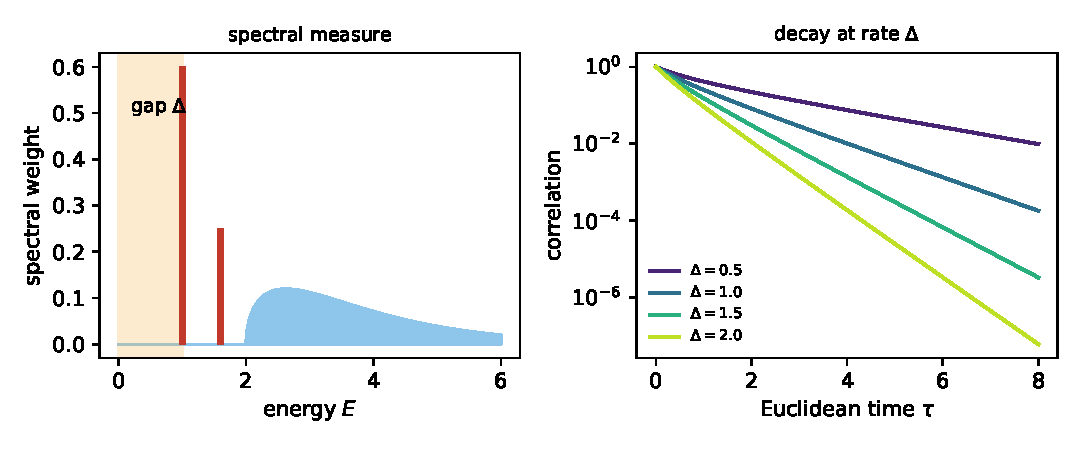
\includegraphics[width=0.95\textwidth]{figures/spectrum_gap.pdf}
\caption[A spectral measure with a gap]{Left: a spectral measure with two stable states and a continuum, and an empty interval of width $\Delta$ above the vacuum. Right: the Euclidean correlation produced by the same shape of measure shifted to four different gaps; the slope at large time is $-\Delta$.}
\label{fig:specgap}
\end{figure}

\section{The plan of the book}

The book has six parts and a closing chapter.

Chapters~\ref{ch:problem} and~\ref{ch:positivity} (Part I) set up lattice gauge theory as a probability model, explain where positivity comes from, and collect the Thorin toolkit. Chapters~\ref{ch:routeA} to~\ref{ch:hitting} (Part II) translate the gap into statements about generalized gamma convolutions along two routes, treat the gap as a parameter to estimate, and are about computation and the people whose ideas it rests on: latent variables and nested sampling, the vertical likelihood family and split sampling, Yakowitz's weighted Monte Carlo, Kac and P\'olya on models, Jerrum and Sinclair on randomised approximation, Sokal on autocorrelation, clusters and zeros, slice variables, log concavity and Besag's Markov random fields, and hitting times as a way to learn the gap. Section~\ref{ch:plgbc} applies sufficient statistics, particle learning and generative Bayesian computation to the ladder.

Chapter~\ref{ch:twod} (Part III) holds the solvable worlds: two dimensions, with a guided tour, the Riemann kernel on the three sphere, dynamic and static gaps, the renormalization group for statisticians, free fields, and large $N$.

Chapters~\ref{ch:strong} to~\ref{ch:theta} (Part IV) go to four dimensions, through strong coupling, lattice Monte Carlo for glueballs, the Migdal Kadanoff ladder and its verification, the ladder on counts and Kingman's coalescent, real zeros, and theta kernels, fermion determinants and Howe duality.

Chapters~\ref{ch:path} to~\ref{ch:sandwich} (Part V) are the path that remains and new work on the open problems: Sections~\ref{ch:isthere} and~\ref{ch:missing} assess the path and what it leaves out, and the chapters give a product formula for the SU(2) heat kernel that closes, for SU(2), the likelihood ratio problem, tests of the ladder against lattice data, an empirical sandwich between two caricatures in three and four dimensions, correlation inequalities, and the case for three dimensions first. Chapter~\ref{ch:kacyang} (Part VI), Neighbouring Problems, takes up Kac and Yang's discrete system, stochastic quantisation and filtering, Hilbert's sixth problem, and what this book owes to our Riemann and Langlands volumes. Chapter~\ref{ch:programme} lists twelve problems in order of difficulty, Section~\ref{ch:history} gives the history, and Section~\ref{ch:results} summarises what is new. The appendices contain the code, auxiliary proofs, notation, a dictionary between the languages of physics and statistics, solutions, a computational notebook and a glossary.

\section{Results at a glance}

\begin{center}
\scriptsize
\begin{tabular}{p{2.55in}p{0.85in}p{0.6in}}
\toprule
result & status & where \\ \midrule
spectral measure is a Thorin measure\index{Thorin measure}; gap is the tail index of a GGC~\cite{Th77} & theorem & Ch.~\ref{ch:routeA} \\
$2\sin^2$ transport is unconditional; Thorin density\index{Thorin density} is a L\'evy exponent\index{Levy exponent@L\'evy exponent} & theorem & Sec.~\ref{ch:routeB} \\
gap is the decay rate of the Thorin densities; constant in the uniform inequality is free & theorem & Sec.~\ref{ch:routeB} \\
correlators with two isolated levels are not GGC & theorem & Sec.~\ref{ch:routeB} \\
gap estimated as a support constraint in positive deconvolution\index{positive deconvolution} & numerical & Ch.~\ref{ch:estimation} \\
2D SU(2): $\Delta(a)\ge\Delta_{\mathrm{cont}}\operatorname{arcsinh}(x)/x$ at every spacing & theorem & Ch.~\ref{ch:twod} \\
Riemann's $\Phi$ from the return density of Brownian motion\index{Brownian motion on SU(2)} on $S^3$ & theorem & Sec.~\ref{ch:riemann} \\
Migdal Kadanoff preserves positive definiteness & theorem & Sec.~\ref{ch:mk} \\
MK decrement $(1-b^{-2})N^2\E S_{\mathrm{BPY}}/4$, within $3\%$ of one loop at $b=2$ & leading order & Sec.~\ref{ch:mk} \\
SU(3) decrement approaches $9/16$ & numerical & Sec.~\ref{ch:mk} \\
MK map monotone from a likelihood ratio\index{likelihood ratio order} property & theorem & Sec.~\ref{ch:verification} \\
decrement of the SU(2) heat kernel projected ladder positive at every coupling & theorem & Ch.~\ref{ch:progress} \\
correlation length as a first passage time\index{first passage time} & derivation & Sec.~\ref{ch:verification} \\
product formula for the SU(2) heat kernel; likelihood ratio property at every time & theorem & Ch.~\ref{ch:progress} \\
weak coupling expansion of the ladder to three orders; two loop ratio $1/(6b^2)$ & theorem & Ch.~\ref{ch:progress} \\
convolution is totally positive when $\Delta f/f$ is monotone & theorem & Ch.~\ref{ch:progress} \\
gap as Poincar\'e constant of the ground state measure & proposition & Sec.~\ref{ch:h6ym} \\
ladder against lattice data: rate within $15\%$, crossover misplaced & numerical & Ch.~\ref{ch:progress} \\
vertical likelihood, split sampling, nested sampling on exact 2D torus & numerical & Sec.~\ref{ch:vertical} \\
Yakowitz rate $n^{-2}$ in thermodynamic integration & numerical & Sec.~\ref{ch:yakowitz} \\
dynamic gap equals static gap; log Sobolev route & survey & Sec.~\ref{ch:dynamic} \\
empirical sandwich: loop laws between independent and MK caricatures & numerical & Ch.~\ref{ch:sandwich} \\
upper half of the sandwich for expectations, $W_{22}\ge W_{11}^4$, any compact group & theorem & Sec.~\ref{ch:griffiths} \\
particle learning of the decrement; GBC matching of blocked ensembles & numerical & Sec.~\ref{ch:plgbc} \\
\bottomrule
\end{tabular}
\end{center}

\begin{center}
\scriptsize
\begin{tabular}{p{2.55in}p{0.85in}p{0.6in}}
\toprule
result & status & where \\ \midrule
coalescence of the latent count is hypergeometric; Kingman duality & theorem & Ch.~\ref{ch:counts}, Sec.~\ref{ch:kingman} \\
the count is $E[1/(1-\cos\theta)]-2$; first rung drift tending to $-\frac{13}{16}$ from point masses and to $+\frac18$ from Wilson laws; the heat kernel value $-\frac12$ is numerical & theorem, numerical & Ch.~\ref{ch:counts} \\
real zeros under heat flow; smoothed criterion for convolutions & theorem & Ch.~\ref{ch:zeros} \\
closure of the real zeros class under convolution & conjecture & Ch.~\ref{ch:zeros} \\
Hartman Watson law is a generalized gamma convolution & theorem & Ch.~\ref{ch:zeros} \\
vacuum of one plaquette has real zeros; rule for registers & theorem, numerical & Sec.~\ref{ch:quantum} \\
fermion determinants, matching expansion of decimation & theorem & Ch.~\ref{ch:theta} \\
comparison of MK with $\Z^4$ at the level of spectral measures & open & Sec.~\ref{ch:isthere} \\
\bottomrule
\end{tabular}
\end{center}

Two warnings. No chapter proves the mass gap. And the Migdal Kadanoff recursion, which carries the four dimensional analysis, is exact only on hierarchical lattices; its relation to the true theory on $\Z^4$ is the central open problem of Chapter~\ref{ch:path}.

\section{Gauge theory for probabilists}\label{ch:gauge}

Lattice gauge theory is a probability model: a random field of group elements on the edges of a graph, with a Gibbs density invariant under a large symmetry group. Nothing here is new, but the probabilistic vocabulary is the one we use throughout.

\subsection{Random group elements on edges}

Let $G$ be a compact Lie group, for us SU(2) or SU(3), with normalised Haar measure\index{Haar measure} $\mathrm dU$. Let $B$ be a finite box in $\Z^d$ with periodic boundary conditions, and let $\mathcal E(B)$ be a set of links containing one orientation of each edge. A gauge field configuration assigns a group element $U_\ell\in G$ to every link $\ell$, with the convention $U_{\ell^{-1}}=U_\ell^{-1}$ for the reversed link. The configuration space is the product $G^{\mathcal E(B)}$, a compact manifold of dimension $\dim G\cdot|\mathcal E(B)|$, and the reference measure is the product Haar measure.

A plaquette $p$ is an elementary square of the lattice, with boundary links $\ell_1,\ell_2,\ell_3,\ell_4$ traversed in order. Its holonomy is the ordered product
\[
U_p=U_{\ell_1}U_{\ell_2}U_{\ell_3}U_{\ell_4}.
\]
Changing the starting corner conjugates $U_p$, and reversing the orientation inverts it. A class function of $U_p$, that is a function invariant under conjugation, is therefore well defined on unoriented plaquettes if it is also invariant under inversion.

\begin{definition}
A lattice gauge theory with plaquette weight $f$, a positive class function on $G$ with $f(U^{-1})=f(U)$, is the probability measure
\[
\mathbb P_B(\mathrm dU)=\frac{1}{Z_B}\prod_pf(U_p)\prod_\ell\mathrm dU_\ell
\]
on $G^{\mathcal E(B)}$.
\end{definition}

The Wilson weight is $f(U)=\exp(\frac\beta N\operatorname{Re}\operatorname{tr}U)$ for SU(N). The heat kernel\index{heat kernel} weight is the density of Brownian motion\index{Brownian motion on SU(2)} on $G$ at time $t$, evaluated at $U$.

Figure~\ref{fig:wilsonlaws} shows the law of the rotation angle of a single plaquette under the Wilson weight. At small $\beta$ it is close to Haar measure; as $\beta$ grows it concentrates at the identity, which is weak coupling.

\begin{figure}[t]
\centering
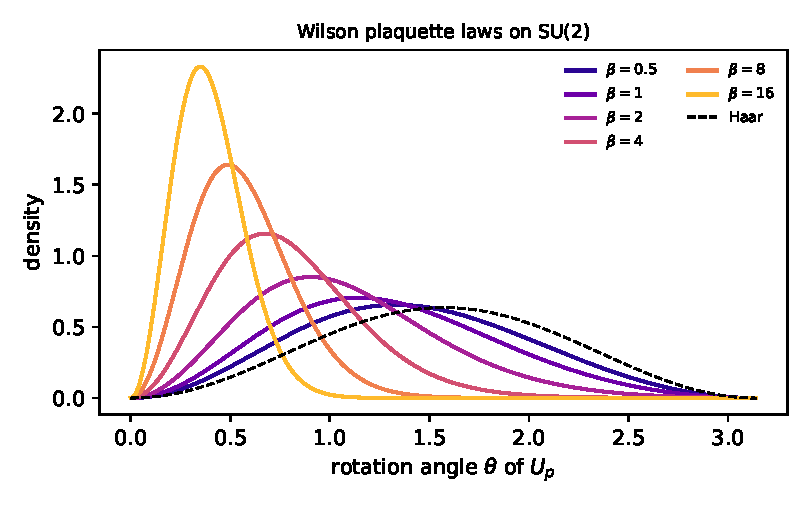
\includegraphics[width=0.85\textwidth]{figures/wilson_laws.pdf}
\caption[Wilson plaquette laws on SU(2)]{Density of the rotation angle $\theta$ of a plaquette variable under the single plaquette Wilson weight $e^{\beta\cos\theta}$ times Haar measure on SU(2), for six couplings, with the Haar density dashed.}
\label{fig:wilsonlaws}
\end{figure}

\subsection{Gauge invariance}

A gauge transformation assigns a group element $\omega_x$ to every site $x$ and acts on links by $U_{xy}\mapsto \omega_xU_{xy}\omega_y^{-1}$. Plaquette holonomies are conjugated, so class functions of them are unchanged, and Haar measure is invariant under left and right multiplication. The measure $\mathbb P_B$ is therefore invariant under the gauge group $G^{B}$, which is enormous: its dimension is comparable to that of the configuration space.

Gauge invariance has two consequences for probabilists. First, only gauge invariant observables have meaningful expectations; the expectation of any observable that is not gauge invariant is the expectation of its gauge average. On a finite box this is just the invariance of $\mathbb P_B$; Elitzur's theorem~\cite{El75} is the infinite volume statement that gauge symmetry cannot break. Second, one may fix a gauge to reduce the number of variables. In axial gauge one sets all links in one direction to the identity along a maximal tree, and, with free boundary conditions, the plaquette variables become independent in two dimensions. This is the reason two dimensional Yang Mills is solvable.

\subsection{Observables}

The basic gauge invariant observables are traces of holonomies around closed loops.
\begin{itemize}
\item The Wilson loop $W(\mathcal C)=\operatorname{tr}\prod_{\ell\in\mathcal C}U_\ell$ for a closed lattice curve $\mathcal C$. Its expectation measures the energy of a pair of static charges: for a rectangular $R\times T$ loop, $\langle W\rangle\approx e^{-V(R)T}$ for large $T$, where $V(R)$ is the static potential.
\item The plaquette observable $\operatorname{tr}U_p$, and its spatial sums at a fixed time, which project onto zero momentum glueball states. Combinations of plaquettes with definite behaviour under the lattice rotation group select the quantum numbers $J^{PC}$.
\item The Polyakov loop, the trace of the product of links along a closed curve wrapping the periodic time direction, whose expectation measures the free energy of a single static charge and serves as an order parameter for deconfinement at finite temperature.
\end{itemize}
Confinement means an area law for large Wilson loop\index{Wilson loop}s, $\langle W(\mathcal C)\rangle\le K\,e^{-\sigma\,\mathrm{Area}(\mathcal C)}$ for a constant $K$, with string tension $\sigma>0$. The mass gap\index{mass gap} concerns the correlations of local observables such as plaquettes. The two are related but distinct: in two dimensions there is confinement\index{confinement} with a string tension but no propagating particles.

\subsection{Character expansion as a Fourier expansion}

Since $f$ is a class function, it has a Fourier expansion in characters,
\[
f(U)=\sum_\lambda d_\lambda\,c_\lambda\,\chi_\lambda(U),
\]
where $\lambda$ runs over irreducible representations, $d_\lambda$ is the dimension and $\chi_\lambda$ the character. The coefficients are $c_\lambda=d_\lambda^{-1}\int f\bar\chi_\lambda\,\mathrm dU$. Two facts make this expansion the natural coordinate system.
\begin{enumerate}
\item[(i)] Convolution diagonalises: if $f*g(U)=\int f(UV^{-1})g(V)\mathrm dV$, then $c_\lambda(f*g)=c_\lambda(f)c_\lambda(g)$. Integrating out a link shared by two plaquettes in a plane is such a convolution.
\item[(ii)] Products decompose by Clebsch Gordan: $\chi_\kappa\chi_\nu=\sum_\lambda n^\lambda_{\kappa\nu}\chi_\lambda$ with nonnegative integer multiplicities $n^\lambda_{\kappa\nu}$.
\end{enumerate}
Writing $u_\lambda=c_\lambda/c_{\mathrm{triv}}$, the normalised coefficients satisfy $|u_\lambda|\le1$, and they equal the Fourier transform $\E[\chi_\lambda(U)]/d_\lambda$ of the probability law with density $f/c_{\mathrm{triv}}$. We call them Thorin levels in this book, because in Section~\ref{ch:mk} they play the role that the levels of the Thorin ladder play in our Riemann programme.

\subsection{Transfer matrices}

Choose one lattice direction as time. Group the links into time slices: the spatial links at time $\tau$ and the temporal links from $\tau$ to $\tau+1$. In temporal gauge, the temporal links are set to the identity, and the measure becomes a Markov chain in time whose state is the configuration of spatial links at time $\tau$, subject to Gauss's law. The transition kernel is the transfer matrix\index{transfer matrix} $\mathcal T$, an integral operator on $L^2$ of the spatial configuration space restricted to gauge invariant functions. Reflection positivity~\cite{OSe,Lu77}, discussed in Chapter~\ref{ch:positivity}, makes $\mathcal T$ selfadjoint and positive. The Markov chain picture has a simple consequence: correlations of time slice observables are matrix elements of powers of $\mathcal T$,
\[
\langle O_0O_n\rangle-\langle O\rangle^2=\langle O,\mathcal T^nO\rangle_0=\int\eta^n\,\mu_O(\mathrm d\eta),
\]
where $\mu_O$ now denotes the spectral measure\index{spectral measure} in the variable $\eta=e^{-aE}$. It lives on $[0,1)$ once $\mathcal T$ is normalised to have top eigenvalue $1$ and that eigenvalue, the vacuum, is removed. This is the Laplace transform representation of Chapter~\ref{ch:positivity}. The mass gap is the spectral gap of this Markov chain, in units of the lattice spacing: the distance between the top eigenvalue and the rest of the spectrum, measured on the logarithmic scale.

This makes the mass gap a close relative of a familiar probabilistic question, the rate of convergence to equilibrium of a Markov chain. The difference is that the chain here is infinite dimensional, its state space is the configuration of a whole spatial slice, and the question is whether the rate survives an infinite sequence of rescalings.

\subsection{Scales and the continuum limit}

The lattice measure contains no length; physical units enter only by holding a physical quantity, such as the lightest glueball mass, fixed as $\beta$ varies. Asymptotic freedom forces $\beta\to\infty$ as $a\to0$, so the continuum limit is taken along a curve in the space of lattice theories, the renormalized trajectory, on which the correlation length in lattice units diverges like $1/a$. A continuum gap means it diverges no faster. The renormalization group follows this curve by replacing a theory at spacing $a$ with an effective theory at spacing $ba$; Sections~\ref{ch:mk} and~\ref{ch:verification} study an approximation to it in which both asymptotic freedom and confinement are visible.

\section{Probabilists and gauge fields}\label{ch:probabilists}

The approach of this book is probabilistic, and it joins a line of work by probabilists on gauge theories that has grown substantially since the 1990s. This section surveys that line briefly, to place our contribution and to point the reader to results that bear on the mass gap\index{mass gap}. We describe each strand at the level of its main idea and avoid claims about details we have not checked.

\subsection{Two dimensional Yang Mills measures}

In two dimensions the continuum Yang Mills measure can be constructed directly as a probability measure on connections modulo gauge, or more precisely on the holonomies of loops. Driver~\cite{Dr89} and Sengupta constructed it in the plane and on surfaces in the late 1980s and early 1990s~\cite{Se97}, using that in two dimensions the holonomies along a family of nested loops behave like Brownian motion\index{Brownian motion on SU(2)} on the group. Thierry L\'evy~\cite{Le03} developed the theory systematically: the Yang Mills measure on a compact surface as a random holonomy process, its Markov property under cutting and gluing of surfaces, and its relation to Brownian motion on the structure group. The partition functions of Chapter~\ref{ch:twod} are the total masses of these measures, and the heat kernel\index{heat kernel} of Brownian motion on the group is their basic building block. The large $N$ limit, the master field, was studied by L\'evy and by Anshelevich and Sengupta~\cite{AS12} among others, and connects to free probability.

For our purposes the lesson is that in two dimensions gauge theory is, quite literally, the theory of Brownian motion on a compact group indexed by area. Chapter~\ref{ch:twod} uses exactly this, and Section~\ref{ch:mk} tries to carry it to four dimensions through the renormalization group.

The basic process is Brownian motion on SU(2), the three sphere. Figure~\ref{fig:s3bm} shows eight paths, recorded through their angle from the identity, and the law of that angle at time six of standard Brownian motion on the unit three sphere (generator one half the Laplacian, which is time twelve in the clock of the heat kernel $K_t$ used in this book), already close to the Haar density $\frac2\pi\sin^2\theta$. The two dimensional Yang Mills measure is built from the bridges of this process.

\begin{figure}[t]
\centering
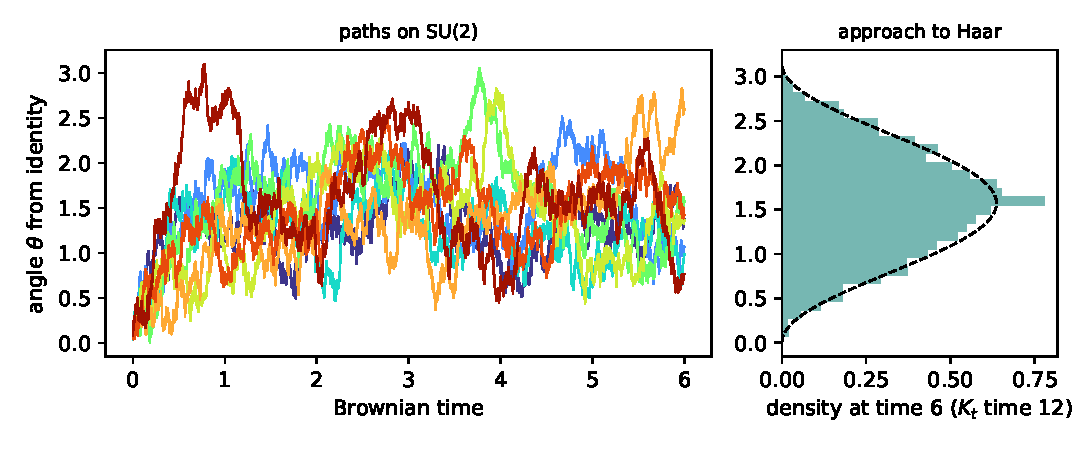
\includegraphics[width=0.95\textwidth]{figures/s3_brownian.pdf}
\caption[Brownian motion on SU(2)]{Left: eight Brownian paths on SU(2), shown through their angle from the identity. Right: the histogram of the angle at time six of standard Brownian motion (time twelve of $K_t$) from three thousand paths, against the Haar density (dashed).}
\label{fig:s3bm}
\end{figure}

\subsection{Lattice gauge theory as a probability model}

Chatterjee initiated a programme of rigorous probabilistic analysis of lattice gauge theories, with an influential survey addressed to probabilists~\cite{Ch19}. Results in this line include computations of Wilson loop\index{Wilson loop} expectations in $\Z_2$ lattice gauge theory at weak coupling, extensions by Cao~\cite{Ca20} and by Forsstr\"om, Lenells and Viklund~\cite{FLV22} to finite gauge groups, and string trajectory and surface sum representations~\cite{Ch19so,CPS25} of Wilson loop expectations at strong coupling, related to the large $N$ loop equations of Makeenko and Migdal~\cite{MM79}. Adhikari and Cao~\cite{AC} proved exponential decay of correlations, which can be read as a lattice mass gap, for lattice gauge theories with finite, possibly nonabelian, gauge groups at weak coupling.

These results are important because they treat weak coupling, the regime where the continuum limit lives, and because they are stated in probabilistic terms. The finite group case differs from the continuous group case in an essential way, however: for a finite group there is no asymptotic freedom\index{asymptotic freedom}, weak coupling is a frozen phase, and the lattice spacing does not need to shrink. The continuous group problem requires following the theory across scales, which is what the renormalization group does.

\subsection{Stochastic quantization}

A different probabilistic approach constructs the Yang Mills measure as the invariant measure of a stochastic partial differential equation, the Langevin dynamics of the Yang Mills action. Chandra, Chevyrev, Hairer and Shen constructed the Langevin dynamics for two dimensional Yang Mills, and the stochastic quantisation of three dimensional Yang Mills Higgs theory~\cite{CCHS,CCHS3}, using the theory of regularity structures~\cite{Ha14}, which handles the singular products that appear when noise is rough; Chevyrev and Shen~\cite{ChSh23} proved that the two dimensional Yang Mills measure is invariant for the renormalised dynamics. On the lattice, Shen, Zhu and Zhu~\cite{SZZ} developed a stochastic analysis approach to lattice Yang Mills at strong coupling in any dimension: Langevin dynamics, ergodicity, Poincar\'e and log Sobolev inequalities, large $N$ limits, and a mass gap for the infinite volume measure.

The stochastic quantization approach is attractive because spectral gaps of Markov dynamics are a central topic in probability, with tools such as Poincar\'e and log Sobolev inequalities and Bakry \'Emery curvature~\cite{BE}. The difficulty is that the relevant curvature is not uniformly positive in four dimensions, and controlling it is again a multiscale problem.

\subsection{Abelian theories in three dimensions}

The one complete rigorous proof of confinement\index{confinement} and a mass gap for a gauge theory at weak coupling with a nontrivial mechanism is for compact U(1) lattice gauge theory in three dimensions. Polyakov argued in 1977~\cite{Po77} that monopoles, which exist because the gauge group is compact, form a Coulomb gas whose screening gives the photon a mass and confines electric charge. G\"opfert and Mack~\cite{GM82} turned this into a theorem in 1982, proving a mass gap and an area law at all couplings. The proof is a tour de force of multiscale analysis of a Coulomb gas. It does not extend to nonabelian groups or to four dimensions, but it shows that a mass gap can be proved by following an explicit mechanism across scales.

\subsection{Hierarchical lattices}

The Migdal Kadanoff\index{Migdal Kadanoff recursion} recursion~\cite{Mi75,Ka76} used in Sections~\ref{ch:mk} and~\ref{ch:verification} is exact on hierarchical lattices, and there it has been analysed rigorously. In 1985 Ito\index{Ito, K. R.}~\cite{Ito85} proved permanent quark confinement, an area law at all couplings, for four dimensional hierarchical lattice gauge theories of Migdal Kadanoff type. Tomboulis\index{Tomboulis, E. T.}~\cite{To07} later tried to carry such bounds to $\Z^4$ by bracketing the true partition functions between Migdal Kadanoff type decimation\index{decimation}s; Ito and Seiler~\cite{IS} identified gaps in that argument in 2007 and 2008, and Tomboulis replied. Our analysis in Sections~\ref{ch:mk} and~\ref{ch:verification} works inside the same approximation and should be read against Ito's theorem: what it adds is a spectral and quantitative reading, not confinement on the hierarchical lattice itself.

\subsection{The renormalization group}

Ba\l aban\index{Balaban, T.@Ba\l aban, T.}'s series of papers in the 1980s built a rigorous renormalization group for lattice gauge theories in three and four dimensions, based on block spin transformations that average link variables over blocks and on a careful separation of small field and large field regions. It establishes ultraviolet stability: bounds on the effective actions that are uniform in the lattice spacing in the weak coupling regime. Magnen, Rivasseau and S\'eneor~\cite{MRS} constructed four dimensional SU(2) Yang Mills in a finite volume with an infrared cutoff by related methods. In both cases the analysis controls the flow from short distances down to a fixed physical scale, but not the flow into the strong coupling regime that generates the gap.

\subsection{The 2026 existence proof}

The announced 2026 existence proof is described in Section~\ref{sec:existence2026}. We treat its announced existence of a continuum theory satisfying the axioms as a working hypothesis and do not rely on the details.

\subsection{Where this book sits}

Against this background, our contribution is narrower and more specific than any of the programmes above. We do not construct measures and we do not prove a mass gap. We offer a translation of the mass gap into statements about generalized gamma convolution\index{generalized gamma convolution}s and Thorin measure\index{Thorin measure}s, built on reflection positivity\index{reflection positivity}; an exact two dimensional theorem in that language; a product formula for the SU(2) heat kernel, a coalescent description of the latent counts, and results on real zeros; a probabilistic reading of the Migdal Kadanoff renormalization group in which asymptotic freedom is the mean of a Biane Pitman Yor\index{Biane Pitman Yor variable}~\cite{BPY} variable; and a precise formulation of what would have to be compared to complete the argument. The approaches surveyed in this section are natural sources of the tools that comparison will need: L\'evy's holonomy processes for two dimensional building blocks, Ba\l aban's block spins for the true flow, and the curvature methods of stochastic quantization for the likelihood ratio\index{likelihood ratio order} comparisons of Chapter~\ref{ch:path}.

\chapter{Positivity and the Thorin Toolkit}\label{ch:positivity}

Chapter~\ref{ch:problem} posed the mass gap as a question about the support of a measure. Everything in this book rests on one structural fact: Euclidean correlations of gauge invariant observables are Laplace transforms of nonnegative measures. This chapter explains where the fact comes from, first in the axiomatic setting and then on the lattice, and records the elementary consequences we use throughout (Section~\ref{sec:wherepos}). It then collects the two toolkits used in the rest of the book. Section~\ref{ch:harmonic} gives the harmonic analysis of compact groups (characters, Casimirs, Haar measure, Brownian motion and the Jacobian of the exponential map), which is where positivity takes its group theoretic form. Section~\ref{ch:toolkit} gives the probabilistic toolkit: Stieltjes functions, generalized gamma convolutions and Thorin measures, the hyperbolic laws of Biane, Pitman and Yor, and the orders and inverse problems that the later chapters use. Most of this material is classical, and the reader who knows it may skim.

\section{Where Positivity Comes From}\label{sec:wherepos}

\subsection{Reflection positivity}

Let $\Theta$ denote reflection in the time coordinate, $\Theta(\tau,x)=(-\tau,x)$. For a Euclidean field theory with expectation $\langle\cdot\rangle$, let $\mathcal A_+$ be the algebra of observables supported in the half space $\tau>0$, and let $\Theta$ act on observables in the same way, by reflecting their support and taking complex conjugates. Osterwalder and Schrader\index{Osterwalder, K.!and Schrader, R.}~\cite{OS} showed that a Euclidean theory satisfying the condition
\begin{equation}\label{eq:RP}
\langle\Theta(F)\,F\rangle\ge0\qquad\text{for all }F\in\mathcal A_+,
\end{equation}
together with Euclidean invariance and regularity, can be continued to a relativistic quantum field theory. The construction is concrete. The form $(F,G)=\langle\Theta(F)G\rangle$ is a nonnegative inner product on $\mathcal A_+$. Quotienting by null vectors and completing gives a Hilbert space $\mathcal H$. Time translation by $r\ge0$ maps $\mathcal A_+$ to itself, and its action on $\mathcal H$ is a contraction semigroup of selfadjoint operators $e^{-rH}$ with $H\ge0$. The constant observable $1$ gives the vacuum $\Omega$.

Condition~\eqref{eq:RP} is the source of all positivity in this book. Its content is a positivity statement: the form $\langle\Theta(F)G\rangle$ is a nonnegative inner product, so $\langle\Theta(F)F\rangle\ge0$ for every $F$. It is not by itself a Markov property. For reflections in a plane of sites in a nearest neighbour model there is a stronger structure that implies it: conditioned on the time zero slice, the past and the future are independent and, if the measure is symmetric under $\Theta$, identically distributed after reflection, and then $\langle\Theta(F)F\rangle=\mathbb E\,|\mathbb E[F\mid\text{slice}]|^2\ge0$. This sufficient mechanism is not available for planes that bisect links, where the plaquettes crossing the plane couple past and future; reflection positivity still holds there, as the next subsection shows, but its proof is a different argument.

\subsection{Reflection positivity on the lattice}\label{sec:rplattice}

Osterwalder and Seiler\index{Osterwalder, K.!and Seiler, E.}~\cite{OSe} proved~\eqref{eq:RP} for lattice gauge theory with the Wilson action\index{Wilson action}, for reflections in planes that pass through lattice sites and in planes that bisect links. The argument is short enough to sketch. Write the action as $S=S_++S_-+S_0$, where $S_+$ involves only links in the upper half lattice, $S_-=\Theta S_+$, and $S_0$ collects the plaquettes that cross the reflection plane (for a plane bisecting links; a plane through sites has none). Each crossing plaquette has the form $\operatorname{tr}\big(U\,\Theta(U)^\dagger\big)$ for a product $U$ of upper links. The Boltzmann weight of the crossing plaquettes is a function $f$ of a group element $W=U\Theta(U)^\dagger$, and its character expansion\index{character expansion}
\[
f(W)=\sum_\lambda d_\lambda\,c_\lambda\,\chi_\lambda(W)
\]
has nonnegative coefficients $c_\lambda\ge0$ for the Wilson weight. Since $\chi_\lambda(U\Theta(U)^\dagger)=\sum_{ij}D^\lambda_{ij}(U)\overline{D^\lambda_{ij}(\Theta U)}$, each term is of the form $\Theta(G)G$ summed over matrix elements. Multiplying such terms and integrating against the product Haar measure\index{Haar measure} preserves nonnegativity. The same argument works for any plaquette weight whose character coefficients are nonnegative.

\begin{definition}
A class function $f$ on a compact group $G$ is positive definite if $\sum_{ij}\bar z_if(g_i^{-1}g_j)z_j\ge0$ for all finite families $g_i\in G$, $z_i\in\mathbb C$.
\end{definition}

\begin{proposition}[Bochner on a compact group]\label{prop:bochnergroup}
A continuous class function $f=\sum_\lambda d_\lambda c_\lambda\chi_\lambda$ on a compact group is positive definite if and only if $c_\lambda\ge0$ for every irreducible representation $\lambda$.
\end{proposition}

This is the compact group form of Bochner's theorem~\cite{Bc33}, and it is a classical consequence of the Peter Weyl theorem~\cite{PW27} (Section~\ref{sec:peterweyl}), quoted here without proof. The direction we use most is the easy one: if $c_\lambda\ge0$ then $f$ is positive definite, because each $\chi_\lambda(g_i^{-1}g_j)=\sum_k\langle D^\lambda(g_i)e_k,D^\lambda(g_j)e_k\rangle$ is a Gram matrix in $i,j$. The proposition tells us that the Osterwalder Seiler condition on a plaquette weight is a probabilistic condition: the weight, normalised, is the law of a random group element whose Fourier coefficients are nonnegative. We return to this in Section~\ref{ch:mk}, where every rung of a renormalization ladder will turn out to satisfy it.

L\"uscher~\cite{Lu77} completed the picture by constructing, for the Wilson action, a selfadjoint and strictly positive transfer matrix\index{transfer matrix} $\mathcal T$ on the space of gauge invariant functions of the spatial links. One lattice time step is multiplication by $\mathcal T=e^{-aH}$, normalised so that the vacuum eigenvalue is $1$ and $\|\mathcal T\|=1$, which defines the lattice Hamiltonian $H\ge0$.

Reflection positivity has a concrete matrix form. For times $\tau_i=i\delta$, the Hankel matrix $C(\tau_i+\tau_j)$ of a reflection positive correlation is positive semidefinite, because it is the Gram matrix of the states $e^{-\tau_iH}O\Omega$. Figure~\ref{fig:rphankel} contrasts a sum of three exponentials, whose Hankel matrix has three positive eigenvalues and the rest zero, with a damped cosine, which has the right decay but is not reflection positive and has a negative eigenvalue.

\begin{figure}[t]
\centering
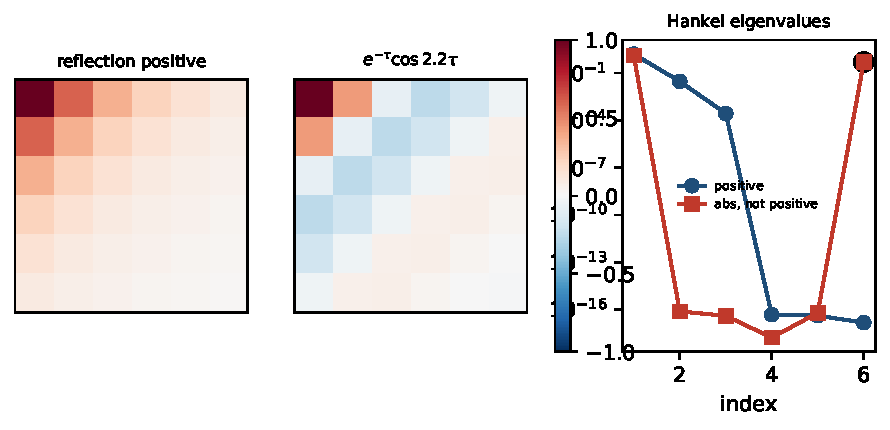
\includegraphics[width=0.95\textwidth]{figures/rp_hankel.pdf}
\caption[Reflection positivity as a Hankel condition]{Hankel matrices $C(\tau_i+\tau_j)$ on a grid of six times for a reflection positive correlation (left) and for $e^{-\tau}\cos2.2\tau$ (centre), and the absolute values of their eigenvalues (right); circled points are negative eigenvalues.}
\label{fig:rphankel}
\end{figure}

\subsection{Bernstein's theorem and the spectral measure}\label{sec:bernstein}

Fix a gauge invariant observable $O$ at zero spatial momentum and remove its vacuum expectation (we assume a unique vacuum). Then
\[
C(\tau)=\langle O,e^{-\tau H}O\rangle=\int_{(0,\infty)}e^{-\tau E}\mu(\mathrm dE),
\]
where $\mu(A)=\|P_A\,O\Omega\|^2$ for the spectral projections $P_A$ of $H$. In particular $C$ is completely monotone:
\[
(-1)^kC^{(k)}(\tau)=\int E^ke^{-\tau E}\mu(\mathrm dE)\ge0 .
\]
Conversely, Bernstein\index{Bernstein theorem}'s theorem~\cite{Be29} (see Widder's treatise on the Laplace transform~\cite{Wi41}) says that every completely monotone function on $(0,\infty)$ is the Laplace transform of a unique nonnegative measure. Complete monotonicity of the Euclidean correlation is therefore exactly equivalent to the existence of a nonnegative spectral measure\index{spectral measure}.

\begin{definition}
The gap of $O$ is $\Delta_O=\inf\operatorname{supp}\mu$. The gap of the theory is $\Delta=\inf_O\Delta_O$, the infimum over gauge invariant observables.
\end{definition}

On the lattice in finite volume, $\tau$ runs over multiples of $a$ and $C(na)=\sum_kc_k\lambda_k^n$ is a mixture of powers of the transfer matrix eigenvalues $\lambda_k=e^{-aE_k}\in(0,1)$. In the continuum $\mu$ can have atoms, the stable glueball\index{glueball}s, and a continuous part, the multiparticle states above threshold.

\subsection{The offset measure}\label{sec:offset}

For composite operators in four dimensions, $C(\tau)$ is singular at $\tau=0$. For $\operatorname{tr}F^2$ at zero momentum it grows like $\tau^{-5}$, so $\mu$ has infinite mass and quantities such as $\int_0^\infty C$ diverge. We avoid this by working at a positive Euclidean time.

\begin{definition}
For $\alpha>0$ such that $C(\alpha)<\infty$, the offset measure is $\mu_\alpha(\mathrm dE)=e^{-\alpha E}\mu(\mathrm dE)$, and the offset correlation is $C(\alpha+\tau)=\int e^{-\tau E}\mu_\alpha(\mathrm dE)$.
\end{definition}

The offset multiplies $\mu$ by a strictly positive function, so it leaves the support, and hence the gap, unchanged. It plays the same role as smearing the operator in time, or applying gradient flow at a positive flow time. Throughout, $\alpha_0$ denotes a time with $C(\alpha_0)<\infty$, and offsets are taken with $\alpha>\alpha_0$.

\subsection{First consequences}\label{sec:first}

Three elementary facts follow from positivity and are used repeatedly.

\begin{proposition}[log convexity]\label{prop:logconvex}
For $\mu\ne0$, on $\tau>\alpha_0$ (where $C$ is finite), $\tau\mapsto\log C(\tau)$ is convex. Hence the effective mass $m_{\mathrm{eff}}(\tau)=-\frac{\mathrm d}{\mathrm d\tau}\log C(\tau)$ is nonincreasing, and $m_{\mathrm{eff}}(\tau)\downarrow\Delta_O$ as $\tau\to\infty$.
\end{proposition}

\begin{proof}
For $\tau=\frac12(\tau_1+\tau_2)$, Cauchy and Schwarz give $C(\tau)^2\le C(\tau_1)C(\tau_2)$. The limit follows from Laplace's method applied to $\int e^{-\tau E}\mu(\mathrm dE)$.
\end{proof}

The proposition has a sharp methodological consequence. For the exact correlator every effective mass is an upper bound on the gap, and estimates from noisy data inherit this only up to statistical error. Numerical work can show that a claimed gap is too large, but it can never certify that a gap exists. A proof of a gap must come from analysis of the transfer matrix itself.

\begin{proposition}[mixture of exponentials]\label{prop:mixexp}
If $\int_0^\infty C(\alpha+s)\,\mathrm ds<\infty$, as when $\Delta_O>0$, the normalised offset correlation $p(\tau)=C(\alpha+\tau)/\int_0^\infty C(\alpha+s)\mathrm ds$ is a probability density on $(0,\infty)$ that is a mixture of exponential densities, with mixing measure proportional to $\mu_\alpha(\mathrm dE)/E$. By the theorem of Goldie and Steutel~\cite{Go67,St67} it is infinitely divisible.
\end{proposition}

The first two assertions are a one line computation: $p(\tau)=Z^{-1}\int Ee^{-\tau E}\,\mu_\alpha(\mathrm dE)/E$ with $Z=\int\mu_\alpha(\mathrm dE)/E=\int_0^\infty C(\alpha+s)\mathrm ds$, and $Ee^{-\tau E}$ is the exponential density with rate $E$. The infinite divisibility of exponential mixtures is the classical theorem of Goldie and Steutel, which we quote without proof.

\begin{proposition}[gap and decay]\label{prop:gapdecay}
$\Delta_O\ge m$ if and only if there is a constant $K$ with $C(\tau)\le Ke^{-m\tau}$ for all large $\tau$.
\end{proposition}

\begin{proof}
If the support is in $[m,\infty)$, then $C(\tau)\le e^{-m(\tau-\alpha_0)}C(\alpha_0)$. Conversely, if $\Delta_O<m$, a dyadic cover of $[\Delta_O,m)$ gives $\varepsilon>0$ with $\mu([m-2\varepsilon,m-\varepsilon])=c>0$, and then then $C(\tau)\ge c\,e^{-(m-\varepsilon)\tau}$, which eventually exceeds $Ke^{-m\tau}$.
\end{proof}

\subsection{Two examples}\label{sec:examples}

\begin{example}[the Wilson plaquette for SU(2)]
For SU(2) the Wilson weight of a plaquette with rotation angle $\theta$ is $e^{\beta\cos\theta}$. Its character coefficients, normalised by the trivial one, are
\[
u_n(\beta)=\frac{I_n(\beta)}{I_1(\beta)},\qquad n=1,2,3,\dots,
\]
where $n$ is the dimension of the representation and $I_\nu$ is the modified Bessel function. All are positive, and $u_2(\beta)\sim\beta/4$ as $\beta\to0$, while $u_n(\beta)\approx\exp(-(n^2-1)/(2\beta))$ as $\beta\to\infty$.
\end{example}

\begin{example}[the heat kernel plaquette]
The heat kernel\index{heat kernel} action has $u_n=e^{-t(n^2-1)/4}$ for a parameter $t>0$. At weak coupling it matches the Wilson action with $t=2/\beta$. As Section~\ref{sec:bmgroup} shows, it is the law of Brownian motion\index{Brownian motion on SU(2)} on SU(2) run for time $t$, and its coefficients multiply under convolution. This makes it the natural plaquette weight for renormalization.
\end{example}

The rest of the book takes positivity for granted and asks the other question: where do the measures live? The next two sections supply the tools for that question.

\section{Harmonic Analysis on Compact Groups}\label{ch:harmonic}

The two and four dimensional chapters (Chapters~\ref{ch:twod} and~\ref{ch:strong}) compute with characters, Casimir\index{Casimir}s, heat kernel\index{heat kernel}s and Haar measure\index{Haar measure} on SU(2) and SU(3). This section collects the facts we need, with an emphasis on the probabilistic objects: Brownian motion\index{Brownian motion on SU(2)} on a compact group, its law, and the Jacobian of the exponential map.

\subsection{The Peter Weyl theorem}\label{sec:peterweyl}

Let $G$ be a compact Lie group with Haar probability measure. The Peter Weyl theorem says that the matrix entries of the irreducible unitary representations form an orthogonal basis of $L^2(G)$, and that the characters $\chi_\lambda$ form an orthonormal basis of the class functions. Every square integrable class function has a convergent expansion $f=\sum_\lambda d_\lambda c_\lambda\chi_\lambda$, and Parseval reads $\int|f|^2=\sum_\lambda d_\lambda^2|c_\lambda|^2$.

The characters are positive definite functions, and Proposition~\ref{prop:bochnergroup} says that a class function is positive definite if and only if its coefficients are nonnegative.

\subsection{Maximal tori and the Weyl integration formula}\label{sec:weylint}

Every element of SU(N) is conjugate to a diagonal matrix $\operatorname{diag}(e^{i\theta_1},\dots,e^{i\theta_N})$ with $\sum\theta_j\equiv0\pmod{2\pi}$, unique up to permutation of the angles. A class function is therefore a symmetric function on the maximal torus. The Weyl integration formula expresses Haar integrals of class functions as torus integrals:
\[
\int_{\SU(N)}f(U)\,\mathrm dU=\frac{1}{N!}\int_{T}f(\theta)\,|V(\theta)|^2\,\mathrm d\theta,\qquad V(\theta)=\prod_{j<k}\big(e^{i\theta_j}-e^{i\theta_k}\big),
\]
with $\mathrm d\theta$ the normalised measure on the torus. For SU(2), with $\theta_1=-\theta_2=\theta$, this gives $|V|^2=4\sin^2\theta$ and the density $\frac2\pi\sin^2\theta$ on $[0,\pi]$ used throughout.

The factor $|V|^2$ is the probabilistic signature of the group: it is the Jacobian of the map from the torus times the flag manifold to the group, and it vanishes when eigenvalues collide. The eigenvalues of a Haar random unitary matrix repel each other, which is the starting point of random matrix theory.

\subsection{The Weyl character formula}\label{sec:weylchar}

Irreducible representations of SU(N) are labelled by highest weights, equivalently by partitions $\lambda_1\ge\lambda_2\ge\dots\ge\lambda_N=0$. Their characters are ratios of alternants:
\[
\chi_\lambda(\theta)=\frac{\det\big[e^{i(\lambda_j+N-j)\theta_k}\big]}{\det\big[e^{i(N-j)\theta_k}\big]}.
\]
For SU(2) this gives $\chi_n(\theta)=\sin n\theta/\sin\theta$ with $n=\lambda_1+1$ the dimension. For SU(3), labelling representations by Dynkin indices $(p,q)$, the dimension is $\frac12(p+1)(q+1)(p+q+2)$ and the quadratic Casimir is
\[
C_2(p,q)=\tfrac13\big(p^2+q^2+pq+3p+3q\big),
\]
so the fundamental representation has dimension $3$ and Casimir $4/3$. These formulas drive the SU(3) computation of Section~\ref{ch:mk}, where class functions are represented on a grid on the two dimensional torus and characters are evaluated from the Weyl formula.

\subsection{Casimirs and the Laplacian}\label{sec:casimir}

The Laplace Beltrami operator of a biinvariant metric on $G$ acts on each matrix entry of the representation $\lambda$ as multiplication by $-C_2(\lambda)$, up to a normalisation of the metric. In particular each character is an eigenfunction. For SU(2) in the normalisation of this book the eigenvalues are $(n^2-1)/4$, and the smallest nonzero one is $3/4$. For SU(N) the gap of the Laplacian is the Casimir of the fundamental representation, $(N^2-1)/(2N)$ in the standard normalisation.

\subsection{Brownian motion on a compact group}\label{sec:bmgroup}

Brownian motion on $G$ is the diffusion generated by the Laplacian, in the normalisation fixed by $K_t$ below. It is a L\'evy process on the group: its increments over disjoint time intervals are independent, and their laws are invariant under conjugation. Its law at time $t$, started from the identity, has density with respect to Haar measure
\[
K_t(U)=\sum_\lambda d_\lambda\,e^{-tC_2(\lambda)}\chi_\lambda(U),
\]
a class function with nonnegative coefficients $e^{-tC_2(\lambda)}$. The family $\{K_t\}$ is a convolution semigroup: $K_t*K_s=K_{t+s}$. Its Fourier coefficients $u_\lambda(t)=e^{-tC_2(\lambda)}$ are exponentials, and the Casimir $C_2(\lambda)$ is the rate at which the $\lambda$ coefficient decays.

Three facts about $K_t$ recur.
\begin{enumerate}
\item[(i)] As $t\to\infty$, $K_t\to1$, the Haar density, at the exponential rate set by the smallest nonzero Casimir.
\item[(ii)] As $t\to0$, $K_t$ concentrates at the identity. Near the identity the group looks like its Lie algebra, and $K_t$ is approximately a Gaussian density on $\mathfrak g$ with covariance proportional to $t$, multiplied by the Jacobian correction of the next section.
\item[(iii)] For SU(2), Poisson resummation gives the exact image formula of Section~\ref{sec:su2bm}, which expresses $K_t$ as a sum over geodesics from the identity to $U$.
\end{enumerate}

\subsection{The Jacobian of the exponential map}\label{sec:jacobian}

The exponential map $\exp:\mathfrak g\to G$ is a diffeomorphism from a neighbourhood of zero onto a neighbourhood of the identity. On class functions, written in terms of a Cartan element $X$, the Haar measure pulled back to $\mathfrak g$ has density
\[
j(X)=\prod_{\alpha>0}\Big(\frac{\sin(\alpha(X)/2)}{\alpha(X)/2}\Big)^2
\]
with respect to Lebesgue measure, where $\alpha$ runs over the positive roots. For SU(2) the single positive root gives $j=(\sin\theta/\theta)^2$. The heat kernel near the identity has the classical expansion
\[
K_t(\exp X)\approx(4\pi t)^{-\dim G/2}\,j(X)^{-1/2}\,e^{-|X|^2/(4t)}\,e^{t\,\rho^2},
\]
where $\rho$ is half the sum of the positive roots and the constant depends on normalisation. The factor $j^{-1/2}=\prod_{\alpha>0}\frac{\alpha(X)/2}{\sin(\alpha(X)/2)}$ is exactly the curvature factor of Section~\ref{ch:mk}. For SU(2) it is $\theta/\sin\theta$, and for SU(N) it is the product over the $N(N-1)/2$ pairs $p<q$ of $\frac{(\theta_p-\theta_q)/2}{\sin((\theta_p-\theta_q)/2)}$.

\subsection{Curvature factors as Laplace transforms}\label{sec:curvature}

At imaginary argument each root factor becomes $x/\sinh x$, and
\[
\frac{x}{\sinh x}=\prod_{n\ge1}\Big(1+\frac{x^2}{\pi^2n^2}\Big)^{-1}=\E\exp\Big(-\frac{x^2}{2}S_{\mathrm{BPY}}\Big),
\]
where $S_{\mathrm{BPY}}$ is the Biane Pitman Yor\index{Biane Pitman Yor variable} variable of Section~\ref{sec:bpy}, a generalized gamma convolution\index{generalized gamma convolution} with Thorin atoms at $\pi^2n^2/2$. The curvature factor of SU(N) at imaginary angle is therefore the Laplace transform of a weighted sum of $N(N-1)/2$ independent copies of $S_{\mathrm{BPY}}$. Its logarithm to second order is minus the mean, $\E S_{\mathrm{BPY}}=1/3$, times a quadratic form in the angles. That single number, multiplied by the number of positive roots and the root normalisation, will turn out, with the scale factors of the recursion, to give the coefficient of asymptotic freedom\index{asymptotic freedom} in the Migdal Kadanoff\index{Migdal Kadanoff recursion} approximation.

\subsection{Positive definiteness under products}\label{sec:pdprod}

Finally, the fact that makes the Migdal Kadanoff ladder positivity preserving. If $f$ and $g$ are class functions with nonnegative character coefficients, then so is $fg$, because
\[
\chi_\mu\chi_\nu=\sum_\lambda N^\lambda_{\mu\nu}\chi_\lambda,\qquad N^\lambda_{\mu\nu}\in\{0,1,2,\dots\}.
\]
For SU(2) the multiplicities are all zero or one, and the rule is the Clebsch Gordan\index{Clebsch Gordan rule} series $\chi_m\chi_n=\chi_{|m-n|+1}+\chi_{|m-n|+3}+\dots+\chi_{m+n-1}$. For SU(3) multiplicities greater than one occur, but they are still nonnegative integers. Positive definite functions on a compact group therefore form a cone closed under both pointwise multiplication and convolution, the two operations of renormalization.

\section{The Probabilistic Toolkit}\label{ch:toolkit}

The probabilistic objects used in the rest of the book come next. Their arrangement reflects our Riemann programme~\cite{PS26a}, where they were assembled for a different purpose.

\subsection{Laplace transforms and Stieltjes functions}\label{sec:stieltjes}

For a nonnegative measure $\nu$ on $[0,\infty)$ write $\hat\nu(s)=\int e^{-sx}\nu(\mathrm dx)$. A function $g$ on $(0,\infty)$ is a Stieltjes function\index{Stieltjes function} if
\[
g(s)=a+\int_{[0,\infty)}\frac{\sigma(\mathrm dt)}{s+t}
\]
for some $a\ge0$ and a nonnegative measure $\sigma$ with $\int(1+t)^{-1}\sigma(\mathrm dt)<\infty$. A Stieltjes function extends analytically to $\mathbb C\setminus(-\infty,0]$, and the measure is recovered from the jump across the cut:
\[
\sigma(\mathrm dt)=\lim_{\varepsilon\downarrow0}\frac{1}{\pi}\operatorname{Im}g(-t-i\varepsilon)\,\mathrm dt
\]
in the weak sense. This Stieltjes inversion formula is the main analytic tool in Chapter~\ref{ch:routeA}. The Laplace transform of a completely monotone function that is integrable near $0$, such as an offset correlation, is a Stieltjes function: if $C(\tau)=\int e^{-\tau E}\mu(\mathrm dE)$ then $\int_0^\infty e^{-s\tau}C(\tau)\mathrm d\tau=\int\mu(\mathrm dE)/(s+E)$.

\subsection{Generalized gamma convolutions}\label{sec:ggc}

The gamma law with shape $a$ and rate $t$ has Laplace transform $(1+s/t)^{-a}$. A finite convolution of gamma laws with shapes $a_j$ and rates $t_j$ has Laplace transform $\exp(-\sum_ja_j\log(1+s/t_j))$. Thorin, studying the infinite divisibility of the Pareto and log normal laws in 1977~\cite{Th77,Th77b}, introduced the closure of this class under weak limits.

\begin{definition}
A probability law on $[0,\infty)$ is a generalized gamma convolution\index{generalized gamma convolution} (GGC) if its Laplace transform has the form
\[
\varphi(s)=\exp\Big(-a s-\int_{(0,\infty)}\log\big(1+\tfrac st\big)U(\mathrm dt)\Big),
\]
with $a\ge0$ and a nonnegative measure $U$, the Thorin measure\index{Thorin measure}, satisfying $\int_{(0,1]}|\log t|\,U(\mathrm dt)<\infty$ and $\int_{(1,\infty)}t^{-1}U(\mathrm dt)<\infty$.
\end{definition}

Differentiating,
\[
-\frac{\mathrm d}{\mathrm ds}\log\varphi(s)=a+\int\frac{U(\mathrm dt)}{s+t},
\]
so a law is a GGC exactly when the logarithmic derivative of its Laplace transform is a Stieltjes function. This characterisation is what Chapter~\ref{ch:routeA} uses. Bondesson\index{Bondesson, L.}'s monograph~\cite{Bo92} develops the theory; we record the facts we need, with their proofs left to that source.

\begin{proposition}[properties of GGC, quoted from~\cite{Bo92}]\label{prop:ggcprops}
\begin{enumerate}
\item[(i)] The class is closed under convolution and under weak limits. Under weak convergence the Thorin measures converge vaguely.
\item[(ii)] Every GGC is infinitely divisible and self decomposable. Its L\'evy measure has density $k(x)/x$ with $k(x)=\int e^{-xt}U(\mathrm dt)$ completely monotone.
\item[(iii)] (Bondesson) A GGC with $a=0$ is the law of $\sum_jY_j/T_j$, where $(T_j,Y_j)$ are the points of a Poisson process on $(0,\infty)^2$ with intensity $U(\mathrm dt)\,y^{-1}e^{-y}\mathrm dy$: a shot noise of the jumps of a gamma process, rescaled by rates drawn from the Thorin measure. When $U$ has atoms of integer mass the gamma jumps can be replaced by exponential variables, as for $S_{\mathrm{BPY}}$ below.
\item[(iv)] A law with density $f$ is hyperbolically completely monotone (HCM) if $f(uv)f(u/v)$ is completely monotone in $v+1/v$ for each $u>0$. Every HCM law is a GGC.
\end{enumerate}
\end{proposition}

Part (iii) gives the probabilistic meaning of the Thorin measure: it is the intensity of the rates in a shot noise. The left edge of its support is the slowest available rate, and it sets the exponential tail of the law. Chapter~\ref{ch:routeA} uses exactly this.

\subsection{L\'evy measures and compound Poisson processes}\label{sec:levy}

A L\'evy process $X$ on $\R$ with symmetric L\'evy measure and no Gaussian part has characteristic function $\E e^{itX_1}=e^{-\psi(t)}$ with
\[
\psi(t)=\int_{\R}\big(1-\cos tx\big)\,\nu(\mathrm dx).
\]
When $\nu$ is finite, $X$ is a compound Poisson process: jumps arrive at rate $\nu(\R)$ and have law $\nu/\nu(\R)$. If $\nu$ lives on $(0,\infty)$ we symmetrise it, so that $\psi(t)=\int_{(0,\infty)}(1-\cos tx)\nu(\mathrm dx)$. Section~\ref{ch:routeB} will show that the Thorin densities produced by the $2\sin^2$ lemma are exactly such L\'evy exponent\index{Levy exponent@L\'evy exponent}s, divided by $\pi t$.

\subsection{The hyperbolic laws of Biane, Pitman and Yor}\label{sec:bpy}

Biane, Pitman and Yor~\cite{BPY} studied a family of laws attached to Brownian motion\index{Brownian motion on SU(2)} and Bessel processes whose Laplace transforms are hyperbolic functions:
\[
\E e^{-\lambda C}=\frac{1}{\cosh\sqrt{2\lambda}},\qquad
\E e^{-\lambda S_{\mathrm{BPY}}}=\frac{\sqrt{2\lambda}}{\sinh\sqrt{2\lambda}},\qquad
\E e^{-\lambda T}=\frac{\tanh\sqrt{2\lambda}}{\sqrt{2\lambda}} .
\]
The variable $C$ is the first exit time of Brownian motion from $(-1,1)$. The variable $S_{\mathrm{BPY}}$ is the first hitting time of $1$ by a three dimensional Bessel process started at $0$. These laws are tied to the Jacobi theta function, and through it to the Riemann zeta function; Biane, Pitman and Yor show that the Riemann $\xi$ function appears as a Mellin transform of a closely related law. The infinite product expansions of $\cosh$ and $\sinh$ give, for example,
\[
\frac{\sqrt{2\lambda}}{\sinh\sqrt{2\lambda}}=\prod_{n\ge1}\Big(1+\frac{2\lambda}{\pi^2n^2}\Big)^{-1},
\]
so $S_{\mathrm{BPY}}$ is a GGC with Thorin measure $\sum_n\delta_{\pi^2n^2/2}$: an infinite sum of independent exponential variables with rates $\pi^2n^2/2$. Its mean is
\[
\E S_{\mathrm{BPY}}=\sum_{n\ge1}\frac{2}{\pi^2n^2}=\frac13 .
\]
Similarly $\E C=1$ and $\E T=2/3$.

\begin{figure}[t]
\centering
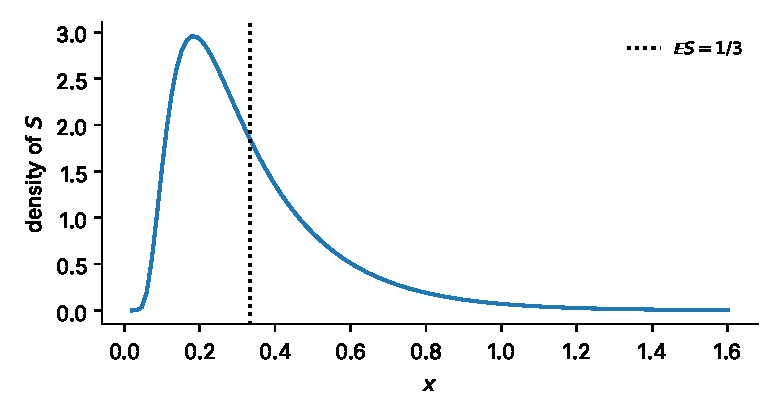
\includegraphics[width=0.92\textwidth]{figures/bpy_density.pdf}
\caption[The density of the Biane Pitman Yor variable $S_{\mathrm{BPY}}$]{The density of the Biane Pitman Yor variable $S_{\mathrm{BPY}}$, computed by numerical inversion of $\sqrt{2\lambda}/\sinh\sqrt{2\lambda}$. Its mean $1/3$ enters the coefficient of asymptotic freedom in the Migdal Kadanoff approximation of Section~\ref{ch:mk}.}
\label{fig:bpy}
\end{figure}

The P\'olya Gamma\index{Polya Gamma@P\'olya Gamma} laws of Polson, Scott and Windle~\cite{PSW13} belong to the same family. The variable $\mathrm{PG}(b,0)$ has Laplace transform $\cosh^{-b}\sqrt{\lambda/2}$, so $\mathrm{PG}(b,0)$ has the law of $C_b/4$, where $C_b$ is the sum of $b$ independent copies of $C$. The exponential tilting $\mathrm{PG}(b,c)$ is what makes Gibbs sampling for logistic models conjugate. The variable $S_{\mathrm{BPY}}$ appears in this book for a different reason, explained in Section~\ref{sec:curvature}: the inverse square root $\theta/\sin\theta$ of the Jacobian of the exponential map of SU(2), continued to imaginary angle, is its Laplace transform.

\subsection{Products and convolutions}\label{sec:prodconv}

Two operations on probability laws recur in renormalization. Given densities $f$ and $g$ with respect to a common reference measure, the normalised product $fg/\int fg$ is the posterior obtained by combining two independent pieces of evidence, and the $k$th normalised power $f^k/\int f^k$ is the posterior from $k$ independent copies of the likelihood $f$. The convolution $f*g$ is the law of a sum of independent variables, or of a product of independent group elements.

For Gaussian laws on $\R^m$ the two operations are dual in the simplest possible way:
\[
\text{product: precisions add},\qquad\text{convolution: variances add}.
\]
Polson and Scott~\cite{PSdual} develop this duality, between mixtures (convolutions) and envelopes (products), as a general principle of hierarchical modelling. In Section~\ref{ch:mk} it becomes the bookkeeping of the Migdal Kadanoff\index{Migdal Kadanoff recursion} recursion, and the failure of exact duality on a curved group is what drives asymptotic freedom\index{asymptotic freedom} in that approximation.

\subsection{Likelihood ratio orders}\label{sec:lro}

\begin{definition}
A family of densities $\{f_t\}$ on an interval has monotone likelihood ratio\index{likelihood ratio order} in $t$ if $f_{t'}(x)/f_t(x)$ is increasing in $x$ whenever $t'>t$. Equivalently, for smooth positive densities, $\partial_x\log f_t(x)$ is increasing in $t$.
\end{definition}

\begin{proposition}\label{prop:lro}
\begin{enumerate}
\item[(i)] If $\{f_t\}$ has monotone likelihood ratio, then $f_{t'}$ is stochastically larger than $f_t$ for $t'>t$, so $\int h\,f_t$ is increasing in $t$ for every increasing $h$.
\item[(ii)] Monotone likelihood ratio is preserved by normalised products with a fixed positive function, and by taking powers.
\item[(iii)] (Karlin~\cite{Ka68}) Monotone likelihood ratio is preserved by convolution with a log concave density.
\end{enumerate}
\end{proposition}

Parts (i) and (iii) are classical, and we quote them from Karlin~\cite{Ka68} without proof; part (ii) is immediate, since multiplying by a fixed positive function leaves the ratio $f_{t'}/f_t$ unchanged and powers preserve monotonicity of a positive ratio. Part (iii) is a statement about total positivity of order two; log concave densities are P\'olya frequency functions of order two, and the composition of totally positive kernels is totally positive. Section~\ref{ch:verification} uses (i) and (ii) to prove that a renormalization map is monotone. Chapter~\ref{ch:path} asks whether (iii) can survive on a curved group, where the relevant kernels are no longer log concave.

\subsection{Positive linear inverse problems}\label{sec:pliv}

Finally, recovering a nonnegative measure $\mu$ from noisy observations of a linear functional $K\mu$ is a positive linear inverse problem. Vardi and Lee\index{Vardi, Y.!and Lee, D.}~\cite{VL} gave the EM algorithm
\[
\nu^{(r+1)}=\nu^{(r)}\cdot\frac{K^\top\big(y/K\nu^{(r)}\big)}{K^\top 1},
\]
which preserves positivity and decreases a Kullback Leibler divergence (that is, increases the likelihood). Polson and Robert~\cite{PR}, in their discussion of Vardi and Lee, interpreted the inversion as a von Neumann style Monte Carlo procedure. Padilla, Polson and Scott~\cite{PPS} give Bayesian nonparametric deconvolution with theoretical guarantees, and Polson, Scott and Willard~\cite{PSW15} survey the proximal algorithms that accelerate such schemes. Chapter~\ref{ch:estimation} applies these ideas to the inverse Laplace problem of extracting a spectrum from a correlator, where the support edge, and so the gap, is far better determined than the measure itself.

\section*{Exercises}
\begin{enumerate}
\item (Section~\ref{sec:examples}) Show directly that the Wilson weight $e^{\beta\cos\theta}$ on SU(2) has positive character coefficients $u_n=I_n(\beta)/I_1(\beta)$, using the generating function $e^{\beta\cos\theta}=\sum_{m\in\Z}I_m(\beta)e^{im\theta}$ and $\chi_n(\theta)\sin\theta=\sin n\theta$.
\item (Section~\ref{sec:first}) Prove that a mixture of exponential densities is log convex, and deduce the monotonicity of the effective mass in Proposition~\ref{prop:logconvex} without using the spectral theorem.
\item (Section~\ref{sec:first}) Let $C(\tau)=\sum_{k=1}^Kc_ke^{-E_k\tau}$ with $c_k>0$ and $0<E_1<\dots<E_K$. Compute $m_{\mathrm{eff}}(\tau)$ and show that $m_{\mathrm{eff}}(\tau)-E_1$ decays like $e^{-(E_2-E_1)\tau}$.
\item (Section~\ref{sec:offset}) Show that the offset measure $\mu_\alpha$ has the same support as $\mu$, and that $\int E^{\,j}\mu_\alpha(\mathrm dE)<\infty$ for all $j$ whenever $C(\alpha_0)<\infty$ for some $\alpha_0<\alpha$.
\item (Section~\ref{sec:first}) Give an example of a nonnegative measure $\mu$ with $\inf\operatorname{supp}\mu=0$ whose Laplace transform nevertheless satisfies $C(\tau)\le K\tau^{-10}$. Explain why such a correlation can never be certified gapless from data on a finite window.
\item (Section~\ref{sec:ggc}) Show that a sum of independent gamma variables with shapes $a_j$ and rates $t_j$ is a GGC with Thorin measure $\sum_ja_j\delta_{t_j}$.
\item (Section~\ref{sec:bpy}) Compute $\E C$, $\E S_{\mathrm{BPY}}$ and $\E T$ for the three hyperbolic laws of Biane, Pitman and Yor from their Laplace transforms, and check $\E S_{\mathrm{BPY}}=\sum_n2/(\pi^2n^2)$.
\item (Section~\ref{sec:bpy}) Show that $\mathrm{PG}(1,0)$ has the law of $C/4$, and compute its variance.
\item (Section~\ref{sec:lro}) Prove that if $f_t$ has monotone likelihood ratio in $t$, so does the normalised power $f_t^k/\int f_t^k$ for every $k>0$.
\item (Section~\ref{sec:prodconv}) Show that the normalised product of two Gaussian densities on $\R^m$ with precisions $P_1,P_2$ has precision $P_1+P_2$, and that the convolution has covariance $P_1^{-1}+P_2^{-1}$.
\end{enumerate}

\part{Routes and Estimation}
\chapter{Two Routes to the Gap}\label{ch:routeA}

Chapter~\ref{ch:positivity} showed that reflection positivity gives every gauge invariant observable a nonnegative spectral measure, and equipped us with the Thorin toolkit. This chapter turns that positivity into the mass gap in two ways, and then tests both on models where the gap can be computed. Route A translates the mass gap\index{mass gap} into the language of generalized gamma convolution\index{generalized gamma convolution}s\cite{Th77,Bo92}: the spectral measure\index{spectral measure} of a gauge invariant observable, after the Euclidean offset, is itself a Thorin measure\index{Thorin measure}, and the gap becomes the exponential tail index of the associated GGC. Route B (Section~\ref{ch:routeB}) places the spectrum on the L\'evy side and uses the $2\sin^2$ lemma to transport it to a Thorin density, so that the gap becomes an exact decay rate. Section~\ref{ch:examples} then tests the two dictionaries on the Ising chain, a massless field and the two dimensional Ising model.

\section{Route A: The Spectrum as a Thorin Measure}\label{sec:routeAmain}

Route A is the more direct of the two translations.

\subsection{The Yang Mills GGC}

Fix a gauge invariant observable $O$ with spectral measure $\mu$, gap $\Delta=\inf\operatorname{supp}\mu>0$, and an offset $\alpha>\alpha_0$. The Laplace transform of the offset correlation is the Stieltjes function\index{Stieltjes function}
\[
\widehat C_\alpha(s)=\int_0^\infty e^{-sr}\,C(\alpha+r)\,\mathrm dr=\int\frac{\mu_\alpha(\mathrm dE)}{s+E},\qquad \mu_\alpha=e^{-\alpha E}\mu .
\]
Physically, $\widehat C_\alpha$ is the zero momentum propagator of $O$ in a Laplace energy variable. Comparing with the logarithmic derivative of a GGC suggests integrating it.

\begin{proposition}[the Yang Mills GGC]\label{prop:ymggc}
The function
\[
\varphi_\alpha(s)=\exp\Big(-\int_0^s\widehat C_\alpha(r)\,\mathrm dr\Big)=\exp\Big(-\int\log\big(1+\tfrac sE\big)\mu_\alpha(\mathrm dE)\Big)
\]
is the Laplace transform of a GGC $X_\alpha$ with Thorin measure $\mu_\alpha$.
\end{proposition}

\begin{proof}
The two expressions agree because $\frac{\mathrm d}{\mathrm ds}\log(1+s/E)=1/(s+E)$ and both vanish at $s=0$. The Thorin conditions hold: $\mu_\alpha$ vanishes on $(0,\Delta)$, so the condition at the origin is trivial, and $\int_{(1,\infty)}E^{-1}\mu_\alpha(\mathrm dE)\le\int e^{-\alpha E}\mu(\mathrm dE)=C(\alpha)<\infty$.
\end{proof}

Simple spectra show the construction. If $\mu_\alpha=w\,\delta_m$ is a single stable particle of mass $m$ with weight $w$, then $X_\alpha$ is gamma distributed with shape $w$ and rate $m$. If the spectrum is a finite set of stable states, $X_\alpha$ is a sum of independent gamma variables, one per state, with shapes equal to the offset residues and rates equal to the masses. A continuous spectrum above a threshold contributes a continuous Thorin density\index{Thorin density}, and by Bondesson\index{Bondesson, L.}'s representation\cite{Bo92} an infinite shot noise of gamma process jumps, rescaled by rates equal to the multiparticle energies. Precisely, $X_\alpha=\sum_jY_j/E_j$, where $(E_j,Y_j)$ are the points of a Poisson process on $(0,\infty)^2$ with intensity $\mu_\alpha(\mathrm dE)\,y^{-1}e^{-y}\mathrm dy$.

\subsection{The gap is the tail index}

\begin{theorem}[gap as exponential moment threshold]\label{thm:abscissaB}
$\E e^{\lambda X_\alpha}<\infty$ for $\lambda<\Delta$, and $\E e^{\lambda X_\alpha}=\infty$ for $\lambda>\Delta$. Equivalently, the abscissa of convergence of $\varphi_\alpha$ is $-\Delta$, and the left edge of the Thorin support is the gap.
\end{theorem}

\begin{proof}
For $\lambda<\Delta$, the function $\log(1-\lambda/E)$ is bounded on $[\Delta,\infty)$ and of order $\lambda/E$ at infinity, so $\int\log(1-\lambda/E)\mu_\alpha(\mathrm dE)$ converges. By Campbell's theorem for the Poisson representation of Section~\ref{sec:routeAmain}, $\E e^{\lambda X_\alpha}=\exp\big(\int\!\!\int(e^{\lambda y/E}-1)y^{-1}e^{-y}\mathrm dy\,\mu_\alpha(\mathrm dE)\big)=\exp\big(-\int\log(1-\lambda/E)\,\mu_\alpha(\mathrm dE)\big)=\varphi_\alpha(-\lambda)<\infty$.

Suppose now that $\E e^{\lambda X_\alpha}<\infty$ for some $\lambda>\Delta$. A Laplace transform of a positive measure is analytic in the open half plane to the right of its abscissa, so $\varphi_\alpha$ is analytic on $\operatorname{Re}s>-\lambda$, a region containing a complex disc $N$ centred at $-\Delta$. Since $\varphi_\alpha(-\Delta)=\E e^{\Delta X_\alpha}>0$, after shrinking $N$ the function $\log\varphi_\alpha$ is analytic on $N$. On the part of $N$ off the negative real axis, $(\log\varphi_\alpha)'=-\widehat C_\alpha$, where $\widehat C_\alpha(s)=\int(s+E)^{-1}\mu_\alpha(\mathrm dE)$ is the Stieltjes transform. Hence $\widehat C_\alpha$ continues analytically across the segment $N\cap(-\infty,-\Delta]$ of its cut. By Stieltjes inversion, $\mu_\alpha$ then gives no mass to $\{E>\Delta:-E\in N\}$. An atom at $\Delta$ is also excluded, since it would make $-\Delta$ a pole of $\widehat C_\alpha$. This contradicts $\Delta\in\operatorname{supp}\mu_\alpha$.
\end{proof}

\begin{corollary}
$\liminf_{x\to\infty}\,-x^{-1}\log\Pr(X_\alpha>x)=\Delta$.
\end{corollary}

\begin{proof}
For a nonnegative random variable, Chebyshev's inequality gives $\Pr(X>x)\le e^{-\lambda x}\E e^{\lambda X}$, so $\liminf-x^{-1}\log\Pr(X>x)\ge\Delta$. Conversely, if the liminf exceeded $\Delta$, summation by parts would make $\E e^{\lambda X}$ finite for some $\lambda>\Delta$, contradicting Theorem~\ref{thm:abscissaB}. For a general random variable this gives only the liminf, since the tail may be irregular along a sparse sequence; that the limit exists for a GGC needs the GGC structure and is not proved here.
\end{proof}

The mass gap is therefore the exponential moment threshold of the Yang Mills GGC, and its tail index in the liminf sense of the corollary. In Bondesson's shot noise picture this is transparent: the variable is a sum of gamma process jumps rescaled by rates drawn from the spectrum, and the exponential moments are governed by the slowest rate, which is the lightest state.

\begin{figure}[t]
\centering
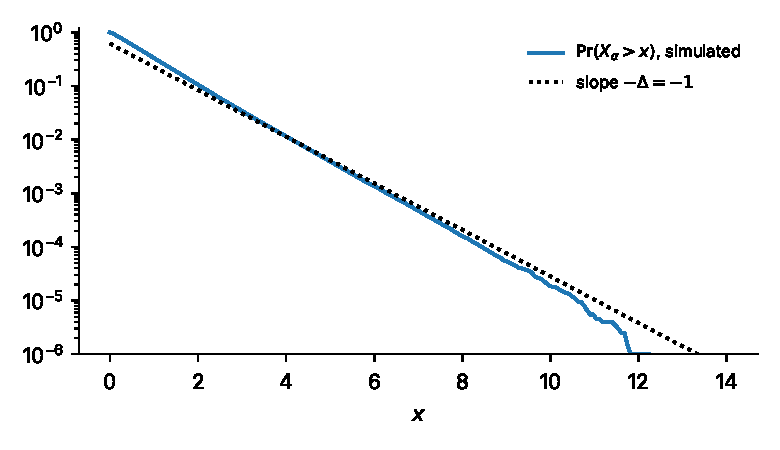
\includegraphics[width=0.92\textwidth]{figures/routeA_tail.pdf}
\caption[Route A for a toy spectrum: stable states at $1,1.5,1.9$ and a continuum from $2$, offset $\alpha=1/2$]{Route A for a toy spectrum: stable states at $1,1.5,1.9$ and a continuum from $2$, offset $\alpha=1/2$. Two million samples of the Yang Mills GGC were drawn, each a sum of independent gamma variables, one per Thorin atom, with the continuum discretised into 3000 atoms. The log tail is asymptotically linear with slope $-\Delta=-1$; the fitted slope over the visible range is $-1.06$, steeper because of the polynomial factor $x^{w-1}$ contributed by the lightest atom.}
\label{fig:routeAtail}
\end{figure}

\subsection{The Clay statement in Route A language}

The problem asks for a single $\Delta>0$ that bounds the gaps of all gauge invariant observables in the continuum theory. In Route A language this reads as follows.

\begin{quote}
For every gauge invariant observable $O$, the Yang Mills GGC $X_{O,\alpha}$ has $\E e^{\lambda X_{O,\alpha}}<\infty$ for all $\lambda<\Delta$.
\end{quote}

The continuum theory is a limit of lattice theories, and the following closure property shows what is needed.

\begin{proposition}\label{prop:closureA}
Let $\mu^{(a)}_\alpha$ be offset lattice spectral measures, in physical units, converging weakly to $\mu_\alpha$ as $a\to0$. If $\Delta_0>0$ and $\operatorname{supp}\mu^{(a)}_\alpha\subset[\Delta_0,\infty)$ for all $a$, then $\operatorname{supp}\mu_\alpha\subset[\Delta_0,\infty)$, and the GGC laws $X^{(a)}_\alpha$ converge weakly to $X_\alpha$.
\end{proposition}

\begin{proof}
The set of measures supported in the closed set $[\Delta_0,\infty)$ is closed under weak convergence. For each $s\ge0$ the function $E\mapsto\log(1+s/E)\le s/\Delta_0$ is bounded and continuous on $[\Delta_0,\infty)$, so weak convergence of the Thorin measures gives convergence of the Laplace transforms $\varphi^{(a)}_\alpha(s)$, hence weak convergence of the GGC laws.
\end{proof}

So a lattice gap that is uniform in the spacing, measured in physical units, passes to the limit. The difficulty, which no closure property can remove, is proving that uniformity.

\subsection{What Route A adds}

Route A is a change of language; its value is what the language brings. First, GGCs are closed under convolution, so independent sectors combine by convolving their GGCs and the gap of the combination is the minimum of the gaps. Second, Bondesson's shot noise representation\cite{Bo92} makes spectral quantities simulable; in the Riemann setting the candidate Thorin measure is not known to be positive and the shot noise may not exist, but here it always does. Third, the singularity of $\varphi_\alpha$ nearest the origin sits at $-\Delta$, which is the K\"all\'en Lehmann statement that the spectral density vanishes below the first threshold.

Route A gives no mechanism for keeping the support away from zero. That needs a parameter that can be driven to infinity. The Euclidean offset $\alpha$ is that parameter, and the $2\sin^2$ lemma of Route B (Section~\ref{ch:routeB}) exploits it.

\section{Route B: The 2 sin\texorpdfstring{$^2$}{2} Lemma and L\'evy Exponents}\label{ch:routeB}

Route A placed the spectrum on the Thorin side of a GGC. Route B places it on the L\'evy side, and uses the lemma at the centre of our Riemann programme\cite{PS26a} to transport it to a Thorin density\index{Thorin density}. The result is a family of Thorin densities indexed by Euclidean time, and the gap becomes their exact rate of decay.

\subsection{The lemma}

\begin{lemma}[the Polson $2\sin^2$ lemma]\label{lem:2sin2B}
For $x,w>0$ and $u=w^2/2$,
\[
e^{-wx}+wx-1=\int_0^\infty\log\Big(1+\frac uz\Big)\,k_x(z)\,\mathrm dz,
\]
where
\[
k_x(z)=\frac{x}{\pi\sqrt{2z}}\;2\sin^2\!\big(x\sqrt{z/2}\big)\ge0 .
\]
\end{lemma}

\begin{proof}
Substitute $z=2y^2$, so $\mathrm dz=4y\,\mathrm dy$ and $\sqrt{2z}=2y$. The right side becomes
\[
\frac{4x}{\pi}\int_0^\infty\sin^2(xy)\,\log\Big(1+\frac{a^2}{y^2}\Big)\mathrm dy,\qquad a=\frac w2 .
\]
Write $\sin^2(xy)=\frac12(1-\cos2xy)$ and use the two classical integrals
\[
\int_0^\infty\log\Big(1+\frac{a^2}{y^2}\Big)\mathrm dy=\pi a,
\]
\[
\int_0^\infty\log\Big(1+\frac{a^2}{y^2}\Big)\cos(2xy)\,\mathrm dy=\frac{\pi}{2x}\big(1-e^{-2ax}\big).
\]
The right side equals $\frac{4x}{\pi}\cdot\frac12\big(\pi a-\frac{\pi}{2x}(1-e^{-2ax})\big)=wx-1+e^{-wx}$.
\end{proof}

The left side is the compensated Laplace exponent of a single jump of size $x$; the right side is a Thorin integral with a nonnegative density. Integrating against a nonnegative L\'evy measure therefore produces a nonnegative Thorin measure\index{Thorin measure}. In the Riemann programme the relevant L\'evy measure, built from the primes, is signed inside the critical strip, and positivity of the transported Thorin measure is tied to the absence of zeros in a region, as developed in the Riemann volumes\cite{PS26a}; nothing here depends on that statement. In Yang Mills the L\'evy measure is the spectral measure\index{spectral measure}, and it is nonnegative by reflection positivity\index{reflection positivity}.

\subsection{The compensated increment}

Integrate the lemma against $\mu_\alpha(\mathrm dE)/E$ with $x=E$:
\[
L_\alpha(w)=\int\big(e^{-wE}+wE-1\big)\frac{\mu_\alpha(\mathrm dE)}{E}.
\]
Differentiating in $w$ gives $L_\alpha'(w)=\int(1-e^{-wE})\mu_\alpha(\mathrm dE)=C(\alpha)-C(\alpha+w)$, and $L_\alpha(0)=0$, so
\[
L_\alpha(w)=\int_0^w\big(C(\alpha)-C(\alpha+s)\big)\mathrm ds\ \ge0 .
\]
It is finite because $e^{-wE}+wE-1\le wE$. In words, $L_\alpha(w)$ is the area between the flat line at height $C(\alpha)$ and the decaying correlation over the window $[\alpha,\alpha+w]$.

\subsection{The Thorin density is a L\'evy exponent}

\begin{theorem}\label{thm:thorinB}
For $\alpha>\alpha_0$, the function $u\mapsto\exp\big(-L_\alpha(\sqrt{2u})\big)$ is the Laplace transform of a GGC whose Thorin measure has density
\[
T_\alpha(z)=\frac{\psi_\alpha(t)}{\pi t},\qquad t=\sqrt{2z},
\]
where
\[
\psi_\alpha(t)=\int(1-\cos tE)\,\mu_\alpha(\mathrm dE)=C(\alpha)-\operatorname{Re}C(\alpha+it)
\]
is the L\'evy exponent\index{Levy exponent@L\'evy exponent} of the symmetric compound Poisson process whose jump measure is $\mu_\alpha$ symmetrised (jumps $\pm E$, each with weight $\frac12\mu_\alpha(\mathrm dE)$).
\end{theorem}

\begin{proof}
All integrands are nonnegative, so Tonelli's theorem allows the exchange of the $E$ and $z$ integrals. Lemma~\ref{lem:2sin2B} gives the Thorin representation with density $\int k_E(z)\mu_\alpha(\mathrm dE)/E$, and $x\sqrt{z/2}=tE/2$ together with $2\sin^2(tE/2)=1-\cos tE$ gives the stated form. The Thorin conditions hold because $\psi_\alpha\le2C(\alpha)$, so $T_\alpha(z)=O(z^{-1/2})$ at infinity, and $\psi_\alpha(t)\sim\frac12m_2t^2$ as $t\to0$ with $m_2=\int E^2\mu_\alpha(\mathrm dE)<\infty$.
\end{proof}

The theorem has a direct quantum mechanical meaning. Let $\Psi=e^{-\alpha H/2}O\Omega$ be the state obtained by evolving the observable for Euclidean time $\alpha/2$. Then
\[
C(\alpha+it)=\langle\Psi,e^{-itH}\Psi\rangle,
\]
the return amplitude of $\Psi$ after real time $t$. So $\psi_\alpha(t)/C(\alpha)$ is the deficit $1-\operatorname{Re}\langle\Psi,e^{-itH}\Psi\rangle/\|\Psi\|^2$ of the normalised return amplitude. Nonnegativity of the Thorin density is the Cauchy and Schwarz inequality $|\langle\Psi,e^{-itH}\Psi\rangle|\le\|\Psi\|^2$. The Thorin variable $z$ is real time in disguise, through $t=\sqrt{2z}$.

The parallel with the Riemann programme is exact enough to tabulate.
\begin{center}
\small
\begin{tabular}{lll}
\toprule
 & reciprocal Xi & Yang Mills \\ \midrule
L\'evy side & primes, jumps $\log p$ & spectrum, jumps $E$ \\
Thorin side & zero ordinates, $\gamma=\sqrt{2z}$ & real time, $t=\sqrt{2z}$ \\
level parameter & abscissa $\alpha$ & Euclidean time $\alpha$ \\
positivity of $T_\alpha$ & open in the strip & Cauchy and Schwarz \\
hard question & is $T_\alpha\ge0$? & how fast does $T_\alpha$ decay? \\
\bottomrule
\end{tabular}
\end{center}

\subsection{The gap is the decay rate}

\begin{theorem}[gap as Thorin decay rate]\label{thm:rateB}
Let $\Delta=\inf\operatorname{supp}\mu$.
\begin{enumerate}
\item[(i)] For all $z>0$ and $\alpha\ge\alpha'>\alpha_0$, $T_\alpha(z)\le e^{-\Delta(\alpha-\alpha')}T_{\alpha'}(z)$.
\item[(ii)] For all but countably many $z$, $\lim_{\alpha\to\infty}-\alpha^{-1}\log T_\alpha(z)=\Delta$.
\item[(iii)] For each $z$ with $T_\alpha(z)>0$, $\alpha\mapsto\log T_\alpha(z)$ is convex, so the local rate $r_\alpha(z)=-\partial_\alpha\log T_\alpha(z)$ is nonincreasing, and for $z$ outside the exceptional countable set of (ii) it decreases to $\Delta$.
\end{enumerate}
\end{theorem}

\begin{proof}
(i) On the support, $e^{-\alpha E}=e^{-(\alpha-\alpha')E}e^{-\alpha' E}\le e^{-(\alpha-\alpha')\Delta}e^{-\alpha' E}$, and the kernel $1-\cos tE$ is nonnegative.

(ii) The bound (i) gives $\liminf-\alpha^{-1}\log T_\alpha(z)\ge\Delta$. For the reverse inequality, $q_t(E)=1-\cos tE$ vanishes only on the lattice $2\pi\Z/t$. Only countably many values of $t$ place one of the countably many atoms of $\mu$ on that lattice, and the continuous part of $\mu$ gives zero mass to every countable set. For any other $t$ and any $\varepsilon>0$, $c=\int_{[\Delta,\Delta+\varepsilon]}q_t\,\mathrm d\mu>0$, and $T_\alpha(z)\ge(\pi t)^{-1}c\,e^{-\alpha(\Delta+\varepsilon)}$.

(iii) $T_\alpha(z)$ is, as a function of $\alpha$, the Laplace transform of the nonnegative measure $(\pi t)^{-1}q_t(E)\mu(\mathrm dE)$, hence log convex by H\"older's inequality. A log convex function whose logarithm decays at rate $\Delta$ has local rate decreasing to $\Delta$.
\end{proof}

Part (iii) repeats the lesson of Proposition~\ref{prop:logconvex}: every local rate computed from data bounds the gap from above.

\begin{figure}[t]
\centering
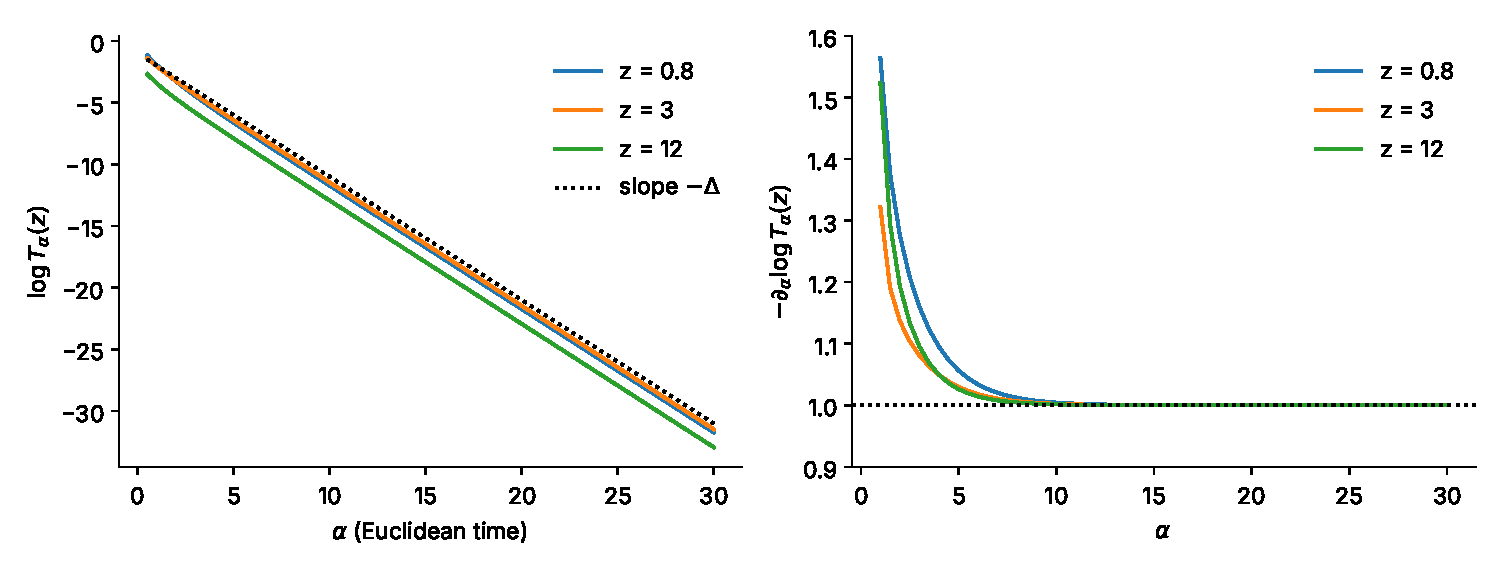
\includegraphics[width=\textwidth]{figures/thorin_gap.pdf}
\caption[Route B for the toy spectrum of Figure~\ref{fig:routeAtail}. Left: $\log T_\alpha(z)$ against]{Route B for the toy spectrum of Figure~\ref{fig:routeAtail}. Left: $\log T_\alpha(z)$ against Euclidean time for three values of $z$. Right: the local rates decrease monotonically to the gap $\Delta=1$. The real time formula of Theorem~\ref{thm:thorinB} agrees with the direct integral to ten digits; the two integrands are algebraically identical, so this checks the numerical evaluation only.}
\label{fig:thorinB}
\end{figure}

\subsection{The constant is free}

The continuum problem concerns a family of measures $\mu^{(a)}$ indexed by the lattice spacing. The natural uniform statement in Route B is an inequality between Thorin densities, and its constant carries no information.

\begin{theorem}[equivalences]\label{thm:equivB}
Let $\{\mu^{(a)}\}$ be nonnegative measures on $(0,\infty)$ with $\sup_a\int e^{-\alpha_0E}\mu^{(a)}(\mathrm dE)<\infty$, and let $m>0$. The following are equivalent.
\begin{enumerate}
\item[(a)] $\operatorname{supp}\mu^{(a)}\subset[m,\infty)$ for every $a$.
\item[(b)] There are $M'$ and $\tau_0$ with $C^{(a)}(\tau)\le M'e^{-m\tau}$ for all $\tau\ge\tau_0$ and all $a$.
\item[(c)] There is $M<\infty$ with $T^{(a)}_\alpha(z)\le Me^{-m(\alpha-\alpha')}T^{(a)}_{\alpha'}(z)$ for all $a$, all $z$ and all $\alpha\ge\alpha'>\alpha_0$.
\item[(d)] Statement (c) holds with $M=1$.
\end{enumerate}
\end{theorem}

\begin{proof}
(a) implies (d) by Theorem~\ref{thm:rateB}(i), and (d) implies (c) trivially. If (c) holds, then for fixed $a$ and $\alpha'$ the decay rate of $T^{(a)}_\alpha(z)$ is at least $m$, and Theorem~\ref{thm:rateB}(ii) gives (a). Finally (a) and (b) are equivalent by Proposition~\ref{prop:gapdecay}, whose constants are uniform under the hypothesis.
\end{proof}

We call (c) the uniform Thorin gap inequality. The theorem says that it is exactly a uniform spectral gap, that it can always be stated with $M=1$, and that it is equivalent to uniform exponential decay of correlations. Combining with weak convergence gives the continuum statement.

\begin{corollary}[continuum]\label{cor:continuumB}
If lattice measures in physical units have offset measures $e^{-\alpha_0E}\mu^{(a)}$ converging weakly, and satisfy the uniform Thorin gap inequality with one $m=\Delta_0$, then the continuum theory has a gap of at least $\Delta_0$.
\end{corollary}

\begin{proof}
For $\alpha>\alpha_0$ the kernel $e^{-(\alpha-\alpha_0)E}(1-\cos tE)$ is bounded and continuous in $E$, so $T^{(a)}_\alpha(z)\to T_\alpha(z)$ pointwise. The inequality passes to the limit, and Theorem~\ref{thm:rateB}(ii) applies.
\end{proof}

\subsection{Correlators are not themselves GGC}

Is the normalised correlation $C(\alpha+\tau)$ itself a GGC in the variable $\tau$, or even HCM? It is not, as soon as the spectrum has two isolated levels.

\begin{proposition}\label{prop:notggcB}
If $\int_0^\infty C(\alpha+s)\,\mathrm ds<\infty$ and $\mu$ has atoms at $E_1<E_2$ with $\mu((E_1,E_2))=0$, then the probability density proportional to $C(\alpha+\tau)$ is not a GGC, and hence not HCM.
\end{proposition}

\begin{proof}
Its Laplace transform is proportional to $\widehat p(s)=\int\mu_\alpha(\mathrm dE)/(E+s)$. On the interval $(-E_2,-E_1)$ the function $\widehat p$ is real analytic and strictly decreasing, since $\widehat p'(s)=-\int(E+s)^{-2}\mu_\alpha(\mathrm dE)<0$, and it runs from $+\infty$ near $-E_2$ to $-\infty$ near $-E_1$. It therefore vanishes at some $-\zeta$ with $E_1<\zeta<E_2$. If the density were a GGC with Thorin measure $U$, then $-(\log\widehat p)'=\int U(\mathrm dt)/(s+t)$ would be a Stieltjes function\index{Stieltjes function}. But near $-\zeta$ the function $-\widehat p'/\widehat p$ is meromorphic with a simple pole of residue $-1$, and Stieltjes inversion then gives $U=-\delta_\zeta$ near $\zeta$, which is negative. HCM laws are GGC, so the density is not HCM either.
\end{proof}

For the toy spectrum of Figure~\ref{fig:routeAtail}, including its continuum, at offset $\alpha=1/2$ the negative Thorin atoms sit at $1.3216$ and $1.8208$ (\texttt{code/op1\_checks.py}). In lattice SU(3) the scalar channel has two stable states below the two glueball\index{glueball} threshold\cite{MP}, so that channel is not a GGC in Euclidean time. This is why both Routes A and B build their GGCs indirectly, by integrating a Stieltjes function or by transporting a L\'evy measure, rather than asking the correlation itself to be a GGC.

\section{Models Where the Gap Can Be Computed}\label{ch:examples}

Before moving on, we test the two dictionaries on models where the spectrum is known exactly. The examples are chosen to show three behaviours: a gap that survives a renormalization flow, no gap at all, and a gap that closes at a critical point. Yang Mills is expected to behave like the first, and the contrast with the other two clarifies what the uniform Thorin gap inequality does and does not demand.

\subsection{The Ising chain and exact decimation}

The one dimensional Ising\index{Ising model} model with coupling $K$ has spins $\sigma_i=\pm1$ and weight $\exp(K\sum_i\sigma_i\sigma_{i+1})$. Its transfer matrix\index{transfer matrix} $\begin{pmatrix}e^K&e^{-K}\\ e^{-K}&e^K\end{pmatrix}$ has eigenvalues $2\cosh K$ and $2\sinh K$, and the spin correlation is
\[
\langle\sigma_0\sigma_n\rangle=(\tanh K)^n=e^{-n\,m(K)},\qquad m(K)=-\log\tanh K .
\]
The spectral measure\index{spectral measure} of the spin observable is a single atom at $m(K)$, so in Route A the GGC $X_\alpha$ is a gamma variable with rate $m(K)$, and in Route B the Thorin density\index{Thorin density} is a single damped oscillation. The gap is positive for every finite $K$, and it closes only at zero temperature, $K\to\infty$, where $m(K)\approx2e^{-2K}$ (Figure~\ref{fig:examplesgaps}).

The chain also has an exact renormalization group. Summing out every other spin gives a chain with coupling $K'$ satisfying
\[
\tanh K'=(\tanh K)^2,
\]
and more generally $\tanh K\mapsto(\tanh K)^b$ for decimation\index{decimation} by $b$. In the variable $u=\tanh K$ decimation is exactly $u\mapsto u^b$, the same form as the decimation of two dimensional Yang Mills in Chapter~\ref{ch:twod}, where character coefficients are raised to the power $b^2$. The resemblance is not an accident. Two dimensional $\Z_2$ lattice gauge theory is equivalent to a product of independent Ising chains, and the variable $u$ is the single nontrivial character coefficient of the plaquette weight. The correlation length $1/m(K)$, measured in lattice units, is divided by $b$ at each step, and the flow runs from any finite $K$ to $K=0$, the disordered fixed point. The continuum limit $K\to\infty$ requires the lattice spacing to shrink like $e^{-2K}$, and in those units the gap is constant. This is a toy version of asymptotic freedom\index{asymptotic freedom}.

\subsection{A massless field}

Next consider a theory with no gap. For a free massless field, or at a critical point, the zero momentum correlation of a suitable composite observable decays like a power, $C(\tau)\propto\tau^{-\kappa}$ for some $\kappa>0$. By Bernstein\index{Bernstein theorem}'s theorem~\cite{Be29} the spectral measure is
\[
\mu(\mathrm dE)=\frac{E^{\kappa-1}}{\Gamma(\kappa)}\,\mathrm dE,
\]
supported down to zero. In Route A the offset measure $e^{-\alpha E}E^{\kappa-1}\mathrm dE/\Gamma(\kappa)$ is a Thorin measure\index{Thorin measure} with no gap at the origin, and the Yang Mills GGC has $\E e^{\lambda X_\alpha}=\infty$ for every $\lambda>0$: its tail is heavier than any exponential. In Route B,
\[
\begin{aligned}
T_\alpha(z)&=\frac{1}{\pi t\,\Gamma(\kappa)}\int_0^\infty E^{\kappa-1}e^{-\alpha E}(1-\cos tE)\,\mathrm dE\\
&=\frac{1}{\pi t}\Big(\alpha^{-\kappa}-\operatorname{Re}(\alpha+it)^{-\kappa}\Big),
\end{aligned}
\]
which decays like a power of $\alpha$. The local rate $-\partial_\alpha\log T_\alpha(z)$ tends to zero like $(\kappa+2)/\alpha$ (Figure~\ref{fig:masslessrates}). No inequality of the form $T_\alpha\le Me^{-m(\alpha-\alpha')}T_{\alpha'}$ can hold with $m>0$. This is what the absence of a gap looks like in the Thorin language: the family of Thorin densities is still positive and still monotone, but its decay is polynomial.

\begin{figure}[t]
\centering
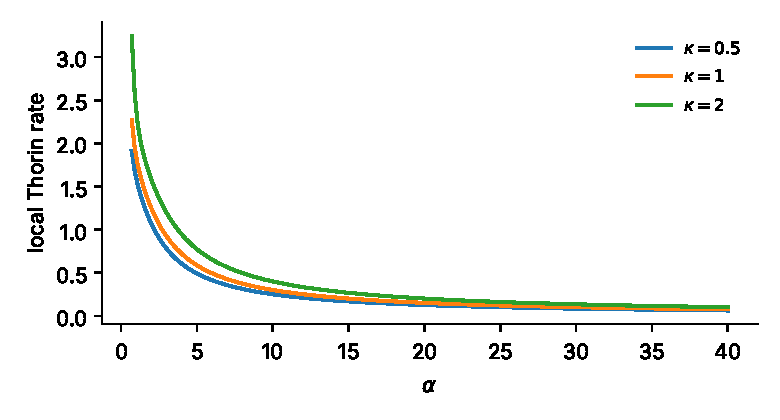
\includegraphics[width=0.92\textwidth]{figures/massless_rates.pdf}
\caption[Route B local Thorin rates for a massless spectrum $\mu(\mathrm dE)\propto E^{\kappa-1}\mathrm dE$,]{Route B local Thorin rates for a massless spectrum $\mu(\mathrm dE)\propto E^{\kappa-1}\mathrm dE$, with $t=1.3$ and $\kappa=0.5,1,2$. The rates decrease to zero like $(\kappa+2)/\alpha$; there is no gap.}
\label{fig:masslessrates}
\end{figure}

\subsection{The two dimensional Ising model}

The third example has a gap that closes at a critical point. For the two dimensional Ising model on the square lattice with coupling $K$, Onsager \cite{On44} and Kaufman \cite{Kau49} diagonalised the row to row transfer matrix. Define the dual coupling $K^*$ by $\tanh K^*=e^{-2K}$. The critical point is the self dual point $K_c=\frac12\log(1+\sqrt2)$, and the gap of the transfer matrix, in lattice units, is
\[
G(K)=2\,|K-K^*| .
\]
It is positive on both sides of $K_c$ and vanishes linearly at $K_c$, so the correlation length diverges like $|K-K_c|^{-1}$ (Figure~\ref{fig:examplesgaps}). For $K<K_c$ (high temperature) the connected spin spin correlation decays at rate $G(K)=2|K-K^*|$. For $K>K_c$ (low temperature) the spin couples first to a two particle state, so its spectral measure, the one Routes A and B see, starts at $2G(K)$, and the connected spin spin correlation decays at rate $4|K-K^*|$, twice the transfer matrix gap.

\begin{figure}[t]
\centering
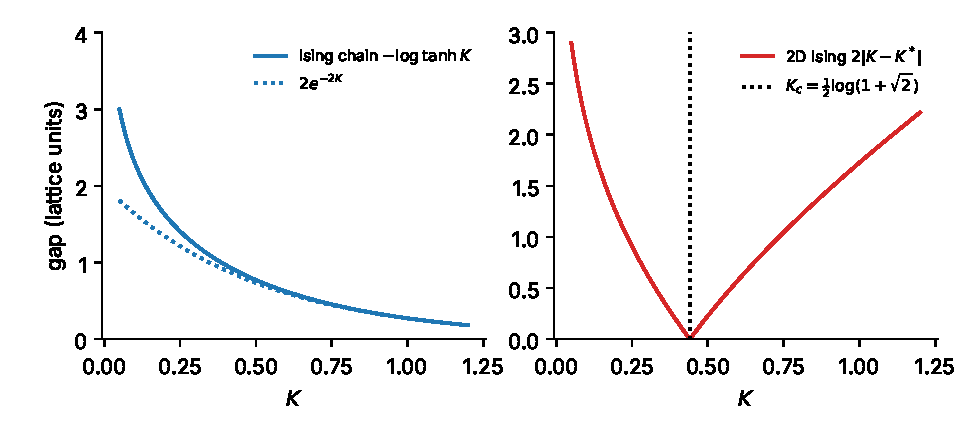
\includegraphics[width=\textwidth]{figures/examples_gaps.pdf}
\caption[Left: the Ising chain gap $-\log\tanh K$, positive for every finite $K$, closing only at zero]{Left: the Ising chain gap $-\log\tanh K$, positive for every finite $K$, closing only at zero temperature like $2e^{-2K}$. Right: the transfer matrix gap of the two dimensional Ising model, $2|K-K^*|$, which closes at the critical coupling; for $K>K_c$ the connected spin correlation decays at twice this rate.}
\label{fig:examplesgaps}
\end{figure}

Near $K_c$ the model has a continuum limit, the massive Ising field theory, obtained by letting the lattice spacing shrink like $|K-K_c|$. In those units the gap is again constant (for either of the two decay rates above), and the uniform Thorin gap inequality holds along that trajectory. At $K_c$ itself the continuum limit is the critical Ising field theory, a conformal field theory with no gap, and the Thorin densities decay polynomially as in the massless example.

\subsection{Lessons for Yang Mills}

The three examples sharpen what the Clay problem asks.
\begin{enumerate}
\item[(i)] In the two Ising examples a continuum limit exists, and the uniform Thorin gap inequality holds along it if and only if the correlation length in lattice units diverges no faster than the inverse lattice spacing. The inequality is not a property of a single lattice theory but of a trajectory.
\item[(ii)] In the Ising chain the continuum limit is reached at an endpoint of the coupling range, $K\to\infty$, and an exact renormalization map moves along the trajectory. Yang Mills is expected to behave this way, with $\beta\to\infty$ in place of $K\to\infty$ and asymptotic freedom fixing the rate. The Migdal Kadanoff ladder of Section~\ref{ch:mk} is the closest analogue in four dimensions.
\item[(iii)] In the two dimensional Ising model the continuum limit is reached at an interior critical point. Monte Carlo studies of lattice Yang Mills for SU(2)~\cite{Cr80} find no such transition in four dimensions, so the correlation length is expected to diverge only as $\beta\to\infty$. That is why the mass gap problem is a problem about the crossover between strong and weak coupling rather than about a critical point.
\item[(iv)] Absence of a gap shows up in Route A as a heavier than exponential tail of the GGC, and in Route B as polynomial decay of the Thorin densities. Both are detectable in principle, but by Proposition~\ref{prop:logconvex} data can only bound the gap from above, so a slowly decaying correlation can never be certified massless or massive by measurement alone.
\end{enumerate}

\section*{Exercises}
\begin{enumerate}
\item For $\mu_\alpha=w_1\delta_{m_1}+w_2\delta_{m_2}$, identify $X_\alpha$ as a sum of two independent gamma variables and verify Theorem~\ref{thm:abscissaB} directly.
\item Show that if $\mu$ has density $\rho(E)\sim c(E-\Delta)^\nu$ near $\Delta$, then $\Pr(X_\alpha>x)=e^{-\Delta x+o(x)}$, the full limit and not only the liminf of the corollary, by splitting off the part of $\mu_\alpha$ in $[\Delta,\Delta+\varepsilon]$ as an independent gamma convolution.
\item Show that the Yang Mills GGC of a direct sum of two independent sectors is the convolution of their GGCs, and that its gap is the minimum of the two gaps.
\item Use Bondesson's shot noise representation (the jumps $Y_j$ of a gamma process, intensity $y^{-1}e^{-y}\mathrm dy$, each divided by a rate $E_j$, the pairs $(E_j,Y_j)$ forming the Poisson process of Section~\ref{sec:routeAmain} with intensity $\mu_\alpha(\mathrm dE)\,y^{-1}e^{-y}\mathrm dy$) to write a simulation algorithm for $X_\alpha$ when $\mu_\alpha$ has an atomic part and a continuous part, and implement it for the toy spectrum of Figure~\ref{fig:routeAtail}.
\item Verify the two integrals used in the proof of Lemma~\ref{lem:2sin2B} (Section~\ref{ch:routeB}).
\item For $\mu=\delta_m$ compute $T_\alpha(z)$ explicitly and check Theorem~\ref{thm:rateB} by hand.
\item Show that $\psi_\alpha(t)/C(\alpha)$ is the L\'evy exponent of a compound Poisson process with unit jump rate, and interpret it as $1-\operatorname{Re}\varphi(t)$ for a characteristic function $\varphi$.
\item Prove that the uniform Thorin gap inequality with some constant $M$ implies it with $M=1$, without passing through the support of the spectral measures, by combining the inequality with the log convexity of $\alpha\mapsto T_\alpha(z)$ (Theorem~\ref{thm:rateB}(iii)); iterating the inequality alone only gives $M^n$.
\item Give a spectrum with two atoms for which the normalised correlation is not a GGC, and compute the location of the negative Thorin atom.
\item (Section~\ref{ch:examples}) Derive $\tanh K'=(\tanh K)^2$ for the Ising chain by summing out every other spin.
\item Show that the Ising chain correlation length in units of a lattice spacing $a(K)=e^{-2K}$ tends to a constant as $K\to\infty$.
\item (Section~\ref{ch:examples}) For the massless spectrum $E^{\kappa-1}\mathrm dE/\Gamma(\kappa)$, show that the Route A GGC has $\E e^{\lambda X_\alpha}=\infty$ for every $\lambda>0$.
\item Verify the closed form of $T_\alpha(z)$ for the massless spectrum and show that its local rate behaves like $(\kappa+2)/\alpha$.
\end{enumerate}

\chapter{Estimating the Gap}\label{ch:estimation}

Chapter~\ref{ch:routeA} turned the gap into a property of a positive measure. This chapter treats it as a parameter to be estimated from data, which is how lattice gauge theory meets it in practice. The main point is simple and underused: the spectral measure\index{spectral measure} itself is poorly determined by a noisy correlator, but the left edge of its support is well determined. The first sections develop the support constrained profile estimator and test it on a toy spectrum. The remaining three sections treat Monte Carlo methods from Bayesian computation that bear on estimation in lattice gauge theory: latent variable samplers and nested sampling (Section~\ref{ch:latent}), the vertical likelihood and split sampling (Section~\ref{ch:vertical}), and weighted Monte Carlo with the Yakowitz rate (Section~\ref{ch:yakowitz}).

\section{The inverse Laplace problem}

A lattice simulation produces estimates $y_i$ of $C(\tau_i)$ at a finite set of Euclidean times, with a covariance matrix estimated from the Monte Carlo samples. Recovering $\mu$ from $y$ means inverting the Laplace transform, one of the most ill conditioned problems in applied mathematics. The singular values of the Laplace operator restricted to a finite interval decay geometrically, so information about $\mu$ at fine resolution is lost exponentially fast in the noise. Very different measures can have Laplace transforms that agree to within any reasonable statistical error on a finite window.

In lattice QCD the problem goes by the name of spectral reconstruction, and the standard methods are the Backus Gilbert method~\cite{BG68}, maximum entropy, and the smeared spectral density approach of Hansen, Lupo and Tantalo \cite{HLT}, which targets $\mu$ convolved with a chosen kernel rather than $\mu$ itself. All of these accept that $\mu$ cannot be resolved pointwise.

\section{Positivity as the prior}

The Thorin viewpoint suggests a different emphasis. We know two things about $\mu$ with certainty: it is nonnegative, and it is supported on $[\Delta,\infty)$. The first is a constraint; the second is the quantity of interest. This is exactly the setting of positive linear inverse problems.

\begin{definition}
Given a grid $E_1<\dots<E_J$ and the kernel $K_{ij}=e^{-\tau_iE_j}$, the positive deconvolution\index{positive deconvolution} problem is to find $\nu\in[0,\infty)^J$ with $K\nu\approx y$.
\end{definition}

Vardi and Lee\index{Vardi, Y.!and Lee, D.}'s EM algorithm \cite{VL},
\[
\nu_j\leftarrow\nu_j\,\frac{\sum_iK_{ij}\,y_i/(K\nu)_i}{\sum_iK_{ij}},
\]
keeps $\nu$ positive at every step and decreases a Kullback Leibler divergence. Polson and Robert \cite{PR} interpreted the same iteration as a Monte Carlo inversion in the spirit of von Neumann, which opens the door to sampling based uncertainty quantification. Padilla, Polson and Scott \cite{PPS} give a Bayesian nonparametric treatment of deconvolution with guarantees on posterior contraction, and proximal methods, surveyed by Polson, Scott and Willard \cite{PSW15}, accelerate the fitting.

\section{The support constrained profile}

The new ingredient is to treat the gap as an explicit parameter.

\begin{definition}
For a candidate gap $\delta$, let
\[
\chi^2(\delta)=\min\Big\{(y-K\nu)^\top\Sigma^{-1}(y-K\nu):\ \nu\ge0,\ \nu_j=0\text{ for }E_j<\delta\Big\}.
\]
\end{definition}

The function $\chi^2(\delta)$ is nondecreasing in $\delta$, since raising $\delta$ shrinks the feasible set. As long as $\delta$ is below the true gap, the constrained fit can match the data as well as the unconstrained one. As soon as $\delta$ passes the true gap, the fit must replace the lightest state by heavier ones, whose Laplace transforms decay faster, and the misfit at large $\tau$ grows sharply. A natural estimate is
\[
\hat\Delta=\min\{\delta:\chi^2(\delta)-\chi^2_{\min}>c\}
\]
for a threshold $c$, with $c=4$ a convenient default. Each $\chi^2(\delta)$ is a nonnegative least squares problem, solved exactly by the Lawson and Hanson~\cite{LH74} algorithm.

\section{A worked example}

We used the toy spectrum of Chapter~\ref{ch:routeA}: stable states at $E=1,1.5,1.9$ with weights $1,0.6,0.3$, and a two particle continuum from $E=2$ with density $0.4\sqrt{E-2}\,e^{-0.3(E-2)}$. The correlation was computed at $\tau=0.1,0.2,\dots,6$, and independent Gaussian noise with standard deviation $0.2\%$ of each value was added.

Figure~\ref{fig:deconvB} shows the result. On the left, the EM reconstruction smears the three atoms into a broad bump, as any inverse Laplace method must at this noise level. On the right, the profile $\chi^2(\delta)$ is flat for $\delta<1$ and rises by many orders of magnitude just past $\delta=1$. The estimate is $\hat\Delta=1.02$, on a candidate grid with spacing $0.02$ (the table below uses spacing $0.01$).

\begin{figure}[t]
\centering
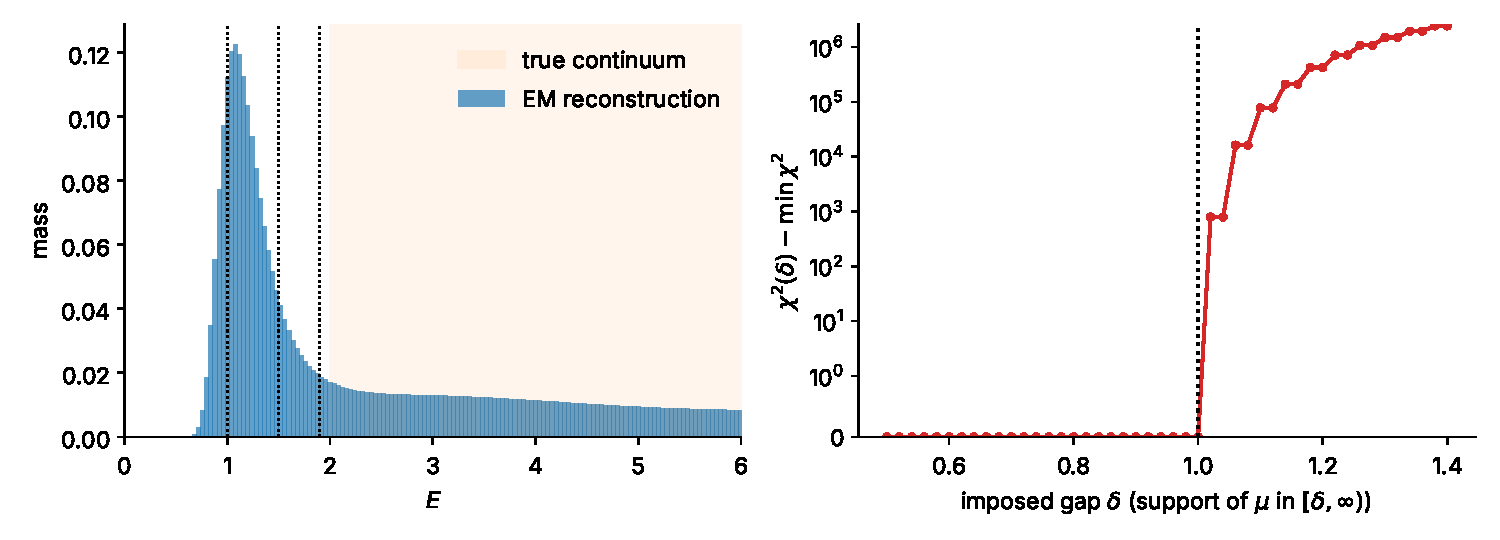
\includegraphics[width=\textwidth]{figures/deconvolution_gap.pdf}
\caption[Left: Vardi and Lee EM reconstruction of the spectral measure from a noisy correlator; dotted lines]{Left: Vardi and Lee EM reconstruction of the spectral measure from a noisy correlator; dotted lines mark the true atoms. Right: the support constrained profile $\chi^2(\delta)$ locates the gap sharply even though the measure itself is smeared.}
\label{fig:deconvB}
\end{figure}

Repeating the experiment twenty times at each noise level gave the following estimates, on a grid of candidate gaps with spacing $0.01$ and an energy grid with spacing $0.04$ (script \texttt{code/gap\_noise\_table.py}).
\begin{center}
\begin{tabular}{rccc}
\toprule
relative noise & mean $\hat\Delta$ & standard deviation & range \\ \midrule
0.1\% & 1.010 & 0.000 & 1.010 \\
0.5\% & 1.010 & 0.000 & 1.010 \\
1.0\% & 1.010 & 0.000 & 1.010 \\
2.0\% & 1.016 & 0.014 & 1.010 to 1.050 \\
\bottomrule
\end{tabular}
\end{center}
The estimate is pinned at the first candidate above the energy grid point $E=1$ up to one percent noise, so in this experiment the energy grid, not the noise, limits the resolution. At two percent noise the estimate begins to drift upward. Noise can only delay the rejection of a candidate above the true gap, so the estimate errs on the side of a larger gap, in line with the general lesson that data bound the gap from above.

\section{A Bayesian formulation}

The profile is the frequentist face of a simple hierarchical model. Put a prior $\pi(\delta)$ on the gap, and given $\delta$ a prior on positive measures supported on $[\delta,\infty)$, for instance a gamma process or a finite mixture with a sparsity prior on the weights. The likelihood is Gaussian in $y$. The marginal posterior of $\delta$ integrates the measure out, and EM or a proximal algorithm computes the conditional mode of the measure at each $\delta$. A Laplace approximation to the integral gives
\[
\log p(\delta\mid y)\approx-\tfrac12\chi^2(\delta)+\log\pi(\delta)+\log p(\hat\nu_\delta\mid\delta)+\tfrac{d_\delta}{2}\log2\pi-\tfrac12\log\det\mathcal I(\delta)+\text{const},
\]
where $\hat\nu_\delta$ is the constrained fit, $d_\delta$ the number of its nonzero components, and $\mathcal I(\delta)$ the observed information on them. Horseshoe type priors~\cite{CPS10} on the weights, which shrink small atoms hard while leaving large ones alone, are natural here: the spectrum of a gauge theory has a few stable states and a continuum, which is a sparse signal plus a smooth background.

\section{What estimation can and cannot do}

Local rates and the profile estimate both err toward a larger gap, so data bound the gap from above. Estimation can expose a wrong claim about the spectrum and measure a lattice gap precisely; it cannot prove that a gap exists or reach the continuum. Its role for the Clay problem is diagnostic: any proof strategy predicts lattice gaps at intermediate couplings, and those predictions can be tested with the methods of this chapter. The Migdal Kadanoff ladder of Section~\ref{ch:mk} makes such predictions.

\section{Latent Variables and Nested Sampling}\label{ch:latent}

Two families of Monte Carlo methods from Bayesian computation bear directly on lattice gauge theory: latent variable (auxiliary variable) Markov chain Monte Carlo, in the line of Swendsen and Wang\index{Swendsen, R. H.!and Wang, J. S.} \cite{SW87}, Edwards and Sokal \cite{ES88}, Besag and Green \cite{BG93}, and Higdon\index{Higdon, D.} \cite{Hi98}, together with slice sampling\index{slice sampling}, the Birge and Polson optimisation by slice sampling \cite{BP}, and Polson's 1996 embedding of a Cauchy likelihood in a log concave posterior \cite{Po96}; and Skilling's nested sampling\index{nested sampling} \cite{Sk06}, which Murray, MacKay, Ghahramani and Skilling applied to Potts models \cite{MMGS}. This section asks whether they are useful for the mass gap. The answer is yes in two ways and possibly in a third: as samplers for the lattice measures from which gaps are estimated, as a way of computing partition functions at every coupling at once, and, possibly, as a source of the common probability space that the comparison problem of Chapter~\ref{ch:path} needs.

\subsection{The heat bath is a latent variable method}

For SU(2), write a link as a unit quaternion $U\in S^3$. With all other links fixed, the Wilson action depends on $U$ only through the sum $A$ of the staples that complete its plaquettes (six in four dimensions, two in two), and a sum of SU(2) elements is a nonnegative multiple of an SU(2) element, $A=kV$. The conditional law of $U$ is therefore
\[
p(U\mid\text{rest})\propto\exp\big(\beta k\,\langle U,V^{-1}\rangle\big),
\]
a von Mises Fisher\index{von Mises Fisher law} law on $S^3$ with mean direction $V^{-1}$ and concentration $\beta k$. Creutz's heat bath \cite{Cr80} samples it exactly: writing $UV=a_0+i\sum_{j=1}^3a_j\sigma_j$, the component $a_0$ has density proportional to $\sqrt{1-a_0^2}\,e^{\beta ka_0}$ on $[-1,1]$, and the remaining direction is uniform on a two sphere.

Slice sampling makes the latent structure explicit. Introduce $u\mid a_0\sim\mathrm{Uniform}(0,e^{\beta ka_0})$. Then $a_0\mid u$ is distributed as $\sqrt{1-a_0^2}$ restricted to $a_0>\log u/(\beta k)$, which is easy to sample. The Kennedy and Pendleton algorithm \cite{KP85}, the standard SU(2) heat bath at weak coupling, is a rejection scheme of the same kind. These are instances of Higdon's general auxiliary variable framework, in which a latent variable makes the conditional of the original variable simple. Polson's 1996 construction, embedding a heavy tailed Cauchy likelihood in a log concave posterior through latent scale variables, is the same device used to restore log concavity.

\subsection{Swendsen and Wang, Edwards and Sokal, and partial decoupling\index{partial decoupling}}

For the Ising and Potts models the decisive latent variable method is the Swendsen and Wang algorithm. Each bond receives a latent indicator that is switched on with probability $1-e^{-\beta}$ when its two spins agree (the Potts convention, with weight $e^{\beta\delta_{\sigma_i\sigma_j}}$); given the bonds, clusters of connected spins are recoloured independently. Edwards and Sokal identified the joint law of spins and bonds, whose bond marginal is the Fortuin and Kasteleyn~\cite{FK72} random cluster model. The method reduces critical slowing down because a single update can flip clusters of any size.

Higdon's 1998 paper generalised this to partial decoupling: the latent bonds absorb only a fraction of each interaction, so that clusters are smaller but the remaining interactions keep the image model faithful. Partial decoupling trades mixing speed against fidelity in a controlled way, and it applies to models, like spatial image priors, for which full decoupling gives clusters that are too large to be useful.

For gauge theories the picture is less favourable. Cluster constructions have been proposed for $\Z_2$ lattice gauge theory and some abelian models, but we know of no efficient cluster algorithm for SU(N) lattice gauge theory. The obstruction is the one met throughout this book: no Fortuin Kasteleyn representation is known with the monotonicity that makes clusters percolate in step with the physics, and no FKG inequality is known for nonabelian link variables. Partial decoupling in Higdon's sense remains a plausible way to reduce autocorrelations, for example by decoupling the abelian part of each plaquette interaction, but we do not know of a version for SU(N) that has been shown to help.

\subsection{The character expansion as a latent variable model}

There is a second, exact latent variable representation of every lattice gauge theory, and it connects directly to positivity. Expand each plaquette weight in characters, $f(U_p)=\sum_nn\,c_n\chi_n(U_p)$, and introduce a latent label $n_p$ for each plaquette. The joint weight of links and labels is
\[
\prod_p n_p\,c_{n_p}\,\chi_{n_p}(U_p).
\]
Integrating out the links with Haar measure forces the labelled plaquettes to form closed surfaces with compatible labels, giving a sum over decorated surfaces; this is the strong coupling expansion of Chapter~\ref{ch:strong}, and the surface sums studied by Chatterjee \cite{Ch19so,Ch19} and others. The label weights $n_pc_{n_p}$ are nonnegative exactly when $c_n\ge0$, which is the Osterwalder Seiler~\cite{OSe} sufficient condition for reflection positivity (Chapter~\ref{ch:positivity}). The characters $\chi_{n_p}(U_p)$ change sign, so the joint weight of links and labels is not itself nonnegative: the positivity is that of the label factors, and we do not claim that reflection positivity implies a positive latent representation.

Two consequences matter here. First, the Migdal Kadanoff step acts on the latent weights in a simple way: decimation raises the normalised coefficients $c_n$ (the label weights up to the factor $n$) to the power $b^2$, and bond moving combines labels by the Clebsch Gordan rule with nonnegative multiplicities (Lemma~\ref{lem:posB}). The renormalization ladder is a flow on the label weights, which are nonnegative when $c_n\ge0$. Second, worm and surface algorithms that sample the labels directly can be read as the dual, latent side of a Swendsen and Wang type scheme.

\subsection{Nested sampling}

Nested sampling, introduced by Skilling, computes the evidence $Z=\int L(x)\,\pi(\mathrm dx)$ by compressing the prior mass. It keeps $N$ live points drawn from the prior subject to $L>L^*$, repeatedly discards the point with the lowest likelihood, raises the threshold $L^*$ to its value, and replaces it by a new point drawn from the prior subject to the new threshold. After $i$ steps the prior mass $X_i$ above the threshold satisfies $\E\log X_i=-i/N$, and
\[
Z\approx\sum_i(X_{i-1}-X_i)\,L_i .
\]
The shrinkage factors $X_i/X_{i-1}$ are independent Beta$(N,1)$ variables, so $-\log X_i$ is a sum of independent exponential variables with mean $1/N$: the compression is a Poisson process in $-\log X$. Nested sampling is thus a first passage construction of the same kind as the renormalization walk of Section~\ref{ch:verification}, with the likelihood threshold playing the role of the coupling.

Murray, MacKay, Ghahramani and Skilling applied nested sampling to Potts models and showed two things that matter for gauge theory. Because the sampler works with likelihood contours rather than temperatures, it is not trapped by first order phase transitions, where thermodynamic integration and tempering fail. And one run gives the partition function at every temperature, since the dead points and their prior masses estimate the whole density of states\index{density of states}. Polson and Scott's vertical likelihood Monte Carlo \cite{PSvl} makes the same idea, integrating over likelihood levels rather than parameter space, the basis of a general estimator (Section~\ref{ch:vertical}).

\subsection{The density of states and Bernstein in the coupling}

For SU(2) lattice gauge theory take the prior to be the Haar measure on all links and the likelihood $e^{-\beta S}$ with $S=\sum_p(1-\frac12\operatorname{tr}U_p)\ge0$. Nested sampling records the action thresholds $S_i$ and prior masses $X_i$, which estimate the density of states $\rho$ of the action under Haar measure, and then
\[
Z(\beta)=\int_0^\infty e^{-\beta S}\,\rho(S)\,\mathrm dS
\]
for every $\beta$ at once. This formula is a Laplace transform of a nonnegative measure, so $Z$ is completely monotone in the coupling. The spectral measure of Chapters~\ref{ch:positivity} and~\ref{ch:routeA}, a measure on energies indexed by Euclidean time, has a counterpart here, a measure on actions indexed by the coupling, and complete monotonicity, the starting point of the Thorin machinery, holds for it. Its support reaches down to $S=0$, the pure gauge configurations, so there is no gap in $\beta$: as in the massless example of Section~\ref{ch:examples}, $Z(\beta)$ decays polynomially as $\beta\to\infty$, with an exponent set by the number of fluctuating modes. Density of states methods are established in lattice gauge theory, for example the linear logarithmic relaxation method of Langfeld, Lucini and Rago \cite{LLR}; nested sampling is a Bayesian route to the same object, with built in error estimates.

\subsection{A test with an exact answer}

Two dimensional lattice gauge theory gives an exact check. On an $m\times m$ torus with $P=m^2$ plaquettes and Haar normalised links, the character expansion gives
\[
Z(\beta)=e^{-\beta P}\sum_{n\ge1}c_n(\beta)^P,\qquad c_n(\beta)=\frac{2I_n(\beta)}{\beta},
\]
because the torus has Euler characteristic zero. We ran nested sampling for SU(2) on a $3\times3$ torus, with $200$ live points and replacement by a constrained random walk on single links with adaptive step size, for $6490$ iterations, until the action threshold fell to $0.6$, a compression of the prior by a factor $e^{-32.5}$. A plain Monte Carlo average over $20{,}000$ Haar configurations at $\beta=1$ gives $\log Z(1)=-7.8970$ against the exact $-7.8975$, confirming the formula.

\begin{figure}[t]
\centering
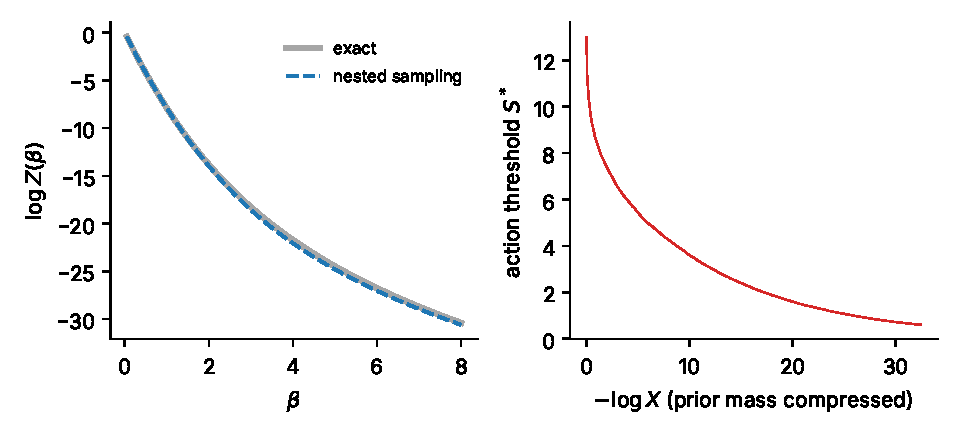
\includegraphics[width=\textwidth]{figures/nested_su2.pdf}
\caption[Nested sampling for two dimensional SU(2) on a $3\times3$ torus]{Nested sampling for two dimensional SU(2) lattice gauge theory on a $3\times3$ torus. Left: $\log Z(\beta)$ from a single run, against the exact character formula, for all $\beta$ in $[0.05,8]$. Right: the action threshold against the compression $-\log X$; it is the inverse cumulative density of states of the action under Haar measure.}
\label{fig:nested}
\end{figure}

The single run reproduces $\log Z(\beta)$ over the whole range $\beta\in[0.05,8]$ (Figure~\ref{fig:nested}; script \texttt{code/nested\_su2.py}), with largest error $0.35$, near $\beta\approx4$ ($0.20$ at $\beta=8$). That is the size expected from Skilling's estimate \cite{Sk06} $\sqrt{H/N}$ of the standard error of $\log Z$, since reaching the posterior at $\beta=8$ requires an information $H$ of about eighteen nats; more live points shrink it at the usual Monte Carlo rate. The test is small, but it shows the two features that matter: one run serves all couplings, and the output is a positive measure whose Laplace transform is the partition function.

\subsection{Are these methods useful for the mass gap?}

For estimation, yes. Measuring lattice gaps near the continuum limit is limited by autocorrelation, and in four dimensions above all by the freezing of topological charge as the lattice spacing shrinks. Methods that move along likelihood contours, such as nested sampling, or that act on large latent structures, such as cluster and worm algorithms, are the natural candidates for multimodal and slowly mixing targets. The support constrained gap estimator of this chapter needs correlators at large Euclidean times, which is where better samplers pay off.

For the renormalization ladder, yes. The heat kernel projection of Section~\ref{ch:verification} replaces each effective plaquette law by a one parameter family. Nested sampling on a single Migdal Kadanoff block, or on a small block of the true lattice, computes the full effective partition function as a function of the coupling, which is the input needed to test the projection, to follow the flow without truncation, and to compare the Migdal Kadanoff block with a true block.

For the proof, possibly, and this is the most interesting point. The comparison problem of Chapter~\ref{ch:path} asks for a true block spin step and a Migdal Kadanoff step on a common probability space, compared in the likelihood ratio order. Latent variable constructions are exactly how such common spaces are built. The monotonicity of the random cluster model (the FKG and comparison inequalities) belongs to the model of Fortuin and Kasteleyn itself, and the Edwards and Sokal joint representation is what carries the random cluster results, including coupling proofs of exponential decay, over to the Potts model. Higdon's partial decoupling interpolates between the original model and a decoupled one, which is the kind of interpolation a sandwich needs. The label weights of the character expansion are nonnegative when $c_n\ge0$, which supplies positivity for the label factors only. What it does not supply is a monotone coupling: without an FKG inequality for nonabelian link variables, the clusters or surfaces of one theory need not dominate those of the other. Finding a latent representation of SU(N) gauge theory with the right monotonicity, perhaps one built from the Biane Pitman Yor variables \cite{BPY} that carry the curvature, would be a genuine step on the open problem of Chapter~\ref{ch:path}.

\section{Vertical Likelihood and Split Sampling}\label{ch:vertical}\index{vertical likelihood}\index{split sampling}\index{Polson, N. G.!and Scott, J. G.}

The partition function of a lattice gauge theory is a normalising constant. Every method for computing normalising constants in Bayesian statistics therefore has a lattice counterpart, and the vertical likelihood perspective of Polson and Scott \cite{PSvl} organises the most important of them under one principle. This section lists the methods it unifies, adds split sampling, implements all of them on a lattice gauge theory with an exact answer, and asks which are useful for the mass gap.

\subsection{The vertical representation}

Let $\pi$ be a probability measure, the prior, and $L\ge0$ a likelihood, with $Z=\int L\,\mathrm d\pi$. Polson and Scott build everything from two functions: the upper tail function of the likelihood ordinate,
\[
T(y)=\pi\{x:L(x)>y\},
\]
the prior mass above level $y$, and its pseudo inverse $\ell(s)=\sup\{y:T(y)>s\}$. Interchanging the order of integration gives two one dimensional identities,
\[
Z=\int_0^\infty T(y)\,\mathrm dy=\int_0^1\ell(s)\,\mathrm ds .
\]
The integral over the original space, of any dimension, collapses onto the line of likelihood ordinates. This is the vertical view: instead of integrating across the space horizontally, integrate up the likelihood.

For lattice gauge theory the prior is Haar measure on the links, the likelihood is $e^{-\beta S}$, and the level sets $\{L>y\}$ are the action sublevel sets $\{S<s\}$. Then $T(y)$ is the prior mass $X(s)$ of configurations with action below $s$, the cumulative density of states, and
\[
Z(\beta)=\int_0^\infty e^{-\beta s}\,\mathrm dX(s),
\]
the Laplace transform in the coupling of the density of states introduced in Section~\ref{ch:latent}.

\subsection{The vertical likelihood principle}

The one dimensional identities are not to be used by direct quadrature: $T(y)$ changes far too quickly near the top of the likelihood. Polson and Scott use them instead to design importance functions. Choose a weight function $w\ge0$ on likelihood ordinates with cumulative $W(u)=\int_0^uw$ (where $w$ may carry an atom at $0$, so that $W(0)>0$), and form the joint law
\[
\pi_w(x,u)\propto w(u)\,\mathrm{I}\{0<u<L(x)\}\,\pi(x),
\]
whose $x$ marginal is $\pi_w(x)\propto\pi(x)W(L(x))$. Sampling $x$ from $\pi_w$ and taking the ratio of the means of $L/W$ and $1/W$ estimates $Z$. The design problem, which in ordinary importance sampling is the choice of a proposal over a high dimensional space, is reduced to the choice of a one dimensional weight function on the likelihood ordinate.

\begin{theorem}[Polson and Scott \cite{PSvl}]
If $T(y)$ is differentiable and $\xi\sim\pi_w$, the likelihood ordinate $Y=L(\xi)$ has density $f(y)=-W(y)T'(y)/Z_w$, where $Z_w=\int W(L)\,\mathrm d\pi$.
\end{theorem}
\begin{proof}
Under $\pi$ the ordinate $Y=L(\xi)$ has survival function $T(y)$, hence density $-T'(y)$. The $x$ marginal $\pi_w$ reweights $\pi$ by $W(L(x))/Z_w$, so the ordinate density is $W(y)(-T'(y))/Z_w$.
\end{proof}

The score function heuristic asks that the ordinate density be proportional to $-T'(y)/T(y)$, concentrating samples where the tail function changes fastest relative to its size, since that is where the integral $\int T(y)\mathrm dy$ is decided. The theorem then says to take $W(u)=1/T(u)$, and the default weight is the truncated version
\[
W(u)=\frac{1}{\max\{\eta,T(u)\}},\qquad 0<\eta\le1 .
\]
Sampling from $\pi_w$ is done by weighted slice sampling, alternating $u\mid x$ from $w$ truncated to $(0,L(x))$ and $x\mid u$ from the prior truncated to $\{L(x)>u\}$.

\subsection{The methods it unifies}

Polson and Scott \cite{PSvl} show that seven classes of methods are special cases or close relatives, distinguished by the weight function.
\begin{enumerate}
\item Importance sampling, with any proposal, implies some law of the ordinate; the vertical view chooses that law directly.
\item Slice sampling: the uniform weight $w\equiv1$ recovers the ordinary slice sampler conditionals, whose target is the posterior.
\item Annealing and tempering: $w(u)=au^{a-1}$ gives $W(u)=u^a$ and the power posterior $p\,L^a$ of Friel and Pettitt~\cite{FP08}, the basis of simulated and annealed importance sampling; adding a point mass at zero gives bridge and path sampling.
\item The harmonic mean estimator: with $w\equiv1$ the weights are $1/L$, which is the Newton and Raftery~\cite{NR94} estimator, with its well documented infinite variance.
\item Troutt's vertical density sampler~\cite{Tr91}, of which the theorem above is a generalisation.
\item Energy level sampling from statistical physics: $W=1/\rho(s)$, with $\rho$ the density of states of Section~\ref{ch:latent}, gives multicanonical sampling and the Wang and Landau~\cite{WL01} algorithm, and $W=1/X(s)$, the untruncated default weight, the $1/k$ ensemble of Hesselbo and Stinchcombe~\cite{HS95}.
\item Nested sampling, which Polson and Scott show sequentially constructs an importance function close to the default score function weight.
\end{enumerate}

\subsection{Split sampling and optimisation by slicing}

Split sampling, which we take from unpublished work of Birge, Chang and Polson, estimates expectations and rare event probabilities in high dimensions. It splits the quantity of interest into an integrated family of normalisation constants indexed by an auxiliary level variable, runs an MCMC on the joint space of state and level, and adapts weights on the levels, in the manner of Wang and Landau, so that every level is visited. The marginal occupation of the levels then estimates the rare event probabilities $X(s_t)$ at the level values $s_t$, and the expectation is assembled from them. For likelihood level sets this is a discrete version of the vertical identity, with the levels chosen adaptively. Birge and Polson's optimisation by slice sampling \cite{BP} uses the same auxiliary variable construction to locate maxima: the slice variable pushes the chain up the likelihood, and in the limit of a sharpening weight it concentrates on the mode.

For gauge theory, both ideas fit naturally. The rare events are configurations of low action, or of nontrivial topology, which a standard Markov chain rarely visits at weak coupling. Split sampling across action levels or across topological sectors is a principled way to visit them, and optimisation by slicing locates the classical minima of the action, around which the weak coupling expansion is built.

\subsection{An implementation with an exact answer}

We implemented the methods on two dimensional SU(2) lattice gauge theory on a $3\times3$ torus, where $\log Z(2)=-13.8223$ exactly from the character formula of Section~\ref{ch:latent}. Each method received about $2.4\times10^5$ single link updates of its own (the harmonic mean about half that); the vertical likelihood sampler and split sampling also reuse the nested sampling run as a pilot, so their total cost is about twice that of the others. The posterior kernel throughout is the slice sampling heat bath of Section~\ref{ch:latent}, which reproduces the exact posterior mean action, $5.10$ at $\beta=2$, to within Monte Carlo error. The vertical likelihood sampler uses the default weight with $X(s)$ estimated by a pilot nested run, and split sampling uses thirteen action levels spaced evenly in $\log X$ down to $e^{-14}$, with Wang and Landau adaptation of the level weights. Three independent seeds (5, 11 and 23) give the following root mean square errors in $\log Z(2)$, each taken over the three seeds. The script \texttt{code/vl\_methods.py} saves the per seed results in \texttt{results/}, and \texttt{code/book\_figs4.py} builds the table and the figure from them.

\begin{center}
\footnotesize
\resizebox{\textwidth}{!}{\begin{tabular}{lcc}
\toprule
method & weight $W(u)$ & RMSE \\ \midrule
prior importance sampling & $1$ & 0.117 \\
harmonic mean & $u$ & 0.275 \\
power posterior path sampling & $u^a$ ladder & 0.057 \\
nested sampling & sequential, near $1/T(u)$ & 0.218 \\
vertical likelihood, Metropolis on $\pi_w$ & $1/\max\{\eta,T(u)\}$ & 0.032 \\
split sampling & adaptive on levels & 0.140 \\
Wang and Landau & $1/\rho(s)$ & not converged \\
\bottomrule
\end{tabular}}
\end{center}

\begin{figure}[t]
\centering
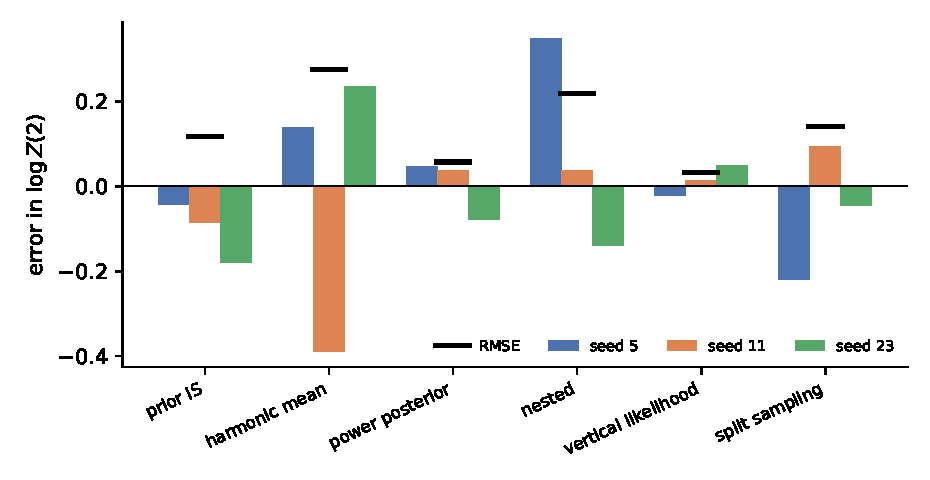
\includegraphics[width=\textwidth]{figures/vl_errors.pdf}
\caption[Errors of the vertical likelihood family on two dimensional SU(2)]{Errors in $\log Z(2)$ for five members of the vertical likelihood family and split sampling on the $3\times3$ SU(2) torus, three seeds each, with the root mean square error marked. The harmonic mean has the largest errors and no stable sign, as its infinite variance theory predicts.}
\label{fig:vlerrors}
\end{figure}

Three lessons stand out. First, the harmonic mean is the least accurate and its error changes sign between seeds ($+0.14$, $-0.39$, $+0.24$), as its infinite variance theory predicts. Second, the vertical likelihood sampler has the smallest error here ($0.032$), followed by power posterior path sampling ($0.057$), while plain importance sampling from the prior ($0.117$) is already competitive with split and nested sampling on this small problem with a modest likelihood. With three seeds the order of the closer methods is not established. Polson and Scott report that on sharper likelihoods, as in their fifty dimensional example, weighted slice sampling beats nested sampling by a wide margin \cite{PSvl}. Third, Wang and Landau did not converge within the common budget: the flat histogram condition was not met in the rarely visited energy bins, and anchoring an unconverged density of states produces large errors. Adaptive energy level methods need budgets far beyond those of the other methods.

\begin{figure}[t]
\centering
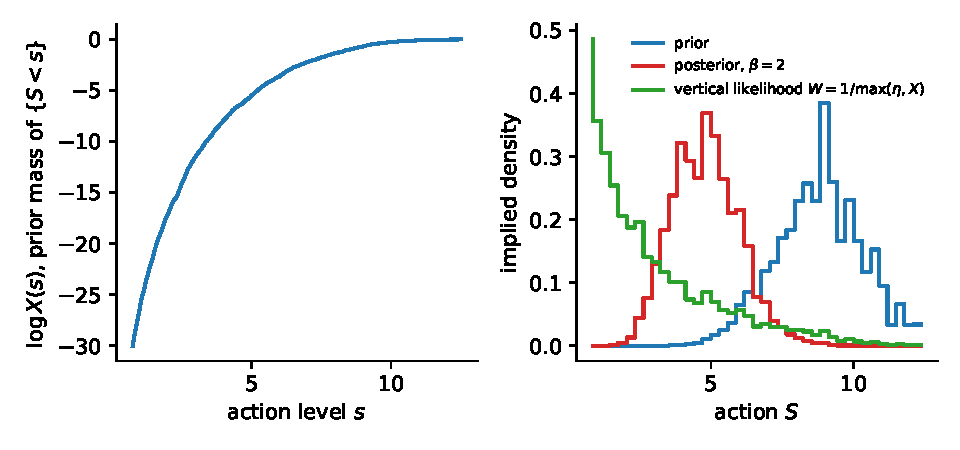
\includegraphics[width=\textwidth]{figures/vl_implied.pdf}
\caption[Implied laws of the action under three weight functions]{Left: the prior mass $X(s)$ of $\{S<s\}$ from a nested run, the cumulative density of states. Right: the implied law of the action under the prior, under the posterior at $\beta=2$, and under the default vertical likelihood weight, which spreads samples across all action levels.}
\label{fig:vlimplied}
\end{figure}

\subsection{Are vertical likelihood methods useful for the gap?}

Yes, for the reasons given for nested sampling in Section~\ref{ch:latent}, and for two more. The score function heuristic is the right principle for visiting the rare, low action configurations that dominate at weak coupling, and split sampling by topological sector would be a natural attack on topological freezing, though we did not test it (the two dimensional torus has no topological sectors). The methods are also diagnostics for the renormalization ladder: the partition function of a single block, as a function of the coupling, determines the Migdal Kadanoff step, and vertical methods compute it without truncating the character expansion.

\section{Weighted Monte Carlo and the Yakowitz Rate}\label{ch:yakowitz}\index{Yakowitz, S.}\index{weighted Monte Carlo}\index{thermodynamic integration}

Many quantities in this book are one dimensional integrals evaluated at random points: thermodynamic integration over the coupling, the vertical identity over likelihood ordinates, Thorin densities over energies. For such integrals there is a simple and much underused improvement on plain Monte Carlo, due to Yakowitz, Krimmel and Szidarovszky \cite{Ya78}.

\subsection{The result}

Let $f$ be a function on $[0,1]$ and $U_{(1)}\le\dots\le U_{(n)}$ the order statistics of $n$ independent uniform variables, with $U_{(0)}=0$ and $U_{(n+1)}=1$. Plain Monte Carlo estimates $\int f$ by $\frac1n\sum f(U_i)$, with mean square error of order $n^{-1}$. Weighted Monte Carlo applies the trapezoid rule to the sorted points:
\[
\hat I_n=\sum_{i=0}^{n}\frac{f(U_{(i)})+f(U_{(i+1)})}{2}\,\big(U_{(i+1)}-U_{(i)}\big).
\]
They proposed this in 1978 and showed that it converges much faster than plain Monte Carlo for smooth integrands. Masry and Cambanis~\cite{MC90} made the rate precise: if $f$ has two continuous derivatives, the mean square error is of order $n^{-4}$, and they identified the constant; it is of exact order $n^{-4}$ when $f'(0)\ne f'(1)$, since the leading bias is $(f'(1)-f'(0))/(2n^2)$. The root mean square error is therefore of order $n^{-2}$ instead of $n^{-1/2}$.

The reason is simple. Conditional on the spacings, the trapezoid error is a sum of local errors of size $f''$ times the cube of each spacing. Uniform spacings behave like independent exponential variables divided by $n$, so each local error is of order $n^{-3}$. The local errors share the sign of $f''$ and do not cancel, so the sum is a bias of order $n\cdot n^{-3}=n^{-2}$, which gives the mean square error of order $n^{-4}$.

\subsection{A test on thermodynamic integration}

The log partition function of the two dimensional SU(2) torus is
\[
\log Z(2)=-\int_0^2\langle S\rangle_\gamma\,\mathrm d\gamma,
\]
where $\langle S\rangle_\gamma$ is the mean action at coupling $\gamma$. To isolate the quadrature error we evaluated $\langle S\rangle_\gamma$ exactly and placed $n$ rungs uniformly at random, comparing plain Monte Carlo with the trapezoid rule on the sorted rungs. Over three thousand repetitions the root mean square error fell like $n^{-0.50}$ for plain Monte Carlo and like $n^{-1.98}$ for the weighted rule, fitted on $n\ge16$ (Figure~\ref{fig:yak}; script \texttt{code/yakowitz\_ti.py}). At $256$ rungs the errors were $0.14$ and $2.4\times10^{-5}$, a factor of nearly six thousand.

\begin{figure}[t]
\centering
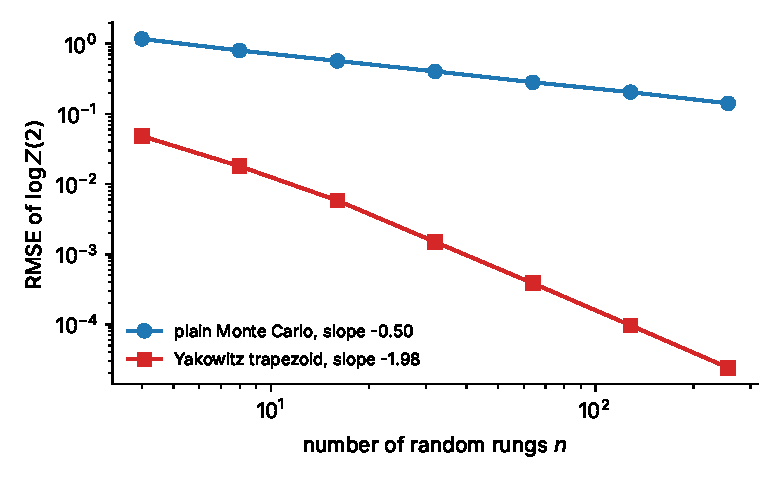
\includegraphics[width=0.85\textwidth]{figures/yakowitz_ti.pdf}
\caption[Yakowitz weighted Monte Carlo against plain Monte Carlo]{Root mean square error of $\log Z(2)$ by thermodynamic integration with $n$ random rungs. Plain Monte Carlo falls like $n^{-1/2}$; the trapezoid rule on the sorted rungs falls like $n^{-2}$, as the theory of Masry and Cambanis predicts.}
\label{fig:yak}
\end{figure}

A practical warning came out of the test. Our first run showed a rate of $n^{-1}$, not $n^{-2}$. The cause was a numerical defect in the integrand near $\gamma=0$, where a finite difference step crossed the origin. The weighted rule is only as good as the smoothness of the integrand, and a single jump costs a full order. This is useful in reverse: an observed rate below $n^{-2}$ is evidence of a jump in the integrand, which in thermodynamic integration means a first order phase transition or a numerical error.

\subsection{Where it helps, and where it does not}

The weighted rule helps whenever the random points are one dimensional and the integrand is smooth.
\begin{itemize}
\item Simulated tempering visits couplings at random. Sorting the visited couplings and applying the trapezoid rule to the measured mean actions gives a free energy with the Yakowitz rate in the quadrature, leaving only the Monte Carlo error of each mean.
\item Thorin densities and spectral integrals evaluated at sampled energies benefit in the same way.
\item The positive deconvolution above integrates a fitted measure against smooth kernels; sorted support points with trapezoid weights improve those integrals.
\end{itemize}
It does not help where the dominant error is not quadrature. In nested sampling the ordinates $X_i$ are not observed but estimated, with an error of order $\sqrt{H/N}$ in $\log Z$, and replacing rectangles by trapezoids in $X$ changed our estimates by only $0.005$ against a statistical error of $0.2$. Nor does it help in high dimensions directly: the rate rests on one dimensional spacings. The vertical identity of Section~\ref{ch:vertical} is what makes it relevant, by turning a high dimensional integral into a one dimensional one over likelihood ordinates or couplings.

\subsection{A connection with Euler Maclaurin}

The weighted rule is closely related to the sawtooth corrections in Stirling type expansions of $\log n!$ and to the Euler Maclaurin formula: the trapezoid rule on equally spaced points has error governed by Bernoulli numbers, and random spacings replace those constants by moments of exponential spacings.

\section*{Exercises}
\begin{enumerate}
\item Show that $\chi^2(\delta)$ is nondecreasing in $\delta$, and that the profile estimate $\hat\Delta$ is therefore well defined for any threshold $c$ for which the defining set is nonempty (this chapter, the support constrained profile).
\item Show that a sum of SU(2) elements is a nonnegative multiple of an SU(2) element, and derive the von Mises Fisher form of the link conditional. (Section~\ref{ch:latent})
\item Write out the slice sampler for $a_0$ with density proportional to $\sqrt{1-a_0^2}\,e^{\kappa a_0}$, and compare its acceptance with the Kennedy and Pendleton method for large $\kappa$. (Section~\ref{ch:latent})
\item Prove that the shrinkage factors in nested sampling are Beta$(N,1)$, and deduce that $-\log X_i$ is a sum of independent exponential variables with mean $1/N$. (Section~\ref{ch:latent})
\item Derive the torus formula $Z(\beta)=e^{-\beta P}\sum_nc_n(\beta)^P$ by integrating out links in the character expansion, and find the polynomial rate at which $Z(\beta)$ decays as $\beta\to\infty$. (Section~\ref{ch:latent})
\item Prove both identities $Z=\int_0^\infty T(y)\mathrm dy=\int_0^1\ell(s)\mathrm ds$. (Section~\ref{ch:vertical})
\item Show that $w\equiv1$ gives the harmonic mean estimator and explain its infinite variance in terms of the ordinate law. (Section~\ref{ch:vertical})
\item Show that $w(u)=au^{a-1}$ gives the power posterior, and derive the thermodynamic integration identity from it. (Section~\ref{ch:vertical})
\item For lattice gauge theory, write the default weight in terms of the density of states and explain why its importance function is independent of $\beta$. (Section~\ref{ch:vertical})
\item Show that uniform spacings have the law of independent exponential variables divided by their sum. (Section~\ref{ch:yakowitz})
\item Compute the mean square error of the weighted rule for $f(x)=x^2$ exactly and verify the $n^{-4}$ rate. (Section~\ref{ch:yakowitz})
\item Explain why the weighted rule with an integrand that has a jump has root mean square error of order $n^{-1}$, while a kink leaves the rate $n^{-2}$. (Section~\ref{ch:yakowitz})
\end{enumerate}

\chapter{Markov Chains, Mixing and Slice Variables}\label{ch:kac}\index{Kac, M.}\index{P\'olya, G.}\index{Ehrenfest urn}\index{Feynman Kac formula}

Chapter~\ref{ch:estimation} estimated the gap from simulated data. This chapter asks what limits the simulation itself: Markov chain Monte Carlo for gauge fields, how fast such chains mix and why, for spin systems, that is tied to the decay of correlations, the cluster and multigrid methods that attack critical slowing down, the topological freezing that they do not remove, and the slice variables that turn a hard conditional into a log concave one. It opens with Mark Kac's discussion of models, because the Feynman Kac formula~\cite{Ka49} and Kac's lemma on return times are the exact tools that reappear later. It then takes in turn Jerrum and Sinclair on randomised approximation and rapid mixing, Sokal on autocorrelation, clusters and zeros, and slice sampling with Besag's Markov random fields.

\section{Kac and the Use of Models}\label{sec:c5kac}

Mark Kac thought hard about what a mathematical model is for, and he often illustrated the point with problems that P\'olya had made famous: the random walk that returns home, the urn that refills itself. This section asks whether that discussion is useful for the mass gap. We think it is, at three levels: as a philosophy that justifies the Migdal Kadanoff caricature, as a set of exact results about recurrence and return times that reappear in renormalization and in Monte Carlo, and through the Feynman Kac formula, which is the bridge between the Euclidean measures of this book and the Hamiltonian whose gap we want.

\subsection{Models as caricatures}

In his 1969 essay \emph{Some Mathematical Models in Science}~\cite{Ka69}, Kac argued that the purpose of a model is not to be a faithful copy of reality but to isolate a mechanism so cleanly that its consequences can be computed, and then to ask which features of reality survive. A good model is a caricature: it exaggerates what matters and discards the rest. His own examples included the Ehrenfest urn, which explains how irreversible behaviour can arise from reversible dynamics, and the Kac ring, a deterministic model of the same paradox.

The Migdal Kadanoff ladder of Sections~\ref{ch:mk} and~\ref{ch:verification} is a caricature in exactly Kac's sense. It discards the true geometry of block spin transformations on $\Z^4$ and keeps two operations, a Bayesian product and a convolution, together with the curvature of the group. What survives is asymptotic freedom with a one loop coefficient within three percent of the truth at scale factor $b=2$ (an agreement specific to $b=2$), confinement at every coupling, and a correlation length that is a first passage time. Kac's view tells us how to use such a model: not as evidence that the real theory has a gap, but as a precise statement of which mechanism would produce one, and therefore of what must be compared to make the argument real. That is how Chapter~\ref{ch:path} is framed. P\'olya's own advice in \emph{How to Solve It}, to solve an auxiliary problem first and to specialise before generalising, is the strategy of Chapter~\ref{ch:twod} and Section~\ref{ch:mk}: solve two dimensions exactly, then a caricature of four.

\subsection{P\'olya's walk and marginal dimensions}\label{sec:c5polya}

P\'olya proved in 1921 that simple random walk on $\Z^d$ returns to its starting point with probability one when $d\le2$ and with probability less than one when $d\ge3$; in three dimensions the return probability is about $0.34$. Kac gave a celebrated exposition of this result and of its connection with Brownian motion. The proof turns on whether the expected number of returns, $\sum_n p_n(0,0)$ with $p_n(0,0)\asymp n^{-d/2}$ for even $n$, diverges.

\begin{figure}[t]
\centering
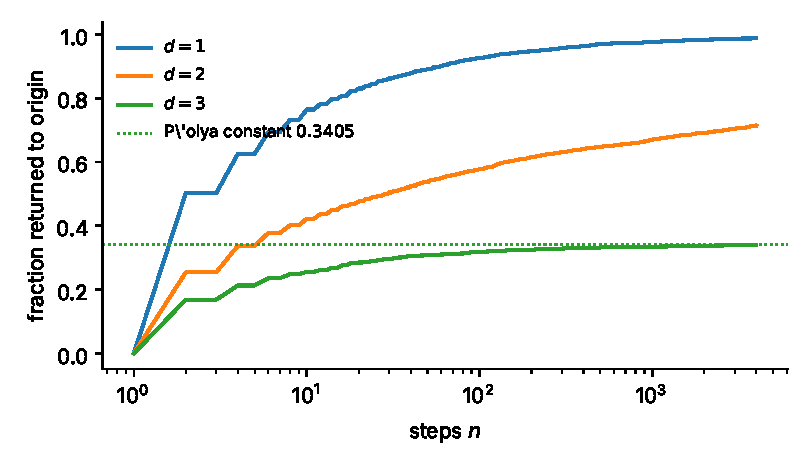
\includegraphics[width=0.85\textwidth]{figures/polya_walk.pdf}
\caption[P\'olya's random walk in one, two and three dimensions]{Fraction of four thousand random walkers that have returned to the origin by step $n$. In one dimension the fraction rises fastest; in two it is certain but logarithmically slow; in three it saturates near P\'olya's constant $0.3405$.}
\label{fig:polya}
\end{figure}

Two dimensions is the marginal case: return is certain, but the expected number of returns grows only like $\log n$, and the walk takes a logarithmically long time to make its point (Figure~\ref{fig:polya}). Four dimensional Yang Mills is the marginal case of the renormalization group in the same sense. The Gaussian ledger of Section~\ref{ch:mk} shows that in flat space the coupling neither grows nor shrinks, and the logarithmic running of asymptotic freedom is the analogue of the logarithmic accumulation of returns. The two cases are not alike in every respect. For the walk, the leading term $p_{2n}(0,0)\sim1/(\pi n)$ already makes the expected number of returns diverge, so recurrence is decided at leading order and the constant $1/\pi$ only sets the rate $\log n$ of that divergence. For Yang Mills the leading order is the neutral Gaussian ledger, and the answer is decided by a correction that is invisible there, the curvature of the group, carried by the Biane Pitman Yor variable.

\subsection{Kac's lemma and the Ehrenfest urn}\label{sec:c5kaclemma}

Kac's lemma says that for a stationary ergodic process, the mean return time to a set $A$ of positive measure, for the process started in $A$, is $1/\pi(A)$. For the Ehrenfest urn with $N$ balls, the mean time to return to a state with $k$ balls in the first urn is $2^N/\binom Nk$, astronomically long for extreme states and short for balanced ones (Figure~\ref{fig:ehrenfest}). This was Kac's resolution of the recurrence paradox: recurrence is guaranteed, but on time scales that make it invisible.

\begin{figure}[t]
\centering
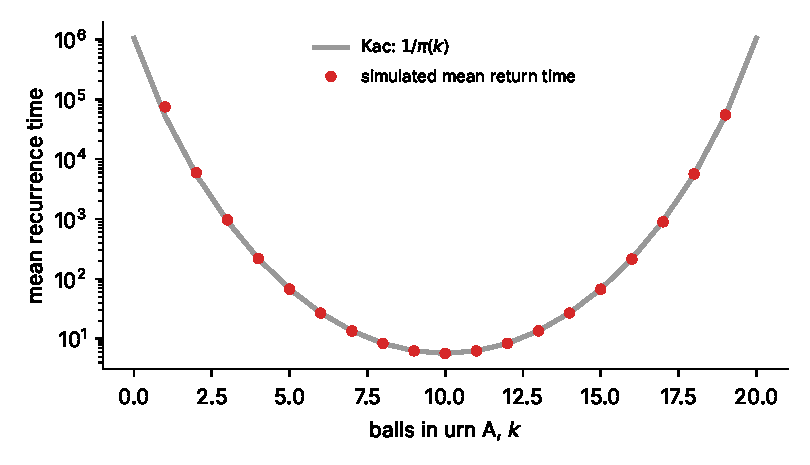
\includegraphics[width=0.85\textwidth]{figures/ehrenfest_kac.pdf}
\caption[Kac's lemma for the Ehrenfest urn]{Mean recurrence time to each state of the Ehrenfest urn with twenty balls, simulated over two million steps, against Kac's formula $1/\pi(k)$.}
\label{fig:ehrenfest}
\end{figure}

The same lemma governs topological freezing in lattice gauge theory. At weak coupling, configurations of nonzero topological charge occupy a small and shrinking fraction of the space accessible to local updates, and the time to tunnel between sectors is at least of the order of the inverse of the probability of the barrier configurations. Kac's lemma converts a statement about rare states into a statement about waiting times, and the split sampling and vertical likelihood methods of Section~\ref{ch:vertical} are, in this light, devices for reweighting the process so that rare states are no longer rare.

\subsection{The Feynman Kac formula}\label{sec:c5fk}

The most important of Kac's contributions for this book is the formula he found in 1949 after hearing Feynman describe path integrals. For a Schr\"odinger operator $H=-\frac12\Delta+V$,
\[
\big(e^{-tH}f\big)(x)=\E_x\Big[\exp\Big(-\int_0^tV(B_s)\,\mathrm ds\Big)f(B_t)\Big],
\]
where $B$ is Brownian motion started at $x$. The semigroup of the Hamiltonian is an expectation over Brownian paths weighted by the Euclidean action. Everything in Chapters~\ref{ch:positivity} and~\ref{ch:routeA} is an infinite dimensional version of this identity: the Euclidean measure on gauge fields is the path measure, the transfer matrix is $e^{-aH}$, and the correlation $C(\tau)=\langle O,e^{-\tau H}O\rangle$ is a Feynman Kac expectation. Reflection positivity is what makes the path measure define a positive semigroup.

The formula also suggests why the mass gap is a large deviation question. The spectral gap of $H$ is the exponential rate at which the Feynman Kac expectation forgets its initial condition. For a single particle in a confining potential this rate is controlled by how rarely Brownian paths wander into regions of high potential, and the Donsker Varadhan theory~\cite{DV75} of large deviations for occupation measures gives a variational formula for the bottom of the spectrum of $H$, though not for the gap above it. In gauge theory the analogue is the rate at which the Euclidean measure decorrelates across time slices.

\subsection{Can one hear the gap?}

Kac's 1966 paper \emph{Can one hear the shape of a drum?}~\cite{Ka66} asked whether the spectrum of the Laplacian determines the domain. His method was the heat trace: $\sum_ne^{-t\lambda_n}$ has a small time expansion whose coefficients are the area and perimeter of the drum and, as Kac conjectured and McKean and Singer~\cite{MS67} proved, its Euler characteristic. The partition functions of two dimensional Yang Mills in Chapter~\ref{ch:twod} are heat traces on the group, and the identity of Section~\ref{ch:riemann} that builds Riemann's kernel from the sphere partition function is a statement about the heat kernel of the three sphere. The mass gap asks for the lowest note of an infinite dimensional drum, and Kac's habit of reading geometry from heat traces is the habit this book has tried to apply.

Kac also left a short commentary~\cite{Ka74}, in P\'olya's collected papers, on how a lemma of P\'olya's about the Riemann $\xi$ function led to the Lee and Yang circle theorem. Chapter~\ref{ch:kacyang} opens with it.

\section{Jerrum, Sinclair and Randomised Polynomial Time}\label{ch:jerrum}\index{Jerrum, M.!and Sinclair, A.}\index{FPRAS}\index{canonical paths}

Is computing a lattice gauge partition function easy or hard? Complexity theory gives a precise answer for the Ising model, and the answer turns on the same structure that drives this book: positivity. This section explains the Jerrum and Sinclair algorithm, what it would mean to have an analogue for gauge theories, and how, for spin systems, rapid mixing of Markov chains is related to decay of correlations, which is not the mass gap.

\subsection{Approximate counting}\label{sec:c5counting}

A fully polynomial randomised approximation scheme (FPRAS) for a quantity $Z$ is a randomised algorithm that, given $\varepsilon$ and $\delta$, returns $\hat Z$ with $(1-\varepsilon)Z\le\hat Z\le(1+\varepsilon)Z$ with probability at least $1-\delta$, in time polynomial in the size of the input, $1/\varepsilon$ and $\log(1/\delta)$. Exact computation of partition functions is typically $\#$P hard. Approximate computation can be easy or hard depending on the model, and the boundary is where much of the interest lies.

\begin{theorem}[Jerrum and Sinclair~\cite{JS93}, 1993]
There is an FPRAS for the partition function of the ferromagnetic Ising model on an arbitrary graph, at any temperature, with a uniform external field.
\end{theorem}

The contrast with the antiferromagnet is a later result, not part of the theorem above: for parameters in the non uniqueness regime of the infinite $r$ regular tree, on the class of graphs of maximum degree $r$, approximate counting for the antiferromagnetic Ising model is NP hard, so no FPRAS exists for that class unless RP equals NP; on a bipartite graph such as $\Z^d$ the zero field antiferromagnet is equivalent to the ferromagnet and is easy (Sly and Sun~\cite{SS12}, and Galanis, \v{S}tefankovi\v{c} and Vigoda~\cite{GSV16}).

The algorithm has two ingredients. The first is a change of representation. The high temperature expansion writes the ferromagnetic Ising partition function as a sum over subgraphs with nonnegative weights, the ``subgraphs world'', and Jerrum and Sinclair built a Markov chain on subgraphs whose stationary law has these weights. The second is a proof of rapid mixing by canonical paths: every pair of states is joined by a path through the chain, and if no transition carries too many paths, the spectral gap of the chain is at most polynomially small. With a rapidly mixing sampler in hand, the partition function follows from a product of ratios along an annealing schedule,
\[
\frac{Z(\beta_K)}{Z(\beta_0)}=\prod_{i=0}^{K-1}\E_{\beta_i}\big[e^{-(\beta_{i+1}-\beta_i)H}\big],
\]
each estimated to small relative error with polynomially many samples. This product estimator is the discrete form of thermodynamic integration and of the power posterior ladder of Section~\ref{ch:vertical}.

\begin{figure}[t]
\centering
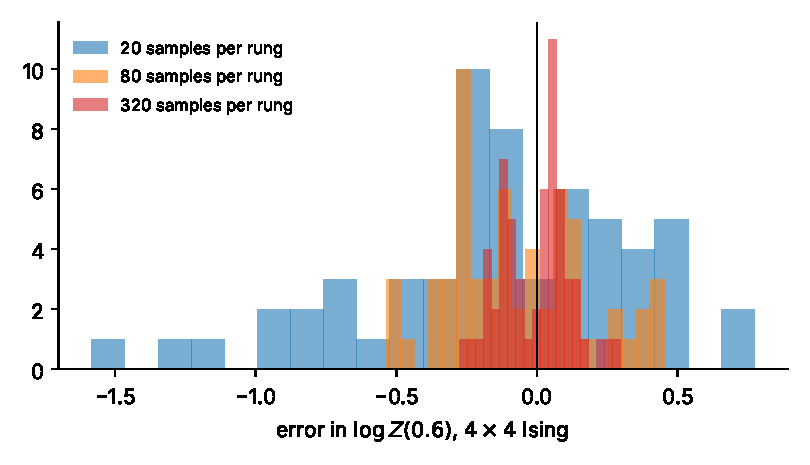
\includegraphics[width=0.85\textwidth]{figures/product_estimator.pdf}
\caption[A product estimator for the $4\times4$ Ising model]{Errors of a twelve rung product estimator for $\log Z(0.6)$ on the $4\times4$ Ising torus, against exact enumeration of all $65{,}536$ states, using Swendsen Wang moves at each rung, sixty repetitions for each sample size. The root mean square error falls from $0.50$ to $0.25$ to $0.12$ as the samples per rung grow from $20$ to $80$ to $320$.}
\label{fig:product}
\end{figure}

\subsection{Why positivity decides complexity}\label{sec:c5positivity}

The ferromagnetic case is easy. In the ferromagnet the high temperature expansion has nonnegative weights, so it defines a probability distribution that a Markov chain can sample. In the antiferromagnet some weights are negative, which is why standard arguments do not apply, but negativity alone does not decide the complexity: hardness holds only in the non uniqueness regime of the tree, as stated above, while in the uniqueness regime and on bipartite graphs in zero field the antiferromagnet is easy (Sly and Sun~\cite{SS12}, Galanis, \v{S}tefankovi\v{c} and Vigoda~\cite{GSV16}). The sign problem of quantum Monte Carlo is a related obstruction, not the same one.

Lattice gauge theory with nonnegative character coefficients, such as the Wilson action, is on the ferromagnetic side as far as the label factors go. The character expansion of Section~\ref{ch:latent} is its high temperature expansion, a sum over decorated surfaces whose weights $c_n$ are nonnegative, which by the Osterwalder Seiler theorem~\cite{OSe} is a sufficient condition for reflection positivity. A ``surfaces world'' Markov chain, the gauge analogue of the subgraphs world, would need the weight of each surface, after the links are integrated out, to be nonnegative; the characters change sign, and Section~\ref{ch:latent} does not claim this. Whether such a chain exists, and whether it mixes rapidly at weak coupling, is not known. The surfaces at weak coupling are large and fluctuating, and canonical path arguments that work for subgraphs have no evident analogue for closed surfaces with representation labels.

\begin{problem}\label{op:mixing1}
Is there an FPRAS for the partition function of SU(2) lattice gauge theory with the Wilson action, on boxes of side $L$, at every coupling, with running time polynomial in $L$?
\end{problem}

\subsection{Rapid mixing and the mass gap}

The question is not only algorithmic. For spin systems, a theorem of Martinelli and Olivieri~\cite{MO94}, building on Dobrushin and Shlosman~\cite{DS85,DS87} and on Stroock and Zegarlinski~\cite{SZ92}, says that for finite range interactions with a finite single spin space on $\Z^d$ the following are equivalent: the Glauber dynamics has a spectral gap, or a logarithmic Sobolev constant, bounded uniformly in the volume and in the boundary conditions; and the Gibbs measure has strong spatial mixing, exponential decay of correlations uniform in the boundary conditions. What the theorem relates is the spectral gap of a Markov chain at a fixed lattice coupling and the rate of decay of correlations of the lattice measure. It does not cover compact continuous spins or gauge fields, and the spectral gap of the chain is not the mass gap of the Hamiltonian, which is the spectral gap of the transfer matrix; nor does it say anything about the continuum limit. Strong spatial mixing uniform in the boundary conditions is also stronger than exponential decay of correlations in one phase: in the low temperature Ising model correlations decay exponentially in each pure phase, while the Glauber gap with free or periodic boundary conditions closes like $e^{-cL^{d-1}}$ on a box of side $L$ (sharp for $d=2$). Section~\ref{ch:dynamic} develops the relation, and Shen, Zhu and Zhu~\cite{SZZ} proved a mass gap for lattice Yang Mills at strong coupling by a stochastic analysis route of a related kind.

So rapid mixing of local Markov chains, the property that Jerrum and Sinclair needed, is connected, for spin systems under the hypotheses above, to exponential decay of correlations at a fixed lattice coupling, a lattice analogue of the property that the Clay problem asks for and not that property. At a critical point, local dynamics slow down polynomially, critical slowing down, and correlations decay polynomially. In a single phase with exponential decay of correlations and no dependence on the boundary, local dynamics mix exponentially fast; at phase coexistence they do not. For Yang Mills the continuum limit is reached as $\beta\to\infty$, where the correlation length in lattice units diverges and local dynamics must slow down. The right question is therefore not whether local dynamics mix rapidly uniformly in $\beta$, which they do not, but whether the relaxation time grows only as a fixed power of the correlation length, $\tau_{\mathrm{rel}}\sim\xi^z$ with $z$ independent of $\beta$ (compare the dynamic exponent in the next section): a statement about the renormalized dynamics along the ladder.

\subsection{Sampling log concave laws}

Our own early work on the complexity of sampling, with Frieze and Kannan~\cite{FKP}, building on Applegate and Kannan~\cite{AK91}, showed that log concave distributions on convex bodies can be sampled in random polynomial time. That result is the continuous analogue of the Jerrum and Sinclair theorem: log concavity plays the role of ferromagnetism, guaranteeing that local moves do not get trapped. Lattice gauge measures are not log concave (on the compact group a geodesically log concave function is constant, Chapter~\ref{ch:path}), and the Bakry \'Emery substitute, a positive lower bound on the Ricci curvature plus the Hessian of $\beta S$, fails at weak coupling because that Hessian is large and indefinite on the scale of the group, which is why the Bakry \'Emery curvature arguments~\cite{BE} of Section~\ref{ch:dynamic} and the stochastic quantization methods of Shen, Zhu and Zhu work only at strong coupling. In the vertical likelihood and P\'olya Gamma constructions, the role of latent variables is to restore log concavity conditionally, and the open question is whether a latent representation of gauge theory can do the same.

\subsection{What the complexity theory gives}

The complexity theory gives three things. The product estimator is the right way to compute partition functions along a renormalization ladder, and its error analysis is directly applicable. The ferromagnetic case, where positivity of the weights holds, is where positivity of the weights gives a Markov chain that can be analysed, which is one reason positivity matters computationally as well as physically. And for spin systems the equivalence between rapid mixing and spatial mixing relates decay of correlations at a fixed lattice coupling to the mixing of Markov chains, a relation whose extension to gauge fields is open and which Chapter~\ref{ch:path} weighs against the other routes.

\section{Sokal: Autocorrelation, Clusters and Zeros}\label{ch:sokal}\index{Sokal, A. D.}\index{autocorrelation time}\index{Edwards, R. G.!and Sokal, A. D.}\index{topological freezing}\index{Lee Yang zeros}

Alan Sokal's work touches almost every computational and structural question in this book. This section collects the parts that matter for the mass gap: the statistics of Markov chain Monte Carlo, cluster representations, multigrid methods, the zeros of partition functions, random walk representations, and the limits of perturbation theory.

\subsection{The statistics of Monte Carlo}\label{sec:c5stats}

Sokal's lecture notes on Monte Carlo methods in statistical mechanics set the standard for how simulation output should be analysed. The central quantity is the integrated autocorrelation time
\[
\tau_{\mathrm{int}}=\tfrac12+\sum_{\ell\ge1}\rho(\ell),
\]
which inflates the variance of a sample mean by a factor $2\tau_{\mathrm{int}}$. Estimating it requires truncating the sum of empirical autocorrelations, because the noise in the partial sum of the empirical autocorrelations grows with the lag. Madras and Sokal's~\cite{MS88} automatic windowing truncates at the first lag $W$ with $W\ge c\,\hat\tau_{\mathrm{int}}(W)$, with $c$ around five or six, balancing bias against variance. Every autocorrelation time in this chapter was estimated that way, with the caveat that where the window cannot close within the run, as at $\beta=6$ below, the estimate is a lower bound.

Sokal also emphasised dynamic critical exponents: near a critical point the autocorrelation time of a local algorithm grows like $\xi^z$ with $z\approx2$, the critical slowing down that made cluster algorithms necessary.

\subsection{Clusters: Edwards and Sokal}\label{sec:c5clusters}

Edwards and Sokal~\cite{ES88} identified the joint distribution of spins and bonds behind the Swendsen and Wang algorithm~\cite{SW87}, and generalised it beyond Potts models. The joint law couples the spin model to the Fortuin Kasteleyn random cluster model~\cite{FK72}, and its conditionals are the two steps of the algorithm: given spins, open bonds between agreeing neighbours independently; given bonds, colour clusters independently. Figure~\ref{fig:sw} shows the payoff on a $24\times24$ Ising torus: near the critical coupling the autocorrelation time of the absolute magnetisation $|M|$ is about twenty sweeps for Metropolis and about four steps for Swendsen and Wang.

\begin{figure}[t]
\centering
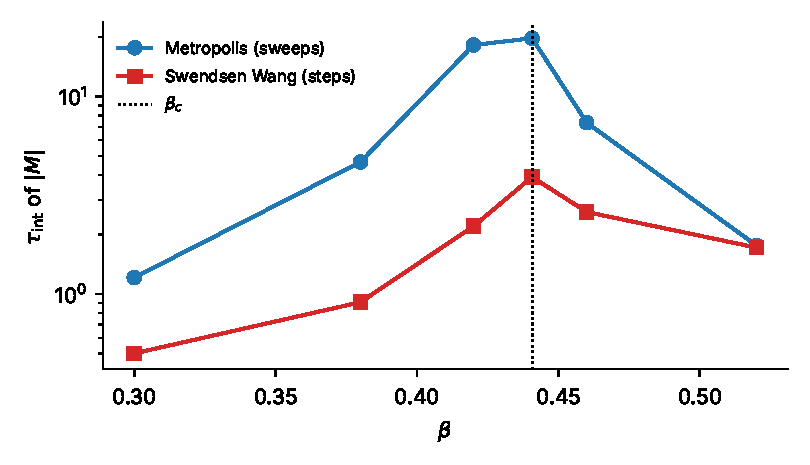
\includegraphics[width=0.85\textwidth]{figures/sw_vs_metropolis.pdf}
\caption[Swendsen Wang against Metropolis near criticality]{Integrated autocorrelation time of $|M|$ on a $24\times24$ Ising torus, estimated by Madras and Sokal windowing, for checkerboard Metropolis and for Swendsen and Wang. The peak at $\beta_c$ is critical slowing down; the cluster algorithm largely removes it.}
\label{fig:sw}
\end{figure}

For this book the Edwards and Sokal construction matters for a second reason. Its joint law is a coupling, and couplings are how monotonicity and decay of correlations are proved for the random cluster model. Chapter~\ref{ch:path} asks for a coupling between a true block spin step and a Migdal Kadanoff step, and the Edwards and Sokal construction is the template.

\subsection{Multigrid Monte Carlo}

Goodman and Sokal~\cite{GS89} introduced multigrid Monte Carlo, which updates the field at a hierarchy of scales by moving coarse grained variables, in direct analogy with multigrid methods for elliptic equations. For Gaussian models it eliminates critical slowing down. For nonlinear models the gain depends on how well the coarse moves respect the effective action at each scale, which is the same question the renormalization group asks. A multigrid sampler for gauge theory whose coarse levels follow the Migdal Kadanoff ladder would be a computational test of the ladder itself.

\subsection{Topological freezing}

The analogue of critical slowing down in lattice gauge theory is topological freezing. In two dimensional U(1) lattice gauge theory the topological charge $Q$, the total winding of the plaquette angles, is an integer, and changing it requires passing through configurations of high action. Figure~\ref{fig:u1} shows Metropolis histories of $Q$ on a $20\times20$ torus: at $\beta=1$ the charge decorrelates in about one sweep, at $\beta=3$ in about thirty six, at $\beta=6$ in more than four hundred, and at $\beta=10$ it did not change once in three thousand sweeps. In four dimensional SU(3) the same phenomenon limits how close to the continuum glueball masses can be measured. Kac's lemma (Section~\ref{sec:c5kaclemma}) gives a lower bound for the growth, and split sampling across sectors from Section~\ref{ch:vertical} is one remedy.

\begin{figure}[t]
\centering
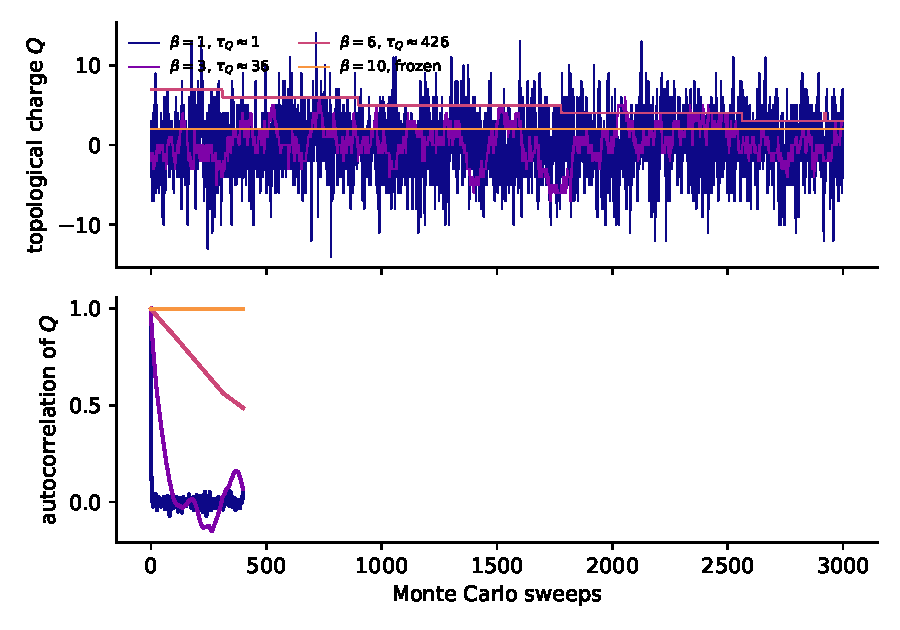
\includegraphics[width=\textwidth]{figures/u1_topology.pdf}
\caption[Topological freezing in two dimensional U(1) lattice gauge theory]{Topological charge histories and autocorrelations for two dimensional U(1) lattice gauge theory on a $20\times20$ torus with Metropolis updates. The integrated autocorrelation time grows from about one sweep at $\beta=1$ to over four hundred at $\beta=6$; at $\beta=10$ the charge is frozen.}
\label{fig:u1}
\end{figure}

\subsection{Zeros of partition functions}\label{sec:c5zeros}

Lee and Yang~\cite{LY52} proved in 1952 that the zeros of the ferromagnetic Ising partition function in the complex fugacity $e^{-2\eta}$ lie on the unit circle. Fisher studied the zeros in the complex temperature, which pinch the real axis at a critical point. Sokal~\cite{So01} extended zero free region results to Potts models and chromatic polynomials, proving that the zeros of the chromatic polynomial of a graph of maximum degree $r$ lie in a disc of radius proportional to $r$, and with Scott~\cite{SS05} connected zero free regions of the hard core gas to the Lov\'asz local lemma.

\begin{figure}[t]
\centering
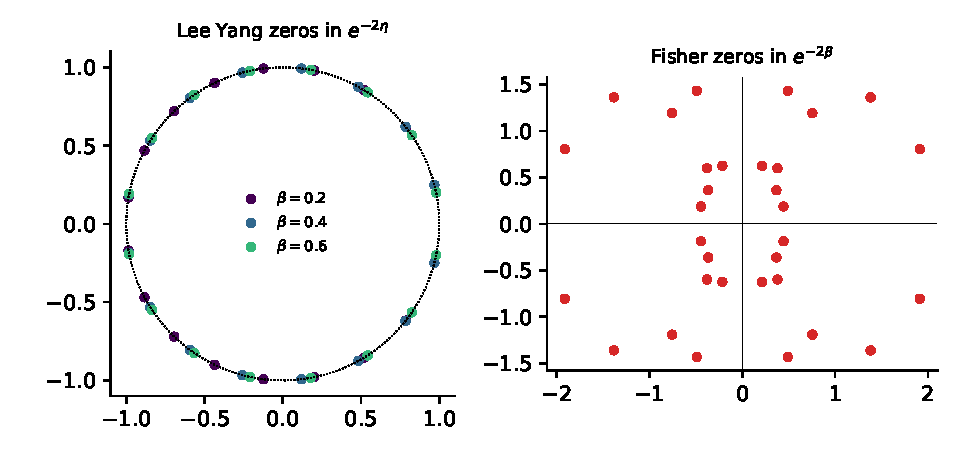
\includegraphics[width=\textwidth]{figures/lee_yang_fisher.pdf}
\caption[Lee Yang and Fisher zeros of the $4\times4$ Ising model]{Left: zeros of the $4\times4$ Ising partition function in $e^{-2\eta}$ at three couplings, all on the unit circle as the Lee Yang theorem requires. Right: zeros in the complex temperature variable $e^{-2\beta}$.}
\label{fig:leeyang}
\end{figure}

Zeros connect three threads of this book. The Lee Yang property is the ferromagnetic random variable condition behind Newman's approach~\cite{Ne76} to the Riemann Hypothesis, which our Riemann programme uses. Zero free regions of a partition function in a complex coupling imply analyticity of the free energy, and analyticity in the coupling across the whole range $0<\beta<\infty$ is exactly the absence of a phase transition that the crossover argument of Chapter~\ref{ch:path} needs. And whether the Fisher zeros of the two dimensional sphere theory can be related, through the identity of Section~\ref{ch:riemann}, to the zeros of $\Xi$ is posed there as an open problem.

\subsection{Random walks, triviality and Borel summability}

Brydges, Fr\"ohlich and Spencer~\cite{BFS82} gave a random walk representation of correlation functions in $\phi^4$ theory, Aizenman and Fr\"ohlich~\cite{Ai82,Fr82} used such representations to prove triviality above four dimensions, and Fern\'andez, Fr\"ohlich and Sokal~\cite{FFS92} gave the systematic account; Aizenman and Duminil Copin~\cite{ADC21} later proved marginal triviality in four. The contrast is instructive: $\phi^4_4$ is marginal and trivial, its coupling running to zero at long distances, while Yang Mills is marginal and asymptotically free, its coupling running to zero at short distances. The two differ by the sign of the one loop term in the beta function. In Section~\ref{ch:mk} that sign is the sign of the curvature of the group, carried by $\E S_{\mathrm{BPY}}>0$.

Sokal's 1980 improvement of Watson's theorem~\cite{So80} gives sharp conditions under which a function is the Borel sum of its asymptotic series. Perturbation theory in Yang Mills is expected to fail those conditions: the series is expected to have renormalon singularities on the positive Borel axis, and a mass gap, if it exists, is a renormalization group invariant mass and so of order $\Lambda=\mu e^{-1/(2b_0g^2)}$, invisible to every order. That is a precise sense in which the gap is nonperturbative, and why the renormalization group must be followed into strong coupling.

\subsection{What Sokal's methods give}

Madras and Sokal windowing is the correct way to quote errors on every Monte Carlo number in this book. Edwards and Sokal is the model for the coupling the comparison step needs. Multigrid is the natural computational test of the ladder. Zero free regions are the analytic form of the no phase transition hypothesis. And the contrast with $\phi^4_4$ isolates the sign that makes Yang Mills different.

\section{Slice Variables, Log Concavity and Besag}\label{ch:slice}\index{slice sampling}\index{Besag, J.}\index{pseudolikelihood}\index{Markov random field}\index{log concavity}\index{Higdon, D.}

Section~\ref{ch:latent} used latent variables as samplers. This section isolates the trick that makes them work, the use of slice variables to turn a hard conditional into a log concave one, in the form given by Polson~\cite{Po96} in 1996 and by Higdon~\cite{Hi98} in 1998. It then applies the trick to the SU(2) link conditional, where positive curvature would turn it into a mixing bound (conditionally on a claim whose proof is only sketched), and asks whether Besag's theory of Markov random fields is useful for the mass gap.

\subsection{The slice variable trick}\label{sec:c5slice}

Let the target be $\pi(x)\propto p(x)\prod_{i=1}^mL_i(x)$ on $\R^d$. Introduce one uniform slice variable $w_i$ for each factor, written $w=(w_1,\dots,w_m)$,
\[
\pi(x,w)\propto p(x)\prod_{i=1}^m\mathrm{I}\{0<w_i<L_i(x)\}.
\]
The $x$ marginal is $\pi$. Given $x$, the $w_i$ are independent uniforms. Given $w$, $x$ has density proportional to $p$ restricted to the set $C(w)=\bigcap_i\{x:L_i(x)>w_i\}$.

\begin{proposition}\label{prop:slicelc}
If $p$ is log concave and every $L_i$ is quasi concave, meaning that its superlevel sets are convex, then for every $w$ the conditional law of $x$ given $w$ is log concave.
\end{proposition}

\begin{proof}
$C(w)$ is an intersection of convex sets, hence convex, and the indicator of a convex set is log concave. A product of log concave functions is log concave.
\end{proof}

The point is that quasi concavity is much weaker than log concavity. A Cauchy likelihood $L(x)=(1+(y-x)^2)^{-1}$ is not log concave, and a posterior built from several of them can be multimodal, but each factor is unimodal, so its superlevel sets are intervals. After slicing, every conditional is a log concave density on a convex set. Frieze, Kannan and Polson~\cite{FKP} showed that such densities can be sampled in time polynomial in the dimension, by a random walk whose conductance is controlled by the isoperimetry of log concave measures. The slice variables thus move the difficulty out of the $x$ conditional and into the slice variables, which are one dimensional, and into the geometry of the sets $C(w)$. This does not make the joint chain rapidly mixing: for a multimodal target the slice levels must still pass through the gaps between modes, and the chain can mix slowly.

Polson's 1996 analysis~\cite{Po96} of the convergence of Markov chain Monte Carlo used the scale mixture version of the same device. Since
\[
\frac{1}{1+z^2}=\int_0^\infty e^{-\lambda(1+z^2)}\,\mathrm d\lambda,
\]
a Cauchy likelihood is a mixture of Gaussian likelihoods over a latent precision. Given the precisions the posterior is Gaussian, hence log concave, but log concavity of one block does not by itself bound the rate of the chain that alternates precisions and location, which is governed by the dependence between the two blocks. This is the same structure as the P\'olya Gamma augmentation of Polson, Scott and Windle~\cite{PSW13} for logistic models, and the same structure as the character expansion of lattice gauge theory, in which a positive latent label renders each conditional tractable (Section~\ref{ch:latent}).

\subsection{Higdon: auxiliary variables and partial decoupling}\label{sec:c5higdon}

Higdon's 1998 paper~\cite{Hi98} organised these ideas for spatial models. For a Potts model with weight $\prod_{\langle ij\rangle}e^{\beta\,\mathrm I\{x_i=x_j\}}$, slicing each bond factor with $w_{ij}\sim\mathrm{Uniform}(0,e^{\beta\mathrm I\{x_i=x_j\}})$ yields the Swendsen and Wang algorithm: a bond whose slice exceeds one forces its endpoints to agree, and the conditional of the spins given the slices is uniform over colourings of the resulting clusters. Partial decoupling slices only a fraction $\delta$ of each factor, $e^{\delta\beta\mathrm I}$, and keeps $e^{(1-\delta)\beta\mathrm I}$ in the conditional, so that clusters are smaller and the remaining interaction keeps the image model faithful. The parameter $\delta$ interpolates between a local heat bath at $\delta=0$ and full Swendsen and Wang at $\delta=1$.

\subsection{Slicing the SU(2) link}

For a link $U$ of two dimensional or four dimensional SU(2) lattice gauge theory, the conditional given its neighbours is
\[
\pi(U\mid\cdot)\propto\exp\Big(\beta\sum_{p\ni U}\tfrac12\operatorname{tr}(UV_p)\Big)\,\mathrm dU,
\]
a product over the plaquettes containing the link, with $V_p$ the staple of plaquette $p$. Identify SU(2) with the unit sphere $S^3$. Each factor is a monotone function of the geodesic distance from $U$ to $V_p^{-1}$, so its superlevel sets are geodesic balls, spherical caps. Slice each plaquette factor separately. Given the slices, $U$ is Haar distributed on the intersection of caps
\[
C(w)=\bigcap_{p\ni U}\big\{U:\tfrac12\operatorname{tr}(UV_p)>c_p\big\}.
\]
The level $c_p$ is related to the slice variable $w_p\in(0,e^{\beta a_p})$ of plaquette $p$, where $a_p=\frac12\operatorname{tr}(UV_p)$, by $c_p=\log w_p/\beta$.

\begin{conjecture}\label{prop:slicecurv}
If every slice level satisfies $c_p>0$, then $C(w)$ is geodesically convex, and the uniform law on $C(w)$, with the reflected Brownian motion on it, satisfies a logarithmic Sobolev inequality with constant $2$, independent of $\beta$ and of the staples.
\end{conjecture}

\begin{proof}[Evidence: sketch of a proof, not a complete proof]
\renewcommand{\qedsymbol}{}
A spherical cap smaller than a hemisphere is geodesically convex in $S^3$, and intersections of geodesically convex sets are geodesically convex. The unit three sphere has Ricci curvature $2$. On a smooth geodesically convex domain of a manifold with $\mathrm{Ric}\ge\kappa>0$, the uniform law with reflecting boundary satisfies the Bakry \'Emery criterion~\cite{BE} with constant $\kappa$, because convexity makes the boundary term in the Bochner formula nonnegative. This is the Bakry \'Emery theorem with a Neumann boundary, for which we have no reference in the bibliography. The set $C(w)$ is an intersection of caps and has corners, so the last step needs an approximation by smooth convex domains, which we do not carry out.
\end{proof}

Figure~\ref{fig:caps} shows the picture one dimension down, on $S^2$: four caps smaller than hemispheres, and their intersection, which is convex.

\begin{figure}[t]
\centering
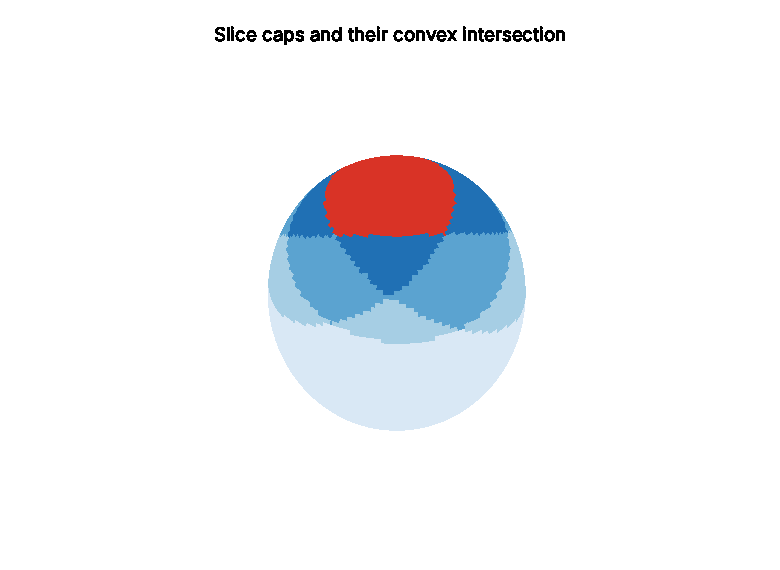
\includegraphics[width=0.7\textwidth]{figures/slice_caps.pdf}
\caption[Slice caps on the sphere]{Four spherical caps on $S^2$, shaded by how many contain each point, and their intersection in red. Each cap is smaller than a hemisphere, so the intersection is geodesically convex.}
\label{fig:caps}
\end{figure}

The claim, if it holds, is the Riemannian version of Proposition~\ref{prop:slicelc}, with the curvature of the group doing the work that log concavity of the prior does in flat space. It would say that, given the slices, the group causes no difficulty, since the bound is uniform in $\beta$ and in the staples; whatever slows the joint chain lives in the slice levels, which are one dimensional per plaquette. By analogy with the curvature of the group that drives asymptotic freedom in Section~\ref{ch:mk}, the curvature of $S^3$ would be the constant in the log Sobolev inequality of the sliced conditional (we do not claim that the two are the same quantity). This would be a small step toward the dynamic sandwich of Section~\ref{ch:isthere}, where one needs uniform log Sobolev constants along the ladder.

The single link heat bath of Section~\ref{ch:latent} is the special case in which the staples of the plaquettes are summed before slicing. The condition $c_p>0$ fails only for slices with $w_p\le1$, the value of the plaquette factor at the Haar median $a_p=0$, and these become rare as $\beta$ grows.

\subsection{Besag and Markov random fields}\label{sec:c5besag}

Besag's 1974 paper~\cite{Be74} gave the statistical theory of spatial interaction on lattices: the Hammersley and Clifford theorem, which says that a positive distribution with the local Markov property is a Gibbs distribution with interactions on cliques; the coding method, which partitions the lattice into conditionally independent sets; and, in 1975~\cite{Be75}, the pseudolikelihood, the product of all local conditionals, as an estimator for parameters whose likelihood involves an intractable partition function. Later work gave iterated conditional modes for image restoration, the intrinsic conditional autoregression of Besag, York and Molli\'e~\cite{BYM} for disease mapping, and with Green~\cite{BG93} the synthesis of spatial statistics and Markov chain Monte Carlo.

Each of these is useful here.
\begin{enumerate}
\item A lattice gauge field is a Markov random field on links with plaquette cliques, and the Wilson measure is the Gibbs distribution of Hammersley and Clifford. Reflection positivity is a stronger, global property, but the local Markov property is what makes heat bath, coding and multilevel algorithms work. The checkerboard update of Section~\ref{ch:sokal} is Besag's coding method.
\item The intrinsic conditional autoregression on a lattice is the massless lattice free field. Its precision matrix, the graph Laplacian, has an exact zero mode, the constant field, so the model is improper; but that impropriety is not the absence of a mass gap. The absence of a gap is that the lowest nonzero eigenvalue of the Laplacian on mean zero fields tends to zero as the lattice grows ($4\sin^2(\pi/L)$ on a periodic $L\times L$ torus along one axis), and the usual sum to zero constraint, which removes the impropriety, leaves the model gapless. Adding a mass term $m$ makes it proper and gives a finite correlation length, approximately $1/m$ for small $m$. Statisticians have long used, in the ICAR, a model that is gapless in the large lattice limit.
\item Pseudolikelihood estimates couplings from configurations without computing a partition function. Its score equation is a Schwinger Dyson identity, and in lattice gauge theory the same idea appears as inverse Monte Carlo and as the matching step of Swendsen's Monte Carlo renormalization group~\cite{Sw79}. It is the tool the open problem of Chapter~\ref{ch:path} needs: block a lattice configuration, fit the plaquette law of the blocked field by pseudolikelihood, and compare the fitted law with the Migdal Kadanoff prediction rung by rung.
\end{enumerate}

\subsection{Pseudolikelihood for SU(2)}\label{sec:c5pl}

For SU(2) the pseudolikelihood is explicit. Write the summed staple of a link as $kV$ with $V\in$ SU(2) and $k\ge0$, and let $a_0=\frac12\operatorname{tr}(UV)$. The conditional density of $a_0$ is proportional to $\sqrt{1-a_0^2}\,e^{\beta ka_0}$, with mean $I_2(\beta k)/I_1(\beta k)$. The maximum pseudolikelihood estimate of $\beta$ therefore solves
\[
\sum_{\text{links}}k\Big(a_0-\frac{I_2(\beta k)}{I_1(\beta k)}\Big)=0,
\]
a one dimensional monotone equation. We generated configurations of two dimensional SU(2) on a $12\times12$ torus by the slice heat bath at four couplings, and solved the equation on eight configurations at each coupling. The standard error in the table is the standard deviation over the eight configurations divided by $\sqrt8$; the configurations are consecutive in one chain, ten sweeps apart, so it is somewhat optimistic.

\begin{center}
\small
\begin{tabular}{ccc}
\toprule
true $\beta$ & mean estimate & standard error \\ \midrule
1 & 1.131 & 0.053 \\
2 & 2.122 & 0.096 \\
4 & 3.844 & 0.083 \\
8 & 8.436 & 0.114 \\
\bottomrule
\end{tabular}
\end{center}


\begin{figure}[t]
\centering
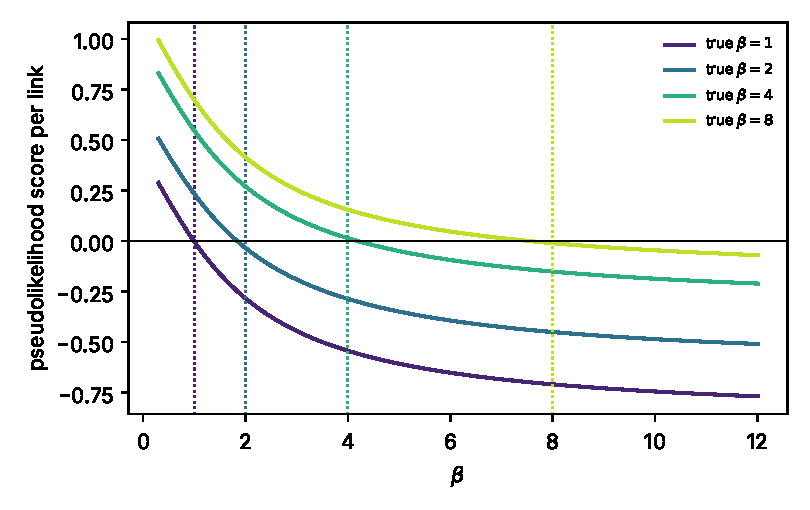
\includegraphics[width=0.85\textwidth]{figures/pl_score.pdf}
\caption[Pseudolikelihood scores for SU(2)]{Pseudolikelihood score per link as a function of $\beta$ for synthetic link conditionals at four true couplings. Each score is decreasing and crosses zero near the true value, marked dotted.}
\label{fig:plscore}
\end{figure}

Figure~\ref{fig:plscore} shows why the equation is easy to solve: the score is monotone and crosses zero steeply. A single configuration of $288$ links fixes the coupling to about fifteen percent at $\beta\le2$ and to about five percent at $\beta\ge4$, with no partition function. The means at $\beta=1$ and $\beta=8$ lie above the true value by about two and a half and four standard errors; we have not diagnosed whether this is a bias of the estimator or of the sampler. Pseudolikelihood is consistent for Gibbs fields under mild conditions, as Comets~\cite{Co92} proved, though not efficient at strong dependence. For the ladder the relevant estimate is not a single $\beta$ but the whole plaquette law, parametrised by its character coefficients $u_n$; the same equations, with the Wilson factor replaced by a character sum, give it.

\subsection{What slicing and Besag give}

Slicing and Besag give three things. The slice variable trick makes the conditionals of heat bath samplers for gauge fields tractable and locates the difficulty in the slice levels, though it does not by itself guarantee fast mixing of the joint chain. In its Riemannian form it would turn the curvature of the group into an explicit log Sobolev constant for the sliced conditional, if the claim above is confirmed, which is a building block for the dynamic route to the gap. And Besag's pseudolikelihood is the right estimator for the empirical renormalization ladder: it fits effective plaquette laws of blocked configurations cheaply, and consistently under mild conditions, which is what testing the Migdal Kadanoff caricature against the real theory requires.

\section*{Exercises}
\begin{enumerate}
\item Prove Kac's lemma for a finite irreducible Markov chain (Section~\ref{sec:c5kaclemma}).
\item Show that the expected number of returns of simple random walk by time $n$ grows like $\log n$ in two dimensions (Section~\ref{sec:c5polya}).
\item Derive the Feynman Kac formula for a bounded continuous potential from the Trotter product formula (Section~\ref{sec:c5fk}).
\item Derive the product estimator and bound its relative variance in terms of the variances of the ratios at each rung (Section~\ref{sec:c5counting}).
\item Write the high temperature expansion of the Ising model and show that its weights are nonnegative for ferromagnetic couplings (Section~\ref{sec:c5positivity}).
\item Write the character expansion of SU(2) lattice gauge theory as a sum over surfaces and identify the analogue of the subgraphs world (Section~\ref{sec:c5positivity}).
\item Show that the variance of a sample mean of a stationary chain is approximately $2\tau_{\mathrm{int}}\sigma^2/n$ (Section~\ref{sec:c5stats}).
\item Derive the Swendsen and Wang conditionals from the Edwards and Sokal joint law, and again by slicing the bond factors as in Higdon's auxiliary variables (Sections~\ref{sec:c5clusters} and~\ref{sec:c5higdon}).
\item Verify the Lee Yang theorem for the Ising model on two sites (Section~\ref{sec:c5zeros}).
\item Show that the slice sampler for a single Cauchy likelihood with a Gaussian prior samples a truncated Gaussian given the slice (Section~\ref{sec:c5slice}).
\item Show that the score of the SU(2) pseudolikelihood has negative derivative in $\beta$ whenever some $k>0$, so that the estimate is unique (Section~\ref{sec:c5pl}).
\item Show that the ICAR precision matrix on a torus has a one dimensional null space (Section~\ref{sec:c5besag}).
\end{enumerate}

\chapter{Hitting Times and Learning the Gap}\label{ch:hitting}\index{hitting time}\index{moderate deviations}\index{hazard rate}

A gap is a rate, and probability has more than one way to read a rate. The correlator reads it from the decay of a covariance, and Chapter~\ref{ch:kac} read it from the mixing of a Markov chain. This chapter records two further readings: the hazard rate of a hitting time, in the manner of Roberts and Shortland \cite{RS95,RS97}, and the scale of fluctuations between the central limit theorem and large deviations, in the manner of Rubin and Sethuraman \cite{RuSe65}. The hazard rate gives a theorem about the gap and an estimator. The moderate deviation scale gives honest sample sizes and, under a hypothesis we state, a necessary test for a unique vacuum. Neither proves the gap in four dimensions. We say where each helps.

The second part of the chapter turns from what the gap is to how it is learned. Section~\ref{ch:plgbc} develops sufficient statistics of a lattice gauge field, particle learning \cite{CJLP} and generative Bayesian computation \cite{PSgbc}, which learns the map from statistics to parameters from simulations, and asks whether they are useful for the mass gap. Section~\ref{ch:quantum} asks what quantum computation could add \cite{PSX23}. The chapter closes Part II: apart from the theorems proved for one group variable and one plaquette, everything in it is an estimator, a restatement or a numerical experiment.

\section{The hazard rate of a hitting time}\index{Roberts, G. O.}\index{Shortland, C. F.}

Roberts and Shortland studied the first time a diffusion hits a boundary through its hazard rate $r(t)=-\frac{d}{dt}\log P(T>t)$, approximated it by tangent boundaries, and used the result to price barrier options with time dependent coefficients. The object that matters for us is the limit of the hazard rate. For a reversible diffusion with generator $L$ and invariant probability $\mu$, and a closed set $A$ with $\mu(A)>0$, let
\[
\lambda_D(A)=\inf\Big\{\frac{\mathcal E(f,f)}{\mu(f^2)}:\ f=0\ \text{on}\ A\Big\},\qquad \mathcal E(f,f)=\mu\big(f(-L)f\big),
\]
be the bottom of the spectrum with Dirichlet condition on $A$. When $\lambda_D(A)$ is an isolated eigenvalue, as on a compact state space, $P_\nu(T_A>t)$ decays like $e^{-\lambda_D(A)t}$ for every starting law $\nu$ with a square integrable density that charges the ground state, and the hazard rate of $T_A$ tends to $\lambda_D(A)$. The gap $\lambda_1$ is the bottom of the spectrum on functions of mean zero.

\begin{theorem}[Hitting times bracket the gap]\label{thm:hitgap}\index{Dirichlet eigenvalue}
For a reversible diffusion with invariant probability $\mu$ and gap $\lambda_1$:
\begin{enumerate}
\item[(i)] for every closed set $A$ with $\mu(A)>0$, $\lambda_1\le\lambda_D(A)/\mu(A)$;
\item[(ii)] $\lambda_1\ge\inf\{\lambda_D(A):\mu(A)\ge\frac12\}$.
\end{enumerate}
Hence, writing $r_*$ for the infimum in (ii), $r_*\le\lambda_1\le2r_*$: the gap is positive if and only if $\lambda_D(A)$ is bounded away from zero over the closed sets of measure at least one half; on a compact state space $\lambda_D(A)$ is the limiting hazard rate of $T_A$.
\end{theorem}

\begin{proof}
(i) If $f$ vanishes on $A$ then by the Schwarz inequality $\mu(f)^2\le\mu(f^2)\,\mu(A^c)$, so $\operatorname{Var}_\mu(f)\ge\mu(A)\,\mu(f^2)$, and the Poincar\'e inequality gives $\mathcal E(f,f)\ge\lambda_1\mu(A)\mu(f^2)$. (ii) Let $f$ be in the domain of the form, let $m$ be a median of $f$, and put $f_\pm=(f-m)_\pm$. Each of $f_+$ and $f_-$ vanishes on a set of measure at least one half, so $\mu(f_\pm^2)\le\mathcal E(f_\pm,f_\pm)/r_*$ by the definition of $r_*$. The form of a diffusion is local, $\mathcal E(f_+,f_-)=0$, so $\mathcal E(f_+,f_+)+\mathcal E(f_-,f_-)=\mathcal E(f,f)$. Hence $\operatorname{Var}_\mu(f)\le\mu\big((f-m)^2\big)=\mu(f_+^2)+\mu(f_-^2)\le\mathcal E(f,f)/r_*$, which is $\lambda_1\ge r_*$; no eigenfunction is needed, so it does not matter whether the gap is attained. The last statement takes $\mu(A)\ge\frac12$ in (i).
\end{proof}

Both halves are standard for Markov chains, beside Cheeger's inequality; we have not seen them used for the mass gap. The change of object is the point. A correlator is a signed quantity whose signal to noise ratio falls exponentially in time; a survival probability is positive, and the maximum likelihood estimate of a constant hazard is a ratio of sufficient statistics, the number of exits divided by the total time at risk.

When there is a reflection, the factor of two disappears.

\begin{proposition}[Reflection]\label{prop:hitreflect}\index{reflection positivity}
Let $\rho$ be an involution of the state space that preserves $\mu$ and commutes with $L$, and suppose that the complement of its fixed set $F$ has exactly two components, each connected and exchanged by $\rho$, so that every continuous path from a point to its image meets $F$. Then the lowest eigenvalue of $-L$ on functions odd under $\rho$ equals $\lambda_D(F)$. In particular $\lambda_1\le\lambda_D(F)$, with equality when the first excited state is odd.
\end{proposition}

\begin{proof}
An odd eigenfunction vanishes on $F$, so its restriction to one side is a Dirichlet eigenfunction; conversely the odd extension of the Dirichlet ground state on one side is an odd eigenfunction of $L$, and it is the lowest because the Dirichlet ground state has no zeros.
\end{proof}

\section{The example of SU(2)}

Take Brownian motion on $SU(2)=S^3$ with generator $\frac12\Delta_{S^3}=2\Delta$. Here $\Delta_{S^3}$ is the Laplacian of the unit sphere and $\Delta$ that of this book, so that the law at time $t$ is the heat kernel $K_{2t}$. Write $U=a_0+i\,a\cdot\sigma$. The class functions $\sin(n\theta)/\sin\theta$ with $a_0=\cos\theta$ are eigenfunctions with eigenvalues $\frac12(n^2-1)$, so the gap is $\frac32$, attained by $\chi_2=2a_0$. The map $U\mapsto-U^\dagger$ sends $a_0$ to $-a_0$ and fixes the equator $\{a_0=0\}$, and $\chi_2$ is odd. Let $T$ be the first time the motion started at the identity reaches the equator.

\begin{proposition}\label{prop:equator}
\[
P(T>t)=\frac{16}{\pi}\sum_{k\ge1}(-1)^{k+1}\frac{k^2}{4k^2-1}\,e^{-(4k^2-1)t/2},
\]
so the hazard rate of $T$ tends to $\frac32$, the spectral gap of this Brownian motion, with the next correction of relative size $e^{-6t}$.
\end{proposition}

\begin{proof}
The Dirichlet eigenfunctions on the hemisphere are $\phi_k=\sin(2k\theta)/\sin\theta$ with eigenvalues $\frac12(4k^2-1)$. With respect to $\sin^2\theta\,d\theta$ on $[0,\pi/2]$ they have squared norm $\pi/4$, value $2k$ at $\theta=0$, and integral $\int_0^{\pi/2}\sin(2k\theta)\sin\theta\,d\theta=(-1)^{k+1}2k/(4k^2-1)$. Expanding the point mass at the identity gives the series.
\end{proof}

\begin{figure}[t]
\centering
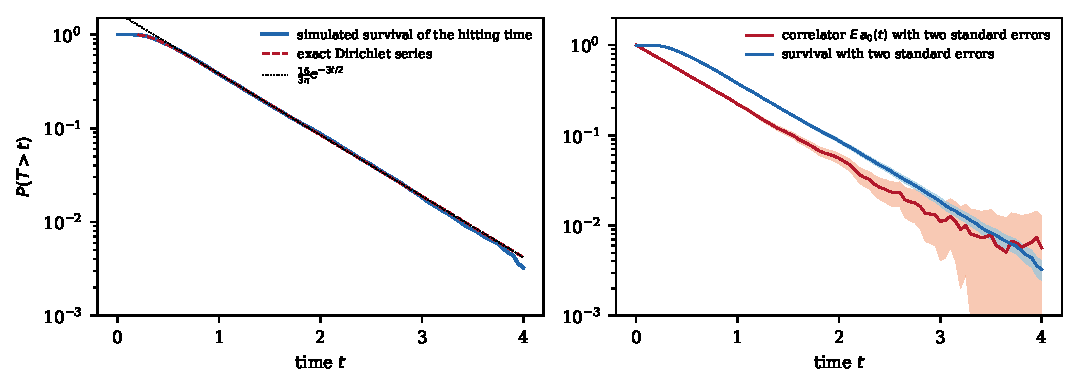
\includegraphics[width=0.85\textwidth]{figures/hitting_gap.pdf}
\caption[The gap of SU(2) from a hitting time]{Brownian motion on SU(2) started at the identity, twenty thousand paths. Left: the survival probability of the first hitting time of the equator, with the exact series of Proposition~\ref{prop:equator} and its leading term. Right: the survival probability and the correlator $\E a_0(t)=e^{-3t/2}$ from the same paths, each with a band of two standard errors. Both decay at the gap; the band of the survival probability stays narrow in relative terms for longer.}
\label{fig:hitgap}
\end{figure}

We simulated twenty thousand paths with step $0.002$, with a Brownian bridge correction for crossings between steps, without which the rate was biased down by about five percent in a single run. Both estimators use the same paths, and the errors of the effective mass are standard errors by the delta method with the empirical covariance of the two time points over those paths.

\begin{center}
\small
\begin{tabular}{lcc}
\toprule
estimator & window & estimate of the gap $\frac32$ \\ \midrule
hazard rate, exits over time at risk & $t>0.5$ & $1.452\pm0.012$ \\
hazard rate & $t>1$ & $1.497\pm0.017$ \\
hazard rate & $t>1.5$ & $1.491\pm0.025$ \\
effective mass of $\E a_0$ & $0$ to $0.5$ & $1.494\pm0.011$ \\
effective mass of $\E a_0$ & $0.5$ to $1$ & $1.520\pm0.027$ \\
effective mass of $\E a_0$ & $1$ to $1.5$ & $1.488\pm0.059$ \\
effective mass of $\E a_0$ & $1.5$ to $2$ & $1.27\pm0.11$ \\
effective mass of $\E a_0$ & $2$ to $2.5$ & $1.70\pm0.26$ \\
\bottomrule
\end{tabular}
\end{center}

At equal cost, for windows that start after $t=1$, the hitting time gives the gap three and a half times more precisely than the correlator, a factor of about twelve in sample size, and its error grows slowly as the window moves out where the correlator's grows exponentially (Figure~\ref{fig:hitgap}), because every surviving path contributes to the hazard estimate with a positive weight. The advantage does not extend to the correlator's earliest window: $0$ to $0.5$ is as good as the hazard rate ($\pm0.011$ against $\pm0.017$), because $a_0=\frac12\chi_2$ is an exact eigenfunction with no excited state, and the hazard rate is itself biased low when started earlier ($1.452\pm0.012$ from $t>0.5$). So the advantage needs a correlator whose early window is contaminated by excited states, as it is for a generic lattice observable, and we tested only this one, with twenty thousand paths and one seed.

\section{Is the hitting time approach useful for the mass gap?}

Useful in three ways, and limited in one.

\paragraph{\normalfont\scshape As an estimator.} A lattice simulation gives a sample of the Euclidean measure, and the Euclidean time direction of each configuration is, for infinite time extent, a stationary reversible Markov chain of time slices whose transition operator is the transfer matrix $\mathcal T$, normalised to have top eigenvalue $1$, positive by reflection positivity, with second eigenvalue $e^{-m}$. For a set $A$ of time slice configurations let $\lambda_A$ be the top of the spectrum of $\mathcal T$ compressed to functions vanishing on $A$, so that the probability of no visit to $A$ in $n$ consecutive slices decays like $\lambda_A^n$. The proof of Theorem~\ref{thm:hitgap}(i) applies to the form $\mu\big(f(1-\mathcal T)f\big)$ and gives
\[
1-e^{-m}\ \le\ \frac{1-\lambda_A}{\mu(A)} .
\]
The bound says something only when $(1-\lambda_A)/\mu(A)<1$. So run lengths in the time direction, for instance of the slice averaged plaquette staying below its median, give an upper bound on the mass gap from positive data. Upper bounds are the easy direction, as with every variational method, but this one needs no choice of operator basis and no fit window.

\paragraph{\normalfont\scshape In the Hamiltonian picture.} By Proposition~\ref{prop:groundstate} the gap is the spectral gap of the diffusion whose invariant law is the square of the ground state, so Theorem~\ref{thm:hitgap} restates positivity of the gap, uniformly in the volume, as a uniform bound on the rate at which that diffusion reaches sets of half the measure. This is a restatement and not a proof, but in terms of hitting times of large sets, for which coupling and drift methods exist, in the manner of Meyn and Tweedie~\cite{MT93}.

\paragraph{\normalfont\scshape With a reflection.} Proposition~\ref{prop:hitreflect} gives the gap of the odd sector as a Dirichlet eigenvalue when the fixed set of the reflection separates the state space. This holds for one group variable, as above, but not for a lattice field, whose fixed set has high codimension; it applies to reductions such as the plaquette law on a rung.

\paragraph{\normalfont\scshape The limitation.} The time of the hazard rate must be the physical time: the Monte Carlo time of a heat bath simulation has a gap of its own, which measures the algorithm. And the tangent approximation of Roberts and Shortland is a device for one dimensional diffusions; what carries over is the hazard rate as the object of study.

\section{Moderate deviations and exchangeability}\index{Rubin, H.}\index{Sethuraman, J.}

Between the central limit theorem, which describes deviations of a sum of $n$ terms at scale $\sqrt n$, and large deviations, at scale $n$, lies the range that Rubin and Sethuraman called moderate. For independent terms with variance $v$ and a finite moment generating function,
\[
\log P\big(\bar X_n-\E X_1>x_n\big)\sim-\frac{n x_n^2}{2v}\qquad\text{whenever}\quad n^{-1/2}\ll x_n\ll1,
\]
and with $x_n=\sqrt{c\,v\log n/n}$ the probability is $n^{-c/2}$ to leading order. Rubin and Sethuraman used this to define Bayes risk efficiency: the Bayes risk of a test is governed by errors of size $n^{-c}$, and so by moderate and not by large deviations. Three points of contact with this book.

\subsection*{The plaquette}

For the mean plaquette of two dimensional SU(2) everything is explicit: the cumulant function of one plaquette is $\log\big[I_1(\beta+s)/(\beta+s)\big]-\log\big[I_1(\beta)/\beta\big]$, and the rate function $I(x)$ is its Legendre transform. At $\beta=2.5$ the variance is $v=0.1341$ and the third cumulant is $\kappa_3=-0.0535$.

\begin{center}
\small
\begin{tabular}{ccccc}
\toprule
$n$ & deviation $x$ & $n\,I(x)$ & $I(x)\big/\frac{x^2}{2v}$ & with the Cram\'er term \\ \midrule
$10^3$ & $0.0134$ & 0.68 & 1.014 & 1.000 \\
$10^3$ & $0.0754$ & 23.0 & 1.085 & 1.010 \\
$10^5$ & $0.0065$ & 15.7 & 1.007 & 1.000 \\
$10^5$ & $0.0300$ & 346 & 1.031 & 1.002 \\
$10^7$ & $0.0119$ & 5382 & 1.012 & 1.000 \\
any & $0.3$ & $0.538\,n$ & 1.603 & 1.235 \\
\bottomrule
\end{tabular}
\end{center}

In the moderate range the Gaussian rate is right to a few percent and the first term of the Cram\'er series, $-\kappa_3x^3/(6v^3)$, removes the rest; at a fixed deviation neither is adequate. For an interacting lattice the corresponding statement is a hypothesis here and not a theorem: a moderate deviation principle for a dependent field needs mixing or cumulant bounds, a finite susceptibility alone does not give it for non Gaussian fields, and we cite no such result for lattice gauge theory. Under the hypothesis the Gaussian rate has $v$ replaced by the susceptibility, the sum of the plaquette covariances, which exponential clustering makes finite, and a failure of the Gaussian rate at moderate scale, such as a mean plaquette that fluctuates at order one, would signal a phase transition or a zero gap. The converse fails, since a finite susceptibility is weaker than a gap: moderate deviations are a necessary test under that hypothesis and not a sufficient one, and no theorem about the gap is claimed from them.

\subsection*{The one loop term of the ladder as a Cram\'er term}\index{Cram\'er series}

The second point is closer to the centre of the book. At small time the heat kernel on SU(2) with $u_2=e^{-3t/4}$ is
\[
K_t(\theta)\ \propto\ \frac{\theta}{\sin\theta}\,e^{-\theta^2/t}\,\big(1+O(e^{-c/t})\big),\qquad\log\frac{\theta}{\sin\theta}=\frac{\theta^2}{6}+\frac{\theta^4}{180}+\cdots .
\]
The Gaussian factor is the central limit theorem on the group. The factor $\theta/\sin\theta$ is the correction that matters when $\theta$ is large compared with $\sqrt t$ and small compared with one, the moderate range, and its first term changes the Gaussian rate from $1/t$ to $1/t-\frac16$.

\begin{remark}[One loop as curvature]\label{rem:cramerloop}
Match only the quadratic part of the exponent, dropping the quartic term and the images $O(e^{-c/t})$, and define the rate by this match. The $k$th power of $K_t$ has rate $k/t-k/6$ and the heat kernel $K_s$ has rate $1/s-\frac16$. They agree when $1/s=k/t-(k-1)/6$, that is
\[
s=\frac{t}{k}\Big[1-\Big(1-\frac1k\Big)\frac t6\Big]^{-1}=\frac tk\Big[1+\Big(1-\frac1k\Big)\frac t6+O(t^2)\Big],
\]
which is the first order term of Theorem~\ref{thm:expansion}. This is a leading order derivation and not a theorem.
\end{remark}

So the constant $\frac16$ that sets the one loop coefficient of the ladder, and through $(b^2-1)/(3b^2)$ the value $\frac14$ of $\beta-R(\beta)$ at $b=2$, is the first Cram\'er coefficient of Brownian motion on the group: the Ricci curvature of $S^3$ as we read it off the moderate deviations of the heat kernel. Asymptotic freedom on the ladder is a curvature correction to a Gaussian, visible only beyond the central limit scale. The next coefficient is not given by the quadratic match alone; the quartic term $\theta^4/180$ enters and Theorem~\ref{thm:expansion} is needed. The large deviation range, $\theta$ of order one, where the image sums and the antipode enter, is where total positivity failed in Chapter~\ref{ch:progress}.

\subsection*{Exchangeability and mixtures}\index{Zabell, S. L.}\index{exchangeability}
Exchangeability enters when the measure is a mixture. By de Finetti's theorem an exchangeable sequence is a mixture of independent ones, and Dinwoodie and Zabell \cite{DiZa92} showed that its large deviation rate is the lower envelope of the rates of the components over the support of the mixing measure,
\[
I(x)=\inf_{\xi\in\operatorname{supp}\pi}I_\xi(x).
\]
One consequence bears on the gap.

\paragraph{\normalfont\scshape Uniqueness of the vacuum.} If the infinite volume measure is a proper mixture of states with different plaquette expectations, the envelope vanishes at each of their plaquette expectations, the mean plaquette fluctuates at order one, and the Gaussian moderate deviation rate fails. The decomposition of a Gibbs measure into pure phases is de Finetti's theorem in another dress, and a unique vacuum, part of what a mass gap asserts, is the statement that the mixing measure is a point; so the moderate deviation test, under the hypothesis stated above, is a test for a nontrivial mixture.

\paragraph{\normalfont\scshape Assessment.} As tools of measurement, yes: for windows after $t=1$ the hazard rate estimator is more precise than the correlator in the one case we could test exactly, though not than the correlator's earliest window, and the moderate deviation scale gives sample sizes and, under the hypothesis above, a test for a unique phase. As structure, in one place: the one loop term of the ladder is a Cram\'er coefficient, which explains where $\frac16$ comes from. As a route to a proof, only as a restatement: Theorem~\ref{thm:hitgap} turns the gap into a uniform bound on hitting rates of large sets, a smaller and more probabilistic question than the one we started with, and one that is not answered here.

\section{Sufficient Statistics, Particle Learning and GBC}\label{ch:plgbc}\index{sufficient statistic}\index{particle learning}\index{generative Bayesian computation}

Three ideas from Bayesian computation have appeared in this book without being named together: sufficient statistics, which say what a lattice configuration knows about its coupling; particle learning, which carries sufficient statistics along a filter; and generative Bayesian computation, which learns the map from statistics to parameters from simulations. This section develops each for lattice gauge theory, runs them, and asks whether they are useful for the mass gap.

\subsection{Sufficient statistics of a lattice gauge field}

The Wilson measure is an exponential family in $\beta$ with the total action as its statistic:
\[
p_\beta(U)=\frac{e^{-\beta S(U)}}{Z(\beta)},\qquad S(U)=\sum_p\big(1-\tfrac12\operatorname{tr}U_p\big).
\]

\begin{proposition}\label{prop:suff}
\begin{enumerate}
\item[(i)] $S$ is a minimal sufficient statistic for $\beta$. The score is $\E_\beta S-S$, the Fisher information is $\operatorname{Var}_\beta(S)$, the specific heat times the volume up to a factor $\beta^2$ that depends on convention, and the maximum likelihood estimate solves $\E_{\hat\beta}S=S_{\mathrm{obs}}$.
\item[(ii)] For the family of single plaquette actions $\sum_p\sum_{n\ge2}c_n\chi_n(U_p)$ the character sums $T_n=\sum_p\chi_n(U_p)$ are sufficient, and maximum likelihood matches their expectations.
\item[(iii)] For a family of actions with one coupling for each loop shape in a finite list, the sums of those loops over the lattice are sufficient, and maximum likelihood matches their expectations.
\end{enumerate}
\end{proposition}

\begin{proof}
All three are the standard properties of exponential families: the density depends on the configuration only through the statistic, the log partition function is the cumulant generating function, and the likelihood equation equates the observed statistic with its mean.
\end{proof}

The proposition has a consequence that lattice practice uses without the name: matching is maximum likelihood. Parisi's effective coupling \cite{Pa80} of Chapter~\ref{ch:progress} matches the measured plaquette to its leading weak coupling formula, so it is the likelihood equation of the one parameter model whose mean plaquette is that formula, a moment estimator in a different model, and not the maximum likelihood estimate in the Wilson model, whose equation is $\E_{\hat\beta}S=S_{\mathrm{obs}}$. Swendsen's Monte Carlo renormalization group \cite{Sw79} is the method of moments for the family in (iii), and maximum likelihood for the blocked effective action when the list of loops is rich enough. The pseudolikelihood of Besag \cite{Be74,Be75} (Section~\ref{ch:slice}) replaces the global statistic by local conditional ones, the pairs $(k,a_0)$ of staple length and alignment at each link, and trades efficiency for the absence of a partition function.

\subsection{Two conjugate families and the ladder}

For class function laws on SU(2) there are two natural families, each closed under one of the two operations of the ladder. The Wilson, or von Mises Fisher, family $e^{\kappa\cos\theta}$ is closed under products ($f^k$ has concentration $k\kappa$) and is the conjugate family for bond moving, the Bayes update, with sufficient statistic $\cos\theta$. The heat kernel family $K_t$ is closed under convolution ($K_s*K_t=K_{s+t}$) and is the conjugate family for decimation, the predictive step, with sufficient statistic for prediction the time $t$. No one parameter family other than the trivial ones is closed under both: a law that is at once $e^{\kappa\cos\theta}$ and a heat kernel would have character coefficients $I_n(\kappa)/I_1(\kappa)$ and $e^{-(n^2-1)t/4}$ at once, which fails already at $n=3$ for every $\kappa>0$ (Section~\ref{ch:langlands} finds a larger family, indexed by the laws of an integer count, closed under the first operation and, conjecturally, the second).

That is the difficulty of the ladder in one sentence: in flat space the Gaussian family is closed under both operations and the coupling is marginal, and on the group the two families separate, the distance between them being the decrement. The heat kernel projection of Section~\ref{ch:verification} is what the filtering literature calls assumed density filtering. Proposition~\ref{prop:wilsonflow} concerns the heat flow of the Wilson law (monotone likelihood ratio in time exactly when $\kappa\le3/2$); it does not order the two families.

\subsection{How much does a statistic know?}\index{Fisher information}\index{Cram\'er Rao bound}

Sufficiency is a statement of no loss. It becomes useful when the loss of other summaries is measured, and the lattice offers a clean place to measure it. In two dimensions with free boundary conditions the plaquettes are independent with density proportional to $\sqrt{1-a^2}\,e^{\beta a}$ in $a=\frac12\operatorname{tr}U_p$, the mean is $u(\beta)=I_2(\beta)/I_1(\beta)$, and the Fisher information of one plaquette is
\[
i(\beta)=\operatorname{Var}_\beta(a)=1-\frac{3u(\beta)}{\beta}-u(\beta)^2 ,
\]
which falls from $\frac14$ at strong coupling to $3/(2\beta^2)$ at weak coupling. The Cram\'er Rao bound for $n$ plaquettes is $1/(n\,i(\beta))$.

We compared three estimators on six independent chains of three hundred configurations of a $16\times16$ torus at each of three couplings: maximum likelihood from the mean plaquette, Besag's pseudolikelihood of Section~\ref{ch:slice}, and the estimator that keeps one bit from each plaquette, whether $a>\frac12$.

\begin{center}
\footnotesize
\begin{tabular}{ccccc}
\toprule
$\beta$ & bound & max.\ likelihood & pseudolikelihood & one bit \\ \midrule
1 & 0.1327 & 0.1384\ \ (0.92$\pm$0.03) & 0.1397\ \ (0.91$\pm$0.04) & 0.1818\ \ (0.53$\pm$0.02) \\
2 & 0.1549 & 0.1589\ \ (0.95$\pm$0.02) & 0.1661\ \ (0.87$\pm$0.02) & 0.1989\ \ (0.61$\pm$0.02) \\
4 & 0.2306 & 0.2303\ \ (1.01$\pm$0.04) & 0.2513\ \ (0.85$\pm$0.03) & 0.2832\ \ (0.67$\pm$0.02) \\
\bottomrule
\end{tabular}
\end{center}

The first column of numbers is the Cram\'er Rao standard deviation; the others are means over the six replicates, with the efficiency (squared ratio to the bound) in brackets and its standard error over the replicates. Maximum likelihood is within three standard errors of the bound at $\beta=2$ and $4$, as expected for an exponential family in large samples, and $2.7$ standard errors below it at $\beta=1$, where the $256$ plaquettes of a torus are not independent. Pseudolikelihood is indistinguishable from maximum likelihood at $\beta=1$ and loses about eight percent at $\beta=2$ and sixteen percent at $\beta=4$ (two to three standard errors), because it discards the correlation between neighbouring links. A one bit summary loses a third to a half of the information (efficiency $0.53$ at $\beta=1$, $0.67$ at $\beta=4$), a warning for coarse summaries of blocked fields.

\paragraph{\normalfont\scshape Three uses of sufficiency.}\index{Rao Blackwell theorem}\index{Pitman Koopman Darmois theorem}\index{data processing inequality} Rao Blackwell: given the sum $V_\ell$ of its staples a link has the law $e^{\beta\operatorname{tr}(UV_\ell^\dagger)/2}$ with conditional mean $u(\beta|V_\ell|)\,V_\ell/|V_\ell|$, and conditioning on the staples is the multihit estimator of Parisi, Petronzio and Rapuano \cite{PPR}; the heat bath bound of Theorem~\ref{thm:heatbath} is its absolute value, so the gap in the sandwich of Section~\ref{ch:griffiths} is the price of the final triangle inequality, the phases of the staples. Pitman~\cite{Pi36}, Koopman~\cite{Ko36} and Darmois: a fixed dimensional sufficient statistic exists, among smooth families with fixed support, only for exponential families, and one step of the ladder takes the Wilson law out of $e^{\kappa\cos\theta}$, so every truncation, the heat kernel projection of Section~\ref{ch:verification} included, loses information in the sense of the table above; the projection keeps the fundamental character, the statistic the string tension reads, which is why it is the natural one. Data processing: blocking can only lose Fisher information about the fine theory; on a hierarchical lattice the block holonomies are sufficient for the long distance parameters, which is the exactness of Migdal and Kadanoff, while on $\mathbb Z^4$ they are not, and the comparison problem of Chapter~\ref{ch:sandwich} asks for two channels, one that keeps more and one that keeps less. Given its action, the Wilson measure is the Haar measure on a shell of constant action, and in large volume it concentrates on the shells near its mean action, the typical set of Cover and Thomas \cite{CT06}, through which nested sampling and the vertical likelihood of Section~\ref{ch:vertical} walk.

\subsection{Particle learning}

Particle learning, introduced by Carvalho, Johannes, Lopes and Polson \cite{CJLP}, is the filter for models with unknown static parameters that have conditional sufficient statistics. Each particle carries an essential state: the hidden state $x_m$, the sufficient statistics $s_m$ for the parameters given the path, and a draw of the parameters. One step resamples the particles with weights given by the predictive likelihood of the next observation, propagates the states from their conditional law given that observation, updates the statistics deterministically, and redraws the parameters from their conditional posterior. Section 20.6 of our Hilbert sixth book \cite{PS26h} proves that this step is exact at the level of laws, and discusses its degeneracy over long horizons.

The ladder is a model of this kind once we ask the statistical question that a lattice practitioner faces: given samples of blocked plaquettes at successive scales, what is the rate of running, and how uncertain is it? The state is the coupling $\beta_m$ at rung $m$, with $\beta_{m+1}=\beta_m-\delta+\sqrt q\,\varepsilon_m$. The observation is the mean $y_m$ of $n$ plaquette variables $\frac12\operatorname{tr}U_p$ at rung $m$, with mean $u_2(\beta_m)=e^{-3/(2\beta_m)}$ and variance $\big(\frac14(1+3e^{-4/\beta_m})-e^{-3/\beta_m}\big)/n$ in the heat kernel family. The parameters are the decrement $\delta$ and the innovation variance $q$, with a normal inverse gamma prior, and the sufficient statistics are the count, sum and sum of squares of the increments $\beta_m-\beta_{m+1}$ along the particle's path.

\begin{figure}[t]
\centering
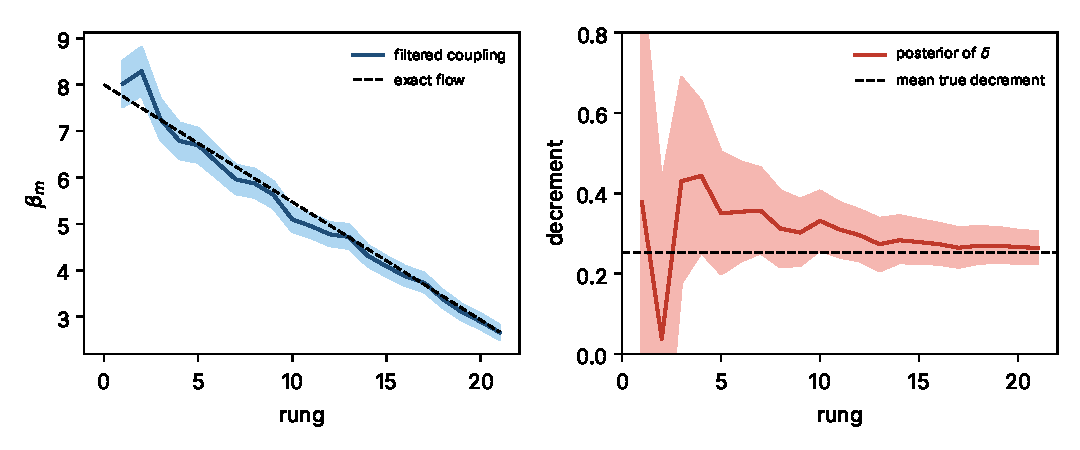
\includegraphics[width=0.85\textwidth]{figures/pl_ladder.pdf}
\caption[Particle learning of the decrement of the ladder]{Particle learning on the ladder with twenty thousand particles and four hundred plaquettes observed at each rung. Left: the filtered coupling with its ninety percent band, against the exact flow. Right: the posterior of the decrement $\delta$ as rungs accumulate, against the mean true decrement.}
\label{fig:plladder}
\end{figure}

We generated data from the exact, unprojected ladder started at $\beta=8$: twenty two rungs, four hundred plaquettes sampled at each. The true decrement varies slowly along the flow, from $0.2527$ to $0.2567$, with mean $0.2537$. Particle learning with twenty thousand particles, the predictive likelihood computed by the delta method, gives after twenty one steps a posterior median of $0.264$ for $\delta$ with ninety percent interval $[0.226,0.304]$ (Figure~\ref{fig:plladder}). Over five seeds the median is $0.261\pm0.004$ (standard error), with ninety percent endpoints $0.223\pm0.005$ and $0.300\pm0.004$; the run shown is seed $0$. Sixty one percent of the particles have distinct parents at the last resampling step; the number of distinct ancestors along the paths, which governs the accumulated sufficient statistics, was not measured, so we claim nothing about degeneracy.

The posterior of the decrement, the beta function at one loop accuracy, comes with an honest interval from data of the kind a simulation produces: twenty two rungs of four hundred plaquettes fix it to fifteen percent. The method does not need the ladder to be the true dynamics, and blocked ensembles from a real simulation would do.

\subsection{Generative Bayesian computation}

Generative Bayesian computation replaces the density of the posterior by a map. Simulate parameters from the prior and data from the model; reduce the data to a statistic; and train a generator, a function of the statistic and of a uniform variable, whose output has the conditional law of the parameter given the statistic. The posterior for observed data is then one forward pass. No likelihood and no partition function is evaluated, only simulations, which is exactly the situation of lattice gauge theory, where simulation is routine and $Z(\beta)$ is out of reach. By Proposition~\ref{prop:suff} nothing is lost if the statistic is sufficient.

We used it for the problem left open in Chapter~\ref{ch:sandwich}: the coupling fitted to a blocked field by pseudolikelihood depended on the blocking rule by a factor of more than three. Matching is the cure, and matching is what a generator trained on simulations does.

\paragraph{\normalfont\scshape Training and validation.} Four hundred and twenty simulations of a $4^4$ lattice, with the protocol of \texttt{gbc\_sim.py}, at couplings drawn uniformly from $[0.3,9]$, each reduced to the plaquette, the $1\times2$ loop and the $2\times2$ loop averaged over sixteen configurations. A gradient boosted quantile regression on the three loops and their logarithms is the generator for the median, trained on three hundred pairs; sixty pairs calibrate a ninety percent interval by split conformal prediction, and sixty test it. Over five replicate trainings and simulations the held out median absolute error in $\beta$ is $0.034\pm0.002$ and the interval covers the truth in $93\pm2$ percent of cases, against a nominal $90$; the coverage of one replicate has a standard error of four.

\paragraph{\normalfont\scshape Application.} Sixteen configurations of an $8^4$ lattice at each of five couplings were blocked to $4^4$ by five rules, plain decimation and decimation with the staples added with weights $0.1$, $0.2$, $0.3$ and $0.5$, and the same three statistics were passed to the generator. The blocked $8^4$ and trained $4^4$ lattices have the same number of sites, so finite size effects are matched, which is Swendsen's two lattice design \cite{Sw79}. As a check that the blocked ensemble is close to a Wilson ensemble we also matched each loop separately; the spread of the three matched couplings measures the distance from the Wilson family.

\begin{center}
\small
\begin{tabular}{cccccc}
\toprule
$\beta$ & smearing & generator, $\beta'$ & 90\% interval & spread of loops & $\beta-\beta'$ \\ \midrule
2.2 & 0.2 & $1.39\pm0.03$ & $[1.34,1.44]$ & $0.12\pm0.01$ & $0.81\pm0.03$ \\
2.5 & 0 & $1.21\pm0.01$ & $[1.17,1.24]$ & $0.51\pm0.01$ & $1.30\pm0.01$ \\
2.5 & 0.2 & $2.13\pm0.02$ & $[2.01,2.25]$ & $0.04\pm0.004$ & $0.38\pm0.02$ \\
2.5 & 0.5 & $2.33\pm0.02$ & $[2.19,2.47]$ & $0.19\pm0.01$ & $0.17\pm0.02$ \\
3 & 0.2 & $2.62\pm0.01$ & $[2.44,2.80]$ & $0.07\pm0.003$ & $0.38\pm0.01$ \\
\bottomrule
\end{tabular}
\end{center}

\begin{figure}[t]
\centering
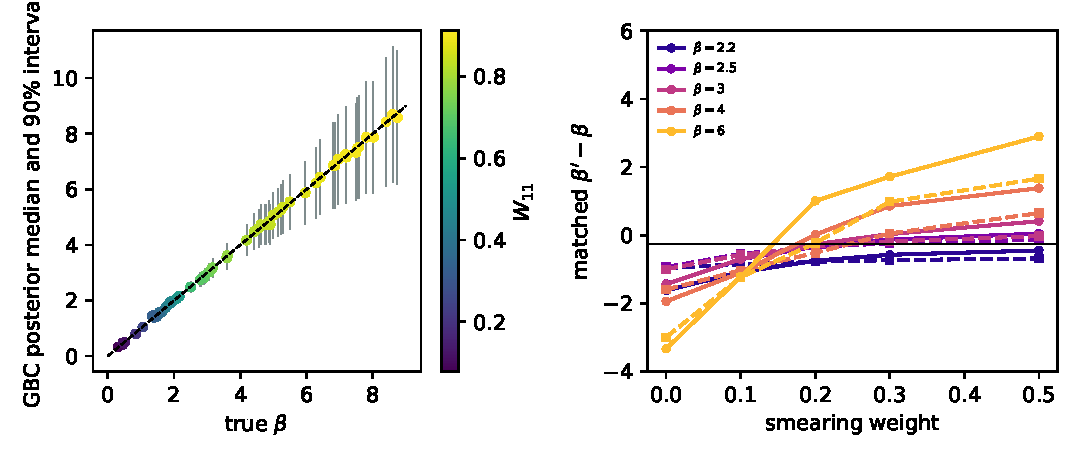
\includegraphics[width=0.85\textwidth]{figures/gbc_match.pdf}
\caption[GBC matching for a blocked lattice]{Left: the generator's posterior median and calibrated ninety percent interval against the true coupling on sixty held out $4^4$ simulations, coloured by the plaquette. Right: the shift $\beta'-\beta$ of the matched coupling of blocked $8^4$ ensembles as a function of the smearing weight of the blocking rule, matched by the plaquette (circles, solid) and by the $2\times2$ loop (squares, dashed); the horizontal line is $-0.26$.}
\label{fig:gbcmatch}
\end{figure}

Three things come out (Figure~\ref{fig:gbcmatch}); each row of the table is the mean over five replicate trainings and simulations, each with a blocked ensemble of sixteen configurations, and the interval column is the mean of the five ninety percent posterior intervals of the generator, which is its posterior uncertainty and not a replicate error. First, the dependence on the blocking rule shrinks: at $\beta=2.5$ pseudolikelihood gave fitted couplings from $0.87$ to $2.81$ across rules, matching gives $1.21$ to $2.33$, and the internal check selects among them, the three loops agreeing to $0.04$ at smearing weight $0.2$ and disagreeing by $0.12$ to $0.51$ at the others, so that the selected ensemble is, to the resolution of three loops, a Wilson ensemble at $\beta'=2.13\pm0.02$ (mean and standard error over the five replicates). Second, the shift at the selected rule is of the right size: $0.38\pm0.02$ at $\beta=2.5$ and $0.38\pm0.01$ at $\beta=3$ (over five replicates), against $0.21$ from the string tension data, $0.27$ from two loop perturbation theory and $0.26$ from the ladder; one step on a $4^4$ lattice with three loops overestimates it by about a half, which Monte Carlo renormalization studies remove with several steps on larger lattices. Third, the method fails gracefully: for $\beta\ge4$ the $4^4$ lattice is deep in its finite volume regime and no rule makes the three loops agree to better than about $0.1$ on average over replicates, which the spread reports.

\subsection{GBC against an exact posterior}

A generator is only as good as its statistic, and the two dimensional lattice lets us say so with numbers, because the posterior there is known in closed form. With $n=256$ independent plaquettes and a uniform prior on $[0.5,6]$, the posterior density of $\beta$ is proportional to $\big(\beta/I_1(\beta)\big)^n e^{n\beta\bar a}$ and depends on the data through the mean $\bar a$ alone. We trained quantile generators on six thousand simulated data sets, once with the sufficient statistic as input and once with the one bit summary, and compared five quantiles with the exact ones on six hundred fresh data sets, from one training run (seed $3$ of \texttt{gbc\_exact.py}), so the quantile errors and widths below carry no replicate error.

\begin{center}
\small
\begin{tabular}{lccc}
\toprule
input & quantile error & 90\% width & coverage \\ \midrule
sufficient statistic & 0.024 to 0.038 & 0.644 & 0.87 \\
one bit summary & 0.119 to 0.135 & 0.808 & 0.91 \\
exact posterior & 0 & 0.653 & 0.905 \\
\bottomrule
\end{tabular}
\end{center}

\begin{figure}[t]
\centering
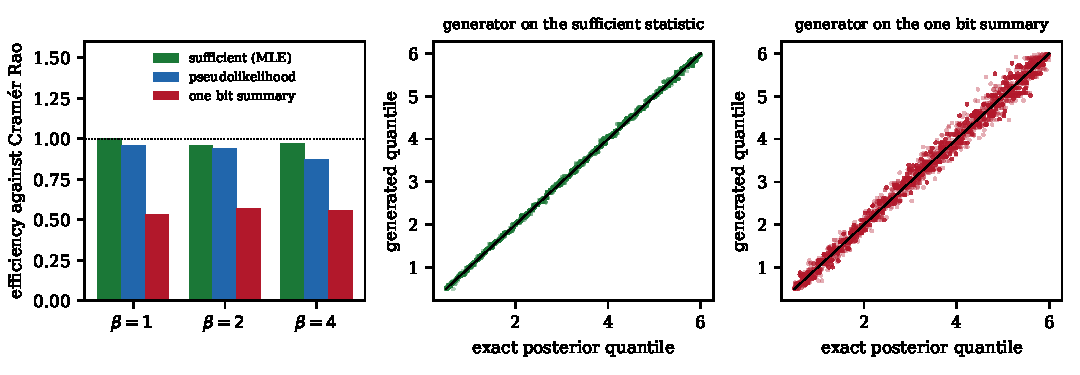
\includegraphics[width=0.85\textwidth]{figures/suff_gbc.pdf}
\caption[Sufficiency, efficiency and GBC]{Left: efficiency of three estimators of the coupling of two dimensional SU(2) against the Cram\'er Rao bound. Centre and right: the fifth, fiftieth and ninety fifth percentiles produced by a quantile generator against the exact posterior percentiles, when the generator is fed the sufficient statistic and when it is fed a one bit summary of each plaquette.}
\label{fig:suffgbc}
\end{figure}

With six hundred test sets a coverage has a standard error of about $0.012$: the exact interval covers $0.905\pm0.012$, the sufficient statistic generator at $0.87$ undercovers by two to three standard errors, and the one bit generator at $0.91$ is not distinguishable from $0.90$. With the sufficient statistic the generator reproduces the exact posterior to about a twentieth of its width; the residual is the training error of a boosted tree and presumably falls with more simulations, which we did not test. With the lossy statistic it is still calibrated and its intervals are a quarter wider. Both facts are general: a generator trained on a statistic $T$ targets the posterior given $T$, which has the right coverage, and what is lost is width, in the proportion that the Fisher information of $T$ falls short. The ratio of widths, $0.808/0.653=1.24$, lies within the range $1/\sqrt{0.67}=1.22$ to $1/\sqrt{0.53}=1.37$ that the efficiency table predicts, the prior truncating both posteriors. The practical rule is that of Proposition~\ref{prop:suff}: feed the generator the loop sums of the action family one is matching to, and nothing coarser (Figure~\ref{fig:suffgbc}).

\subsection{A generator for the gap}

The second role listed at the end of this section, the gap as a parameter, can be tried at once on synthetic correlators. Take $C(\tau)=A_1e^{-m\tau}+A_2e^{-M\tau}$ plus noise at $\tau=1,\dots,10$, with a prior over the gap $m\in[0.2,1.2]$, the amplitudes, the excited level $M-m\in[0.5,2]$ and the noise level between $10^{-3}$ and $10^{-2}$. Six thousand simulated correlators train a quantile generator for $m$; two thousand calibrate its interval; two thousand test it against the effective mass $\log C(\tau)/C(\tau+1)$.

\begin{figure}[t]
\centering
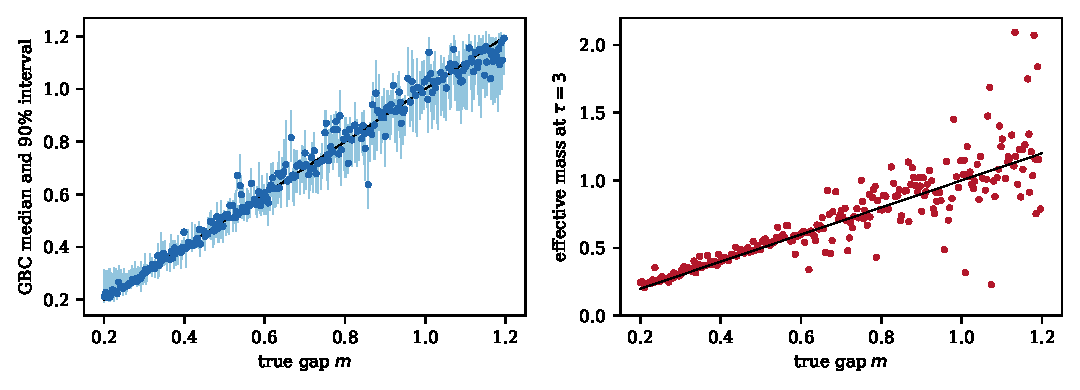
\includegraphics[width=0.85\textwidth]{figures/gbc_gap.pdf}
\caption[A generator for the gap]{Left: the posterior median and calibrated ninety percent interval for the gap produced by a generator trained on simulated two level correlators, against the truth. Right: the effective mass at $\tau=3$ for the same correlators.}
\label{fig:gbcgap}
\end{figure}

The generator's median error is $0.018$, against $0.045$ for the effective mass at $\tau=3$ and $0.091$ at $\tau=5$ (over the $90$ percent of cases in which it is defined); its calibrated ninety percent interval has mean width $0.15$ and covers the truth in $92$ percent of test cases (Figure~\ref{fig:gbcgap}). These are errors over two thousand test correlators from one training run. Over five training runs the median error is $0.0193\pm0.0004$ against $0.0455\pm0.0004$ and $0.097\pm0.003$ for the effective mass at $\tau=3$ and $5$, the interval covers $0.905\pm0.004$ with mean width $0.151\pm0.002$ (standard errors over seeds). The generator uses all ten times with weights learned from the prior, and that is also its limitation: the answer is a posterior under a prior on spectra with two levels, and under a prior that allows a continuum starting at zero no finite set of correlator values bounds the gap below. A generator moves the assumption into the open; it does not remove it.

\subsection{Transformers inside GBC}\index{transformer}\index{attention}

Can a transformer be the generator? A lattice ensemble is a set, and the natural network embeds each element as a token, lets the tokens attend to one another, and pools. By Proposition~\ref{prop:suff} the tokens should be the characters $\chi_n$ of the loops, which makes the network gauge invariant, and by the Pitman Koopman Darmois theorem attention, which can form products of tokens, may be needed once the action leaves the exponential family; with heat kernel weights it may act as a decimation step, and a transformer over plaquette tokens as a learned ladder. With no deep learning library available we tested the two ingredients in their simplest forms, on the two dimensional problem where the posterior is exact.

\paragraph{\normalfont\scshape Pooling.} Each of the $256$ plaquettes is embedded by its characters $\chi_2/2,\dots,\chi_9/9$ and the tokens are averaged, which is attention with uniform weights. A boosted quantile head is trained on the eight pooled coordinates. Only the first is sufficient; the head must find that out.

\paragraph{\normalfont\scshape In context attention.} A single attention head with the test ensemble as query and five thousand simulated ensembles as context: the weight on a context ensemble is $\exp(-\frac12|W(s-s_i)|^2)$ with $s$ the pooled vectors and $W$ diagonal with two free scales, one for the first coordinate and one shared by the other seven, chosen from a grid of twelve pairs on a validation split. The posterior quantiles are the attention weighted quantiles of the context couplings. This is the prior fitted network idea~\cite{MHAGH22} in one layer, and it is a kernel smoother.

The table gives means over five seeds, each with five thousand training and five hundred test sets, the same sets in every row; the standard error of each mean quantile error is about $0.001$, of each width $0.002$ to $0.004$ and of each coverage $0.003$ to $0.006$.

\begin{center}
\small
\begin{tabular}{lccc}
\toprule
generator & quantile error & 90\% width & coverage \\ \midrule
boosted head on the sufficient statistic & 0.026 to 0.038 & 0.648 & 0.88 \\
boosted head on eight pooled characters & 0.032 to 0.050 & 0.656 & 0.88 \\
attention head on eight pooled characters & 0.016 to 0.026 & 0.668 & 0.89 \\
exact posterior & 0 & 0.648 & 0.90 \\
\bottomrule
\end{tabular}
\end{center}

The attention head is the most accurate of the three, but what it chose was partly built in: the grid gave the first coordinate its own scale and the other seven a shared one, so the split between signal and noise was fixed by hand and not learned. Within the grid the validation step chose $0.03$ standard deviations for the first coordinate, the lower end of the grid, and infinity for the shared scale, in all five seeds; to claim that attention finds the sufficient statistic one would have to search eight free scales, which we did not do. The boosted head given the same eight inputs was about thirty percent worse than on the sufficient statistic alone, on the same data sets ($0.040$ against $0.031$); we did not test the natural reason, that it spends splits on the noise coordinates.

So the answer is yes in design and in a toy, with cautions: the toy is an exponential family, where the answer was known, and the case for attention is the blocked ensemble, where no finite statistic is sufficient and a trained network is needed, for which the flows of Kanwar and coauthors \cite{Kan20} and the convolutional networks of Favoni and coauthors \cite{Fav22} are the starting point. A transformer generator inherits every limitation of GBC: it computes posteriors under a simulated prior and proves nothing.

\subsection{Are GBC methods useful?}

Yes, for computation and for diagnosis, in three roles. Amortised matching: a generator trained once on small lattice simulations turns any blocked ensemble into a posterior for its effective coupling in a forward pass (twenty five posteriors in under a second, from about four minutes of parallel simulation), and extended to the character coefficients of a plaquette law it is the empirical ladder that Chapter~\ref{ch:sandwich} asked for. The gap as a parameter: a generator trained on simulated correlators with known spectra would give the posterior of the estimator of Chapter~\ref{ch:estimation} instantly and make the dependence on the prior over spectra explicit. Learning the block spin map: a generator trained on pairs of fine and blocked summaries is a learned ladder, which would show where in the bracket the truth lies for any blocking rule.

For a proof they are not useful directly: a trained generator is not a theorem, and its guarantees, such as the Bernstein von Mises transfer of our Hilbert sixth book \cite{PS26h}, concern statistical accuracy and not rigour of bounds. Their indirect use is real, though. The comparison problem needs a blocking rule and a pair of brackets, and there are infinitely many candidates. A learned ladder is a fast way to search that space for a rule under which the blocked law stays in a low dimensional family and the sandwich holds with room to spare, before any attempt is made to prove it. The pooled character model of the transformer experiment is of the kind suggested by quantum Bayesian computation \cite{PSX23}; Section~\ref{ch:quantum} takes the question up.

\section{Quantum Bayesian Computation and the Gap}\label{ch:quantum}\index{quantum Bayesian computation}\index{von Neumann measurement}\index{quantum Fourier transform}\index{Kogut Susskind Hamiltonian}

The mass gap is an eigenvalue difference. Monte Carlo infers it from a decay; a quantum computer would measure it. This section asks what our work on quantum Bayesian computation gives the problem, and what it gives the classical computations of this chapter as an architecture.

\subsection{Von Neumann's principle}

Our paper with Jianeng Xu \cite{PSX23} organises Bayesian computation round von Neumann's principle of measurement: a quantity of interest is written as $\operatorname{tr}(\rho\,Q)$ for a density operator $\rho$ and an observable $Q$, and is obtained by evolving a physical system and measuring it. Data enter through a feature map $x\mapsto\rho(x)$ into density matrices, a model is $f_W(x)=\operatorname{tr}(\rho(x)W)$, the kernel is $k(x,x')=\operatorname{tr}(\rho(x)\rho(x'))$, and since the model is linear in $W$, fitting $W$ is a convex problem, whose solution by the representer theorem lies in the span of the $\rho(x_i)$.

In most of statistics the trace formula is an analogy. In lattice gauge theory it is the definition. By reflection positivity a correlation on a lattice of temporal extent $N_t$ is
\[
\langle O_1(0)O_2(k)\rangle=\frac{\operatorname{tr}\big(\mathcal T^{N_t-k}O_1\,\mathcal T^kO_2\big)}{\operatorname{tr}\mathcal T^{N_t}},\qquad \mathcal T=e^{-H},
\]
with $\mathcal T$ the transfer operator, and the mass gap is the difference of the two lowest eigenvalues of $H$. The estimation problem of the earlier chapters, the gap from the decay of a correlator, is the classical shadow of a measurement of that difference. So of all the problems to which the methods of \cite{PSX23} apply, this is one where the quantum formulation is native and not a translation.

\subsection{One plaquette as a quantum system}\label{sec:oneplaquette}

The smallest example can be solved, and it shows the two regimes of the full problem. In the Hamiltonian formulation of Kogut and Susskind \cite{KS75} a single plaquette of SU(2), restricted to gauge invariant states, which are class functions, has
\[
H_\lambda=-\lambda\,\Delta+\frac1\lambda\,(1-\cos\theta),
\]
with $\Delta$ the Laplacian of this book, whose eigenvalue on the character $\chi_n$ is $-\frac14(n^2-1)$, and $\lambda$ proportional to the square of the coupling, with a constant fixed by the normalisation of the Hamiltonian.

\begin{proposition}[one plaquette]\label{prop:oneplaquette}
In the orthonormal basis $\chi_1,\chi_2,\dots$ of class functions the operator $H_\lambda$ is the tridiagonal matrix with diagonal entries $\frac14\lambda(n^2-1)+1/\lambda$ and off diagonal entries $-1/2\lambda$. Its gap is $\frac34\lambda+O(1/\lambda^3)$ as $\lambda\to\infty$ and tends to $\sqrt2$ as $\lambda\to0$.
\end{proposition}

\begin{proof}
The Casimir is diagonal, and $\cos\theta\,\chi_n=\frac12(\chi_{n+1}+\chi_{n-1})$ with $\chi_0=0$, since $\chi_2\chi_n=\chi_{n+1}+\chi_{n-1}$. For large $\lambda$ the potential is a bounded perturbation of the Casimir, whose lowest levels are $0$ and $\frac34\lambda$; the first order shifts of the two levels are equal, both $1/\lambda$ since $\cos\theta$ has no diagonal entries, and the second order shifts are of order $\lambda^{-2}$ over a level spacing of order $\lambda$. For small $\lambda$ the ground state concentrates at the identity, where $1-\cos\theta=\frac12\theta^2$ and $-\Delta$ is a quarter of the Laplacian of $\mathbb R^3$ in the length $\theta$; the operator $\frac14\lambda\,p^2+q^2/2\lambda$ is a harmonic oscillator of frequency $1/\sqrt2$, and the first excited radial state lies two quanta above the ground state.
\end{proof}

So the gap of one plaquette is never small: it is $\frac34\lambda$ at strong coupling, where it is the first Casimir, the number that appears all through this book, and $\sqrt2$ at weak coupling, with a minimum near $1.1$ between. Table~\ref{tab:oneplaquette} and Figure~\ref{fig:quantumplaquette} give the numbers. A single plaquette has no infrared problem; the problem of four dimensions is that infinitely many of them share links.

\begin{table}[t]
\centering\small
\begin{tabular}{rcccc}
\toprule
$\lambda$ & gap & $\frac34\lambda$ & characters kept & count of ground state \\ \midrule
$8$ & $6.0009$ & $6.0000$ & $3$ & $0.04$ \\
$2$ & $1.5569$ & $1.5000$ & $5$ & $0.75$ \\
$1$ & $1.0982$ & $0.7500$ & $6$ & $3.09$ \\
$0.5$ & $1.2394$ & $0.3750$ & $9$ & $8.78$ \\
$0.1$ & $1.3824$ & $0.0750$ & $20$ & $54.06$ \\
$0.02$ & $1.4079$ & $0.0150$ & $46$ & $280.34$ \\
\bottomrule
\end{tabular}
\caption[One plaquette in the Hamiltonian formulation]{The gap of $H_\lambda$, the number of characters that must be kept for the gap to be right to $10^{-8}$, and the count $E[1/(1-\cos\theta)]-2$ of the ground state density. The weak coupling limit of the gap is $\sqrt2=1.4142$.}
\label{tab:oneplaquette}
\end{table}

\begin{figure}[t]
\centering
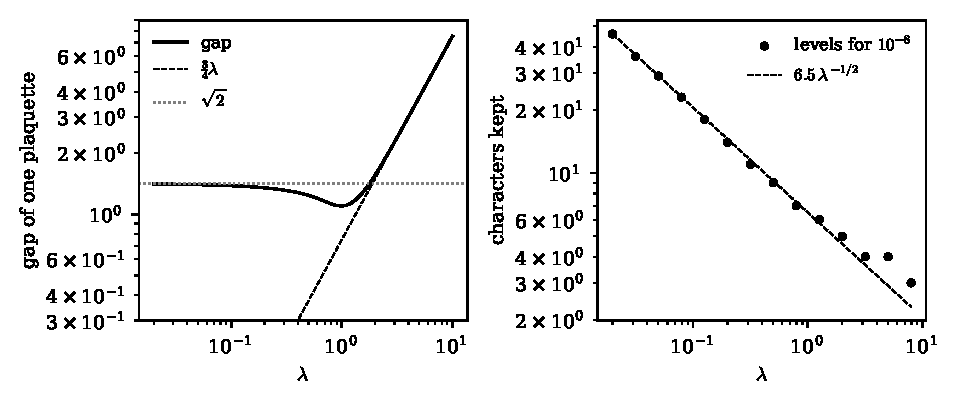
\includegraphics[width=0.85\textwidth]{figures/quantum_plaquette.pdf}
\caption[The gap and the truncation of one plaquette]{Left: the gap of one plaquette against $\lambda$, with its strong coupling asymptote $\frac34\lambda$ and its weak coupling limit $\sqrt2$. Right: the number of characters needed for an error of $10^{-8}$ in the gap, against $6.5\,\lambda^{-1/2}$.}
\label{fig:quantumplaquette}
\end{figure}

\paragraph{\normalfont\scshape Truncation and the count.} A quantum simulation keeps finitely many levels on each link, and the table says how many: at weak coupling the number of characters needed grows like $6.5\,\lambda^{-1/2}$ for eight figures. The count of Proposition~\ref{prop:observable} on the square of the ground state (in its class by Corollary~\ref{cor:vacuumcount}) agrees with $4\sqrt2/\lambda-\frac52$ to $0.003$ for $\lambda\le0.05$ (a numerical fit; the leading term is the harmonic oscillator value), so the levels a link needs grow like the square root of its count, about $2.7\sqrt M$. The latent count of Chapter~\ref{ch:counts}, introduced as a mixing variable and found to be an observable, is here also the measure of the register a link requires.

\subsection{The vacuum of one plaquette has real zeros}\label{sec:vacuumzeros}

The transfer operator of the plaquette over a short time $\epsilon$ is, by Trotter's formula, a heat flow between two multiplications,
\[
T_\epsilon=e^{-\epsilon V/2}\,e^{\epsilon\lambda\Delta}\,e^{-\epsilon V/2},\qquad V=\frac1\lambda(1-\cos\theta),
\]
and each factor is one of the operations of Chapter~\ref{ch:zeros}. That has a consequence for the vacuum.

\begin{proposition}[the vacuum has real zeros]\label{prop:vacuumzeros}
The ground state $\psi_0$ of $H_\lambda$, as an entire function of $x=\cos\theta$, has only real zeros, all in $(-\infty,-1]$. Hence
\[
\psi_0(x)=\psi_0(0)\,e^{ax}\prod_m\Big(1+\frac{x}{\gamma_m}\Big),\qquad a\ge0,\ \gamma_m\ge1,
\]
and $\psi_0(0)/\psi_0(x)$ is the Laplace transform in $x$ of a generalized gamma convolution with drift $a$ and unit Thorin atoms at the $\gamma_m$. The same holds for the vacuum density $\psi_0^2$, with atoms of weight two.
\end{proposition}

The proof needs one estimate, uniform in the Trotter step. In the character basis write $X$ for multiplication by $\cos\theta$, the tridiagonal matrix with entries $\frac12$, put $\kappa=\epsilon/2\lambda$, and write
\[
T_\epsilon=M\,D\,M,\qquad M=e^{\kappa(X-1)},\qquad D=\operatorname{diag}\big(e^{-\epsilon\lambda(n^2-1)/4}\big).
\]

\begin{lemma}[domination]\label{lem:domination}
For $m\epsilon=s$ every entry of $T_\epsilon^m$ satisfies
\[
0\le\big(T_\epsilon^m\big)_{nj}\le b_n(s)=e^{-s\lambda(n^2-4)/16}+e^{s/\lambda}\,\frac{(s/\lambda)^{\lceil n/2\rceil}}{\lceil n/2\rceil!},
\]
and every row sum is at most $1$. If $c\ge0$ is a unit vector with $T_\epsilon c=\mu c$, then $c_n\le\mu^{-m}\,b_n(s)^{1/2}$.
\end{lemma}

\begin{proof}
All of $X$, $M$ and $D$ have nonnegative entries, and $X$ has row sums at most $1$, so the same is true of $M$ and of $T_\epsilon$. Expand each factor $M$ in powers of $X$: the entry $(n,j)$ of $T_\epsilon^m$ becomes a sum over nearest neighbour paths from $j$ to $n$, each step with weight $\frac12$, interleaved with the diagonal factors. Paths that stay at or above level $n/2$ collect from each of the $m$ factors $D$ at most $e^{-\epsilon\lambda(n^2/4-1)/4}$, and the rest of their weight is an entry of $e^{2m\kappa(X-1)}$, which is at most $1$. Paths that go below $n/2$ have at least $\lceil n/2\rceil$ steps; dropping the factors $D$, which are at most $1$, the total weight of paths with $r$ steps is at most $(2m\kappa)^r/r!$, and $2m\kappa=s/\lambda$. Summing over $r\ge\lceil n/2\rceil$ gives the second term. For the eigenvector, $c=\mu^{-m}T_\epsilon^mc$ and, by the Cauchy and Schwarz inequality, $\sum_j(T_\epsilon^m)_{nj}c_j\le\big(\sum_j(T_\epsilon^m)_{nj}^2\big)^{1/2}\le\big(\max_j(T_\epsilon^m)_{nj}\big)^{1/2}$, the row sum being at most $1$.
\end{proof}

\begin{proof}[Proof of Proposition~\ref{prop:vacuumzeros}]
The constant function is in $\mathcal L$. Multiplication by $e^{\kappa x}$ is a limit of multiplications by $(1+x/\gamma)^m$ with $\gamma=m/\kappa\ge1$, and $\mathcal L$ is closed under products; the heat flow preserves $\mathcal L$ by Theorem~\ref{thm:zeros}. So every $T_\epsilon^k1$ is a locally uniform limit, in the complex variable $x$, of members of $\mathcal L$.

A function $\sum_nc_n\chi_n$ with $c_n\ge0$ is bounded on the ellipse through $\cosh\tau$ with foci $\pm1$ by its value $\sum_nc_n\sinh(n\tau)/\sinh\tau$ at $\cosh\tau$, since $\chi_n(\cos\theta)=\sum_ke^{i(n-1-2k)\theta}$. By Lemma~\ref{lem:domination} with $s=1$ the coefficients of the normalised iterates $T_\epsilon^k1/\|T_\epsilon^k1\|$, for $k\ge1/\epsilon$, and of the ground state $\phi_\epsilon$ of $T_\epsilon$, are bounded by a constant times $b_n(1)^{1/2}$, uniformly in $k$ and in $\epsilon\le1$: the factor $\mu^{-m}$ is $e^{E_\epsilon}$ with $E_\epsilon$ bounded, and for the iterates the ratio $\|T_\epsilon^{k-m}1\|/\|T_\epsilon^k1\|$ is bounded because the iterates keep an overlap with $\phi_\epsilon$ that is bounded below. Since $b_n(1)^{1/2}$ decays faster than any exponential, these families are uniformly bounded on every compact set of the $x$ plane, hence normal. The iterates converge in $\ell^2$ to $\phi_\epsilon$, because $T_\epsilon$ is compact, positivity improving and has a simple top eigenvalue; and $\phi_\epsilon\to\psi_0$ in $\ell^2$ as $\epsilon\to0$ by Trotter's formula and the simplicity of the ground state of $H_\lambda$. A normal family with convergent coefficients converges locally uniformly, and Hurwitz's theorem gives $\psi_0$ only real zeros, all in $(-\infty,-1]$. An entire function that is such a limit of polynomials with zeros on a half line has the displayed form, by the theorem of Laguerre and P\'olya; and the reciprocal of $e^{ax}\prod(1+x/\gamma_m)$ is the Laplace transform of a drift plus a sum of independent exponential variables.
\end{proof}

As a check on the conclusion, independent of the proof: with the ground state computed to $160$ digits (\texttt{vacuum\_zeros.py}) in a basis of $70$ to $110$ characters, the number of zeros in a disc, counted by the argument principle, equals the number of sign changes on the real axis below $-1$: one zero in $|x|<12$ at $\lambda=2$, at $x=-6.731$; five in $|x|<6$ at $\lambda=\frac12$, the nearest at $-1.206$; fifteen in $|x|<2.5$ at $\lambda=\frac1{10}$, the nearest at $-1.0065$. At $60$ digits the last count comes out wrong, a warning of the kind recorded in Chapter~\ref{ch:zeros}.

\begin{corollary}\label{cor:vacuumcount}
The vacuum density $\psi_0^2$ of one plaquette is a mixture $\sum_j\pi(j)f_j$ with a log concave count law $\pi$, whose mean is the count of Table~\ref{tab:oneplaquette}.
\end{corollary}

\begin{proof}
$\psi_0^2$ is in the closure of $\mathcal L$, and Proposition~\ref{prop:Llogconcave} and Proposition~\ref{prop:observable} pass to limits.
\end{proof}

So the vacuum of the smallest gauge system belongs to the class in which the heat kernel lives, with zeros that crowd toward the antipode as the coupling weakens, and its reciprocal has the Thorin form on which this book began. The proof used nothing about the potential except that $e^{-\epsilon V}$ is, up to a constant, a Wilson weight; whether the same holds for other single plaquette actions whose Boltzmann factor is in the closure of $\mathcal L$, the heat kernel action among them, is not shown here. For several plaquettes the statement to aim at is the same one, in each plaquette variable separately, and that is a question about how sharing a link interacts with real zeros: Conjecture~\ref{conj:Lclosed} is the case of two.

\subsection{The ladder alternates between two bases}

The two halves of a rung are diagonal in different bases: decimation is a convolution, diagonal in characters ($u_n\mapsto u_n^{\,p}$), and bond moving a pointwise product, diagonal in the group variable, with the matrix $u_n(j+1)$ of Chapter~\ref{ch:counts} as the change of basis between counts and characters. That is the pattern of the quantum Fourier transform models of \cite{PSX23}: layers each trivial in their own basis, joined by a fixed transform. Nothing in the ladder needs a quantum computer, since it is a commutative computation; the noncommutative one is the lattice $\mathbb Z^4$, where a plaquette shares each of its links with five others, and the comparison problem of Chapter~\ref{ch:sandwich} asks how far the true blocking map is from one that is diagonal in alternate bases.

\subsection{Band limited models as an architecture for GBC}

A model $\operatorname{tr}(\rho(x)W)$ with a fixed encoding is a finite Fourier series in the data. For a gauge invariant model of a lattice gauge field the Peter and Weyl theorem says it is a combination of characters $\chi_n$ of plaquettes and longer loops up to a band $N$, and the coherent state kernel, Gaussian in \cite{PSX23}, is on the group the heat kernel $K_t(UV^{-1})$, positive definite because its character coefficients are positive. So the quantum architecture, run on a classical machine, is: Peter and Weyl features to a band $N$, pooled over the lattice; products of a few copies of the pooled vector, which is what several copies of the state give; and a linear readout fitted by ridge regression, a convex problem.

We tried it on the test problem of Section~\ref{ch:plgbc}: $256$ independent Wilson plaquettes, a uniform prior on $\beta$, and the exact posterior median as the target. The readout is a quadratic polynomial in the pooled characters plus the cube of the first, fitted on $4000$ simulated sets and tested on $500$.

\begin{center}
\small
\begin{tabular}{lcccc}
\toprule
band $N$ & $1$ & $2$ & $4$ & $8$ \\ \midrule
features & $4$ & $7$ & $16$ & $46$ \\
error against the exact median & $0.040$ & $0.033$ & $0.031$ & $0.035$ \\
\bottomrule
\end{tabular}
\end{center}

The error is the mean absolute one, from one seed, so differences in the third decimal are not resolved. The first character is sufficient for this model, so in principle band $1$ is enough, and the small gain from bands $2$ and $4$ is the polynomial readout borrowing nonlinearity from the higher characters; at band $8$ the extra features begin to cost. The attention head of Section~\ref{ch:plgbc}, at $0.016$ at the median, does better than any of these; the boosted head on the same pooled characters, at $0.032$, does not. The comparison is between different training sets ($4000$ against $5000$) with the same $n$ and prior. So against the attention head the convex readout is the limiting factor here and not the features. The advice that survives is about the feature layer: put the invariance and the band limit into the encoding, where the theory says what they are, and spend the flexibility on the readout. The paper notes that convex training avoids the flat landscapes met by deep parameterised circuits; the experiment says that on this problem one pays for the convexity with up to a factor of two in error.

\subsection{What a quantum computer could and could not do}

\paragraph{\normalfont\scshape Could.} Evolve a truncated Kogut and Susskind Hamiltonian and read the gap as a phase. Phase estimation \cite{Ki95}, a standard result of quantum computation, to precision $\varepsilon$ needs evolution for a time of order $1/\varepsilon$, so a gap $m$ is resolved in time of order $1/m$, against the classical need for correlators at separations of several $1/m$ with noise that does not fall with the signal. Real time evolution and matter at finite density, where Monte Carlo has a sign problem, are the cases usually argued for.

\paragraph{\normalfont\scshape Could not.} Prove a gap. The ground state must be prepared, and adiabatic preparation \cite{FGGS00}, by the adiabatic theorem, takes a time that grows as an inverse power of the gap along the path, so the cost of the measurement depends on the quantity measured; at weak coupling the gap in lattice units is expected, from asymptotic freedom, to be exponentially small in $\beta$ and the lattice must be exponentially large. And a measurement at finite volume and finite truncation is a number with an error bar, the same kind of evidence as a lattice simulation. For the Euclidean theory without matter Monte Carlo has no sign problem and is efficient; no speed up is claimed for anything in this book. Our later paper with Zantedeschi \cite{PSZ26} ties the Born rule and Bayes's rule together through noncommutativity, with reflection positivity as its Euclidean trace; we have not used the connection beyond this remark.

\subsection{Open problems}

\begin{problem}\label{op:twoplaquettes}
Two plaquettes sharing a link, in the Hamiltonian formulation and restricted to gauge invariant states. Is the vacuum, as a function of each plaquette variable $\cos\theta_p$ with the other held fixed, an entire function with only real zeros below $-1$? This is the Hamiltonian form of Conjecture~\ref{conj:Lclosed}; the difficulty is that the heat flow on the shared link acts on both variables at once.
\end{problem}

\begin{problem}\label{op:registers}
Prove the rule for registers: that the number of characters needed to compute the gap of one plaquette to a fixed accuracy is asymptotic to a constant times the square root of the count of the vacuum as $\lambda\to0$, and find the constant as a function of the accuracy. Lemma~\ref{lem:domination} gives an upper bound of order $\lambda^{-2/3}$ for the vacuum itself, weaker than this shape.
\end{problem}

\begin{problem}\label{op:vacuumthorin}
The Thorin atoms $\gamma_m(\lambda)$ of the vacuum decrease toward $1$ as $\lambda\to0$: the nearest is at $6.731$, $1.206$ and $1.0065$ for $\lambda=2$, $\frac12$ and $\frac1{10}$. Show that each is monotone in $\lambda$, the analogue of the monotonicity in $t$ of the zeros of the heat kernel on which the contraction theorem rests.
\end{problem}

\subsection{Assessment}

Useful in three ways, none of them a step toward a proof. The principle of measurement names what the gap is and why its estimation from Euclidean data is indirect; the alternation of bases is the cleanest description of the ladder and of what the lattice lacks; and the band limited encoding is a sound feature layer for GBC on gauge fields, with a convex readout as a baseline that costs up to a factor of two against the attention head. The one plaquette computation adds a rule for registers: the levels a link needs grow like the square root of its count.

We read \cite{PSX23} in full up to the start of its application section and \cite{PSZ26} in abstract only.

\section*{Exercises}
\begin{enumerate}
\item Prove Theorem~\ref{thm:hitgap}(i) for a reversible Markov chain in discrete time with a positive transition operator, and deduce the bound on $1-e^{-m}$ stated in the text.
\item For Brownian motion on SU(2), find the limiting hazard rate of the hitting time of the cap $\{\theta\ge\alpha\}$, check that the bound of Theorem~\ref{thm:hitgap}(i) holds for every $\alpha$, and find the $\alpha$ at which it is tightest.
\item Show that the quadratic match of Remark~\ref{rem:cramerloop} gives $(1-1/k)^2t^2/36$ at second order, compare it with the second order coefficient of Theorem~\ref{thm:expansion}, and ask how much of the difference the quartic term $\theta^4/180$ of $\log(\theta/\sin\theta)$ can account for.
\item (Section~\ref{ch:plgbc}) Show that the Fisher information for $\beta$ in the Wilson measure is $\partial_\beta^2\log Z$, and evaluate it for one plaquette in two dimensions.
\item (Section~\ref{ch:plgbc}) Show that $I_3(\kappa)/I_1(\kappa)=(I_2(\kappa)/I_1(\kappa))^{8/3}$ has no solution with $\kappa>0$.
\item (Section~\ref{ch:plgbc}) Write the particle learning step for the ladder with the heat kernel observation model and verify that the sufficient statistics update as stated.
\item (Section~\ref{ch:quantum}) Verify $\cos\theta\,\chi_n=\frac12(\chi_{n+1}+\chi_{n-1})$ and write $H_\lambda$ for $N=3$. Find its gap at $\lambda=8$ and compare with Table~\ref{tab:oneplaquette}.
\item (Section~\ref{ch:quantum}) Show that the substitution $\psi=\Omega\sin\theta$ turns $H_\lambda\Omega=E\Omega$ into a Mathieu equation, and recover the weak coupling limit $\sqrt2$ of the gap.
\item (Section~\ref{ch:quantum}) For two plaquettes sharing a link, restricted to gauge invariant states, write the Hamiltonian in a basis of pairs of characters. Which term fails to be diagonal in either the character or the group basis?
\end{enumerate}

\part{Exact Models}
\chapter{Two Dimensions and Other Exact Models}\label{ch:twod}

Chapter~\ref{ch:hitting} ended with methods that learn the gap from samples. Those methods are tested, and the theory behind them is calibrated, on the worlds where everything can be computed. This chapter collects them: two dimensional Yang Mills theory, where the gap is a statement about Brownian motion on a compact group (Section~\ref{sec:su2bm}) and a guided tour of the whole method in that case (Section~\ref{ch:tour}); Riemann's kernel on the three sphere (Section~\ref{ch:riemann}); dynamic and static gaps (Section~\ref{ch:dynamic}); the renormalization group (Section~\ref{ch:rg}); free fields (Section~\ref{ch:freefield}); and large $N$ (Section~\ref{ch:largeN}). None of them is four dimensional Yang Mills. Each shows what an exact answer looks like, and the chapters on the ladder put back what is missing.

\section{Brownian Motion on SU(2)}\label{sec:su2bm}

In two dimensions Yang Mills theory can be solved exactly, on the lattice~\cite{Mi75} and in the continuum~\cite{GKS89,Se97,Le03}, and the solution is a statement about Brownian motion\index{Brownian motion on SU(2)} on a compact group. This section works out that statement for SU(2) and proves the uniform Thorin gap inequality of Section~\ref{ch:routeB} from the coarsest lattice all the way to the continuum.

\subsection{Brownian motion on the three sphere}

The group SU(2) consists of matrices $\begin{pmatrix}a&-\bar b\\ b&\bar a\end{pmatrix}$ with $|a|^2+|b|^2=1$, so it is the unit sphere $S^3\subset\mathbb C^2$. Every element is conjugate to $\operatorname{diag}(e^{i\theta},e^{-i\theta})$ for a unique rotation angle $\theta\in[0,\pi]$, which is the geodesic distance from the identity. Class functions depend only on $\theta$, and the Haar measure\index{Haar measure} pushes forward to the density $\frac2\pi\sin^2\theta$ on $[0,\pi]$.

The irreducible representations are indexed by their dimension $n=1,2,3,\dots$, with characters
\[
\chi_n(\theta)=\frac{\sin n\theta}{\sin\theta}
\]
and Casimir\index{Casimir} eigenvalues $(n^2-1)/4$. With the Laplacian normalised so that these are the eigenvalues, Brownian motion on SU(2) started at the identity has, at time $t$, the density with respect to Haar measure
\[
K_t(\theta)=\sum_{n\ge1}n\,e^{-t(n^2-1)/4}\,\chi_n(\theta).
\]
Three readings of this formula will be used repeatedly.
\begin{enumerate}
\item[(i)] The character coefficients $u_n(t)=e^{-t(n^2-1)/4}$ are the Fourier transform of the law of the Brownian position, and the Casimir is its Laplace exponent. Convolution of laws multiplies Fourier coefficients, so $K_t*K_{t'}=K_{t+t'}$: Brownian times add.
\item[(ii)] The smallest nonzero Laplace exponent is $3/4$. It is the spectral gap of the Laplacian on $S^3$ in this normalisation, and the exponential rate at which Brownian motion on SU(2) forgets its starting point and approaches the Haar law.
\item[(iii)] For small $t$, Poisson resummation gives the image sum
\[
K_t(\theta)\propto t^{-3/2}e^{t/4}\sum_{m\in\Z}\frac{\theta+2\pi m}{\sin\theta}\,e^{-(\theta+2\pi m)^2/t},
\]
dominated by $m=0$: $K_t(\theta)\approx c\,t^{-3/2}\,\frac{\theta}{\sin\theta}\,e^{-\theta^2/t}$. The factor $\theta/\sin\theta$ is $j^{-1/2}$, the inverse square root of the Jacobian $j=(\sin\theta/\theta)^2$ of the exponential map (Section~\ref{sec:jacobian}). It is the only trace of curvature at short times, and it will carry asymptotic freedom\index{asymptotic freedom} in Section~\ref{ch:mk}.
\end{enumerate}

\begin{figure}[t]
\centering
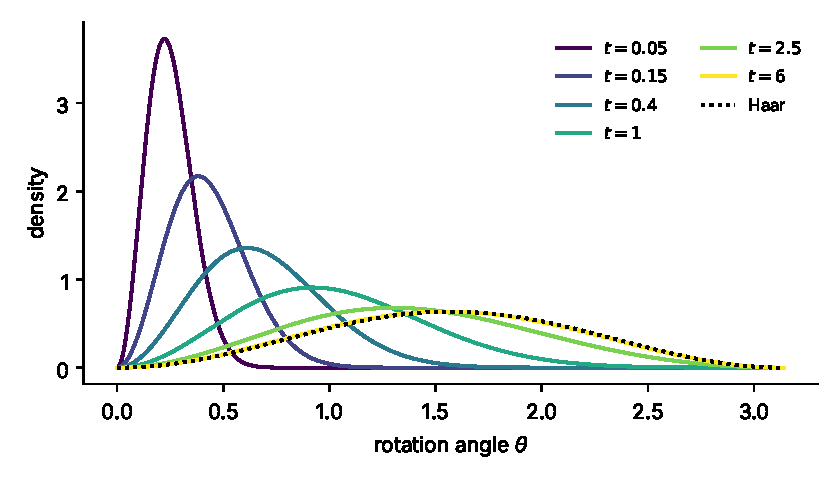
\includegraphics[width=0.92\textwidth]{figures/heat_kernel_laws.pdf}
\caption[Laws of the rotation angle of Brownian motion on SU(2) at several times, against the Haar law]{Laws of the rotation angle of Brownian motion on SU(2) at several times, against the Haar law. At small times the law is a three dimensional Gaussian in disguise; at large times it relaxes to Haar at the rate $3/4$ set by the first Casimir.}
\label{fig:hklaws}
\end{figure}

\subsection{The continuum theory on a surface}

Migdal~\cite{Mi75} discovered, and Witten~\cite{Wi91} later explained in geometric terms, that two dimensional Yang Mills theory on a closed surface $\Sigma$ of genus $h$ and area $A$ has partition function
\[
Z_h(A)=\sum_R(\dim R)^{2-2h}\,e^{-A\,C_2(R)/2},
\]
with the coupling absorbed into the area. For SU(2) this is
\[
Z_h(A)=\sum_{n\ge1}n^{2-2h}\,e^{-A(n^2-1)/8}.
\]
The theory has no local degrees of freedom; its only invariant is the area (the normalisation of $Z_h$ is fixed only up to a factor $e^{cA}$~\cite{Wi91}; rigorous constructions are in~\cite{Se97,Le03}). For every genus the partition function is completely monotone in $A$, since all the weights $n^{2-2h}$ are positive, with spectral measure\index{spectral measure} $\sum_{n\ge2}n^{2-2h}\delta_{(n^2-1)/8}$ after the trivial representation is removed. Area plays the role of Euclidean time, and the gap is $3/8$. Theorem~\ref{thm:rateB} applies verbatim with area in place of time (Figure~\ref{fig:2dgapB}).

The Route B Thorin density\index{Thorin density} has an especially clean form here. On the torus it is $\psi_A(y)/(\pi y)$, where $\psi_A(y)=Z(A)-\operatorname{Re}Z(A+iy)$ with the vacuum removed, and $Z(A+iy)$ is a Jacobi theta function at complex modulus. It is periodic in the real time $y$, with period $16\pi$, because $n^2-1$ is an integer.

\begin{figure}[t]
\centering
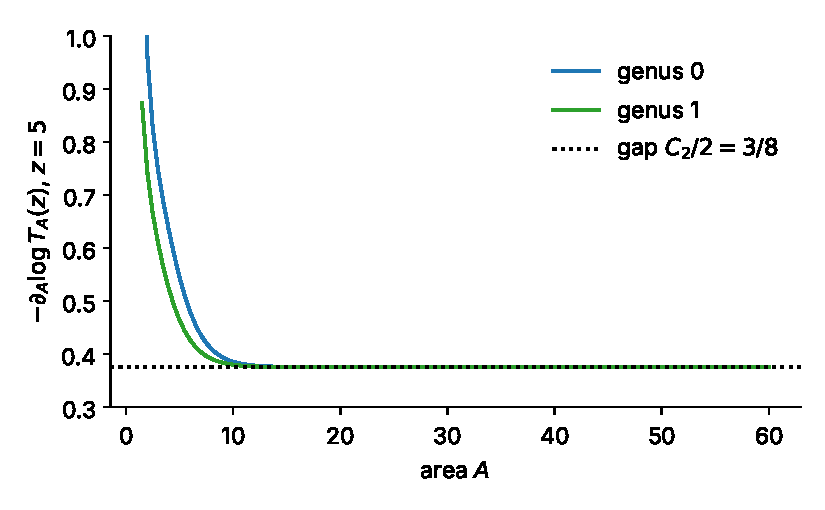
\includegraphics[width=0.8\textwidth]{figures/ym2d_gap.pdf}
\caption[Two dimensional SU(2) Yang Mills on the sphere and the torus: the local Thorin decay rate in area]{Two dimensional SU(2) Yang Mills on the sphere and the torus: the local Thorin decay rate in area converges to the Casimir gap $3/8$.}
\label{fig:2dgapB}
\end{figure}

\subsection{The lattice theory and exact decimation}

On the lattice the key fact is that decimation\index{decimation} is exact in two dimensions. Gluing two adjacent plaquettes along a common link and integrating out that link convolves their weights as class functions. In character variables this multiplies the coefficients:
\[
(f*g)\;\longleftrightarrow\;u_n(f)\,u_n(g).
\]
A block of $b\times b$ plaquettes therefore has weight with coefficients $u_n^{\,b^2}$. For the heat kernel\index{heat kernel} action, $u_n^{b^2}=e^{-b^2t(n^2-1)/4}$, which is again a heat kernel with $t$ multiplied by $b^2$. The heat kernel action is the fixed form of exact decimation, and the parameter $t$ is the area measured in units of the coupling.

Place the theory on a cylinder whose spatial circle has $L$ sites and physical length $\ell$, so the lattice spacing is $a=\ell/L$. For SU(2) the Wilson coupling is $\beta=4/(g^2a^2)$. Physical states are class functions of the holonomy around the circle, and one time step glues a ring of $L$ plaquettes. The transfer matrix\index{transfer matrix} is therefore diagonal in characters, with eigenvalues $u_n(\beta)^L$ where $u_n=I_n/I_1$. In physical units the gauge invariant spectrum is
\[
E_n(a)=-\frac{L}{a}\log u_n(\beta)=-\frac{g^2\ell\beta}{4}\log u_n(\beta),\qquad n\ge1,
\]
with $E_1=0$ the vacuum. Because $I_\nu(\beta)$ decreases in $\nu$, the gap of the whole theory is $\Delta(a)=E_2(a)$. As $a\to0$ the Bessel asymptotics give $u_n=1-(n^2-1)/(2\beta)+O(\beta^{-2})$, so $E_n\to\frac{g^2\ell}{2}\cdot\frac{n^2-1}{4}$, the Casimir spectrum, with continuum gap
\[
\Delta_{\mathrm{cont}}=\frac{3g^2\ell}{8}.
\]
The gap grows linearly with the length of the circle. That is confinement\index{confinement}: the energy of a flux tube wrapping the circle grows with its length. In two dimensions there are no propagating gluons, so this gap is a string tension rather than a particle mass. The point of the exercise is not the physics of two dimensions but the mechanism of the proof, which we now give.

\subsection{A uniform gap from a Bessel inequality}

\begin{lemma}[Bessel ratio bound]\label{lem:amosB}
For all $\beta>0$, $-\log u_2(\beta)\ge\operatorname{arcsinh}\big(\tfrac{3}{2\beta}\big)$.
\end{lemma}

\begin{proof}
Amos\index{Amos, D. E.}'s inequality~\cite{Am74}, valid for $\nu\ge0$, $I_{\nu+1}(\beta)/I_\nu(\beta)\le\beta/\big(\nu+\frac12+\sqrt{\beta^2+(\nu+\frac12)^2}\big)$ at $\nu=1$ gives $u_2\le\beta/\big(\frac32+\sqrt{\beta^2+\frac94}\big)$. With $x=3/(2\beta)$ the right side is $1/(x+\sqrt{1+x^2})=e^{-\operatorname{arcsinh}x}$. We also checked the bound numerically on $[10^{-3},10^4]$.
\end{proof}

\begin{theorem}[two dimensional uniform gap]\label{thm:2dB}
Let $x=3g^2a^2/8$. For every lattice spacing,
\[
\Delta(a)\ \ge\ \Delta_{\mathrm{cont}}\,\frac{\operatorname{arcsinh}x}{x}.
\]
Consequently, for all $L\ge1$ and every gauge invariant observable, the uniform Thorin gap inequality holds in physical units with $K=1$ and
\[
\Delta_0=\Delta_{\mathrm{cont}}\,\frac{\operatorname{arcsinh}x_\ell}{x_\ell},\qquad x_\ell=\tfrac38g^2\ell^2 .
\]
\end{theorem}

\begin{proof}
By Lemma~\ref{lem:amosB}, $\Delta(a)=\frac{g^2\ell\beta}{4}(-\log u_2)\ge\frac{g^2\ell\beta}{4}\operatorname{arcsinh}\frac{3}{2\beta}$. Since $\frac{3}{2\beta}=x$ and $\frac{g^2\ell\beta}{4}=\Delta_{\mathrm{cont}}/x$, this is the stated bound. The function $\operatorname{arcsinh}(x)/x$ decreases on $(0,\infty)$, because $\operatorname{arcsinh}$ is concave and vanishes at the origin, so the bound at the coarsest spacing $a=\ell$ holds for every finer spacing. Theorem~\ref{thm:equivB} converts the uniform spectral gap into the uniform Thorin gap inequality with $K=1$.
\end{proof}

\begin{figure}[t]
\centering
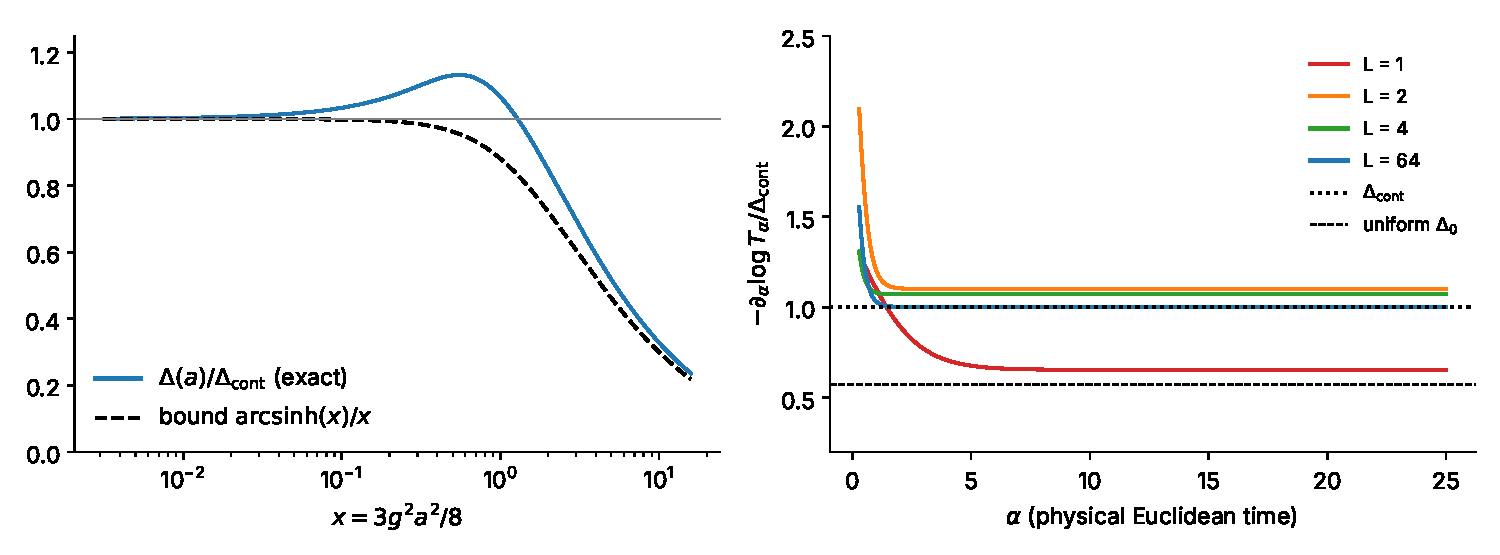
\includegraphics[width=\textwidth]{figures/op1_2d_uniform.pdf}
\caption[Left: the exact lattice gap in units of the continuum gap, against the bound]{Left: the exact lattice gap in units of the continuum gap, against the bound $\operatorname{arcsinh}(x)/x$ of Theorem~\ref{thm:2dB}. The exact ratio overshoots $1$, with a maximum of about $1.13$ near $x\approx0.55$, so the approach to the continuum is not monotone, while the bound is. Right: Thorin local rates in physical units for $L=1,2,4,64$ at $\ell=3$ and $g=1$, all above the uniform $\Delta_0$, the curves for large $L$ approaching $\Delta_{\mathrm{cont}}$.}
\label{fig:2duniformB}
\end{figure}

\subsection{The anatomy of the proof}

The proof has three ingredients, and it is worth naming them because the rest of the book tries to reproduce each in four dimensions.
\begin{enumerate}
\item[(i)] Exact decimation. Coarse graining is a convolution of laws, diagonal in characters, so the transfer matrix eigenvalue is an explicit function of the coupling.
\item[(ii)] A special function inequality. The Bessel ratio bound controls the eigenvalue at every coupling, from strong to weak, and scales like $a^2$ at weak coupling, which exactly cancels the conversion to physical units.
\item[(iii)] The equivalence theorem. A uniform spectral gap is a uniform Thorin gap inequality with constant one.
\end{enumerate}
In four dimensions, ingredient (iii) is available unchanged. Ingredient (i) fails: coarse graining on $\Z^4$ is not a convolution of plaquette laws. The Migdal Kadanoff\index{Migdal Kadanoff recursion} recursion of Section~\ref{ch:mk} restores it at the price of an approximation, by combining convolution with a Bayesian product. Ingredient (ii) becomes the decrement inequality of Section~\ref{ch:verification}.

\section{A Guided Tour in Two Dimensions}\label{ch:tour}\index{two dimensions}\index{decimation}

Two dimensional SU(2) lattice gauge theory is the one case in which every object of this book can be written down and computed in a line. This section walks through the whole argument there, with numbers, as a map of the method. Nothing in it is new. The table and Figure~\ref{fig:tour2d} are exact and are produced by \texttt{code/tour2d.py}; the only Monte Carlo numbers are the ones quoted under Computation, which are checked against exact answers.

\subsection{The measure and its plaquette law}

In two dimensions on the plane, after gauge fixing on a tree, the plaquette variables are independent, each with the Wilson law $e^{\beta\cos\theta}$ times the Haar density $\frac2\pi\sin^2\theta$ on the rotation angle. The normalised character coefficients are ratios of Bessel functions, $u_n=I_n(\beta)/I_1(\beta)$, and the mean plaquette is $u_2$.

\begin{center}
\small
\begin{tabular}{cccccc}
\toprule
$\beta$ & $u_2$ & $u_3$ & $-\log u_2$ & gap ratio & bound \\ \midrule
0.5 & 0.124 & 0.010 & 2.090 & 0.697 & 0.606 \\
1 & 0.240 & 0.039 & 1.426 & 0.951 & 0.797 \\
2 & 0.433 & 0.134 & 0.837 & 1.116 & 0.924 \\
4 & 0.658 & 0.342 & 0.418 & 1.116 & 0.978 \\
8 & 0.819 & 0.590 & 0.199 & 1.063 & 0.994 \\
16 & 0.908 & 0.773 & 0.097 & 1.032 & 0.999 \\
32 & 0.954 & 0.881 & 0.048 & 1.016 & 1.000 \\
\bottomrule
\end{tabular}
\end{center}

\begin{figure}[t]
\centering
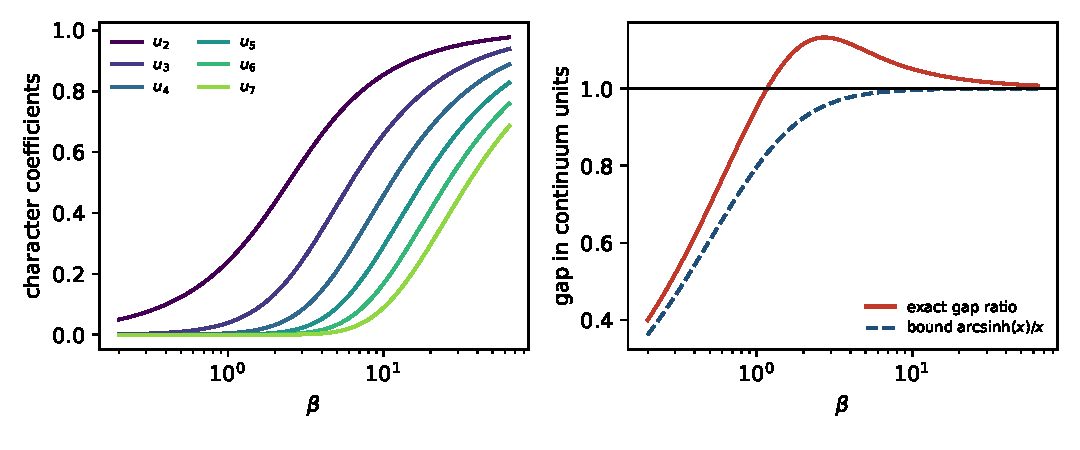
\includegraphics[width=\textwidth]{figures/tour2d.pdf}
\caption[Two dimensional SU(2) at a glance]{Left: the character coefficients $u_n=I_n(\beta)/I_1(\beta)$ of the Wilson plaquette law, $n=2,\dots,7$. Right: the exact lattice gap in units of the continuum gap, and the lower bound from Amos's inequality.}
\label{fig:tour2d}
\end{figure}

Figure~\ref{fig:tour2d} shows the coefficients and the gap across four decades of coupling.

\subsection{Positivity and the spectral measure}

The transfer matrix acts on class functions and is diagonal in the characters, with eigenvalues proportional to $u_n$. Reflection positivity is the statement that these eigenvalues are positive, which is the positivity of the Bessel functions. The spectral measure of a class function observable is a sum of point masses at the energies $E_n=-\log u_n$ in lattice units, and the gap is $E_2=-\log u_2$, the fourth column of the table. The same number is the string tension in lattice units: in two dimensions the Wilson loop of area $A$ is exactly $u_2^A$.

\subsection{The two routes}

Route A: the correlation $\sum_nc_ne^{-E_n\tau}$ with $c_n\ge0$ is the Laplace transform of a positive measure with atoms at the $E_n$; after an offset it is the Thorin measure of a convolution of gamma variables, and the gap is the smallest rate. Route B: the $2\sin^2$ lemma turns the same measure into the Thorin density $T_\alpha(z)=\sum_nc_ne^{-\alpha E_n}\,2\sin^2(E_ny/2)/(\pi y)$ with $y=\sqrt{2z}$, a sum of positive oscillations whose amplitudes decay in $\alpha$ at the rates $E_n$. The slowest is $E_2$.

\subsection{The uniform bound}

The fifth column is the lattice gap in units of the continuum gap, $(-\log u_2)/x$ with $x=3/(2\beta)$, and the sixth is the bound $\operatorname{arcsinh}(x)/x$ of Theorem~\ref{thm:2dB}, which follows from Amos's inequality for Bessel ratios. The bound holds in every row. The gap ratio overshoots one at intermediate coupling and returns to it from above in the continuum limit. A uniform Thorin gap inequality therefore holds from the coarsest lattice to the continuum, which is the conjecture of Section~\ref{ch:isthere} in a case where it is a theorem.

\subsection{Renormalization}

Decimation by a scale factor $b$ is exact in two dimensions (Section~\ref{sec:su2bm}): character coefficients are raised to the power $b^2$, $u_n\mapsto u_n^{b^2}$. In two dimensions bond moving has power $b^{d-2}=1$ and does nothing, so the Migdal Kadanoff ladder is the exact renormalization group, and the two caricatures of Chapter~\ref{ch:sandwich} both coincide with the truth. The width of the bracket in $d$ dimensions is governed by the bond moving power $b^{d-2}$: one in two dimensions, $b$ in three, $b^2$ in four. In the ladder, dimension enters through that exponent alone.

In the heat kernel family, $u_n=e^{-(n^2-1)t/4}$, decimation is $t\mapsto b^2t$: the coupling $\beta=2/t$ is divided by $b^2$ at every step. The coupling is relevant, the flow reaches strong coupling after $\frac12\log_b\beta$ steps, and the gap in physical units is constant along the flow. There is no asymptotic freedom to prove and no crossover to control.

\subsection{Approach to Haar measure}

By the Fourier bound of Section~\ref{ch:h6}, the law of a block of $m$ plaquettes is within $\frac12\big(\sum_{n\ge2}n^2u_n^{2m}\big)^{1/2}$ of Haar measure in total variation. With $m=4$ this is $0.003$ at $\beta=1$, $0.035$ at $\beta=2$ and $0.19$ at $\beta=4$. Confinement in two dimensions is Poincar\'e's shuffle: enough independent group elements multiplied together are uniformly distributed.

\subsection{Computation}

The Monte Carlo estimators of Chapters~\ref{ch:estimation} and~\ref{ch:kac} reported below were tested here against exact answers. On a $3\times3$ torus, $\log Z(2)=-13.8223$ from the character formula; over three seeds the root mean square errors are $0.032$ for the vertical likelihood family, $0.057$ for path sampling (the power posterior), $0.117$ for prior importance sampling, $0.140$ for split sampling, $0.218$ for nested sampling and $0.275$ for the harmonic mean estimator, whose error changes sign across seeds. Pseudolikelihood recovers $\beta$ from one configuration of a $12\times12$ torus to about $15$ percent at $\beta\le2$ and about $5$ percent at $\beta\ge4$. The heat bath is a slice sampler on the three sphere, and Conjecture~\ref{prop:slicecurv}, whose proof is only sketched (the smoothing of the corners of the slice is not carried out), would give its sliced conditional a log Sobolev constant of two, under the positivity hypothesis of that conjecture on every slice level.

\subsection{What two dimensions does not teach}

Three things are absent. There is no bond moving, so no nonlinearity in the renormalization map and no need for the likelihood ratio order. There is no marginal coupling, so no first passage time and no exponentially small scale. And there are no glueballs: the spectrum is that of a single quantum mechanical particle on the group, not of a field theory with propagating degrees of freedom. The rest of the book is about putting those three things back.

\section{Riemann's Kernel and the Three Sphere}\label{ch:riemann}

This section records an identity that connects the two problems of our research programme. Riemann's kernel $\Phi$, whose Fourier transform is the function $\Xi$ of the Riemann Hypothesis\index{Riemann Hypothesis}, is built from the return density of Brownian motion\index{Brownian motion on SU(2)} on SU(2), which is also the partition function of two dimensional Yang Mills theory on the sphere.

\subsection{Riemann's kernel}

Riemann's 1859 memoir~\cite{Ri59} writes the completed zeta function, evaluated on the critical line, as a cosine transform. With
\[
\Phi(u)=\sum_{n\ge1}\big(2\pi^2n^4e^{9u/2}-3\pi n^2e^{5u/2}\big)\exp\big(-\pi n^2e^{2u}\big),
\]
one has
\[
\Xi(x)=4\int_0^\infty\Phi(u)\cos(xu)\,\mathrm du,
\]
where $\Xi(x)=\xi(\tfrac12+ix)$. The kernel $\Phi$ is positive, even, and decays like a double exponential. P\'olya~\cite{Po26} studied the zeros of transforms of this kind; de Bruijn~\cite{dB50} and Newman~\cite{Ne76} studied the deformation $\int e^{\lambda u^2}\Phi(u)\cos(xu)\mathrm du$, which is a backward heat flow on $\Xi$; and the Riemann Hypothesis is the statement that all zeros of $\Xi$ are real. In our Riemann programme $\Phi$, normalised, is the starting point of the probabilistic constructions.

\subsection{The return density of Brownian motion on SU(2)}

The density of Brownian motion on SU(2) at the identity is the heat kernel\index{heat kernel} at $\theta=0$. Since $\chi_n(0)=n$,
\[
K_t(e)=\sum_{n\ge1}n^2e^{-t(n^2-1)/4}.
\]
The partition function of two dimensional SU(2) Yang Mills theory on the sphere is $Z_0(A)=\sum_nn^2e^{-A(n^2-1)/8}$, so
\[
Z_0(A)=K_{A/2}(e):
\]
the sphere partition function at area $A$ is the probability density that Brownian motion on the three sphere, run for time $A/2$, returns to its starting point. This is the probabilistic content of Witten's observation that the sphere partition function is a heat kernel evaluated at the identity.

\subsection{The identity}

\begin{proposition}\label{prop:riemannB}
Let $F(A)=\sum_{n\ge1}n^2e^{-An^2/8}=e^{-A/8}Z_0(A)$. With $A=8\pi e^{2u}$,
\[
\Phi(u)=-16\pi^2e^{9u/2}F'(A)-3\pi e^{5u/2}F(A).
\]
\end{proposition}

\begin{proof}
At $A=8\pi e^{2u}$ we have $e^{-An^2/8}=e^{-\pi n^2e^{2u}}$, and differentiating gives $\sum_nn^4e^{-An^2/8}=-8F'(A)$. Substituting into the definition of $\Phi$ gives the formula.
\end{proof}

So Riemann's kernel is a linear combination, with coefficients depending on $u$, of the return density of Brownian motion on the three sphere and its time derivative, evaluated at time $t=A/2=4\pi e^{2u}$. The derivative has a physical meaning of its own: $-\partial_A\log Z_0$ is the expected action per unit area in two dimensional Yang Mills on the sphere. We checked the identity numerically to fifteen digits (Figure~\ref{fig:riemannB}).

\begin{figure}[t]
\centering
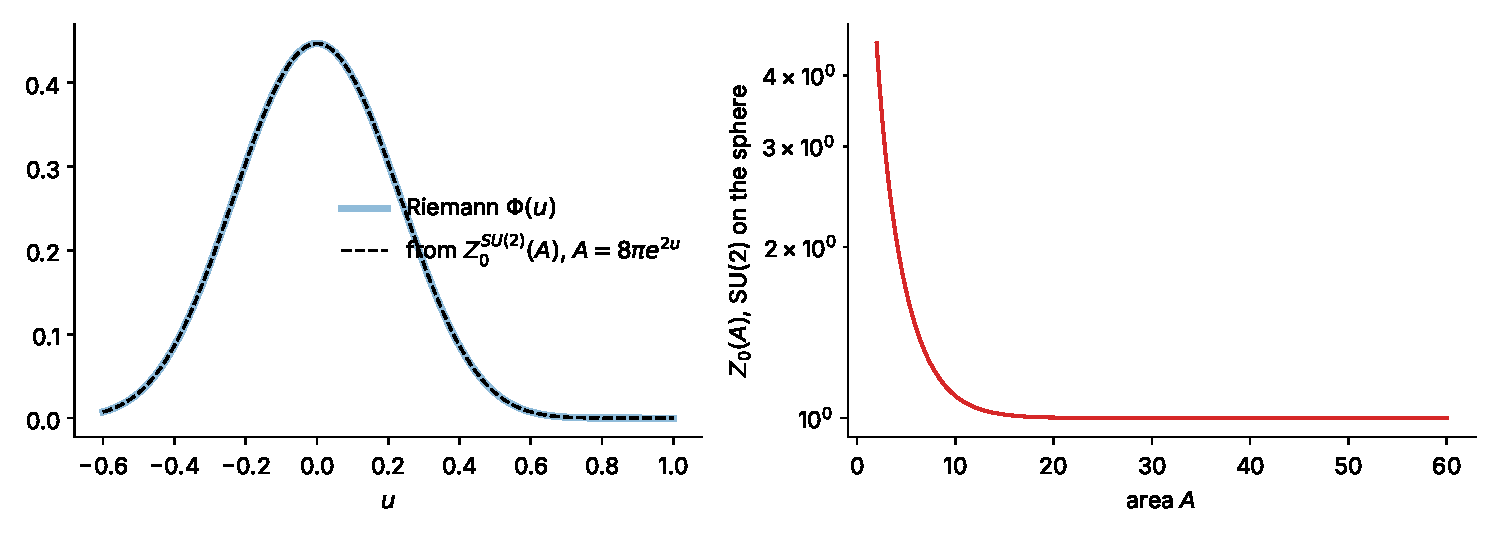
\includegraphics[width=\textwidth]{figures/riemann_kernel_ym.pdf}
\caption[Left: Riemann's $\Phi(u)$ and the same function built from the SU(2) sphere partition function at]{Left: Riemann's $\Phi(u)$ and the same function built from the SU(2) sphere partition function at $A=8\pi e^{2u}$. Right: the sphere partition function $Z_0(A)$, the return density of Brownian motion on $S^3$ at time $A/2$.}
\label{fig:riemannB}
\end{figure}

\subsection{The functional equation as an area duality}

Riemann's functional equation $\xi(s)=\xi(1-s)$ is equivalent to the evenness $\Phi(u)=\Phi(-u)$. Under the identity, $u\mapsto-u$ sends $A=8\pi e^{2u}$ to $8\pi e^{-2u}=64\pi^2/A$. The functional equation therefore becomes a relation between the sphere theory at area $A$ and at area $64\pi^2/A$. On the Yang Mills side this is the Poisson resummation that turns the sum over representations into a sum over classical solutions, the instanton expansion of two dimensional Yang Mills. On the Brownian side it is the relation between the spectral sum and the image sum of Section~\ref{sec:su2bm}: small times on one side correspond to large times on the other.

\subsection{The Biane, Pitman and Yor connection}

The same theta sums appear in the work of Biane, Pitman and Yor~\cite{BPY} on laws tied to Brownian excursions and Bessel bridges. They show that $\xi$ is, up to normalisation, the Mellin transform of a probability law built from these sums, and that the hyperbolic laws $C$, $S_{\mathrm{BPY}}$ and $T$ of Section~\ref{ch:toolkit} are the natural Laplace transform companions. Proposition~\ref{prop:riemannB} adds a gauge theoretic face to that picture: the Mellin side lives on the real line of $\log$ area, the Laplace side lives on Brownian time on SU(2), and the same function is the partition function of a gauge theory.

The variable $S_{\mathrm{BPY}}$, whose Laplace transform is $\sqrt{2q}/\sinh\sqrt{2q}$, will reappear in Section~\ref{ch:mk} for a different reason: that Laplace transform is the curvature factor $\theta/\sin\theta$ at the imaginary angle $\theta=i\sqrt{2q}$, and the mean of $S_{\mathrm{BPY}}$ controls asymptotic freedom\index{asymptotic freedom} in the Migdal Kadanoff ladder. The three sphere thus ties together Riemann's kernel, two dimensional Yang Mills, and the running of the coupling in the ladder.

\subsection{Questions}

\begin{problem}\label{op:exact1}
Study the zeros of $Z_0(A)$ in the complex area plane, the Fisher zeros of the sphere theory, and relate them through Proposition~\ref{prop:riemannB} to the zeros of $\Xi$.
\end{problem}

\begin{problem}\label{op:exact2}
The large $N$ limit of two dimensional Yang Mills on the sphere has a third order phase transition at a critical area, discovered by Douglas and Kazakov\index{Douglas, M. R.!and Kazakov, V. A.}~\cite{DK}. Track the Route B Thorin densities across the transition, and ask whether the analogue of Proposition~\ref{prop:riemannB} for SU(N) at large $N$ has a number theoretic interpretation.
\end{problem}

Neither problem bears directly on the four dimensional mass gap\index{mass gap}. We include them because they show that the probabilistic objects of this book are not chosen arbitrarily: the same laws on the same group appear on both sides of our programme.

\section{Dynamic and Static Gaps}\label{ch:dynamic}\index{log Sobolev inequality}\index{spectral gap!dynamic}\index{Bakry \'Emery criterion}\index{Shen, H.!Zhu, R. and Zhu, X.}

The mass gap is a static property of a measure: correlations decay exponentially. A Markov chain that samples the measure has its own spectral gap, a dynamic property. This section explains how the two are related, for which models they are known to be equivalent, why that equivalence suggests a second route to the mass gap, and how far that route has been taken for lattice Yang Mills.

\subsection{Two gaps for one measure}

Let $\mu$ be a Gibbs measure on a lattice and $\mathcal L$ the generator of a reversible local dynamics, such as heat bath Glauber dynamics, with $\mu$ as invariant measure. The spectral gap of the dynamics is
\[
\mathrm{gap}(\mathcal L)=\inf_f\frac{\mathcal E(f,f)}{\operatorname{Var}_\mu f},
\]
the smallest nonzero eigenvalue of $-\mathcal L$, where $\mathcal E$ is the Dirichlet form. The logarithmic Sobolev constant is defined similarly with entropy in place of variance. The static gap is the mass gap of the transfer matrix, the decay rate of spatial correlations.

For the Ising chain both can be computed. The static gap is $-\log\tanh\beta$. The dynamic gap of heat bath dynamics on a ring of ten sites can be found by diagonalising its $1024\times1024$ generator. Figure~\ref{fig:dynstat} shows both: they decrease together as $\beta$ grows and the correlation length increases. They are not equal, one being a rate per unit time and the other per unit length, but for the chain both tend to zero as $\beta\to\infty$. In general the static gap defined here, exponential decay of correlations in one state (weak mixing), is weaker than the strong spatial mixing of the next paragraph.

\begin{figure}[t]
\centering
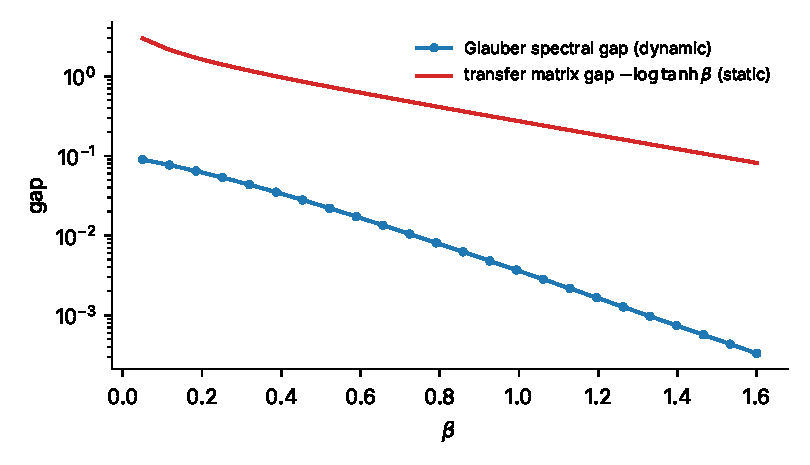
\includegraphics[width=0.85\textwidth]{figures/dynamic_static_gap.pdf}
\caption[Dynamic and static gaps for the Ising chain]{Spectral gap of heat bath Glauber dynamics on a ten site Ising ring, computed exactly, and the transfer matrix gap $-\log\tanh\beta$. Both shrink as the correlation length grows.}
\label{fig:dynstat}
\end{figure}

\subsection{The equivalence theorems}

For finite range spin systems with a finite (discrete) single spin space the following are equivalent, under mild conditions on the boundary behaviour. This is the setting of the theorems quoted below. Lattice Yang Mills has compact continuous spins and a gauge symmetry, so these equivalences are not established for it in this form, and here they serve as a guide.
\begin{enumerate}
\item[(a)] Strong spatial mixing: the influence of a boundary condition decays exponentially with distance, uniformly in the volume and the boundary.
\item[(b)] The Glauber dynamics has a spectral gap bounded below uniformly in the volume.
\item[(c)] The Glauber dynamics has a logarithmic Sobolev constant bounded below uniformly in the volume.
\end{enumerate}
Dobrushin and Shlosman~\cite{DS85,DS87} introduced complete analyticity conditions that imply (a). Stroock and Zegarlinski~\cite{SZ92} proved that (c) is equivalent to Dobrushin and Shlosman complete analyticity, which is slightly stronger than (a) as stated, and Martinelli and Olivieri~\cite{MO94} extended the equivalences to the weaker regime of strong mixing for regular volumes.

\subsection{Curvature and log Sobolev}

The Bakry \'Emery criterion~\cite{BE} gives a direct way to prove (c). If the measure has density $e^{-V}$ on a Riemannian manifold with $\mathrm{Ric}+\nabla^2V\ge\kappa>0$, then it satisfies a logarithmic Sobolev inequality with constant $\kappa$. For lattice gauge theory the manifold is a product of copies of the group, whose Ricci curvature is positive, and $V=\beta S$. At small $\beta$ the Hessian of $\beta S$ is a small perturbation of the positive group curvature, and the criterion applies uniformly in the volume.

This is the route of Shen, Zhu and Zhu~\cite{SZZ}. They studied the Langevin dynamics of lattice Yang Mills at strong coupling in any dimension, proved Poincar\'e and log Sobolev inequalities uniformly in the volume when $\beta$ is below an explicit threshold, and deduced exponential ergodicity, factorisation of Wilson loop correlations at large $N$, and a positive mass gap for the infinite volume measure. Their threshold, of order $1/(16(d-1))$ for SU(N) in their scaling, is a strong coupling condition, in the same regime as the Osterwalder and Seiler cluster expansion~\cite{OSe}, but the proof is entirely through dynamics and curvature.

\subsection{A dynamic route along the ladder}

At weak coupling the Hessian of $\beta S$ is large and indefinite on the scale of the group, and the Bakry \'Emery criterion fails, as it must: the correlation length in lattice units diverges and no dynamic gap uniform in the coupling can exist on the original lattice (at fixed coupling a gap uniform in the volume is expected). The renormalization group suggests a fix. Along the Migdal Kadanoff ladder, every rung is a lattice theory at an effective coupling that decreases by about $\frac34\E S_{\mathrm{BPY}}=\frac14$ per step at leading order (Remark~\ref{prop:decrementB}), until the coupling is below the strong coupling threshold. On that final rung the Shen, Zhu and Zhu argument gives a uniform log Sobolev inequality and hence a gap, provided it applies to the non Wilson plaquette law of that rung, which has not been checked here (their argument is for the Wilson action). The gap of the original theory in physical units then follows if the comparison between rungs preserves log Sobolev constants up to the rescaling of lengths.

That is a dynamic version of the Thorin sandwich of Chapter~\ref{ch:sandwich}: instead of bracketing spectral measures, bracket Dirichlet forms. Comparisons of Dirichlet forms are a standard tool in Markov chain theory, but whether they behave well under the two operations of the ladder is open. The bond moving step multiplies densities on the same group ($f\mapsto f^4$), so it does not produce a product measure on a product space and tensorisation of log Sobolev constants does not apply to it; under such pointwise reweighting the constants are controlled only by perturbation bounds that degrade with the oscillation of $\log f^4$. For convolution with a heat kernel the control by Bakry \'Emery calculus on the group has not been worked out here. The open question is the same as before, the comparison between the ladder and the true lattice, but in a language where more tools are available.

\section{The Renormalization Group for Statisticians}\label{ch:rg}\index{renormalization group}\index{hierarchical lattice}\index{Gaussian ledger}

The renormalization group is the central idea of modern statistical physics, and it is close in spirit to ideas statisticians use every day: hierarchical models, sufficient reductions, and the propagation of uncertainty through levels. This section explains it in that language, with the Migdal Kadanoff ladder as the running example.

\subsection{Coarse graining as marginalisation}

Start with a probability model for fine scale variables, the spins or links of a lattice. Group them into blocks and define a block variable for each, such as a majority vote or an average. The law of the block variables is a marginal of the original law. If it has the same form as the original, with changed parameters, we have a map on parameters, the renormalization map. Iterating it describes the model at larger and larger scales.

In Bayesian terms, the fine variables are latent, the block variables are a coarse summary, and the renormalization map is the update of the hyperparameters that describe the summary. The question the renormalization group asks is what happens to those hyperparameters after many levels. Most hyperparameters become irrelevant: their influence on the coarse law decays. A few are relevant or marginal and determine the large scale behaviour.

\subsection{Fixed points and flows}

A fixed point of the renormalization map is a model that looks the same at every scale. Near a fixed point the map is approximately linear, and its eigenvalues classify directions as relevant, growing under the flow; irrelevant, shrinking; or marginal, neither at linear order. Critical points of statistical models sit on the stable manifolds of nontrivial fixed points, and the exponents of correlation functions are read off from the eigenvalues.

For Yang Mills the relevant picture has two fixed points: the free theory at $g=0$, which is the ultraviolet fixed point, and a strong coupling, confining regime that acts as an infrared attractor. The coupling is marginal at the free fixed point, and its slow logarithmic flow away from it is asymptotic freedom. The continuum limit is the renormalized trajectory that leaves the free fixed point, and the mass gap is the statement that this trajectory ends in the confining regime with a finite correlation length in physical units.

\subsection{Exact renormalization: chains and hierarchical models}

The Ising chain has an exact renormalization map, $\tanh K'=(\tanh K)^2$, from Section~\ref{ch:examples}. Every coupling flows to zero, the disordered fixed point, and the correlation length halves at each step. Two dimensional lattice gauge theory has the same structure, with character coefficients raised to the power $b^2$.

Dyson~\cite{Dy69} introduced hierarchical models, in which the interaction between two spins depends on the level of the smallest block containing both. Their renormalization map is exact by construction, and Bleher and Sinai~\cite{BS73} used them to study critical behaviour rigorously. Migdal Kadanoff lattices, built by repeatedly replacing a bond by a diamond of bonds, are hierarchical lattices on which the Migdal Kadanoff recursion is exact. For spin models that is the diamond construction; a gauge theory needs a plaquette complex, and the gauge version is the one of~\cite{Ito85}. If the gauge recursion of Sections~\ref{ch:mk} and~\ref{ch:verification} is accepted as the exact renormalization of that model, as taken from~\cite{Ito85} and not reproved here, then the ladder is a statement about a real statistical model, the gauge theory on a hierarchical lattice, as well as an approximation to the theory on $\Z^4$.

\subsection{The Gaussian ledger, again}

For Gaussian models the renormalization map is linear algebra. The ledger of Section~\ref{ch:mk}, precisions add under products and variances add under convolutions, makes the four dimensional coupling exactly marginal in flat space. Figure~\ref{fig:ledger} illustrates the consequence, schematically: in flat space the coupling stays where it starts; on the curved group it decreases by a fixed amount per step until strong coupling takes over and it collapses.

\begin{figure}[t]
\centering
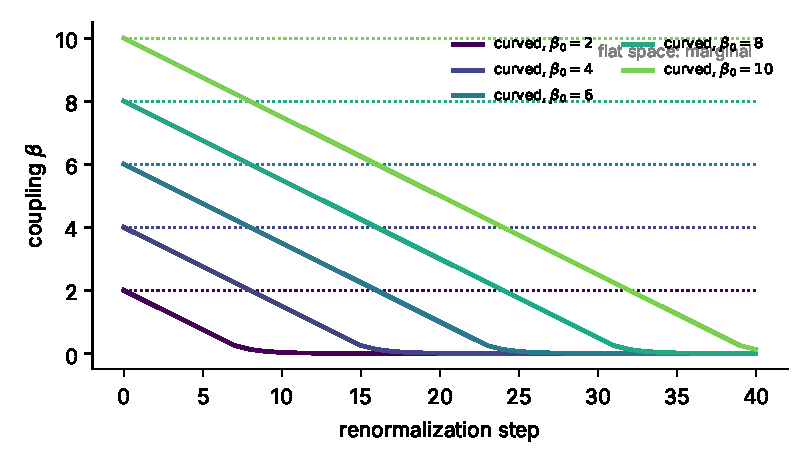
\includegraphics[width=0.85\textwidth]{figures/gaussian_ledger.pdf}
\caption[The Gaussian ledger in flat and curved space]{Schematic renormalization flow of the coupling. Dotted: flat space, where the four dimensional coupling is marginal. Solid: the curved group, where each step lowers the coupling by about $1/4$ until the strong coupling region is reached.}
\label{fig:ledger}
\end{figure}

\subsection{The flow in the space of plaquette laws}

The Migdal Kadanoff map acts on whole plaquette laws, not just one coupling. Figure~\ref{fig:mkphase} projects the flow onto the first two Thorin levels $(u_2,u_3)$. Numerically, trajectories started at weak and intermediate coupling ($\beta_0=3,5,8,12$) lock onto a single curve toward the origin, the heat kernel family $u_3=u_2^{8/3}$. This is a numerical observation, not a theorem, and it is restricted to weak and intermediate coupling: near the origin every trajectory leaves the curve (at strong coupling the character expansion gives $u_3\sim c\,u_2^2$, not $u_2^{8/3}$), and a trajectory started at $\beta_0=0.8$ never reaches it. On linear axes the departure is invisible because $u_3$ is tiny. So the heat kernel laws attract the flow only in that range, and that is the only statistical justification offered for the one dimensional projection used in Section~\ref{ch:verification}.

\begin{figure}[t]
\centering
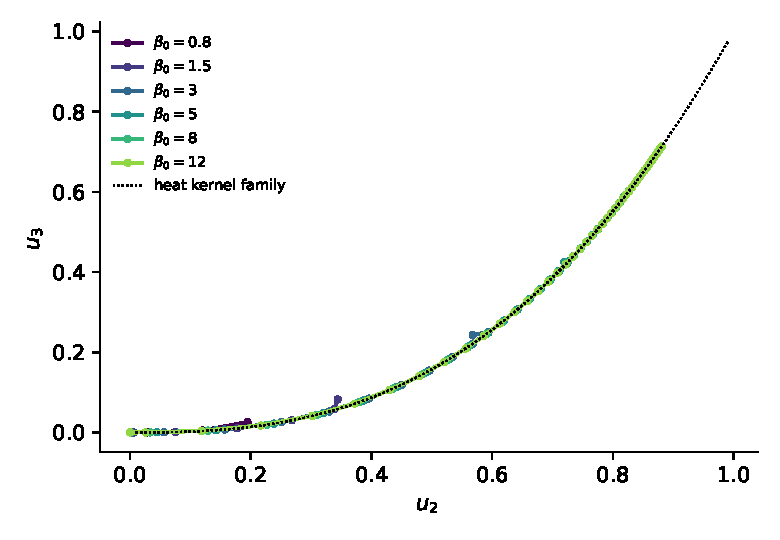
\includegraphics[width=0.85\textwidth]{figures/mk_phase.pdf}
\caption[The Migdal Kadanoff flow in the plane of Thorin levels]{Migdal Kadanoff trajectories for SU(2) projected onto $(u_2,u_3)$, from several Wilson starting couplings. Started at weak and intermediate coupling they follow the heat kernel family $u_3=u_2^{8/3}$, shown dotted (numerical observation); near the origin they leave it.}
\label{fig:mkphase}
\end{figure}

\subsection{Renormalization and hierarchical Bayes}

The analogy with hierarchical Bayesian models runs deep. A hierarchical model with many levels, each level a convolution of the one below with a prior and a product with the data at that level, is a renormalization group in reverse: information flows from coarse to fine. Shrinkage priors such as the horseshoe have a scale mixture structure in which the local scales play the role of irrelevant variables and the global scale the role of a marginal coupling, and the behaviour of the global scale across levels is the statistical analogue of the running coupling. Polson and Scott's duality between envelopes and mixtures~\cite{PSdual} is the bookkeeping of products and convolutions that the Migdal Kadanoff step uses.

\section{Free Fields and Exact Spectral Measures}\label{ch:freefield}\index{free field}\index{K\"all\'en Lehmann representation}

Before an interacting theory, a free one. A free massive field has a gap equal to its mass, and every spectral measure of its local observables is explicit. This section computes them, shows how Routes A and B look when everything is known, and explains which features of the free field survive in Yang Mills and which do not.

\subsection{The K\"all\'en Lehmann representation}

For a free scalar field of mass $m$ in $d$ spacetime dimensions, the zero momentum correlation of the field itself is a single exponential, $C(\tau)\propto e^{-m\tau}$, with spectral measure a point mass at $m$. Composite operators have continuous spectra. The operator $\phi^2$ at zero spatial momentum creates pairs of particles with momenta $p$ and $-p$, of total energy $E=2\sqrt{m^2+p^2}$. Counting states in $d-1$ spatial dimensions and including the normalisation $1/(2\omega)^2$ of each pair gives the spectral density
\[
\rho(E)\propto\frac{(E^2/4-m^2)^{(d-3)/2}}{E},\qquad E>2m .
\]
In two dimensions the density has an inverse square root singularity at threshold; in three it jumps to a constant times $1/E$; in four it rises from zero like a square root (Figure~\ref{fig:ff}). In all cases the support starts at $2m$, so the gap of $\phi^2$ is $2m$, twice the gap of $\phi$. The gap of the theory is the infimum over observables, $m$.

\begin{figure}[t]
\centering
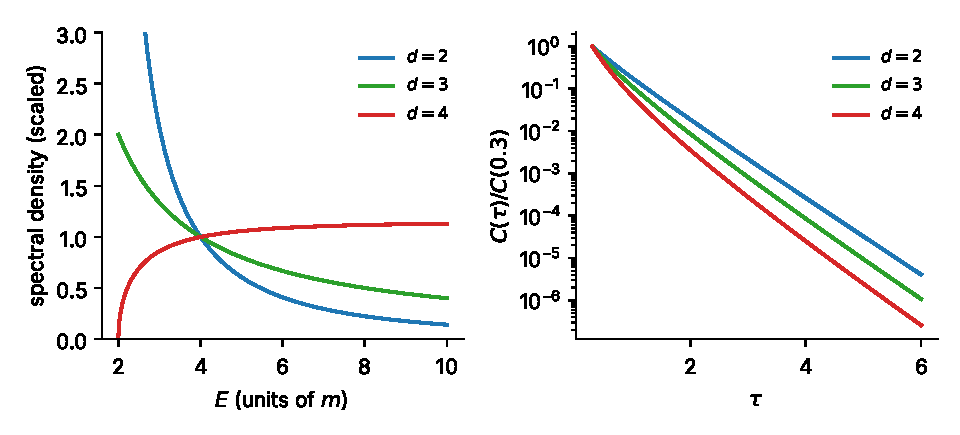
\includegraphics[width=\textwidth]{figures/free_field_kl.pdf}
\caption[Spectral densities of $\phi^2$ for a free field]{Left: zero momentum spectral densities of $\phi^2$ for a free field of mass one in $d=2,3,4$. Right: the corresponding Euclidean correlations, normalised at $\tau=0.3$; all decay at rate $2m=2$, with a power law prefactor set by the threshold behaviour.}
\label{fig:ff}
\end{figure}

\subsection{Routes A and B for a free field}

For the elementary field, Route A gives a gamma variable with rate $m$, and Route B a single damped oscillation in real time. For $\phi^2$, Route A gives a GGC with a continuous Thorin density supported on $[2m,\infty)$, and its tail is expected to be $e^{-2mx}$ times a power determined by the threshold exponent $(d-3)/2$ (a Tauberian computation left to the exercises and not carried out here). Route B gives Thorin densities $T_\alpha(z)$ whose decay rate in $\alpha$ is $2m$ and whose dependence on real time reflects the shape of the density at threshold.

Figure~\ref{fig:thorinheat} shows a Route B Thorin density as a colour map in Euclidean and real time, for the toy glueball spectrum of earlier chapters. The density decays along the Euclidean axis at the gap and oscillates along the real time axis at the frequencies of the stable states, with the continuum smoothing the oscillations at large real time.

\begin{figure}[t]
\centering
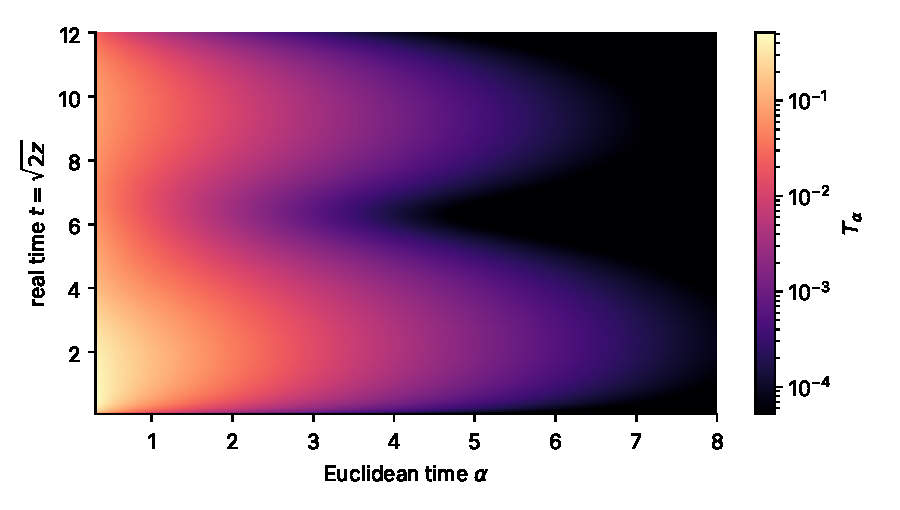
\includegraphics[width=\textwidth]{figures/thorin_heatmap.pdf}
\caption[A Route B Thorin density as a colour map]{The Route B Thorin density $T_\alpha$ for the toy glueball spectrum, as a function of Euclidean time $\alpha$ and real time $y=\sqrt{2z}$, on a logarithmic colour scale. Decay along $\alpha$ is set by the gap; oscillation along $y$ by the stable states.}
\label{fig:thorinheat}
\end{figure}

\subsection{What survives in Yang Mills}

Three features of the free field carry over. The gap of the theory is the infimum over observables, and composite observables have continuous spectra above multiparticle thresholds. Ultraviolet divergences of composite operators, visible here as the failure of $\rho(E)$ to decay at large $E$ in four dimensions, require the offset of Chapter~\ref{ch:positivity}. And the Thorin structure is the same: positive spectral measures, Routes A and B, the equivalence theorem.

Two features do not survive. In Yang Mills there is no elementary field whose spectral measure is a single atom: gauge invariant observables are composite, and the lightest state is expected, on lattice evidence, to be a bound state, the scalar glueball (its mass is a lattice Monte Carlo estimate~\cite{Te98,MP}, not an established fact), whose mass is not a parameter of the Lagrangian but is generated dynamically as a multiple of $\Lambda$. And the free field has a gap because its mass is put in by hand. The entire difficulty of the Clay problem is that Yang Mills has no mass term, and the gap must be produced by the renormalization group flow from the massless free fixed point. A free massive field is the answer we expect the long distance limit to resemble, not a step on the way to proving it.

\section{Large N and Free Probability}\label{ch:largeN}\index{large $N$}\index{Gross Witten Wadia transition}\index{free probability}

't Hooft~\cite{tH74} observed in 1974 that SU(N) gauge theory simplifies as $N\to\infty$ with $\lambda=g^2N$ fixed: only planar diagrams survive, and the theory becomes a theory of strings. Large $N$ is where gauge theory meets random matrix theory and free probability, both close to the probabilistic toolkit of this book. This section explains what large $N$ says about the gap.

\subsection{The Gross Witten Wadia transition}

The simplest large $N$ lattice gauge theory is a single plaquette, or equivalently two dimensional lattice gauge theory, with weight $\exp(\frac N\lambda\operatorname{tr}(U+U^\dagger))$ on a single unitary matrix. Gross and Witten~\cite{GW80}, and independently Wadia, solved it at large $N$. The eigenvalue angles $\theta\in(-\pi,\pi]$ of $U$ have a limiting density that changes form at $\lambda=2$:
\[
\rho(\theta)=\begin{cases}\dfrac{2}{\pi\lambda}\cos\dfrac\theta2\sqrt{\dfrac\lambda2-\sin^2\dfrac\theta2}, & \lambda<2,\\[1.2em] \dfrac{1}{2\pi}\Big(1+\dfrac2\lambda\cos\theta\Big), & \lambda\ge2 .\end{cases}
\]
At weak coupling the eigenvalues are confined to an arc and the density has a gap on the circle; at strong coupling they cover the whole circle (Figure~\ref{fig:gww}). The free energy is analytic on each side but its third derivative jumps at $\lambda=2$: a third order phase transition, which exists only at infinite $N$.

\begin{figure}[t]
\centering
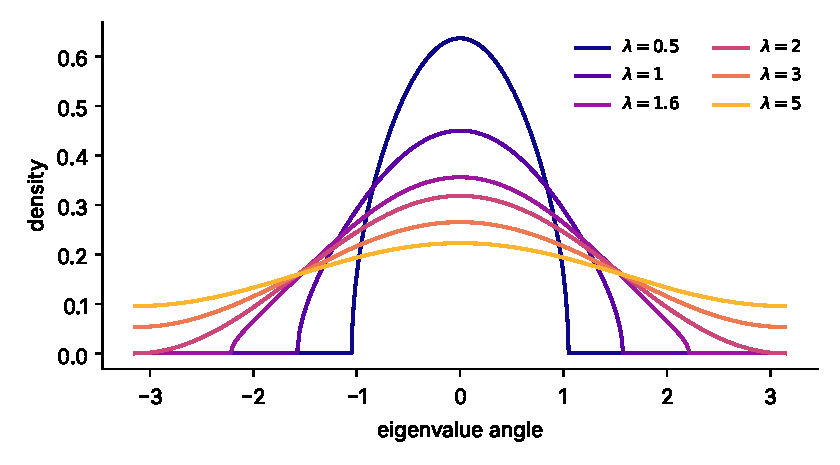
\includegraphics[width=0.85\textwidth]{figures/gww.pdf}
\caption[Gross Witten Wadia eigenvalue densities]{Limiting eigenvalue densities of the Gross Witten Wadia model for several values of $\lambda$. Below $\lambda=2$ the support is an arc; above, the whole circle.}
\label{fig:gww}
\end{figure}

Douglas and Kazakov~\cite{DK} found the analogous transition in continuum two dimensional Yang Mills on the sphere, at a critical area. In both cases the transition separates a weak coupling phase, dominated by small fluctuations around the identity, from a strong coupling phase, dominated by disordered eigenvalues.

\subsection{Free Brownian motion on the unitary group}

As $N\to\infty$, Brownian motion on U(N) has a limit in the sense of free probability: the eigenvalue distribution at time $t$ converges to a deterministic law on the circle, the law of Biane's free unitary Brownian motion~\cite{Bi97}. For small $t$ the support is an arc that grows with $t$; at $t=4$ it closes up and covers the circle. Two dimensional Yang Mills at large $N$ is governed by this process, the master field (Levy~\cite{Le17} constructed the master field on the plane as the large $N$ limit of planar Yang Mills holonomies, which satisfies the Makeenko Migdal equations), and the Douglas Kazakov transition is where the free unitary Brownian motion bridge from the identity back to itself can no longer avoid wrapping around the circle.

The three sphere heat kernel of Section~\ref{sec:su2bm}, shown as a colour map in Figure~\ref{fig:hkheat}, is the $N=2$ case of Brownian motion on SU($N$), although Biane's time normalisation differs from the one used for $K_t$. As $N$ grows, the heat kernel on SU(N) concentrates, and its eigenvalue distribution becomes deterministic.

\begin{figure}[t]
\centering
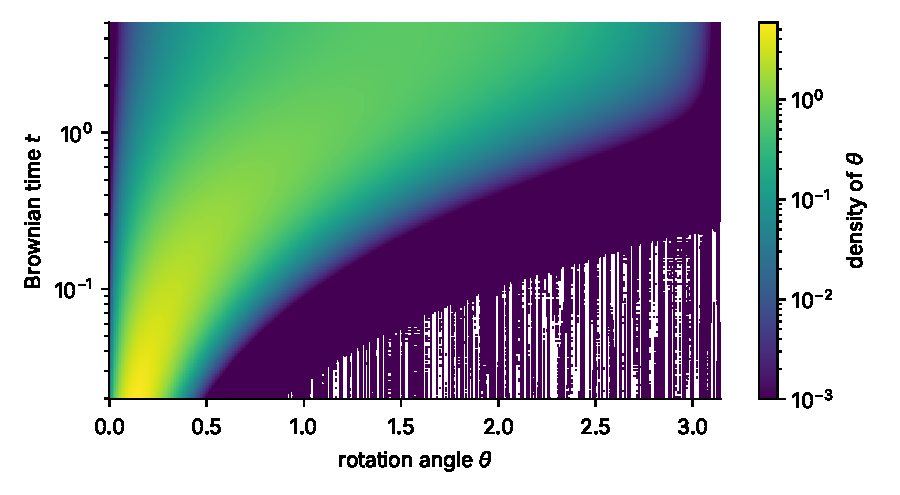
\includegraphics[width=\textwidth]{figures/heat_kernel_heatmap.pdf}
\caption[The SU(2) heat kernel as a colour map]{Density of the rotation angle of Brownian motion on SU(2) as a function of Brownian time, on a logarithmic colour scale. At small times the mass sits near the identity; by $t\approx5$ the law is close to Haar.}
\label{fig:hkheat}
\end{figure}

\subsection{What large N says about the gap}

At large $N$ the glueball masses, in units of the string tension, are expected to have finite limits, and lattice computations indicate that they are close to their $N=3$ values~\cite{Te98}. The large $N$ theory is believed to have a gap, and it is a theory of free glueballs: glueball scattering amplitudes vanish like $1/N^2$. In the language of this book, the spectral measure of a single trace observable at large $N$ is a sum of point masses, the stable glueballs, with no multiparticle continuum at leading order. Route A then gives a convolution of gamma variables, and Route B a sum of damped oscillations.

The large $N$ limit does not make the Clay problem easier in any known way. The master field is understood in two dimensions, where it is free unitary Brownian motion, but not in four. What large $N$ does supply is a family of exactly solvable caricatures in Kac's sense, where the relation between the eigenvalue distribution of the plaquette and the confining behaviour can be studied, and where free probability, a probabilistic theory, is the natural language.

\section*{Exercises}
\begin{enumerate}
\item Derive the eigenvalues $u_n(\beta)^L$ of the two dimensional transfer matrix on a cylinder of $L$ sites by integrating out the links of one time slice.
\item Using Amos's lower bound, show that $\Delta(a)\le\frac{g^2\ell\beta}{4}\operatorname{arcsinh}(2/\beta)$, and find the limit of this upper bound as $a\to0$.
\item Compute the two dimensional Yang Mills partition function on the torus for SU(2) (Section~\ref{sec:su2bm}) as a theta function and use the Jacobi transformation to find its behaviour as $A\to0$.
\item Verify the row $\beta=2$ of the table of Section~\ref{ch:tour}.
\item Show that the Wilson loop of area $A$ in two dimensions is $u_2^A$, and that the potential between static charges is linear at every coupling.
\item Show that the gap ratio $(-\log u_2)/x$ tends to one as $\beta\to\infty$ and to zero as $\beta\to0$.
\item Compute the spectral gap of heat bath dynamics for a single Ising spin in a field.
\item Show that a logarithmic Sobolev inequality implies a Poincar\'e inequality with the same constant.
\item Show that the log Sobolev constant of a product measure on a product space is the minimum of the constants of its factors, and explain why this does not apply to the bond moving step $f\mapsto f^4$ of Section~\ref{ch:dynamic}.
\item Derive the Ising chain renormalization map and its fixed points (Section~\ref{ch:rg}).
\item For a Gaussian free field on $\Z^d$, compute the renormalization of the mass term under block averaging and show it is relevant.
\item Verify that the heat kernel family is invariant under decimation and explain why it is approximately invariant under bond moving at weak coupling.
\item Derive the two particle spectral density of $\phi^2$ in $d$ dimensions.
\item Compute the Route A Thorin measure for $\phi^2$ in two dimensions and its tail.
\item Show that the zero momentum correlation of $\phi^2$ in four dimensions diverges as $\tau\to0$ and find the rate.
\item Verify that both Gross Witten Wadia densities integrate to one and agree at $\lambda=2$.
\item Compute the first moment $\int\cos\theta\,\rho(\theta)\mathrm d\theta$ on each side of the transition and show that it is continuous with a continuous derivative.
\item Explain why the third order transition cannot occur at finite $N$.
\end{enumerate}

\part{The Ladder}
\chapter{Strong Coupling and the Migdal Kadanoff Ladder}\label{ch:strong}

We now move to four dimensions. Chapter~\ref{ch:twod} ended with the models that can be solved exactly, where the heat kernel and the transfer matrix gave the gap at every coupling. In four dimensions nothing is exact. This chapter treats the end of the coupling range where everything is under control, strong coupling, and explains why control there does not reach the continuum. It then describes how glueball masses are measured by lattice Monte Carlo, introduces the Migdal Kadanoff ladder, a renormalization group that can be followed from weak to strong coupling at the price of an approximation, and records what was computed on it, with the arithmetic stated. The gap between the two ends of the coupling range is the subject of the remaining chapters.

\section{Strong Coupling and the Lattice}\label{sec:strongc}

\subsection{The character expansion}

For SU(2) with the Wilson action\index{Wilson action}\cite{Wi74}, each plaquette carries the weight $e^{\beta\cos\theta_p}$, where $\theta_p$ is the rotation angle of the plaquette holonomy. Expand it in characters:
\[
e^{\beta\cos\theta}=I_1(\beta)\cdot\frac{2}{\beta}\Big(1+\sum_{n\ge2}n\,u_n(\beta)\,\chi_n(\theta)\Big),\qquad u_n=\frac{I_n(\beta)}{I_1(\beta)} .
\]
At strong coupling, $\beta\to0$, the coefficients are small: $u_n(\beta)\sim(\beta/2)^{n-1}/n!$, and in particular $u_2\sim\beta/4$. The partition function becomes a sum over assignments of representations to plaquettes, and orthogonality of characters under the Haar integrals over links forces the nonzero assignments to form closed surfaces. Each surface of $|P|$ plaquettes in the fundamental representation contributes a factor of order $u_2^{|P|}$.

\subsection{The Osterwalder and Seiler theorem}

Osterwalder and Seiler\index{Osterwalder, K.!and Seiler, E.}\cite{OSe} turned this surface expansion into a convergent cluster expansion\index{cluster expansion}.

\begin{theorem}[Osterwalder and Seiler \cite{OSe}]
For four dimensional lattice gauge theory with the Wilson action and compact gauge group, there is $\beta_0>0$ such that for $\beta<\beta_0$ the infinite volume limit exists, is unique, satisfies reflection positivity\index{reflection positivity}, and has exponential clustering for gauge invariant observables at some positive rate. The best such rate, the lattice mass $m(\beta)>0$, grows like $|\log\beta|$ as $\beta\to0$, and Wilson loop\index{Wilson loop}s obey an area law.
\end{theorem}

The leading behaviour of the mass can be read off from the smallest surfaces that connect two plaquette observables separated by $\tau$ lattice steps in time: a tube whose cross section is the plaquette itself, made of four plaquettes per time step. M\"unster and others computed the series~\cite{Mu81b}, whose leading term is
\[
m(\beta)=-4\log u_2(\beta)+O(u_2).
\]
For SU(2) this gives the following values.
\begin{center}
\begin{tabular}{rcc}
\toprule
$\beta$ & $u_2(\beta)$ & $-4\log u_2(\beta)$ \\ \midrule
0.1 & 0.0250 & 14.76 \\
0.5 & 0.1237 & 8.36 \\
1.0 & 0.2402 & 5.71 \\
1.5 & 0.3441 & 4.27 \\
2.0 & 0.4331 & 3.35 \\
\bottomrule
\end{tabular}
\end{center}
The leading term is reliable only well inside the convergence region, but it shows the scale: at strong coupling the glueball\index{glueball} mass is several inverse lattice spacings, and its correlation length is a fraction of a lattice spacing.

\subsection{The Thorin gap inequality in lattice units}

The theorem can be combined with the equivalence theorem of Section~\ref{ch:routeB}, but only with two further steps that we have not taken.

\begin{remark}
For $\beta<\beta_0$ the infinite volume theory clusters at the rate $m(\beta)$, which points to the uniform Thorin gap inequality in lattice units with $K=1$ and $\Delta_0=m(\beta)$. The theorem as stated gives clustering only for the infinite volume limit, so uniformity in the volume does not follow from it. Theorem~\ref{thm:equivB} also needs the supremum over $a$ of $\int e^{-\alpha_0E}\,d\mu^{(a)}$ to be finite, and we have not checked this. We use the statement only as a guide to the shape of the Thorin density at strong coupling.
\end{remark}

At strong coupling we expect, heuristically, the spectral measure\index{spectral measure}s to be dominated by a single atom at $m(\beta)$, with weight $w$, so the Route B Thorin density\index{Thorin density} is approximately
\[
T_\alpha(z)\approx\frac{w}{\pi\kappa}\,e^{-\alpha m(\beta)}\big(1-\cos \kappa\,m(\beta)\big),\qquad \kappa=\sqrt{2z},
\]
a single oscillation in real time, damped in Euclidean time at the lattice mass.

\subsection{Why strong coupling does not reach the continuum}

The continuum limit is the opposite end of the coupling range. Asymptotic freedom\cite{GW73,Po73} fixes how the lattice spacing must shrink as $\beta$ grows. For SU(2) at one loop,
\[
a(\beta)\,\Lambda\propto\exp\Big(-\frac{3\pi^2}{11}\beta\Big),
\]
with a two loop correction that multiplies the right side by a power of $\beta$. A physical gap requires the lattice mass to shrink at the same rate:
\[
\Delta_{\mathrm{phys}}=\frac{m(\beta)}{a(\beta)}\quad\text{bounded below as }\beta\to\infty .
\]
Figure~\ref{fig:strongscaling} shows the two regimes on one plot. The strong coupling mass decreases slowly, like $\log(1/\beta)$. The scaling form decreases exponentially in $\beta$. Lattice Monte Carlo\cite{Cr80,Te98} shows that for SU(2) the true lattice mass crosses smoothly from the first to the second, with no phase transition, around $\beta\approx2$. The cluster expansion is only known to converge for $\beta<\beta_0$. No expansion known to us controls $m(\beta)$ uniformly across it.

\begin{figure}[t]
\centering
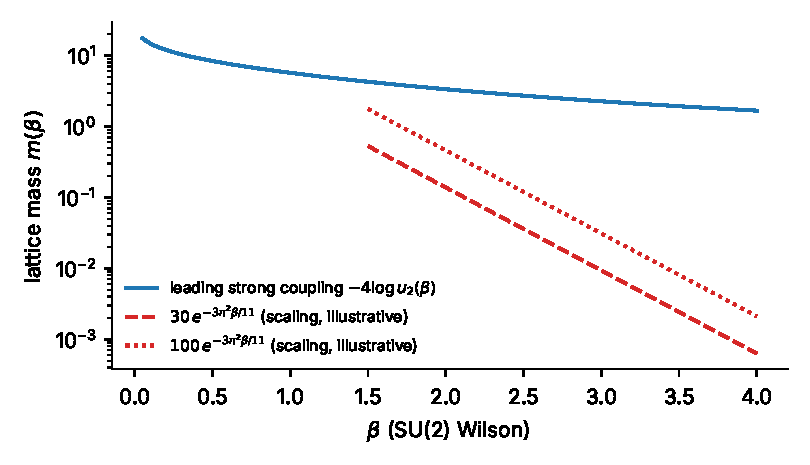
\includegraphics[width=0.92\textwidth]{figures/strong_vs_scaling.pdf}
\caption[The two ends of the coupling range for SU(2)]{The two ends of the coupling range for SU(2). The leading strong coupling mass $-4\log u_2(\beta)$ is controlled by the cluster expansion for small $\beta$. The continuum limit requires the scaling behaviour $m(\beta)\propto e^{-3\pi^2\beta/11}$ as $\beta\to\infty$; the prefactors shown are illustrative. The mass gap problem lives in the crossover between them.}
\label{fig:strongscaling}
\end{figure}

\subsection{What would bridge the gap}

The two dimensional proof of Chapter~\ref{ch:twod} suggests the shape of what is needed. There, an explicit transfer matrix\index{transfer matrix} eigenvalue was bounded at every coupling by a special function inequality whose weak coupling behaviour exactly matched the conversion to physical units. In four dimensions we would like a lower bound
\[
m(\beta)\ge f(\beta)\quad\text{for all }\beta,\qquad\liminf_{\beta\to\infty}\frac{f(\beta)}{a(\beta)}>0 .
\]
We call this a transfer matrix Bessel inequality. Strong coupling supplies it for $\beta<\beta_0$, and asymptotic freedom\index{asymptotic freedom} says what $f$ must look like for large $\beta$. The difficulty is everything in between.

Renormalization group methods are the classical tool for crossing scales. Ba\l aban\index{Balaban, T.@Ba\l aban, T.}'s rigorous renormalization group for lattice gauge theory\cite{Ba87} controls the theory at weak coupling, at short distances, and in the later papers of the series proves ultraviolet stability. What it does not do is follow the flow into the strong coupling regime at long distances, where the gap is generated. Section~\ref{ch:mk} studies a renormalization group that can be followed all the way, at the price of an approximation, and reads it through the probabilistic toolkit.

\section{Lattice Monte Carlo for Glueballs}\label{ch:latticemc}\index{glueball}\index{heat bath}\index{overrelaxation}\index{smearing}

The predictions of the Migdal Kadanoff ladder, and the gap estimator of Chapter~\ref{ch:estimation}, both need lattice data at intermediate and weak coupling. This section describes how glueball correlators are measured in four dimensions and where the statistical difficulties lie.

\subsection{Updates}

For SU(2) the standard update is the heat bath of Creutz\cite{Cr80}, in the Kennedy and Pendleton form\cite{KP85} at weak coupling, which samples each link exactly from its von Mises Fisher conditional (Section~\ref{ch:latent}). For SU(3) the Cabibbo and Marinari~\cite{CM82} method applies the SU(2) heat bath to a sequence of SU(2) subgroups. Overrelaxation reflects each link through the direction of its staple sum, leaving the action unchanged; it is microcanonical and must be combined with heat bath steps, but it reduces autocorrelations substantially. Hybrid Monte Carlo~\cite{DKPR87} moves all links together along Hamiltonian trajectories and is the method of choice when fermions are present; for pure gauge theory the heat bath and overrelaxation combination remains very efficient.

Figure~\ref{fig:plaqhist} shows the output of our own four dimensional heat bath, used in Chapter~\ref{ch:progress}: plaquette histories on an $8^4$ lattice at five couplings, and their autocorrelations, which die out within a few sweeps. The plaquette is the easiest observable; glueball correlators, discussed next, are far noisier.

\begin{figure}[t]
\centering
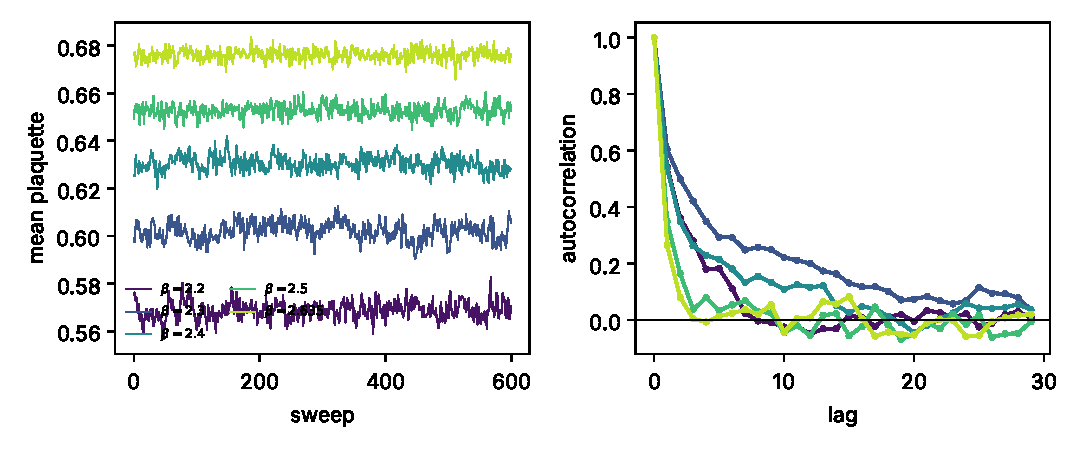
\includegraphics[width=0.95\textwidth]{figures/plaquette_history.pdf}
\caption[Four dimensional SU(2) plaquette histories]{Mean plaquette histories over six hundred heat bath sweeps on an $8^4$ lattice at five couplings (left) and their autocorrelation functions (right).}
\label{fig:plaqhist}
\end{figure}

\subsection{Glueball operators}

A glueball operator is a gauge invariant combination of Wilson loops at a fixed time, summed over space to project onto zero momentum, with the combination chosen to transform in an irreducible representation of the cubic group and of parity and charge conjugation. The scalar $0^{++}$ uses sums of plaquettes; the tensor $2^{++}$ uses differences of plaquette orientations. Because the lightest glueball mass in lattice units is of order one or below at accessible couplings, its correlator falls below the noise within a few time slices. Three techniques are essential.
\begin{itemize}
\item Smearing replaces each spatial link by an average over paths, as in APE~\cite{APE87} or stout smearing~\cite{MP04}, so that operators are extended objects with better overlap on the ground state.
\item Variational analysis builds a matrix of correlators $C_{ij}(\tau)$ from many operators and solves the generalised eigenvalue problem $C(\tau)v=\lambda(\tau,\tau_0)C(\tau_0)v$. The eigenvalues decay with the masses of the lowest states, separating them. In the language of this book, this is a matrix version of the spectral measure, and its positivity is reflection positivity of the matrix valued correlator.
\item Anisotropic lattices use a finer spacing in time than in space, giving more time slices before the signal is lost, as in Morningstar and Peardon's\cite{MP} glueball spectrum.
\end{itemize}

\subsection{The signal to noise problem}

The variance of a glueball correlator does not decay with $\tau$, because $|O|^2$ has a vacuum expectation value, while the signal decays like $e^{-m\tau}$. The signal to noise ratio therefore falls exponentially. L\"uscher and Weisz\cite{LW01} introduced multilevel algorithms, which exploit the locality of the action to average sub lattices independently with the boundary fixed, reducing the variance exponentially in the number of levels.

\subsection{Topological freezing and open boundaries}

At fine lattice spacing the topological charge freezes, as shown for two dimensional U(1) in Figure~\ref{fig:u1}. Schaefer, Sommer and Virotta~\cite{SSV11} showed the effect in four dimensional SU(3) and its influence on other observables. L\"uscher and Schaefer~\cite{LS11} proposed open boundary conditions in time, which let topological charge flow in and out of the lattice and remove the barrier. Other remedies include parallel tempering in boundary conditions and density of states methods\cite{LLR}; split sampling by topological sector (Section~\ref{ch:vertical}) is a candidate that we have not tested.

\subsection{From data to the gap}

The output of a glueball computation is a set of correlators at a few couplings, each with an estimated lattice mass and its uncertainty, typically with autocorrelations estimated by the Madras and Sokal\cite{MS88} windowing of Section~\ref{ch:sokal}. Chapter~\ref{ch:estimation} proposed estimating the gap as a support constraint on a positive measure, and noted that local rates and the profile estimate err toward a larger gap, so that data bound the true gap from above. The Migdal Kadanoff ladder predicts the lattice mass as a function of the coupling, through the number of steps to strong coupling. Comparing that prediction with published lattice masses\cite{MP,Te98} is a test of the caricature, and therefore of the plausibility of the comparison step on which the path of Chapter~\ref{ch:path} depends.

\section{The Migdal Kadanoff Ladder}\label{ch:mk}

In 1975 Migdal\cite{Mi75} proposed a renormalization group for lattice gauge theories that is simple enough to iterate to arbitrarily long distances. Kadanoff\cite{Ka75,Ka76} explained it as a combination of two moves on the lattice, and showed that one of them is exact in two dimensions and the other gives one sided bounds. This section reads the recursion probabilistically: it alternates a Bayesian product of likelihoods with a convolution of laws on the group. Flat space would make the coupling marginal in four dimensions. The curvature of the group makes it run, and the size of the effect is the mean of the Biane Pitman Yor\index{Biane Pitman Yor variable}\cite{BPY} variable $S_{\mathrm{BPY}}$.

\subsection{Bond moving and decimation}

Consider a hypercubic lattice in $d$ dimensions and a scale factor $b\ge2$. One Migdal Kadanoff\index{Migdal Kadanoff recursion} step does two things to every plaquette weight $f$.
\begin{enumerate}
\item[(i)] Bond moving. In each plane, the plaquettes in a $b\times b$ block are moved, in the $d-2$ transverse directions, onto a single plane, so each surviving plaquette carries $k=b^{d-2}$ copies of the original weight: $f\mapsto f^{\,k}$.
\item[(ii)] Decimation. In that plane, the $b\times b$ block of strengthened plaquettes is glued into one by integrating out the interior links. As in two dimensions, this is a convolution of class functions, and in character variables $u_n\mapsto u_n^{\,b^2}$.
\end{enumerate}
After the step the lattice spacing is $ba$. On the hierarchical lattice built by iterating these two moves, the recursion is exact. On $\Z^d$ it is an approximation, and bond moving\index{bond moving} is where the approximation enters. Kadanoff showed that moving bonds in one direction raises, and in the other lowers, the free energy, which gives one sided bounds that we discuss in Chapters~\ref{ch:path} and~\ref{ch:sandwich}.

\subsection{A probabilistic reading}

Normalise the plaquette weight to a probability density $f$ with respect to Haar measure\index{Haar measure} on SU(2). Then:
\begin{itemize}
\item Bond moving replaces $f$ by $f^k/\int f^k$. This is the posterior obtained by combining $k$ independent copies of the likelihood $f$ for an unknown group element, starting from the flat Haar prior. It is a Bayesian product.
\item Decimation replaces $f$ by the $b^2$ fold convolution $f^{*b^2}$. This is the law of a product of $b^2$ independent random group elements with law $f$. For Brownian laws it adds times.
\end{itemize}
So one step of the renormalization group is a product followed by a convolution. In the language of Polson and Scott's\cite{PSdual} duality between envelopes and mixtures, bond moving is an envelope and decimation\index{decimation} is a mixture.

\begin{lemma}[positivity is preserved]\label{lem:posB}
If $f$ has nonnegative character coefficients, so does its image under one Migdal Kadanoff step.
\end{lemma}

\begin{proof}
Decimation raises the coefficients to the power $b^2$. For bond moving, the Clebsch Gordan\index{Clebsch Gordan rule} rule for SU(2),
\[
\chi_p\chi_n=\sum_{j=|p-n|+1,\ \text{step }2}^{p+n-1}\chi_j,
\]
has every multiplicity equal to one, hence nonnegative. So products of class functions with nonnegative coefficients have nonnegative coefficients, and so do powers. For general compact groups the same holds because tensor product multiplicities are nonnegative integers.
\end{proof}

By the Bochner theorem of Chapter~\ref{ch:positivity} (Proposition~\ref{prop:bochnergroup}), nonnegative coefficients are positive definiteness, which is the Osterwalder Seiler condition for reflection positivity\index{reflection positivity}. Every rung of the ladder is therefore the $\Z^4$ lattice theory with that plaquette weight, which is reflection positive with genuine nonnegative spectral measure\index{spectral measure}s, and the tools of Sections~\ref{ch:routeA} and~\ref{ch:routeB} apply at each rung.

\subsection{The Gaussian ledger}

At weak coupling the plaquette law is concentrated near the identity, where the group looks like its Lie algebra $\R^3$. Suppose for a moment that the law were exactly Gaussian on $\R^3$ with precision $\rho$ per coordinate. Then the two operations act by simple arithmetic:
\[
\text{bond moving: }\rho\mapsto k\rho,\qquad\text{decimation: }\rho\mapsto \rho/b^2 .
\]
With $k=b^{d-2}$ the net effect is $\rho\mapsto b^{d-4}\rho$. In two dimensions the precision falls by $b^2$ per step, which is the exact decimation of Chapter~\ref{ch:twod}. In three dimensions it falls by $b$. In four dimensions it is unchanged: the coupling is marginal. Whatever makes the four dimensional coupling run must come from the departure of the group from flat space.

\subsection{Curvature and the Biane Pitman Yor variable}

The departure is visible in the small time form of the heat kernel\index{heat kernel} from Chapter~\ref{ch:twod},
\[
K_t(\theta)\approx C\,t^{-3/2}\,\frac{\theta}{\sin\theta}\,e^{-\theta^2/t}.
\]
The Gaussian part has precision proportional to $1/t$; the factor $\theta/\sin\theta$ is the curvature correction. Raising to the power $k$,
\[
K_t^k\propto\Big(\frac{\theta}{\sin\theta}\Big)^{k-1}\cdot\frac{\theta}{\sin\theta}\,e^{-k\theta^2/t}\propto\Big(\frac{\theta}{\sin\theta}\Big)^{k-1}K_{t/k}(\theta).
\]
The extra factor $(\theta/\sin\theta)^{k-1}$ is the whole of the correction. Continue it to imaginary angle, $\theta=ix$:
\[
\Big(\frac{x}{\sinh x}\Big)^{k-1}=\E\exp\Big(-\frac{x^2}{2}\sum_{j=1}^{k-1}S_{\mathrm{BPY},j}\Big),
\]
where the $S_{\mathrm{BPY},j}$ are independent copies of the Biane Pitman Yor variable with Laplace transform $\sqrt{2\lambda}/\sinh\sqrt{2\lambda}$. To second order in $x$ this is $\exp(-(k-1)\E S_{\mathrm{BPY}}\,x^2/2)$, and returning to real angle the curvature factor is a Gaussian tilt $\exp((k-1)\E S_{\mathrm{BPY}}\,\theta^2/2)$ that removes precision.

\begin{figure}[t]
\centering
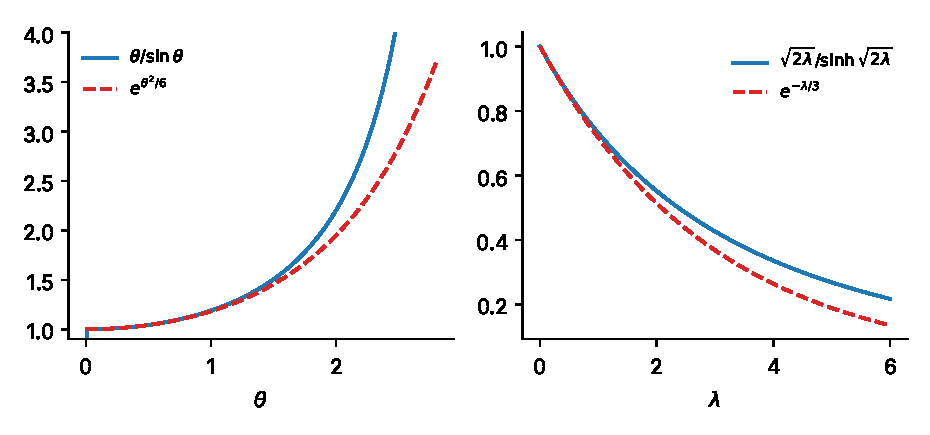
\includegraphics[width=\textwidth]{figures/curvature_bpy.pdf}
\caption[Left: the curvature factor $\theta/\sin\theta$ and its Gaussian approximation $e^{\theta^2/6}$]{Left: the curvature factor $\theta/\sin\theta$ and its Gaussian approximation $e^{\theta^2/6}$. Right: at imaginary angle the same factor is the Laplace transform $\sqrt{2\lambda}/\sinh\sqrt{2\lambda}$ of the Biane Pitman Yor variable $S_{\mathrm{BPY}}$, compared with $e^{-\lambda\E S_{\mathrm{BPY}}}=e^{-\lambda/3}$.}
\label{fig:curvatureB}
\end{figure}

\begin{remark}[leading order derivation: the decrement]\label{prop:decrementB}
For the heat kernel action with small $t=2/\beta$, one Migdal Kadanoff step with scale $b$ in dimension $d$ maps $t$ to $t''$ with
\[
\frac1{t''}=\frac{b^{d-4}}{t}-\frac{(b^{d-2}-1)\,\E S_{\mathrm{BPY}}}{2b^2}+O(t).
\]
In four dimensions,
\[
\beta''=\beta-\big(1-b^{-2}\big)\E S_{\mathrm{BPY}}+O(1/\beta)=\beta-\frac{b^2-1}{3b^2}+O(1/\beta).
\]
This is a leading order derivation: the Gaussian approximation of $\theta/\sin\theta$ is made without bounding the $O(t)$ and $O(1/\beta)$ remainders, so the remainders are not proved to be of that order.
\end{remark}

\begin{proof}[Derivation]
Write the heat kernel near the identity as a Gaussian of precision $2/t$ in $\theta$, times the curvature factor. Bond moving multiplies the Gaussian precision by $k$ and multiplies the law by $(\theta/\sin\theta)^{k-1}\approx e^{(k-1)\E S_{\mathrm{BPY}}\,\theta^2/2}$, so the new precision is $2k/t-(k-1)\E S_{\mathrm{BPY}}$, that is $1/t'=k/t-(k-1)\E S_{\mathrm{BPY}}/2$. Decimation divides the precision by $b^2$. With $k=b^{d-2}$ this gives the first formula, and with $d=4$ and $\beta=2/t$ the second.
\end{proof}

At $b=2$ the decrement is $\frac34\cdot\frac13=\frac14$; at $b=3$ it is $\frac89\cdot\frac13=\frac{8}{27}$. The one loop decrement for SU(2), from Chapter~\ref{ch:problem}, is $\frac{11\ln b}{3\pi^2}$ in units of $\beta$ per step, which is $0.2575$ at $b=2$ and $0.408$ at $b=3$. So at $b=2$ the Migdal Kadanoff coefficient is within three percent of the one loop value. That agreement is specific to $b=2$: as $b\to1$ the Migdal Kadanoff rate per unit $\log b$ tends to $2/3$, against the true $0.3715$. The recursion is a scheme, not an exact computation.

\subsection{SU(N)}

For SU(N) with Wilson weight $\exp(\frac\beta N\operatorname{Re}\operatorname{tr}U)$, write the eigenvalues of a group element as $e^{i\theta_1},\dots,e^{i\theta_N}$ with $\sum\theta_i=0$. Near the identity the Wilson weight is approximately $\exp(-\frac{\beta}{2N}\sum\theta_i^2)$. The Jacobian of the exponential map is a product over positive roots,
\[
j(\theta)^{-1/2}=\prod_{i<j}\frac{(\theta_i-\theta_j)/2}{\sin\big((\theta_i-\theta_j)/2\big)},
\]
so the curvature factor is a product of $N(N-1)/2$ Biane Pitman Yor factors. Using
\[
\sum_{i<j}(\theta_i-\theta_j)^2=N\sum_i\theta_i^2\qquad\text{when }\sum_i\theta_i=0,
\]
the tilt is isotropic and the Gaussian ledger closes exactly as for SU(2).

\begin{remark}[leading order derivation: the SU(N) decrement]\label{prop:sunB}
At weak coupling one Migdal Kadanoff step in four dimensions gives
\[
\beta''=\beta-\big(1-b^{-2}\big)\frac{N^2}{4}\,\E S_{\mathrm{BPY}}+O(1/\beta)=\beta-\big(1-b^{-2}\big)\frac{N^2}{12}+O(1/\beta).
\]
The one loop decrement is $\frac{11N^2\ln b}{12\pi^2}$, so the ratio of the two is $\frac{\pi^2(1-b^{-2})}{11\ln b}$, independent of $N$. At $b=2$ it equals $\frac{12\pi^2}{176\ln2}=0.971$. As for the SU(2) case, the remainder is not bounded.
\end{remark}

\begin{proof}[Derivation]
In terms of $c=\beta/N$, the Gaussian precision per coordinate $\theta_i$ is $c$. Bond moving gives $kc$ minus the tilt $(k-1)\E S_{\mathrm{BPY}}\cdot\frac14\cdot N$, from $\sum_{i<j}\frac{(\theta_i-\theta_j)^2}{4}=\frac N4\sum\theta_i^2$. Decimation divides by $b^2$. With $k=b^2$ and $\beta=Nc$ the stated decrement follows, and for $N=2$ it reduces to Remark~\ref{prop:decrementB}.
\end{proof}

We checked Remark~\ref{prop:sunB} for SU(3) numerically, in double precision, with a full computation: class functions on the maximal torus, the Weyl character formula\index{Weyl character formula} on a $192\times192$ grid, $1081$ irreducible representations, and the coupling defined by matching the fundamental character coefficient to the Wilson action\index{Wilson action}. The decrement is $0.581$, $0.572$, $0.569$ and $0.568$ at $\beta=12,16,20,24$, approaching $9/16=0.5625$ at rate $1/\beta$ (Figure~\ref{fig:su3B}). The one loop value is $0.5794$.

\begin{figure}[t]
\centering
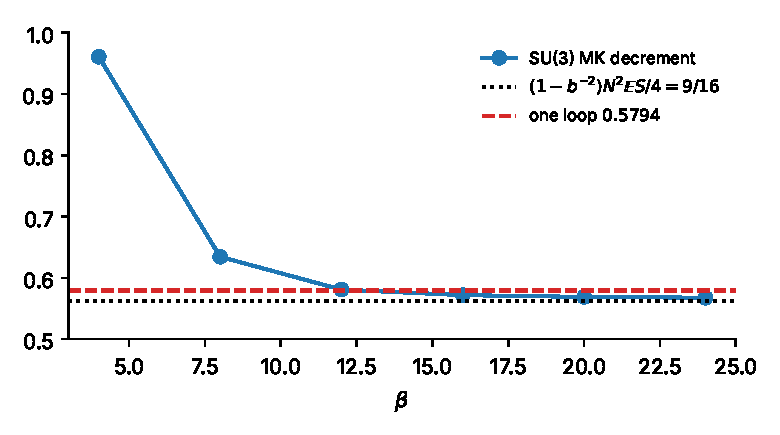
\includegraphics[width=0.9\textwidth]{figures/su3_decrement.pdf}
\caption[SU(3) Migdal Kadanoff decrement per step at $b=2$, from a full computation with Weyl characters]{SU(3) Migdal Kadanoff decrement per step at $b=2$, from a full computation with Weyl characters. It approaches the prediction $9/16$ of Remark~\ref{prop:sunB}, three percent below the one loop value.}
\label{fig:su3B}
\end{figure}

\subsection{The full flow for SU(2)}

We ran the recursion for SU(2) with $b=2$ and $d=4$, starting from the Wilson action, in double precision floating point, with class functions represented by up to $1500$ characters and $6000$ point Gauss Legendre quadrature. Apart from the proved Lemma~\ref{lem:mlrB} and Proposition~\ref{prop:criterionB}, this section and the next are numerical results: nothing else in them carries an enclosure or an interval bound. The code reproduces $I_n/I_1$ for $n=2,3$ at $\beta=3$ to double precision. Figure~\ref{fig:mklevelsB} follows the Thorin levels $u_n$ along a trajectory started at $\beta=6$. They stay close to one for about twenty steps while the coupling drifts down, then collapse together within a few steps as the flow enters strong coupling.

\begin{figure}[t]
\centering
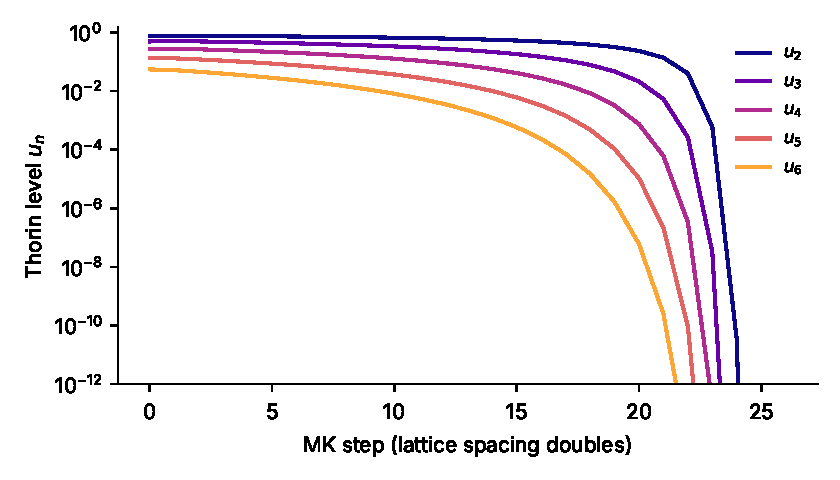
\includegraphics[width=0.9\textwidth]{figures/mk_levels.pdf}
\caption[Thorin levels $u_n$ along the SU(2) Migdal Kadanoff flow from the Wilson action at $\beta=6$]{Thorin levels $u_n$ along the SU(2) Migdal Kadanoff flow from the Wilson action at $\beta=6$. Each step doubles the lattice spacing. The slow drift followed by a sudden collapse is the logarithmic running of asymptotic freedom followed by the onset of confinement.}
\label{fig:mklevelsB}
\end{figure}

Defining the effective coupling $\beta_{\mathrm{eff}}$ by matching $u_2$ to the Wilson value, the flow has the following features (Figure~\ref{fig:mkflowB}).
\begin{itemize}
\item For initial $\beta\ge2$ the first step from the Wilson action raises $\beta_{\mathrm{eff}}$, by between $0.1$ and $0.37$. The Wilson action is not on the renormalized trajectory, and the first step appears to project onto it.
\item After the first step the decrement is positive along every trajectory and at every coupling sampled. It peaks at about $0.42$ near $\beta_{\mathrm{eff}}\approx0.8$, the crossover, and tends to $0.249+0.032/\beta$ at weak coupling.
\item Every initial coupling sampled reaches strong coupling. The number of doublings needed grows like $3.98\,\beta$, against $4$ from Remark~\ref{prop:decrementB} and $3.88$ from one loop asymptotic freedom.
\end{itemize}
\begin{center}
\begin{tabular}{rcc}
\toprule
initial $\beta$ & $\beta_{\mathrm{eff}}$ after one step & doublings to $u_2<0.02$ \\ \midrule
2 & 2.109 & 7 \\
4 & 4.305 & 15 \\
8 & 8.354 & 31 \\
16 & 16.366 & 63 \\
24 & 24.370 & 94 \\
\bottomrule
\end{tabular}
\end{center}


\begin{figure}[t]
\centering
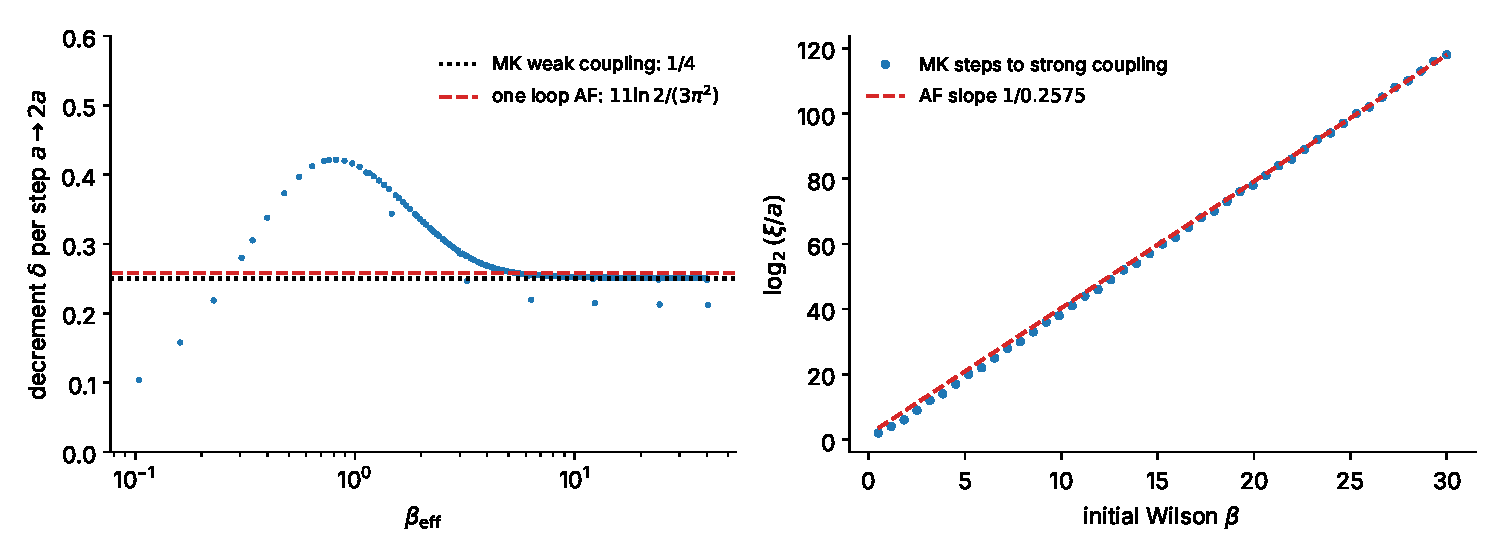
\includegraphics[width=\textwidth]{figures/mk_flow.pdf}
\caption[SU(2) Migdal Kadanoff flow from the Wilson action]{SU(2) Migdal Kadanoff flow from the Wilson action. Left: the decrement per step along six trajectories. Right: the number of doublings to strong coupling is linear in $\beta$, with a slope close to the one loop value of asymptotic freedom.}
\label{fig:mkflowB}
\end{figure}

In the computed flows there is no fixed point at finite coupling, and every coupling flows to confinement\index{confinement}. This is Migdal's original observation, and on the hierarchical lattice where the recursion is exact, Ito\index{Ito, K. R.}\cite{Ito85} proved confinement at all couplings in 1985. What the probabilistic reading adds is an explanation of the rate, through a single number, the mean of a generalized gamma convolution\index{generalized gamma convolution}\cite{Bo92}, together with the positivity of every rung. Section~\ref{ch:verification} sets the numerical observation that the decrement is positive beside a one dimensional map and a proved inequality.

\section{Checking the Ladder}\label{ch:verification}

Section~\ref{ch:mk} observed that the Migdal Kadanoff\index{Migdal Kadanoff recursion} coupling decreases at every step. This section states the observation for an explicit one dimensional map and records exactly what was computed, proves the monotonicity that the check needs from a likelihood ratio\index{likelihood ratio order} property of the heat kernel\index{heat kernel}, and reads the correlation length as a first passage time\index{first passage time}.

\subsection{The heat kernel projected map}

The full recursion acts on an infinite sequence of character coefficients. To obtain a one dimensional map we project onto the heat kernel family after each step.

\begin{definition}
For $\beta>0$ let $t=2/\beta$ and start from the heat kernel law $u_n=e^{-t(n^2-1)/4}$. Apply one Migdal Kadanoff step with $b=2$ and $d=4$, read off the new second coefficient $u_2''$, and define $R(\beta)=2/t''$ where $u_2''=e^{-3t''/4}$.
\end{definition}

Starting from the heat kernel removes the first step anomaly of the Wilson action\index{Wilson action}. The projection is a definition, and the exact recursion acts on all character coefficients. The following checks, all in double precision, test the projection and the map numerically.
\begin{itemize}
\item Reducing the number of characters from $1500$ to $800$ and the number of quadrature points from $6000$ to $4000$ changes $R$ by less than $10^{-11}$ on the tested points.
\item Iterating $R$ reproduces the unprojected flow, started from the same heat kernel law, to within $0.012$ over eight steps from $\beta=3$, and to within $0.003$ from $\beta=10$.
\item At $b=3$ (the same projection with $b=3$) the decrement $\beta-R(\beta)$ is $0.2974$, $0.2969$ and $0.2966$ at $\beta=10,20,40$, approaching $8/27=0.2963$ as Remark~\ref{prop:decrementB} predicts.
\end{itemize}
At $b=2$ the decrement is $0.2726$ at $\beta=0.5$, $0.2806$ at $\beta=1$, $0.2623$ at $\beta=2$, $0.2544$ at $\beta=5$, $0.2521$ at $\beta=10$ and $0.2504$ at $\beta=50$. Above $\beta=20$ it fits $0.25000+0.021/\beta$.

\subsection{Monotonicity from a likelihood ratio}

\begin{lemma}\label{lem:mlrB}
Suppose the SU(2) heat kernel has monotone likelihood ratio in time, meaning that $\partial_\theta\log K_t(\theta)$ is increasing in $t$ for every $\theta\in(0,\pi)$. Then $R$ is increasing.
\end{lemma}

\begin{proof}
After bond moving\index{bond moving}, the second normalised character coefficient is $u_2=\E_{\nu_t}[\cos\theta]$, where $\nu_t\propto K_t^k$ times the Haar density, because $\chi_2(\theta)/2=\cos\theta$. Monotone likelihood ratio passes from $K_t$ to $K_t^k$, since $\partial_\theta\log K_t^k=k\,\partial_\theta\log K_t$. By Proposition~\ref{prop:lro}(i) of Section~\ref{ch:toolkit}, $\nu_{t'}$ is then stochastically larger than $\nu_t$ for $t'>t$, so $\E_{\nu_t}\cos\theta$ is decreasing in $t$. Decimation $u\mapsto u^{b^2}$ and the conversion back to $\beta$ are increasing, and $t=2/\beta$ is decreasing in $\beta$. Composing, $R$ is increasing.
\end{proof}

The hypothesis is a theorem: Corollary~\ref{cor:mlrall} of Chapter~\ref{ch:progress} proves it at every time from a product formula for the heat kernel. We keep the original evidence, which is independent of that proof. The hypothesis holds asymptotically at both ends of the time range. For small $t$ the image sum of Chapter~\ref{ch:twod} gives $\partial_\theta\log K_t(\theta)\approx-2\theta/t+1/\theta-\cot\theta$; the leading term $-2\theta/t$ is increasing in $t$, and the corrections are exponentially small in $1/t$ away from $\theta=\pi$. For large $t$ the leading nontrivial mode gives $\partial_\theta\log K_t(\theta)\approx-4e^{-3t/4}\sin\theta$, which is increasing in $t$ because $\sin\theta>0$. In between we checked it numerically, in double precision, on an $800\times1500$ grid of $(t,\theta)$ with $t\in[0.004,40]$. For $t<2$ we used the Poisson resummed image sum, which avoids the catastrophic cancellation that afflicts the character series at small times. For $t\ge2$ we used the character series. The two agree to $3\times10^{-10}$ at $t=2$. At every grid point no computed increment in $t$ is below $-10^{-12}$. This is a floating point check, not an enclosure.

\subsection{The covering argument}

\begin{remark}[numerical result: covering]\label{prop:coverB}
The inequality $R(\beta)<\beta$ is proved for every $\beta>0$ as Corollary~\ref{cor:contracts}. What is recorded here is the floating point computation that preceded the proof. It is a statement in heat kernel coordinates: one exact rung from a Wilson law can raise the fundamental coefficient, as Table~\ref{tab:notmonotone} of Chapter~\ref{ch:counts} shows. We computed $R$ in IEEE double precision, with truncated character series and Gauss Legendre quadrature, with no interval arithmetic and no allowance for rounding, on a grid of $1899$ points in $[0.3,300]$: $400$ geometrically spaced points in $[0.3,2]$ and $1500$ equally spaced points in $[2,300]$. On this grid the computed $R$ is increasing and satisfies $R(\beta_{i+1})<\beta_i$ for every consecutive pair, with smallest computed margin $0.051$. Granted the monotonicity of Lemma~\ref{lem:mlrB}, the argument below then gives $R(\beta)<\beta$ on $[0.3,300]$, up to floating point and truncation error. The margin is far larger than the changes of order $10^{-11}$ seen when the truncation is reduced, but that is evidence and not an enclosure.
\end{remark}

\begin{proof}[Argument]
For $\beta\in[\beta_i,\beta_{i+1}]$, monotonicity gives $R(\beta)\le R(\beta_{i+1})<\beta_i\le\beta$.
\end{proof}

\begin{figure}[t]
\centering
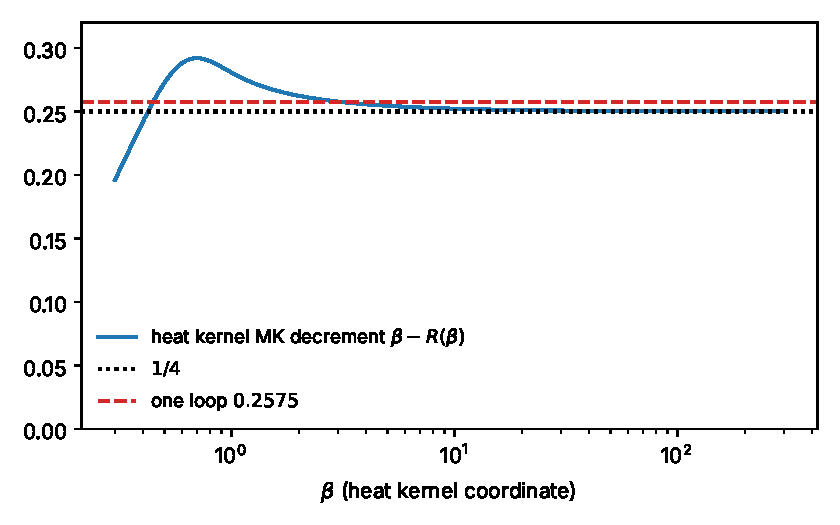
\includegraphics[width=0.85\textwidth]{figures/mk_cover.pdf}
\caption[The decrement $\beta-R(\beta)$ of the heat kernel projected Migdal Kadanoff map for SU(2)]{The decrement $\beta-R(\beta)$ of the heat kernel projected Migdal Kadanoff map for SU(2), computed in double precision on the grid of the covering computation. It is positive throughout, peaks near the crossover, and tends to $(1-b^{-2})\E S_{\mathrm{BPY}}=1/4$, slightly below the one loop value.}
\label{fig:coverB}
\end{figure}

The computed decrement lies in $[0.196,0.292]$ on the grid, with its maximum near $\beta\approx0.7$. Below $\beta=0.38$ we have $u_2<0.02$. We use this as the working definition of strong coupling for the ladder. We know no explicit convergence radius for a cluster expansion in these coordinates: the Osterwalder Seiler theorem gives an unspecified $\beta_0$ for the Wilson action, and after several steps the weight is a general class function, so we do not claim that the grid overlaps a region where the cluster expansion\index{cluster expansion} converges. Above $\beta=300$ the asymptotics of Remark~\ref{prop:decrementB}, with a positive $O(1/\beta)$ correction fitted at $0.021/\beta$, are a leading order derivation and a fit, not a bound. A computer assisted theorem on a grid would need interval arithmetic for $R$ at the grid points, interval arithmetic for the likelihood ratio inequality, and an explicit bound on the $O(1/\beta)$ remainder. Each is a finite computation with explicit, smooth functions, and none has been done here. The enclosures with an explicit rounding allowance are those of Chapter~\ref{ch:progress}.

\subsection{The correlation length as a first passage time}

Define the renormalization walk $\beta_{\ell+1}=R(\beta_\ell)$ of the projected map and its first passage time below the strong coupling threshold,
\[
J(\beta)=\min\{\ell:\beta_\ell<\beta_*\},\qquad\beta_*=0.38 .
\]
Each step multiplies the lattice spacing by $b$, so lengths measured in units of the original spacing are $b^{J}$ times lengths on the final lattice. If $\xi_*$ is the correlation length of the strong coupling theory reached after $J$ steps (at a coupling below $\beta_*$ that depends on $\beta$), and if the projected walk stands for the true recursion, then
\[
\xi(\beta)=b^{J(\beta)}\,\xi_* .
\]
The telescoping identity $\beta-\beta_J=\sum_{\ell<J}\delta(\beta_\ell)$, with $\delta(\beta)=\beta-R(\beta)$, is a deterministic form of Wald\index{Wald identity}'s identity:
\[
J(\beta)=\frac{\beta-\beta_J}{\bar\delta_J},
\]
where $\bar\delta_J$ is the average decrement along the path. If, as the leading order derivation of Remark~\ref{prop:decrementB} suggests, $\delta(\beta)=\delta_\infty+O(1/\beta)$ with $\delta_\infty=(1-b^{-2})\E S_{\mathrm{BPY}}$, the average converges and
\[
\log\xi(\beta)=\frac{\ln b}{(1-b^{-2})\E S_{\mathrm{BPY}}}\,\beta+O(\log\beta).
\]
This is the ladder's form of asymptotic freedom\index{asymptotic freedom}, with the coefficient written as a ratio of $\ln b$ to $(1-b^{-2})$ times the mean of a generalized gamma convolution\index{generalized gamma convolution}. In the Riemann programme~\cite{PS26a} we read the zeros through hitting times of a ladder in the abscissa; here the correlation length is a hitting time of a ladder in the coupling.

\subsection{The gap criterion}

\begin{proposition}[first passage criterion for the projected ladder]\label{prop:criterionB}
For the walk $\beta_{\ell+1}=R(\beta_\ell)$ of the heat kernel projected map, suppose that $R$ is continuous and that
\begin{enumerate}
\item[(A)] $\delta(\beta)>0$ for every $\beta>0$, and
\item[(B)] $\delta(\beta)\to\delta_\infty>0$ with $O(1/\beta)$ corrections.
\end{enumerate}
Then every coupling reaches the strong coupling region $\beta<\beta_*$ in $J(\beta)=\beta/\delta_\infty+O(\log\beta)$ steps.
\end{proposition}

\begin{proof}
Condition (A), with continuity and the asymptotics (B), bounds $\delta$ below by a positive constant on $[\beta_*,\infty)$, so $J(\beta)<\infty$ and the estimate on $J$ follows by summing.
\end{proof}

The proposition is about the projected map and says nothing yet about a gap. To reach the gap on the Migdal Kadanoff hierarchical lattice, at least three further things are needed, and none is proved here.

\begin{remark}[what the criterion would give for the gap]
Suppose in addition that (C) the exact recursion on the hierarchical lattice is described by the projected map, so that the steps above are steps of the true flow; (D) the theories reached after $J(\beta)$ steps, which sit at couplings below $\beta_*$ that vary with $\beta$, have a positive lattice mass bounded below by a constant $m_*$ uniformly in $\beta$, which is a cluster expansion statement with explicit constants; and (E) in physical units, where $a(\beta)$ is the physical lattice spacing of the real theory, $a(\beta)\Lambda\propto\exp(-3\pi^2\beta/11)$ at one loop times a power of $\beta$ from the two loop term, the product $a(\beta)\,b^{J(\beta)}$ is bounded as $\beta\to\infty$. Then the correlation length of the hierarchical lattice theory is at most $b^{J(\beta)}/m_*$ in lattice units, hence bounded in physical units. That is a bound on a correlation length. It is not the uniform Thorin gap inequality: the hierarchical lattice has no spectral measures (see the end of this remark), and Theorem~\ref{thm:equivB} would need in addition nonnegative measures $\mu^{(a)}$ with $\sup_a\int e^{-\alpha_0E}\,d\mu^{(a)}$ finite and uniformity in the volume, which are the two missing steps recorded after the Osterwalder and Seiler theorem above. The status of the three conditions is as follows. (C) is open: the exact recursion acts on all character coefficients, and the agreement of the two is numerical only ($0.012$ over eight steps). (D) is open: no explicit convergence radius is known to us, nor a lower bound on the mass uniform on $(0,\beta_*]$. (E) is not merely open: as stated it fails for the ladder with $\delta_\infty=\frac14$ ($b=2$): $b^{J(\beta)}$ grows like $\exp(4\ln2\,\beta)=\exp(2.773\,\beta)$ while the one loop $a(\beta)$ decays like $\exp(-2.692\,\beta)$, so the product grows like $\exp(0.081\,\beta)$ times a power, because the Migdal Kadanoff decrement differs from the one loop value $0.2575$ (Remark~\ref{prop:decrementB}). Only with the ladder's own scale $a_{\mathrm{lad}}(\beta)=b^{-J(\beta)}$ is (E) close to the definition of $J$, and then no two loop term enters. So the conclusion of this remark is conditional on a scale matching that the ladder does not supply. If $\delta(\beta)=\delta_\infty+c/\beta$ then summing gives $J(\beta)\approx\beta/\delta_\infty-(c/\delta_\infty^2)\ln\beta$, so the sign and size of the logarithmic term, set against the power of $\beta$ in $a(\beta)$, would decide whether the product is bounded if the exponential rates agreed. Lemma~\ref{lem:posB} gives reflection positivity of the $\Z^4$ theory whose plaquette weight is a given rung. It does not give reflection positivity, a transfer matrix or spectral measures for the hierarchical lattice, so the Thorin densities of the hierarchical flow are not defined by it.
\end{remark}

Condition (B) is the leading order derivation of Remark~\ref{prop:decrementB}, with the remainder not bounded. Condition (A) for the projected ladder at every coupling is Corollary~\ref{cor:contracts}, which proves $R(\beta)<\beta$; Remark~\ref{prop:coverB} records the floating point evidence on $[0.3,300]$ that preceded it. So for the projected ladder, granted the continuity of $R$, the first passage time is finite at every coupling, and the linear growth of $J$ rests on (B). Confinement itself on the hierarchical lattice is Ito\index{Ito, K. R.}'s 1985 theorem; the criterion above is a statement about the projected map only. What remains is the relation between the projected map and the exact recursion, the relation between the approximation and the real theory, and the strong coupling mass with explicit constants, which are the subjects of Chapters~\ref{ch:path} and~\ref{ch:sandwich}.

\section*{Exercises}
Exercises 1 to 3 refer to Section~\ref{ch:latticemc}, 4 to 7 to Section~\ref{ch:mk}, and 8 to 11 to Section~\ref{ch:verification}.
\begin{enumerate}
\item Show that overrelaxation preserves the action and leaves the Haar measure invariant.
\item Show that the generalised eigenvalue problem recovers the lowest masses exactly when the number of states contributing to the correlator equals the size of the matrix.
\item Explain why the variance of a glueball correlator approaches a constant at large $\tau$.
\item Derive the general formula $1/t''=b^{d-4}/t-(b^{d-2}-1)\E S_{\mathrm{BPY}}/(2b^2)$ in detail, and discuss the cases $d=2$ and $d=3$.
\item Verify the identity $\sum_{i<j}(\theta_i-\theta_j)^2=N\sum_i\theta_i^2$ when $\sum_i\theta_i=0$.
\item Show that for SU(2), $\chi_2(\theta)/2=\cos\theta$, and hence that $u_2=\E[\cos\theta]$ under the normalised plaquette law.
\item Compute the ratio $\pi^2(1-b^{-2})/(11\ln b)$ for $b=2,3,4$ and explain why the Migdal Kadanoff coefficient depends on $b$.
\item Show that if $R$ is increasing and $R(\beta_{i+1})<\beta_i$ for consecutive grid points, then $R(\beta)<\beta$ on the whole interval, and explain why a floating point check of the grid inequality is not an enclosure.
\item Using the image sum, prove the likelihood ratio property of the SU(2) heat kernel for all sufficiently small $t$.
\item Estimate the number of Migdal Kadanoff steps from $\beta=10$ to strong coupling using only the asymptotic decrement, and compare with the table of doublings in Section~\ref{ch:mk}, interpolating between $\beta=8$ and $\beta=16$.
\item Explain why projecting onto the heat kernel family after each step, rather than following all character coefficients, changes the trajectory by only a small amount at weak coupling.
\end{enumerate}

\chapter{The Ladder on Counts and Kingman's Coalescent}\label{ch:counts}\index{latent count}\index{coalescence}\index{complete monotonicity}

Chapter~\ref{ch:strong} built the Migdal Kadanoff ladder and its projected form, and left open what the exact ladder, without the projection, does to a link density. The heat kernel and the Wilson law are mixtures $\E[(1+\cos\theta)^{M_0}]$ over a random nonnegative integer $M_0$ (Corollary~\ref{cor:Mclosed} below; Section~\ref{ch:langlands} of the later Chapter~\ref{ch:kacyang} returns to this reading). Bond moving adds such counts, and this chapter proves that decimation thins them by a positive kernel. The exact Migdal Kadanoff ladder for SU(2), with no projection, is then a map on the laws of a nonnegative integer, and we can look at it.

\section{The coalescence theorem}

Write $x=\cos\theta$, let $C_n$ be the Catalan numbers, and let
\[
f_j(x)=\frac{2^j}{C_{j+1}}\,(1+x)^j,\qquad j=0,1,2,\dots
\]
be the probability densities with respect to Haar measure. Convolution is on the group.

\begin{theorem}[coalescence]\label{thm:coalescence}
For all integers $a,b\ge0$,
\[
f_a*f_b=\sum_{j=0}^{\min(a,b)}Q(j\mid a,b)\,f_j ,
\]
where $Q(\cdot\mid a,b)$ is a probability law on $\{0,\dots,\min(a,b)\}$ with every weight strictly positive, and
\[
\sum_jj\,Q(j\mid a,b)=\frac{ab}{a+b+2}.
\]
\end{theorem}

The proof has three steps, each elementary.

\begin{lemma}[characters of $f_j$]\label{lem:fjchar}
With $J=j+1$, $f_j=\sum_{n=1}^{J}n\,u_n(J)\,\chi_n$ where
\[
u_n(J)=\frac{(J-1)!\,(J+1)!}{(J-n)!\,(J+n)!}=\frac{J+1}{J}\,\binom{2J}{J-n}\Big/\binom{2J}{J}.
\]
\end{lemma}

\begin{proof}
$2+2\cos\theta=(e^{i\theta/2}+e^{-i\theta/2})^2$, so $(2+2x)^j=\sum_m\binom{2j}{j-m}e^{im\theta}$, and collecting $e^{im\theta}$ into characters $\chi_n=\sum_{|m|<n,\ m\equiv n-1}e^{im\theta}$ gives the coefficient $\binom{2j}{j-n+1}-\binom{2j}{j-n-1}=2n\,(2j+1)!/\big((j-n+1)!\,(j+n+1)!\big)$ of $\chi_n$. Normalise by the coefficient of $\chi_1$.
\end{proof}

So the fundamental coefficient is $u_2=(J-1)/(J+2)=j/(j+3)$, as in Proposition~\ref{prop:latentcount}, and as a function of $n$ the sequence $u_n(J)$ is, up to a constant, the law of the endpoint of a simple random walk of $2J$ steps.

\begin{lemma}[a completely monotone function]\label{lem:cm}
For an integer $N\ge1$ let $w_N(s)=1\big/\big(\Gamma(N+1-\sqrt s)\,\Gamma(N+1+\sqrt s)\big)$. Then
\[
w_N(s)=\frac1{(N!)^2}\prod_{i>N}\Big(1-\frac s{i^2}\Big),
\]
and $(-1)^kw_N^{(k)}(s)>0$ for all $k\ge0$ and $0\le s<(N+1)^2$.
\end{lemma}

\begin{proof}
The product formula follows from $\Gamma(1+z)\Gamma(1-z)=\pi z/\sin\pi z$ and Euler's product for the sine. Each factor is positive, linear and decreasing on $[0,(N+1)^2)$; a finite product of such functions has derivatives of alternating sign by Leibniz's rule, and the signs pass to the limit, which is uniform on compact subsets together with all derivatives.
\end{proof}

\begin{proof}[Proof of Theorem~\ref{thm:coalescence}]
Convolution multiplies the coefficients $u_n$. Put $\bar a=a+1\le \bar b=b+1$ and $g_J(n)=1/\big((J-n)!\,(J+n)!\big)$, so that $u_n(J)=(J-1)!\,(J+1)!\,g_J(n)$. We must write $g_{\bar a}(n)\,g_{\bar b}(n)$, for $n=1,\dots,\bar a$, as a combination of $g_J(n)$, $J=1,\dots,\bar a$, with positive coefficients.

For $J\le \bar a$, $g_J(n)=g_{\bar a}(n)\,P_J(n^2)$ with $P_J(s)=\prod_{i=J+1}^{\bar a}(i^2-s)$, a polynomial of degree $\bar a-J$ that vanishes at $s=n^2$ for $J<n\le \bar a$, as $g_J(n)$ does. And $g_{\bar b}(n)=w_{\bar b}(n^2)$. So it is enough to find $\omega_J$ with
\[
w_{\bar b}(s)=\sum_{J=1}^{\bar a}\omega_J\,P_J(s)\qquad\text{at the nodes }s=1,4,\dots,\bar a^2 .
\]
This is Newton's interpolation formula with the nodes taken in the order $\bar a^2,(\bar a-1)^2,\dots,1$: the basis polynomials are $\prod_{i<k}(s-s_i)=(-1)^kP_{\bar a-k}(s)$, so
\[
\omega_{\bar a-k}=(-1)^k\,w_{\bar b}\big[\bar a^2,(\bar a-1)^2,\dots,(\bar a-k)^2\big],
\]
a divided difference. By the mean value theorem for divided differences it equals $(-1)^kw_{\bar b}^{(k)}(\xi)/k!$ for some $\xi\in[1,\bar a^2]$, which is positive by Lemma~\ref{lem:cm} because $\bar a\le \bar b$. Hence
\[
Q(j\mid a,b)=\omega_J\,\frac{(\bar a-1)!\,(\bar a+1)!\,(\bar b-1)!\,(\bar b+1)!}{(J-1)!\,(J+1)!}>0,\qquad J=j+1 .
\]
The weights sum to one because $u_1=1$ on both sides.

For the mean, use the functional $\mathsf W(f)=\int f(x)\,(1-x)^{-1}$ against Haar measure. Since $\int\chi_n(1-x)^{-1}=\frac2\pi\int_0^\pi\sin n\theta\cot\frac\theta2\,d\theta=2$ for every $n$, $\mathsf W(f)=2\sum_nn\,u_n$. On $f_j$, where $\cos^2(\theta/2)$ is Beta with parameters $j+\frac32,\frac32$, it equals $j+2$. So the mean of $j+2$ under $Q$ is $2\sum_nn\,u_n(\bar a)u_n(\bar b)$. With $d_n=\binom{2\bar a}{\bar a-n}\binom{2\bar b}{\bar b-n}$ one checks $(\bar a+n)(\bar b+n)\,d_n-(\bar a+n+1)(\bar b+n+1)\,d_{n+1}=2n(\bar a+\bar b)\,d_n$, so the sum telescopes:
\[
\sum_{n\ge1}n\,d_n=\frac{(\bar a+1)(\bar b+1)}{2(\bar a+\bar b)}\,d_1,
\]
hence
\[
2\sum_{n\ge1}n\,u_n(\bar a)u_n(\bar b)=\frac{(\bar a+1)(\bar b+1)}{\bar a+\bar b},
\]
and $\frac{(\bar a+1)(\bar b+1)}{\bar a+\bar b}-2=\frac{(\bar a-1)(\bar b-1)}{\bar a+\bar b}=\frac{ab}{a+b+2}$.
\end{proof}

Two small cases: $Q(\cdot\mid1,b)=\big(\frac3{b+3},\frac b{b+3}\big)$ and $Q(\cdot\mid3,3)=\big(\frac5{28},\frac{15}{28},\frac{15}{56},\frac1{56}\big)$. The script \texttt{count\_ladder.py} computes $Q$ in rational arithmetic and confirms positivity and the mean for all $a\le b\le20$; the theorem makes that check redundant, and it was the check that suggested the theorem.

\section{The kernel is hypergeometric}\label{sec:hypergeometric}\index{hypergeometric distribution}\index{Chu Vandermonde identity}

The Newton formula of the last proof hides a closed form. It was found by looking at the numerators of $Q(\cdot\mid3,3)=\frac1{56}(10,30,15,1)$.

\begin{theorem}[the coalescence is an intersection]\label{thm:hypergeometric}
For all $a,b\ge0$ and $0\le j\le\min(a,b)$,
\[
Q(j\mid a,b)=\binom aj\binom{b+2}{b-j}\Big/\binom{a+b+2}{b}.
\]
This is the hypergeometric law: $Q(\cdot\mid a,b)$ is the law of the number of common elements of two independent uniformly random subsets, of sizes $a$ and $b$, of a set of size $a+b+2$.
\end{theorem}

\begin{proof}
We must show $\sum_jQ(j\mid a,b)\,u_n(j+1)=u_n(a+1)\,u_n(b+1)$ for every $n$, with $u_n(j+1)=j!\,(j+2)!/\big((j+1-n)!\,(j+1+n)!\big)$. Substituting, and putting $j=n-1+i$, $a'=a-n+1$, $b'=b-n+1$,
\[
\sum_j\binom aj\binom{b+2}{j+2}u_n(j+1)=\frac{a!\,(b+2)!}{a'!\,b'!\,(2n)!}\sum_{i\ge0}\frac{(-a')_i(-b')_i}{i!\,(2n+1)_i},
\]
and the sum on the right equals
\[
\frac{(a+b+2)!\,(2n)!}{(a+n+1)!\,(b+n+1)!}
\]
by the Chu Vandermonde identity ${}_2F_1(-a',-b';c;1)=(c+b')_{a'}/(c)_{a'}$ with $c=2n+1$. The right side equals $\binom{a+b+2}{b}u_n(a+1)u_n(b+1)$.
\end{proof}

So the theorem of the first section is the Chu Vandermonde identity, and its positivity is the positivity of binomial coefficients. Everything observed about $Q$ now follows at once, and more.

\begin{corollary}\label{cor:hypergeometric}
\begin{enumerate}
\item[(i)] The mean of $Q(\cdot\mid a,b)$ is $ab/(a+b+2)$ and its variance is
\[
\frac{ab\,(a+2)(b+2)}{(a+b+2)^2(a+b+1)} .
\]
\item[(ii)] $Q(j\mid a,b)$ is totally positive of order two in $(j,a)$ for each $b$ and in $(j,b)$ for each $a$. This settles Open problem~\ref{op:Qtp2}.
\item[(iii)] Without normalisation,
\[
(1+x)^a*(1+x)^b=c(a,b)\sum_{j=0}^{\min(a,b)}\frac{2^{j-1}\,(1+x)^j}{(2j+1)!\,(a-j)!\,(b-j)!},
\]
where
\[
c(a,b)=\frac{(2a+2)!\,(2b+2)!}{2^{a+b}(a+1)(b+1)\,(a+b+2)!} .
\]
\item[(iv)] For the death process $A$ of Section~\ref{ch:kingman}, $P_a\big(A(\tau)=j\big)=\sum_bP_\infty\big(A(\tau)=b\big)\,Q(j\mid a,b)$: the lineages left at time $\tau$ from $a$ are the intersection of the $a$ with an independent sample from the entrance law.
\end{enumerate}
\end{corollary}

\begin{proof}
(i) is the mean and variance of the hypergeometric law with population $a+b+2$, $a$ marked elements and $b$ draws. (ii): $\binom aj$ is totally positive in $(a,j)$ and $\binom{b+2}{b-j}=(b+2)!/\big((b-j)!\,(j+2)!\big)$ is totally positive in $(b,j)$, because $1/k!$ is log concave; every other factor is a function of $j$ alone or of $(a,b)$ alone. (iii) follows from the theorem and $\int(1+x)^m=C_{m+1}2^{-m}$. (iv) is Theorem~\ref{thm:kingman} written with $K_s=\sum_b\pi_s(b)f_b$, $\pi_s(b)=P_\infty\big(A(s/2)=b\big)$.
\end{proof}

\paragraph{\normalfont\scshape The exact ladder as an urn.} The exact Migdal Kadanoff ladder for SU(2) is now a scheme that could be explained to a student of elementary probability. A link carries a random finite set, whose size has the law $\nu_0$. To move bonds, take the disjoint union of $k$ independent copies. To decimate, reweight sizes by $C_{m+1}2^{-m}$, take two independent sets of sizes $a$ and $b$, throw them uniformly at random into a universe of $a+b+2$ points, keep the intersection, and repeat. In flat space the universe would have $a+b$ points, and the mean size of the intersection would be the harmonic rule $ab/(a+b)$. The two extra points are the curvature of the group. They are the same $2$ as in the death rate $\frac12m(m+2)$ of Kingman's process with mutation~\cite{Gri80,Tav84} and as in $\theta_{\mathrm m}-1$ for the mutation parameter $\theta_{\mathrm m}=3$, the dimension of the group.

\paragraph{\normalfont\scshape The drift, explained.} Open problem~\ref{op:drift} asked why the mean count falls by one half at each rung. With an explicit kernel the first two moments can be followed. Let $m$ and $v$ be the mean and variance of the count and $r=v/m$. For large $m$, by the delta method:
\begin{itemize}
\item bond moving with $k=4$ multiplies the variance by $4$ and sends the mean to $4m+\frac92r$, the correction coming from the weights $C_{j+1}2^{-j}\sim2^jj^{-3/2}$, which are removed before the counts are added and restored after;
\item one coalescence of two independent counts of mean $M$ and variance $V$ has mean $\frac M2-\frac12-\frac V{4M}$ and variance $\frac M8+\frac V8$, by Corollary~\ref{cor:hypergeometric}(i).
\end{itemize}
Two coalescences after one bond moving give
\[
m'=m-\frac{13}{16}+\frac{15}{16}\,r+O\Big(\frac1m\Big),\qquad r'=\frac5{16}+\frac r{16}+O\Big(\frac1m\Big).
\]
The ratio $r$ converges geometrically, with factor $\frac1{16}$, to $r_*=\frac13$, and at $r_*$ the drift is $-\frac{13}{16}+\frac5{16}=-\frac12$. The fixed ratio $\frac13$ is that of Kingman's coalescent coming down from infinity, so the heat kernel has it from the start.

\begin{table}[t]
\centering\small
\begin{tabular}{lcccc}
\toprule
starting law & mean count & $r$ & predicted drift & exact drift \\ \midrule
point mass at $60$ & 60.0 & 0 & $-0.8125$ & $-0.8075$ \\
heat kernel, $\beta=4$ & 6.87 & 0.388 & $-0.448$ & $-0.507$ \\
heat kernel, $\beta=16$ & 30.8 & 0.346 & $-0.488$ & $-0.502$ \\
Wilson, $\kappa=32$ & 62.5 & 1.024 & $+0.147$ & $+0.118$ \\
\bottomrule
\end{tabular}
\caption[The drift, predicted and exact]{The change of the mean count over one exact rung ($k=4$, $\ell^2=4$) from four starting laws: the prediction $-\frac{13}{16}+\frac{15}{16}r$ from the delta method, with $r$ the ratio of variance to mean of the starting count, against the exact value.}
\label{tab:drift}
\end{table}

\begin{figure}[t]
\centering
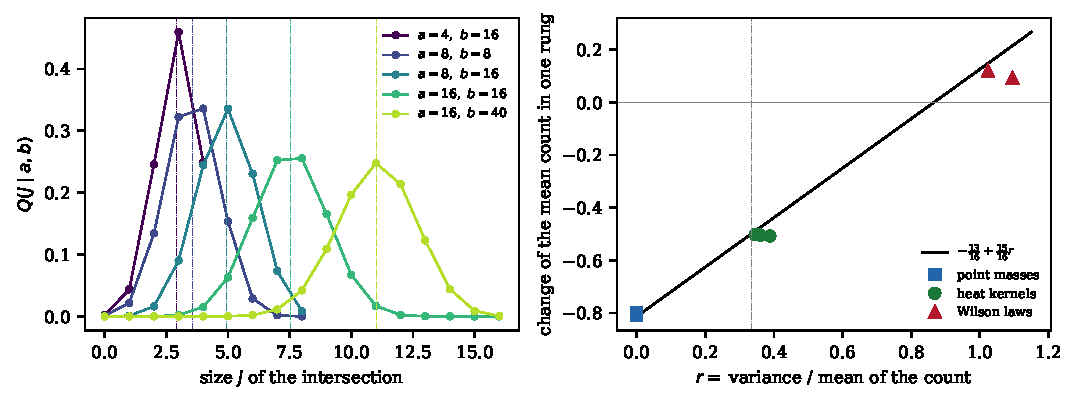
\includegraphics[width=\textwidth]{figures/counts_urn.pdf}
\caption[The hypergeometric kernel and the drift law]{Left: the coalescence kernel $Q(j\mid a,b)$, the hypergeometric law of the intersection of two random subsets of sizes $a$ and $b$ in a set of size $a+b+2$; dotted lines mark the means $ab/(a+b+2)$. Right: the change of the mean count over one exact rung against the ratio $r$ of variance to mean, for point masses, heat kernels and Wilson laws, with the line $-\frac{13}{16}+\frac{15}{16}r$; the vertical line is the fixed ratio $\frac13$.}
\label{fig:countsurn}
\end{figure}

The three numbers that had no explanation, a drift of $-0.81$ from a point mass, $-0.51$ from a heat kernel and $+0.11$ from a Wilson law, are $-\frac{13}{16}$, $-\frac12$ and $+\frac18$ (the first and third are proved in Theorem~\ref{thm:firstrung}, the second is not), the values of one linear function at $r=0$, $\frac13$ and $1$; the residual differences in Table~\ref{tab:drift} are the corrections of order $1/m$. A Wilson law has a Poisson count, with $r=1$, which is above the threshold $r=\frac{13}{15}$ at which the drift changes sign. That is why it gains order at its first rung. After one rung its ratio is $\frac38$ and its drift $-0.46$, after two $\frac13$ to within one percent. So the transient of Table~\ref{tab:notmonotone} (in Section~\ref{ch:kingman} below) lasts one rung, and the invariant class we were looking for is, to this order, a neighbourhood of the ray $r=\frac13$. The derivation is an asymptotic calculation and not a theorem; the kernel it rests on is exact.

\section{Consequences}

\begin{corollary}[the family $\mathcal M$ is closed]\label{cor:Mclosed}
Let $\mathcal M$ be the set of densities $\sum_j\pi(j)f_j$ with $\pi$ a probability law on the nonnegative integers. Then $\mathcal M$ contains every SU(2) heat kernel and every Wilson law, and is closed under products followed by normalisation and under convolution. Hence every rung of the exact Migdal Kadanoff ladder started from a heat kernel or a Wilson law, for any integer scale factor and any dimension, lies in $\mathcal M$. (Products are taken of bounded densities, so that the normalisation is finite; heat kernels and Wilson laws are bounded, and bounded densities stay bounded under products and convolutions.)
\end{corollary}

\begin{proof}
The Wilson law has density proportional to $e^{\kappa x}=e^{-\kappa}\sum_{m\ge0}\kappa^m(1+x)^m/m!$, a series of positive multiples of $f_m=2^mC_{m+1}^{-1}(1+x)^m$, so it lies in $\mathcal M$. The heat kernel lies in $\mathcal M$ by Theorem~\ref{thm:kingman}(ii), whose proof uses only Lemma~\ref{lem:fjchar}. For products, $f_af_b=\big(2^{a+b}/C_{a+1}C_{b+1}\big)(1+x)^{a+b}$ is a positive multiple of $f_{a+b}$, so if $\rho=\sum_a\pi(a)f_a$ and $\sigma=\sum_b\pi'(b)f_b$ then $\rho\sigma=\sum_{a,b}\pi(a)\pi'(b)\,c_{ab}f_{a+b}$ with $c_{ab}>0$ (all terms are nonnegative, so the double series may be rearranged); when $\rho\sigma$ is integrable, its normalisation is a probability density of the same form (and $\int\rho\sigma>0$, since every $f_j$ is positive off the antipode). For convolution, Theorem~\ref{thm:coalescence} and the same rearrangement give $\rho*\sigma=\sum_{a,b}\pi(a)\pi'(b)\sum_jQ(j\mid a,b)f_j=\sum_j\pi''(j)f_j$ with $\pi''(j)=\sum_{a,b}\pi(a)\pi'(b)Q(j\mid a,b)\ge0$, and $\sum_j\pi''(j)=1$ because each $Q(\cdot\mid a,b)$ is a probability law. Finally one rung with integer scale factor $\ell$ in dimension $d$ is the normalised power $\rho^{\ell^{d-2}}$ (bond moving) followed by the $\ell^2$ fold convolution (decimation), which are repeated products and convolutions with integer multiplicities; bounded densities stay bounded, as $\|\rho*\sigma\|_\infty\le\|\rho\|_\infty$.
\end{proof}

So at every rung of the exact ladder the density of a link is an absolutely monotone function of $1+\cos\theta$: all of its derivatives in $\cos\theta$ are nonnegative. In particular it is increasing and convex in $\cos\theta$, its character coefficients are positive, and it is a mixture of functions of positive type. None of this was known to us for the exact ladder before; the projection onto heat kernels had hidden it.

\begin{corollary}[the mean count is an observable]\label{cor:meancount}
For $\rho=\sum_j\pi(j)f_j$ in $\mathcal M$,
\[
\sum_jj\,\pi(j)=\Big\langle\frac1{1-\cos\theta}\Big\rangle_\rho-2=2\sum_{n\ge1}n\,u_n(\rho)-2 .
\]
For the heat kernel this is $2\sum_nn\,e^{-(n^2-1)t/4}-2=2\beta-\frac76+O(1/\beta)$.
\end{corollary}

\begin{proof}
The first equality is Proposition~\ref{prop:observable}, whose proof is by linearity from $\rho=f_j$, together with $\int\chi_n(1-\cos\theta)^{-1}=2$. For the heat kernel, $u_n=e^{-(n^2-1)t/4}$ with $t=2/\beta$, and the first Euler Maclaurin sum in the proof of Theorem~\ref{thm:harmonic} with $H_1=t/4=1/(2\beta)$ gives $2e^{H_1}\big(\frac1{2H_1}-\frac1{12}\big)-2=2\beta-\frac76+O(1/\beta)$.
\end{proof}

\paragraph{\normalfont\scshape The two operations.} Let $\nu_0$ be the law of $M_0$ in $\rho\propto\E[(1+x)^{M_0}]$, so that $\pi(j)\propto\nu_0(j)\,C_{j+1}2^{-j}$. Then bond moving with power $k$ and one convolution of decimation act by
\[
\nu_0\ \longmapsto\ \nu_0^{*k}\qquad\text{and}\qquad\pi\ \longmapsto\ \sum_{a,b}\pi(a)\,\pi(b)\,Q(\cdot\mid a,b),
\]
the first being the law of the sum of $k$ independent counts. The first multiplies the mean of $M_0$ by $k$. The second sends two counts $a$ and $b$ to a count of mean $ab/(a+b+2)$, which is less than the flat value $ab/(a+b)$ and less than $\min(a,b)$. A population is multiplied, then thinned in pairs. In flat space the thinning would exactly undo the multiplication in four dimensions; the $2$ in the denominator is what is left over, and it is the curvature of the group once more.

\paragraph{\normalfont\scshape Random walks.} By Lemma~\ref{lem:fjchar} the theorem is a statement about simple random walk: the pointwise product of the endpoint laws of two walks of $2\bar a$ and $2\bar b$ steps, restricted to $n\ge1$, is a positive combination of the endpoint laws of walks of $2J$ steps with $J\le\min(\bar a,\bar b)$. Two walks conditioned to end together look, at their common endpoint, like one shorter walk of random length. We have not found this statement in the literature; it may well be there.

\paragraph{\normalfont\scshape A worked case.} Take $a=b=2$, so $\bar a=\bar b=3$. The nodes are $s=9,4,1$ and $w_3(n^2)=1/\big((3-n)!\,(3+n)!\big)$ gives $w_3(9)=\frac1{720}$, $w_3(4)=\frac1{120}$, $w_3(1)=\frac1{48}$. The divided differences are
\[
w_3[9]=\tfrac1{720},\qquad w_3[9,4]=-\tfrac1{720},\qquad w_3[9,4,1]=\tfrac1{2880},
\]
alternating in sign as Lemma~\ref{lem:cm} requires, so $\omega_3=\frac1{720}$, $\omega_2=\frac1{720}$, $\omega_1=\frac1{2880}$. Multiplying by $(2!\,4!)^2/\big((J-1)!\,(J+1)!\big)$, which is $48$, $384$ and $1152$ for $J=3,2,1$, gives $Q(2)=\frac1{15}$, $Q(1)=\frac8{15}$, $Q(0)=\frac25$, with mean $\frac23=\frac{2\cdot2}{2+2+2}$.

\section{The exact ladder, looked at}

With the theorem in hand the exact ladder can be run on counts with no quadrature on the group: add four independent copies of $M_0$, reweight, and apply the coalescence twice. Starting from heat kernels at $\beta=2$, $3$ and $4$, with $k=4$ and $\ell^2=4$, where $\ell=2$ is the Migdal Kadanoff scale factor, written $b$ in Chapter~\ref{ch:strong}, in Table~\ref{tab:rungs}:

\begin{table}[t]
\centering\footnotesize
\begin{tabular}{lcccccccc}
\toprule
rung & 0 & 1 & 2 & 3 & 4 & 5 & 6 & 7 \\ \midrule
count, $\beta=4$ & 6.874 & 6.366 & 5.860 & 5.352 & 4.845 & 4.337 & 3.829 & 3.321 \\
$u_2$, $\beta=4$ & 0.687 & 0.670 & 0.651 & 0.629 & 0.604 & 0.576 & 0.544 & 0.507 \\
count, $\beta=3$ & 4.888 & 4.379 & 3.871 & 3.363 & 2.854 & & & \\
count, $\beta=2$ & 2.916 & 2.407 & 1.899 & 1.394 & 0.896 & & & \\
\bottomrule
\end{tabular}
\caption[The exact ladder on counts, by rung]{The mean count and the fundamental coefficient $u_2$ at each rung of the exact ladder ($k=4$, $\ell^2=4$), labelled by the starting heat kernel coupling $\beta$.}
\label{tab:rungs}
\end{table}

\begin{figure}[t]
\centering
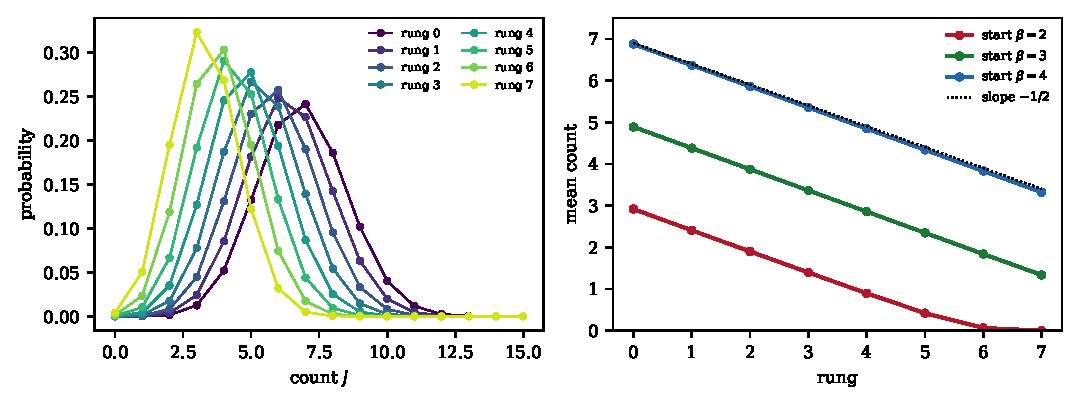
\includegraphics[width=\textwidth]{figures/counts.pdf}
\caption[The exact ladder on counts]{The exact Migdal Kadanoff ladder for SU(2), $\ell=2$ in four dimensions, as a process on integer counts. Left: the law of the count at eight successive rungs, started from the heat kernel at $\beta=4$. Right: the mean count against the rung from three starting couplings, with a line of slope $-\frac12$.}
\label{fig:counts}
\end{figure}

Three observations, the first two numerical and the third now partly a theorem.

The mean count falls by very nearly one half at each rung: $0.508$, $0.506$, $0.508$, $0.507$, $0.508$, $0.508$, $0.508$ from $\beta=4$, and the same from the other starts until the count is of order one (Figure~\ref{fig:counts}). In the count the exact ladder is a walk with constant drift. Since the mean count is $2\beta-\frac76$ to leading order, this is the decrement $\frac14$ of Theorem~\ref{thm:expansion}, now seen for the exact ladder and holding far outside weak coupling. The observable that falls linearly is $\langle1/(1-\cos\theta)\rangle$.

Along the computed heat kernel orbits the law of the count at each rung is below the law at the previous rung in the likelihood ratio order, and the law $\nu_0$ is log concave at every rung. So the exact ladder is monotone along these orbits in the strongest order available, and $u_2=\E[j/(j+3)]$ decreases.

The kernel $Q(j\mid a,b)$ is totally positive of order two in $(j,a)$ for each fixed $b$, and stochastically increasing in $a$, for all $a,b\le20$, in exact arithmetic (the total positivity is Corollary~\ref{cor:hypergeometric}(ii)). It is not totally positive in $(a,b)$ for fixed $j$, and should not be: the two parents compete.

\section{The harmonic law}\label{sec:harmonic}\index{harmonic law}

The drift law of Section~\ref{sec:hypergeometric} was obtained by the delta method. For decimation it can be made a theorem, because the mean count is linear in the law and the characters of the $f_j$ are explicit. Write $J=j+1$, so that $u_n(J)=\prod_{i=1}^{n-1}(J-i)/(J+1+i)$, and for $J_1,\dots,J_p$ put
\[
H_1=\sum_i\frac1{J_i},\qquad H_2=\sum_i\frac1{J_i^2},\qquad H_3=\sum_i\frac1{J_i^3}.
\]

\begin{theorem}[the harmonic law]\label{thm:harmonic}
Fix $p\ge2$ and $\lambda\ge1$. For $J_1,\dots,J_p$ with $\max J_i\le\lambda\min J_i$, the mean count of $f_{J_1-1}*\cdots*f_{J_p-1}$ is
\[
\frac1{H_1}-\frac76+\frac{H_2}{2H_1^2}-\frac{H_3}{3H_1^3}+R,\qquad |R|\le\frac{c(p,\lambda)}{\min J_i}.
\]
\end{theorem}

\begin{proof}
The mean count of a law with character coefficients $u_n$ is $2\sum_nn\,u_n-2$, and those of the convolution are $\prod_iu_n(J_i)$. Three facts about $u_n(J)$ are needed. First, since $\log(1-x)\le-x$ and $\log(1+y)\ge y/2$ for $0\le y\le1$, and $u_n(J)=0$ for $n>J$,
\[
u_n(J)\le\exp\Big(-\sum_{i=1}^{n-1}\frac{2i+1}{2J}\Big)=e^{-(n^2-1)/(2J)}.
\]
Second, expanding the logarithms to third order and summing over $i$,
\[
\log u_n(J)=-\frac{n^2-1}{J}+\frac{n^2-1}{2J^2}-\frac{n^4}{6J^3}+O\Big(\frac{n^2}{J^3}+\frac{n^4}{J^4}+\frac{n^6}{J^5}\Big),
\]
uniformly for $n\le J^{3/5}$. Third, by the Euler Maclaurin formula, as $H_1\to0$,
\[
\sum_{n\ge1}n\,e^{-H_1n^2}=\frac1{2H_1}-\frac1{12}+O(H_1),\qquad \sum_{n\ge1}n^3e^{-H_1n^2}=\frac1{2H_1^2}+O(1),
\]
\[
\sum_{n\ge1}n^5e^{-H_1n^2}=\frac1{H_1^3}+O(1).
\]
By the first fact the terms with $n>J^{3/5}$ contribute less than any power of $1/J$. For the others the second fact gives
\[
\prod_iu_n(J_i)=e^{H_1}e^{-H_1n^2}\Big(1+\frac{H_2n^2}{2}-\frac{H_3n^4}{6}+\varepsilon_n\Big),
\]
where $\sum_nn\,e^{-H_1n^2}|\varepsilon_n|=O(1/\min J_i)$, because each term of $\varepsilon_n$ is of relative order $J^{-2}$ when $n$ is of order $\sqrt J$ and the leading sum is of order $J$. The third fact then gives
\[
\sum_nn\prod_iu_n(J_i)=\Big(1+H_1\Big)\Big(\frac1{2H_1}-\frac1{12}\Big)+\frac{H_2}{4H_1^2}-\frac{H_3}{6H_1^3}+O\Big(\frac1{\min J_i}\Big),
\]
and doubling and subtracting $2$ gives the statement.
\end{proof}

The leading term is the harmonic sum: counts compose under decimation as resistances in parallel, or as $J=2\beta$ composes for heat kernels, where $1/J$ is proportional to time and times add. The constant $-\frac76$ is the one in Corollary~\ref{cor:meancount}. For $p=2$ the theorem can be compared with the exact mean $ab/(a+b+2)=1/H_1-1+1/(J_1+J_2)$: the three constants of the theorem sum to $-1$ for every ratio $J_1/J_2$, as they should.

\begin{corollary}[the drift from a point mass]\label{cor:pointdrift}
The exact rung with $k$ copies and $p$ fold convolution takes $f_m$ to a law with mean count
\[
\frac{km}{p}+c_p+O\Big(\frac1m\Big),\qquad c_p=\frac{3}{2p}-\frac76-\frac1{3p^2}.
\]
For $k=p=4$ the drift is $c_4=-\frac{13}{16}$, and for $k=p=2$ it is $c_2=-\frac12$.
\end{corollary}

\begin{proof}
Bond moving takes $f_m$ to $f_{km}$ exactly. Put $J_i=km+1$ in the theorem: $1/H_1=(km+1)/p$, $H_2/2H_1^2=1/2p$ and $H_3/3H_1^3=1/3p^2$.
\end{proof}

So the first of the three unexplained numbers is a theorem. In rational arithmetic the drift from $f_m$ at $k=p=4$ is $-0.79759$, $-0.80875$ and $-0.81156$ at $m=20$, $80$ and $320$, approaching $-\frac{13}{16}$ at the rate $0.30/m$. As $p\to\infty$ the constant $c_p$ tends to $-\frac76$: a long convolution of point masses is a heat kernel, and its mean count is $2\beta-\frac76$.

\begin{corollary}[decimation of a concentrated law]\label{cor:decdrift}
Let $\pi_M$ be laws on the counts with mean $M\to\infty$, variance $vM+o(M)$ and $E|a-M|^3=O(M^{3/2})$. Then the $p$ fold convolution of $\sum_a\pi_M(a)f_a$ with itself has mean count
\[
\frac Mp+c_p-\frac{(p-1)\,v}{p^2}+o(1).
\]
\end{corollary}

\begin{proof}
The mean count is the expectation of the function of Theorem~\ref{thm:harmonic} over independent $a_1,\dots,a_p$ from $\pi_M$. The event that some $a_i$ lies outside $[M/2,2M]$ has probability $O(M^{-3/2})$ and the mean count never exceeds $\min a_i$, so that event contributes $o(1)$. On its complement expand $1/H_1$ to second order about $J_i=M+1$: the pure second derivatives are $-2(p-1)/(p^3M)$, the mixed ones have expectation zero, and the third derivatives are $O(M^{-2})$ against third moments $O(M^{3/2})$. The terms in $H_2$ and $H_3$ are continuous and take their values at the centre.
\end{proof}

At $p=4$ the correction is $-\frac3{16}v$, which is what two coalescences gave in Section~\ref{sec:hypergeometric}.

\section{The count as an observable, and the first rung}\label{sec:observable}\index{mean count!as an observable}

The other half of a rung is bond moving, and for it a different description of the mean count is the useful one.

\begin{proposition}[the count is an observable]\label{prop:observable}
For every $\rho=\sum_j\pi(j)f_j$ in $\mathcal M$ with finite mean count,
\[
\sum_jj\,\pi(j)=E_\rho\Big[\frac{1}{1-\cos\theta}\Big]-2=E_\rho\Big[\frac1{2\sin^2(\theta/2)}\Big]-2 .
\]
\end{proposition}

\begin{proof}
Both sides are linear in $\rho$, so take $\rho=f_j$. Under $f_j$ the variable $y=\cos^2(\theta/2)$ has the $\mathrm{Beta}(j+\frac32,\frac32)$ law, and $1-\cos\theta=2(1-y)$. For a $\mathrm{Beta}(a,b)$ variable $E[1/(1-y)]=(a+b-1)/(b-1)$, which here is $2(j+2)$; half of it, less $2$, is $j$.
\end{proof}

The function $2\sin^2(\theta/2)$ is the one of the lemma of Section~\ref{ch:routeB}, met here on the group. The proposition says that the latent count, which was introduced as a mixing variable, has a mean that can be measured on a configuration: it is the expectation of the reciprocal of the Wilson action density, less two. The singularity at the identity is integrable against Haar measure, which vanishes there like $\theta^2$. It also gives the count of a law in closed form to the order needed. For $\rho=c\prod_m(1+x/\gamma_m)$ in the class $\mathcal L$ of Chapter~\ref{ch:zeros}, the densities $c\prod_m(1+x/\gamma_m)$ with $\gamma_m\ge1$ and $\sum_m1/\gamma_m<\infty$ together with their locally uniform limits, put
\[
\Sigma_1=\sum_m\frac1{\gamma_m+1},\qquad \Sigma_2=\sum_m\frac1{(\gamma_m+1)^2},\qquad r=1-\frac{2\Sigma_2}{\Sigma_1},
\]
so that $\Sigma_1$ and $-\Sigma_2$ are the first two derivatives of $\log\rho$ in $x$ at the identity, and $0\le r<1$.

\begin{lemma}[count of a law with real zeros]\label{lem:Lcount}
For $\rho\in\mathcal L$ the count law $\pi$ has, as $\Sigma_1\to\infty$ and uniformly in the zeros,
\[
\text{mean}=2\Sigma_1-\frac32\,r+O(\Sigma_1^{-1/2}),\qquad \text{variance}=2\Sigma_1\,r+O(\Sigma_1^{1/2}),
\]
\[
E_\pi|j-2\Sigma_1|^3=O(\Sigma_1^{3/2}).
\]
\end{lemma}

\begin{proof}
Writing $1+x/\gamma=\big((\gamma-1)+(1+x)\big)/\gamma$ shows that the unnormalised weights are those of a sum of independent Bernoulli variables with parameters $1/\gamma_m$, and $\pi(j)\propto\nu_0(j)\,C_{j+1}/2^j$. Put $C_{j+1}/2^j=2^j\varphi(j)$. The factor $2^j$ is an exponential tilt and turns the parameters into $q_m=2/(\gamma_m+1)$; so $\pi(j)\propto P(N=j)\,\varphi(j)$ with $N$ a sum of independent Bernoulli($q_m$) variables, of mean $\mu=2\Sigma_1$ and variance $\sigma^2=2\Sigma_1-4\Sigma_2=\mu r$. The factor $\varphi(j)=C_{j+1}/4^j$ has $\varphi(j+1)/\varphi(j)=1-3/(2j+6)$, so on $[\mu/2,2\mu]$ it is $\varphi(\mu)\big(1-\frac32(j-\mu)/\mu+O((j-\mu)^2/\mu^2)\big)$, and $N$ leaves that interval with probability exponentially small in $\mu$ by Bernstein's inequality. Hence $E_\pi g=E[g(N)\varphi(N)]/E[\varphi(N)]$ gives the mean $\mu-\frac32\sigma^2/\mu$ with error $O(E|N-\mu|^3/\mu^2+1/\mu)$, and the second and third moments about $\mu$ are those of $N$ up to a factor $1+O(\mu^{-1/2})$; for a sum of independent Bernoulli variables $E|N-\mu|^3=O(\sigma^3+\sigma)$.
\end{proof}

Laplace's method applied to Proposition~\ref{prop:observable} gives the same mean in the sharper form $2\Sigma_1-\frac32+3\Sigma_2/\Sigma_1+O(1/\Sigma_1)$, which is exact for $f_j$, is $2\kappa-\frac32$ for the Wilson law, and is $2\beta-\frac76$ for the heat kernel, where $\Sigma_1=\beta-\frac13$ and $\Sigma_2=\frac13\beta$ to leading order (by Laplace's method from the small time expansion of $\log K_t$, not proved here). So the ratio $r$ of variance to mean is $0$ for a point mass, $1$ for a Wilson law and $\frac13$ for a heat kernel at weak coupling, and it is read off from two derivatives of the action at the identity.

\begin{theorem}[the first rung]\label{thm:firstrung}
Let $\rho\in\mathcal L$. One exact rung of the ladder, $k=4$ copies and fourfold convolution, changes the mean count by
\[
-\frac{13}{16}+\frac{15}{16}\,r+o(1)\qquad\text{as }\Sigma_1\to\infty .
\]
In particular the change tends to $-\frac{13}{16}$ from point masses and to $+\frac18$ from Wilson laws as $\kappa\to\infty$.
\end{theorem}

\begin{proof}
Bond moving takes $\rho$ to $\rho^4$, which is in $\mathcal L$ with $\Sigma_1$ and $\Sigma_2$ multiplied by $4$ and $r$ unchanged. By Lemma~\ref{lem:Lcount} its count law has mean $4\cdot2\Sigma_1-\frac32r+o(1)$, which is $4M+\frac92r+o(1)$ with $M$ the mean count of $\rho$, variance $r$ times its mean to leading order, and third moment of the order required by Corollary~\ref{cor:decdrift}. That corollary with $p=4$ and $v=r$ gives the mean after decimation. Since $r$ lies in $[0,1]$ and may vary along the family, apply it by subsequences: from any sequence with $\Sigma_1\to\infty$ extract a subsequence along which $r$ converges to some $v$; on it the corollary applies with that fixed $v$ and gives $-\frac{13}{16}+\frac{15}{16}v+o(1)=-\frac{13}{16}+\frac{15}{16}r+o(1)$ for the change of the mean. Every subsequence has a further subsequence on which the formula holds, so it holds along the whole family. With $v=r$ the mean after decimation is,
\[
\frac{4M+\frac92r}{4}+c_4-\frac{3}{16}\,r+o(1)=M-\frac{13}{16}+\frac{15}{16}\,r+o(1).
\]
The Wilson law is a limit of members of $\mathcal L$ and its count law is the Poisson case of the lemma, with $r=1$.
\end{proof}

\paragraph{\normalfont\scshape The heat kernel.} The heat kernel belongs to $\mathcal L$ (Theorem~\ref{thm:product} of Chapter~\ref{ch:progress}), so the theorem applies to it, and with $r\to\frac13$ it would give $-\frac12$ as $\beta\to\infty$. We have not proved that. The value $r\to\frac13$ rests on $\Sigma_1=\beta-\frac13$ and $\Sigma_2=\frac13\beta$ to leading order, which we obtained from the small time expansion $\log K_t\approx-\beta\theta^2/2+\log(\theta/\sin\theta)$ by Laplace's method, without an error bound. So $-\frac12$ from heat kernels is a numerical observation with an asymptotic derivation (the exact rungs from heat kernels in the table of Section~\ref{sec:hypergeometric} approach it, $-0.507$ at $\beta=4$ and $-0.502$ at $\beta=16$), not a theorem. To prove it, it is enough to show $\Sigma_1=\beta+O(1)$ and $\Sigma_2=\frac13\beta+o(\beta)$ for $\Sigma_i=\sum_m\gamma_m(t)^{-i}$ with $t=2/\beta$.

\begin{figure}[t]
\centering
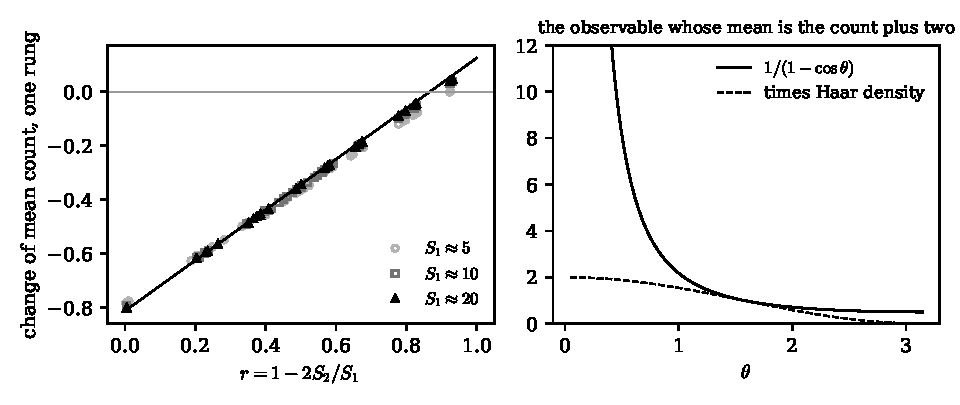
\includegraphics[width=\textwidth]{figures/firstrung.pdf}
\caption[The first rung theorem]{Left: the exact change of the mean count over one rung for $180$ random laws of the class $\mathcal L$ of three sizes, against the line $-\frac{13}{16}+\frac{15}{16}r$ of Theorem~\ref{thm:firstrung}. Right: the observable $1/(1-\cos\theta)$ of Proposition~\ref{prop:observable}, and its product with the Haar density, which is $1+\cos\theta$.}
\label{fig:firstrung}
\end{figure}

\paragraph{\normalfont\scshape On the lattice.} Proposition~\ref{prop:observable} makes sense for any law of a plaquette variable, whether or not it lies in $\mathcal M$: define the count of a lattice measure as $E[1/(1-\frac12\operatorname{tr}U_p)]-2$. It is finite on any finite lattice, since the density of a plaquette at the identity is bounded, it is $2\beta-\frac76$ for heat kernel plaquettes and $2\kappa-\frac32$ for Wilson plaquettes at weak coupling in two dimensions, where the plaquettes are independent, and it is zero for Haar measure. It is a candidate for the quantity to follow under blocking on $\mathbb Z^4$, in place of the coupling, with the advantage that it is defined without reference to an action. The next section computes it on a four dimensional lattice.

So two of the three numbers are theorems, for the first rung, and the third, $-\frac12$ from heat kernels, is a theorem once $r\to\frac13$ is proved. The proof does not go beyond it, because decimation is not known to keep a law in $\mathcal L$: that is Conjecture~\ref{conj:Lclosed}. If the conjecture holds, the theorem applies at every rung for as long as the count is large; if in addition the variance recursion of Section~\ref{sec:hypergeometric}, which is a leading order derivation, holds with a remainder, the ratio follows $r'=\frac5{16}+\frac1{16}r$ to its fixed point $\frac13$, and the drift settles at $-\frac12$ per rung from any start in $\mathcal L$; that is the constant drift seen in the exact ladder above and the reason the Wilson law, after one rung of gain, loses count like a heat kernel. Table~\ref{tab:firstrung} compares the theorem with exact rungs.

\begin{table}[t]
\centering\small
\begin{tabular}{lcccc}
\toprule
law in $\mathcal L$ & count & $r$ & exact & theorem \\ \midrule
$40$ zeros at $\gamma=1$ & $40.00$ & $0$ & $-0.805$ & $-0.813$ \\
$60$ zeros at $\gamma=2$ & $39.51$ & $0.333$ & $-0.499$ & $-0.500$ \\
$80$ random zeros drawn uniformly from $[1,6]$ & $38.08$ & $0.457$ & $-0.388$ & $-0.384$ \\
$120$ zeros at $\gamma=5$ & $39.01$ & $0.667$ & $-0.193$ & $-0.188$ \\
$300$ zeros at $\gamma=20$ & $27.24$ & $0.905$ & $+0.021$ & $+0.036$ \\
\bottomrule
\end{tabular}
\caption[The first rung against the theorem]{The change of the mean count over one exact rung from laws of the class $\mathcal L$, against $-\frac{13}{16}+\frac{15}{16}r$. The mean count agrees with $E[1/(1-\cos\theta)]-2$ computed by quadrature to all digits shown.}
\label{tab:firstrung}
\end{table}

\section{The count on a four dimensional lattice}\label{sec:countlattice}\index{mean count!on the lattice}\index{link integration}

The plain average of $1/(1-\frac12\operatorname{tr}U_p)$ over a simulation has a finite mean and an infinite variance, because the density of a plaquette at the identity is positive and the Haar weight vanishes there only like $\theta^2$. One link integration removes the difficulty.

\begin{proposition}[an estimator with finite variance]\label{prop:linkint}
Let $W$ be a random element of SU(2) with class density $\sum_nn\,u_n\chi_n$, where $\sum_nn\,u_n<\infty$, and $Y$ a fixed element. Then
\[
E\Big[\frac{1}{1-\frac12\operatorname{tr}(WY)}\Big]=2\sum_{n\ge1}u_n\,\chi_n(Y).
\]
In a lattice gauge theory with Wilson action, a link given all the others is $WV^{-1}$ with $V$ the normalised sum of its staples and $u_n=I_n(\kappa)/I_1(\kappa)$, $\kappa=\beta|{\rm staples}|$ with $|{\rm staples}|$ the norm of the staple sum. So for any loop that passes once through the link, with $R$ the rest of the loop, the count of the loop is the average of $2\sum_n\big(I_n(\kappa)/I_1(\kappa)\big)\chi_n(V^{-1}R)-2$, a bounded function of the configuration.
\end{proposition}

\begin{proof}
$\int\chi_n/(1-\cos\theta)$ against Haar measure is $\frac2\pi\int_0^\pi\chi_n(\theta)(1+\cos\theta)\,d\theta=2$ for every $n$, so $1/(1-\cos\theta)=2\sum_n\chi_n$ as a distribution on class functions, and $E\,\chi_n(WY)=u_n\chi_n(Y)$ for a conjugation invariant $W$.
\end{proof}

We ran it on an $8^4$ lattice, forty configurations at each coupling, for the plaquette and for the $2\times2$ loop. Beside each count we put the count of a Wilson law and of a heat kernel with the same fundamental coefficient $u_2=\langle\frac12\operatorname{tr}\rangle$: by Lemma~\ref{lem:Lcount} the two differ through the ratio $r$, so the comparison says which shape the lattice law has.

\begin{table}[t]
\centering\small
\begin{tabular}{rcccccc}
\toprule
 & \multicolumn{3}{c}{plaquette} & \multicolumn{3}{c}{$2\times2$ loop} \\
$\beta$ & count & Wilson & heat & count & Wilson & heat \\ \midrule
$1.5$ & $2.173(4)$ & $2.172$ & $1.901$ & $0.071(2)$ & $0.077$ & $0.075$ \\
$2.0$ & $3.666(6)$ & $3.686$ & $3.252$ & $0.302(3)$ & $0.316$ & $0.299$ \\
$2.3$ & $5.234(11)$ & $5.348$ & $4.809$ & $0.794(6)$ & $0.866$ & $0.781$ \\
$2.5$ & $6.299(11)$ & $6.477$ & $5.896$ & $1.227(6)$ & $1.364$ & $1.207$ \\
$2.7$ & $7.193(7)$ & $7.403$ & $6.801$ & $1.557(4)$ & $1.756$ & $1.542$ \\
$3.0$ & $8.496(13)$ & $8.731$ & $8.108$ & $2.038(7)$ & $2.312$ & $2.023$ \\
$4.0$ & $12.636(11)$ & $12.915$ & $12.267$ & $3.567(8)$ & $4.004$ & $3.545$ \\
\bottomrule
\end{tabular}
\caption[The count on an $8^4$ lattice]{The count $E[1/(1-\frac12\operatorname{tr}U)]-2$ of the plaquette and of the $2\times2$ loop in SU(2) lattice gauge theory on $8^4$, by the estimator of Proposition~\ref{prop:linkint}, with the counts of the Wilson law and of the heat kernel having the same $\langle\frac12\operatorname{tr}U\rangle$. Errors are standard errors over forty configurations and ignore autocorrelation.}
\label{tab:countlattice}
\end{table}

Two things can be read from Table~\ref{tab:countlattice}. The plaquette of the four dimensional theory has, at strong coupling, the count of a Wilson law to the accuracy measured, and moves a third of the way toward the heat kernel by $\beta=2.5$: the interaction with its neighbours gives the one plaquette law some of the curvature that the Wilson action lacks. And the $2\times2$ loop has the count of a heat kernel to within two per cent from $\beta=2$ on, and not that of a Wilson law, from which it differs by five to twelve per cent: a holonomy that is a product of several fluctuating pieces has the shape of a heat kernel. This is what the ladder does to a Wilson law in one decimation, and what the first rung theorem measures through $r$; here it is seen in the full theory.

\begin{figure}[t]
\centering
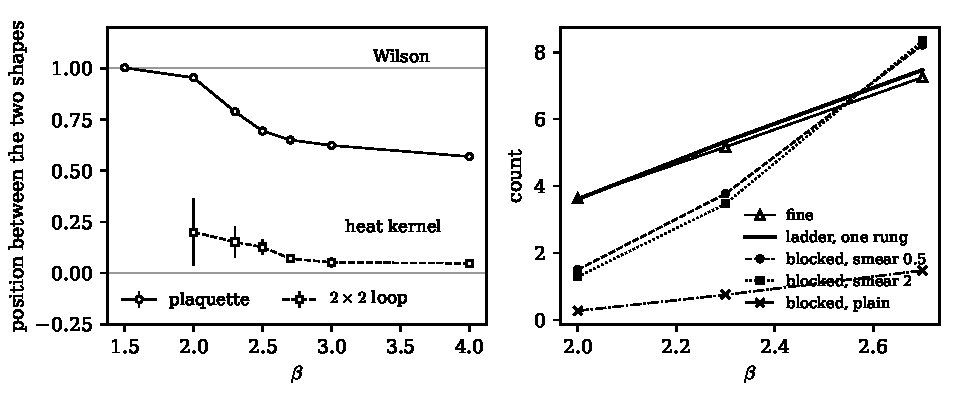
\includegraphics[width=\textwidth]{figures/count_lattice.pdf}
\caption[Shapes and counts on the lattice]{Left: the position of the measured count between that of the heat kernel, at $0$, and that of the Wilson law, at $1$, with the same $u_2$, for the plaquette and the $2\times2$ loop on $8^4$. Right: the count of the fine plaquette, of one rung of the ladder, and of the blocked plaquette for three blockings.}
\label{fig:countlattice}
\end{figure}

For a blocked lattice no link can be integrated out once the blocked links are smeared, and we took the count from the characters, $2\sum_{n\le40}E\chi_n-2$, each term of which has finite variance; on the unblocked lattice this agrees with the table to about two standard errors. Table~\ref{tab:countblocked} sets the count of the blocked plaquette, for two amounts of smearing, beside one exact rung of the ladder started from the Wilson law matched to the fine plaquette.

\begin{table}[t]
\centering\small
\begin{tabular}{rccccc}
\toprule
$\beta$ & fine & ladder & blocked, plain & smear $0.5$ & smear $2$ \\ \midrule
$2.0$ & $3.64(2)$ & $3.61$ & $0.27(4)$ & $1.50(3)$ & $1.29(7)$ \\
$2.3$ & $5.17(3)$ & $5.33$ & $0.75(6)$ & $3.77(9)$ & $3.47(12)$ \\
$2.7$ & $7.25(8)$ & $7.47$ & $1.48(3)$ & $8.22(11)$ & $8.34(23)$ \\
\bottomrule
\end{tabular}
\caption[The count under blocking, lattice against ladder]{The count of the plaquette on $8^4$, the count after one exact rung of the ladder from the matched Wilson law, and the count of the plaquette of the lattice blocked to $4^4$ with scale factor two: blocked links without smearing, and with the staples added with weight $0.5$ and $2$ before projection.}
\label{tab:countblocked}
\end{table}

At $\beta=2.0$ and $2.3$ the blocked lattice has a smaller count than the ladder, for every smearing: the true flow loses order faster than the ladder does, which is the direction of the comparison asked for in Chapter~\ref{ch:sandwich}, since the count is the mean of an increasing function of $\cos\theta$. At $\beta=2.7$ the inequality is reversed for the smeared blockings. The smeared blocked plaquettes have the count of a Wilson law with their $u_2$, within errors, and the unsmeared ones are close to that of a heat kernel, so the shape of the blocked law depends on the blocking as much as its coupling does.

To see whether the reversal at $\beta=2.7$ is an effect of the small box we repeated the computation on $16^4$, with two blockings, to $8^4$ and to $4^4$, smearing $0.5$, thirty configurations at each coupling.

\begin{table}[t]
\centering\small
\begin{tabular}{rcccccc}
\toprule
 & \multicolumn{2}{c}{fine} & \multicolumn{2}{c}{blocked once} & \multicolumn{2}{c}{blocked twice} \\
$\beta$ & lattice & ladder & lattice & ladder & lattice & ladder \\ \midrule
$2.3$ & $5.23(1)$ & $5.34$ & $3.77(4)$ & $5.34$ & $1.27(8)$ & $4.87$ \\
$2.5$ & $6.31(1)$ & $6.48$ & $6.09(2)$ & $6.51$ & $4.04(16)$ & $6.04$ \\
$2.7$ & $7.22(1)$ & $7.43$ & $8.14(7)$ & $7.48$ & $6.75(17)$ & $7.01$ \\
\bottomrule
\end{tabular}
\caption[Two blockings on $16^4$]{The count of the plaquette on $16^4$ and after one and two blockings with scale factor two and smearing $0.5$, against the count after the same number of exact rungs of the ladder from the Wilson law matched to the fine plaquette.}
\label{tab:countblocked2}
\end{table}

The reversal is not an effect of the box: at $\beta=2.7$ the plaquette blocked once has a larger count than the fine one on $16^4$ also, $8.14$ against $7.22$, and exceeds the ladder. It is an effect of the smearing, which at weak coupling removes short distance fluctuations from the blocked link faster than a rung of the ladder does. After the second blocking the lattice is below the ladder at all three couplings, and at $\beta=2.3$ and $2.5$ it is below at both levels, by a margin that grows with the level. So the comparison holds where the coupling has begun to run and fails, for this blocking, at the first step from weak coupling: an inequality between the two flows has to be asked either with an error term or from the second step on, and it depends on the blocking. These are small lattices and a count that depends on the choice of blocked link; they are an illustration of how the observable behaves, not a measurement of the flow.

\paragraph{\normalfont\scshape Log concavity.} One half of Open problem~\ref{op:logconcave} has a short answer.

\begin{proposition}\label{prop:Llogconcave}
For every law of the class $\mathcal L$ the count law $\pi$ is log concave.
\end{proposition}

\begin{proof}
For a finite product the unnormalised weights $\nu_0$ are those of a sum of $N$ independent Bernoulli variables, so by Newton's inequalities $\nu_0(j)^2\ge(1+1/j)\,\nu_0(j-1)\,\nu_0(j+1)$. The count law is $\pi(j)\propto\nu_0(j)Z_j$ with $Z_j=C_{j+1}/2^j$, and from $C_{n+1}/C_n=2(2n+1)/(n+2)$,
\[
\frac{Z_{j+1}Z_{j-1}}{Z_j^2}=1+\frac{3}{2j^2+7j+3}\le1+\frac1j .
\]
Infinite products follow in the limit.
\end{proof}

For the other half, whether coalescence preserves log concavity, we have only evidence: in rational arithmetic, over $400$ random log concave $\nu_0$ and $400$ random log concave $\pi$ on up to fifteen points, one coalescence left the law log concave every time, with smallest ratios $\nu(j)^2/\nu(j-1)\nu(j+1)$ of $1.049$ and $1.223$.

\section{What is proved and what is left}

Proved:
\begin{itemize}
\item the exact ladder lives in $\mathcal M$; bond moving is addition of counts, and decimation is a coalescence with the hypergeometric kernel of Theorem~\ref{thm:hypergeometric}, which is totally positive of order two;
\item the mean count is the observable $E[1/(1-\cos\theta)]-2$ (Proposition~\ref{prop:observable}), with an estimator of finite variance on the lattice (Proposition~\ref{prop:linkint});
\item under convolution the mean count obeys the harmonic law with an error $O(1/J)$ (Theorem~\ref{thm:harmonic});
\item from any law with real zeros the first rung changes the mean count by $-\frac{13}{16}+\frac{15}{16}r+o(1)$ (Theorem~\ref{thm:firstrung});
\item every law with real zeros has a log concave count (Proposition~\ref{prop:Llogconcave}).
\end{itemize}

Not proved, and now sharply posed:

\begin{problem}\label{op:Qtp2}
Show that $Q(j\mid a,b)$ is totally positive of order two in $(j,a)$ for every $b$. (Solved: Corollary~\ref{cor:hypergeometric}.)
\end{problem}

\begin{problem}\label{op:logconcave}
Show that the exact ladder preserves log concavity of $\nu_0$. Sums of independent log concave counts are log concave; the question is the coalescence. (Proposition~\ref{prop:Llogconcave} shows that every law of the class $\mathcal L$ has a log concave count; exact computation supports the rest.)
\end{problem}

\begin{problem}\label{op:drift}
Explain the constant drift. (Answered to leading order in Section~\ref{sec:hypergeometric}: the drift is $-\frac{13}{16}+\frac{15}{16}r$ and $r\to\frac13$. Theorem~\ref{thm:firstrung} proves the drift formula for the first rung from any law of the class $\mathcal L$, but $r\to\frac13$ for heat kernels is not proved; later rungs wait on Conjecture~\ref{conj:Lclosed}.)
\end{problem}

These would be steps toward a contraction theorem for the exact ladder, but they are not sufficient and the target needs care. Section~\ref{ch:kingman} shows that the ladder is not monotone on all of $\mathcal M$, nor on all laws with log concave count, and that from a Wilson law with $\kappa\ge2$ the fundamental coefficient rises at the first rung. The theorem to aim for concerns the orbit of a heat kernel, or a class of laws that contains it and is preserved, and that class is not yet identified. What the count formulation does remove is the bad cap at the antipode: on the group every $f_j$ with $j\ge1$ vanishes there, and on the integers only the state $j=0$ charges it.

\section{The same theorem for the circle}

It is worth seeing how much of this is special to SU(2). On U(1) the analogous densities are $(1+\cos\theta)^j$ with respect to Lebesgue measure on the circle, with Fourier coefficients $\binom{2j}{j-n}/\binom{2j}{j}$: the walk again, now without the factor $(J+1)/J$ and with the node $n=0$ included. The proof of Theorem~\ref{thm:coalescence} goes through word for word with nodes $0,1,4,\dots,a^2$, since it used only the complete monotonicity of $w_N$. So the family of mixtures of $(1+\cos\theta)^j$ on the circle is closed under convolution with a positive kernel as well, and the Villain and Wilson laws of the abelian theory lie in it (for the Villain law this is the circle analogue of Theorem~\ref{thm:kingman}, with death rate $\frac12j^2$). What differs is the mean: on the circle the functional $\mathsf W$ is not available, and the abelian ladder has the exponentially small decrement found for U(1) in Chapter~\ref{ch:path}, not a constant one. The positivity is common to both groups; the drift of one half is the nonabelian curvature.

\section{Assessment}

This is the first statement in the book about the exact ladder that is a theorem at every coupling and uses no projection. It does not touch $\mathbb Z^4$. Its use for the real problem is indirect and we state it as a hope: the family $\mathcal M$ is defined on one link, and the Wilson measure on any lattice is a product of members of $\mathcal M$ over plaquettes; so the lattice measure has a representation by integer counts on plaquettes with positive weights before the links are integrated. Whether blocking on $\mathbb Z^4$ acts on those counts by a positive kernel, as it does on a hierarchical lattice, is the comparison problem of Chapter~\ref{ch:sandwich} in its most concrete form so far.

\section{Kingman's coalescent in the heat kernel}\label{ch:kingman}\index{Kingman, J. F. C.}\index{coalescent}\index{Wright Fisher diffusion}\index{Ewens sampling formula}\index{duality}

The count of the preceding sections was found by multiplying out a product. It has a name. In the variable $y=\cos^2(\theta/2)$ Brownian motion on SU(2) is a Wright Fisher diffusion, and the latent count is the number of ancestral lineages in Kingman's coalescent. The next sections prove that, draw three consequences, and then ask what else in Kingman's work, and in our book on statistical methods for genetics~\cite{Po26g}, bears on the gap. Of that book we use its contents; of Kingman, the papers of 1963, 1973 and 1982 \cite{Ki63,Ki73,Ki82}, and for the paintbox representation his paper of 1978.

\section{Brownian motion on SU(2) is a Wright Fisher diffusion}\label{sec:wf}

\begin{proposition}\label{prop:wf}
Let $y=\cos^2(\theta/2)=\frac12(1+\cos\theta)$. On class functions,
\[
\Delta=y(1-y)\,\partial_y^2+\big(\tfrac32-3y\big)\,\partial_y=2\,\mathcal G,
\]
where
\[
\mathcal G=\tfrac12y(1-y)\,\partial_y^2+\tfrac12\big(\theta_{\mathrm m,1}(1-y)-\theta_{\mathrm m,2}y\big)\partial_y,\qquad\theta_{\mathrm m,1}=\theta_{\mathrm m,2}=\tfrac32 .
\]
So the class angle of the Brownian motion with heat kernel $K_t$ is, in the variable $y$, the neutral two allele Wright Fisher diffusion with symmetric mutation and total mutation parameter $\theta_{\mathrm m}=3$, run for the time $\tau=t/2$ and started from fixation, $y=1$. Its stationary law is Beta with parameters $\frac32,\frac32$, which is Haar measure.
\end{proposition}

\begin{proof}
From $\Delta=\partial_\theta^2+2\cot\theta\,\partial_\theta$, $dy/d\theta=-\frac12\sin\theta$ and $\sin^2\theta=4y(1-y)$. The heat kernel has generator $\frac14\Delta=\frac12\mathcal G$.
\end{proof}

The identification is of the kind that Kac would have liked: the gene frequency of population genetics and the plaquette variable of gauge theory obey the same equation, with the dimension of the group, three, as the mutation rate.

\section{Duality: heat flow is the death of lineages}\label{sec:duality}

Let $A$ be the pure death process on the nonnegative integers that jumps from $m$ to $m-1$ at rate $\frac12m(m+2)$. For $\theta_{\mathrm m}=3$ this is the process counting the lineages of Kingman's coalescent in which each pair merges at rate one and each lineage is lost by mutation at rate $\theta_{\mathrm m}/2$: the rate is $\binom m2+\frac{3m}2=\frac12m(m+2)$. It comes down from infinity, and we write $P_\infty$ for its law started there.

\begin{theorem}[coalescent duality]\label{thm:kingman}
With $f_j\propto(1+\cos\theta)^j$ the densities of Theorem~\ref{thm:coalescence}:
\begin{enumerate}
\item[(i)] $f_a*K_s=\sum_{j\le a}P_a\big(A(s/2)=j\big)\,f_j$ for every $a\ge0$ and $s>0$;
\item[(ii)] $K_t=\sum_{j\ge0}P_\infty\big(A(t/2)=j\big)\,f_j$.
\end{enumerate}
The latent count of the heat kernel in Proposition~\ref{prop:latentcount} is the number of lineages of Kingman's coalescent with mutation, at time $t/2$.
\end{theorem}

\begin{proof}
By Lemma~\ref{lem:fjchar}, $f_j$ has coefficients $u_n(J)$ with $J=j+1$, and $u_n(J-1)/u_n(J)=(J^2-n^2)/(J^2-1)$. The death rate from $j$ is $\frac12j(j+2)=\frac12(J^2-1)$, so the generator $G$ of $A$ applied to $j\mapsto u_n(j+1)$ gives
\[
\tfrac12(J^2-1)\big[u_n(J-1)-u_n(J)\big]=-\tfrac12(n^2-1)\,u_n(J).
\]
Thus $j\mapsto u_n(j+1)$ is an eigenfunction of $G$ with eigenvalue $-\frac12(n^2-1)$, and $\E_a\big[u_n(A(\tau)+1)\big]=e^{-(n^2-1)\tau/2}u_n(a+1)$. With $\tau=s/2$ the right side is the $n$th coefficient of $f_a*K_s$, which is (i). As $a\to\infty$, $u_n(a+1)\to1$ for each $n$, $f_a$ tends to the unit mass at the identity, and (ii) follows.
\end{proof}

The proof is three lines because the work was done by Lemma~\ref{lem:fjchar}. In population genetics (ii) is the expansion of the transition density of the Wright Fisher diffusion in Beta laws weighted by the ancestral process, due to Griffiths~\cite{Gri80} and to Tavar\'e~\cite{Tav84}, and (i) is the statement that mixtures of Beta laws are preserved by the diffusion, with the death process moving the weights, which is the basis of the exact filters of Chaleyat Maurel and Genon Catalot~\cite{CMGC09} and of Papaspiliopoulos and Ruggiero~\cite{PR14}. The script \texttt{kingman\_dual.py} checks both: the count law from the product formula and Tavar\'e's series for the entrance law agree to $10^{-13}$ at $t=0.5$, $1$ and $2$, and the characters of $f_a*K_s$ computed from the matrix exponential of $G$ agree to $10^{-14}$.

\begin{figure}[t]
\centering
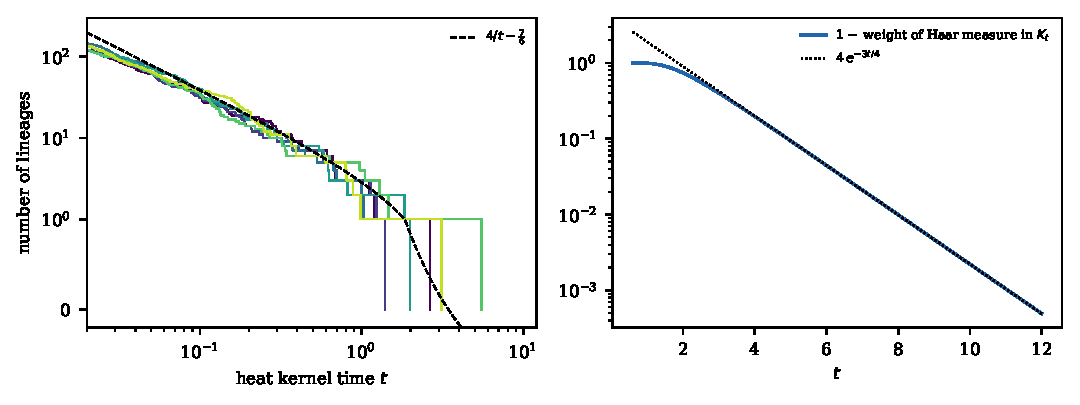
\includegraphics[width=\textwidth]{figures/kingman_fig.pdf}
\caption[Kingman's coalescent in the heat kernel]{Left: six paths of the death process with rates $\frac12m(m+2)$ started from $400$ lineages, against the heat kernel time $t=2\tau$, with the mean $4/t-\frac76$ of the entrance law. Right: one minus the weight of Haar measure in $K_t$, the probability that a lineage survives, with its asymptote $4e^{-3t/4}$; the rate is the gap.}
\label{fig:kingman}
\end{figure}

\section{Three consequences}

\paragraph{\normalfont\scshape A second proof of the likelihood ratio property.} Transition functions of birth and death processes are totally positive, by the theorem of Karlin and McGregor on coincidence probabilities~\cite{KM59}. Start $A$ from $N$. For $s>0$ the law $\delta_NP_s$ is below $\delta_N$ in the likelihood ratio order, as every law on $\{0,\dots,N\}$ is; applying the totally positive kernel $P_t$ preserves the order, so $\delta_NP_{t+s}$ is below $\delta_NP_t$. Let $N\to\infty$: the count of $K_{t+s}$ is below the count of $K_t$. Since $(1+x)^j$ is totally positive in $(j,x)$, the mixtures inherit the order, and $K_t/K_{t+s}$ is increasing in $\cos\theta$. This is Corollary~\ref{cor:mlrall}, with no product formula and no Laguerre: the likelihood ratio property of the heat kernel on SU(2) is the total positivity of Kingman's death process.

\paragraph{\normalfont\scshape The spectral gap is the death of the last lineage.} The time for $A$ to fall from infinity to $m$ is a sum of independent exponential variables with rates $\frac12k(k+2)$, $k>m$: a generalized gamma convolution whose Thorin measure sits on the Casimir values. In particular the weight of Haar measure in the heat kernel is a distribution function,
\[
P_\infty\big(A(t/2)=0\big)=P\Big(\sum_{k\ge1}\frac{2E_k}{k(k+2)}\le\frac t2\Big),
\]
with $E_k$ independent standard exponentials, and the slowest rate, $k=1$, is $\frac32$ in the time $\tau$, which is $\frac34$ in $t$: the spectral gap of the heat semigroup on SU(2), not the mass gap. The heat kernel has become Haar measure exactly when the last lineage has died. This is the cleanest instance in the book of its opening theme: a spectral gap is the lowest atom of a Thorin measure, and here the Thorin measure is that of an extinction time.

\paragraph{\normalfont\scshape The projected ladder is a computable filter.} In counts, the prediction step of the projected ladder is the death process run for a time, and the update step, bond moving, is the addition of independent counts. This is the structure of the exact filter for a Wright Fisher signal: observations add to the count, time removes from it, and the filter never leaves the mixtures of Beta laws. The difference is that the ladder observes itself. The filtering reading of Section~\ref{ch:spdefilter} is thus exact for the prediction and update steps in counts; the projection onto heat kernels is not part of that exactness.

\section{What Kingman's process does not explain}

Decimation in the exact ladder is the convolution of a law with itself, not with a heat kernel, and its kernel $Q(\cdot\mid a,b)$ of Theorem~\ref{thm:coalescence} is not a transition function of $A$. The kernel $Q$ has a genealogical reading: $Q(\cdot\mid a,b)$ is the hypergeometric law of the number of elements common to two random samples of sizes $a$ and $b$ from a population of $a+b+2$ (Theorem~\ref{thm:hypergeometric}).

Nor does duality make the ladder a contraction on all of $\mathcal M$, which it is not. Table~\ref{tab:notmonotone} records one exact rung, $k=4$ and $\ell^2=4$, from several starting laws.

\begin{table}[t]
\centering\small
\begin{tabular}{lccc}
\toprule
starting law & count & change & change of $u_2$ \\ \midrule
heat kernel, $\beta=4$ & 6.87 & $-0.507$ & $-0.017$ \\
$f_5$, a point mass at $5$ & 5.00 & $-0.754$ & \\
Wilson, $\kappa=1$ & 1.24 & $-0.405$ & $-0.053$ \\
Wilson, $\kappa=4$ & 6.63 & $+0.034$ & $+0.021$ \\
Wilson, $\kappa=16$ & 30.5 & $+0.110$ & $+0.002$ \\
half Haar, half $f_{20}$ & 10.0 & $+8.37$ & \\
geometric count, ratio $0.9$ & 8.99 & $+6.50$ & \\
\bottomrule
\end{tabular}
\caption[One exact rung from several starting laws]{The mean count, its change, and the change of the fundamental coefficient over one exact rung of the ladder, from several starting laws in $\mathcal M$. From heat kernels the mean count and the fundamental coefficient fall. From Wilson laws at $\kappa=4$ and $16$ the fundamental coefficient rises at the first rung, and from bimodal laws the count rises sharply. The geometric count is truncated at $100$.}
\label{tab:notmonotone}
\end{table}

Two lessons. A law with two components, one near Haar measure and one concentrated, becomes more ordered under a rung, because raising a density to a power favours its peak; so no functional is monotone on all of $\mathcal M$, and any theorem must be about a class of laws. And the Wilson law at $\kappa\ge2$ gains order at its first rung: bond moving of a Wilson law is exact, $\kappa\mapsto k\kappa$, with none of the curvature loss of Theorem~\ref{thm:scaledmlr}, and the loss appears only once the law has taken the shape of a heat kernel. The inequality $R(\beta)<\beta$ is a statement about the ladder in heat kernel coordinates, as it was stated, and not about one rung from an arbitrary start. We tested two candidate classes on three thousand random laws: when $\nu_0$ is log concave the fundamental coefficient can still rise, by up to $0.03$, and the same is true for sums of independent Bernoulli counts such as a binomial with mean $2$. The orbit of a heat kernel is monotone at every rung we computed. The drift law of Section~\ref{sec:hypergeometric} explains the table to leading order, apart from the Wilson $\kappa=1$ row (count $1.24$, too small for an asymptotic formula) and the geometric row (predicted $+8.56$ against $+6.50$): the change of the mean count is $-\frac{13}{16}+\frac{15}{16}r$ with $r$ the ratio of variance to mean of the count, which is $0$ for a point mass, $\frac13$ for a heat kernel and $1$ for a Wilson law, and $r$ relaxes to $\frac13$ in one or two rungs.

\section{Kingman's other tools}

\paragraph{\normalfont\scshape Random walks with spherical symmetry.} Kingman's paper of 1963~\cite{Ki63} studied the addition of independent random vectors through their lengths alone, and found that the lengths compose by a convolution of their own, indexed by the dimension, with Bessel functions as characters. Convolution of class functions on SU(2) is the compact member of that family: the radial parts of products of independent group elements compose by the Gegenbauer convolution on $[-1,1]$, with the $\chi_n/n$ as characters. Theorem~\ref{thm:coalescence} is a positivity theorem for that convolution on the cone spanned by the powers of $1+x$. Kingman's flat case is the limit of large counts, where $ab/(a+b+2)$ becomes the harmonic rule for precisions.

\paragraph{\normalfont\scshape The subadditive ergodic theorem.} Kingman's theorem~\cite{Ki73} gives the existence of the limit of $\frac1n\log\|X_n\cdots X_1\|$ for stationary products, and with it Lyapunov exponents. Two uses here. The existence of the string tension on the hierarchical lattice in Chapter~\ref{ch:progress} is a deterministic argument of telescoping type, a relative of subadditivity. And the stochastic ladder suggested, and not pursued, in Section~\ref{ch:spdefilter}, a ladder with a common noise at each rung, would have a string tension that is a Lyapunov exponent in Kingman's sense, which exists if the hypotheses of his theorem hold; its positivity is the open question.

\paragraph{\normalfont\scshape Exchangeable partitions.} Kingman's representation of exchangeable partitions through paintbox processes (his paper of 1978) is de Finetti's theorem for partitions, and the Ewens sampling formula~\cite{Ew72} is its best known case. It joins the exchangeability of Chapter~\ref{ch:hitting} to the structure of the ladder.

\section{The genetics volume}

Our \emph{On Statistical Methods for Genetics: Fisher, Ewens and the Bayesian Programme}~\cite{Po26g} treats population genetics as statistical inference. Four of its themes recur here.

\begin{center}
\small
\begin{tabular}{p{0.44\textwidth}p{0.48\textwidth}}
\toprule
genetics volume & this book \\ \midrule
the number of alleles in a sample is a sum of independent Bernoulli variables, and is sufficient for the mutation rate under the Ewens formula & the count $M_0$ of the heat kernel (Proposition~\ref{prop:latentcount}, before reweighting) is a sum of independent Bernoulli variables with parameters $1/\gamma_m$; the action is sufficient for the coupling \\
the Ewens formula from de Finetti's theorem & plaquettes exchangeable under a prior on the coupling; mixtures and their large deviations \\
the number of segregating sites is not sufficient; pooled encoders see only the site frequency spectrum & pooled characters; an attention head finds the sufficient coordinate among eight \\
learned quantile maps for the coalescent attain the Bayes risk & GBC generators for the coupling and for the gap \\
\bottomrule
\end{tabular}
\end{center}

The first row is more than a parallel. In the Ewens formula with parameter $\theta_{\mathrm m}$ the number of alleles among $n$ genes is $\sum_i\xi_i$ with $\xi_i$ Bernoulli of parameter $\theta_{\mathrm m}/(\theta_{\mathrm m}+i-1)$. In the heat kernel the count is $\sum_m\xi_m$ with parameter $1/\gamma_m(t)$. Both are P\'olya frequency laws and the number of alleles is sufficient for $\theta_{\mathrm m}$, as the action is for the coupling. The roots $\gamma_m(t)$ of Theorem~\ref{thm:product} are in this sense the allele probabilities of the heat kernel. The parallel is of the sums, not of the coalescents: the Ewens count is the number of lineages lost to mutation going back in time, while the sum $M_0$ is not the number of lineages that survive to time $t/2$. That number is the latent count $A(t/2)$ of Theorem~\ref{thm:kingman}, whose law is that of $M_0$ reweighted by $C_{m+1}2^{-m}$ (Lemma~\ref{lem:Lcount} and Proposition~\ref{prop:latentcount}).

\section{Are these ideas useful?}

Yes, and more directly than any other neighbour of the ladder. Kingman's coalescent is not an analogy for the ladder on counts; it is the linear half of it. The duality gives a three line proof that heat kernels lie in $\mathcal M$, a second proof of the likelihood ratio property from total positivity of a death process, an identification of the spectral gap of the heat semigroup with the extinction of the last lineage, and the exact filter structure of the projected ladder. What it does not give is the nonlinear half, the self convolution of the exact ladder, and it does not reach $\mathbb Z^4$.

The question it suggests is the right one to end on. Population genetics has a second classical object beside the coalescent: the ancestral graph with selection and recombination, in which lineages branch as well as merge. Bond moving is a branching, by the factor $k$; decimation is a merging. The exact ladder is a branching and coalescing system of lineages, of the kind studied for the ancestral selection graph of Krone and Neuhauser~\cite{KN97}, and its extinction is confinement. Whether the methods that give extinction criteria for such graphs apply here is, as far as we know, an open and well posed question.

\section*{Exercises}
\begin{enumerate}
\item (Section~\ref{sec:hypergeometric}) Verify Lemma~\ref{lem:fjchar} for $j=2$ by expanding $(1+x)^2$ in $\chi_1,\chi_2,\chi_3$.
\item (Section~\ref{sec:hypergeometric}) Compute $Q(\cdot\mid2,3)$ from the Newton formula in the proof and compare with $\big(\frac27,\frac47,\frac17\big)$.
\item Show that $w_N$ is not completely monotone beyond $(N+1)^2$, and explain why the proof needs $\bar a\le\bar b$.
\item Prove that the mean count of the Wilson law is $\kappa$ before reweighting and find it after reweighting, using Corollary~\ref{cor:meancount}.
\item (Section~\ref{sec:wf}) Verify Proposition~\ref{prop:wf} and find the Wright Fisher diffusion that corresponds to the class functions of SU(2) acting on $S^2$ in place of $S^3$.
\item (Section~\ref{sec:duality}) Show from Theorem~\ref{thm:kingman} that the mean count of the heat kernel satisfies $m'(\tau)=-\frac12\E[A(A+2)]$ and deduce $m\approx2/\tau$ for small $\tau$.
\item (Section~\ref{sec:duality}) Compute $P_\infty(A(\tau)=0)$ to three figures at $t=1$ and $t=2$ from the sum of exponentials.
\item For which starting counts $a$ is the law of $A(\tau)$ under $P_a$ log concave for all $\tau$?
\item Find a two point law in $\mathcal M$ whose fundamental coefficient rises under one rung, and explain it by the peak of the bond moved density.
\end{enumerate}

\chapter{Real Zeros}\label{ch:zeros}\index{Lee Yang property}\index{Malo's theorem}\index{real zeros}\index{P\'olya frequency sequence}

Chapter~\ref{ch:counts} left a question: on what class of laws does the exact ladder act well? Its Section~\ref{ch:kingman} showed that log concavity of the count is not the answer to the question of monotonicity. This chapter proposes an answer to the question of invariance, a Lee Yang property \cite{LY52} for the ladder. The heat kernel is a product $\prod_m(1+x/\gamma_m)$ with every $\gamma_m\ge1$: as a function of $x=\cos\theta$ all of its zeros are real and lie to the left of $-1$. We prove that heat flow on the group preserves this property, that the coalescence of Theorem~\ref{thm:coalescence} has it, and we give evidence that the whole exact ladder does.

\section{Two classes}\label{sec:twoclasses}

\begin{definition}
Let $\mathcal L$ be the set of class functions on SU(2) of the form $\rho(x)=c\prod_m(1+x/\gamma_m)$ with $c>0$, $\gamma_m\ge1$ and $\sum_m1/\gamma_m<\infty$, together with their locally uniform limits. Let $\mathcal L'$ be the set of derivatives $F'$, in the variable $x$, of functions $F\in\mathcal L$.
\end{definition}

A member of $\mathcal L$ is an entire function of $x$ whose zeros are all real and at most $-1$; in the variable $z=e^{i\theta}$ its zeros are negative real numbers, in pairs $-e^{\pm\eta}$ with $\gamma=\cosh\eta$. Since $1+x/\gamma=(1-\frac1\gamma)+\frac1\gamma(1+x)$, every member of $\mathcal L$ lies in the family $\mathcal M$ of Chapter~\ref{ch:counts}, with a count $M_0$ that is a sum of independent Bernoulli variables of parameters $1/\gamma_m$; by the theorem of Aissen, Schoenberg, Whitney and Edrei~\cite{Ed52} these are exactly the members of $\mathcal M$ whose count $\nu_0$ is a P\'olya frequency sequence with an entire generating function \cite{ASWE}. By Rolle's theorem $\mathcal L'\subset\mathcal L$.

Three examples. The densities $f_a\propto(1+x)^a$ are in $\mathcal L'$, with $F=(1+x)^{a+1}$. The heat kernel is in $\mathcal L'$: the proof of Theorem~\ref{thm:product} gave $K_t=\frac12\partial_x\vartheta$ with $\vartheta\propto\prod_n(C_n+x)$, so the antiderivative of the heat kernel in $\cos\theta$ is the theta function, which is in $\mathcal L$. The Wilson law $e^{\kappa x}=\lim(1+x/\gamma)^{\kappa\gamma}$ is in the closure of both.

\section{Convolution on SU(2) through the circle}\label{sec:circlecv}

\begin{lemma}\label{lem:circle}
Let $f=\sum_na_n\chi_n$ and $g=\sum_nb_n\chi_n$ be class functions and let $G$ be any antiderivative of $g$ in $x$. Write $\tilde f(z)=f\cdot(z-z^{-1})=\sum_{n\ne0}\operatorname{sgn}(n)\,a_{|n|}z^n$ and $G=\sum_n\hat G_nz^n$. Then $\hat G_n=b_{|n|}/(2|n|)$ for $n\ne0$, and
\[
\widetilde{f*g}(z)=2\sum_{n\ne0}\tilde f_n\,\hat G_n\,z^n .
\]
If also $f=F'$, then $f*g$ is a constant multiple of the derivative in $x$ of the convolution of $F$ and $G$ on the circle.
\end{lemma}

\begin{proof}
$\chi_n=T_n'/n$ with $T_n(\cos\theta)=\cos n\theta$, so $G=\sum_n(b_n/n)\,T_n$ up to a constant, which gives $\hat G_n$. Convolution on the group sends $(a_n,b_n)$ to $a_nb_n/n$, and $\operatorname{sgn}(n)a_{|n|}b_{|n|}/|n|=2\tilde f_n\hat G_n$. The constant term of $G$ plays no part because $\tilde f_0=0$.
\end{proof}

So the convolution of class functions on SU(2) is a Hadamard product of Laurent coefficients, of one function multiplied by $z-z^{-1}$ and an antiderivative of the other. For Hadamard products there is a classical theorem.

\begin{theorem}[Malo \cite{Malo}]\label{thm:malo}
If $P(z)=\sum_ka_kz^k$ has only real zeros and $Q(z)=\sum_kb_kz^k$ has only real zeros, all of the same sign, then $\sum_ka_kb_kz^k$ has only real zeros.
\end{theorem}

\section{What is proved}

\begin{theorem}[real zeros under convolution]\label{thm:zeros}
\begin{enumerate}
\item[(i)] If $f\in\mathcal L$ and $g\in\mathcal L'$ are polynomials with $\deg f\le\deg g$, then $f*g\in\mathcal L$.
\item[(ii)] If $f,g\in\mathcal L'$ are polynomials, then $f*g\in\mathcal L'$.
\item[(iii)] If $f\in\mathcal L$ and $t>0$, then $f*K_t\in\mathcal L$: heat flow on SU(2) preserves the class.
\end{enumerate}
\end{theorem}

\begin{proof}
(i) Let $G\in\mathcal L$ be an antiderivative of $g$, of degree $D=\deg g+1$ in $x$. Then $Q(z)=z^DG$ is a polynomial with only negative zeros, and $P(z)=z^D\tilde f$ is a polynomial, because $\deg f+1\le D$, whose zeros are those of $f$, which are negative, together with $\pm1$ and possibly $0$: all real. By Lemma~\ref{lem:circle} the Hadamard product of $P$ and $Q$ is $\frac12z^D\,\widetilde{f*g}$, which by Malo's theorem has only real zeros. So $f*g$ has only real zeros in $z$, that is, zeros in $x$ that are real and outside $(-1,1)$. Since $f*g$ lies in $\mathcal M$ it is positive for $x>-1$; the zeros are therefore at most $-1$.

(ii) Order the two so that $\deg F\le\deg G$. The Hadamard product of $z^DF$ and $z^DG$ has only real zeros by Malo's theorem and positive coefficients, so the convolution of $F$ and $G$ on the circle is in $\mathcal L$, and by the lemma $f*g$ is its derivative up to a constant.

(iii) For a polynomial $f$, approximate $\vartheta$ by its partial products, which are in $\mathcal L$ and of degree as high as we please, apply (i), and pass to the limit by Hurwitz's theorem. A general $f\in\mathcal L$ is a locally uniform limit of polynomials $f_N\in\mathcal L$ (finite products, or their limits), and we show that $f_N*K_t\to f*K_t$ locally uniformly in complex $x$. Write $x=(z+z^{-1})/2$, let $R>1$, and let $E_R$ be the ellipse that is the image of $|z|=R$. If $F$ is entire in $x$, the Laurent coefficients $\hat F_n$ of $F\big((z+z^{-1})/2\big)$ satisfy $|\hat F_n|\le\max_{E_R}|F|\,R^{-|n|}$ by Cauchy's estimate. Comparing the coefficients of $z^n$ in $F(x)(z-z^{-1})=\sum_{n\ge1}a_n(z^n-z^{-n})$ gives $a_n=\hat F_{n-1}-\hat F_{n+1}$ for the character coefficients $F=\sum a_n\chi_n$, so $|a_n|\le2R\max_{E_R}|F|\,R^{-n}$, and therefore $\sup_nR^n|a_n(f_N)-a_n(f)|\le2R\max_{E_R}|f_N-f|\to0$. The coefficients of $f*K_t$ are $a_ne^{-(n^2-1)t/4}$, and $|\chi_n|\le nR^{n-1}$ on $E_R$, so
\[
\max_{E_R}|f_N*K_t-f*K_t|\le\sup_nR^n|a_n(f_N)-a_n(f)|\sum_{n\ge1}n\,e^{-(n^2-1)t/4}\to0 .
\]
Every compact set lies in some $E_R$, so $f*K_t$ is a locally uniform limit of the functions $f_N*K_t$, which are in $\mathcal L$ by the polynomial case. By the definition of $\mathcal L$, which contains its locally uniform limits, $f*K_t\in\mathcal L$.
\end{proof}

\begin{corollary}[the coalescence has real zeros]\label{cor:coalzeros}
For all integers $a,b\ge0$,
\[
f_a*f_b=c\prod_{i=1}^{\min(a,b)}\Big(1+\frac{x}{\gamma_i(a,b)}\Big),\qquad\gamma_i(a,b)\ge1 .
\]
Hence the count $M_0$ of $f_a*f_b$ is a sum of $\min(a,b)$ independent Bernoulli variables, and the sequence $j\mapsto Q(j\mid a,b)\,2^j/C_{j+1}$ is a P\'olya frequency sequence: in particular it is log concave and unimodal.
\end{corollary}

For example $f_3*f_3$ has zeros $-1.394$, $-3.443$ and $-19.16$. The corollary strengthens Theorem~\ref{thm:coalescence}: the weights of the coalescence kernel are not only positive, after division by $C_{j+1}2^{-j}$ they are the coefficients of a polynomial with only real zeros.

Part (iii) is a statement of the kind that de Bruijn proved on the line \cite{dB50} and that runs through our Riemann volumes: the forward heat flow preserves the reality of zeros. Here the flow is Brownian motion on the group, the variable is $\cos\theta$, and the zeros stay real and to the left of $-1$. In the language of Section~\ref{ch:langlands}, every factor stays Ramanujan under heat flow. In the language of Section~\ref{ch:kingman}, the death process of Kingman's coalescent maps sums of independent Bernoulli counts to sums of independent Bernoulli counts.

\section{An exact case: two Wilson laws}\index{Gegenbauer addition theorem}

One convolution can be done in closed form, and it shows the theorem at work on laws that are not polynomials.

\begin{proposition}[Wilson times Wilson]\label{prop:wilsonwilson}
For $\kappa,\lambda>0$,
\[
e^{\kappa x}*e^{\lambda x}=\frac{2I_1(r)}{r},\qquad r^2=\kappa^2+\lambda^2+2\kappa\lambda x .
\]
Its zeros in $x$ are
\[
x_m=-\frac{\kappa^2+\lambda^2+j_{1,m}^2}{2\kappa\lambda}\ \le\ -1-\frac{j_{1,m}^2}{2\kappa\lambda},\qquad m=1,2,\dots,
\]
where $j_{1,m}$ are the positive zeros of the Bessel function $J_1$. So the convolution of two Wilson laws is in $\mathcal L$, with $\gamma_m=(\kappa^2+\lambda^2+j_{1,m}^2)/(2\kappa\lambda)$, and its count is a sum of independent Bernoulli variables with parameters $2\kappa\lambda/(\kappa^2+\lambda^2+j_{1,m}^2)$.
\end{proposition}

\begin{proof}
Identify SU(2) with the unit sphere of the quaternions, so that $\frac12\operatorname{tr}(V^{-1}U)=\langle V,U\rangle$. Then $(e^{\kappa x}*e^{\lambda x})(U)=\int\exp\langle V,\kappa+\lambda U\rangle\,dV$, the integral of a plane wave over $S^3$, which is $2I_1(|A|)/|A|$ with $A=\kappa+\lambda U$ and $|A|^2=\kappa^2+\lambda^2+2\kappa\lambda\,a_0(U)$. The function $I_1(r)/r$ is even and entire in $r$ with zeros at $r=\pm ij_{1,m}$.
\end{proof}

This is Gegenbauer's addition theorem for Bessel functions in the form it takes on the group. In characters, $e^{\kappa x}=\sum_n(2n/\kappa)I_n(\kappa)\chi_n$, so the statement is $2I_1(r)/r=\sum_n(4n/\kappa\lambda)\,I_n(\kappa)I_n(\lambda)\,\chi_n(x)$, which we also checked numerically to forty figures (\texttt{zeros\_checks.py}). Three things follow.

The zeros are real and to the left of $-1$ by inspection, as Conjecture~\ref{conj:Lclosed} predicts, and the edge $-1$ is attained only in the limit $\kappa\lambda\to\infty$.

The first half of the first rung from a Wilson law is explicit. Bond moving sends $\kappa$ to $k\kappa$ exactly, and one convolution then gives the law $2I_1(r)/r$ with $r=2k\kappa\cos(\theta/2)$: a function of $y=\cos^2(\theta/2)$ alone, with largest zero at $-\gamma_1$, $\gamma_1=1+j_{1,1}^2/(2k^2\kappa^2)$ and $j_{1,1}=3.8317$. For $k\kappa=4$ this is $\gamma_1=1.459$. The zeros have come in from infinity, as Section~\ref{ch:kingman} observed in the count, and the Bernoulli parameters $1/\gamma_m$ of the count are explicit.

The count of this law has a name as well. Expanding, $2I_1(r)/r=\sum_m(r/2)^{2m}/(m!\,(m+1)!)$ with $(r/2)^2=\frac12k^2\kappa^2(1+x)$, so $\nu_0(m)\propto(k^2\kappa^2/2)^m/(m!\,(m+1)!)$: where the Wilson law has a Poisson count, its convolution square has a count with weights $c^m/(m!\,(m+1)!)$, the law of the smaller coordinate of a pair of independent Poisson variables conditioned to differ by one. The product formula for $I_1$ then says that this law is a sum of independent Bernoulli variables, a fact about Bessel numbers that we have not seen stated in this way.

\section{The Thorin form: are Wilson laws generalized gamma convolutions?}\index{generalized gamma convolution}\index{Thorin measure}\index{Hartman Watson law}

The class $\mathcal L$ is the class of this book's title in another variable. If $\rho=c\prod_m(1+x/\gamma_m)$ then
\[
\frac{\rho(0)}{\rho(x)}=\prod_m\frac{\gamma_m}{\gamma_m+x}=\E\,e^{-xT_\rho},\qquad T_\rho=\sum_m\frac{E_m}{\gamma_m},
\]
with independent standard exponential $E_m$. So the reciprocal of a member of $\mathcal L$, as a function of $x=\cos\theta$, is the Laplace transform of a generalized gamma convolution whose Thorin measure \cite{Th77,Bo92} $U_\rho=\sum_m\delta_{\gamma_m}$ has integer masses and is supported on $[1,\infty)$, beyond the edge of the group; limits add a drift. In this dictionary:
\begin{center}
\small
\begin{tabular}{p{0.34\textwidth}p{0.58\textwidth}}
\toprule
law of a link & Thorin measure of $T_\rho$ \\ \midrule
Haar measure & zero \\
$f_a\propto(1+x)^a$ & $a\,\delta_1$, a gamma law of shape $a$ \\
heat kernel $K_t$ & $\sum_m\delta_{\gamma_m(t)}$, atoms moving to the right as $t$ grows \\
Wilson law $e^{\kappa x}$ & zero, with drift $\kappa$: the point mass at $\kappa$ \\
Wilson convolved with Wilson & $\sum_m\delta_{\gamma_m}$, $\gamma_m=(\kappa^2+\lambda^2+j_{1,m}^2)/(2\kappa\lambda)$ \\
bond moving, power $k$ & $U\mapsto kU$, the sum of $k$ independent copies of $T$ \\
heat flow & a map of integer Thorin measures on $[1,\infty)$ to themselves (Theorem~\ref{thm:zeros}) \\
\bottomrule
\end{tabular}
\end{center}
The offset of the Thorin measure, the quantity the first chapters of this book were written about, is $\gamma_1$, the negative of the largest zero, and Conjecture~\ref{conj:Lclosed} below says that convolution on the group acts on integer Thorin measures supported on $[1,\infty)$.

So are Wilson laws related to generalized gamma convolutions? In four ways, of which the first is degenerate and the last is a negative.

\emph{As the boundary case.} The reciprocal of the Wilson law is $e^{-\kappa x}$, the Laplace transform of a point mass: a generalized gamma convolution with no Thorin measure, only drift. The Wilson family is the edge of $\mathcal L$ at which all the atoms have gone to infinity. This is why bond moving costs it nothing and why it has no curvature loss.

\emph{After one convolution.} By Proposition~\ref{prop:wilsonwilson} the reciprocal of $e^{\kappa x}*e^{\lambda x}$ is $r/(2I_1(r))$ with $r^2=\kappa^2+\lambda^2+2\kappa\lambda x$. Chapter~\ref{ch:kacyang} identifies $\sqrt{2s}/(2I_1(\sqrt{2s}))$ as the Laplace transform of the hitting time $\tau$ of the unit sphere $S^3$ by Brownian motion in $\mathbb R^4$, a generalized gamma convolution with Thorin atoms at $\frac12j_{1,m}^2$. Hence
\[
\frac{1}{(e^{\kappa x}*e^{\lambda x})(x)}=\E\Big[e^{-(\kappa^2+\lambda^2)\tau/2}\,e^{-\kappa\lambda\tau\,x}\Big],
\]
the Laplace transform in $x$ of $\kappa\lambda\tau$ under an exponential tilt, and tilting a generalized gamma convolution shifts its Thorin atoms and keeps it in the class. The one plaquette partition function of that chapter is the case $x=1$, $\kappa=\lambda$.

\emph{As a mixture of heat kernels.} The character coefficients of the Wilson law are $u_n=I_n(\kappa)/I_1(\kappa)$. Hartman and Watson \cite{HW74} showed that $I_{\sqrt{2s}}(\kappa)/I_0(\kappa)$ is the Laplace transform of a probability law $\Xi_\kappa$ on the half line, which now carries their names and which Yor \cite{Yor80} found in the windings of planar Brownian motion. Therefore
\[
\frac{I_n(\kappa)}{I_1(\kappa)}=\int e^{-(n^2-1)\xi/2}\,\tilde\Xi_\kappa(d\xi),\qquad\frac{e^{\kappa x}}{Z(\kappa)}=\int K_{2\xi}\,\tilde\Xi_\kappa(d\xi),
\]
with $\tilde\Xi_\kappa$ the Hartman Watson law tilted by $e^{-\xi/2}$: the Wilson law is a mixture of heat kernels over a random time. The Hartman Watson law is infinitely divisible, and it is known to lie in the Bondesson class \cite{Ke78,Bo92}, whose members have a complete Bernstein function as the negative logarithm of the Laplace transform; that class contains the generalized gamma convolutions. This mixture is the original theorem of Hartman and Watson, whose title speaks of normal distribution functions on spheres: the von Mises Fisher law on a sphere, which on $S^3$ is the Wilson law, is a mixture of the Brownian, or normal, laws on the sphere, which are the heat kernels. Hartman's paper of 1976 \cite{Har76} on completely monotone families of solutions of linear differential equations then gave the general mechanism, for Bessel functions and beyond, by which such ratios are Laplace transforms of infinitely divisible laws; read in the language of our Riemann volumes it is a scale mixture of normals result of the extended generalized gamma convolution kind, with the heat kernel in the part of the normal law and the Hartman Watson time in the part of the mixing variance. Whether the Hartman Watson law is itself a generalized gamma convolution in the strict sense is settled in the next section. It is one, with an explicit Thorin measure, and the Wilson action is a Thorin mixture of heat kernel actions.

\emph{As a law on the group, no.} The law of $1-\cos\theta$ under the Wilson measure lives on $[0,2]$, and a nondegenerate generalized gamma convolution has unbounded support. Only in the weak coupling scaling does it become one: $\kappa(1-\cos\theta)$ tends to a gamma law of shape $\frac32$.

\begin{figure}[t]
\centering
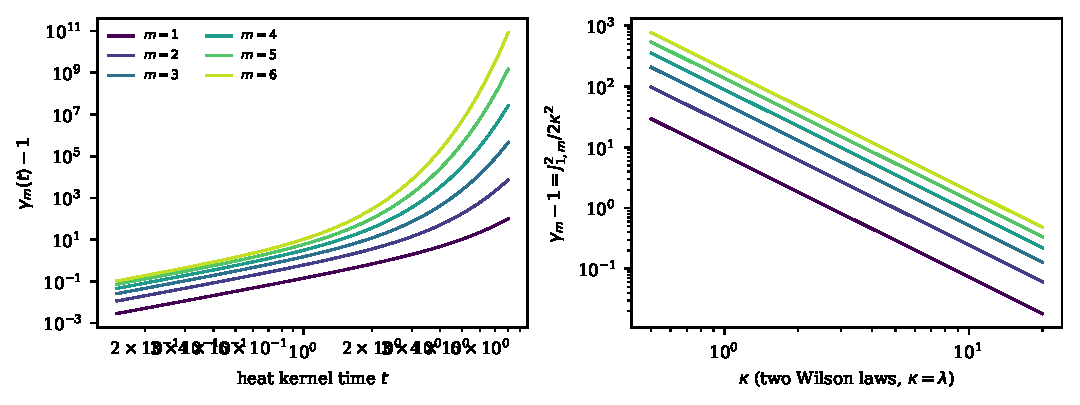
\includegraphics[width=\textwidth]{figures/zeros_fig.pdf}
\caption[Zeros of the heat kernel and of two Wilson laws]{The Thorin atoms $\gamma_m$, shown as $\gamma_m-1$, the distance of the zeros of the link density from the edge $\cos\theta=-1$. Left: the first six for the heat kernel, increasing in $t$. Right: for the convolution of two Wilson laws of equal coupling, where $\gamma_m-1=j_{1,m}^2/2\kappa^2$.}
\label{fig:zeros}
\end{figure}

\section{The Hartman Watson law is a generalized gamma convolution}\label{sec:hwggc}\index{Hartman Watson law!Thorin measure}\index{Neumann's product formula}\index{P\'olya, G.}

Fix $r>0$ and let $\Xi_r$ be the Hartman Watson law, with $\int e^{-s\xi}\,\Xi_r(d\xi)=I_{\sqrt{2s}}(r)/I_0(r)$. Write
\[
\phi_r(y)=\arg I_{iy}(r),\qquad y\ge0,\quad\phi_r(0)=0,
\]
for the continuous phase of the Bessel function of imaginary order.

\begin{theorem}[Thorin form of the Hartman Watson law]\label{thm:hwggc}
For every $r>0$ and $y\ge0$,
\[
\phi_r'(y)=-\frac{2}{\pi\,|I_{iy}(r)|^2}\int_0^{\pi/2}K_0(2r\cos a)\,\cosh(2ya)\,da<0,
\]
and $\Xi_r$ is a generalized gamma convolution without drift:
\[
\frac{I_{\sqrt{2s}}(r)}{I_0(r)}=\exp\Big(-\int_0^\infty\log\Big(1+\frac sq\Big)U_r(dq)\Big),\qquad U_r\big([0,\tfrac12y^2]\big)=-\frac{\phi_r(y)}{\pi}.
\]
\end{theorem}

\begin{proof}
Neumann's product formula \cite[\S5.43]{Wat44} reads, for $\operatorname{Re}(\mu+\nu)>-1$,
\[
I_\mu(r)\,I_\nu(r)=\frac2\pi\int_0^{\pi/2}I_{\mu+\nu}(2r\cos a)\,\cos\big((\mu-\nu)a\big)\,da .
\]
Put $\mu=\sigma+iy$ and $\nu=\sigma-iy$. Since $I_{\bar\nu}(r)=\overline{I_\nu(r)}$ the left side is $|I_{\sigma+iy}(r)|^2$, and the right side is positive for $\sigma>-\frac12$; so $I_\nu(r)$ has no zeros in $\operatorname{Re}\nu>-\frac12$, and $\log I_\nu(r)$ is analytic there. Differentiate in $\sigma$ at $\sigma=0$, using $\partial_\sigma I_\sigma(z)|_{\sigma=0}=-K_0(z)$:
\[
2\operatorname{Re}\Big(\overline{I_{iy}(r)}\;\partial_\nu I_\nu(r)\big|_{\nu=iy}\Big)=-\frac4\pi\int_0^{\pi/2}K_0(2r\cos a)\cosh(2ya)\,da .
\]
Dividing by $2|I_{iy}|^2$ gives $\operatorname{Re}\partial_\nu\log I_\nu(r)$ at $\nu=iy$, and that is $\phi_r'(y)$, because $\partial_\nu=-i\partial_y$ on the imaginary axis. This is the first statement. For the second put $G(\nu)=-\partial_\nu\log I_\nu(r)$. It is analytic in the closed right half plane, real on the real axis, of logarithmic growth, and its real part on the imaginary axis is $-\phi_r'(|y|)\ge0$. The Poisson formula for the half plane, with the two halves of the axis taken together, gives
\[
G(\nu)=\frac{2\nu}{\pi}\int_0^\infty\frac{-\phi_r'(y)}{\nu^2+y^2}\,dy ,
\]
with no linear term because $G(\nu)/\nu\to0$. With $\nu=\sqrt{2s}$ and $q=\frac12y^2$ this is
\[
-\frac{d}{ds}\log I_{\sqrt{2s}}(r)=\frac{G(\nu)}{\nu}=\int_0^\infty\frac{U_r(dq)}{s+q},\qquad U_r(dq)=-\frac{\phi_r'(y)}{\pi}\,dy,
\]
a Stieltjes transform of a positive measure, and integrating from $0$ to $s$ gives the representation. The integrability conditions on a Thorin measure hold because $-\phi_r'(y)$ tends to $K_0(r)/I_0(r)$ at $0$ and grows like $\log(2y/r)$ at infinity.
\end{proof}

We have not found this statement in the literature, where the law is known to be infinitely divisible and of the Bondesson class; it may be known to specialists, and the proof is two lines once Neumann's formula is differentiated in the right variable. Numerically (\texttt{hw\_thorin.py}) the formula for $\phi_r'$ agrees with a difference quotient of the phase to six figures, and the representation reproduces $\log\big(I_{\sqrt{2s}}(r)/I_0(r)\big)$ to three or four, the limit of our quadrature of the tail. The same differentiation in $y$ instead of $\sigma$ shows that $|I_{iy}(r)|$ increases in $y$. Figure~\ref{fig:hwthorin} shows the Thorin density.

\begin{figure}[t]
\centering
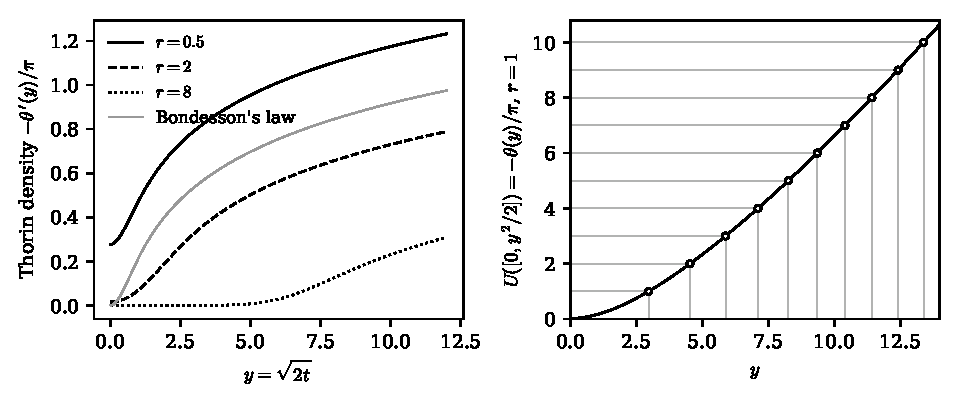
\includegraphics[width=\textwidth]{figures/hw_thorin.pdf}
\caption[The Thorin measure of the Hartman Watson law]{Left: the Thorin density of the Hartman Watson law in the variable $y=\sqrt{2q}$, for three values of $r$, with that of Bondesson's law $e^{-\gamma_{\mathrm E}\nu}/\Gamma(1+\nu)$. Right: the Thorin distribution function at $r=1$; it takes the value $n$ exactly at the $n$th zero of P\'olya's function $K_{iy}(1)$, marked by circles.}
\label{fig:hwthorin}
\end{figure}

\begin{corollary}[the Wilson action is a Thorin mixture of heat kernels]\label{cor:wilsonthorin}
The mixing law $\tilde\Xi_\kappa$ in $e^{\kappa x}/Z(\kappa)=\int K_{2\xi}\,\tilde\Xi_\kappa(d\xi)$ is a generalized gamma convolution, with Thorin measure that of $\Xi_\kappa$ moved to the right by $\frac12$:
\[
\frac{I_n(\kappa)}{I_1(\kappa)}=\exp\Big(\frac1\pi\int_0^\infty\log\Big(1+\frac{n^2-1}{1+y^2}\Big)\phi_\kappa'(y)\,dy\Big).
\]
Its Thorin measure is supported on $[\frac12,\infty)$, so $\tilde\Xi_\kappa$ has exponential moments of every order below $\frac12$.
\end{corollary}

\begin{proof}
An exponential tilt $e^{-c\xi}$ of a generalized gamma convolution replaces $\log(1+s/q)$ by $\log\big(1+s/(q+c)\big)$. Here $c=\frac12$, $s=\frac12(n^2-1)$ and $q=\frac12y^2$.
\end{proof}

At $\kappa=2$ the right side, by the quadrature of \texttt{hw\_thorin.py}, gives $\log(I_2/I_1)=-0.8367$ and $\log(I_4/I_1)=-3.4457$ against the exact $-0.8367$ and $-3.4454$. The corollary answers the question the last section ended on. The gap $\frac34$ of a heat kernel at unit time, mixed over a law whose Thorin measure begins at $\frac12$, is how the Wilson law carries its own first character.

\paragraph{\normalfont\scshape The von Mises law and the extended class.} The theorem of Hartman and Watson was stated for spheres in every dimension, and on the circle it says that the von Mises law is a mixture of wrapped normal laws over $\Xi_\kappa$. A normal law with variance drawn from a generalized gamma convolution is an extended generalized gamma convolution in Thorin's and Bondesson's sense, so by Theorem~\ref{thm:hwggc} the von Mises law is such a law on the line, wrapped round the circle. On SU(2) the heat kernel takes the place of the normal law and the Wilson law that of the von Mises law. This is the sense in which Hartman's result of 1976 is a scale mixture of normals result of the extended kind: his complete monotonicity gives the mixture, and the theorem above places the mixing law in Thorin's class.

\paragraph{\normalfont\scshape Four links with the Riemann volumes.} The theorem sits closer to our \emph{Computing the Riemann Hypothesis} \cite{PS26a,PS26b,PS26c} than any other result of this book.

First, the substitution. The Polson $2\sin^2$ lemma, Lemma~\ref{lem:2sin2B}, passes from a transform in $w$ to a Thorin measure in $u=\frac12w^2$, and its kernel is $1-\cos(xy)=2\sin^2(\frac12xy)$ with $y=\sqrt{2z}$ in the notation of the lemma, where $x$ is the variable called $\omega$ below. Here $w$ is the order $\nu$ of the Bessel function and $u$ is $s$. If $\nu\mapsto I_\nu(r)$ has only real zeros $-a_k$, then
\[
-\log\frac{I_\nu(r)}{I_0(r)}=\frac{K_0(r)}{I_0(r)}\,\nu+\int_0^\infty\big(e^{-\nu\omega}+\nu\omega-1\big)\sum_ke^{-a_k\omega}\,\frac{d\omega}{\omega},
\]
a compensated transform of a positive measure, and the lemma gives the Thorin density at once as
\[
-\phi_r'(y)=\frac{K_0(r)}{I_0(r)}+\sum_k\frac{y^2}{a_k(a_k^2+y^2)} .
\]
Theorem~\ref{thm:hwggc} proves the positivity of the left side without knowing where the zeros are; the argument above shows only that none has real part above $-\frac12$. So it is an instance in which the conclusion of the lemma holds and the reality of the zeros behind it is, as far as we know, open, the reverse of the situation for the Riemann xi function, where one wants the zeros and has the lemma.

Second, the phase. In the Riemann volumes the Thorin measure of the reciprocal xi function at the centre is the counting measure of the zeros at $\frac12\gamma^2$, and its smooth part is the derivative of the phase of the gamma factor. Here the Thorin measure is exactly the derivative of a phase, $-\phi_r'(y)/\pi$, and for large $y$ that phase is $-\arg\Gamma(1+iy)+y\log\frac12r$: the same function, with density $\frac1\pi\log(2y/r)$ in place of $\frac1{2\pi}\log(T/2\pi)$.

Third, P\'olya. The imaginary part of $I_{iy}(r)$ is $-\sinh(\pi y)K_{iy}(r)/\pi$, and $K_{iy}(r)$ is the function whose zeros in $y$ P\'olya proved real in 1926, in his study of approximations to the xi function \cite{Po26}. Since the phase is strictly decreasing it passes through the multiples of $\pi$ once each, and exactly at those zeros. Hence
\[
\#\{0<y\le Y:\ K_{iy}(r)=0\}=\big\lfloor U_r\big([0,\tfrac12Y^2]\big)\big\rfloor :
\]
the Thorin distribution function of the Hartman Watson law counts P\'olya's zeros. At $r=1$ (\texttt{hw\_thorin.py}) the first ten zeros are at $y=2.9625$, $4.5345$, \dots, $13.3859$, and $-\phi_1/\pi$ there is $1.0000$, $2.0000$, \dots, $10.0000$. It is a Riemann and von Mangoldt formula for P\'olya's function with no error term, and it is the Hermite and Biehler picture of the volumes: $I_{iy}$ is the structure function and $K_{iy}$ its odd part.

Fourth, Bondesson's letter. As $r\to0$, $I_\nu(r)/I_0(r)$ tends to $(r/2)^\nu/\Gamma(1+\nu)$, which is $e^{-\gamma_{\mathrm E}\nu}/\Gamma(1+\nu)$ times $e^{-(\log(2/r)-\gamma_{\mathrm E})\nu}$. The first factor, in $\nu=\sqrt{2s}$, is up to scale the law of Bondesson's letter of 2016 printed in the first Riemann volume \cite{PS26a}, with Thorin density $\frac1\pi\big(\gamma_{\mathrm E}+\operatorname{Re}\psi(1+iy)\big)$; the second is the hitting time of a level by Brownian motion. So the Hartman Watson laws are a one parameter family that ends, at small $r$, in Bondesson's law convolved with a stable law of index one half, and at every $r$ the density at $y=0$ is $K_0(r)/\pi I_0(r)$, the stable part.

\paragraph{\normalfont\scshape What it gives the mass gap.} Not the gap. It relates the two actions of this book, which Section~\ref{ch:kingman} found to behave differently at the first rung, by a mixture inside Thorin's class: any statement proved for heat kernels that is linear in the law, or stable under such mixtures, passes to Wilson's action. Which of the statements of this book are of that kind is the question to ask next; the contraction of Theorem~\ref{thm:scaledmlr} is not, since bond moving is not linear.

\section{A sharper criterion: Schur and Szeg\H o}\label{sec:szego}\index{Schur Szeg\H o composition}\index{multiplier sequence}\index{de la Vall\'ee Poussin kernel}

Theorem~\ref{thm:zeros} asks that one factor have an antiderivative in $\mathcal L$, and most members of $\mathcal L$ have none: of random polynomials in $\mathcal L$ of degree $3$, $6$ and $12$, about $81$, $28$ and $3$ per cent do (\texttt{szego\_criterion.py}). The hypothesis can be weakened a great deal by using, in place of Malo's theorem, the composition theorem from which it descends.

\begin{theorem}[Schur and Szeg\H o \cite{Sz22}]\label{thm:schurszego}
If $A(z)=\sum_{k=0}^n\binom nka_kz^k$ has only real zeros and $B(z)=\sum_{k=0}^n\binom nkb_kz^k$ has only real zeros, all of the same sign, then $\sum_{k=0}^n\binom nka_kb_kz^k$ has only real zeros.
\end{theorem}

In the language of P\'olya and Schur, $B$ is the Jensen polynomial of the sequence $(b_k)$, and the theorem says that a sequence whose Jensen polynomial of degree $n$ has real zeros of one sign multiplies the coefficients of every real polynomial of degree $n$ with real zeros into another such. Malo's theorem is the case in which $\sum b_kz^k$ itself has real zeros of one sign.

\begin{theorem}[the smoothed criterion]\label{thm:szegocriterion}
Let $f,g\in\mathcal L$ be polynomials of degrees $d$ and $D$. If $f*f_D\in\mathcal L'$, or if $g*f_d\in\mathcal L'$, then $f*g\in\mathcal L$.
\end{theorem}

\begin{proof}
Suppose $f*f_D\in\mathcal L'$, and put $N=D+1$. As in the proof of Theorem~\ref{thm:zeros}, $P(z)=z^N\tilde g(z)$ is a polynomial of degree $2N$ with only real zeros, and by Lemma~\ref{lem:circle} the coefficients of $z^N\,\widetilde{f*g}$ are those of $P$ multiplied by $q_m=a_{|m|}/|m|$ at the power $z^{N+m}$, $m\ne0$, where $f=\sum a_n\chi_n$; the coefficient of $z^N$ in $P$ is zero, so $q_0$ is at our disposal. The Jensen polynomial of this sequence is
\[
\sum_{m=-N}^{N}\binom{2N}{N+m}q_m\,z^{N+m}=z^N\Big(c+2\sum_{m\ge1}\binom{2N}{N+m}\frac{a_m}{m}\,T_m(x)\Big),
\]
with $x=\frac12(z+z^{-1})$. Since $(1+x)^N=2^{-N}\sum_m\binom{2N}{N+m}z^m$, the density $f_D\propto(1+x)^{N-1}$ has character coefficients proportional to $m\binom{2N}{N+m}$, so $f*f_D$ is proportional to $\sum_m\binom{2N}{N+m}a_m\chi_m$, and the bracket is an antiderivative in $x$ of a multiple of $f*f_D$, with $c$ free. By hypothesis $c$ can be chosen so that the bracket is in $\mathcal L$; then the Jensen polynomial has only negative zeros and a possible zero at the origin, and Theorem~\ref{thm:schurszego} gives $z^N\,\widetilde{f*g}$ only real zeros. So the zeros of $f*g$ in $x$ are real and outside $(-1,1)$, and since $f*g\in\mathcal M$ they are at most $-1$. The other case is the same with $f$ and $g$ exchanged.
\end{proof}

Three remarks on what has been gained.

\emph{It contains the old theorem.} If $f\in\mathcal L'$ then $f*f_D\in\mathcal L'$ by Theorem~\ref{thm:zeros}(ii), since every $f_D$ is in $\mathcal L'$.

\emph{It is a statement about one function.} The hypothesis does not involve $g$ beyond its degree. And it gives more than was asked: when it holds, convolution with $f$ carries every real polynomial of degree $2D+2$ in $z$ with real zeros to another, not only those that come from $\mathcal L$. The laws $f$ for which this is so, for a given $D$, are closed under convolution with each other, because their multiplier sequences multiply termwise.

\emph{It is a smoothing.} The binomial weights are the Fourier coefficients of $\cos^{2N}(\theta/2)$, the kernel of de la Vall\'ee Poussin, so the bracket is the antiderivative of $f$ smoothed on the circle by that kernel, which is close to a heat kernel at time $4/N$. An antiderivative of a function with real zeros need not have real zeros; the criterion asks only that it have them after a smoothing whose strength is matched to the degree of the other factor. This is de Bruijn's phenomenon again: smoothing moves zeros onto the real axis.

\begin{figure}[t]
\centering
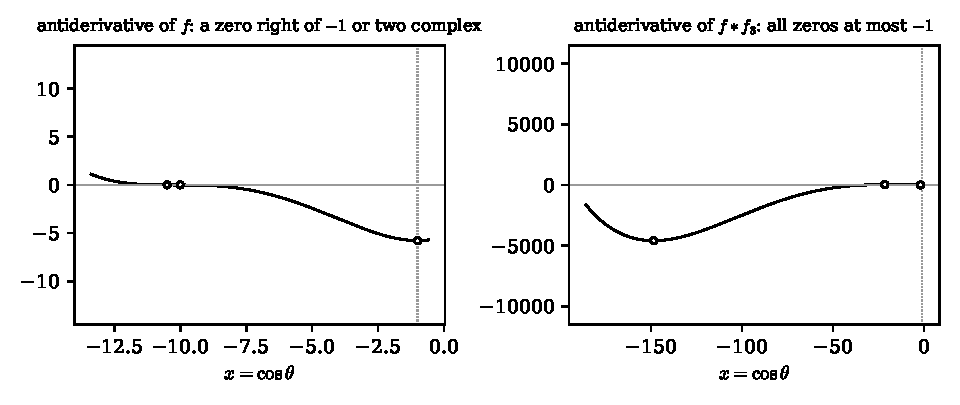
\includegraphics[width=\textwidth]{figures/szego_smoothing.pdf}
\caption[Smoothing makes the antiderivative real rooted]{The law $f=(1+x)(1+x/10)(1+x/10.5)$ is in $\mathcal L$ and not in $\mathcal L'$. Left: its antiderivative, with the constant chosen as well as it can be; the circles are the zeros of $f$, and the fourth zero falls to the right of $-1$. Right: the antiderivative of $f*f_3$, which has four real zeros at most $-1$, so that Theorem~\ref{thm:szegocriterion} applies to $f*g$ for every cubic $g\in\mathcal L$.}
\label{fig:szego}
\end{figure}

Does the hypothesis hold? In every case we have tried, when the degrees are comparable.

\begin{center}
\small
\begin{tabular}{cccc}
\toprule
degree of $f$ & $D$ & $f\in\mathcal L'$ & $f*f_D\in\mathcal L'$ \\ \midrule
$3$ & $3$ & $0.81$ & $1.00$ \\
$6$ & $6$ & $0.28$ & $1.00$ \\
$9$ & $9$ & $0.18$ & $1.00$ \\
$12$ & $12$ & $0.03$ & $1.00$ \\
$4$ & $12$ & $0.49$ & $1.00$ \\
\bottomrule
\end{tabular}
\end{center}

Each row (\texttt{szego\_criterion.py}, seed $3$) is $120$ polynomials in $\mathcal L$ with zeros spread over four decades, split into a cluster near $-1$ and a cluster far away, or of two zeros with high multiplicity, in $120$ digit arithmetic. In the other direction, for $g$ of degree $6$ to $12$ and $d$ from $1$ to $5$, $g*f_d$ was in $\mathcal L'$ in all $480$ trials, $80$ for each of six pairs $(\deg g,d)$. The laws that the old theorem could not reach are covered: for bond moved laws $\rho^k$ with $k=2$ and $4$, with two or more distinct zeros, all of even multiplicity, so that they are never in $\mathcal L'$, the smoothed law $\rho^k*f_d$ was in $\mathcal L'$ in each of six cases, among them $\rho=(1+x/1.2)(1+x/2)(1+x/5)$ and $\rho=(1+x/1.001)(1+x/1000)$. The hypothesis $f*f_D\in\mathcal L'$ does fail when $D$ is much larger than the degree of $f$, as it must, since $f*f_D\to f$: for $f=(1+x)(1+x/10)(1+x/10.5)$ it holds for $D=3$, $6$ and $12$ and fails for $D=24$. That is why the theorem has two cases, and the second, in which the factor of higher degree is smoothed by the lower, is the one that has not failed.

\begin{conjecture}[smoothing]\label{conj:smoothing}
If $g\in\mathcal L$ is a polynomial and $d\le\deg g$, then $g*f_d\in\mathcal L'$: the convolution of $g$ with $(1+\cos\theta)^d$ has an antiderivative in $\cos\theta$ with only real zeros, all at most $-1$.
\end{conjecture}

By Theorem~\ref{thm:szegocriterion}, Conjecture~\ref{conj:smoothing} implies Conjecture~\ref{conj:Lclosed} for polynomials, and for their limits by the estimate in the proof of Theorem~\ref{thm:zeros}(iii), applied to two factors, for which the products $a_nb_n/n$ of character coefficients are $O(R^{-2n})$ for every $R$. It is a statement about a single function and a single explicit kernel in place of a statement about all pairs, and for $d\le2$ its second half is automatic, since every polynomial of degree at most two in $\mathcal L$ is in $\mathcal L'$. We have not proved it. Two attempts that fail are worth a line each. Laguerre's theorem, that an entire function of the Laguerre and P\'olya class without zeros in $[0,n]$ gives a multiplier for polynomials of degree $n$, would do it if the character coefficients $b_m/m$ had such an interpolation in $m$; the natural even interpolation, a combination of the functions $1/\Gamma(J+1-s)\Gamma(J+1+s)$, has complex zeros in $214$ of $300$ random trials (\texttt{zeros\_checks.py}, seed $2$: $g$ of degree $2$ to $6$ with $\gamma-1=10^U$, $U$ uniform on $(-2,3)$, and the constant of integration fixed by $G(-1)=0$). And writing the convolution as a mixture over an auxiliary variable of polynomials each of which has real zeros, which can be done explicitly, proves nothing, since mixtures do not keep real zeros.

\section{The radial flow, and a criterion by signs}\label{sec:radial}\index{radial flow}\index{interlacing}

A third approach to Conjecture~\ref{conj:Lclosed} compares the convolution on SU(2) with the convolution on the circle, for which the conjecture is Malo's theorem. For class functions write
\[
(f\circledast g)(\cos\theta)=\frac1{2\pi}\int_0^{2\pi}f(\cos\psi)\,g(\cos(\theta-\psi))\,d\psi,
\]
and put $\mathcal D_sf(x)=f(sx)$ and $Ef=x\,f'(x)$.
If $f,g\in\mathcal L$ then $\mathcal D_sf,\mathcal D_sg\in\mathcal L$ for $0<s\le1$, their zeros being those of $f$ and $g$ divided by $s$; and $f\circledast g$ has only real zeros, all at most $-1$, because in the variable $z$ it is the Hadamard product of two polynomials with negative zeros.

\begin{theorem}[radial flow]\label{thm:radialflow}
For class functions $f,g$ and $0<s\le1$,
\[
s^2\,(\mathcal D_sf*\mathcal D_sg)=\int_0^s2\varrho\,(\mathcal D_\varrho f\circledast \mathcal D_\varrho g)\,d\varrho,\qquad\frac{d}{ds}\big[s^2(\mathcal D_sf*\mathcal D_sg)\big]=2s\,(\mathcal D_sf\circledast \mathcal D_sg),
\]
and
\[
f\circledast g=f*g+\tfrac12\,(Ef)*g+\tfrac12\,f*(Eg).
\]
If $f=\prod_{i\le d}(1+x/\gamma_i)$ and $g=\prod_{k\le D}(1+x/\delta_k)$, and $f_{\setminus i}$, $g_{\setminus k}$ denote the products with one factor removed, then
\[
\Big(1+\frac{d+D}{2}\Big)\,f*g=f\circledast g+\frac12\sum_{i=1}^df_{\setminus i}*g+\frac12\sum_{k=1}^Df*g_{\setminus k}.
\]
\end{theorem}

\begin{proof}
By Lemma~\ref{lem:ellipse} and its proof, $(f*g)(\cos\theta)=\frac1\pi\int_{|p|<1}f(p\cdot u)\,g(p\cdot e_\theta)\,d^2p$ over the unit disc, with $u$ and $e_\theta$ unit vectors at angle $\theta$. Replacing $f,g$ by $\mathcal D_sf,\mathcal D_sg$ and $p$ by $p/s$ gives $s^2(\mathcal D_sf*\mathcal D_sg)=\frac1\pi\int_{|p|<s}f(p\cdot u)g(p\cdot e_\theta)\,d^2p$, and in polar coordinates the integral over the circle of radius $\varrho$ is $2\pi\,(\mathcal D_\varrho f\circledast \mathcal D_\varrho g)$. That is the first identity. For the second apply the divergence theorem on the unit disc to the field $p\,f(p\cdot u)g(p\cdot e_\theta)$, whose divergence is $2fg+(Ef)g+f(Eg)$ and whose flux through the boundary is $2\pi(f\circledast g)$. For the third, $Ef=\sum_ixf/(x+\gamma_i)=d\,f-\sum_if_{\setminus i}$.
\end{proof}

So the convolution on SU(2) is the running average, over the radius, of convolutions on the circle of dilated laws, each of which has real zeros. A mixture of polynomials with real zeros need not have real zeros; but this mixture is a flow, and a flow keeps real zeros as long as the polynomial and its derivative along the flow interlace.

\begin{proposition}[the flat limit]\label{prop:flatlimit}
Let $f=\sum_kf_kx^k$ and $g=\sum_kg_kx^k$ be polynomials in $\mathcal L$. As $s\to0$ the zeros of $\mathcal D_sf*\mathcal D_sg$ are asymptotic to $y_i/s^2$, where the $y_i$ are the zeros of
\[
Q(y)=\sum_k\frac{f_kg_k}{k+1}\Big(\frac y2\Big)^k,
\]
and $Q$ has only real negative zeros. The zeros of $\mathcal D_sf\circledast \mathcal D_sg$ are asymptotic to those of $P(y)=\sum_kf_kg_k(y/2)^k$ divided by $s^2$, and $P=(yQ)'$, so the zeros of $P$ interlace those of $Q$.
\end{proposition}

\begin{proof}
The coefficient of $x^k$ in $E(u\cdot v)^j(e\cdot v)^{j'}$ over $S^3$ vanishes unless $j,j'\ge k$, and for $j=j'=k$ it is the number $k!$ of perfect matchings between the two groups times the constant $1/2^k(k+1)!$ of the proof of Theorem~\ref{thm:matching}; on the circle the constant is $1/2^kk!$. The lowest order in $s$ of the coefficient of $x^k$ is therefore $s^{2k}f_kg_k/2^k(k+1)$, and $s^{2k}f_kg_k/2^k$ on the circle. By Schur's theorem $\sum_kk!\,f_kg_ky^k$ has only real negative zeros, $f$ and $g$ having negative zeros, and $1/(k+1)!$ is a multiplier sequence of the first kind, by Laguerre's theorem. The last statement is Rolle's.
\end{proof}

\begin{theorem}[closure follows from the absence of a common zero]\label{thm:flowclosure}
Let $f,g\in\mathcal L$ be polynomials, and suppose the polynomial $Q$ of Proposition~\ref{prop:flatlimit} has simple zeros. If for no $s\in(0,1]$ do $\mathcal D_sf*\mathcal D_sg$ and $\mathcal D_sf\circledast \mathcal D_sg$ have a common zero, then $f*g\in\mathcal L$, and the zeros of $f\circledast g$ strictly interlace those of $f*g$, each zero of $f*g$ lying to the left of the corresponding zero of $f\circledast g$. In that case the zeros of $\mathcal D_sf*\mathcal D_sg$ increase strictly with $s$.
\end{theorem}

\begin{proof}
Put $\Phi_s=s^2(\mathcal D_sf*\mathcal D_sg)$ and $\Psi_s=\mathcal D_sf\circledast \mathcal D_sg$, polynomials in $x$ of the same degree with positive leading coefficients, and $\partial_s\Phi_s=2s\Psi_s$. By Proposition~\ref{prop:flatlimit}, for small $s$ the zeros of $\Phi_s$ are real and simple and strictly interlaced by those of $\Psi_s$. Let $s^*$ be the supremum of the $s$ up to which this holds. At $s^*$ the zeros of $\Phi$ are real and weakly interlaced by those of $\Psi$, which are real by Malo's theorem. A double zero of $\Phi_{s^*}$, or a failure of strictness, would put a zero of $\Psi_{s^*}$ on a zero of $\Phi_{s^*}$, which is excluded. So the interlacing is strict at $s^*$, and being an open condition it persists, whence $s^*=1$. With strict interlacing, $\Psi_s$ has at each zero of $\Phi_s$ the sign opposite to that of $\Phi_s'$, so every zero moves to the right.
\end{proof}

A second criterion uses the last identity of Theorem~\ref{thm:radialflow} and nothing else.

\begin{theorem}[a criterion by signs]\label{thm:signcriterion}
Let $f,g\in\mathcal L$ be polynomials of degrees $d$ and $D$, let $n=\min(d,D)$, and let $\psi_1>\psi_2>\dots>\psi_n$ be the zeros of $f\circledast g$, assumed simple. If each of the $d+D$ lower convolutions $f_{\setminus i}*g$ and $f*g_{\setminus k}$ has the sign $(-1)^{j-1}$ at $\psi_j$, for $j=1,\dots,n$, then $f*g$ has $n$ real zeros, one in each interval $(\psi_{j+1},\psi_j)$ and one to the left of $\psi_n$; in particular $f*g\in\mathcal L$.
\end{theorem}

\begin{proof}
At $\psi_j$ the right side of the identity is half the sum of the lower convolutions, so $f*g$ has the sign $(-1)^{j-1}$ there. It has degree $n$ and a positive leading coefficient, so its sign at $-\infty$ is $(-1)^n$, opposite to its sign at $\psi_n$. That gives $n$ changes of sign, and all the zeros are below $\psi_1\le-1$.
\end{proof}

The hypothesis says that each lower convolution, in which one factor has been removed from $f$ or from $g$, is interlaced by the circle convolution of the full pair. It is the natural statement to carry in an induction on $d+D$: the lower convolutions are in $\mathcal L$ by the inductive hypothesis, each is interlaced by its own circle convolution $f_{\setminus i}\circledast g$, and that in turn interlaces $f\circledast g$ because a Hadamard product with a polynomial with negative zeros preserves interlacing. What the induction lacks is the passage from these two interlacings to the third, of $f_{\setminus i}*g$ with $f\circledast g$: both have their $j$th zeros in the same gap of the zeros of $f_{\setminus i}\circledast g$, and the order of the two within the gap is what must be shown.

Both hypotheses hold in every case we have computed (\texttt{radial\_flow.py}), in $80$ digit arithmetic. Along the flow, for $60$ pairs of degrees $2$ to $8$ with zeros spread over five decades or repeated, at $40$ values of $s$ each, the zeros of $\mathcal D_sf*\mathcal D_sg$ were real, strictly interlaced by those of $\mathcal D_sf\circledast \mathcal D_sg$, and increasing in $s$; the smallest gap between a zero of one and the nearest zero of the other, relative to its size, was $0.064$, so a common zero was never approached. And the sign condition held for all $1037$ lower convolutions of $120$ pairs. The identities of Theorem~\ref{thm:radialflow} hold to the precision of the arithmetic, and at $s=\frac1{200}$ the scaled zeros agree with those of $Q$ to five figures.

\begin{conjecture}[interlacing]\label{conj:interlacing}
For polynomials $f,g\in\mathcal L$ the zeros of the circle convolution $f\circledast g$ strictly interlace those of the SU(2) convolution $f*g$, each zero of $f*g$ lying to the left of the corresponding zero of $f\circledast g$.
\end{conjecture}

Applied to all dilations of a pair, Conjecture~\ref{conj:interlacing} excludes a common zero, so by Theorem~\ref{thm:flowclosure}, a perturbation that makes $Q$ simple, and the same limit estimate it implies Conjecture~\ref{conj:Lclosed}; and it is implied by the sign condition of Theorem~\ref{thm:signcriterion}. The conjecture of closure has thus been reduced three times, to a smoothing statement about one law, to the reality of zeros of a matching polynomial in a partial variable (Chapter~\ref{ch:theta}), and now to a statement with no reality in it at all: that two explicit polynomials, both of which may be assumed to have real zeros at every earlier stage of a flow, never vanish together.

\section{What is conjectured}

The exact ladder needs more. Bond moving raises $\rho$ to a power, which keeps it in $\mathcal L$ and multiplies the multiplicity of each zero by $k$. But a function with two or more distinct zeros, all of even multiplicity, is the derivative of a monotone function, which has one real zero and is not in $\mathcal L$; so bond moved laws with even $k$ are in $\mathcal L$ and not in $\mathcal L'$, and Theorem~\ref{thm:zeros} does not apply to their convolution with themselves. Theorem~\ref{thm:szegocriterion} does apply whenever its hypothesis can be checked, and it has held in every case tried; what is missing is a proof that it always holds.

\begin{conjecture}\label{conj:Lclosed}
The class $\mathcal L$ is closed under convolution on SU(2). Hence it is preserved by the exact Migdal Kadanoff ladder: at every rung, from a heat kernel or a Wilson law, the density of a link is a product $\prod_m(1+\cos\theta/\gamma_m)$ with $\gamma_m\ge1$.
\end{conjecture}

The evidence, from \texttt{real\_zeros.py} and \texttt{zeros\_adversarial.py}:
\begin{itemize}
\item Three hundred random pairs of polynomials in $\mathcal L$ of degrees up to twelve, with zeros clustered near $-1$, spread, or far away, neither required to be in $\mathcal L'$: every convolution is in $\mathcal L$. The largest zero found was $-1.040$.
\item An adversarial search aimed at the case the theorem does not cover, both factors with repeated zeros allowed: $260$ pairs of the form $\prod_i(1+x/\gamma_i)^{m_i}$ with multiplicities from one to four and zeros clustered within $10^{-3}$ of $-1$, spread, or as far as $-10^4$, in $160$ digit arithmetic. No convolution leaves the class.
\item Exact rungs of the ladder in polynomial arithmetic, power four followed by a fourfold convolution. From $f_3$: degree $12$ with largest zero $-1.190$, then degree $48$ with largest zero $-1.311$, all zeros real. From $(1+x/1.2)(1+x/2)(1+x/5)$: largest zeros $-1.588$ and $-2.324$, all zeros real. The second rungs need four hundred digits, since the leading coefficient is below $10^{-400}$ times the constant term.
\item The first rung from a heat kernel, with the product formula cut to its first five or six factors: all zeros real, the largest at $-2.657$ for $t=2$, where the heat kernel's was $-1.679$, and at $-1.224$ for $t=1$, where it was $-1.142$.
\item With $k=2$, the three dimensional case, from $(1+x/1.05)(1+x/9)$: the largest zero is $-8.48$ after one rung, $-1.8\times10^4$ after two and $-4.0\times10^{17}$ after three.
\end{itemize}

The last item shows what the conjecture would give. If the ladder acts on $\mathcal L$, it is a dynamical system on the zeros: bond moving multiplies their multiplicities and decimation moves them. A law is close to Haar measure when its zeros are far to the left, and close to the unit mass when they crowd toward $-1$. Confinement is the escape of the zeros to infinity, and in the three dimensional ladder of the last item, from one starting law and over three rungs, one sees it happen at a doubly exponential rate.

\paragraph{\normalfont\scshape The largest zero as a coupling.} By Theorem~\ref{thm:product} the largest zero $-\gamma_1(t)$ of the heat kernel moves monotonically to the left as $t$ grows, so $\gamma_1$ is a coupling in its own right, and one that is defined for every member of $\mathcal L$ whether or not it is a heat kernel; $1/\gamma_1$ is the largest Bernoulli parameter of the count. In the heat kernel computations above a rung of the exact ladder moves the largest zero to the left. A Wilson law has all its zeros at infinity, and a rung brings them in to finite distance, which is the gain of order recorded in Table~\ref{tab:notmonotone}. Whether $\gamma_1$ increases at every rung once the zeros are finite is a sharper form of the contraction question than any we have had, and we leave it open.

\paragraph{\normalfont\scshape Why the standard machinery does not close the gap.} We tried to prove the conjecture and did not succeed, and the way the attempt fails is worth recording. The modern route to theorems of this kind is the characterisation by Borcea and Br\"and\'en~\cite{BB09a,BB09b} of linear operators that preserve real zeros, through the stability of a symbol in two variables, together with the coincidence theorem of Grace, Walsh~\cite{Wa22} and Szeg\H o. Here the operator is $f\mapsto f*g$ and the symbol is $(\zeta,x)\mapsto\big((\zeta+x)^n*g\big)(x)$. Already for $g=1+x$ and $n=2$ the symbol is $\zeta^2+\frac12\zeta x+\frac14$, whose two roots in $\zeta$ lie on opposite sides of the real axis when $x$ is not real; in $720$ random trials (\texttt{zeros\_checks.py}, seed $1$), with $g$ a product of one to six factors $1+x/\gamma$, $\gamma-1=10^U$ for $U$ uniform on $(-2,3)$, $n$ from $2$ to $6$, and $x$ with real part uniform on $(-3,3)$ and imaginary part uniform on $(0.1,3)$, the symbol had a root in the closed upper half plane in $667$. The operator does not preserve real zeros in general: $x^2$ has real zeros and $x^2*(1+x)^2=\frac{x^2}{12}+\frac7{24}$ has none. It preserves, if the conjecture is right, only the smaller class of zeros at most $-1$, and a proof must use that the zeros of both factors lie beyond the edge of the group, where $\cos\theta=-\cosh\eta$ and the characters are hyperbolic. This is the content of Open problem~\ref{op:malo}.

The conjecture would also settle Open problem~\ref{op:logconcave} for laws in $\mathcal L$: sums of independent Bernoulli variables are log concave, so the count would be log concave at every rung, and more.

\begin{problem}\label{op:malo}
Prove Conjecture~\ref{conj:smoothing} or Conjecture~\ref{conj:interlacing}, or directly a theorem of Malo type for the pairing of Lemma~\ref{lem:circle} when neither factor has an antiderivative in $\mathcal L$: if $f$ and $g$ have only negative zeros in $z$, then $\sum_{n\ne0}\operatorname{sgn}(n)\,a_{|n|}b_{|n|}z^n/|n|$ vanishes only at $\pm1$ and on the negative axis.
\end{problem}

\section{Where this sits}

The book began with a positivity question, whether certain reciprocals are Laplace transforms of positive measures, and with the observation that such questions are questions about the location of zeros. It has come back to that. Chapter~\ref{ch:kacyang} looks for zero free sectors of partition functions in the coupling. This chapter finds real zeros of the link density in the angle. The two are different variables, and the second is the more tractable: the zeros in $\cos\theta$ are real for the heat kernel by the triple product, stay real under heat flow by Malo's theorem, and appear to stay real under the whole ladder.

It should be said again that none of this touches $\mathbb Z^4$. But a Lee Yang property has a feature that the likelihood ratio order lacks: it is a property of one function, not a comparison of two, and it passes to products over plaquettes without change. The Wilson measure on any lattice is a product over plaquettes of members of the closure of $\mathcal L$. Whether integration over links preserves a multivariate form of the property, as integration over spins does in the Lee Yang theorem \cite{LY52} and in the Asano contraction \cite{As70}, is the form of the comparison problem that this chapter suggests.

\section*{Exercises}
\begin{enumerate}
\item Verify Lemma~\ref{lem:circle} for $f=g=1+x$ and recover $f*g=1+x/4$ up to normalisation, a single zero at $-4$.
\item (Section~\ref{sec:twoclasses}.) Show that the antiderivative of $(1+x/\gamma_1)(1+x/\gamma_2)$ can be chosen in $\mathcal L$ for every $1\le\gamma_1\le\gamma_2$, and give three factors for which it cannot.
\item (Section~\ref{sec:twoclasses}.) Prove that the largest zero $-\gamma_1$ of $\rho\in\mathcal L$ satisfies $1/\gamma_1\le\E M_0\le d/\gamma_1$ when $\rho$ has degree $d$.
\item (Corollary~\ref{cor:coalzeros}.) For $f_a*f_b$, show that the sum of $1/\gamma_i(a,b)$ equals the mean of the count $M_0$, and compute it for $a=b=2$.
\item (Section~\ref{sec:circlecv}.) State the analogue of Theorem~\ref{thm:zeros} for the circle and prove it directly from Malo's theorem.
\end{enumerate}

\chapter{Theta Kernels, Fermion Determinants and Howe Duality}\label{ch:theta}\index{theta lift}\index{Howe duality}\index{fermion determinant}\index{colour flavour transformation}\index{matching polynomial}

\begin{quote}
\emph{A chain of theta lifts drives the argument for the Riemann hypothesis announced in November 2026, and our chapter on it in the Riemann volumes~\cite{PS26t} asks what part of the chain has a Thorin form. This chapter asks the same of Yang Mills. The answer is that the laws with real zeros of Chapter~\ref{ch:zeros} are products of fermion determinants, that their characters are theta lifts in the sense of Howe~\cite{Ho89}, and that decimation has an exact expansion over matchings.}
\end{quote}

\section{The question}

In \emph{Theta lifts and the Thorin programme} \cite{PS26t} we set the chain of theta lifts of the Alp\"oge and Claude proof, announced on 20 November 2026 with a Lean development \cite{Alp26}, beside the Thorin programme. Our reading of the argument rests on an unpublished account \cite{DLCL}, and we do not report any verdict on the proof. The archimedean half translates exactly: the statistic that the chain bounds is the cosine transform of the centre Thorin measure, its sharp constant is a Stieltjes transform, multiplicity is Thorin mass, the period term is $\log\Gamma$, and positivity of the Thorin measure at level $\alpha$ is the inequality $\operatorname{Re}\frac{\xi'}{\xi}(\alpha+is)\ge\frac{\xi'}{\xi}(\alpha)$. The arithmetic half, divisibility of theta values at finite places and the slope inequality that pays for it, has no counterpart there. Are theta lifts of use for the mass gap? Yang Mills has no finite places, so the arithmetic half has nothing to act on. The other half turns out to be already present in this book, under other names.

\section{Laws with real zeros are fermion determinants}\label{sec:t11det}

\begin{proposition}\label{prop:determinant}
For $U\in{}$SU(2) with eigenvalues $e^{\pm i\theta}$ and $0<\alpha\le1$,
\[
\det(1+\alpha U)=1+2\alpha\cos\theta+\alpha^2=2\alpha\,(\gamma+\cos\theta),\qquad\gamma=\frac{\alpha+\alpha^{-1}}2\ge1 .
\]
Hence the polynomials of the class $\mathcal L$ are exactly the functions $c\prod_{m=1}^d\det(1+\alpha_mU)$ with $0<\alpha_m\le1$: the zeros in $z=e^{i\theta}$ are $-\alpha_m^{\pm1}$, and the densities $f_j$ are $\det(1+U)^j$ normalised.
\end{proposition}

\begin{proof}
$(1+\alpha e^{i\theta})(1+\alpha e^{-i\theta})$.
\end{proof}

A determinant $\det(1+\alpha U)$ is the integral over one flavour of Grassmann variables in the fundamental representation, a heavy fermion of hopping parameter $\alpha$ running once round the plaquette. So a law with real zeros is the weight induced on a plaquette by $d$ fermion flavours with real hopping parameters, and the zeros of the law in $\cos\theta$ are the numbers $-\gamma_m$ fixed by the hopping parameters. Three things in the book read differently in this light.

\emph{The count is an occupation number.} $\det(1+\alpha U)=(1-\alpha)^2+\alpha\det(1+U)$, so each flavour is either inert or contributes a full factor $\det(1+U)$, and the latent count $M_0$ of Chapter~\ref{ch:counts} is the number of flavours of the second kind, a sum of independent Bernoulli variables as was found there.

\emph{The theta function is a free fermion.} By the proof of Theorem~\ref{thm:product} the theta function $\vartheta$ with $K_t=\frac12\partial_x\vartheta$ is $c\prod_{n\ge1}\det(1+q^{2n-1}U)$ with nome $q=e^{-t/4}$. This is the Jacobi triple product in its fermionic reading: a tower of flavours with hopping parameters $q,q^3,q^5,\dots$, the partition function of a free fermion on a circle twisted by $U$.

\emph{Bond moving is the multiplicity of the chain.} Raising a law to the power $k$ multiplies the number of flavours of each mass by $k$, and the Thorin measure of its reciprocal by $k$. That is the statement of \cite{PS26t} that multiplicity is Thorin mass, with bond moving playing the part of Stepanov's order of vanishing and of the length of the chain.

\section{Characters as a theta lift}\label{sec:t11howe}

Howe's duality \cite{Ho89} for the pair $(\mathrm{GL}_2,\mathrm{GL}_d)$ acting on the exterior algebra of $\mathbb C^2\otimes\mathbb C^d$ is the dual Cauchy identity $\prod_m\det(1+\alpha_mU)=\sum_\lambda s_\lambda(U)\,s_{\lambda'}(\alpha)$, the sum over partitions with at most two rows and at most $d$ columns. For SU(2) the Schur function $s_\lambda(U)$ with $\lambda=(\lambda_1,\lambda_2)$ is the character $\chi_n$ with $n=\lambda_1-\lambda_2+1$.

\begin{proposition}[characters from the flavour group]\label{prop:howe}
Let $f=\prod_{m=1}^d\det(1+\alpha_mU)=\sum_na_n\chi_n$. Then
\[
a_n=\sum_{j\ge0}s_{(2^j,1^{n-1})}(\alpha_1,\dots,\alpha_d)=\sum_{q\ge0}e_q(\alpha)\big(e_{q+n-1}(\alpha)-e_{q+n+1}(\alpha)\big),
\]
with $e_q$ the elementary symmetric functions. In particular every $a_n$ is a positive combination of characters of the flavour group evaluated at the hopping parameters.
\end{proposition}

\begin{proof}
The first form is the dual Cauchy identity, the conjugate of a partition with two rows being one with columns of length at most two. For the second, $f(z)=\prod_m(1+\alpha_mz)(1+\alpha_mz^{-1})=\sum_{p,q}e_pe_qz^{p-q}$, and $a_n$ is the coefficient of $z^n$ in $(z-z^{-1})f(z)$.
\end{proof}

So the Fourier transform on SU(2) that this book has used throughout, restricted to laws with real zeros, is a theta lift: it carries the diagonal element $\alpha$ of the flavour group to the sequence $(a_n)$ on the colour side, and the convolution theorem $a_nb_n/n$ is a statement about products of two such lifts divided by a dimension. With $d=3$ random hopping parameters the two sides of the proposition agree to all digits computed, $a=(8.189239,\ 8.007383,\ 3.302004,\ 0.520122)$.

\section{Decimation as a sum over matchings}\label{sec:t11match}

For unit quaternions $\det(V+\alpha U)=|V+\alpha U|^2$. Writing $v,u,e$ for the points of $S^3\subset\mathbb R^4$ that represent $V$, $U$ and the identity, with $u\cdot e=\cos\theta=x$, the convolution of two determinant laws is an integral over the sphere of a product of squared distances,
\[
(f*\psi)(x)=\int_{S^3}\prod_{m=1}^d\big|v+\alpha_mu\big|^2\prod_{k=1}^D\big|v+\kappa_ke\big|^2\,d\sigma(v).
\]
Two exact formulas follow.

\begin{lemma}[the ellipse]\label{lem:ellipse}
For class functions $f,\psi$ on SU(2) and $-1<x<1$, $(f*\psi)(x)$ is the average of $f(y_1)\,\psi(y_2)$ over the ellipse $y_1^2+y_2^2-2xy_1y_2\le1-x^2$ with respect to area.
\end{lemma}

\begin{proof}
$(f*\psi)(x)=E\,f(u\cdot v)\,\psi(e\cdot v)$ for $v$ uniform on $S^3$. The projection of the uniform law of $S^{n-1}$ on a plane has density proportional to $(1-|p|^2)^{(n-4)/2}$ on the disc, which is constant for $n=4$; the pair $(u\cdot v,e\cdot v)$ is a linear image of that projection, and the disc goes to the ellipse.
\end{proof}

\begin{theorem}[matching expansion]\label{thm:matching}
Let $f=\prod_{m=1}^d\det(1+\alpha_mU)$ and $\psi=\prod_{k=1}^D\det(1+\kappa_kU)$, and write $a_1,\dots,a_{d+D}$ for the hopping parameters of both. Then
\[
(f*\psi)(x)=\sum_{M}\frac{2^{|M|}}{(|M|+1)!}\ \prod_{i\notin M}\big(1+a_i^2\big)\prod_{\{i,j\}\in M}a_ia_j\ \ x^{c(M)},
\]
the sum over all matchings $M$ of the complete graph on the $d+D$ flavours, with $|M|$ the number of pairs and $c(M)$ the number of pairs that join a flavour of $f$ to a flavour of $\psi$.
\end{theorem}

\begin{proof}
Each factor is affine in $v$: $|v+\alpha u|^2=(1+\alpha^2)+2\alpha\,u\cdot v$. Expand the product, and use the moments of the uniform law on $S^{n-1}$,
\[
E\prod_{i=1}^{2k}(w_i\cdot v)=\frac{1}{n(n+2)\cdots(n+2k-2)}\sum_{\text{pairings}}\prod(w_i\cdot w_j),
\]
which for $n=4$ has the constant $1/\big(2^k(k+1)!\big)$. The inner products are $4a_ia_j$ for two flavours of the same law and $4a_ia_jx$ for flavours of different laws.
\end{proof}

For $d=D=1$ the theorem reads $(1+\alpha^2)(1+\kappa^2)+\alpha\kappa x$, which is the convolution computed from characters. For $d=3$ and $D=4$, a sum over the $232$ matchings of seven flavours, the two computations agree to six figures in every coefficient. The hypergeometric law of Theorem~\ref{thm:hypergeometric} is the case in which all hopping parameters are $1$.

The expansion puts the central conjecture of Chapter~\ref{ch:zeros} next to a classical theorem. Mark every pair by a variable $\tau$, so that $P(\tau,x)=\sum_M\tau^{|M|}x^{c(M)}w(M)$ with $w(M)$ the product of weights above. For fixed $x\ge0$ this is a matching polynomial of a graph with positive weights, and by the theorem of Heilmann and Lieb \cite{HL72} it has only real zeros in $\tau$; the factors $1/(|M|+1)!$ are a multiplier sequence of the first kind and keep them real. So in the variable that counts all pairs the reality of zeros is a theorem. Conjecture~\ref{conj:Lclosed} is the reality of zeros in the variable $x$ that counts only the pairs joining the two laws, with the pairs inside each law present and unmarked. If those inner pairs were absent, the two variables would coincide and the conjecture, as far as reality of zeros goes, would be the theorem of Heilmann and Lieb. They are present because SU(2) is a symplectic group: a flavour and its conjugate are equivalent, so two flavours of the same law can pair.

\paragraph{\normalfont\scshape The unitary group, and the colour flavour transformation.} For U(2) in place of SU(2) the inner pairs are absent, and Zirnbauer's colour flavour transformation \cite{Zi96}, which rests on Howe duality, turns the integral over the gauge group into an integral over a $d\times D$ complex matrix $Z$ of flavour variables. Carried out for our integrand it should give, if our recollection of \cite{Zi96} is right,
\[
\int_{\mathrm U(2)}\prod_m\det(1+\alpha_mUV^{-1})\prod_k\det(1+\kappa_kV)\,dV
=c\int\Phi_Z(U)\,\frac{dZ}{\det(1+ZZ^\dagger)^{d+D+2}},
\]
with $\Phi_Z(U)=\prod_i\det\big(1+\lambda_i(Z)\,U\big)$, where the $\lambda_i(Z)\ge0$ are the eigenvalues of $\alpha Z\kappa Z^\dagger$, with $\alpha$ and $\kappa$ the diagonal matrices of hopping parameters: the average over the unitary group of two determinant laws would be a positive mixture of determinant laws. We have checked this for one flavour each, where both sides are $1+\alpha\kappa x+\alpha^2\kappa^2$, and have not written out the general case; the transformation for SU(2) has further sectors, which are the inner pairs. Budczies and Zirnbauer \cite{BZ03} used the same duality to induce a lattice gauge theory from auxiliary bosons, whose plaquette weights are reciprocals of determinants, the Thorin side of the same class. A mixture of laws with real zeros need not have real zeros, so this does not prove the conjecture; it would say, for U(2), that decimation never leaves the convex hull of the class, and it names the mixing variable.

\section{The two programmes side by side}

\begin{center}
\small
\begin{tabular}{p{0.45\textwidth}p{0.47\textwidth}}
\toprule
theta chain and Thorin programme \cite{PS26t} & this book \\ \midrule
multiplicity is Thorin mass; $\varphi^m$ has $m$ times the Thorin measure of $\varphi$ & bond moving $\rho\mapsto\rho^k$ multiplies the flavours and the Thorin atoms by $k$ \\
a chain of positive kernels on a genus & the ladder, a chain of positive kernels on counts \\
Jacobi's theta function is a generalized gamma convolution \cite{BPY,Bo92} & the heat kernel is a product of fermion determinants; its reciprocal has Thorin atoms at the $\gamma_m$ \\
Thorin density at level $\alpha$: $\operatorname{Re}\frac{\xi'}{\xi}(\alpha+is)\ge\frac{\xi'}{\xi}(\alpha)$, open & Thorin density of the Hartman Watson law \cite{HW74}: $\operatorname{Re}\partial_\nu\log I_\nu(r)\le0$ on the imaginary axis, proved (Theorem~\ref{thm:hwggc}) \\
positivity through squares, Rallis & reflection positivity; $|I_\nu|^2$ by Neumann's product formula \\
the kernel $2\sin^2(\theta/2)$ is the slack & the count is $E\big[1/(2\sin^2(\theta/2))\big]-2$ \\
divisibility at finite places, slopes & none \\
\bottomrule
\end{tabular}
\end{center}

The fourth row is worth a sentence. The inequality that is open for the xi function, and that would make every rung of the descent ladder of the Riemann volumes positive, has the same form as the one proved in Chapter~\ref{ch:zeros} for Bessel functions in the order. There the proof was a product formula expressing $|I_\nu(r)|^2$ as an integral with a positive kernel. A product formula of that kind for $|\xi(\alpha+is)|^2$ is what the Rankin and Selberg method and the theta correspondence provide; whether its derivative in $\alpha$ has a sign is the question, and it is the form in which a theta lift would enter the Thorin programme directly.

\section{The expanded account: windows, selectors and frames}\label{sec:windows}\index{Landau's theorem}\index{window criterion}\index{Post Widder kernel}\index{approximate frame}

After the first version of this chapter we read an unpublished expanded account of the argument, \emph{Dirichlet L functions and the critical line} \cite{DLCL}, written to accompany the Lean development. It separates three mechanisms that contain no number theory, and each can be asked of Yang Mills.

\paragraph{\normalfont\scshape One sided windows.} The analytic step of \cite{DLCL} is a theorem about Laplace transforms: if the transform of $\psi$ is meromorphic with simple poles, real poles having positive residues, and if $\psi(u)\le e^{\omega u}$ on arbitrarily distant windows $[U,(1+\delta)U]$, then there is no pole to the right of $\omega$. No lower bound on $\psi$ is needed and the windows need not cover a half line. The proof localises with the kernels $u^ke^{-\sigma u}/k!$ and compares a derivative at a real point with one at a complex point, because the poles may be complex.

For the mass gap the corresponding statement is much easier, and it is worth recording why. A connected correlator of an observable with its reflection is, by reflection positivity,
\[
C(\tau)=\int_{[0,\infty)}e^{-E\tau}\,d\rho(E),\qquad\rho\ge0,
\]
and the gap seen by the observable is $E_0=\inf\operatorname{supp}\rho$.

\begin{proposition}[windows for the gap]\label{prop:windowgap}
\begin{enumerate}
\item[(i)] If for every $\eta>0$ there are arbitrarily large $\tau$ with $C(\tau)\le e^{-(m-\eta)\tau}$, then $E_0\ge m$.
\item[(ii)] On a lattice of spacing $a$ in time, for $0<q<e^{E_0a}$ put $A_k(q)=\sum_{j\ge0}C(ja)\binom{j+k}{k}q^j$. Then
\[
A_k(q)=\int\frac{d\rho(E)}{(1-qe^{-Ea})^{k+1}},
\]
\[
M_k(q)=-\frac1a\log\frac{1-A_{k-1}(q)/A_k(q)}{q}\ \downarrow\ E_0\quad(k\to\infty).
\]
Every $M_k(q)$ is an upper bound for $E_0$ and the sequence is nonincreasing in $k$.
\end{enumerate}
\end{proposition}

\begin{proof}
(i) If $\rho([0,m-2\eta])=c>0$ then $C(\tau)\ge c\,e^{-(m-2\eta)\tau}$ for all $\tau$, which contradicts the hypothesis for large $\tau$. (ii) The first identity is the negative binomial series. With $x=1/(1-qe^{-Ea})$, a decreasing function of $E$, $A_k$ is the moment of order $k+1$ of a positive measure in $x$; ratios of consecutive moments are nondecreasing by the Cauchy and Schwarz inequality and converge to the supremum of $x$, which is $1/(1-qe^{-E_0a})$.
\end{proof}

Part (i) says that for a positive spectral measure a bound at a sparse sequence of scales is enough: one sidedness and sparseness cost nothing, because positivity does the work that localisation does in \cite{DLCL}. This is the principle on which any ladder rests, since a ladder controls loops only at the scales $b^n$. For the mass gap the difficulty therefore lies in producing the bound on windows, which is the comparison problem of Chapter~\ref{ch:sandwich}; this step costs nothing. Part (ii) is what the localising kernels of \cite{DLCL} become on a lattice. We tried it on the one plaquette system of Section~\ref{ch:quantum} at $\lambda=\frac12$, with the exact correlator of $\cos\theta$, gap $1.23937$, a lattice spacing $\frac14$, and noise of size $10^{-4}C(0)$ at each time.

\begin{center}
\small
\begin{tabular}{lcc}
\toprule
estimator & bias & standard deviation \\ \midrule
effective mass at $\tau=1$ & $0.0038$ & $0.0013$ \\
negative binomial, $q=e^{-3a}$, $k=12$ & $0.0034$ & $0.0007$ \\
effective mass at $\tau=2$ & $0.0013$ & $0.0042$ \\
negative binomial, $q=e^{-3a}$, $k=20$ & $0.0013$ & $0.0031$ \\
effective mass at $\tau=3$ & $0.0004$ & $0.015$ \\
negative binomial, $q=e^{-3a}$, $k=32$ & $0.0003$ & $0.035$ \\
\bottomrule
\end{tabular}
\end{center}

\begin{figure}[t]
\centering
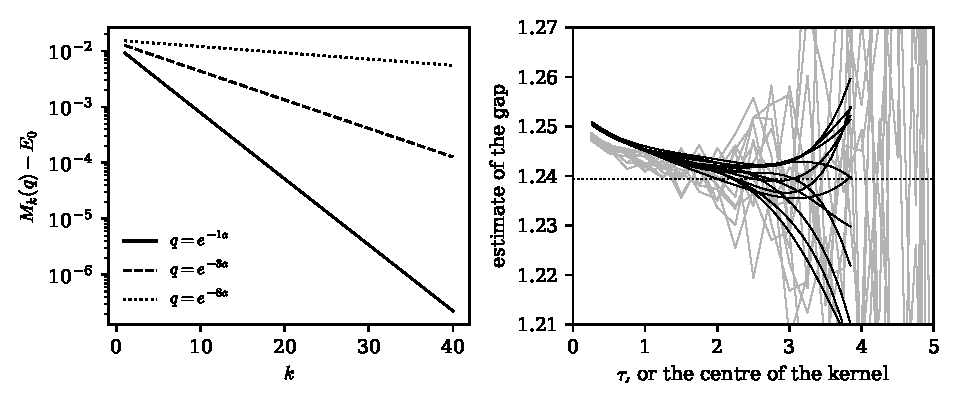
\includegraphics[width=\textwidth]{figures/window_gap.pdf}
\caption[A monotone estimator of the gap]{Left: the excess of $M_k(q)$ over the gap for the exact correlator, for three values of $q$; it is positive and decreasing, as Proposition~\ref{prop:windowgap} says. Right: twelve noisy replicates of the effective mass (grey) and of $M_k$ with $q=e^{-3a}$ (black) against the time at which the kernel is centred; the dotted line is the gap.}
\label{fig:windowgap}
\end{figure}

At matched bias the kernel estimator has about half the noise of the effective mass at short times, a little less at moderate times, and more at long times, where its kernel reaches into the region in which the signal is below the noise. So it is a modest tool with one real merit: every $M_k$ is a rigorous upper bound for the gap, and the sequence is monotone, whatever the spectrum.

\paragraph{\normalfont\scshape Why the kernels are the same.} The localising kernel $u^ke^{-\sigma u}/k!$ of \cite{DLCL} is, after normalisation, the density of a gamma variable of shape $k+1$, the kernel of the inversion formula of Post and Widder~\cite{Pt30,Wi41}, and the negative binomial weight $\binom{j+k}{k}q^j$ is its lattice form: the law of the number of failures before the $(k+1)$st success. Both are convolution powers of one law, exponential or geometric, and both concentrate at relative width $k^{-1/2}$. In the language of this book the first is the simplest generalized gamma convolution and the second its lattice analogue, and the estimator $M_k$ is a ratio of two expectations of the correlator under them. The edge of the support of a positive measure is the limit of ratios of its moments.

\paragraph{\normalfont\scshape A positive selector.} In \cite{DLCL} the functions for different characters are combined with strictly positive coefficients, so that a zero of any one of them is a pole of the sum and cannot cancel. The same device is available here and is equally cheap: a positive combination of reflection positive correlators over channels, for instance $\sum_nc_n\langle\chi_n(U_p)(0)\,\chi_n(U_p)(\tau)\rangle$ with $c_n>0$, has a spectral measure that is the sum of those of its terms, and its gap is the smallest of theirs.

\paragraph{\normalfont\scshape Frames and mean slopes.} The third mechanism is the one the account marks as specific to the construction. There are many maps $J_i$ from small hermitian lattices into one large one, and what is needed is that their images, taken together, fill the target. The step in finite dimensions is the following. It is stated and proved in the exposition \cite{Rub26} of the next section (Part II, section 6.9); we give the proof because it is short and contains no arithmetic. Write $\|A\|_2^2=\operatorname{tr}(A^*A)$.\index{frame lemma}

\begin{lemma}[frame lemma]\label{lem:frame}
Let $J_i:V_i\to H$ be linear maps of complex inner product spaces of finite dimension, with $D=\dim H$ and $W=\sum_i\dim V_i$, and let $c_i>0$. Put $K_i=c_iJ_i^*J_i$ on $V_i$ and $Q=\sum_ic_iJ_iJ_i^*$ on $H$. Then
\[
\operatorname{rank}Q\ \ge\ \frac{(\operatorname{tr}Q)^2}{\operatorname{tr}(Q^2)}.
\]
Suppose further that
\[
\sum_i\|K_i-1\|_2^2\le eW,\qquad e\le\tfrac14,\qquad\operatorname{tr}(Q^2)\le(1+\eta)\,\frac{(\operatorname{tr}Q)^2}{D},
\]
and let $U_i\subset V_i$ be subspaces with $\sum_i(\dim V_i-\dim U_i)\le\alpha W$. Then
\[
\operatorname{codim}\sum_iJ_iU_i\ \le\ \big(\eta+4\alpha+4\sqrt e\,\big)D.
\]
\end{lemma}

\begin{proof}
The first statement is the Cauchy and Schwarz inequality for the nonzero eigenvalues of $Q$. For the second we may take $\alpha\le1$. Let $P$ be the orthogonal projection of $H$ onto the complement of $\sum_iJ_iU_i$, of dimension $zD$. The operator $A_i=c_iJ_i^*PJ_i$ is nonnegative, is at most $K_i$, and vanishes on $U_i$. So with $R_i$ the projection of $V_i$ onto the complement of $U_i$, of rank $r_i$,
\[
\operatorname{tr}A_i=\operatorname{tr}(R_iA_i)\le\operatorname{tr}(R_iK_i)=r_i+\operatorname{tr}\big(R_i(K_i-1)\big)\le r_i+\sqrt{r_i}\,\|K_i-1\|_2.
\]
Summing, and using the Cauchy and Schwarz inequality over $i$,
\[
\operatorname{tr}(PQ)=\sum_i\operatorname{tr}A_i\le\big(\alpha+\sqrt{\alpha e}\,\big)W,
\]
\[
\operatorname{tr}Q=\sum_i\operatorname{tr}K_i\ge\big(1-\sqrt e\,\big)W\ge\tfrac12W.
\]
Let $\bar q=\operatorname{tr}Q/D$. The hypothesis on the second moment says $\|Q-\bar q\|_2^2\le\eta(\operatorname{tr}Q)^2/D$, so
\[
\operatorname{tr}(PQ)=\bar q\,zD+\operatorname{tr}\big(P(Q-\bar q)\big)\ge\big(z-\sqrt{\eta z}\,\big)\operatorname{tr}Q.
\]
Dividing by $\operatorname{tr}Q$ and using $\sqrt{\eta z}\le\frac12(\eta+z)$ gives $z\le2\alpha+2\sqrt e+\frac12(\eta+z)$, which is the claim.
\end{proof}

The two hypotheses say that the maps form an approximate tight frame: each $c_iJ_i^*J_i$ is close to the identity on average, and the frame operator $Q$ is close to a scalar in mean square. The conclusion is a pooled local to global principle. What holds on most of each piece holds on most of the whole. Two maps onto the two axes of $\mathbb C^2$ have $Q=1$ and fill the plane; two maps onto the same axis have the same trace, twice the second moment, and fill a line.

The constants can be improved, and the improved form is sharp.

\begin{proposition}[sharp form]\label{prop:framesharp}
In Lemma~\ref{lem:frame} assume only $e<1$, and put $\rho=(\alpha+\sqrt{\alpha e}\,)/(1-\sqrt e\,)$. Then
\[
\operatorname{codim}\sum_iJ_iU_i\ \le\ \tfrac14\Big(\sqrt\eta+\sqrt{\eta+4\rho}\,\Big)^2D\ \le\ (\eta+2\rho)\,D.
\]
For a tight frame of isometries, $e=\eta=0$, the bound is $\alpha D$, and it is attained.
\end{proposition}

\begin{proof}
The proof of the lemma gives $z-\sqrt{\eta z}\le\operatorname{tr}(PQ)/\operatorname{tr}Q\le\rho$, a quadratic inequality in $\sqrt z$ whose solution is the first bound; the second follows from $\sqrt{\eta^2/4+\eta\rho}\le\eta/2+\rho$. For $e\le\frac14$ and $\alpha\le1$ one has $2\rho\le4\alpha+4\sqrt e$, which recovers the lemma. An orthogonal decomposition $H=\bigoplus_iV_i$ with the inclusions as maps is a tight frame of isometries with $W=D$, and removing a proportion $\alpha$ of the directions of the pieces removes exactly $\alpha D$ directions of $H$.
\end{proof}

In random trials (\texttt{frame\_lemma.py}), $270$ configurations with up to eight maps into spaces of dimension up to forty, neither bound was violated. The lemma as stated says something, a bound below $D$, in $23$ of them, and the sharp form in $58$.

The second step turns a count of directions into a bound for an average.

\begin{corollary}[few low states]\label{cor:lowstates}
Under the hypotheses of Lemma~\ref{lem:frame} on $J_i$, $c_i$, $e$ and $\eta$, let $T$ be a self adjoint operator on $H$ with $T\ge a-L$, where $L\ge0$. Suppose that for each $y\in[0,L]$ there are subspaces $U_i(y)\subset V_i$, of total codimension at most $\alpha(y)W$, with $\langle Tw,w\rangle\ge(a-y)|w|^2$ for every $w$ in $\sum_iJ_iU_i(y)$. Then the number $N(y)$ of eigenvalues of $T$ below $a-y$ is at most $(\eta+4\alpha(y)+4\sqrt e\,)D$, and
\[
\frac{\operatorname{tr}T}{D}\ \ge\ a-\big(\eta+4\sqrt e\,\big)L-4\int_0^L\alpha(y)\,dy.
\]
\end{corollary}

\begin{proof}
If $T\ge\lambda$ on a subspace of codimension $r$ then $T$ has at most $r$ eigenvalues below $\lambda$, since the span of more than $r$ such eigenvectors would meet the subspace. With the lemma this bounds $N(y)$. For the mean, with eigenvalues $\lambda_j$,
\[
\frac{\operatorname{tr}T}{D}\ \ge\ a-\frac1D\sum_j(a-\lambda_j)_+=a-\int_0^L\frac{N(y)}{D}\,dy,
\]
the layer cake formula.
\end{proof}

In \cite{Rub26} the function $\alpha$ comes from Markov's inequality: if numbers with mean at least $s$ are all at most $s+u$, the proportion of them below $s-y$ is at most $u/(u+y)$. Then $4\int_0^L\alpha=4u\log(1+L/u)$, a logarithmic loss in the spread $u$, and the mean slope of the sources is carried to the target. There the operator is a slope and its filtration is that of Harder and Narasimhan~\cite{HN75}; that filtration is what makes a bound on each image a bound on their sum, and the draft says it takes it from the Lean development.

It is fair to say what this would and would not give here. The corollary bounds $\operatorname{tr}T/D$, an average over the spectrum: with $T$ the logarithm of a transfer matrix on a finite block this is a free energy, and for loops a string tension, a rate per unit area. A gap is a statement about the bottom of the spectrum, a set of relative dimension zero, and a bound that allows a small proportion of exceptions cannot see it. So the frame mechanism is a candidate for transferring string tensions under blocking, where the sandwich of Chapter~\ref{ch:sandwich} asks for exactly a comparison of averaged rates, and not for the gap itself. The hypothesis that carries the weight is the form bound on the sum $\sum_iJ_iU_i(y)$, which involves cross terms between the pieces. For blocks of a lattice we do not know what supplies it, and we have not tried.

\paragraph{\normalfont\scshape The budget.} The exponent $\frac12$ comes out in \cite{DLCL} as a balance between a gain repeated along a tower of length $m$ and costs that grow with $m$ in another way. The next section gives its explicit form and the form it takes for the ladder.

We read sections 1, 2 and 5 of \cite{DLCL} in full and part of section 6, and only the headings of the rest; the copy we read names no author. Its arithmetic is taken as stated.

\section{The inequality (M) and the three scales}\label{sec:ineqM}\index{inequality (M)}\index{Chebyshev, P. L.}

The argument for the zeta function alone is set out in a working draft written at the behest of M. O. Rubinstein \cite{Rub26}, which our deck \cite{PS26m} follows. It reduces the Riemann hypothesis to three inputs, and it is explicit about which of them it proves. The statistic is a smoothed Chebyshev sum with its main term removed,
\[
G(x)=\sum_{n\le x}\Lambda_{\mathrm{vM}}(n)\Big(\frac xn-1\Big)-x\log x+(1+\gamma_E)x
=\log2\pi-\sum_{\varrho}\frac{x^{\varrho}}{\varrho(\varrho-1)}+O(x^{-2}),
\]
the sum being over the zeros in the strip, and the criterion is the one sided window of the last section: if $G(x)\le x^{1/2+\varepsilon}$ on intervals $[Y,Y^{3/2}]$ with $Y$ arbitrarily large, there is no zero to the right of the critical line. Two auxiliary primes $q$ and $d$ give the combination $(1+\chi_q)(1-\chi_d)$, whose weight $1-\chi_d$ is nonnegative and selects the primes inert in $\mathbb Q(\sqrt{-d})$. Then:
\begin{itemize}
\item Estimate B, at the scale $x$, far below the conductors: square root bounds for the three twisted sums;
\item Estimate C, at scales far above the conductors: bounds with an exponential saving, from the classical zero free region, for the characters of the table of cells;
\item the inequality (M), an averaged one sided comparison of a prime sum $P$ with nonnegative weights, cut off cell by cell, against its main term $M$, with $B$ the bound of Estimate B,
\[
\frac1n\sum_{u\in H}\sum_{v\in T}\sum_{j\le m}\big(P_{u,v,j}-M_{u,v,j}\big)\le E,
\]
\[
\frac EB\le x^{c_0\varepsilon}\Big(\frac xm+\frac{xm}{k}+m+\frac{k}{n^2}\Big),
\]
with $c_0$ a constant fixed in the draft;
\end{itemize}
B and C are proved in the draft from published theorems on Dirichlet $L$ functions. The inequality (M) is not: the draft proves parts of it, proves others conditionally on named statements, and says it takes the rest from the Lean development. In the table of cells behind (M) a small proportion of distinguished cells tests the primes at the scale $x$ and carries the main term, and every other cell sits at a scale so large that Estimate C makes it negligible.

\paragraph{\normalfont\scshape Divisibility against size.} The source of every upper bound in the argument is Chebyshev's: a nonzero integer divisible by $p^{e_p}$ for each $p$ is at least $\prod p^{e_p}$. For the middle binomial coefficient this bounds the primes between $n$ and $2n$, and it stalls at constants because the exponents of a factorial are floor functions. The draft replaces the integer by a linear map $T:L\to M$ between lattices. If $T$ is injective and $T(L)\subset p^eM$ then
\[
e\log p\ \le\ \log\|T\|+\mu_{\max}(M)-\mu(L),
\]
where the slope $\mu$ of a lattice is minus the logarithm of its covolume divided by its rank, and $\mu_{\max}(M)$ is the largest slope of a nonzero sublattice of $M$; for $L=M=\mathbb Z$ this is Chebyshev's inequality. The maps are theta lifts between definite unitary groups, which are matrices of derivatives of theta functions. At an inert prime a derivative of order $a$ is divisible to the smooth exponent $a(1/p+1/p^3+\cdots)$, with no floor function, and its squared size is that of the Gaussian integral $\|z^a\|^2=a!$. The two sides, summed over the primes, then agree to leading order $a\log a$, and (M) is the statement that they agree in the term linear in $a$ as well, up to $E$.

\paragraph{\normalfont\scshape The budget.} The four terms have different origins (\cite{Rub26}, section I.8). The term $x/m$ collects errors made once, in the sizes of the lattices at the two ends of a chain of $m$ lifts: the gain from divisibility is collected $m$ times, so they are divided by $m$. The term $m$ collects errors made at every step. The terms $xm/k$ and $k/n^2$ are the costs of a rank $k$ and of the size $n$ of the table. With $m=x^{1/2}$, $k=x^{9/2}$ and $n=x^2$, up to powers of $x^\varepsilon$, the terms are $x^{1/2}$, $x^{-3}$, $x^{1/2}$ and $x^{1/2}$. That is why the exponent is one half. Had the errors of the steps cost $m^2$ after normalisation, the balance of $x/m$ against $m^2$ at $m=x^{1/3}$ would give only the half plane to the right of $\frac23$; the precision of the comparison of lattices decides the exponent.

We have read Part I of the draft, the sections of Part II on slopes and ranks, and the table of what Part III proves; we have not read the proofs of Part III. With that said, the architecture resembles what one would expect of a proof of the mass gap, and the correspondence is close enough to set out.

\begin{center}
\small
\begin{tabular}{p{0.46\textwidth}p{0.46\textwidth}}
\toprule
the argument through (M) & the mass gap \\ \midrule
Estimate B: below the conductor the characters behave like random signs, square root cancellation & weak coupling at short scales: asymptotic freedom, the renormalisation group of Ba\l aban \cite{Ba87}, the first rungs of the ladder \\
Estimate C: far above the conductor a classical zero free region gives an exponential saving & strong coupling at long scales: the convergent expansion of Osterwalder and Seiler \cite{OSe} gives an area law and a gap \\
(M): the bridge between the two scales, one sided and averaged & the comparison at intermediate coupling, Chapter~\ref{ch:sandwich} \\
the one danger in C is an exceptional real zero, avoided by the choice of $q$ and $d$ & the one danger is a phase transition at intermediate coupling; on the projected ladder Corollary~\ref{cor:contracts} excludes it \\
nonnegative weights $1-\chi_d$ & the nonnegative action $1-\frac12\operatorname{tr}U=2\sin^2(\theta/2)$ and reflection positivity \\
distinguished cells carry the main term, the rest are killed by C & blocks at the scale of the correlation length carry the gap, coarser ones are in the strong coupling phase \\
budget $x/m+xm/k+m+k/n^2$, balanced at $x^{1/2}$ & a drift per rung against an error per rung (below, and Open problem~\ref{op:slopes}) \\
(M) is, by the draft, taken in part from the Lean development & existence is quoted from an announced proof, not checked by us (Section~\ref{sec:existence2026}) \\
\bottomrule
\end{tabular}
\end{center}

Two things in this are more than analogy. The first is the logic. Both ends of the scale are classical in both problems, and in both the whole difficulty is a one sided inequality across the middle. Proposition~\ref{prop:windowgap} says that for the gap one sidedness and sparseness are free, so the statement to prove has the following form.

\begin{problem}[an inequality of type (M) for the ladder]\label{op:MYM}
For SU(2) lattice gauge theory in four dimensions at coupling $\beta$, let $c_n$ be the count $E[1/(1-\frac12\operatorname{tr}U)]-2$ of the plaquette of the lattice blocked $n$ times with scale factor $2$, and $\ell_n$ the count after $n$ exact rungs of the ladder from the law of the fine plaquette. Prove $c_n\le\ell_n+E_n$ with an error $E_n$ small enough that $\ell_n+E_n$ still falls below the threshold of the strong coupling expansion after a number of blockings proportional to $\beta$. Only an upper bound is asked, and only along the sequence of scales $2^n$.
\end{problem}

\paragraph{\normalfont\scshape The budget of the ladder.} The ladder has the same two kinds of error and a different arithmetic. Suppose that $c_n\le\ell_n+e_0+e_1n$, with an error $e_0$ made once and an error $e_1$ made at every rung, and that the count on the ladder falls by $\delta$ per rung, $\ell_n\le\ell_0-\delta n$. Then
\[
c_n\le c_*\qquad\text{as soon as}\qquad n\ \ge\ \frac{\ell_0-c_*+e_0}{\delta-e_1}.
\]
In (M) the gain grows with the length of the chain and is set against costs that grow too, and the optimum is interior. Here the gain is a fixed drift, so there is no optimum and one condition: $e_1<\delta$, the error per rung must be smaller than the drift. An error made once costs $e_0/(\delta-e_1)$ further rungs, a fixed factor in the scale, and is harmless.

The numbers at weak coupling are these. The plaquette of the four dimensional lattice has $1-\langle\frac12\operatorname{tr}U_p\rangle=3/(4\beta)$ to leading order, and its field strength is Gaussian in three components, for which $E[1/(1-x)]=3/E[1-x]$. So $\ell_0=c_0=4\beta$ to leading order, twice the count $2\beta-\frac32$ of a Wilson law at the bare coupling: the plaquette in four dimensions is stiffer than its action alone would make it. The drift is $\delta=\frac12$, a numerical observation for heat kernels (Theorem~\ref{thm:firstrung} proves the first rung only for point masses and Wilson laws, and the limit $r\to\frac13$ that gives $\frac12$ is unproved). With no error the ladder from the fine plaquette therefore needs about $8\beta$ rungs, a scale $2^{8\beta}=e^{5.55\beta}$, while asymptotic freedom puts the correlation length at $e^{3\pi^2\beta/11}=e^{2.69\beta}$ up to a power of $\beta$, about $3.9\beta$ blockings. So $c_n\le\ell_n$ has room at weak coupling: the true count must fall about twice as fast as the ladder's, and $e_1$ may be taken negative. The ladder from the bare Wilson law, by contrast, needs $4\beta$ rungs against $3.9\beta$, the agreement of the decrement $\frac14$ with $0.26$ noted in Chapter~\ref{ch:sandwich}; but its count starts below $c_0$, and the inequality fails for it at $n=0$.

Two cautions belong with these numbers. The leading order is not yet accurate at the couplings we can simulate: at $\beta=2.3$, $2.5$ and $2.7$ the measured $E[1/(1-x)]$ is $7.2$, $8.3$ and $9.2$ against $4\beta=9.2$, $10.0$ and $10.8$, a ratio that rises from $0.78$ to $0.85$. And the comparison of $8\beta$ with $3.9\beta$ is a comparison of exponents only. It says that the ladder from the fine plaquette reaches strong coupling at a scale near the square of the true one, which is the direction an upper bound must err in, and it says nothing about any finite $n$.

\begin{center}
\small
\begin{tabular}{lccc}
\toprule
 & start & blockings & scale \\ \midrule
ladder from fine plaquette & $4\beta$ & $8\beta$ & $e^{5.55\beta}$ \\
ladder from bare Wilson law & $2\beta$ & $4\beta$ & $e^{2.77\beta}$ \\
asymptotic freedom & & $3.9\beta$ & $e^{2.69\beta}$ \\
\bottomrule
\end{tabular}
\end{center}

The evidence is in Tables~\ref{tab:countblocked} and~\ref{tab:countblocked2}, where the ladder starts from the Wilson law matched to the fine plaquette rather than from the law of the fine plaquette itself. On $16^4$ with two blockings $c_n\le\ell_n$ holds at both levels for $\beta=2.3$ and $2.5$, with a margin that grows with the level, $1.27$ against $4.87$ and $4.00$ against $6.04$ at the second. At $\beta=2.7$ it fails at the first level, $8.14$ against $7.48$, and holds at the second, $6.75$ against $7.01$: a smeared blocking at weak coupling first raises the count. In the terms above that is an error $e_0$ of about $0.7$ made once, and between the first and second levels the lattice count falls by $2.5$, $2.1$ and $1.4$ at the three couplings against $0.47$ on the ladder, so $e_1$ is negative there. This is two rungs on small lattices; it is not an estimate of either error.

The second is the device of averaging. In (M) the average over the translates $u\in H$ is what turns the selection of cells into characters, by orthogonality on a cyclic group. The lattice has the same device with the gauge group in place of $H$: averaging over gauge transformations is what turns products of link variables into characters of plaquettes, and it is how the matching expansion of Theorem~\ref{thm:matching} was obtained. A proof of Open problem~\ref{op:MYM} would presumably use it in the same way, to replace the blocked measure by an average of measures each of which is a product over cells.

\section{What theta lifts do not give}

The engine of the chain is arithmetic: divisibility of theta values at inert primes, a slope inequality that trades it against archimedean size, and the balance of the two that fixes the length of the chain. Yang Mills has none of this. The step that turns a one sided bound into a zero free region needs a Dirichlet series with positive coefficients; the mass gap needs a spectral bound for an operator in infinitely many variables. Induced gauge theories built from flavours change the action, and whether they lie in the universality class of Yang Mills is open by their authors' own account. And everything in this chapter concerns one plaquette or one decimation: the lattice $\mathbb Z^4$ is untouched.

It helps to be exact about where the proof of (M) lives. By the account of \cite{Rub26}, three things have to be established about the lifts: divisibility at inert primes, which rests on the integrality of the theta kernels in the coordinates of a formal group of height two; size to the precision of the linear term, which rests on the inner product formula, the formula of Chowla and Selberg and the mass formula; and control of denominators and of rank, which rests on a bound for Galois cohomology and on a relative trace formula. All of that is arithmetic, none of it has a counterpart for a lattice gauge theory, and the draft says it takes the parts it does not prove from the Lean development. What transfers is what surrounds it: the one sided window, the frame lemma, the passage from a count to a mean, and the shape of the budget. Those are the four things this chapter has taken.

\section{Open problems}

\begin{problem}\label{op:matching}
Prove that the matching expansion of Theorem~\ref{thm:matching} has only real zeros in $x$, all at most $-1$, for hopping parameters in $(0,1]$: a theorem of Heilmann and Lieb type for the variable that marks only the pairs between two blocks of a complete graph. This is Conjecture~\ref{conj:Lclosed}.
\end{problem}

\begin{problem}\label{op:symplectic}
Write the colour flavour transformation for SU(2) as a symplectic group, with the inner pairs, and identify the law of the masses $\lambda_i(Z)$ of the mixture. For all hopping parameters equal to $1$ the answer is the hypergeometric law of the count.
\end{problem}

\begin{problem}\label{op:slopes}
Bound the error per rung $e_1$ of Section~\ref{sec:ineqM} below the drift $\frac12$ of the count, for some blocking of the four dimensional lattice and all $\beta$ large. By the budget of the ladder this, with any bound on the error $e_0$ made once and the drift $\frac12$ at every rung (a numerical observation, with the first rung theorem covering only point masses and Wilson laws), would give Open problem~\ref{op:MYM}. At weak coupling the true count falls about twice as fast as the ladder's, so the bound is expected with room to spare; nothing is proved.
\end{problem}

\section{Assessment}

Useful, as a language and for one open problem. The determinant form explains why the class $\mathcal L$ is natural, why the count is a sum of Bernoulli variables and why the heat kernel belongs to it. The matching expansion is a new exact formula for decimation and brings the closure conjecture within sight of a classical theorem, separated from it by the pairs inside each law. The window criterion of the expanded account becomes, for a positive spectral measure, an elementary proposition and a monotone estimator of the gap. The frame lemma is portable as it stands and bounds averages, not gaps. The budget of (M) becomes one condition for the ladder, an error per rung below the drift. Nothing here is a step toward the gap on $\mathbb Z^4$. We read \cite{PS26t} in full; its account of the arithmetic of the chain is taken from the sources it cites, and so is ours. The colour flavour formula above is quoted from memory of \cite{Zi96} and checked in one case only.

\section*{Exercises}
\begin{enumerate}
\item (Section~\ref{sec:t11det}) Verify $\det(1+\alpha U)=(1-\alpha)^2+\alpha\det(1+U)$ and deduce the Bernoulli parameter $1/\gamma$ of the count from the normalisations $Z_0=1$ and $Z_1=1$.
\item (Section~\ref{sec:t11howe}) From Proposition~\ref{prop:howe} show that $a_1=\sum_qe_q^2-\sum_qe_qe_{q+2}$ and compute it for $\alpha=(1,1)$.
\item (Section~\ref{sec:t11match}) List the matchings of four flavours, two in each law, and recover $f_2*f_2$ from Theorem~\ref{thm:matching}.
\item (Section~\ref{sec:windows}) Prove Proposition~\ref{prop:windowgap}(ii) for a spectral measure with two atoms, and find the rate at which $M_k(q)$ approaches $E_0$ in terms of $q$ and the two energies. Which $q$ makes the approach fastest, and why is that choice useless with noisy data?
\item (Section~\ref{sec:windows}) Prove that $\operatorname{rank}Q\ge(\operatorname{tr}Q)^2/\operatorname{tr}(Q^2)$ for a nonnegative matrix $Q$, and find $\eta$ in Lemma~\ref{lem:frame} for $p$ isometries of $\mathbb C^r$ into $\mathbb C^D$ with orthogonal images and $c_i=1$. When does the lemma say the images fill the target?
\item (Section~\ref{sec:windows}) For numbers with mean at least $s$ and maximum at most $s+u$, show that the proportion below $s-y$ is at most $u/(u+y)$, and that this cannot be improved.
\item (Section~\ref{sec:ineqM}) In the budget of the ladder take $\ell_0=4\beta$, $c_*=1$ and $\delta=\frac12$. For which $e_1$ does the number of rungs equal the $3.9\beta$ blockings of asymptotic freedom at large $\beta$? What does the sign of the answer say about the ladder?
\item (Section~\ref{sec:t11match}) Show that for U(2) the average of $\det(1+\alpha UV^{-1})\det(1+\kappa V)$ over $V$ is $1+\alpha\kappa x+\alpha^2\kappa^2$ for $U$ in SU(2), and compare with the SU(2) convolution. Which terms are the inner pairs?
\end{enumerate}

\part{Open Problems}
\chapter{A Path to the Mass Gap}\label{ch:path}

Chapter~\ref{ch:theta} completed the toolkit. This chapter opens Part V, on the open problems. It assembles the pieces into a programme, separates what is done from what is not, and describes the idea we would try first on the rest. The first sections list the stages of the path and the open problems; Section~\ref{ch:isthere} states the mass gap conjecture in Thorin form and weighs the routes to the missing step; Section~\ref{ch:missing} lists ideas we have not used and recent work of others; Section~\ref{ch:threed} makes the case for attempting three dimensions first.

\section{The five stages}

\begin{enumerate}
\item[(i)] Positivity at every scale. Done for the lattice theory and for the Migdal Kadanoff rungs, not shown for a block spin transformation of the true flow. Reflection positivity on the lattice (Chapter~\ref{ch:positivity}), the preservation of nonnegative character coefficients at every Migdal Kadanoff rung (Lemma~\ref{lem:posB}), and the equivalence theorem (Theorem~\ref{thm:equivB}), which turns a uniform gap into a uniform inequality between positive Thorin densities with constant one.
\item[(ii)] Strong coupling. Done. The Osterwalder and Seiler cluster expansion~\cite{OSe} gives a positive lattice mass for $\beta<\beta_0$ (Chapter~\ref{ch:strong}), as does the log Sobolev argument of Shen, Zhu and Zhu~\cite{SZZ}.
\item[(iii)] The renormalization ladder in the Migdal Kadanoff approximation. Partly done. The asymptotics (Remarks~\ref{prop:decrementB} and~\ref{prop:sunB}), the monotonicity (Lemma~\ref{lem:mlrB}) and the covering on $[0.3,300]$ (Remark~\ref{prop:coverB}) are in place. The likelihood ratio hypothesis of the lemma is now a theorem (Corollary~\ref{cor:mlrall}). The decrement inequality for the heat kernel projected map is now Corollary~\ref{cor:contracts}; for the exact ladder the decimation half is open. Chapter~\ref{ch:strong} proves the first passage criterion for the projected map only. A computer assisted gap theorem for the Migdal Kadanoff hierarchical lattice, with asymptotic freedom scaling and an explicit coefficient, would follow if three things were added, each still open: a proof that the projected map controls the exact hierarchical recursion, a strong coupling mass with explicit constants, and boundedness in physical units (conditions (C), (D) and (E) of that chapter, where (E) fails as stated for the ladder and must be replaced), together with interval arithmetic and an explicit remainder for the rate. Confinement on hierarchical lattices of this type was proved by Ito in 1985~\cite{Ito85}; the new content would be the quantitative spectral statement and the identification of the coefficient as $(1-b^{-2})\E S_{\mathrm{BPY}}$.
\item[(iv)] Comparison with $\Z^4$. Open. The true renormalization flow must be bracketed between Migdal Kadanoff type flows strongly enough that the decrement inequality, or the uniform Thorin gap inequality, passes from the bracketing flows to the true one.
\item[(v)] The continuum theory. Announced, not independently checked. OpenAI announced on 26 October 2026 a proof, with a Lean formalisation, of the existence of certain four dimensional gauge theories including pure Yang Mills~\cite{OAI}; a review group led by D. Gross endorsed the existence part on 9 November. It is not refereed, and Woit disputes it as a weak existence result obtained by compactness~\cite{Woit26}. The announcement does not claim the mass gap. If the result is sustained it would supply a continuum theory, which is what this stage assumes. Ba\l aban's renormalization group~\cite{Ba87} controls the ultraviolet, and Magnen, Rivasseau and S\'eneor constructed SU(2) Yang Mills in finite volume~\cite{MRS}. What stage (v) still needs from us is the identification of the continuum spectral measures as weak limits of the lattice ones, so that Corollary~\ref{cor:continuumB} applies.
\end{enumerate}

Even if stage (iv) were established, stage (iii) would still need its remainder and its conditions, and stage (v) its identification of limits. Stage (iv) is where a new idea is needed.

\section{Why the comparison is hard}

Kadanoff's original argument~\cite{Ka75,Ka76} shows that bond moving\index{bond moving} gives one sided inequalities for free energies: moving bonds in one direction raises the free energy and in the other lowers it. Tomboulis\index{Tomboulis, E. T.}, in 2007~\cite{To07}, tried to use such inequalities to bracket the partition functions of the true theory in the presence of a centre vortex flux between those of Migdal Kadanoff\index{Migdal Kadanoff recursion} type flows, as a route to confinement\index{confinement} at all couplings. Ito\index{Ito, K. R.} and Seiler pointed out missing links in the argument, in a note of November 2007 and a longer discussion of March 2008~\cite{IS}, and Seiler gave a further critical discussion at the Confinement VIII conference~\cite{Se12}. The argument is not accepted as a proof.

The difficulty, in the language of this book, is a mismatch of objects. Free energies are logarithms of partition functions, one number per volume. The gap is a property of spectral measure\index{spectral measure}s, which are infinite dimensional. A bracket on free energies controls the spectral measures only through their total mass, and says nothing about where they are supported. The equivalence theorem tells us exactly what must be bracketed instead: the family of Thorin densities, or equivalently the correlations at all Euclidean times, uniformly in the lattice spacing.

\section{A probabilistic sandwich}

\begin{problem}[Thorin sandwich]\label{op:sandwichB}
Construct maps $R_-\le R_+$ on positive definite class functions, of Migdal Kadanoff type, whose flows bracket the true four dimensional spectral measures in the sense of the uniform Thorin gap inequality. Then prove the decrement inequality for $R_-$.
\end{problem}

The ordering $R_-\le R_+$ needs a meaning, with larger meaning more disordered, that is stronger coupling. The verification of Section~\ref{ch:verification} suggests one: the likelihood ratio\index{likelihood ratio order} order on laws of the rotation angle, which drove the monotonicity of $R$. Our proposal for attacking the problem has three steps.

First, realise the true block spin transformation of lattice gauge theory and the Migdal Kadanoff step on a common probability space. Both act on random group elements: the true transformation integrates out interior links of a block with their exact conditional law, and the Migdal Kadanoff step replaces that conditional law by a product of independent copies followed by a convolution. Brownian motion\index{Brownian motion on SU(2)}s on SU(2) supply a natural common space, because the heat kernel\index{heat kernel} laws are the fixed forms of decimation\index{decimation}.

Second, compare the resulting laws of the block holonomy in the likelihood ratio order. The tools are those of Section~\ref{ch:toolkit}: likelihood ratio orders are preserved by products and by convolution with log concave kernels, which are exactly the two Migdal Kadanoff operations.

Third, control the failure of log concavity. On a flat space the Gaussian laws are log concave and the argument would close. On SU(2) the Haar density $\sin^2\theta$ and the curvature factor $\theta/\sin\theta$ break log concavity away from the identity. Positive curvature helps some inequalities: the Riemannian Pr\'ekopa Leindler (Borell Brascamp Lieb) inequality of Cordero Erausquin, McCann and Schmuckenschl\"ager~\cite{CMS} holds on manifolds with Ricci curvature bounded below, and the Bakry \'Emery curvature dimension calculus~\cite{BE} gives functional inequalities for heat flow. Neither states that geodesic log concavity is preserved by heat flow or by marginalisation, and on the compact three sphere it could not be the right notion for laws spread over the group: a geodesically log concave function on the whole group is constant, as one sees by restricting it to a closed great circle. So at the crossover, where the laws are spread over the whole group, a substitute for geodesic log concavity is needed, and finding one is the concrete question. Chapter~\ref{ch:progress} adds one fact: in the variable $c=\cos\theta$ the heat kernel, and every power of it, is log concave on $[-1,1]$ (Corollary~\ref{cor:logconc}). The Haar weight $\sqrt{1-c^2}$ is also log concave in $c$, so the law of $c$ is log concave. The failure of log concavity is therefore a feature of the angle coordinate, and whether the likelihood ratio comparison can be carried out in the coordinate $c$ is open.

\section{Block spin transformations}

To make stage (iv) concrete we need a definition of the true renormalization step on $\Z^4$. The classical choice, used by Ba\l aban\index{Balaban, T.@Ba\l aban, T.}, is a block spin transformation. The lattice is partitioned into blocks of side $b$; for each pair of neighbouring blocks a new link variable is defined as an average of the products of original links along the paths that connect the block centres; and the new measure is the conditional law of these averaged variables, or a smoothed version of it with a Gaussian like kernel that keeps it concentrated near the average. Gauge invariance is preserved because the averaging is covariant.

Three features of this construction matter for a probabilistic comparison.
\begin{enumerate}
\item[(i)] The new link variables are functions of many old ones, and the new plaquette weight is no longer a function of single plaquettes: the effective action contains larger loops. Migdal Kadanoff truncates these to single plaquettes. A comparison must control the truncated terms, or show that they enter with a definite sign in the relevant order.
\item[(ii)] At weak coupling the block spin conditional laws are close to Gaussian on the Lie algebra, with corrections controlled by perturbation theory. In this regime Ba\l aban's bounds are available, and the comparison with Migdal Kadanoff should reduce to a comparison of the curvature corrections, which Section~\ref{ch:mk} expresses through the Biane Pitman Yor variable~\cite{BPY}.
\item[(iii)] At the crossover the laws spread over the whole group and no expansion applies. This is where the likelihood ratio and curvature tools must do their work, and where the positivity preserved at every rung (Lemma~\ref{lem:posB}) is essential, since it is the only structure that survives without an expansion.
\end{enumerate}

\section{A check in two and three dimensions}

In two dimensions Migdal Kadanoff is exact, because bond moving is trivial when $d-2=0$, and the comparison of stage (iv) holds with equality. The two dimensional theorem of Chapter~\ref{ch:twod} is therefore the complete version of the programme in that dimension. In three dimensions the coupling has dimension of mass, the theory is superrenormalizable, and Remark~\ref{prop:decrementB} shows that the precision falls by a factor $b$ per step even in flat space. There the gap is expected to follow from the dimensional running alone, and the curvature correction is subleading. A full comparison in three dimensions, between the Migdal Kadanoff ladder and the true lattice theory, would be a natural intermediate goal before four dimensions, and would test the probabilistic sandwich where the analytic stakes are lower.

\section{What a proof would have to contain}

It is useful to list what a complete argument along these lines would have to contain, so that progress can be measured.
\begin{enumerate}
\item A precise block spin transformation on $\Z^4$ for which the true flow is defined at every scale, together with reflection positivity at every scale.
\item Two Migdal Kadanoff type maps and a proof that they bracket the true flow in an order strong enough to control spectral measures.
\item A computer assisted proof of the decrement inequality for the lower map on a compact range of couplings, joined to the cluster expansion at strong coupling and to the asymptotic analysis at weak coupling (which needs an explicit remainder).
\item An identification of the continuum spectral measures with weak limits of the lattice ones, and an application of the continuum corollary.
\end{enumerate}
None of the four is done. Item 1 needs reflection positivity at every scale for the block spin transformation, for which we have no argument: Lemma~\ref{lem:posB} preserves nonnegative character coefficients at the Migdal Kadanoff rungs and does not give reflection positivity for the true flow. Item 3 presupposes the lower map of item 2, which does not yet exist. Item 4 is the identification of stage (v), still to be done. Item 2, the bracketing, is stage (iv) and is the problem.

\section{Open problems}

We collect the open problems of the book, in rough order of difficulty.

\begin{problem}\label{op:path1}
Bound the $O(1/\beta)$ remainder of Remark~\ref{prop:decrementB} explicitly using the variance of $S_{\mathrm{BPY}}$.
\end{problem}

\begin{problem}\label{op:path2}
Prove the likelihood ratio property of the SU(2) heat kernel analytically for all times, for instance from the image sum, and extend the monotonicity and covering\index{covering argument} arguments to SU(3).
\end{problem}

The SU(2) half of this problem is solved in Chapter~\ref{ch:progress}, by a product formula and not from the image sum. The SU(3) half is open.

\begin{problem}\label{op:path3}
Compute the next order of the Migdal Kadanoff decrement in terms of the cumulants of $S_{\mathrm{BPY}}$, and compare it with the two loop coefficient of the beta function.
\end{problem}

This problem is solved in Chapter~\ref{ch:progress}: Theorem~\ref{thm:expansion} gives the decrement in closed form, as the cumulant expansion of $S_{\mathrm{BPY}}$, with two loop ratio $1/(6b^2)$.

\begin{problem}\label{op:path4}
Build the Bayesian gap estimator of Chapter~\ref{ch:estimation} for published lattice glueball\index{glueball} correlators, and test the predictions of the Migdal Kadanoff ladder against them at intermediate couplings.
\end{problem}

\begin{problem}\label{op:path5}
Prove the uniform Thorin gap inequality at strong coupling with explicit constants, directly from the cluster expansion\index{cluster expansion}, and extend it as far as possible toward the crossover.
\end{problem}

\begin{problem}\label{op:path6}
Solve open problem~\ref{op:sandwichB}.
\end{problem}

\section{Closing}

In the Riemann programme the support of the measure is known and its positivity is the problem; in Yang Mills positivity is known and the support is the problem. Following the second problem has produced two dictionaries, an estimator, a two dimensional theorem, an identity linking Riemann's kernel to the three sphere, and a renormalization ladder whose running is the mean of a generalized gamma convolution. None of it proves the mass gap. It does place the remaining difficulty in one comparison between two flows of probability laws on a curved group.

The existence half of the problem was announced in 2026 as proved by a machine, with a Lean formalisation,~\cite{OAI}, endorsed by a review group and disputed by Woit~\cite{Woit26}. If the gap falls the same way, we expect the proof to contain, in some form, a statement about the supports of positive measures uniform across scales.

\section{Is There a Path to the Mass Gap?}\label{ch:isthere}\index{mass gap!conjecture in Thorin form}\index{roadmap}

This section states the mass gap conjecture in the form the book has reached, weighs the routes to the missing step of the path against each other, and says what we would try first.

\subsection{The conjecture in Thorin form}

Combining the equivalence theorem of Section~\ref{ch:routeB} with the existence of the continuum theory, if the 2026 announcement is sustained, the Clay mass gap for SU(2) would follow from the following, once stage (v) above, the identification of continuum spectral measures as weak limits of lattice ones, is done.

\begin{quote}
\textsc{Conjecture.} There is $\Delta_0>0$ such that for every gauge invariant observable $O$ and every lattice spacing $a$ along the renormalized trajectory, the Route B Thorin densities of $O$ in physical units satisfy $T^{(a)}_\alpha(z)\le e^{-\Delta_0(\alpha-\alpha')}T^{(a)}_{\alpha'}(z)$ for all $z$ and all $\alpha\ge\alpha'>\alpha_0$, where the spectral measures $\mu^{(a)}$ of $O$ satisfy $\sup_a\int e^{-\alpha_0E}\mu^{(a)}(\mathrm dE)<\infty$.
\end{quote}

By the same theorem this is equivalent to a uniform spectral gap and to uniform exponential decay of correlations. A uniform logarithmic Sobolev inequality for local dynamics measured in physical units (Section~\ref{ch:dynamic}) would imply it if the spin system equivalences of route B below extend to gauge theory, which is not shown; we do not know the converse. The conjecture implies the Clay problem for SU(2) once stage (v) is done, and the converse is not argued here. The reformulation changes the language, not the difficulty.

\subsection{The path at a glance}

\begin{figure}[t]
\centering
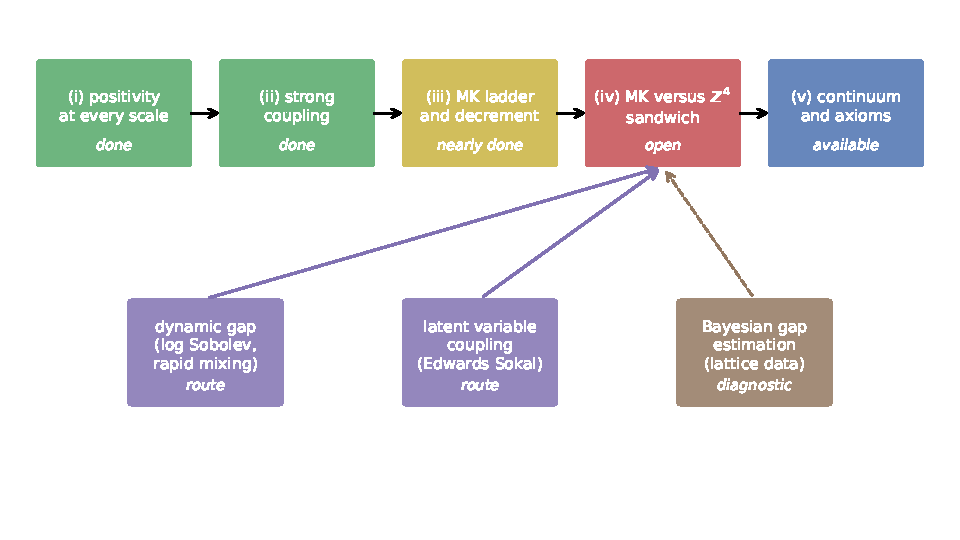
\includegraphics[width=\textwidth]{figures/roadmap.pdf}
\caption[A roadmap to the mass gap]{The five stages of the main path (top), colour coded by status, and three supporting routes (bottom): the dynamic gap through log Sobolev inequalities, a latent variable coupling in the style of Edwards and Sokal, and Bayesian gap estimation as a diagnostic.}
\label{fig:roadmap}
\end{figure}

The five stages of the path are those listed at the start of this chapter, and Figure~\ref{fig:roadmap} shows them with their status. Stage (iv), the comparison with $\Z^4$, is the step the next section is about.

\subsection{Three ways to attack stage (iv)}

\subsubsection*{A. A Thorin sandwich}
Bracket the true spectral measures directly. Its advantage is that the target statement is exactly the equivalence theorem; its weakness is that spectral measures are global objects and no local inequality is known to control them.

\subsubsection*{B. A dynamic sandwich}
Bracket Dirichlet forms of local dynamics along the ladder, and use the Stroock and Zegarlinski and Martinelli and Olivieri equivalences~\cite{SZ92,MO94} to convert a uniform log Sobolev inequality into a mass gap, which those equivalences give for finite range spin systems and which would have to be shown for gauge theory. Its advantage is that comparisons of Dirichlet forms are local and composable, and that the strong coupling end is already done by Shen, Zhu and Zhu~\cite{SZZ}. Its weakness is that log Sobolev constants are not known to behave monotonically under block spin transformations at weak coupling.

\subsubsection*{C. A latent variable coupling}
Realise the true block step and the Migdal Kadanoff step on one probability space, in the manner of Edwards and Sokal~\cite{ES88}, with latent variables chosen so that the plaquette laws are compared in the likelihood ratio order. Its advantage is that likelihood ratio orders are preserved by the two operations of the ladder when the kernels are log concave. Its weakness is that the Haar curvature breaks log concavity away from the identity; the Riemannian Pr\'ekopa Leindler inequality and Bakry \'Emery curvature on the three sphere are the tools one would try for it, although neither is known to give what is needed.

Our own preference is to try C first, then B, because they are local and because the probabilistic toolkit of this book is built for them. A is the cleanest statement and the hardest to attack directly.

\subsection{What would count as progress}

A complete proof is not the only useful outcome. In rough order of difficulty:
\begin{enumerate}
\item A rigorous, computer assisted version of stage (iii), giving an explicit gap function on hierarchical lattices for SU(2) and SU(3).
\item A comparison theorem in three dimensions, where the coupling is relevant rather than marginal and the stakes are lower.
\item A comparison theorem in four dimensions for a modified lattice action designed to make the comparison easier, for example with heat kernel plaquettes and a block spin rule adapted to Migdal Kadanoff.
\item A test of the Migdal Kadanoff predictions against published lattice glueball masses at intermediate coupling, by the estimator of Chapter~\ref{ch:estimation}.
\item The full comparison for the Wilson action.
\end{enumerate}

\subsection{Honest odds}

The mass gap has resisted fifty years of effort by people who knew more physics than we do. The approaches that came closest, Ba\l aban's renormalization group and Tomboulis's Migdal Kadanoff bracketing, both aim at the crossover between weak and strong coupling; the first stopped there and the second is not accepted as a proof. Our contribution is to put that crossover into a language, positive measures, Thorin densities, likelihood ratio orders, products and convolutions of laws on a curved group, in which probabilists have powerful tools, and to show by an exact result in two dimensions and by ladder computations that the language captures the mechanism. Whether the tools are strong enough for stage (iv) is unknown. We think the attempt is worth making, and the book is written so that others can make it.

\section{What We Might Be Missing}\label{ch:missing}\index{centre vortices}\index{gradient flow}\index{resurgence}\index{holography}

A book that proposes a route to an open problem should say which roads it has not taken. This section lists ideas from the physics and mathematics of gauge theory that we have not used, and for each says how it might bear on the approach of this book. It begins with recent work of others.

\subsection{Recent work of others}

Several recent results on lattice and continuum Yang Mills are close to our subject, though none is a mass gap for four dimensional Yang Mills at all couplings. On the lattice, Adhikari and Cao proved correlation decay for finite gauge groups at weak coupling~\cite{AC}; Cao, Park and Sheffield gave a random surface representation of lattice Yang Mills~\cite{CPS25}; and Cao, Nissim and Sheffield enlarged the regimes in which an area law is known, and gave a dynamical approach to it~\cite{CNS25}. In the continuum, the Yang Mills heat flow with random initial data~\cite{CC23} and stochastic quantisation have made progress in low dimensions: the Langevin dynamic of two dimensional Yang Mills~\cite{CCHS,ChSh23,BC23}, the local in time Langevin dynamic of three dimensional Yang Mills Higgs~\cite{CCHS3}, and, in two dimensions, the abelian Higgs equations~\cite{BC24} and the non abelian Yang Mills Higgs measure~\cite{BCHZ}. Chatterjee's survey~\cite{Ch19} is the place to start. These results concern finite groups at weak coupling, strong coupling, exact representations, lower dimensions, or a Higgs field, and the Thorin comparison of stage (iv) is not among them. The 2026 announcement of an existence proof for four dimensional Yang Mills~\cite{OAI,Woit26} is described in Section~\ref{sec:existence2026}.

\subsection{Centre vortices and 't Hooft's order parameters}

't Hooft~\cite{tH78} introduced the vortex free energy and the classification of phases of gauge theories by the behaviour of Wilson and 't Hooft loops. Mack and Petkova~\cite{MP80} gave a sufficient condition for confinement in terms of the free energy of a centre vortex, and Tomboulis's attempted proof~\cite{To07} used exactly this quantity, bracketing the twisted partition function between Migdal Kadanoff type bounds. Centre vortices are natural latent variables for the gauge field, and a latent representation built on them might supply the monotone coupling that Section~\ref{ch:isthere} asks for. We have not pursued this.

\subsection{Monopoles and dual superconductivity}

In three dimensional compact U(1), confinement is caused by monopoles, and G\"opfert and Mack~\cite{GM82} turned that into a theorem. In supersymmetric gauge theories Seiberg and Witten~\cite{SW94} showed that confinement follows from monopole condensation, the dual superconductor picture of Mandelstam~\cite{Ma76} and 't Hooft. No such mechanism has been established for pure nonabelian Yang Mills, but abelian projection and monopole condensation are widely studied on the lattice. A Thorin version of the G\"opfert and Mack argument, with the Coulomb gas of monopoles as the latent variables, is a direction we have not explored.

\subsection{Gradient flow}

L\"uscher's Yang Mills gradient flow~\cite{Lu10} smooths gauge fields along the gradient of the action. Observables at positive flow time are finite without renormalization, and the flow defines a scale. Flowed observables are the natural regularised operators for the offset measures of Chapter~\ref{ch:positivity}, and the flow itself is a deterministic renormalization map, close in spirit to the heat kernel convolution of the Migdal Kadanoff ladder. A comparison between the gradient flow and the ladder would make stage (iv) more concrete.

\subsection{Resurgence and renormalons}

The perturbative series of Yang Mills is not Borel summable, because of renormalons; Section~\ref{ch:sokal} discusses Borel summability. The theory of resurgence aims to reconstruct nonperturbative quantities from the large order behaviour of perturbation theory together with semiclassical saddles. The mass gap, of order $\Lambda$, is exactly such a quantity. We have not tried to connect resurgence with the Thorin structure, although Borel transforms and Laplace transforms of positive measures are close relatives.

\subsection{Holography}

The gauge gravity correspondence gives models of confining theories whose glueball spectra are computed from normal modes of fields in a curved higher dimensional geometry, as Witten and others showed in 1998~\cite{Wi98}. The spectral problem there is a Sturm Liouville problem, whose spectral measures are discrete and positive, and the gap is the lowest eigenvalue of a differential operator. These models are not pure Yang Mills, but they are caricatures in Kac's sense in which the gap is computable.

\subsection{Hamiltonian lattice gauge theory and quantum computation}

Kogut and Susskind's Hamiltonian formulation~\cite{KS75} puts the gauge theory on a spatial lattice with continuous time. The gap is then the gap of an explicit operator on a Hilbert space spanned by spin networks, the representation labels of Section~\ref{ch:latent}. Tensor network methods and quantum simulation target this formulation directly. The positivity of the transfer matrix is replaced by the self adjointness of the Hamiltonian, and the question becomes a spectral gap problem for a quantum many body system, where techniques such as the detectability lemma and martingale methods for frustration free Hamiltonians exist.

\subsection{Formal verification}

The existence proof announced in 2026 comes with a Lean formalisation~\cite{OAI}. Any proof of the mass gap will be long, multiscale, and partly computer assisted, and its credibility will depend on formal verification. Stage (iii) of the path, a computer assisted version of the gap statement on hierarchical lattices, is a natural first target for formalisation once its conditions are proved: it involves explicit special functions, interval arithmetic, and a monotone covering argument.

\subsection{Things we missed and have since found}

Some of what later chapters contain belongs under this title. We record five items here, because each changed our view of the problem, and at least one of them corrects a mistake.

\subsubsection*{Classical loop inequalities}
We listed $W_{12}\ge W_{11}^2$ as an open problem for nonabelian groups and tested it by simulation at eleven couplings. It is a three line consequence of reflection positivity for every compact group (Theorem~\ref{thm:doubling}). The lesson is general: reflection positivity gives a positive inner product, and every Schwarz inequality in it is a theorem about Wilson loops. The literature of the late 1970s and 1980s contains many, among them the convexity of the static potential and upper bounds on the string tension. Before posing a comparison as a conjecture one should ask whether it is a Schwarz or chessboard inequality.

\subsubsection*{The abelian control}
Any argument for confinement at weak coupling must fail for compact U(1) in four dimensions, where Guth~\cite{Gu80}, and Fr\"ohlich and Spencer~\cite{FS82}, proved that there is a massless Coulomb phase. This is the sharpest test of a proposed mechanism, and we had not applied it to the ladder. Doing so is instructive (Figure~\ref{fig:u1ladder}). On U(1) the heat kernel is a wrapped Gaussian, the group is flat, and bond moving maps the family to itself up to the images: the decrement of the ladder is not $\frac14$ but exponentially small, about $2\times10^{-5}$ at $\beta=1$, $4\times10^{-11}$ at $\beta=2$ and $2\times10^{-23}$ at $\beta=4$. So the ladder separates abelian from nonabelian theories by the mechanism this book has emphasised: no curvature, no running. But it does not produce a Coulomb phase. The decrement is positive, the flow still reaches strong coupling after a number of steps that grows exponentially in $\beta$, and the ladder predicts confinement with an astronomically large correlation length, which is false. The Migdal Kadanoff recursion is known to behave this way at a lower critical dimension. For the comparison problem the consequence is concrete: for U(1) the lower bracket must be a map with a line of fixed points, so no pair of brackets that both have positive decrement can be valid for all compact groups. A proof of the sandwich must use nonabelian structure, and the product formula and the curvature terms of Theorem~\ref{thm:expansionN} are where it enters.

\begin{figure}[t]
\centering
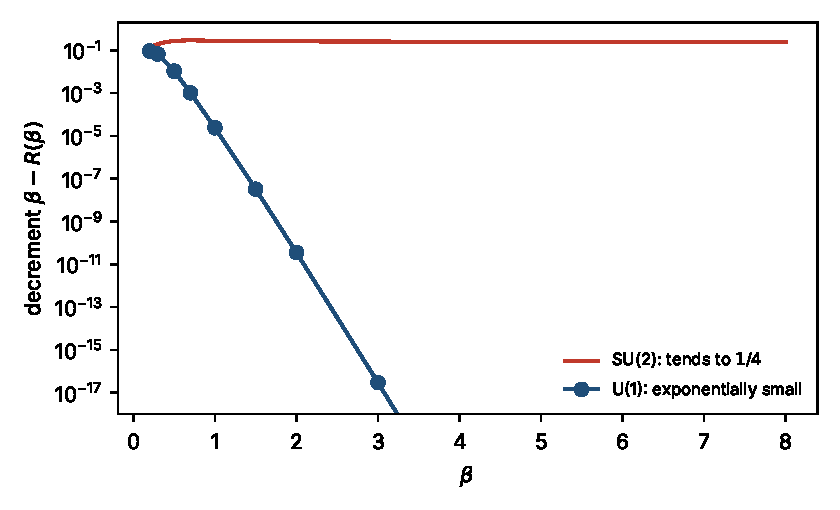
\includegraphics[width=0.8\textwidth]{figures/u1_ladder.pdf}
\caption[The abelian control: the ladder for U(1) and SU(2)]{The decrement $\beta-R(\beta)$ of the Migdal Kadanoff ladder in four dimensions with $b=2$, for SU(2), where it tends to $\frac14$, and for compact U(1) with heat kernel laws, where it is exponentially small in $\beta$.}
\label{fig:u1ladder}
\end{figure}

\subsubsection*{The centre, the antipode and the crossover}
Three known phenomena sit in the window of couplings where our methods are weakest, and we had not connected them. The first is the phase structure in the plane of fundamental and adjoint couplings found by Bhanot and Creutz~\cite{BC81}: an action with an adjoint term has first order transitions, driven by the centre element $-1$ and its $\Z_2$ monopoles, on lines that end at a critical point close to the Wilson axis. The rapid crossover of the Wilson theory near $\beta=2.2$, and the failure of asymptotic scaling there, are usually attributed to that nearby endpoint. The second is the roughening transition of the strong coupling expansion near $\beta=1.9$, beyond which the series for the string tension cannot be continued. The third is our own bad cap at the antipode (Theorem~\ref{thm:hemisphere}), which is the same centre element seen in the convolution kernel, and whose mass peaks at $\beta\approx0.8$ in the ladder's coordinate, roughly $\beta\approx2.2$ after the shift of $1.45$ found in Chapter~\ref{ch:progress}. The ladder acts on whole plaquette laws, so it has an adjoint coupling, the coefficient $u_3$; following the flow in the plane $(u_2,u_3)$ against the Bhanot and Creutz diagram, and repeating the tests of Chapter~\ref{ch:progress} for the heat kernel and positive plaquette actions, which were designed to remove the centre artefacts, is a computation we have not done.

\subsubsection*{Finite temperature and our small lattices}
A periodic lattice of temporal extent $N_t$ is a system at temperature $1/(N_ta)$, and SU(2) deconfines above a critical coupling: $\beta_c=2.30$ for $N_t=4$ and $2.51$ for $N_t=8$~\cite{FHK}. Our $8^4$ runs at $\beta\ge3$ and all our $4^4$ runs above $\beta=2.3$ are therefore in small, hot boxes, not in the confined phase of the infinite lattice. For the quantities we measured this is harmless and in one case intended: plaquettes and $2\times2$ loops are local, their finite size corrections are small, and the agreement with the perturbative values tabulated for Conjecture~\ref{prop:weaksandwich}, computed on the same $8^4$ lattice, confirms it; the matching of Section~\ref{ch:plgbc} compares two lattices of the same physical size by design. But no string tension or glueball mass could be extracted from those runs, and the text should not be read as if it could. The deconfinement transition is also a subject we have left out: the Polyakov loop, centre symmetry and the Svetitsky and Yaffe universality argument~\cite{SY82} give a second, well understood order parameter for confinement.

\subsubsection*{The Hamiltonian form}
Proposition~\ref{prop:groundstate} of Section~\ref{ch:h6ym} states the gap in terms of the Poincar\'e constant of the ground state measure. We had treated the Hamiltonian formulation only as a topic for quantum simulation. It deserves more: it is the form of the problem in which the gap is the spectral gap of a single diffusion.

\subsection{Loop equations and the bootstrap}

The Schwinger Dyson equations of lattice gauge theory, the Makeenko and Migdal loop equations~\cite{MM79}, relate the expectation of a Wilson loop to those of loops deformed by one plaquette. In the dictionary of Section~\ref{ch:dictionary} they are score equations. Chatterjee~\cite{Ch19so}, and Shen, Smith and Zhu, have derived and used them rigorously. In the last few years they have been combined with positivity into a numerical bootstrap: Anderson and Kruczenski~\cite{AK17}, and Kazakov and Zheng~\cite{KZ23}, impose the loop equations as linear constraints on a finite set of loop expectations and reflection positivity as the semidefiniteness of matrices of such expectations, and obtain rigorous two sided bounds on the plaquette that tighten as the set grows.

This is close to the present book and we have not used it. The semidefinite matrices of the bootstrap are the Hankel and Gram matrices of Chapter~\ref{ch:positivity}; Theorem~\ref{thm:doubling} is one of their two by two minors. The bootstrap is a systematic way to generate comparison inequalities of exactly the kind the sandwich needs, with a certificate. Two uses suggest themselves. A bootstrap bound on $W_{22}$ given $W_{11}$ would be a rigorous bracket to set beside the two caricatures. And a bootstrap on correlators at several time separations, with the gap as the variable, is the certified version of the estimator of Chapter~\ref{ch:estimation}: the largest $m$ for which a positive spectral measure supported on $[m,\infty)$ is consistent with the loop equations.

\subsection{Generalised symmetries}

Since the work of Gaiotto, Kapustin, Seiberg and Willett~\cite{GKSW}, confinement in pure gauge theory is described as the statement that a one form symmetry, the centre symmetry acting on Wilson loops, is unbroken: the area law is the disordered phase of that symmetry and the perimeter law its broken phase. Anomaly matching for this symmetry constrains the possible long distance behaviour, for instance at vacuum angle $\pi$. This language gives precise meaning to the order parameters of 't Hooft, organises the role of the centre that appears in several places above, and suggests that the right object for a comparison theorem is not the plaquette law alone but the pair consisting of the Wilson loop and the centre vortex free energy, which are dual under the symmetry. Tomboulis's attempted proof~\cite{To07} worked with that pair.

\subsection{Gauge fixed and functional methods}

A large physics literature approaches the gap through gauge fixed correlation functions: Gribov's restriction of the functional integral~\cite{Gr78}, Zwanziger's horizon condition, Cornwall's dynamically generated gluon mass, and functional renormalization group and Dyson Schwinger studies of the Landau gauge propagators, checked against lattice simulations in fixed gauges. These methods produce a mass scale in the gluon propagator. They are not rigorous, they work with quantities that are not gauge invariant and not reflection positive, and their relation to the gauge invariant spectral measures of this book is indirect. But they are the main source of quantitative intuition about how a mass arises at intermediate momenta, and a probabilistic reading of the Gribov region, as a constraint set of the kind met in slice sampling, may be worth having.

\subsection{Statistics we have not used}

Finally, two statistical ideas we have not developed. Empirical Bayes estimation of the spectral measure across many lattice spacings, borrowing strength along the renormalized trajectory, would sharpen the gap estimator of Chapter~\ref{ch:estimation}. And generative Bayesian computation, which learns a map from data to posterior through deep networks, could learn the renormalization map itself from simulations, giving an empirical version of the ladder against which the Migdal Kadanoff caricature could be compared.

\section{Three Dimensions First}\label{ch:threed}\index{three dimensions}\index{Karabali, D.!Kim, C. and Nair, V. P.}\index{Teper, M.}

The tests of Chapter~\ref{ch:progress} recommend three dimensions as the place to attempt the comparison step. This section says why, collects what is known there, and states the three dimensional version of the path.

\subsection{Why three dimensions is easier}

In three dimensions the gauge coupling $g^2$ has the dimension of mass. The theory is superrenormalizable: there is no logarithmic running, the coupling is relevant, and the lattice coupling $\beta=4/(ag^2)$ for SU(2) is simply proportional to the inverse lattice spacing. All masses are multiples of $g^2$, and the continuum limit is $\beta\to\infty$ with $a=4/(\beta g^2)$.

For the ladder this changes everything that was delicate in four dimensions. The Gaussian ledger of Section~\ref{ch:mk} gives, per step of scale factor $b$,
\[
\frac1{t''}=\frac{b^{-1}}{t}-\frac{(b-1)\,\E S_{\mathrm{BPY}}}{2b^2}+O(t),
\]
so the inverse coupling $1/t$ is divided by $b$ at every step whatever the curvature term does, and the number of steps to strong coupling is $\log_b\beta$ up to a constant. The scale is set by counting, not by an exponentially sensitive crossover. An error in the curvature term changes the answer by a factor near one, not by a factor of fifty.

\subsection{What is known}

Ultraviolet stability in three dimensions is part of Ba\l aban's programme and is simpler than in four. The mass gap is open in three dimensions too: no proof of confinement or of a gap exists for the nonabelian theory at weak lattice coupling. For compact U(1) in three dimensions, G\"opfert and Mack~\cite{GM82} proved confinement and a mass gap at all couplings, by the monopole gas. Numerically the theory is known to high precision: Teper's simulations~\cite{Te99} give $\sqrt\sigma/g^2=0.3353$ for SU(2), with glueball masses in fixed ratio to $\sqrt\sigma$.

There is also an analytic prediction. Karabali, Kim and Nair~\cite{KKN}, working in the Hamiltonian formulation with gauge invariant matrix variables, obtained
\[
\sqrt\sigma=g^2\sqrt{\frac{N^2-1}{8\pi}},
\]
which is $0.3455\,g^2$ for SU(2), three percent above the lattice value. Their vacuum wave functional is, to leading order, Gaussian in the magnetic field with a kernel that has a gap, and the string tension is that of a two dimensional Yang Mills theory with an effective coupling. In the language of this book: the three dimensional vacuum, restricted to a plane, looks like a two dimensional heat kernel measure, the exactly solvable case of Chapter~\ref{ch:twod}.

\subsection{The ladder in three dimensions}

\begin{figure}[t]
\centering
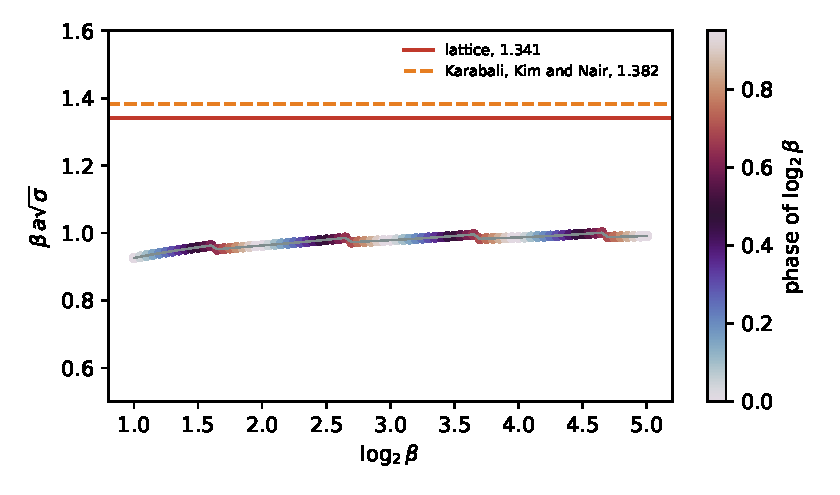
\includegraphics[width=0.9\textwidth]{figures/mk_3d.pdf}
\caption[The three dimensional ladder against lattice and analytic values]{The ladder's prediction of $\beta a\sqrt\sigma$ for three dimensional SU(2) as a function of $\log_2\beta$, coloured by the phase of $\log_2\beta$, against the lattice continuum value and the prediction of Karabali, Kim and Nair. The ladder is flat in $\log_2\beta$ at weak coupling to within two percent; the small remaining modulation is an artefact of the discrete scale factor.}
\label{fig:mk3d}
\end{figure}

With no fitted constant, the ladder with $b=2$ and Wilson start gives $\beta a\sqrt\sigma$ between $0.98$ and $1.00$ for $8\le\beta\le32$, with mean $0.99$ over a period of $\log_2\beta$ (Figure~\ref{fig:mk3d}; computed by \texttt{code/mk\_sigma.py}, run from \texttt{code/mk\_3d.py}). The lattice value is $1.341$ and the analytic prediction $1.382$. The ladder is low by twenty six percent on average. The remaining modulation, about two percent peak to peak, is an artefact of the discrete scale factor: the true theory has no preferred scale factor, and the modulation measures how much the answer depends on where the integer number of steps happens to end.

Twenty six percent is the size of bracket that a comparison theorem in three dimensions must tolerate. Since the conclusion sought is only that the string tension and the gap are positive multiples of $g^2$, and not their values, a bracket of that width is harmless.

\subsection{The sandwich in three dimensions}

Chapter~\ref{ch:sandwich} measured the laws of the $2\times2$ and $4\times4$ loops on a $16^3$ lattice. We collect the three dimensional numbers here, since they are the evidence for the problem below.

\begin{center}
\small
\begin{tabular}{ccccccc}
\toprule
 & \multicolumn{3}{c}{$u_2$ of the $2\times2$ loop} & \multicolumn{3}{c}{$u_2$ of the $4\times4$ loop} \\
$\beta$ & indep. & measured & MK & indep. & measured & MK \\ \midrule
4 & 0.281 & 0.323 & 0.540 & 0.0062 & 0.021 & 0.267 \\
6 & 0.463 & 0.522 & 0.686 & 0.046 & 0.126 & 0.456 \\
9 & 0.615 & 0.672 & 0.787 & 0.143 & 0.305 & 0.613 \\
14 & 0.739 & 0.785 & 0.862 & 0.298 & 0.494 & 0.740 \\
\bottomrule
\end{tabular}
\end{center}

At one step the two caricatures differ by a factor between $1.2$ and $1.9$, and the truth sits about a third of the way from the independent end. At two steps they differ by a factor between $2.5$ and $43$, and the truth is near the middle on a logarithmic scale. At weak coupling perturbation theory gives $\log W_{22}/\log W_{11}=3.120$ and $\log W_{44}/\log W_{11}=8.715$, against $4$ and $16$ for independent plaquettes and $2$ and $4$ for the ladder; the measured ratio at $\beta=14$ is $3.21$.

\subsection{The path in three dimensions}

\begin{enumerate}
\item[1.] Positivity. Reflection positivity on the lattice and the preservation of nonnegative character coefficients by the ladder hold in any dimension; reflection positivity for a block spin transformation of the true flow is not shown, as in four dimensions.
\item[2.] Strong coupling. The cluster expansion and the log Sobolev argument are not specific to four dimensions.
\item[3.] The ladder. In three dimensions the map $\beta\mapsto R_3(\beta)$ contracts at weak coupling by the factor $b$. The decrement inequality $R_3(\beta)<\beta$ is immediate there, and the covering argument is needed only on a bounded range near the crossover. Monotonicity is Corollary~\ref{cor:mlrall}, which does not depend on the dimension.
\item[4.] The comparison. The empirical sandwich of Chapter~\ref{ch:sandwich} holds in three dimensions at every coupling and scale we tried; there bond moving has power $b$ and not $b^2$, and the two caricatures are closer together. Because the flow is contracting, errors in a single step do not accumulate multiplicatively in the scale as they do when the coupling is marginal.
\item[5.] The continuum. Superrenormalizability makes the ultraviolet limit far simpler than in four dimensions.
\end{enumerate}

\begin{problem}\label{op:path7}
Prove that three dimensional SU(2) lattice gauge theory with the Wilson action has a mass gap $m(\beta)\ge c_0/\beta$ in lattice units for all $\beta$, with $c_0>0$, by bracketing one block spin step between two contracting Migdal Kadanoff type maps.
\end{problem}

This is the problem we would work on first. It is open, it is believed true, the exactly solvable two dimensional theory sits inside it through the Karabali, Kim and Nair picture, and every tool of this book applies without the marginal flow that makes four dimensions hard.

\section*{Exercises}
\begin{enumerate}
\item Derive the three dimensional ledger of Section~\ref{ch:threed} from the general formula of Section~\ref{ch:mk} and show that the number of steps to strong coupling is $\log_b\beta+O(1)$.
\item Show that a function of the form $\beta a\sqrt\sigma$ computed from a recursion with scale factor $b$ is asymptotically periodic in $\log_b\beta$ at weak coupling.
\item Compute the Karabali, Kim and Nair value of Section~\ref{ch:threed} for SU(3) and compare it with the lattice value $0.5530$.
\end{enumerate}

\chapter{Progress on the Open Problems}\label{ch:progress}\index{product formula}\index{Laguerre P\'olya class}\index{likelihood ratio order}\index{effective coupling}\index{Parisi, G.}\index{string tension}\index{scale factor}

This chapter reports our own progress, made in this book, on the open problems listed in Chapter~\ref{ch:path}. It is not a survey of the literature: the recent work of others on lattice Yang Mills is discussed in Section~\ref{ch:missing}, and the history in Chapter~\ref{ch:programme}. The SU(2) half of the second problem is closed: the likelihood ratio property of the SU(2) heat kernel, on which the monotonicity of the projected ladder rests, is now a theorem at every time, by a product formula for the heat kernel. The chapter also proves the weak coupling expansion of the ladder (Theorems~\ref{thm:expansion} and~\ref{thm:expansionN}), total positivity of convolution (Theorem~\ref{thm:tp2}), and that the ladder contracts (Theorem~\ref{thm:scaledmlr} and Corollary~\ref{cor:contracts}); the rest are quantitative tests of the ladder against lattice data. They give an honest mixed verdict: the ladder predicts the rate of running to within ten or fifteen percent, has about half the correct two loop coefficient, and misplaces the crossover to strong coupling.

\section{A product formula for the heat kernel}

Write the SU(2) heat kernel in the normalisation of Section~\ref{ch:verification},
\[
K_t(\theta)=\sum_{n\ge1}n\,e^{-(n^2-1)t/4}\,\frac{\sin n\theta}{\sin\theta},
\]
and put $c=\cos\theta$ and $C_n(t)=\cosh\big((2n-1)t/4\big)$.

\begin{theorem}[product formula]\label{thm:product}
For every $t>0$,
\[
K_t(\theta)=K_t(\pi/2)\prod_{m\ge1}\Big(1+\frac{\cos\theta}{\gamma_m(t)}\Big),
\]
where $\gamma_1<\gamma_2<\cdots$ are the roots of
\[
\sum_{n\ge1}\frac{1}{C_n(t)-\gamma}=0,\qquad C_m(t)<\gamma_m(t)<C_{m+1}(t).
\]
In particular every $\gamma_m(t)$ exceeds one. Each $\gamma_m$ is strictly increasing in $t$, with
\[
\gamma_m'(t)=\sum_{n\ge1}w_{mn}\,C_n'(t),\qquad w_{mn}=\frac{(C_n-\gamma_m)^{-2}}{\sum_{l}(C_l-\gamma_m)^{-2}} .
\]
\end{theorem}

\begin{proof}
Let $\nu=e^{-t/4}$ and $\vartheta(\theta)=\sum_{n\in\Z}\nu^{n^2}e^{in\theta}$, the heat kernel of the circle. Since $-\partial_\theta\vartheta=2\sum_{n\ge1}n\nu^{n^2}\sin n\theta$ and $\partial_\theta=-\sin\theta\,\partial_c$,
\[
K_t(\theta)=\frac{e^{t/4}}{2}\,\frac{\mathrm d\vartheta}{\mathrm dc}.
\]
The Jacobi triple product gives $\vartheta=\prod_{n\ge1}(1-\nu^{2n})\cdot P(c)$ with
\[
P(c)=\prod_{n\ge1}\big(1+\nu_n^2+2\nu_nc\big),\qquad \nu_n=\nu^{2n-1}.
\]
As a function of $c$, $P$ is entire of order zero, with simple real zeros at $c=-(1+\nu_n^2)/(2\nu_n)=-C_n(t)$. By Laguerre's theorem~\cite{PS14} the derivative of such a function has only real simple zeros, one in each gap between consecutive zeros of $P$, and is again of order zero. Hadamard's factorisation therefore has no exponential factor, and $P'(c)=P'(0)\prod_m(1+c/\gamma_m)$ with $-\gamma_m\in(-C_{m+1},-C_m)$. The equation for the roots is $P'/P=\sum_n(c+C_n)^{-1}=0$ at $c=-\gamma$.

For the motion of the roots, differentiate $\sum_n(C_n(t)-\gamma_m(t))^{-1}=0$ in $t$; the series converges locally uniformly with its derivative, because $C_n$ grows like $e^{nt/2}$. This gives $\sum_n(C_n'-\gamma_m')(C_n-\gamma_m)^{-2}=0$, which is the stated formula. The weights $w_{mn}$ are positive and sum to one, and $C_n'(t)=\frac{2n-1}{4}\sinh((2n-1)t/4)>0$.
\end{proof}

The proof is the classical fact that the critical points of a function with real zeros move as convex combinations of the velocities of the zeros. Here every zero $-C_n(t)$ moves to the left as $t$ grows, so every critical point does too.

\begin{corollary}[likelihood ratio property]\label{cor:mlrall}
For every $t>0$ and $\theta\in(0,\pi)$,
\[
\partial_t\,\partial_\theta\log K_t(\theta)=\sin\theta\sum_{m\ge1}\frac{\gamma_m'(t)}{(\gamma_m(t)+\cos\theta)^2}>0 .
\]
The SU(2) heat kernel has strictly monotone likelihood ratio in time, the hypothesis of Lemma~\ref{lem:mlrB} holds, and the projected Migdal Kadanoff map $R$ is increasing at every coupling and for every scale factor $b$.
\end{corollary}

\begin{corollary}[log concavity]\label{cor:logconc}
For every $t>0$ the heat kernel is strictly log concave as a function of $c=\cos\theta$ on $[-1,1]$, with $\partial_c^2\log K_t=-\sum_m(\gamma_m+c)^{-2}$. The same holds for every power $K_t^k$, hence for every plaquette law produced by bond moving from a heat kernel law.
\end{corollary}

\begin{corollary}[Thorin form]\label{cor:thorinform}
For every $t>0$, with $x=\cos\theta$,
\[
\frac{K_t(\pi/2)}{K_t(\theta)}=\prod_{m\ge1}\frac{\gamma_m(t)}{\gamma_m(t)+x}=\E\,e^{-xT_t},\qquad T_t=\sum_{m\ge1}\frac{E_m}{\gamma_m(t)},
\]
with independent standard exponential $E_m$. So the reciprocal of the heat kernel, as a function of $x=\cos\theta$, is the Laplace transform of a generalized gamma convolution whose Thorin measure $\sum_m\delta_{\gamma_m(t)}$ has integer masses and is supported on $(1,\infty)$, beyond the edge of the group, with atoms moving to the right as $t$ grows.
\end{corollary}
\begin{proof}
By Theorem~\ref{thm:product}, $K_t=K_t(\pi/2)\prod_m(1+x/\gamma_m(t))$ with every $\gamma_m(t)>1$, increasing in $t$, and $\sum_m1/\gamma_m(t)<\infty$ because $\gamma_m(t)>C_m(t)$; so $K_t$ is in the class $\mathcal L$ of Chapter~\ref{ch:zeros}, and $\E\,e^{-xE_m/\gamma_m}=\gamma_m/(\gamma_m+x)$ for $x>-\gamma_m$.
\end{proof}

Three remarks. First, as a function of $c$ the heat kernel belongs to the Laguerre P\'olya class~\cite{PS14}: it is a limit of polynomials with only real zeros, all outside the interval $[-1,1]$ on which it is a density. This is the P\'olya class~\cite{Po26}, in which the Riemann $\Xi$ function~\cite{Ri59} lies exactly when the Riemann Hypothesis holds, and the argument above is of de Bruijn Newman type~\cite{dB50,Ne76}: under the heat flow the zeros move monotonically, here away from the support. Section~\ref{ch:rhbooks} (Chapter~\ref{ch:kacyang}) returns to this. Second, the product formula gives a sampler: $K_t$ is a product of linear factors in $c$, so it can be bounded above by its first factors for rejection sampling at any $t$. Third, the corollaries are strict for every $t>0$ and every $\theta\in(0,\pi)$.

\begin{figure}[t]
\centering
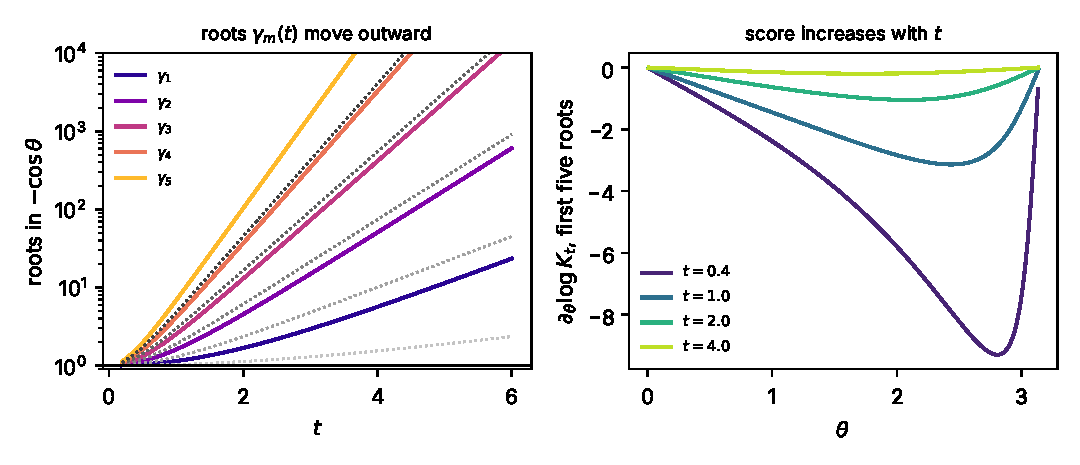
\includegraphics[width=\textwidth]{figures/heat_roots.pdf}
\caption[Roots of the SU(2) heat kernel]{Left: the first five roots $\gamma_m(t)$ of the heat kernel in the variable $-\cos\theta$, solid, interlaced with the zeros $C_n(t)=\cosh((2n-1)t/4)$ of the theta function, dotted. All move outward as $t$ grows. Right: the score $\partial_\theta\log K_t$ computed from the first five roots; it increases with $t$ at every angle.}
\label{fig:heatroots}
\end{figure}

We checked the product formula numerically: with forty roots, computed in forty digit arithmetic, the ratio of the character series to the product is constant in $\theta$ to $10^{-8}$ at $t=1$, $10^{-17}$ at $t=2$ and $10^{-31}$ at $t=4$, and every computed root increases with $t$ (Figure~\ref{fig:heatroots}). Figure~\ref{fig:mlrratios} shows the property directly, and Figure~\ref{fig:mlrheat} maps the mixed partial over the whole time range, computed independently from the Poisson resummed image sum; its normalised minimum on $[0.04,3.41]$ is $0.67$.

\begin{figure}[t]
\centering
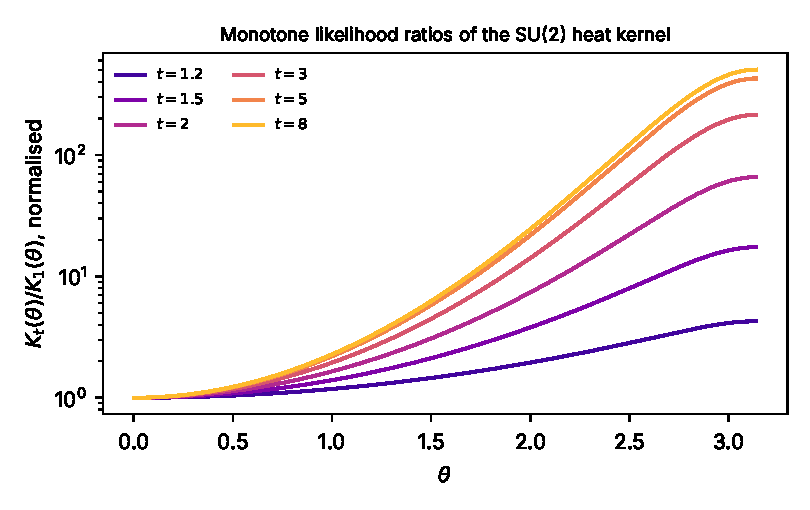
\includegraphics[width=0.85\textwidth]{figures/mlr_ratios.pdf}
\caption[Likelihood ratios of the SU(2) heat kernel]{Likelihood ratios $K_t(\theta)/K_1(\theta)$ of the SU(2) heat kernel, normalised at $\theta=0$, for six times. Each is increasing in $\theta$, which is the monotone likelihood ratio property.}
\label{fig:mlrratios}
\end{figure}

\begin{figure}[t]
\centering
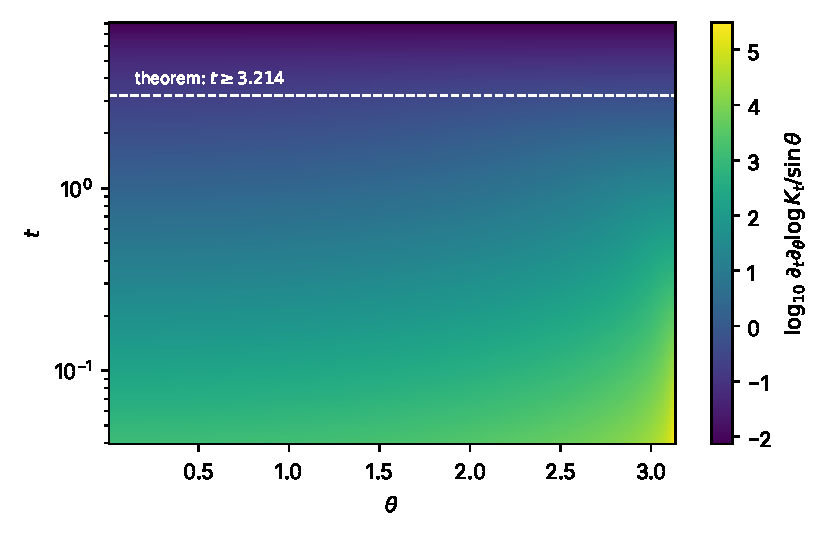
\includegraphics[width=0.9\textwidth]{figures/mlr_heatmap.pdf}
\caption[The mixed partial of the log heat kernel]{The normalised mixed partial $\partial_t\partial_\theta\log K_t(\theta)/\sin\theta$ on a logarithmic colour scale, computed from the image sum. It is positive everywhere, as Corollary~\ref{cor:mlrall} requires. The dashed line marks $t=3.214$, above which the elementary bound of Proposition~\ref{thm:mlrlarge} also applies.}
\label{fig:mlrheat}
\end{figure}

\section{Two other proofs, and the Wilson law}

Before finding the product formula we had two partial arguments. Both are worth recording because they generalise in different directions.

\begin{proposition}[elementary bound at large time]\label{thm:mlrlarge}
With $\varepsilon_n(t)=n\,e^{-(n^2-1)t/4}$, let
\begin{align*}
\Phi(t)={}&6\varepsilon_2-\sum_{n\ge3}\frac{(n^2-1)(n^3-n)}{3}\,\varepsilon_n\\
&-\frac{\big(\sum_{n\ge2}(n^2-1)n\,\varepsilon_n\big)\big(\sum_{m\ge2}\frac{m^3-m}{3}\varepsilon_m\big)}{1-\sum_{n\ge2}n\,\varepsilon_n}.
\end{align*}
Then $4\,\partial_t\partial_\theta\log K_t(\theta)\ge \Phi(t)\sin\theta/K_t(\theta)$ whenever the denominator is positive, and $\Phi(t)>0$ for all $t\ge3.2140$.
\end{proposition}

\begin{proof}
Differentiate the character series term by term and use three bounds: $\partial_\theta U_1(\cos\theta)=-2\sin\theta$ for the leading term; the bound $|U_{n-1}'|\le U_{n-1}'(1)=(n^3-n)/3$ on $[-1,1]$ for the rest, which holds because $U_{n-1}'=2C^{(2)}_{n-2}$ is a Gegenbauer polynomial of positive index and so attains its largest modulus on $[-1,1]$ at $x=1$; and $|U_{n-1}|\le n$. The function $e^{3t/4}\Phi(t)$ is increasing with limit $12$, and a bisection in thirty digit arithmetic locates its zero at $3.2140$.
\end{proof}

The proof above uses the Chebyshev series of SU(2), so the proposition is stated for SU(2) only. The argument uses little beyond the gap of the Laplacian between its first two levels, so we expect it to extend to any compact group and to SU(3), where no product formula in one variable is available; we have not written the extension.

The second argument is a maximum principle. Let $\rho_t$ solve the radial heat equation $\partial_t\rho=\frac14(\rho''+2\cot\theta\,\rho')$ on $(0,\pi)$, and put $v=\partial_\theta\log\rho$ and $z=\partial_tv$. Then
\[
4\,\partial_tz=z''+(2v+2\cot\theta)\,z'+\Big(2v'-\frac{2}{\sin^2\theta}\Big)z ,
\]
a linear parabolic equation with $z=0$ at both ends by symmetry. If $z\ge0$ at one time it stays nonnegative, by the maximum principle (Section~\ref{ch:proofs2} of the appendix). For the heat kernel this reduces the property at all times to the property at arbitrarily small times. For other initial laws it gives new information.

\begin{proposition}[Wilson law]\label{prop:wilsonflow}
Let $\rho_0(\theta)\propto e^{\kappa\cos\theta}$ be the Wilson~\cite{Wi74} plaquette law and $\rho_t$ its heat flow. At $t=0$,
\[
4\,\partial_t\partial_\theta\log\rho_t=\kappa\sin\theta\,(3+2\kappa\cos\theta).
\]
Hence the family $(\rho_t)_{t\ge0}$ has monotone likelihood ratio in time if and only if $\kappa\le3/2$.
\end{proposition}

\begin{proof}
With $v=-\kappa\sin\theta$, compute $v''+2vv'+2\cot\theta\,v'-2v/\sin^2\theta=\kappa\sin\theta+2\kappa^2\sin\theta\cos\theta+2\kappa\sin\theta$. This is nonnegative on $(0,\pi)$ exactly when $\kappa\le3/2$, and the maximum principle propagates the sign. For $\kappa>3/2$ the property fails near $\theta=\pi$ at small times.
\end{proof}

A numerical check agrees: the minimum of the mixed partial over a grid of times and angles is positive for $\kappa=0.5$, $1$ and $1.5$ and negative for $\kappa=2$ and $3$. The threshold has a meaning. The Wilson law at $\kappa>3/2$ has too little mass near the antipode $-1$ relative to any heat kernel, and the flow first repairs that. This is a precise version of the statement that the Wilson action and the heat kernel action differ near the centre element, the region responsible for the lattice artefacts that the positive plaquette and heat kernel actions were designed to remove.

\section{A first look at SU(3)}

For SU(3) the heat kernel is a function on the maximal torus, of two angles, and there is no product formula in one variable. The natural analogue of the likelihood ratio property is along rays from the identity: for $\theta=r\mathbf e$ with $\mathbf e$ a direction in the Weyl alcove, is $\partial_t\partial_r\log K_t(r\mathbf e)\ge0$? We computed the heat kernel from its character expansion with all representations of Dynkin labels $p+q\le60$, on four rays and seventy times in $[0.12,6]$, out to $98$ percent of the distance at which the ray leaves the alcove (Figure~\ref{fig:su3mlr}).

\begin{figure}[t]
\centering
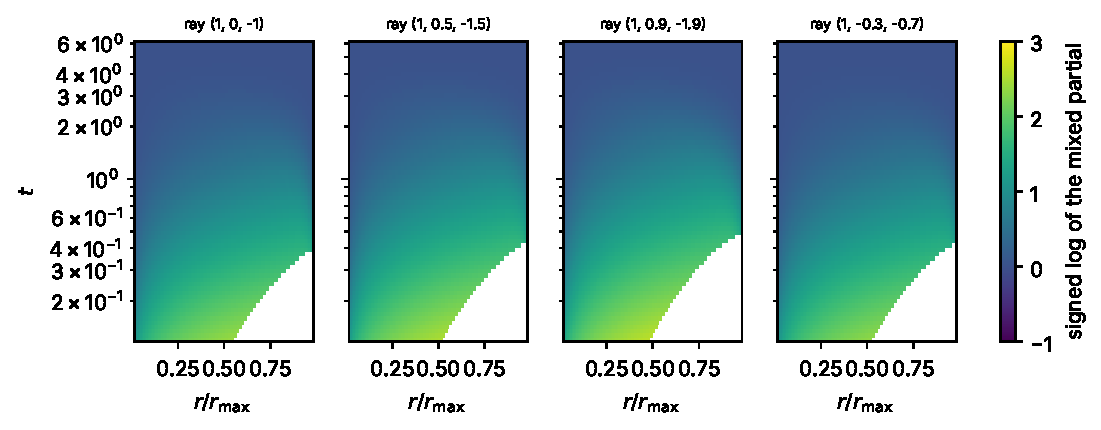
\includegraphics[width=\textwidth]{figures/su3_mlr.pdf}
\caption[The likelihood ratio property for SU(3) along rays]{The mixed partial $\partial_t\partial_r\log K_t(r\mathbf e)$ of the SU(3) heat kernel along four rays from the identity in the Weyl alcove, on a signed logarithmic colour scale. It is positive wherever the kernel exceeds $10^{-6}$; the blank corner at small time and large distance is where the character sum loses precision.}
\label{fig:su3mlr}
\end{figure}

On every ray the mixed partial is positive at every grid point where the kernel is larger than $10^{-6}$, about ninety percent of the grid; the excluded points lie at small time and large distance, where the kernel is smaller than the rounding error of the sum. The minimum over the grid is about $3\times10^{-4}$; at large time and small distance the mixed partial tends to zero, as it does for SU(2). So the property holds numerically for SU(3) along rays. A proof might come from the Gaussian sum over the coroot lattice, in which each image is log supermodular in $(t,r)$ and the Weyl denominator does not depend on $t$, or from a two variable form of the Laguerre argument.

\begin{quote}
\textsc{Status.} The likelihood ratio property of the SU(2) heat kernel is a theorem at every time. The projected ladder map is therefore monotone without numerical input, the contraction $R(\beta)<\beta$ is proved outright in Corollary~\ref{cor:contracts}, and the covering of Remark~\ref{prop:coverB} needs only interval arithmetic for the map itself to become a computer assisted proof. For SU(3) numerics give the property along rays; a proof, at large time or otherwise, is open.
\end{quote}

\section{A first test against lattice data}

The ladder predicts that the lattice spacing halves each time $\beta$ increases by the decrement, $1/4$ at weak coupling for SU(2) with $b=2$. Hence $d\log a/d\beta=-4\log2=-2.77$. Perturbation theory predicts the asymptotic value $-1/(4Nb_0)=-2.69$ at one loop and, with the two loop correction at $\beta=2.5$, a local slope of $-2.52$. We compare with the string tension of the Wilson action measured on large lattices, $a\sqrt\sigma=0.4690$, $0.3690$, $0.2660$, $0.1871$ and $0.1207$ at $\beta=2.2$, $2.3$, $2.4$, $2.5$ and $2.635$, as collected in Teper's review~\cite{Te98}.

\begin{figure}[t]
\centering
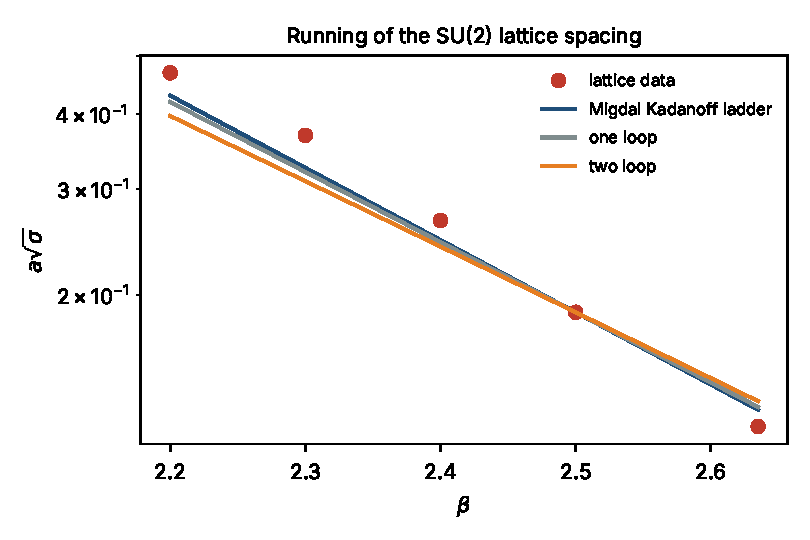
\includegraphics[width=0.85\textwidth]{figures/scaling_test.pdf}
\caption[The Migdal Kadanoff ladder against SU(2) lattice data]{The string tension $a\sqrt\sigma$ of SU(2) with the Wilson action, against the running predicted by the Migdal Kadanoff ladder and by one and two loop perturbation theory, all normalised at $\beta=2.5$.}
\label{fig:scaling}
\end{figure}

The data have a fitted slope of $-3.18$, with local slopes $-2.40$, $-3.27$, $-3.52$ and $-3.25$ between successive couplings (Figure~\ref{fig:scaling}). In this window the lattice spacing therefore shrinks about fifteen percent faster than the ladder predicts, and about twenty five percent faster than two loop perturbation theory. This is the well known failure of asymptotic scaling for the Wilson action at intermediate coupling, which is usually cured by replacing the bare coupling with an effective coupling defined from the measured plaquette, as Parisi proposed~\cite{Pa80}. In its weak coupling limit, $-2.77$, the ladder slope falls between one loop and the data. Its strong coupling corrections, visible in the decrements of Section~\ref{ch:verification}, $0.2623$ at $\beta=2$ rather than $0.25$, slow the running and so push the other way: integrated from the computed decrements the ladder slope is $-2.67$, slightly shallower than one loop and further from the data.

Two conclusions follow. The caricature is not quantitatively accurate at $\beta\approx2.5$, and any comparison theorem for step 4 must allow a bracket of at least this width. And the natural fix is the same as in lattice practice: run the ladder in an effective coupling. Because the ladder carries the whole plaquette law rather than a single number, its own $u_2$, the mean plaquette, supplies such a coupling without further input. The next two sections carry out that test.


\section{The ladder in an effective coupling}

Parisi's effective coupling~\cite{Pa80} replaces the bare $\beta$ by the value $\beta_E$ at which the leading weak coupling formula reproduces the measured plaquette. For SU(2) that formula is $\langle\tfrac12\operatorname{tr}U_p\rangle=1-3/(4\beta)$, so
\[
\beta_E=\frac{3}{4\,(1-\langle\tfrac12\operatorname{tr}U_p\rangle)} .
\]
We measured the plaquette ourselves, with a vectorised checkerboard heat bath of Kennedy and Pendleton type~\cite{KP85} on an $8^4$ lattice, sixty sweeps of equilibration and six hundred of measurement at each coupling. The plaquettes are $0.56997$, $0.60305$, $0.62976$, $0.65264$ and $0.67629$ at $\beta=2.2$, $2.3$, $2.4$, $2.5$ and $2.635$, with standard errors between $1\times10^{-4}$ and $4\times10^{-4}$. The effective couplings are $\beta_E=1.744$, $1.889$, $2.026$, $2.159$ and $2.317$.

\begin{figure}[t]
\centering
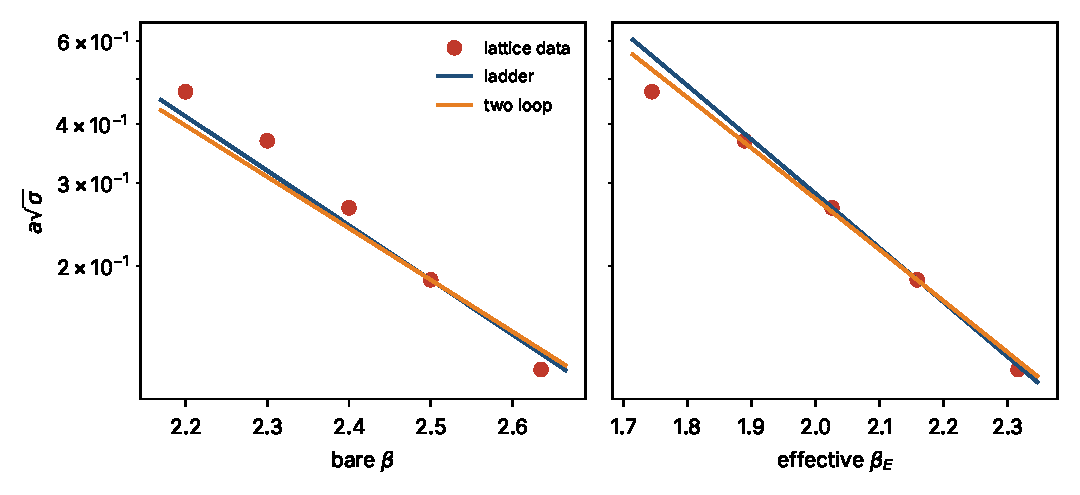
\includegraphics[width=\textwidth]{figures/effective_coupling.pdf}
\caption[The ladder in bare and effective coupling]{SU(2) string tension data against the Migdal Kadanoff ladder and two loop perturbation theory, as functions of the bare coupling (left) and of Parisi's effective coupling (right). The ladder is integrated from the computed decrements $\beta-R(\beta)$, not from their weak coupling limit.}
\label{fig:effcoupling}
\end{figure}

Figure~\ref{fig:plaq4d} places our plaquettes against the strong and weak coupling expansions and the exact two dimensional law.

\begin{figure}[t]
\centering
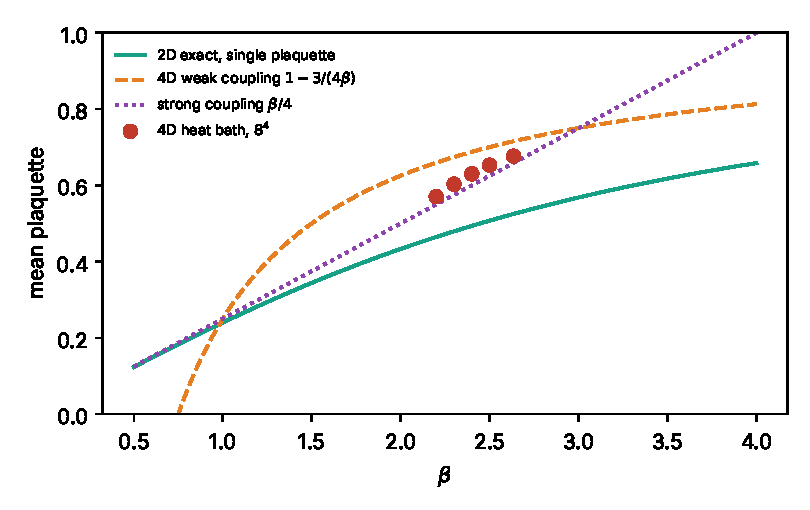
\includegraphics[width=0.85\textwidth]{figures/plaquette_4d.pdf}
\caption[Four dimensional SU(2) plaquette]{Mean plaquette of four dimensional SU(2) from our $8^4$ heat bath runs, against the strong coupling expansion $\beta/4$, the weak coupling formula $1-3/(4\beta)$ that defines $\beta_E$, and the exact single plaquette law of two dimensions.}
\label{fig:plaq4d}
\end{figure}

In the effective coupling the picture changes (Figure~\ref{fig:effcoupling}). The data have slope $-2.40$; two loop perturbation theory gives $-2.48$, within four percent, and the ladder, integrated from its computed decrements $0.268$, $0.265$, $0.263$ and $0.262$ at $\beta=1.5$, $1.7$, $1.9$ and $2.1$, gives $-2.64$, about ten percent too steep. The residual scatter about each prediction is $0.047$ for two loops and $0.066$ for the ladder, against $0.104$ and $0.082$ in the bare coupling. So the effective coupling cures most of the failure of scaling for both, as it does in lattice practice, and the ladder flips from running too slowly, by fifteen percent in the weak coupling slope or nineteen percent in the computed decrements, to ten percent too fast.

\section{The ladder's two loop coefficient}

The remaining discrepancy has a clean source. Write the decrement per doubling of the lattice spacing as $\delta(\beta)=d\beta/d\log_2(1/a)$. Two loop perturbation theory gives
\[
\delta_{\mathrm{pert}}(\beta)=\log2\,\Big(4Nb_0+\frac{8N^2b_1}{\beta}\Big)+O(\beta^{-2})=0.2575+\frac{0.0403}{\beta}+O(\beta^{-2})
\]
for SU(2), with $b_0=11N/(48\pi^2)$ and $b_1=34N^2/(3(16\pi^2)^2)$. The coefficient of $1/\beta$ is unchanged by any shift $\beta\mapsto\beta+c$, which is how a change of scheme acts at this order, so it can be compared across schemes. The ladder at $b=2$ has $\delta_{\mathrm{MK}}(\beta)=0.2500+0.021/\beta$ above $\beta=20$ (Section~\ref{ch:verification}). Figure~\ref{fig:decpert} compares the two decrement curves over the whole range of couplings. The ladder therefore reproduces the one loop coefficient to three percent and the two loop coefficient to about fifty two percent. Its approach to strong coupling is too abrupt: it does not slow down enough as the coupling grows.


\begin{figure}[t]
\centering
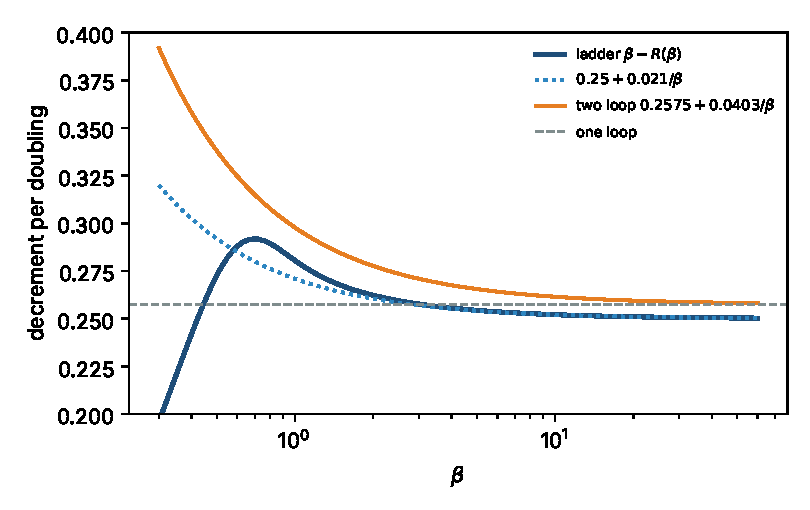
\includegraphics[width=0.85\textwidth]{figures/decrement_vs_pert.pdf}
\caption[Ladder decrement against perturbation theory]{The computed ladder decrement $\beta-R(\beta)$ at $b=2$, its fit $0.25+0.021/\beta$, and the two loop perturbative decrement $0.2575+0.0403/\beta$. The ladder tends to $0.25$, three percent below one loop, with about half the two loop coefficient of $1/\beta$, and peaks near $\beta=0.7$ before falling at strong coupling.}
\label{fig:decpert}
\end{figure}

\begin{quote}
\textsc{Status.} In Parisi's effective coupling the ladder predicts the running of the SU(2) string tension over $2.2\le\beta\le2.635$ to within ten percent; two loop perturbation theory does better, to four percent. The ladder's own two loop coefficient is $0.021$ against the true $0.0403$. Any comparison theorem for step 4 must therefore allow a bracket that corrects the second order running, and an improved ladder, for example with $b$ varied along the flow or with the bond moving step weighted by the measured plaquette, should first be tested on this coefficient.
\end{quote}

\section{Can the scale factor repair the ladder?}

The ladder has one free parameter, the scale factor $b$, which need not be an integer: bond moving raises the plaquette law to the power $b^2$ and decimation raises character coefficients to the power $b^2$, and both make sense for real $b>1$. Per doubling of the lattice spacing the decrement is $a(b)+c(b)/\beta$ with
\[
a(b)=\frac{1-b^{-2}}{3\log_2b},
\]
from Remark~\ref{prop:decrementB}. We computed $c(b)$ by fitting the decrement on $20\le\beta\le150$; the fitted $a(b)$ agrees with the formula to five digits.

\begin{center}
\small
\begin{tabular}{cccccccccc}
\toprule
$b$ & 1.2 & 1.4 & 1.6 & 1.8 & 1.925 & 2 & 2.2 & 3 \\ \midrule
$a(b)$ & 0.387 & 0.336 & 0.300 & 0.272 & 0.2576 & 0.250 & 0.232 & 0.187 \\
$c(b)$ & 0.090 & 0.057 & 0.039 & 0.028 & 0.0232 & 0.0208 & 0.016 & 0.007 \\
\bottomrule
\end{tabular}
\end{center}

\begin{figure}[t]
\centering
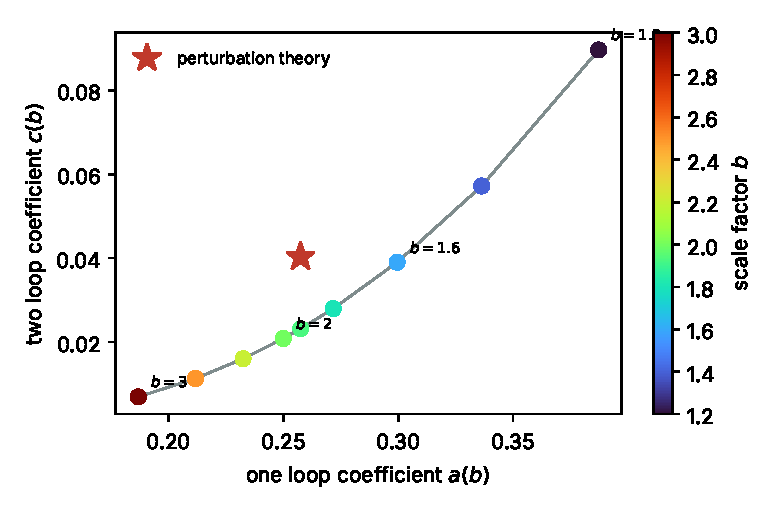
\includegraphics[width=0.8\textwidth]{figures/ladder_b.pdf}
\caption[One and two loop coefficients of the ladder as the scale factor varies]{The one loop and two loop coefficients $(a(b),c(b))$ of the ladder as the scale factor $b$ varies, coloured by $b$, and the perturbative values $(0.2575,0.0403)$, marked by a star. The curve passes below the star: no scale factor matches both.}
\label{fig:ladderb}
\end{figure}

At $b=2$ the two loop coefficient is $0.02083$, which is $1/48$ to the accuracy of the fit; the next section proves it. The scale factor $b_*=1.925$ reproduces the one loop coefficient $0.2575$ exactly, and there $c=0.0232$, still fifty eight percent of the true $0.0403$. Matching the coefficient $c$ itself instead needs $b=1.58$, where the one loop coefficient is seventeen percent too large. Figure~\ref{fig:ladderb} shows the curve $(a(b),c(b))$ passing below the perturbative point. The scale factor alone cannot repair the ladder; the second order error is structural, a property of bond moving, and an improved ladder must change the bond moving step itself.

\section{The weak coupling expansion of the ladder, exactly}

The numerical value $c(2)=0.02083$ of the last section suggested $1/48$. The whole expansion can in fact be computed in closed form, and the scale factor enters through one rational function.

\begin{theorem}[weak coupling expansion]\label{thm:expansion}
Let bond moving have power $k$ and decimation power $D$, and let $t=2/\beta$ be the heat kernel time. For SU(2) the projected ladder map is, as $t\to0$,
\[
t'=\frac{D}{k}\,t\,\Big[1+\Big(1-\frac1k\Big)\Big(\frac t6+\frac{t^2}{36}\Big)+\frac{(k-1)(2k^2+2k-3)}{432\,k^3}\,t^3+O(t^4)\Big].
\]
In four dimensions, $k=D=b^2$, the decrement is
\[
\beta-R(\beta)=\frac{b^2-1}{3b^2}+\frac{b^2-1}{9b^4}\,\frac1\beta+\frac{(b^2-1)(2b^2-1)}{54\,b^6}\,\frac1{\beta^2}+O(\beta^{-3}),
\]
which for $b=2$ is $\frac14+\frac{1}{48\beta}+\frac{7}{1152\beta^2}$.
\end{theorem}

\begin{proof}
For small $t$ the heat kernel is its leading image up to terms of relative size $e^{-4\pi^2/t}$ away from the antipode, and the antipode carries exponentially small mass: $K_t(\theta)\propto(\theta/\sin\theta)\,e^{-\theta^2/t}$. After bond moving the law of the angle has density proportional to
\[
K_t(\theta)^k\sin^2\theta\ \propto\ \theta^2\Big(\frac{\theta}{\sin\theta}\Big)^{k-2}e^{-\theta^2/\tau},\qquad\tau=\frac tk .
\]
This is the radial law of a Gaussian vector in $\R^3$ with a weight $w=\exp\big((k-2)\log(\theta/\sin\theta)\big)$, and $\log(\theta/\sin\theta)=\theta^2/6+\theta^4/180+\theta^6/2835+\cdots$. The new coefficient is $u_2=\E[w\cos\theta]/\E[w]$, where both expectations are polynomials in $\tau$ at each order because the moments of $\theta^2e^{-\theta^2/\tau}$ are $\E\theta^{2j}=\tau^j\,\Gamma(j+\frac32)/\Gamma(\frac32)$. Decimation gives $t'=-\frac43D\log u_2$. Expanding to the stated order is a finite computation, done in exact rational arithmetic by the script of Appendix~\ref{ch:code}.
\end{proof}

The case $k=2$ can be done by hand and checks the series. The weight is then one, the law is exactly the radial Gaussian, and $\E\cos|X|=(1-\sigma^2)e^{-\sigma^2/2}$ with $\sigma^2=t/4$, so $t'=D\big[\frac t6-\frac43\log(1-\frac t4)\big]=D\big[\frac t2+\frac{t^2}{24}+\frac{t^3}{144}+\cdots\big]$, in agreement with the theorem. The theorem also agrees with the numerical decrements of Section~\ref{ch:verification}: at $b=2$ it gives $0.25441$ at $\beta=5$ and $0.2521$ at $\beta=10$, against the computed $0.2544$ and $0.2521$.

Three consequences.

First, the leading term is Remark~\ref{prop:decrementB}, with $\E S_{\mathrm{BPY}}=\frac13$ appearing as twice the coefficient $\frac16$ of $\theta^2$ in $\log(\theta/\sin\theta)$. The higher coefficients $\frac1{180}$ and $\frac1{2835}$, multiplied by $2^jj!$ for the coefficient of $\theta^{2j}$, are, up to such factors, the higher cumulants of the Biane, Pitman and Yor variable~\cite{BPY}. The expansion of the ladder is the cumulant expansion of $S_{\mathrm{BPY}}$.

Second, the comparison with perturbation theory can be made in a form that does not depend on the scheme. Write one step as $t'=t+At^2+A't^3$. For a flow $\mathrm dt/\mathrm d\log a=\alpha t^2(1+\rho t)$ integrated over a scale factor, $(A'-A^2)/A=\rho$, and $\rho$ is invariant under $t\mapsto t+ct^2$. The true theory has $\rho=2b_1/b_0=17N/(44\pi^2)$, which is $0.0783$ for SU(2). The ladder has
\[
\rho_{\mathrm{ladder}}=\frac{A'-A^2}{A}=\frac{1}{6b^2},
\]
which is $0.0417$ at $b=2$, fifty three percent of the truth. The two values of $\rho$ agree at $b=1.459$, where the one loop coefficient is twenty six percent too large; at $b=1.925$, where one loop is exact, $\rho_{\mathrm{ladder}}=0.0450$. The curve of Figure~\ref{fig:ladderb} is now explicit, and the statement that no scale factor matches both coefficients is a theorem: one needs $(1-b^{-2})/(3\log_2b)=0.2575$ and $1/(6b^2)=0.0783$ at once.

Third, the infinitesimal ladder exists. As $b\to1$ the step becomes the flow $\mathrm dt/\mathrm d\log b=\frac{t^2}{3}\big(1+\frac t6+\cdots\big)$, whose one loop coefficient is $1.79$ times the true one. The Migdal Kadanoff approximation is not improved by making the steps small; its accuracy at $b=2$ is an accident of that scale factor; for the approximation itself see~\cite{Mi75,Ka76}.

In $d$ dimensions the same theorem, with $k=b^{d-2}$ and $D=b^2$, gives $t'=b^{4-d}t\,[1+(1-b^{2-d})(t/6+t^2/36)+\cdots]$. In three dimensions the time grows by the factor $b$ at every step and the curvature terms are corrections; in two they vanish identically and the map is exact.

\section{The expansion for SU(N)}

The same computation can be done on the maximal torus of SU(N). At small time the heat kernel is $\prod_{i<j}J(\phi_i-\phi_j)\,e^{-|\phi|^2/(2t)}$ with $J(x)=(x/2)/\sin(x/2)$, the Haar density is $\prod_{i<j}\sin^2((\phi_i-\phi_j)/2)$, and after bond moving the law on the torus is a Gaussian on the Lie algebra, in radial form, with the weight $\prod_{i<j}J(\phi_i-\phi_j)^{k-2}$. Normalise the time by $u_F=e^{-C_Ft}$ for the fundamental character, with $C_F=(N^2-1)/(2N)$, so that $\beta=2N/g^2=N/t$.

\begin{theorem}\label{thm:expansionN}
For every $N\ge2$ the projected ladder map is
\[
t'=\frac Dk\,t\,\Big[1+\Big(1-\frac1k\Big)\Big(\frac{Nt}{12}+\Big(\frac{Nt}{12}\Big)^2\Big)+O(t^3)\Big],
\]
so that in four dimensions, with $k=D=b^2$,
\[
\beta-R(\beta)=\frac{N^2}{12}\Big(1-\frac1{b^2}\Big)+\frac{N^4}{144\,b^2}\Big(1-\frac1{b^2}\Big)\frac1\beta+O(\beta^{-2}),
\]
and the two loop ratio of the ladder is $\rho_{\mathrm{ladder}}=N/(12b^2)$.
\end{theorem}

\begin{proof}
Let $X$ be the element of the Lie algebra with eigenvalues $i\phi_j$, so that the torus law is the radial part of a law on $\mathfrak{su}(N)$, of dimension $n=N^2-1$, and write $p_r=\sum_j\phi_j^r$, with $p_1=0$. Put $\tau=t/k$ and $m=k-2$. Since $\log J(x)=x^2/24+x^4/2880+\cdots$ and $\sum_{i\ne j}(\phi_i-\phi_j)^2=2Np_2$, $\sum_{i\ne j}(\phi_i-\phi_j)^4=2Np_4+6p_2^2$, the weight is $\exp\big(m(L_2+L_4+\cdots)\big)$ with
\[
L_2=\frac{N}{24}\,p_2,\qquad L_4=\frac{2Np_4+6p_2^2}{5760}.
\]
The factor $e^{mL_2}$ is Gaussian: it changes the variance from $\tau$ to $\tau_{\mathrm e}=\tau/(1-mN\tau/12)$. Let $g(\tau)=\log\E_\tau[\chi_F/N]$ under the Gaussian law of variance $\tau$ on the Lie algebra, and write $g(\tau)=-C_F\tau(1+\mu_1\tau+\mu_2\tau^2+\cdots)$. To first order in $L_4$, which is all that contributes at order $\tau^3$,
\[
\log u_F=g(\tau_{\mathrm e})+m\operatorname{Cov}_\tau\Big(L_4,-\frac{p_2}{2N}\Big)+O(\tau^4).
\]
Under the Gaussian law $p_2/\tau$ is chi squared with $n$ degrees of freedom, so $\operatorname{Cov}(p_2^2,p_2)=4n(n+2)\tau^3$. The direction of $X$ is independent of its length, so $\operatorname{Cov}(p_4,p_2)=4\tau\,\E p_4$, and for traceless Hermitian Gaussian matrices $\E p_4=\tau^2(N^2-1)(2N^2-3)/N$, from the fourth moment $(2N^3+N)\tau^2$ of the Gaussian unitary ensemble after removing the trace. Hence
\begin{align*}
m\operatorname{Cov}\Big(L_4,-\frac{p_2}{2N}\Big)&=-\frac{m\,n\,\tau^3}{2N\cdot5760}\,\big[8(2N^2-3)+24(N^2+1)\big]\\
&=-C_F\,\frac{mN^2\tau^3}{144}.
\end{align*}
The coefficients $\mu_1,\mu_2$ are fixed by the case $k=1$, where the law is the heat kernel itself and $\log u_F=-C_F\tau$ exactly: with $m=-1$ this forces $\mu_1=N/12$ and $\mu_2=N^2/72$. Substituting, with $s=N\tau/12$,
\begin{align*}
\log u_F&=-C_F\tau\,\big[1+(m+1)s+(m+1)(m+2)s^2\big]+O(\tau^4)\\
&=-C_F\tau\,\big[1+(k-1)s+k(k-1)s^2\big]+O(\tau^4),
\end{align*}
and $t'=-D\log u_F/C_F$ is the stated map.
\end{proof}

The values $\mu_1=N/12$ and $\mu_2=N^2/72$ can be checked for $N=2$, where $g(\tau)=-\frac\tau4+\log(1-\frac\tau2)$. The whole theorem was first found, and is confirmed for $N=2$, $3$ and $4$, by exact integration against the squared Vandermonde weight on the torus, with the script in Appendix~\ref{ch:code}; for $N=3$ and $b=2$ the leading term is the decrement $9/16$ of the full numerical flow.

The dependence on $N$ is the notable point. The true two loop ratio is $2b_1/b_0=17N/(44\pi^2)$, also linear in $N$. Hence
\[
\frac{\rho_{\mathrm{ladder}}}{\rho_{\mathrm{true}}}=\frac{11\pi^2}{51\,b^2},\qquad\frac{\text{one loop, ladder}}{\text{one loop, true}}=\frac{\pi^2(1-b^{-2})}{11\log b},
\]
and neither depends on $N$. At $b=2$ they are $0.532$ and $0.971$ for every gauge group SU(N). The ladder has the correct dependence on $N$ at one and two loops, the planar scaling in which $\beta/N^2$ is the natural variable, and its defects are pure numbers. In the variable $x=Nt/12$ the ladder is one map for all $N$: $x'=\frac Dkx[1+(1-\frac1k)(x+x^2)+\cdots]$. Whatever is missing from the Migdal Kadanoff approximation is missing uniformly in $N$, and so cannot be a $1/N$ effect.

\section{The local heat kernel time, and the Wilson start}

Corollary~\ref{cor:mlrall} has a use beyond monotonicity of $R$. Because the score $\partial_\theta\log K_t(\theta)$ is strictly increasing in $t$ at every angle, from $-\infty$ as $t\to0$ to $0$ as $t\to\infty$, any class function law $f$ with negative score has a well defined local heat kernel time
\[
t_f(\theta)=\text{the unique }t\text{ with }\partial_\theta\log K_t(\theta)=\partial_\theta\log f(\theta).
\]

\begin{proposition}\label{prop:localtime}
Let $t_-=\inf_\theta t_f(\theta)$ and $t_+=\sup_\theta t_f(\theta)$. Then $K_{t_-}\le_{\mathrm{lr}}f\le_{\mathrm{lr}}K_{t_+}$, these are the tightest heat kernel bounds in the likelihood ratio order, and $f$ is a heat kernel law exactly when $t_f$ is constant. Bond moving preserves the bracket, with $t_\pm$ computed for the powers. Convolution with a heat kernel preserves the likelihood ratio order between class function laws.
\end{proposition}

\begin{proof}
The logarithmic derivative of $K_{t_+}/f$ is $\partial_\theta\log K_{t_+}-\partial_\theta\log f\ge0$ by the definition of $t_+$ and the monotonicity of the score, so the ratio is increasing; similarly for $t_-$. Powers multiply scores by $k$ and so preserve the order of scores. For the last statement, the angle of Brownian motion on SU(2) is a one dimensional diffusion on $[0,\pi]$, and by the theorem of Karlin and McGregor~\cite{KM59} its transition density is totally positive; a kernel that is totally positive of order two preserves the likelihood ratio order.
\end{proof}

The ratio $t_+/t_-$ measures the distance of a law from the heat kernel family in the order that the ladder respects. We followed it along the ladder started from the Wilson law at $\beta=2.5$ (Figure~\ref{fig:localtime}).

\begin{center}
\small
\begin{tabular}{cccccccc}
\toprule
rung & 0 & 1 & 2 & 3 & 4 & 5 & 6 \\ \midrule
$t_-$ & 0.707 & 0.824 & 0.928 & 1.055 & 1.224 & 1.459 & 1.812 \\
$t_+$ & 1.788 & 0.913 & 0.939 & 1.062 & 1.232 & 1.470 & 1.830 \\
$t_+/t_-$ & 2.530 & 1.107 & 1.012 & 1.006 & 1.007 & 1.008 & 1.010 \\
\bottomrule
\end{tabular}
\end{center}

\begin{figure}[t]
\centering
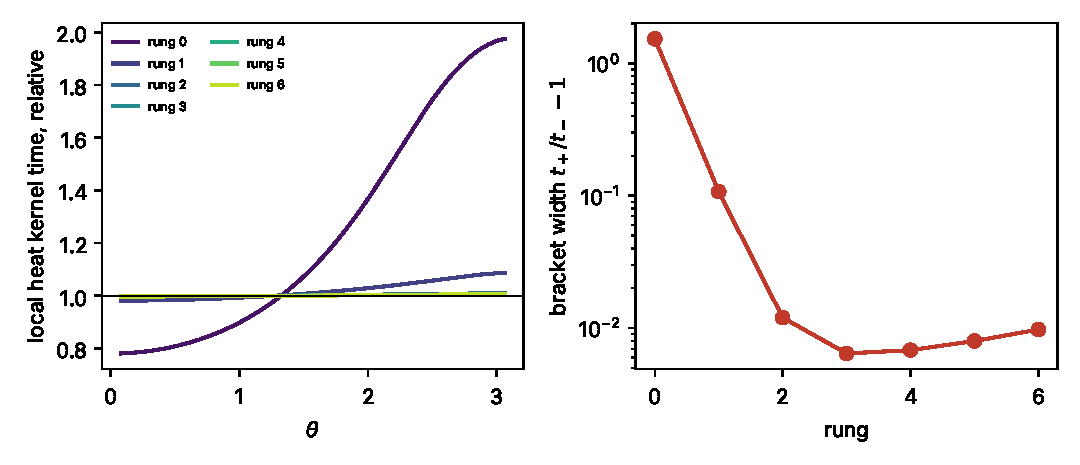
\includegraphics[width=\textwidth]{figures/local_time.pdf}
\caption[The local heat kernel time along the ladder]{Left: the local heat kernel time $t_f(\theta)$ of the plaquette law at each rung of the ladder started from the Wilson law at $\beta=2.5$, relative to the time defined by $u_2$. A heat kernel law is a horizontal line at one. Right: the width $t_+/t_--1$ of the heat kernel bracket in the likelihood ratio order.}
\label{fig:localtime}
\end{figure}

The Wilson law itself is far from the family: its local time ranges over a factor of $2.5$, short near the identity and long near the antipode, which is Proposition~\ref{prop:wilsonflow} seen pointwise. One step of the ladder cuts the width to eleven percent and a second to $1.2$ percent, after which it stays between $0.6$ and one percent. So the ladder started from the Wilson action enters a one percent neighbourhood of the heat kernel family, in the likelihood ratio order, after two rungs, and stays there through the six rungs computed. The neighbourhood does not shrink to zero: the invariant manifold of the ladder is close to the heat kernel family but is not equal to it, which is the residual error of the projection in Section~\ref{ch:verification}.

This answers the question of how to extend the monotone covering from heat kernel starts to Wilson starts: carry the pair $(t_-,t_+)$ instead of a single time. For that to be a theorem, decimation, the convolution of a law with itself, must preserve the likelihood ratio order when the law is not a heat kernel. The next section settles when it does.

\section{When does convolution preserve the likelihood ratio order?}

Let $f$ be a class function density on SU(2), and let $X$ have angle $\theta'$ and $Y$ be independent with law $f$. The angle $\psi$ of $XY$ satisfies $\cos\psi=\cos\alpha\cos\theta'-\sin\alpha\sin\theta'\cos\xi$, with $\alpha$ the angle of $Y$ and $\cos\xi$ uniform on $[-1,1]$, so the transition density from $\theta'$ to $\psi$ is
\[
q_f(\theta',\psi)=\frac{\sin\psi}{\pi\sin\theta'}\,F(\theta',\psi),\qquad F(x,y)=\int_{|x-y|}^{\min(x+y,\,2\pi-x-y)}w(\alpha)\,\mathrm d\alpha,
\]
where $w=f\sin$.
The kernel $q_f$ is totally positive of order two exactly when $F$ is.

\begin{theorem}[total positivity of convolution]\label{thm:tp2}
Let $w=f\sin$ be positive and twice differentiable on $(0,\pi)$, and put
\[
Q(\alpha)=\frac{w''(\alpha)}{w(\alpha)}=\frac{\Delta f}{f}(\alpha)-1,\qquad\Delta=\partial_\alpha^2+2\cot\alpha\,\partial_\alpha ,
\]
with $\Delta$ the radial Laplacian of the three sphere. If $Q$ is nondecreasing on $(0,\pi)$, then $F$ is totally positive of order two, and convolution with $f$ preserves the likelihood ratio order between class function laws. If $Q$ is nonincreasing, $F$ is reverse regular of order two. Equality holds throughout exactly when $w''=\lambda w$.
\end{theorem}

\begin{proof}
For $x\ge y$ with $x+y\le\pi$ put $a=x-y$, $b=x+y$ and $H=\int_a^bw$. Then $F_x=w(b)-w(a)$, $F_y=w(b)+w(a)$, $F_{xy}=w'(b)+w'(a)$, and
\[
\Psi(a,b):=F\,F_{xy}-F_xF_y=H\,\big(w'(a)+w'(b)\big)-w(b)^2+w(a)^2 .
\]
For $x+y>\pi$ the upper limit is $c=2\pi-x-y$, and the same computation gives $FF_{xy}-F_xF_y=\Psi(a,c)$. So $F$ is totally positive of order two if and only if $\Psi(a,b)\ge0$ for all $0<a<b<\pi$; $F$ is continuously differentiable across the lines $x=y$ and $x+y=\pi$ because $w$ vanishes at $0$ and $\pi$. Now
\begin{align*}
\partial_b\Psi&=w(b)\big(w'(a)-w'(b)\big)+H\,w''(b),\\
\partial_a\Psi&=w(a)\big(w'(a)-w'(b)\big)+H\,w''(a),
\end{align*}
and therefore
\[
\Big(\frac{1}{w(b)}\partial_b-\frac{1}{w(a)}\partial_a\Big)\Psi=H\,\big(Q(b)-Q(a)\big).
\]
In the coordinates $u=\int_0^bw$ and $v=\int_0^aw$ the left side is $(\partial_u-\partial_v)\Psi$. On the diagonal $u=v$, $\Psi=0$. Moving from the diagonal in the direction $(1,-1)$, which widens the interval $[a,b]$, the derivative of $\Psi$ is $(u-v)(Q(b)-Q(a))$, which is nonnegative when $Q$ is nondecreasing. Hence $\Psi\ge0$. The other cases are the same argument with the sign reversed.
\end{proof}

The equality cases are the laws with $\Delta f=(\lambda+1)f$: Haar measure and, formally, the single characters, for which the convolution kernel factorises. The condition has a second reading. Under the heat flow, $4\partial_t\log\rho=\Delta\rho/\rho$, so
\[
\partial_\alpha\,\frac{\Delta\rho}{\rho}=4\,\partial_t\partial_\alpha\log\rho .
\]
The hypothesis of Theorem~\ref{thm:tp2} is that $f$, as an initial law for the heat flow, has monotone likelihood ratio in time at time zero. Three corollaries follow at once.

\begin{corollary}\label{cor:tp2}
\begin{enumerate}
\item[(i)] Every heat kernel $K_t$ satisfies the hypothesis, by Corollary~\ref{cor:mlrall}. This is an independent proof, from the product formula, of the total positivity of order two of the radial heat semigroup on SU(2).
\item[(ii)] The Wilson law $e^{\kappa\cos\theta}$ satisfies it if and only if $\kappa\le3/2$, by Proposition~\ref{prop:wilsonflow}.
\item[(iii)] The hypothesis is preserved by the heat flow, by the maximum principle of Section~\ref{ch:proofs2} of the appendix, and the class of laws whose convolution kernels are totally positive of order two is closed under convolution, because such kernels compose.
\end{enumerate}
\end{corollary}

So if $f_1\le_{\mathrm{lr}}f_2$ and both have totally positive kernels, then $f_1^{*m}\le_{\mathrm{lr}}f_2^{*m}$ for every $m$: replace the factors one at a time. Decimation is monotone in the likelihood ratio order on that class.

One might ask whether log concavity in $\cos\theta$ is enough. It is not. Bond moved laws $K_t^k$ are log concave in $\cos\theta$ by Corollary~\ref{cor:logconc}, but
\[
\partial_\alpha\frac{\Delta(f^k)}{f^k}=k\,\partial_\alpha\frac{\Delta f}{f}+2k(k-1)\,v\,v',\qquad v=\partial_\alpha\log f,
\]
and near the antipode $v<0$ and $v'>0$, so the second term is negative and, for $k=4$, wins. A direct evaluation of $\Psi$ on a grid of pairs confirms it.

\begin{center}
\small
\begin{tabular}{lcc}
\toprule
law & share of pairs $(a,b)$ with $\Psi<0$ & where \\ \midrule
$K_2$ & 0 & \\
Wilson, $\kappa=1.4$ & 0 & \\
Wilson, $\kappa=2.5$ & 0.13 & $b$ near $\pi$ \\
$K_2^4$ & 0.06 & $b$ near $\pi$ \\
$K_1^4$ & 0.04 & $b$ near $\pi$ \\
\bottomrule
\end{tabular}
\end{center}

The violations are confined to pairs whose upper end is at the antipode, where the law has exponentially little mass at weak coupling. The conclusion, numerical for bond moved laws, is this: decimation of heat kernel laws is monotone in the likelihood ratio order; decimation of bond moved laws is monotone wherever total positivity holds, and total positivity fails only at the antipode. In the language of the renormalization group that is the large field region, which Ba\l aban's small field analysis~\cite{Ba87} leaves to a separate treatment. The comparison of Section~\ref{ch:isthere} should therefore be posed in the likelihood ratio order on a ball around the identity, together with a bound on the mass outside it.

\section{The bad cap at the antipode}

The failure can be located exactly. For $f=K_t^k$, the product formula gives, with $c=\cos\alpha$, $S_1=\sum_m(\gamma_m+c)^{-1}$ and $S_2=\sum_m(\gamma_m+c)^{-2}$,
\[
\partial_\alpha\frac{\Delta(K_t^k)}{K_t^k}=k\sin\alpha\,\Big[4\sum_m\frac{\gamma_m'(t)}{(\gamma_m+c)^2}+2(k-1)\,S_1\big(c\,S_1+(1-c^2)S_2\big)\Big].
\]

\begin{theorem}[the near hemisphere]\label{thm:hemisphere}
For every $t>0$ and every $k\ge1$ the bond moved law $K_t^k$ satisfies the hypothesis of Theorem~\ref{thm:tp2} on $(0,\pi/2]$. Consequently $\Psi(a,b)\ge0$ whenever $b\le\pi/2$, and the kernel of convolution with $K_t^k$ is totally positive of order two on the set of pairs of angles with $\theta'+\psi\le\pi/2$.
\end{theorem}

\begin{proof}
For $c\ge0$ every term in the bracket is nonnegative, since $\gamma_m>1$, $\gamma_m'>0$ and $S_1,S_2>0$. The argument of Theorem~\ref{thm:tp2} uses the monotonicity of $Q$ only on the interval $[a,b]$.
\end{proof}

Beyond the hemisphere the bracket stays positive until an angle $\alpha_*(t,k)=\pi-\eta(t,k)$. From the leading image, $v\approx-2\alpha/t$ and $v'\approx\sin^{-2}\alpha-\alpha^{-2}-2/t$, and the bracket changes sign where $\sin^{-2}\alpha-\alpha^{-2}=2k/((k-1)t)$, so
\[
\eta(t,k)\approx\sqrt{\frac{(k-1)\,t}{2k}}\qquad(t\to0).
\]
We computed $\eta$ from the image sum, and the mass that the bond moved law gives to the cap of radius $\eta$ at the antipode (Figure~\ref{fig:antipode}).

\begin{center}
\small
\begin{tabular}{ccccc}
\toprule
 & \multicolumn{2}{c}{$k=4$, four dimensions} & \multicolumn{2}{c}{$k=2$, three dimensions} \\
$t$ & $\eta$ (prediction) & mass of cap & $\eta$ (prediction) & mass of cap \\ \midrule
0.1 & 0.192 (0.194) & $10^{-148}$ & 0.154 (0.158) & $10^{-77}$ \\
0.2 & 0.271 (0.274) & $4.5\times10^{-69}$ & 0.214 (0.224) & $6.3\times10^{-37}$ \\
0.4 & 0.381 (0.387) & $10^{-31}$ & 0.294 (0.316) & $10^{-17}$ \\
0.8 & 0.528 (0.548) & $3\times10^{-13}$ & 0.372 (0.447) & $2\times10^{-8}$ \\
1.6 & 0.657 (0.775) & $2\times10^{-5}$ & 0.165 & $10^{-5}$ \\
\bottomrule
\end{tabular}
\end{center}

\begin{figure}[t]
\centering
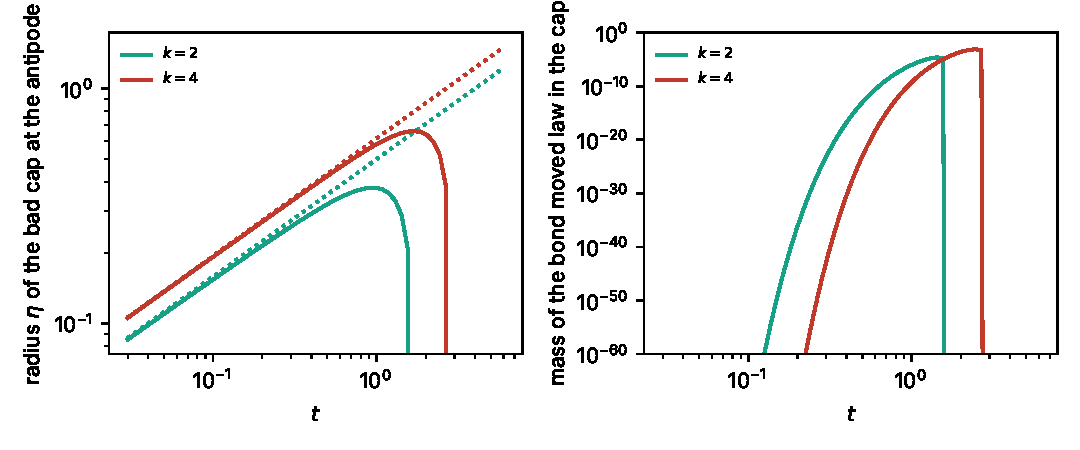
\includegraphics[width=\textwidth]{figures/antipode_radius.pdf}
\caption[The bad cap at the antipode]{Left: the radius $\eta$ of the cap at the antipode on which the bond moved law $K_t^k$ fails the total positivity condition, with the small time prediction $\sqrt{(k-1)t/(2k)}$ dotted. The cap closes at $t=2.88$ for $k=4$ and at $t=1.67$ for $k=2$. Right: the mass of the bond moved law in the cap.}
\label{fig:antipode}
\end{figure}

Three facts stand out. The small time formula is accurate to a few percent up to $t=0.8$ for $k=4$ and up to $t=0.2$ for $k=2$. The cap disappears entirely at strong coupling, according to the computed $\eta$: for $t\ge2.88$ with $k=4$, that is $\beta\le0.69$, and for $t\ge1.67$ with $k=2$, the bond moved law appears to satisfy the condition on the whole group and decimation to be monotone without qualification. This rests on the numerical $\eta$ and is not proved. And in between the cap never carries much mass: its mass is largest, $8\times10^{-4}$, at $t=2.47$ for $k=4$, and $2\times10^{-5}$ at $t=1.45$ for $k=2$. At the couplings of lattice simulations, $\beta\ge2.2$, it is below $10^{-10}$ for $k=4$.

A failure of total positivity on a set of small mass costs a small error.

\begin{proposition}[truncated monotonicity]\label{prop:truncated}
Let $q(\theta',\psi)\le M$ be a transition density that is totally positive of order two on $[0,A]\times[0,L]$, and let $f_1\le_{\mathrm{lr}}f_2$ be probability densities on $[0,\pi]$ with masses $\varepsilon_1,\varepsilon_2$ beyond $A$. Then for $\psi_1<\psi_2\le L$,
\[
(qf_2)(\psi_2)\,(qf_1)(\psi_1)-(qf_2)(\psi_1)\,(qf_1)(\psi_2)\ \ge\ -M^2\,(\varepsilon_1+\varepsilon_2+\varepsilon_1\varepsilon_2),
\]
where $(qf)(\psi)=\int f(\theta')q(\theta',\psi)\,\mathrm d\theta'$.
\end{proposition}

\begin{proof}
Split each integral at $A$. The parts over $[0,A]$ satisfy the inequality with zero on the right, by the basic composition formula, since $f_1$ and $f_2$ restricted to $[0,A]$ are still ordered and $q$ is totally positive there. Each tail is at most $M\varepsilon$ and each truncated integral at most $M$; dropping the tails from the first product and bounding them in the second gives the error term.
\end{proof}

With $A+L\le\pi/2$ the kernel of convolution with $K_t^k$ qualifies, by Theorem~\ref{thm:hemisphere}. So one step of the ladder is monotone in the likelihood ratio order on the ball of radius $L$, up to an error of at most $M^2(\varepsilon_1+\varepsilon_2+\varepsilon_1\varepsilon_2)$, with $\varepsilon_i$ the masses outside the ball of radius $A$. With $A=L=\pi/4$ the mass outside is of order $e^{-k\pi^2/(16t)}$, which is $0.05$ at $\beta=2.5$ and $4\times10^{-6}$ at $\beta=10$ for $k=4$. If the numerically determined $\eta$ is used, so that $A+L\le\pi-\eta$ and $A=L$ is just below $\pi/2$, the mass is of order $e^{-k\pi^2/(4t)}$, which is $4\times10^{-6}$ at $\beta=2.5$ and $4\times10^{-22}$ at $\beta=10$; this version is numerical. At strong coupling the cap appears, numerically, to be absent and the step monotone exactly.

\begin{quote}
\textsc{Status.} Decimation is monotone in the likelihood ratio order for heat kernel laws at every coupling; for bond moved laws on the near hemisphere, with an error that is exponentially small at weak coupling; and, numerically and not yet proved, for bond moved laws at strong coupling, $\beta\le0.69$ in four dimensions. The window $0.7<\beta<2$, together with the couplings just above $2$ where the error bound of Proposition~\ref{prop:truncated} is not yet small, and where the law is spread over the whole group and the cap has mass up to $8\times10^{-4}$, is what remains. It is the crossover, again.
\end{quote}

\section{The ladder contracts: a proof}\label{sec:contracts}\index{Hamilton, R. S.}\index{Harnack inequality}\index{maximum principle}

The inequality $R(\beta)<\beta$ of Section~\ref{ch:verification} was verified on a grid. It can be proved. The idea is to compare the bond moved law $K_t^k$ not with $K_t$ but with the heat kernel at the time flat space would give, $K_{t/k}$.

Write $x=\cos\theta$ and $G(t,x)=\partial_x\log K_t$. In flat space $\log K_t=-\theta^2/t$ and $t\,\partial_\theta\log K_t$ does not depend on $t$: the $k$th power of a Gaussian is the Gaussian at time $t/k$, and bond moving followed by decimation returns the starting time in four dimensions. On the group the same quantity moves, and it moves one way.

\begin{theorem}[time scaled likelihood ratio]\label{thm:scaledmlr}
For the SU(2) heat kernel with $u_2=e^{-3t/4}$, the function $t\,\partial_x\log K_t(x)$ is strictly decreasing in $t$ on $t>0$, for every $x\in[-1,1]$.
\end{theorem}

\begin{proof}
Three steps, with $t_1=0.1$.

\emph{Step 1, an equation.} Put $\phi=\log K_t$, $v=t\,\partial_\theta\phi$ and $z=\partial_tv$. Since $\partial_x=-(\sin\theta)^{-1}\partial_\theta$, the claim is $z>0$ on $(0,\pi)$. From $\partial_t\phi=\frac14\big(\phi''+\phi'^2+2\cot\theta\,\phi'\big)$, differentiating once in $\theta$ and once in $t$,
\[
\partial_tz=\tfrac14z''+\Big(\frac{v}{2t}+\frac{\cot\theta}{2}\Big)z'+\Big(\frac1t\Big(1+\frac{t\phi''}{2}\Big)-\frac{1}{2\sin^2\theta}\Big)z+\frac{-v}{t^2}\Big(1+\frac{t\phi''}{2}\Big).
\]
In flat space $t\phi''=-2$ and the last term, the source, vanishes.

\emph{Step 2, the source is nonnegative.} By the product formula $K_t$ is increasing in $x$, so $-v\ge0$. Hamilton's matrix Harnack inequality~\cite{Ha93} states that on a compact manifold with nonnegative sectional curvature and parallel Ricci tensor every positive solution of $\partial_\varsigma u=\Delta u$ satisfies $\nabla^2\log u+\mathbf m/(2\varsigma)\ge0$, with $\mathbf m$ the metric. The round sphere $S^3$ qualifies, our time is $\varsigma=t/4$, and the radial component of the Hessian is $\phi''$; hence $1+t\phi''/2\ge0$. So the source is nonnegative, and $z$ is a supersolution of a linear parabolic equation whose coefficient of $z$ is bounded above on $t\ge t_1$. The function $z$ vanishes at $\theta=0$ and $\theta=\pi$, where $v$ vanishes by symmetry. By the maximum principle, applied to $e^{-\lambda t}z$ with $\lambda$ larger than that bound, $z(t_1,\cdot)\ge0$ implies $z(t,\cdot)\ge0$ for all $t\ge t_1$, and the strong maximum principle makes the inequality strict on $(0,\pi)$.

\emph{Step 3, the initial layer.} It remains to show $z(t,\cdot)>0$ for $0<t\le t_1$. This is Proposition~\ref{prop:initial} below, an explicit estimate with the images of the heat kernel.
\end{proof}

\begin{figure}[t]
\centering
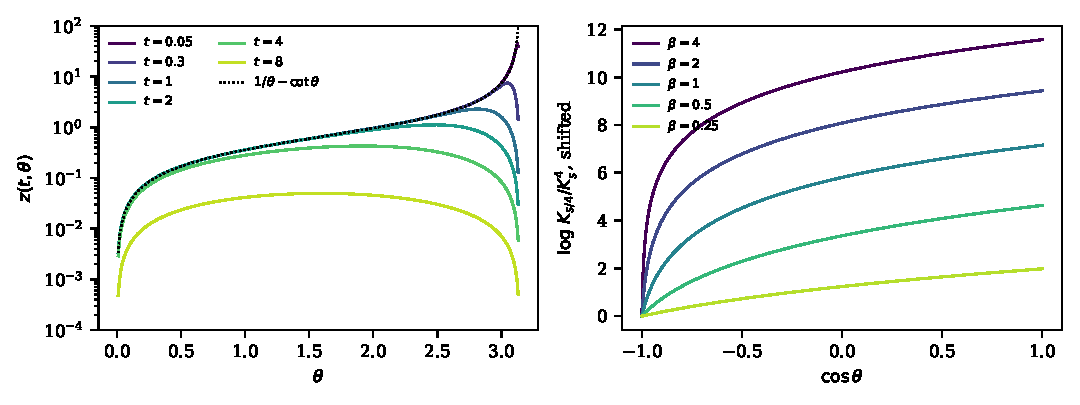
\includegraphics[width=\textwidth]{figures/contract.pdf}
\caption[The ladder contracts]{Left: $z(t,\theta)=\partial_t\big(t\,\partial_\theta\log K_t\big)$ at six times, on a logarithmic scale, with its small time limit $1/\theta-\cot\theta$; it is positive throughout, which is Theorem~\ref{thm:scaledmlr}. Right: the logarithm of the likelihood ratio $K_{t/4}/K_t^4$ against $\cos\theta$ at five couplings $\beta=2/t$, shifted to vanish at the antipode; it is increasing, which is Corollary~\ref{cor:contracts}.}
\label{fig:contract}
\end{figure}

The initial layer uses two formulas. The first is the method of images: up to a factor depending on $t$ alone,
\[
K_t\sin\theta=H(\theta,t)=\sum_{j\in\mathbb Z}\theta_j\,e^{-\theta_j^2/t},\qquad\theta_j=\theta+2\pi j,
\]
so that $z=\partial_t\big(tH'/H\big)-\cot\theta$.
The second is the product formula. The Jacobi triple product behind Theorem~\ref{thm:product} gives $K_t=\frac12\vartheta\,S_1$ with $\vartheta\propto\prod_n(1+x/C_n)$ and $S_1=\partial_x\log\vartheta=\sum_n1/(C_n+x)$. So, with $a_n=1/(C_n+x)$, $S_p=\sum a_n^p$ and $B_p=\sum C_n'a_n^p$,
\[
G=S_1-\frac{S_2}{S_1},\qquad\zeta=-\partial_t(tG)=t\Big(B_2-\frac{2B_3}{S_1}+\frac{B_2S_2}{S_1^2}\Big)-S_1+\frac{S_2}{S_1},
\]
and $z=\zeta\sin\theta$.

\begin{lemma}[perturbation]\label{lem:perturb}
Let $H=H_0(1+E)$ and let $z_0$ be defined from $H_0$ as $z$ is from $H$. If $t\le1$ and $|E|$, $|E'|$, $|\partial_tE|$, $|\partial_tE'|$ are at most $\delta\le\frac12$ at a point, then $|z-z_0|\le6\delta$ there. If moreover $|E'|$ and $|\partial_tE'|$ are at most $\theta\delta$, then $|z-z_0|\le6\theta\delta$.
\end{lemma}

\begin{proof}
$tH'/H=tH_0'/H_0+tE'/(1+E)$, and $\partial_t\big[tE'/(1+E)\big]=E'/(1+E)+t\,\partial_tE'/(1+E)-tE'\partial_tE/(1+E)^2$.
\end{proof}

\begin{proposition}[the initial layer]\label{prop:initial}
For $0<t\le0.1$ and $0<\theta<\pi$, $z(t,\theta)>0$.
\end{proposition}

\begin{proof}
Write $\epsilon=\pi-\theta$ and $u=2\pi\epsilon/t$. Three regions cover $(0,\pi)$.

\emph{Near the identity, $\theta\le\pi/2$.} Take $H_0=\theta e^{-\theta^2/t}$, for which $z_0=1/\theta-\cot\theta\ge\theta/3$. Pairing the images $j$ and $-j$,
\[
E=\sum_{j\ge1}e^{-4\pi^2j^2/t}\Big[2\cosh(\omega_j\theta)-t\omega_j^2\,\frac{\sinh(\omega_j\theta)}{\omega_j\theta}\Big],\qquad \omega_j=\frac{4\pi j}{t},
\]
an even entire function of $\theta$. Every derivative of $\sinh w/w=\int_0^1\cosh(ws)\,ds$ is bounded by $\cosh w$, so a derivative in $\theta$ costs a factor $\omega_j$ and a derivative in $t$ a factor at most $4\pi^2j^2/t^2+\omega_j\theta/t+2/t$, with an extra $\omega_j^2$ from the coefficient $t\omega_j^2$. With $\omega_j\theta\le2\pi^2j/t$ the exponentials combine to at most $e^{-2\pi^2j^2/t}$, and for $t\le0.1$ the term $j=1$ of each of $E$, $\partial_tE$, $E''$, $\partial_tE''$ is at most $1.6\times10^6\,t^{-5}e^{-2\pi^2/t}$, the remaining terms adding less than as much again. Since $t^{-5}e^{-2\pi^2/t}$ increases on $(0,0.1]$, all four are below $\delta=10^{-74}$. Because $E$ is even, $|E'|$ and $|\partial_tE'|$ are at most $\theta\delta$, and Lemma~\ref{lem:perturb} gives $z\ge\theta/3-6\theta\delta>0$.

\emph{The middle, $t/4\le\epsilon\le\pi/2$.} Take for $H_0$ the images $j=0$ and $j=-1$:
\[
H_0=2e^{-(\pi^2+\epsilon^2)/t}\big(\pi\sinh u-\epsilon\cosh u\big),\qquad\frac{tH_0'}{H_0}=2\epsilon-\frac{2\pi^2-t-2\pi\epsilon\varrho}{\mathcal D},
\]
with $\varrho=\tanh u$ and $\mathcal D=\pi\varrho-\epsilon$, and therefore
\[
z_0=z_2=\cot\epsilon+\frac1{\mathcal D}-\frac1\epsilon\Big(\frac{u}{\sinh u}\Big)^2\Big(\frac{\pi\varrho}{\mathcal D}\Big)^2\Big(1-\frac{2\epsilon^2+t}{2\pi^2}\Big).
\]
Here $u\ge\pi/2$, so $\varrho\ge0.917$, $\mathcal D\ge1.31$ and $(u/\sinh u)^2\le0.466$. The last term is at most $\epsilon^{-1}(u/\sinh u)^2(\pi\varrho/\mathcal D)^2$, which at fixed $\epsilon$ decreases as $t$ decreases, because $u$ grows; so it is enough to bound it at $t=0.1$, where $u=20\pi\epsilon$. For $\epsilon\le0.05$: $(\pi\varrho/\mathcal D)^2\le1.036$ and, with $\cot\epsilon\ge1/\epsilon-\epsilon/2$, $z_2\ge0.517/\epsilon-\epsilon/2\ge10$. For $0.05\le\epsilon\le0.1$: $u\ge\pi$, $(u/\sinh u)^2\le0.074$, $(\pi\varrho/\mathcal D)^2\le1.07$, and $z_2\ge0.92/\epsilon-0.05\ge9$. For $\epsilon\ge0.1$: $u\ge2\pi$, $(u/\sinh u)^2\le6\times10^{-4}$, $(\pi\varrho/\mathcal D)^2\le4.84$, the last term is below $0.03$, and $z_2\ge\cot\epsilon+1/\mathcal D-0.03\ge1/\pi-0.03>0.28$.

For the error, $H_0\ge1.31\,e^{-\theta^2/t}\ge1.31\,e^{-\pi^2/t}$, while the remaining images are at distance at least $5\pi/2$ from the origin, so they and their first derivatives in $\theta$ and $t$ are at most $1.6\times10^4\,t^{-3}e^{-25\pi^2/(4t)}$. From the formulas above, $|H_0'/H_0|\le19/t$, $|\partial_tH_0/H_0|\le49/t^2$ and $|\partial_t(H_0'/H_0)|\le360/t^3$. Hence $E$, $E'$, $\partial_tE$ and $\partial_tE'$ are at most $1.6\times10^7\,t^{-6}e^{-51.8/t}<10^{-200}$ for $t\le0.1$, and Lemma~\ref{lem:perturb} gives $z\ge0.28-10^{-199}>0$.

\emph{The cap, $\epsilon\le t/4$.} Here no asymptotics are needed, and the argument holds for every $t>0$. By Euler's relation for the homogeneous function $G$ of the $a_j$, $\zeta=\sum_jw_ja_j\big(tC_j'a_j-1\big)$ with $w_j=(1-p_j)^2+\sum_{n\ne j}p_n^2\ge0$ and $p_n=a_n/S_1$. With $y_j=(2j-1)t/4$, $tC_j'a_j=y_j\sinh y_j/(\cosh y_j+x)$, which is at least one when $x\le \ell(y_j)=y_j\sinh y_j-\cosh y_j$. The function $\ell$ is increasing and $\ell(y)\ge-1+y^2/2$, while $x=-\cos\epsilon\le-1+\epsilon^2/2$. So for $\epsilon\le t/4=y_1$ every term is nonnegative and those with $j\ge2$ are positive.
\end{proof}

\paragraph{\normalfont\scshape Checks.} The proof uses no computation, but each part was checked by one (\texttt{initial\_layer.py} and \texttt{ladder\_certificate.py}). The model $z_2$ agrees with $z$ computed from thirteen images in sixty digit arithmetic to the precision of the numerical derivative, and its minimum on $[t/4,\pi/2]$ is $2/\pi$, at $\epsilon=\pi/2$, for $t=0.1$, $0.03$ and $0.002$; the three lower bounds of the proof hold on a grid of four hundred points at each. Independently of the proposition, positivity of $\zeta(t_0,\cdot)$ on $[-1,1]$ was checked by an enclosure at $t_0=2$, $0.5$, $0.1$, $0.02$, $0.005$ and $0.002$: each of the four sums in $\zeta$ has positive terms decreasing in $x$, so on a box it lies between its values at the endpoints, and bisection until the lower bound is positive covers the interval with $50$ to $7370$ boxes, with an allowance of $10^{-9}$ for rounding and tails and with the sums evaluated in the variable $1+x$ to avoid cancellation at the antipode.

\begin{corollary}[the ladder contracts]\label{cor:contracts}
Let $k>1$ and $t>0$. Then $K_{t/k}/K_t^k$ is strictly increasing in $\cos\theta$: the bond moved law is strictly above the heat kernel at time $t/k$ in the likelihood ratio order of the angle used in Proposition~\ref{prop:localtime}. Consequently
\[
\frac{\int\cos\theta\,K_t^k}{\int K_t^k}<e^{-3t/(4k)},
\]
and the heat kernel projected Migdal Kadanoff map with scale factor $b$ in dimension $d$, where $k=b^{d-2}$, sends the time $t$ to $t'>b^{4-d}t$. In four dimensions $R(\beta)<\beta$ for every $\beta>0$ and every $b$. In three dimensions $t'>bt$.
\end{corollary}

\begin{proof}
$\partial_x\big[\log K_{t/k}-k\log K_t\big]=G(t/k,x)-kG(t,x)=\frac kt\big[(t/k)G(t/k,x)-tG(t,x)\big]>0$ by the theorem, since $t/k<t$. Likelihood ratio order implies the order of the means of $\cos\theta$, and the mean under $K_{t/k}$ is $u_2(t/k)=e^{-3t/(4k)}$. Decimation raises the fundamental coefficient to the power $b^2$, so $u_2'<e^{-3b^2t/(4k)}$ and $t'=-\frac43\log u_2'>b^2t/k$.
\end{proof}

Four remarks.

First, this settles the first problem of Chapter~\ref{ch:programme}: the projected ladder of SU(2) moves every coupling strictly toward strong coupling at every rung, for every scale factor. Nothing in four dimensions changes; this is a theorem about the heat kernel projection of the hierarchical model. For the exact ladder the bond moving half is the same statement, and the decimation half needs convolution to preserve the order, which is the problem of the bad cap above.

Second, the proof rests on two supports: a theorem from geometric analysis, Hamilton's inequality, used through the maximum principle; and an explicit small time estimate from the method of images, with margins of seventy orders of magnitude and more. It is not computer assisted. An enclosure at fixed time slices serves as an independent check, described above.

Third, the proof explains the direction of the flow. The decrement of the ladder is the amount by which $t\,\partial_x\log K_t$ falls between $t/k$ and $t$, and it is positive because of Hamilton's inequality, which is a statement of nonnegative curvature. In flat space there is equality and no running; on a group there is curvature and the coupling runs to strong coupling. Hamilton's inequality holds on every compact Lie group with its biinvariant metric, so the Hamilton part of Step 2 is available for SU(N), although the sign of $-v$ came from the SU(2) product formula; Steps 1 and 3 used one angle and need the Weyl chamber in general.

Fourth, the theorem has a short proof of the likelihood ratio property as a byproduct. $G=2\sum_{m<n}a_ma_n/\sum_na_n$ has $\partial G/\partial a_j=(1-p_j)^2+\sum_{n\ne j}p_n^2\ge0$ with $p_n=a_n/S_1$, and each $a_j$ decreases in $t$; so $G$ decreases in $t$, which is Corollary~\ref{cor:mlrall}.

\section{The string tension on the hierarchical lattice exists}

\begin{proposition}\label{prop:sigmaexists}
Let $u^{(m)}_2$ be the second character coefficient after $m$ steps of the ladder with bond moving power $k$ and decimation power $b^2$. If $u_2^{(m)}\to0$ and $0\le u_n^{(m)}\le(u_2^{(m)})^{n-1}$ for every $n\ge2$ and every $m$, then
\[
\sigma a^2=\lim_{m\to\infty}b^{-2m}\big(-\log u_2^{(m)}\big)
\]
exists, the convergence is geometric, and the limit is positive.
\end{proposition}

\begin{proof}
Write $v_m=-\log u_2^{(m)}$. When $u_2$ is small all higher coefficients are smaller, the law is $1+2u_2\chi_2+\cdots$ times Haar measure, and bond moving gives a second coefficient $k\,u_2(1+O(u_2))$. Decimation raises it to the power $b^2$. Hence $v_{m+1}=b^2\big(v_m-\log k+O(e^{-v_m})\big)$, and
\[
b^{-2(m+1)}v_{m+1}-b^{-2m}v_m=b^{-2m}\big(-\log k+O(e^{-v_m})\big).
\]
The increments are bounded by a geometric series, so the limit exists. Summing them from a rung $m_0$ onward, the limit is at least $b^{-2m_0}\big(v_{m_0}-\frac{b^2}{b^2-1}\log k-\varepsilon\big)$, with $\varepsilon>0$ the accumulated $O(e^{-v_m})$ terms, which can be made as small as we like by taking $m_0$ large, and which is positive as soon as $v_{m_0}$ exceeds $\frac{b^2}{b^2-1}\log k$; and $v_m\to\infty$ by hypothesis.
\end{proof}

For $b=2$ in four dimensions the threshold is $u_2<4^{-4/3}=0.157$. The hypothesis $u_2^{(m)}\to0$ is the statement that the flow reaches strong coupling, which for the projected ladder follows from Corollary~\ref{cor:contracts} and the continuity of $R$, and for the exact ladder is checked only numerically. The proposition makes precise the sense in which the ladder confines: once the flow enters the strong coupling region the string tension is fixed, up to the factor $b^{-2m}$ that counts how many rungs it took to get there. Asymptotic freedom is then the statement that the number of rungs grows linearly in $\beta$, with slope given by Theorem~\ref{thm:expansion}.

\section{The absolute string tension from the ladder}

By Proposition~\ref{prop:sigmaexists} the ladder predicts the string tension in lattice units, with no fitted constant. Under one step lengths scale by $b$ and areas by $b^2$, so
\[
\sigma a^2(\beta)=\lim_{m\to\infty}b^{-2m}\big(-\log u_2^{(m)}\big),
\]
where $u_2^{(m)}$ is the second character coefficient after $m$ steps from the Wilson law at $\beta$; the limit is reached geometrically once the flow is at strong coupling. We computed it for SU(2) in four and three dimensions (Figure~\ref{fig:mksigma}).

\begin{figure}[t]
\centering
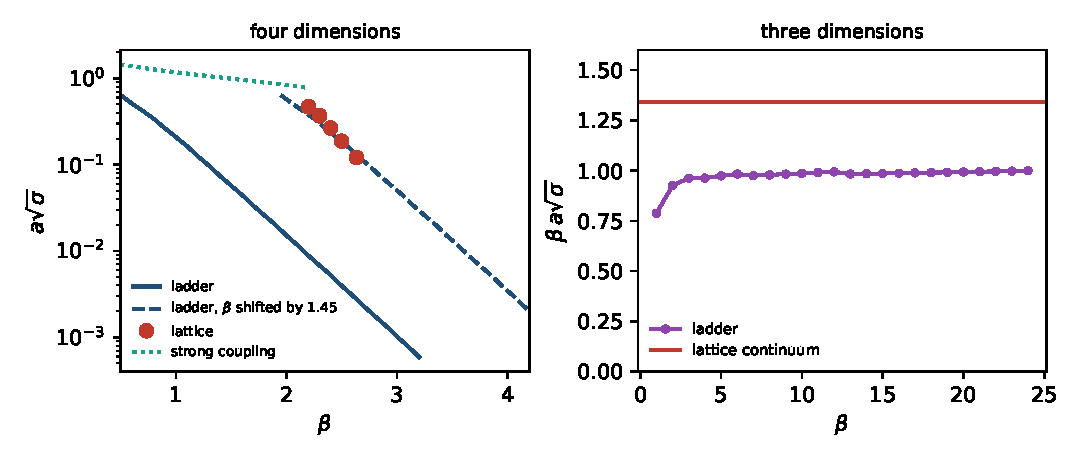
\includegraphics[width=\textwidth]{figures/mk_sigma.pdf}
\caption[Absolute string tension from the ladder]{Left: $a\sqrt\sigma$ in four dimensions from the ladder with Wilson start, the same curve shifted by $1.45$ in $\beta$, the lattice data, and the leading strong coupling formula. Right: $\beta a\sqrt\sigma$ in three dimensions from the ladder, against the continuum value $1.341$ of lattice simulations.}
\label{fig:mksigma}
\end{figure}

In four dimensions the ladder gives $a\sqrt\sigma=0.0088$, $0.0068$, $0.0053$, $0.0039$ and $0.0028$ at $\beta=2.2$, $2.3$, $2.4$, $2.5$ and $2.635$, against the lattice values $0.469$ to $0.121$: too small by a factor between $43$ and $54$ across the window. A constant factor in the lattice spacing is a shift of the coupling, here by about $1.45$: the ladder places the crossover to strong coupling near $\beta=0.8$, where the real theory has it near $\beta=2.2$. The cause is visible in the first step, where bond moving multiplies the bare coupling by $b^{d-2}=4$ before any decimation. In the language of perturbation theory the ladder has the rate of running right to ten or fifteen percent in the window and the wrong $\Lambda$ parameter by a factor of fifty.

In three dimensions the coupling has dimensions of mass and $a\sqrt\sigma$ is proportional to $1/\beta$ at weak coupling. Lattice simulations~\cite{Te99} give $\sqrt\sigma/g^2=0.3353$, that is $\beta a\sqrt\sigma=1.341$ in the continuum limit. The ladder gives values between $0.98$ and $1.00$ for $8\le\beta\le32$, with mean $0.99$, with a modulation of about two percent in $\log_2\beta$ left by the discrete scale factor. It is low by a quarter: far better than in four dimensions, because in three dimensions the scale is set by the coupling itself and not by an exponentially sensitive crossover.

\begin{quote}
\textsc{Status.} The ladder is a qualitative caricature with quantitative errors of known size: ten to fifteen percent in the rate of running, a factor of two in the two loop coefficient, a shift of $1.45$ in the four dimensional coupling, and twenty six percent in the three dimensional string tension. A comparison theorem for step 4 need not be tight, since any pair of brackets with positive decrement gives a gap. But these numbers say how far apart the brackets must be allowed to lie, and they recommend three dimensions as the place to try first; Chapter~\ref{ch:sandwich} and Section~\ref{ch:threed} take up both points.
\end{quote}

\section*{Exercises}
\begin{enumerate}
\item In Proposition~\ref{thm:mlrlarge}, prove the bound $|U_{n-1}'(x)|\le(n^3-n)/3$ on $[-1,1]$ from the identity $U_{n-1}'(1)=(n^3-n)/3$ and the fact that a Gegenbauer polynomial of positive index attains its largest modulus on $[-1,1]$ at $x=1$.
\item Show that the mixed partial of $\log(\theta e^{-\theta^2/t})$ in $t$ and $\theta$ is $2\theta/t^2$, and relate it to the small time limit of Corollary~\ref{cor:mlrall}.
\item Show that the critical points of a polynomial with real zeros are nondecreasing functions of each zero.
\item Verify Proposition~\ref{prop:wilsonflow} at $\kappa=3/2$ by expanding near $\theta=\pi$.
\item Derive the two loop decrement $\delta_{\mathrm{pert}}$ from the two loop beta function and show that its $1/\beta$ coefficient is invariant under $\beta\mapsto\beta+c$.
\item Repeat the scaling test of this chapter for SU(3) with $b=2$, using Theorem~\ref{thm:expansionN}, where the ladder predicts $d\log a/d\beta=-\log2\cdot16/9$ in units where $\beta=6/g^2$.
\end{enumerate}

\chapter{Inequalities Between the Ladder and the Lattice}\label{ch:sandwich}\index{sandwich}\index{Wilson loop}\index{likelihood ratio order}\index{propagation of chaos}\index{perturbation theory!lattice}\index{Monte Carlo renormalization group}

Chapter~\ref{ch:progress} reported what has been proved and what has been measured on the open problems of the path. This chapter closes Part V with the comparison that the path needs most, between the ladder and the lattice. Step 4 of the path asks for two caricatures whose flows bracket the true block spin flow. The first half of the chapter tests the idea in the one case where the truth can be measured cheaply: a single step of scale factor two, in four dimensions, on the law of one blocked plaquette. At every coupling we tried, the measured law lies between the two caricatures in mean, and in the likelihood ratio order on most of its mass. The second half, Section~\ref{ch:griffiths}, recalls the correlation inequalities that are known, shows that the independent end of the bracket is a theorem for expectations, and states what a proof of the other end would need.

\section{One step, three laws}

Block the lattice by decimation: the blocked link is the product of two consecutive links. The blocked plaquette is then the holonomy of a $2\times2$ Wilson loop, and its law, as a class function on SU(2), is a law on the rotation angle $\theta\in[0,\pi]$. Three laws of that angle can be compared.
\begin{itemize}
\item Measured. The law of the $2\times2$ holonomy in a simulation of the four dimensional theory.
\item Independent. The law the holonomy would have if the four plaquettes tiling the loop were independent: character coefficients $u_n^4$, with $u_n$ those of the measured single plaquette law. This is decimation without bond moving, and it is exact in two dimensions.
\item Migdal Kadanoff \cite{Mi75,Ka76}. Bond moving with power $b^{d-2}=4$ applied to the measured plaquette law, then decimation.
\end{itemize}
The second ignores the plaquettes off the plane of the loop. The third counts them at full strength, as if each were an independent copy acting on the same variable. The truth should lie between.

\section{The measurement}

We ran the heat bath of Section~\ref{ch:latticemc} on an $8^4$ lattice at six couplings, eighty sweeps of equilibration and sixty measurements four sweeps apart, recording histograms of the angle of every plaquette and every $2\times2$ loop. The table gives the mean $u_2=\E\cos\theta$ of the three laws.

\begin{center}
\small
\begin{tabular}{ccccc}
\toprule
$\beta$ & independent & measured & Migdal Kadanoff & $\log W_{22}/\log W_{11}$ \\ \midrule
2.2 & 0.106 & 0.137 & 0.589 & 3.54 \\
2.5 & 0.182 & 0.261 & 0.665 & 3.15 \\
3 & 0.274 & 0.380 & 0.733 & 2.99 \\
4 & 0.409 & 0.524 & 0.804 & 2.89 \\
6 & 0.573 & 0.675 & 0.875 & 2.82 \\
10 & 0.727 & 0.801 & 0.927 & 2.78 \\
\bottomrule
\end{tabular}
\end{center}

\begin{figure}[t]
\centering
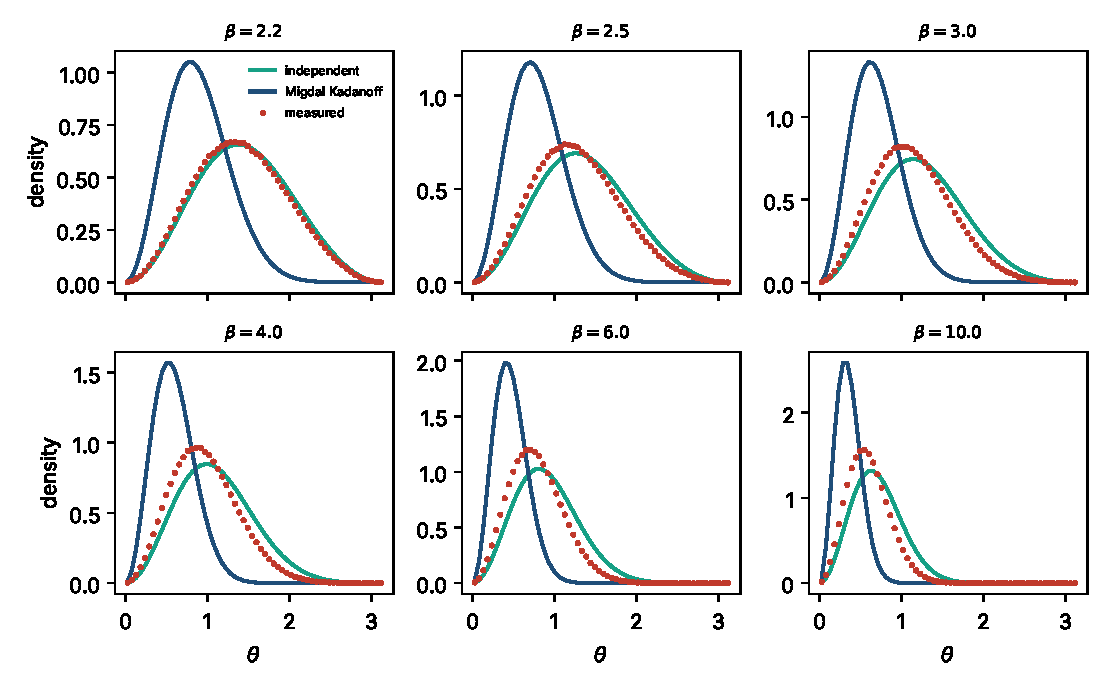
\includegraphics[width=\textwidth]{figures/sandwich.pdf}
\caption[An empirical sandwich for the blocked plaquette]{The law of the rotation angle of the $2\times2$ loop holonomy in four dimensional SU(2), measured on an $8^4$ lattice, between the law for independent plaquettes and the Migdal Kadanoff law, both built from the measured single plaquette law, at six couplings.}
\label{fig:sandwich}
\end{figure}

At every coupling the measured value lies strictly between the other two (Figure~\ref{fig:sandwich}). The last column is the ratio of the logarithms of the $2\times2$ loop and the plaquette. Independent plaquettes would give $4$; the Gaussian ledger of the ladder gives $1$; the simulation gives $3.5$ at the crossover, falling to $2.8$ at weak coupling (here $\beta$ up to $10$).

\section{The likelihood ratio order}

Beyond the means, the sandwich holds in the likelihood ratio order on most of the mass. We computed the two density ratios, independent over measured and measured over Migdal Kadanoff, on the sixty bins of the histograms. If each is increasing in $\theta$, then
\[
\text{Migdal Kadanoff}\ \le_{\mathrm{lr}}\ \text{measured}\ \le_{\mathrm{lr}}\ \text{independent}
\]
in the likelihood ratio order on the angle, to the extent that the ratios are increasing. Weighting bins by the measured mass, the ratio of measured to Migdal Kadanoff is increasing on all of the mass at every coupling. The ratio of independent to measured is increasing on all of the mass for $\beta\ge4$, on $97$ percent at $\beta=2.5$ and $3$, and on $84$ percent at $\beta=2.2$, where the two laws are close and the histogram noise is comparable to their difference. The order is therefore a measured property of most of the mass, not of every bin, and we do not claim it for whole laws.

This is the order in which Chapter~\ref{ch:path} proposed to state the comparison, because bond moving preserves it, and convolution preserves it under the condition of Theorem~\ref{thm:tp2}, which bond moved heat kernel laws satisfy on the near hemisphere $(0,\pi/2]$ (Theorem~\ref{thm:hemisphere}) and, to leading order and numerically, away from a cap at the antipode.

\section{How independent are plaquettes?}

The Migdal Kadanoff approximation and the independent caricature both treat plaquettes at one scale as independent. We measured the correlation of $\frac12\operatorname{tr}U_p$ between neighbouring plaquettes in the same runs.

\begin{center}
\small
\begin{tabular}{cp{1.1in}p{1.1in}p{1.1in}}
\toprule
$\beta$ & same plane, sharing a link & parallel, one step apart & orthogonal planes, sharing a link \\ \midrule
2.2 & 0.010 & 0.035 & 0.043 \\
2.5 & 0.013 & 0.027 & 0.045 \\
4 & 0.017 & 0.021 & 0.046 \\
10 & 0.018 & 0.021 & 0.046 \\
\bottomrule
\end{tabular}
\end{center}

Every correlation is below five percent, at every coupling. Plaquettes are pairwise almost independent, in a loose sense of propagation of chaos, and yet the $2\times2$ loop is far from the product of four independent plaquettes: its logarithm is $2.8$ to $3.5$ times that of a plaquette and not $4$ times. Weak pairwise correlations of one sign, summed coherently over the many plaquettes that touch the loop, produce an effect of order one. That is the content of bond moving, and it explains why the independent caricature fails although pairwise independence nearly holds.

\section{Two steps, and three dimensions}

The same test can be iterated and moved to three dimensions. We measured the laws of the plaquette, the $2\times2$ loop and the $4\times4$ loop, on an $8^4$ lattice at four couplings and on a $16^3$ lattice at four couplings, with a hundred sweeps of equilibration and eighty measurements. In four dimensions the $4\times4$ loop spans half of the periodic box, which limits what these data can show (see below). In three dimensions bond moving has power $b^{d-2}=2$. For each ensemble there are three comparisons: one step from the plaquette to the $2\times2$ loop; one step from the measured $2\times2$ law to the $4\times4$ loop; and two steps from the plaquette to the $4\times4$ loop, with each caricature applied twice. To place the truth inside the bracket we use
\[
\xi=\frac{\log u_2^{\mathrm{meas}}-\log u_2^{\mathrm{ind}}}{\log u_2^{\mathrm{MK}}-\log u_2^{\mathrm{ind}}},
\]
which is $0$ for independent plaquettes and $1$ for Migdal Kadanoff.

\begin{center}
\footnotesize
\begin{tabular}{cccccccc}
\toprule
 & & \multicolumn{3}{c}{$u_2$ of the $4\times4$ loop, two steps} & \multicolumn{3}{c}{position $\xi$} \\
$d$ & $\beta$ & indep. & measured & MK & 1 to 2 & 2 to 4 & 1 to 4 \\ \midrule
4 & 2.5 & 0.0011 & 0.026 & 0.648 & 0.28 & 0.48 & 0.49 \\
4 & 3 & 0.0057 & 0.086 & 0.721 & 0.33 & 0.52 & 0.56 \\
4 & 4 & 0.028 & 0.202 & 0.799 & 0.37 & 0.53 & 0.59 \\
4 & 6 & 0.108 & 0.388 & 0.874 & 0.39 & 0.54 & 0.61 \\
3 & 4 & 0.0062 & 0.021 & 0.267 & 0.22 & 0.33 & 0.32 \\
3 & 6 & 0.046 & 0.126 & 0.456 & 0.31 & 0.44 & 0.44 \\
3 & 9 & 0.143 & 0.305 & 0.613 & 0.36 & 0.53 & 0.52 \\
3 & 14 & 0.298 & 0.494 & 0.740 & 0.39 & 0.56 & 0.56 \\
\bottomrule
\end{tabular}
\end{center}

\begin{figure}[t]
\centering
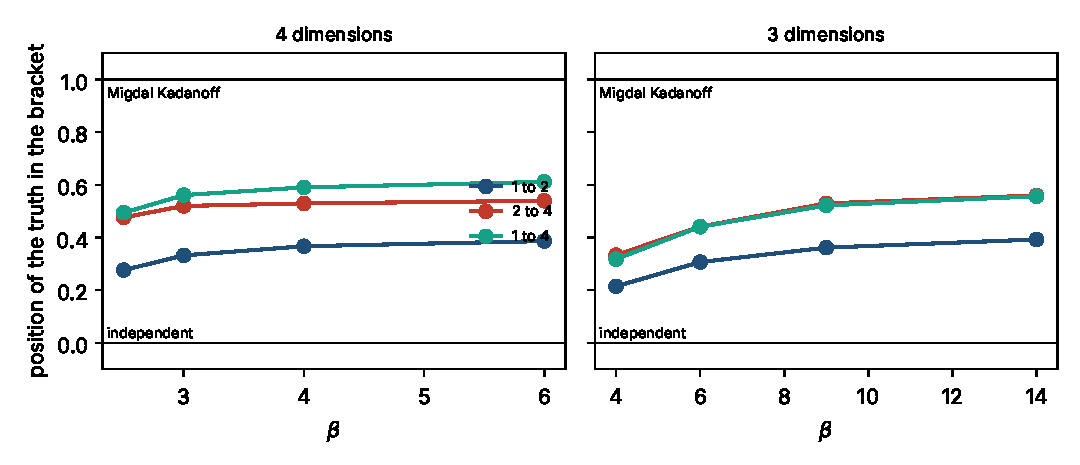
\includegraphics[width=\textwidth]{figures/sandwich2.pdf}
\caption[Position of the truth inside the bracket]{The position $\xi$ of the measured loop law between the independent caricature, $\xi=0$, and the Migdal Kadanoff caricature, $\xi=1$, for one step from the plaquette, one step from the $2\times2$ loop, and two steps, in four and three dimensions.}
\label{fig:sandwich2}
\end{figure}

In all twenty four comparisons the truth lies inside the bracket (Figure~\ref{fig:sandwich2}). The bracket survives a second step: after two applications the caricatures are far apart, a factor of six hundred at $\beta=2.5$ in four dimensions, and the truth sits near the middle on a logarithmic scale. The position drifts upward with the scale, from about $0.35$ at the first step to about $0.55$ at the second, and upward with $\beta$. We read this as a trend in these data only. In four dimensions the $4\times4$ loops live on a periodic $8^4$ lattice, where the loop spans half the box and the runs at $\beta\ge3$ lie above the deconfinement coupling $\beta_c=2.51$ of temporal extent $8$ (Section~\ref{ch:missing}), so finite size effects on these loops are not controlled. Whether the truth moves toward Migdal Kadanoff at larger scales and weaker coupling, as it must if the ladder is to be right about the marginal flow, needs larger lattices. The likelihood ratio order holds on at least $95$ percent of the mass in eighteen of the twenty four comparisons; the exceptions are at the strongest couplings in each dimension, mostly $4\times4$ loops whose laws are within noise of Haar measure.

In three dimensions the bracket is narrower, as Section~\ref{ch:threed} anticipated: at the first step the two caricatures differ by a factor of $1.2$ to $1.9$ in $u_2$, against $1.5$ to $3.7$ in four dimensions.

\section{The sandwich at weak coupling, to leading order}

At weak coupling the three laws can be compared analytically. To lowest order in lattice perturbation theory, in $d$ dimensions,
\[
-\log W_{RR}=\frac{g^2C_F}{2}\int\frac{\mathrm d^dk}{(2\pi)^d}\,F_R(k_\mu)F_R(k_\nu)\,\frac{\hat k_\mu^2+\hat k_\nu^2}{\hat k^2},
\]
where $C_F$ is the quadratic Casimir of the representation, $F_R(k)=\sin^2(kR/2)/\sin^2(k/2)$ and
$\hat k_\rho=2\sin(k_\rho/2)$: the form factor of the $R\times R$ surface against the propagator of the field strength. For $R=1$ the integral is $2/d$, which gives the plaquette $1-3/(4\beta)$ of SU(2) in four dimensions. The ratio $\kappa_R=\log W_{RR}/\log W_{11}$ is then a pure number, the same for every gauge group. We evaluated the momentum sums numerically, in floating point, on lattices up to $32^4$ and $128^3$, with no error bound; the entries below are numerical results for a leading order formula, not theorems.

\begin{center}
\small
\begin{tabular}{cccccc}
\toprule
$d$ & loop & indep. & perturbation theory & MK & position $\xi$ \\ \midrule
4 & $2\times2$ & 4 & 2.739 & 1 & 0.42 \\
4 & $4\times4$ & 16 & 6.523 & 1 & 0.63 \\
3 & $2\times2$ & 4 & 3.120 & 2 & 0.44 \\
3 & $4\times4$ & 16 & 8.715 & 4 & 0.61 \\
\bottomrule
\end{tabular}
\end{center}

The four rows of the table suggest the following statement, which we do not prove.

\begin{conjecture}\label{prop:weaksandwich}
To leading order at weak coupling, in three and four dimensions and for every gauge group, the logarithm of the $2\times2$ and $4\times4$ Wilson loops lies strictly between the values given by independent plaquettes and by the Gaussian ledger of the Migdal Kadanoff ladder.
\end{conjecture}

A proof would need explicit bounds on the infinite volume integrals above.

The simulations approach these limits as they should. In four dimensions the measured ratio $\log W_{22}/\log W_{11}$ is $2.82$ at $\beta=6$ and $2.78$ at $\beta=10$, against $2.735$ for the same sum on an $8^4$ lattice; in three dimensions it is $3.21$ at $\beta=14$ against $3.12$. The measured positions, $0.39$ and $0.61$ in four dimensions at $\beta=6$, are approaching $0.42$ and $0.63$. This also validates the heat bath code against an independent calculation.

At strong coupling the comparison is with the other end of the bracket. A leading order cluster expansion argument, not a proof, gives $W_{22}=W_{11}^4$ to the first orders in $u_2$, because the leading corrections to each side are the same sixteen elementary cubes attached to the same four plaquettes, so the truth approaches the independent caricature, $\xi\to0$, as the data show. The truth therefore travels across the bracket as the coupling weakens, from the independent end toward a limiting position near the middle, and never leaves it in our data. The open part of the problem below is the crossover region, where neither expansion applies.

\section{What the sandwich does and does not show}

It shows that at one step the two caricatures bracket the truth in the right order, at weak coupling, at the crossover and in between. It also locates the truth inside the bracket: in the Gaussian ledger, a bond moving power $k$ gives the ratio $4/k$ in the last column of the first table, so the measured ratios correspond to an effective power between $1.13$ at $\beta=2.2$ and $1.44$ at $\beta=10$, against the ladder's $4$. The ladder overcounts the off plane plaquettes by a factor of about three in this measure, which is the single step form of its misplaced crossover.

It shows the bracket surviving one iteration, at the level of loop laws. It does not show that it survives the iteration that matters, of the effective action. The law of a Wilson loop is not the plaquette law of the blocked effective action: decimation generates couplings of all shapes, and the perimeter self energy of the loop lowers its expectation without lowering the effective coupling. A faithful test iterates a block transformation that keeps the action nearly local, such as the smeared blockings used in Monte Carlo renormalization \cite{Sw79}, fits the plaquette law of each blocked ensemble by the pseudolikelihood of Section~\ref{ch:slice}, and compares rung by rung. The particle ladder of Section~\ref{ch:h6} is the tool for running the two caricatures alongside.

\section{A first empirical rung}

The faithful test described above can be started with the tools already built. We blocked $8^4$ configurations to $4^4$ by two rules, plain decimation, and decimation with the $2\times1$ staples added with weight one half and the sum projected back to SU(2), and fitted a single plaquette Wilson coupling to each ensemble by the pseudolikelihood of Section~\ref{ch:slice}, now with the six staples of four dimensions.

\begin{center}
\small
\begin{tabular}{ccccc}
\toprule
$\beta$ & unblocked & blocked, plain & blocked, smeared & ladder $R(\beta)$ \\ \midrule
2.2 & 2.201 & 0.52 & 1.85 & 1.94 \\
2.5 & 2.499 & 0.87 & 2.81 & 2.24 \\
3 & 3.006 & 1.14 & 4.03 & 2.74 \\
4 & 3.992 & 1.55 & 6.37 & 3.74 \\
6 & 6.010 & 2.26 & 11.2 & 5.75 \\
10 & 9.996 & 3.63 & 20.6 & 9.75 \\
\bottomrule
\end{tabular}
\end{center}

The second column is a validation: on the unblocked ensembles pseudolikelihood recovers the simulated coupling to two parts in a thousand. The next two columns are a caution. The coupling fitted to the blocked field depends strongly on the blocking rule: plain decimation gives about $0.36\beta$ from $\beta=2.5$ upward ($0.24\beta$ at $2.2$), far below the fine coupling, and smearing with weight one half gives up to about $2\beta$, above it from $\beta=2.5$ upward. The ladder's prediction lies between them at every coupling from $\beta=2.5$ upward, and so does the value $\beta-0.26$ that asymptotic freedom requires of a blocking that preserves the long distance physics.

Two lessons follow. A single fitted coupling is not a scheme independent description of the blocked theory; a faithful empirical ladder must fit a richer family of plaquette laws, with the character coefficients of Section~\ref{ch:latent} as parameters, or match observables between a blocked large lattice and an unblocked small one, as in Swendsen's Monte Carlo renormalization group \cite{Sw79}. And the blocking rule is itself a dial that moves the blocked law across the bracket, from the independent end at plain decimation toward and past the Migdal Kadanoff end as the smearing grows. Somewhere on that dial there may be a rule whose fitted coupling follows the renormalized trajectory, and the comparison problem can be posed for that rule. Section~\ref{ch:plgbc} selects a candidate rule at a few couplings on $8^4$ lattices, by matching with a trained generator in place of a fitted coupling; it does not show that the rule follows the trajectory.

\section{The independent end is a theorem}

At the level of means the independent end of the sandwich says $W_{22}\ge W_{11}^4$. For $\Z_2$ gauge theory this is Griffiths' second inequality \cite{Gri67}, in the many spin form of Ginibre \cite{Gi70}. For every compact group it follows from reflection positivity: Corollary~\ref{cor:griffiths} of Section~\ref{ch:griffiths} proves $W_{22}\ge W_{12}^2\ge W_{11}^4$ for every character, at every coupling and in every dimension. So the left ends of the brackets in the tables of this chapter are rigorous lower bounds, and the independent caricature is a true lower caricature for expectations. Theorem~\ref{thm:heatbath} of Section~\ref{ch:griffiths} gives a rigorous upper bound of the same form, with bond moving power $2(d-1)$, but acting on the Wilson weight and not on the measured plaquette law. The two rigorous ends therefore act on different laws: the lower on the measured plaquette law, the upper on the Wilson weight. The ladder's power $2^{d-2}$ lies between the two powers, but this is a comparison of powers and not a bracket of one quantity. Indeed the Migdal Kadanoff value of this chapter, which acts on the measured law, exceeds the proved bound $u(2(d-1)\beta)^4$ in four dimensions at the couplings $\beta=2.5,3,4,6,10$ ($0.665,0.733,0.804,0.875,0.927$ against $0.661,0.710,0.775,0.845,0.904$).

\begin{problem}\label{op:ineq1}
Prove that in SU(2) lattice gauge theory with the Wilson action the law of the $2\times2$ loop holonomy dominates, in the likelihood ratio order, the Migdal Kadanoff law built from the plaquette law, and that both halves of the sandwich hold in the likelihood ratio order. The Migdal Kadanoff end would be a first rigorous comparison between the lattice theory and the ladder at intermediate coupling, for the measured law. At the level of means and at those five couplings, the numbers above already put the measured $2\times2$ mean below the Migdal Kadanoff mean, and the proved bound of Theorem~\ref{thm:heatbath} lies below it too, so the new content of a proof would be the likelihood ratio order and the bound at every coupling.
\end{problem}

\section{Correlation Inequalities}\label{ch:griffiths}\index{Griffiths inequality}\index{Ginibre, J.}\index{correlation inequalities}\index{chessboard estimate}

The independent end of the sandwich above is a correlation inequality. This section recalls the inequalities that are known, with proofs short enough to show where commutativity is used, tests the smallest nonabelian case numerically, and states what a proof for SU(2) would need.

\subsection{Griffiths and Ginibre}

For the Ising model with ferromagnetic couplings, Griffiths \cite{Gri67} proved in 1967 that products of spins have nonnegative expectations and are positively correlated:
\[
\langle\sigma_A\rangle\ge0,\qquad\langle\sigma_A\sigma_B\rangle\ge\langle\sigma_A\rangle\langle\sigma_B\rangle,
\]
where $\sigma_A=\prod_{i\in A}\sigma_i$. Ginibre \cite{Gi70} gave in 1970 a general framework that covers plane rotators and other abelian models.

\begin{theorem}[Ginibre]\label{thm:ginibre}
Let $G$ be a compact abelian group with Haar measure, and $Q$ a convex cone of real continuous functions on $G^n$ that is closed under products and such that for all $f_1,\dots,f_m\in Q$ and all signs,
\[
\int\!\!\int\prod_{i=1}^m\big(f_i(x)\pm f_i(y)\big)\,\mathrm dx\,\mathrm dy\ge0 .
\]
If $-H\in Q$, then under the Gibbs measure $e^{-H}\mathrm dx/Z$, every $f,g\in Q$ satisfy $\langle f\rangle\ge0$ and $\langle fg\rangle\ge\langle f\rangle\langle g\rangle$.
\end{theorem}

\begin{proof}
Duplicate the system, with independent copies $x$ and $y$. Then
\[
2Z^2\big(\langle fg\rangle-\langle f\rangle\langle g\rangle\big)=\int\!\!\int\big(f(x)-f(y)\big)\big(g(x)-g(y)\big)\,e^{-H(x)-H(y)}\,\mathrm dx\,\mathrm dy .
\]
Expand the exponential in powers of $-H(x)-H(y)$, which is of the form $h(x)+h(y)$ with $h\in Q$; since $Q$ is a cone closed under products, each power is a combination with nonnegative coefficients of products of factors $h_j(x)+h_j(y)$. Every term of the expansion is an integral of a product of factors $f_i(x)\pm f_i(y)$ with $f_i\in Q$, hence nonnegative. The same expansion applied to $2Z^2\langle f\rangle=\int\!\!\int\big(f(x)+f(y)\big)e^{-H(x)-H(y)}\,\mathrm dx\,\mathrm dy$ gives $\langle f\rangle\ge0$.
\end{proof}

For the group $\Z_2$ the cone is generated by the products $\sigma_A$; for U(1) by the functions $\cos(\sum_im_i\theta_i)$. The hypothesis of the theorem is checked in the rotated variables: for U(1),
\begin{align*}
\cos a+\cos b&=2\cos\frac{a+b}{2}\cos\frac{a-b}{2},\\
\cos a-\cos b&=2\sin\frac{a+b}{2}\sin\frac{b-a}{2},
\end{align*}
so in the variables $(\theta_i+\theta_i')/2$ and $(\theta_i-\theta_i')/2$ every factor splits into a function of the half sums times the same function of the half differences, up to a reflection that preserves Haar measure, and the double integral factors into a square. That step is where the group must be abelian: it uses the change of variables to sums and differences of the two copies, which is a homomorphism only for a commutative group.

\subsection{Gauge theories}

A lattice gauge theory with group $\Z_2$ or U(1) and Wilson action is of Ginibre's form: the action is a positive combination of plaquette characters, and Wilson loops are characters of products of link variables. Two consequences are classical and follow from Theorem~\ref{thm:ginibre}. Every Wilson loop is nondecreasing in every plaquette coupling. And, switching off all plaquettes outside the plane of a loop, the loop is bounded below by its value in the two dimensional theory, $W_{RT}\ge u^{RT}$ with $u$ the two dimensional plaquette, which bounds the string tension above.

The inequality of the sandwich is stronger: it compares the loop with a power of the plaquette of the same theory. For $\Z_2$, where the plaquette variable is a sign and the loop is literally the product of the four signs inside it, $W_{22}\ge W_{11}^4$ is Griffiths' second inequality applied three times. For U(1) the cosine of a sum of plaquette angles is not the product of the cosines, and we do not know whether the product form follows from Ginibre's theorem.

For nonabelian groups the duplicate variable argument has no analogue, since $(U,U')\mapsto(UU',UU'^{-1})$ does not preserve Haar measure in a useful way and characters of products do not factor; we know of no Ginibre theorem and no FKG inequality, the gap noted in Section~\ref{ch:latent} (the FKG inequality of Fortuin, Kasteleyn and Ginibre~\cite{FKG71}). The inequality of the sandwich nonetheless follows from reflection positivity, in three lines, for every compact gauge group.

\subsection{The inequality is a theorem}

Let $\Pi$ be a lattice hyperplane through sites, $r$ the reflection in it, and $\Theta F=\overline{F\circ r}$. For the Wilson action with $\beta\ge0$, Osterwalder and Seiler's reflection positivity \cite{OSe} holds for this reflection: $\langle F\,\Theta F\rangle\ge0$ for every function $F$ of the links in the closed half space on one side of $\Pi$, the links in $\Pi$ included. The form $(F,G)\mapsto\langle F\,\Theta G\rangle$ is therefore a positive semidefinite inner product and satisfies the Schwarz inequality.

\begin{theorem}[doubling inequality]\label{thm:doubling}
Let $G$ be a compact group, $\rho$ an irreducible unitary representation of dimension $d_\rho$, and $C$ a closed lattice path in the closed half space on one side of $\Pi$ that starts and ends at a site $x\in\Pi$. Let $C\#rC$ be the closed path that follows $C$ and then the reflection of $C$ backwards. Then, for the Wilson action at any $\beta\ge0$ and in any dimension,
\[
\Big|\frac{\langle\chi_\rho(U_C)\rangle}{d_\rho}\Big|^2\ \le\ \frac{\langle\chi_\rho(U_{C\#rC})\rangle}{d_\rho}.
\]
\end{theorem}

\begin{proof}
Let $F_{ab}=\rho(U_C)_{ab}$, a function of the links on one side. By gauge invariance at $x$, the matrix $\langle\rho(U_C)\rangle$ commutes with $\rho(g)$ for every $g$, so by Schur's lemma $\langle F_{ab}\rangle=\delta_{ab}\,\langle\chi_\rho(U_C)\rangle/d_\rho$. The Schwarz inequality with the constant function gives $|\langle F_{ab}\rangle|^2=|\langle F_{ab}\,\Theta1\rangle|^2\le\langle F_{ab}\,\Theta F_{ab}\rangle$. Summing over $a$ and $b$,
\begin{align*}
\frac{\langle\chi_\rho(U_C)\rangle^2}{d_\rho}&\le\Big\langle\sum_{a,b}\rho(U_C)_{ab}\,\overline{\rho(U_{rC})_{ab}}\Big\rangle\\
&=\big\langle\operatorname{tr}\rho\big(U_C\,U_{rC}^{-1}\big)\big\rangle=\langle\chi_\rho(U_{C\#rC})\rangle .
\end{align*}
\end{proof}

If $C$ runs along $\Pi$ for part of its length, that part cancels in $C\#rC$. Take $C$ a plaquette with one edge in $\Pi$: then $C\#rC$ is the $1\times2$ loop. Take $C$ the $1\times2$ loop with its long edge in $\Pi$: then $C\#rC$ is the $2\times2$ loop.

\begin{corollary}\label{cor:griffiths}
For every compact gauge group, every $\beta\ge0$, every dimension and every irreducible representation, with normalised characters,
\[
W_{12}\ge W_{11}^2,\qquad W_{22}\ge W_{12}^2\ge W_{11}^4,\qquad W_{2^p\times2^q}\ge W_{11}^{2^{p+q}} .
\]
In particular, along loops $2^p\times2^q$, the string tension satisfies $\sigma a^2\le-\log W_{11}$, and for SU(2) every character coefficient of the law of the $2\times2$ loop holonomy is at least that of the law built from four independent plaquettes: $u_n^{\mathrm{meas}}\ge(u_n^{\mathrm{plaq}})^4$ for all $n$.
\end{corollary}

The independent end of the sandwich is thus a theorem at the level of every character, at every coupling, including the crossover. It is a classical kind of statement, in the family of the loop inequalities derived from reflection positivity since the late 1970s, which also give the convexity of the static potential \cite{Ba86}. What the theorem does not give is the likelihood ratio order between the two laws, which is a statement about all characters jointly, and it says nothing about the Migdal Kadanoff end.

The proof also explains the numbers. The inequality is a Schwarz inequality between the plaquette and the constant function in the reflection positive inner product, so the deficit $W_{12}-W_{11}^2$ is the squared norm of the component of the plaquette orthogonal to the vacuum, transported across the plane: a sum over excited states $\sum_{E>0}|c_E|^2$ with the weights of the spectral measure of Chapter~\ref{ch:positivity}. It vanishes in two dimensions, where the link in $\Pi$ carries no excitations between the two plaquettes, and it is small at strong coupling, where correlations across the plane are weak.

\subsection{The smallest nonabelian test}

The simulations below were run before we had the theorem, as a test of a conjecture; they now serve as a check of the code and as a measurement of the deficit. The smallest case is two adjacent plaquettes, $W_{12}\ge W_{11}^2$. In two dimensions equality holds, because the plaquettes are independent. In four dimensions we measured both sides on an $8^4$ lattice, forty configurations five sweeps apart at each coupling.

\begin{center}
\small
\begin{tabular}{ccccc}
\toprule
$\beta$ & $W_{12}$ & $W_{11}^2$ & difference & standard error \\ \midrule
2.2 & 0.3424 & 0.3251 & 0.0173 & 0.0003 \\
2.5 & 0.4586 & 0.4265 & 0.0321 & 0.0002 \\
3 & 0.5602 & 0.5241 & 0.0362 & 0.0002 \\
4 & 0.6735 & 0.6392 & 0.0343 & 0.0002 \\
6 & 0.7841 & 0.7572 & 0.0269 & 0.0001 \\
10 & 0.8707 & 0.8526 & 0.0181 & 0.0001 \\
\bottomrule
\end{tabular}
\end{center}

The inequality holds at every coupling, by more than fifty standard errors. The difference is largest near $\beta=3$, just above the crossover, and vanishes at both ends: at strong coupling by the cluster property, and at weak coupling because both sides tend to one. In lowest order perturbation theory $\log W_{12}/\log W_{11}=1.724$ in four dimensions, less than two for the same reason that $\log W_{22}/\log W_{11}$ is less than four: the form factor of a larger surface suppresses the high momenta that dominate the plaquette. The resulting prediction, $W_{12}-W_{11}^2=e^{-2w}(e^{0.276w}-1)$ with $w=3/(4\beta)$, is positive at every coupling and describes the data from $\beta=4$ upward (Figure~\ref{fig:griffiths}).

\begin{figure}[t]
\centering
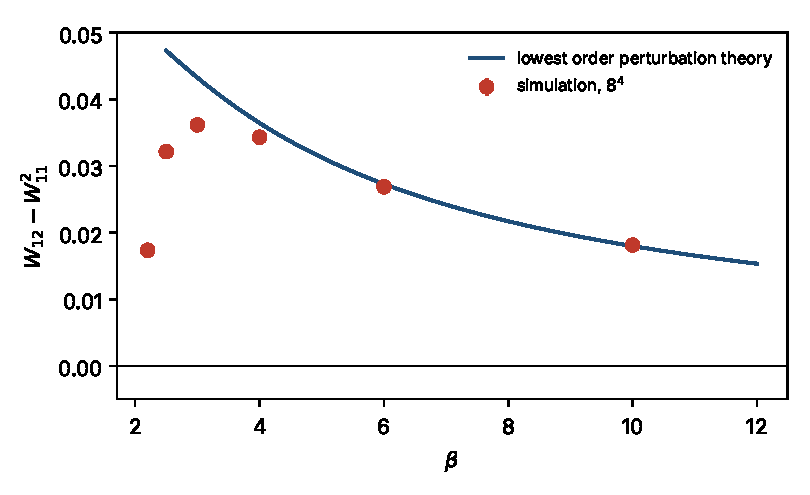
\includegraphics[width=0.8\textwidth]{figures/griffiths.pdf}
\caption[The smallest Griffiths test for SU(2)]{The difference $W_{12}-W_{11}^2$ for four dimensional SU(2) on an $8^4$ lattice, with bars of three standard errors, and the prediction of lowest order perturbation theory. The difference is positive at every coupling.}
\label{fig:griffiths}
\end{figure}

\subsection{The strong coupling side}

The table above stops at the crossover. Below it the difference is small and needs more statistics. We ran four hundred configurations at each of five strong couplings.

\begin{center}
\small
\begin{tabular}{cccc}
\toprule
$\beta$ & $W_{11}$ & $W_{12}-W_{11}^2$ & standard error \\ \midrule
1.2 & 0.290 & 0.00032 & 0.00010 \\
1.4 & 0.338 & 0.00042 & 0.00011 \\
1.6 & 0.388 & 0.00113 & 0.00009 \\
1.8 & 0.441 & 0.00327 & 0.00014 \\
2.0 & 0.501 & 0.00757 & 0.00009 \\
\bottomrule
\end{tabular}
\end{center}

The difference is positive at every coupling, by three standard errors at $\beta=1.2$ and by more than twelve from $\beta=1.6$ upward. It falls steeply, roughly like the eighth power of the plaquette, which is the order at which the strong coupling expansions of the two sides first differ: to order $u^6$ both are $u^2$ plus the same elementary cubes attached to the same two plaquettes, and at order $u^8$ the loop has surfaces spanning both plaquettes at once that the product does not. A naive count of those surfaces gives $2(d-2)u^8$; the data are about half of that between $\beta=1.4$ and $2$, so terms with higher representations contribute at the same order with the opposite sign, and we have not computed the coefficient. With the six couplings from the crossover upward, the inequality has been checked at eleven couplings from $\beta=1.2$ to $\beta=10$.

\subsection{A rigorous upper bound}

The other side has a classical answer too, of a different kind. Integrate out some of the links of the loop exactly.

\begin{theorem}[heat bath bound]\label{thm:heatbath}
Let $C$ be a closed lattice path without repeated links, and $A$ a set of links of $C$ no two of which lie in a common plaquette. For SU(2) with the Wilson action in $d$ dimensions, with $u(x)=I_2(x)/I_1(x)$ and $V_\ell$ the sum of the $2(d-1)$ staples of the link $\ell$,
\[
|W_C|\ \le\ \Big\langle\prod_{\ell\in A}u\big(\beta|V_\ell|\big)\Big\rangle\ \le\ u\big(2(d-1)\beta\big)^{|A|}.
\]
For an $R\times T$ rectangle with $R,T\ge2$ one can take $|A|=2R+2T-4$. In particular
\[
W_{11}^4\ \le\ W_{22}\ \le\ u\big(2(d-1)\beta\big)^4 .
\]
\end{theorem}

\begin{proof}
Every plaquette contains at most one link of $A$, so given all other links the links of $A$ are independent, each with density proportional to $\exp(\beta\,\frac12\operatorname{tr}(U_\ell V_\ell))$, and the staple sums $V_\ell$ do not involve links of $A$. A sum of elements of SU(2) is a nonnegative multiple of an element of SU(2), $V_\ell=|V_\ell|\hat V_\ell$, and the conditional mean of $U_\ell$ is $u(\beta|V_\ell|)\,\hat V_\ell^{-1}$, by the single link computation of Section~\ref{ch:slice}. The trace of the holonomy is linear in each link of $A$. Taking the conditional expectation replaces each such link by its conditional mean, which leaves the normalised trace of an element of SU(2), of modulus at most one, times the product of the factors $u(\beta|V_\ell|)$. Finally $|V_\ell|\le2(d-1)$ and $u$ is increasing. For the rectangle, collinear links and links on opposite sides at distance at least two share no plaquette; dropping one link at each corner removes the corner plaquettes.
\end{proof}

The first inequality is the multihit estimator of Parisi, Petronzio and Rapuano \cite{PPR}, which lattice practitioners use to reduce the variance of Wilson loops; in statistical language it is Rao Blackwellisation~\cite{Bl47}, and the theorem is the remark that a Rao Blackwellised estimator bounded by a product of positive factors gives an inequality. The second is a perimeter bound of a classical kind.

Together with Corollary~\ref{cor:griffiths} it gives a rigorous sandwich for expectations, and both ends are caricatures of Migdal Kadanoff type: products of plaquette weights followed by a convolution of four. They act on different laws, as the table says.
\begin{center}
\small
\begin{tabular}{p{1.4in}p{1.35in}p{1.35in}}
\toprule
caricature & bond moving power & status \\ \midrule
independent plaquettes & $1$, on the measured law & rigorous lower bound \\
truth, by the ratio of logarithms & $1.1$ to $1.4$ & measured \\
Migdal Kadanoff, $b=2$ & $2^{d-2}$, on the Wilson weight & conjectured upper bound \\
heat bath bound & $2(d-1)$, on the Wilson weight & rigorous upper bound \\
\bottomrule
\end{tabular}
\end{center}
In four dimensions the powers are $1$, $4$ and $6$; in three, $1$, $2$ and $4$; in two, $1$, $1$ and $2$. The ladder's power lies between the two rigorous powers in every dimension, and in two dimensions it coincides with the lower end and with the truth. This compares powers on different laws: the lower end acts on the measured plaquette law, the upper on the Wilson weight, and the Migdal Kadanoff step on the measured law of the first half of this chapter lies above the upper bound for $\beta\ge2.5$ in four dimensions.

We measured all five quantities in separate runs on the same lattices; they agree with the tables of the first half of this chapter to two units in the third decimal.

\begin{center}
\footnotesize
\begin{tabular}{ccccccc}
\toprule
$d$ & $\beta$ & $W_{11}^4$ & $W_{22}$ & $u(2^{d-2}\beta)^4$ & $\langle\prod u(\beta|V_\ell|)\rangle$ & $u(2(d-1)\beta)^4$ \\ \midrule
4 & 2.2 & 0.105 & 0.136 & 0.486 & 0.480 & 0.624 \\
4 & 2.5 & 0.181 & 0.259 & 0.532 & 0.567 & 0.661 \\
4 & 3 & 0.274 & 0.379 & 0.594 & 0.649 & 0.710 \\
4 & 4 & 0.409 & 0.525 & 0.679 & 0.742 & 0.775 \\
4 & 6 & 0.572 & 0.675 & 0.775 & 0.830 & 0.845 \\
4 & 10 & 0.727 & 0.801 & 0.859 & 0.899 & 0.904 \\
3 & 4 & 0.280 & 0.323 & 0.451 & 0.618 & 0.679 \\
3 & 6 & 0.463 & 0.522 & 0.594 & 0.748 & 0.775 \\
3 & 9 & 0.615 & 0.673 & 0.710 & 0.833 & 0.845 \\
3 & 14 & 0.740 & 0.785 & 0.804 & 0.893 & 0.898 \\
\bottomrule
\end{tabular}
\end{center}

The rigorous chain $W_{11}^4\le W_{22}\le\langle\prod u\rangle\le u(2(d-1)\beta)^4$ holds in every row, as it must. The middle column is the first step of the ladder from the Wilson weight itself, $u(2^{d-2}\beta)^4$. It lies above the measured loop in all ten rows.

\begin{problem}\label{op:ineq2}
Prove the bare form of the Migdal Kadanoff end of the sandwich: for SU(2) with the Wilson action in $d$ dimensions and every $\beta\ge0$,
\[
W_{22}(\beta)\ \le\ \Big(\frac{I_2(2^{d-2}\beta)}{I_1(2^{d-2}\beta)}\Big)^4 .
\]
\end{problem}

The inequality is an equality in two dimensions. It holds at strong coupling, where the left side is $(\beta/4)^4$ and the right side $(2^{d-2}\beta/4)^4$ to leading order. At weak coupling, lowest order perturbation theory gives $-\log W_{22}=2.054/\beta$ in four dimensions and $3.120/\beta$ in three, against $1.5/\beta$ and $3/\beta$ for the right side: it holds with room in four dimensions and by four percent in three. That near equality says something: in three dimensions the bond moving power $b^{d-2}$ is close to the sharpest constant for which such a bound can hold at weak coupling. The heat bath bound proves the inequality with $2(d-1)$ in place of $2^{d-2}$; the gap between them is the difference between counting all the plaquettes at a link and counting only those that Migdal and Kadanoff move. The measured column $\langle\prod u(\beta|V_\ell|)\rangle$ shows why the heat bath argument alone cannot close it: at $\beta=2.5$ the effective staple sum, with length defined by inverting the measured value, has length about $4.5$ in four dimensions, between $4$ and $6$.

\subsection{Why the bound cannot be iterated naively}

The problem above is about the $2\times2$ loop and one step. Its obvious extension, $W_{RR}(\beta)\le u(2^{d-2}\beta)^{R^2}$, which would say that the theory in $d$ dimensions is bounded by the two dimensional theory at the bond moved coupling for every loop, fails in our data and in lowest order perturbation theory, and it is instructive to see how.

\begin{center}
\small
\begin{tabular}{cccc}
\toprule
$d$ & $\beta$ & $W_{44}$ measured & $u(2^{d-2}\beta)^{16}$ \\ \midrule
4 & 2.5 & 0.026 & 0.080 \\
4 & 4 & 0.202 & 0.213 \\
4 & 6 & 0.388 & 0.360 \\
3 & 4 & 0.021 & 0.041 \\
3 & 6 & 0.126 & 0.124 \\
3 & 14 & 0.494 & 0.418 \\
\bottomrule
\end{tabular}
\end{center}

The bound fails for the $4\times4$ loop at $\beta=6$ in four dimensions and from $\beta=6$ upward in three. It should: at weak coupling the logarithm of a loop grows with its perimeter (compare Theorem~\ref{thm:heatbath}), while the two dimensional expression grows with its area, and in perturbation theory $-\log W_{44}=4.89/\beta$ in four dimensions against $6/\beta$ for the bound. For very large loops the same failure is the statement that the string tension at weak coupling is exponentially small and not of order $1/\beta$. The abelian control of Section~\ref{ch:missing} says the same thing more sharply: in a theory with a deconfined phase no area law bound can hold for large loops.

So a comparison with the ladder cannot be a comparison of Wilson loops of the original theory with a fixed two dimensional theory. One step of scale two can be compared loop by loop; after that the coupling has moved, and the next comparison must be made for the blocked theory at its own coupling. This is the content of renormalization, and it is the reason the sandwich has to be stated for the law of the blocked plaquette of an effective action and not for large loops.

\subsection{Kadanoff's bound: the whole ladder is rigorous for the pressure}

There is one inequality that does iterate, and it is also classical \cite{Ka75,Ka76}. Let
\[
P(\beta)=\lim\frac{1}{\#\text{plaquettes}}\log\int\prod_pe^{\beta\cos\theta_p}\prod_\ell\mathrm dU_\ell
\]
be the pressure per plaquette, so that $P'(\beta)=W_{11}(\beta)$.

\begin{theorem}[Kadanoff]\label{thm:kadanoff}
Let $\nu_m$ be the normalised plaquette law at rung $m$ of the Migdal Kadanoff ladder with scale factor $b$ in $d$ dimensions, started from the Wilson law, and $k=b^{d-2}$. Then
\[
P(\beta)\ \le\ P_{\mathrm{MK}}(\beta)=\log\frac{2I_1(\beta)}{\beta}+\frac1k\sum_{m\ge0}b^{-dm}\log\int\nu_m^k\,\mathrm d\mathrm{Haar}.
\]
\end{theorem}

\begin{proof}
Bond moving replaces the action $S$ by an action $S'$ in which plaquette terms have been transferred between parallel plaquettes with the total coupling unchanged. By lattice symmetry every plaquette term has the same expectation under the original measure, so $\langle S'-S\rangle=0$, and by Jensen's inequality $Z'/Z=\langle e^{-(S'-S)}\rangle\ge e^{-\langle S'-S\rangle}=1$. In the moved system the links freed by the move are integrated exactly, which convolves the moved plaquette weights; each of the $\#\text{plaquettes}/k$ weights $\nu^k$ contributes its normalisation, and what remains is the partition function of a lattice coarser by the factor $b$ with the law of the next rung. That lattice is again symmetric, and the argument repeats.
\end{proof}

This is a rigorous statement that relates the entire ladder, every rung, to the theory on $\Z^d$. Since $P(0)=0$ and $P'=W_{11}$, it bounds the integral of the plaquette over the coupling. We evaluated both sides in four dimensions, the left from our measured plaquettes and the right from the ladder (Figure~\ref{fig:kadanoff}).

\begin{center}
\small
\begin{tabular}{ccccc}
\toprule
$\beta$ & $P$ in two dimensions & $P$, measured & $P_{\mathrm{MK}}$ & heat bath \\ \midrule
1 & 0.123 & 0.123 & 0.407 & \\
2.5 & 0.700 & 0.780 & 1.628 & 1.781 \\
4 & 1.585 & 1.892 & 2.986 & 3.165 \\
10 & 6.281 & 7.185 & 8.710 & \\
\bottomrule
\end{tabular}
\end{center}

\begin{figure}[t]
\centering
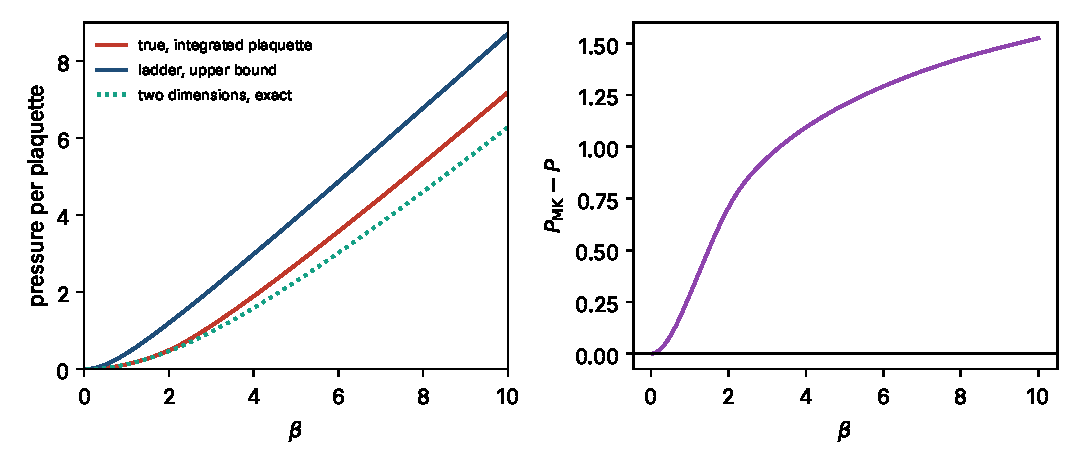
\includegraphics[width=\textwidth]{figures/kadanoff_bound.pdf}
\caption[Kadanoff's bound on the pressure]{Left: the pressure per plaquette of four dimensional SU(2), obtained by integrating the measured plaquette, the rigorous upper bound from the Migdal Kadanoff ladder, and the exact two dimensional pressure. Right: the gap between the ladder's bound and the truth.}
\label{fig:kadanoff}
\end{figure}

The bound holds, with a gap that grows slowly, from $0.3$ at $\beta=1$ to $1.5$ at $\beta=10$: at weak coupling both pressures grow like $\beta$ minus a multiple of $\log\beta$, with different multiples. The ladder's bound is a little better than the one obtained by integrating the heat bath bound $W_{11}\le u(2(d-1)\beta)$. The true pressure lies above the two dimensional one in every row (equal to three decimals at $\beta=1$), the integrated form of an inequality, $W_{11}^{(d)}\ge W_{11}^{(2)}$, that Ginibre's theorem gives for abelian groups and that is open for SU(2).

Kadanoff's bound is too weak to give a gap: a bound on a pressure does not bound a correlation length. But it fixes the direction of the ladder's error rigorously and at every scale. The moved system has more pressure than the true one; it is stiffer. Every numerical comparison in this chapter found the ladder on that side.

\subsection{What remains}

Three things. The bare inequality above, which would make the ladder's first step a rigorous upper caricature. The order between laws: the corollary and the theorem bound expectations, character by character on the independent side, and the likelihood ratio order supported by the data of the first half of this chapter asks for more. And iteration: a sandwich for expectations at one step does not control the next step unless it holds between laws in an order that the two operations of the ladder preserve, which is where Theorem~\ref{thm:tp2} and the bad cap enter.

\section*{Exercises}
\begin{enumerate}
\item Show that in two dimensions the measured and independent laws of the first section of this chapter coincide.
\item Show that in the Gaussian ledger a bond moving power $k$ followed by decimation with $b=2$ gives $\log W_{22}/\log W_{11}=4/k$.
\item Prove $W_{22}\ge W_{11}^4$ for $\Z_2$ gauge theory from Griffiths' second inequality (Section~\ref{ch:griffiths}).
\item Prove Griffiths' first inequality for the Ising model by expanding $e^{J\sigma_i\sigma_j}=\cosh J\,(1+\sigma_i\sigma_j\tanh J)$.
\item Verify the identity for $\cos a\pm\cos b$ and complete the proof of Theorem~\ref{thm:ginibre} for the plane rotator.
\item Show that in two dimensional SU(2) lattice gauge theory $W_{12}=W_{11}^2$, and identify the step of the proof of Theorem~\ref{thm:doubling} that is an equality there.
\item Use the proof of Theorem~\ref{thm:doubling}, with the Schwarz inequality for two different functions, and a plane that cuts a rectangular loop to prove $W_{R_1+R_2,T}^2\le W_{2R_1,T}\,W_{2R_2,T}$, the convexity of the static potential.
\item Extend Theorem~\ref{thm:heatbath} to SU(N), replacing $u$ by the mean of the fundamental character under the single link conditional (for SU(N) that conditional mean is not a scalar times a group element, so operator norms may be needed).
\item Compute $\log W_{12}/\log W_{11}$ in lowest order perturbation theory in four dimensions with the code of Appendix~\ref{ch:code}, extended from square to rectangular loops.
\end{enumerate}

\part{Neighbours}
\chapter{Neighbouring Problems}\label{ch:kacyang}\index{Kac, M.}\index{P\'olya, G.}\index{Yang, C. N.}\index{Lee Yang theorem}\index{Hilfssatz II}\index{Fisher zeros}

This chapter gathers problems next to the mass gap that share its mathematics. The first section takes from Kac and Yang a discrete system whose zeros can be located, and puts it in Thorin form (Chapter~\ref{ch:positivity}). The second reads stochastic quantisation and nonlinear filtering through the lattice Langevin equation and the Migdal Kadanoff ladder of Chapter~\ref{ch:strong}. The third reads our Hilbert sixth volume for what it says about the mass gap and what it supplies to the ladder. The last two take from our Riemann and Langlands volumes the tools, and the one negative result, that bear on this book.

\section{Kac, P\'olya and Yang: A Discrete System}

In the second volume of P\'olya's \emph{Collected Papers}, Mark Kac wrote a commentary~\cite{Ka74} on P\'olya's 1926 paper~\cite{Po26} on the integral representation of the Riemann $\xi$ function. It is three pages long. It records how a lemma from that paper, proved in pursuit of the Riemann Hypothesis, became an ingredient of the Lee and Yang circle theorem~\cite{LY52}, and it includes a recollection by C. N. Yang of the weeks in which the theorem was found. The Yang of that story is the Yang of Yang and Mills~\cite{YM54}, two years before their paper. This section tells the story, gives the mathematics, puts it in Thorin form following a 2026 note of the first author~\cite{Po26b}, and then does for Yang Mills what Kac did for the lattice gas: it looks at the smallest discrete system and asks where the zeros are.

\subsection{The commentary}

Kac begins by remarking that P\'olya's paper, though it comes very close to the Riemann Hypothesis, inspired little further work, and that it nevertheless played a small part in an important chapter of statistical mechanics. In late 1951 and early 1952 Lee and Yang were developing their theory of phase transitions and had been led, by examples, to a conjecture. For spins $\mu_k=\pm1$ and couplings $J_{kl}\ge0$, the function
\[
G_N(z)=\sum_{\mu}\exp\Big(\sum_{k,l=1}^NJ_{kl}\mu_k\mu_l\Big)\exp\Big(iz\sum_{k=1}^N\mu_k\Big)
\]
has only real zeros. When Kac heard of it he tried the simplest case, all couplings equal, and the second auxiliary theorem of P\'olya's paper, Hilfssatz II, came to his mind. He proved the conjecture in that case and showed the proof to Lee and Yang, who a couple of weeks later had the general theorem.

Yang's recollection, which Kac prints, fills in the rest. After about six weeks of failed attempts Kac showed them the equal coupling proof in early December, and around the twentieth Yang saw that by treating the fugacities of the sites as independent variables and following their motion relative to the unit circle, an induction of the same kind as Kac's would give everything. He calls the theorem ``a minor gem''~\cite[pp.~424 to 426]{Ka74}.

\subsection{Kac's proof}

Take $J_{kl}=\nu/2$ for all $k,l$, with $\nu>0$. Then the exponent depends on the spins only through $M=\sum\mu_k$, and adding one spin gives $\frac\nu2(M+\mu)^2+iz(M+\mu)=\frac\nu2M^2+(\nu\mu+iz)M+iz\mu+\frac\nu2$. Summing over the new spin,
\[
e^{-\nu/2}\,G_{N+1}(z)=e^{iz}\,G_N(z-i\nu)+e^{-iz}\,G_N(z+i\nu).
\]
The right side is P\'olya's operator. Hilfssatz II states that if $G$ is entire of genus at most one, real on the real axis, with only real zeros, then $e^{iz}G(z-i\nu)+e^{-iz}G(z+i\nu)$ has only real zeros. The proof, in Kac's form: at a zero $z=x+iy$ of the right side, $|e^{2iz}|^2=|G_N(z+i\nu)/G_N(z-i\nu)|^2$. If $G_N$ has real zeros $\alpha_n$, its Hadamard product gives
\[
e^{-4y}=\prod_n\frac{(\alpha_n-x)^2+(y+\nu)^2}{(\alpha_n-x)^2+(y-\nu)^2}.
\]
For $y>0$ every factor on the right exceeds one and the left side is below one; for $y<0$ the reverse. So $y=0$. The induction starts at $N=1$, where $G_1(z)=2e^{\nu/2}\cos z$.

We shall call this Kac's argument, and the displayed identity Kac's identity. It is an induction on the size of a discrete system, its engine is an operator that preserves a class of functions defined by where their zeros lie, and the reality of the zeros is proved by a comparison of signs that uses only the positivity of $\nu$, the ferromagnetic sign of the coupling.

\subsection{From one variable to many}

Kac's identity needs equal couplings, because only then does the new spin couple to the old ones through the single variable $M$. Yang's step was to give every site its own variable. With $z_k$ the fugacity of site $k$,
\[
\Phi_N(z_1,\dots,z_N)=\sum_{\mathcal I\subset\{1,\dots,N\}}W(\mathcal I)\prod_{k\in \mathcal I}z_k
\]
is a polynomial of degree one in each variable, and the claim becomes that $\Phi_N$ does not vanish when all $|z_k|<1$. Kac's function is the diagonal, $G_N(\zeta)=e^{iN\zeta}\Phi_N(w,\dots,w)$ with $w=e^{-2i\zeta}$, and real $\zeta$ is the unit circle. Adding a site gives $\Phi_{N+1}=P_0+z_{N+1}P_1$ with $P_0$ and $P_1$ of the same form, and the induction closes by a contraction lemma for polynomials of degree one in each of two variables, in the form later isolated by Asano~\cite{As70}: if $c_0+c_1z_1+c_2z_2+c_3z_1z_2$ has no zeros with both $|z_i|>1$, then $c_0+c_3z$ has none with $|z|>1$ (the form with $|z|<1$ follows by inversion). In this reading the circle theorem is Hilfssatz II carried from the line to the disc and applied one variable at a time.

\subsection{The Thorin form}

The bridge to this book is a rotation. If $G$ is even, of order one, with real zeros $\pm\alpha_n$, then $\tilde G(\sigma)=G(i\sigma)$ has $\tilde G(\sigma)/\tilde G(0)=\prod_n(1+\sigma^2/\alpha_n^2)$, and, factor by factor,
\[
\frac{G(0)}{G(i\sqrt s)}=\prod_n\Big(1+\frac{s}{\alpha_n^2}\Big)^{-1}=\E\,e^{-sH},\qquad H=\sum_n\frac{\mathcal E_n}{\alpha_n^2},
\]
with $\mathcal E_n$ independent standard exponentials. The reciprocal is the Laplace transform of a generalized gamma convolution~\cite{Th77,Bo92} whose Thorin measure is the counting measure $\sum_n\delta_{\alpha_n^2}$ on the squared zeros.

\begin{theorem}[Frullani bridge; Polson~\cite{Po26b}]\label{thm:frullani}
For $G$ even, entire of order one, real on the real axis, with $G(0)\ne0$, the following are equivalent: all zeros of $G$ are real; for every $\nu>0$ the zeros of $e^{iz}G(z-i\nu)+e^{-iz}G(z+i\nu)$ are real; and $G(0)/G(i\sqrt s)$ is the Laplace transform of a generalized gamma convolution, extending without zeros to the plane cut along the negative axis.
\end{theorem}

In this chapter only the implications from real zeros of $G$ to the other two conditions are used: the second is Hilfssatz II and the third is the displayed product. The converse implication is taken from~\cite{Po26b}; its proof, which needs the limit $\nu\to0$, is not reproduced here.

Kac's comparison of signs and Bondesson's theorem~\cite{Bo92} that the Laplace transform of a generalized gamma convolution has no zeros off the cut are two faces of one fact: the logarithm of $\tilde G$ is an integral of $1-e^{-\sigma^2s}$ against a positive measure. For a finite system the measure is atomic and the analytic continuation degenerates to a sign comparison. The Riemann Hypothesis, in the form of our Riemann volumes, is the same statement for a function whose Thorin measure is not known to be positive: the unbounded analogue of the circle theorem, with the inductive step missing.

Yang Mills sits on the other side of this bridge: in lattice gauge theory positivity of the spectral measure is free, by reflection positivity, and Section~\ref{ch:routeB} used the same Frullani identity, in the form of the $2\sin^2$ lemma, to transport it to a positive Thorin density. What is hard there is the support. The two problems that Yang's name is attached to are the two halves of one dictionary.

\subsection{Yang Mills as a discrete system: one plaquette}

Follow Kac and take the smallest system. For one plaquette of SU(2) lattice gauge theory the partition function in the weight $e^{\beta\cos\theta}$ is
\[
Z(\beta)=\int e^{\beta\cos\theta}\,\mathrm d\mathrm{Haar}=\frac{2I_1(\beta)}{\beta}.
\]
It is an even entire function of the coupling. Its zeros in the complex coupling, the Fisher zeros, are at $\beta=\pm i\,j_{1,n}$, with $j_{1,n}=3.832,\,7.016,\,10.173,\dots$ the positive zeros of the Bessel function $J_1$: all on the imaginary axis. So $Z$ is in exactly the rotated P\'olya class of the last subsection, and the bridge applies.

\begin{proposition}\label{prop:hitting}
For $\lambda>0$,
\[
\frac{1}{Z(\sqrt{2\lambda})}=\frac{\sqrt{2\lambda}}{2I_1(\sqrt{2\lambda})}=\prod_{n\ge1}\Big(1+\frac{2\lambda}{j_{1,n}^2}\Big)^{-1}=\E\,e^{-\lambda T},
\]
where $T$ is the first time that Brownian motion in $\R^4$, started at the origin, hits the unit sphere $S^3$, which is the group SU(2). The law of $T$ is a generalized gamma convolution with Thorin measure $\sum_n\delta_{j_{1,n}^2/2}$.
\end{proposition}

\begin{proof}
The radial part of Brownian motion in $\R^4$ is a Bessel process of index $a=1$, and the Laplace transform of its hitting time of one, started at zero, is $(\sqrt{2\lambda})^a/(2^a\Gamma(a+1)I_a(\sqrt{2\lambda}))$, by the classical results of Ciesielski and Taylor~\cite{CT62} and of Kent~\cite{Ke78}. The product is the Hadamard factorisation of $I_1(x)/x$.
\end{proof}

The proposition is the plaquette analogue of Kac's observation. The reciprocal of the Yang Mills partition function of one plaquette, as a function of the squared coupling, is the Laplace transform of a hitting time: the time for Brownian motion in the flat space in which the group sits as the unit sphere to reach the group. The same holds for U(1), the unit circle in the plane, with $I_0$ and $j_{0,n}$, and for any sphere. The Biane, Pitman and Yor variable~\cite{BPY} $S_{\mathrm{BPY}}$ of Section~\ref{ch:mk}, with transform $\sqrt{2\lambda}/\sinh\sqrt{2\lambda}$, is the member of the family with index $\frac12$, the hitting time of the two sphere. For a disc of $A$ plaquettes the partition function is $Z^A$ and its reciprocal is the transform of a sum of $A$ independent copies of $T$.

\subsection{A discrete system with complex zeros: the torus}

A disc of $A$ plaquettes in two dimensions has partition function $Z^A$, with the same zeros as one plaquette, and no dynamics; its plaquettes are independent. The smallest two dimensional system that is not a product is the torus, where the partition function is a sum over the characters of the group,
\[
Z_A(\beta)=\sum_{n\ge1}\Big(\frac{2I_n(\beta)}{\beta}\Big)^A ,
\]
with $A$ the number of plaquettes. We located its zeros numerically (Figure~\ref{fig:fisher}).

\begin{figure}[t]
\centering
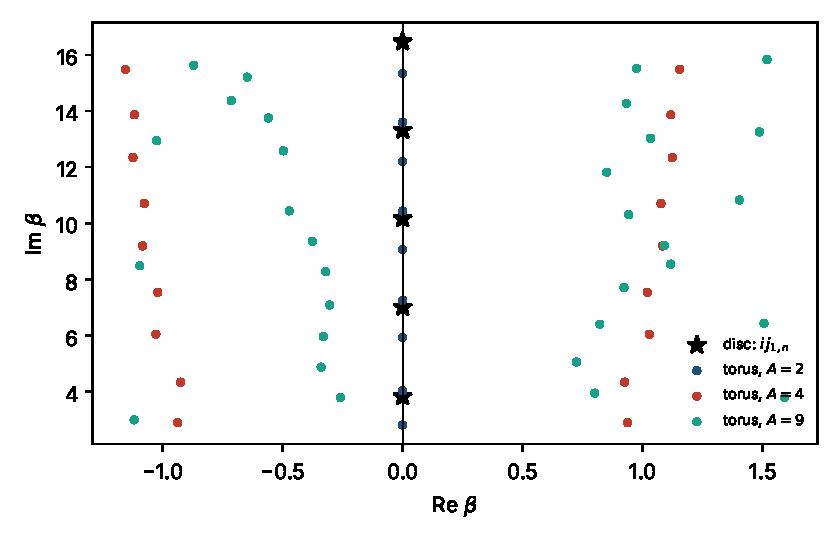
\includegraphics[width=0.55\textwidth]{figures/fisher_zeros.pdf}
\caption[Fisher zeros of two dimensional SU(2) lattice gauge theory]{Zeros in the upper half of the complex coupling plane of the partition function of two dimensional SU(2) lattice gauge theory: on a disc, where they lie on the imaginary axis at $i\,j_{1,n}$, and on tori of $2$, $4$ and $9$ plaquettes.}
\label{fig:fisher}
\end{figure}

For $A=2$ all zeros in the window $|\operatorname{Re}\beta|\le8$, $0<\operatorname{Im}\beta\le16$ lie on the imaginary axis. For $A=4$ and $A=9$ they do not: zeros appear with real parts up to $1.2$ and $1.6$. The closest to the real axis are at $-0.94+2.89i$ for $A=4$ and $-1.12+3.00i$ for $A=9$, against $3.83i$ for the disc. So the pure form of the property, all Fisher zeros imaginary, equivalently $Z(0)/Z(\sqrt s)$ the transform of a generalized gamma convolution, holds for the disc and, in the window searched, for the smallest torus, and fails for the larger tori computed. Nothing is wrong: in two dimensions the free energy per plaquette is $\log(2I_1(\beta)/\beta)$ in every infinite volume limit, analytic on the positive axis, and the zeros of the three tori we computed ($A=2$, $4$, $9$) stay a distance of about three from that axis. What the example shows is which form of the Lee and Yang property a gauge theory can be expected to have. It is not that the zeros lie on a line. It is that a neighbourhood of the positive real axis is free of zeros, uniformly in the volume.

In four dimensions that is the statement, assumed throughout this book, that there is no phase transition between strong and weak coupling; a Lee and Yang theorem for Yang Mills would be a proof that the Fisher zeros keep a fixed distance from the positive axis as the volume grows (Section~\ref{ch:missing}).

For the heat kernel action the question has an exact answer, and the reason is a scaling that Kac would have liked. On a torus of $A$ plaquettes with heat kernel weights $K_t$, the character coefficients are $e^{-(n^2-1)t/4}$, and
\[
Z_A(t)=\sum_{n\ge1}e^{-(n^2-1)At/4}=\mathcal G(q),\qquad q=e^{-At/4},
\]
where $\mathcal G(q)=1+q^3+q^8+q^{15}+\cdots=(\vartheta_3(q)-1)/(2q)$.
The partition function of every torus is one function of one variable.

\begin{theorem}[zeros on fixed rays]\label{thm:sector}
Let $q_1,q_2,\dots$ be the zeros of $\mathcal G$ in the unit disc and $s_j=-\log q_j$, with the principal logarithm. For two dimensional SU(2) lattice gauge theory with the heat kernel action on a torus of $A$ plaquettes, the zeros of the partition function in the complex time $t$, $\operatorname{Re}t>0$, are exactly $t=4(s_j+2\pi ik)/A$, $k\in\Z$. They lie on the same rays for every $A$, and $\mathcal G$ has no zeros in $|q|\le0.83$.
\end{theorem}

\begin{proof}
The identity for $Z_A$ is the definition, and $q=e^{-At/4}$ is a zero of $\mathcal G$ exactly when $At/4=s_j+2\pi ik$. For $|q|\le0.83$, $|\mathcal G(q)-1|\le|q|^3/(1-|q|^5)<1$.
\end{proof}

\paragraph{\normalfont\scshape A numerical result.} The sector $|\arg t|<\phi_*$, equivalently $|\arg\beta|<\phi_*$ for $\beta=2/t$, with $\phi_*=\inf_j|\arg s_j|$, contains no zero for any $A$. Numerically the zeros of $\mathcal G$ of smallest modulus are
\[
q_1=0.3888+0.7793\,i,\qquad q_2=-0.8669+0.2999\,i,
\]
with $|\arg s_1|=82.9^\circ$ and $|\arg s_2|=88.2^\circ$, so that $\phi_*=82.9^\circ$. The script \texttt{code/torus\_sector.py} counts the zeros of $\mathcal G$ by the argument principle on circles, finding $2$, $4$ and $82$ zeros in $|q|<0.9$, $0.95$ and $0.997$, and finds the same $41$ zeros in the upper half plane by Newton's method. In the closed sector the modular identity $\vartheta_3(e^{-s})=\sqrt{\pi/s}\,\vartheta_3(e^{-\pi^2/s})$ gives $|\vartheta_3(e^{-s})|\ge1.11$ for $|s|\le0.8$, and for $|s|\ge0.8$ the sector lies in $|q|\le0.906$, where $q_1$ and its conjugate are the only zeros. This is a floating point computation, not a certified one, and we do not call it a proof.

\begin{figure}[t]
\centering
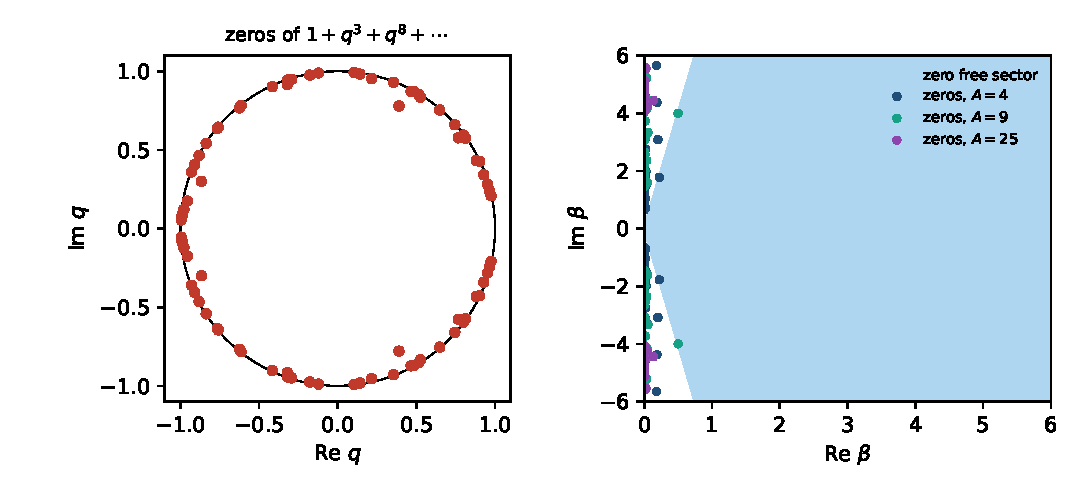
\includegraphics[width=0.75\textwidth]{figures/torus_sector.pdf}
\caption[A numerical zero free sector for the heat kernel torus]{Left: the zeros of $\mathcal G(q)=1+q^3+q^8+\cdots$ in the unit disc with $|q|\le0.997$. Right: the corresponding Fisher zeros in the coupling $\beta=2/t$ for tori of $4$, $9$ and $25$ plaquettes, all outside the sector of half angle $82.9^\circ$ around the positive axis.}
\label{fig:torussector}
\end{figure}

So for the heat kernel action in two dimensions the computation shows the Lee and Yang property in the form that matters: the zeros are confined, for every volume at once, to within about seven degrees of the imaginary axis (Figure~\ref{fig:torussector}), by a numerical value of the angle and not by a proof. The Wilson action lacks the scaling, and its zeros, shown in Figure~\ref{fig:fisher}, wander further.

\begin{problem}\label{op:neigh1}
Prove a zero free sector around the positive axis, uniform in the volume, for the Wilson action on two dimensional tori, and for the partition function on hierarchical lattices, where the Migdal Kadanoff recursion acts on the zeros as P\'olya's operator acts in Kac's proof.
\end{problem}

\subsection{What is due to Kac}

The observation that P\'olya's Hilfssatz II, a lemma about the Riemann $\xi$ function, proves a theorem of statistical mechanics is Kac's, and so is the proof of the circle theorem for equal couplings, the first proof of any case of it. The identity that compares $e^{-4y}$ with a product over the zeros, which the Frullani bridge identifies with the positivity of a Thorin measure, is his. And the method is his: when faced with a hard conjecture about a large system, take the smallest case, the most symmetric coupling, and a single variable, and find the mechanism there. Proposition~\ref{prop:hitting} and Theorem~\ref{thm:sector} are that method applied to one plaquette and to a torus.

The idea that organises our whole approach to four dimensions, that an exactly solvable caricature can carry the truth of a hard problem, is the thesis of his essay on models~\cite{Ka69}. This book treats the Migdal Kadanoff ladder as a caricature in exactly his sense.

Kac wrote his commentary to give credit to P\'olya for a paper that had been little noticed, and took care to print Yang's own account beside his. We have tried to follow that example.

\section{Stochastic Quantisation, Filtering and the Ladder}\label{ch:spde}\index{stochastic quantisation}\index{stochastic partial differential equation}\index{Hairer, M.}\index{regularity structures}\index{Zakai equation}\index{Kushner Stratonovich equation}\index{Kurtz, T. G.}\index{Xiong, J.}\index{particle filter}

Section~\ref{ch:probabilists} named the probabilists who work on gauge fields. We return to them with the rest of the book in hand, and ask of each line of work the question we have asked of everything else: what does it say about the gap? We have read the abstracts, introductions and statements of main results of the papers cited, not their proofs, and we report them at that level.

\subsection{The Langevin equation of a gauge field}\index{Parisi, G.}\index{Langevin dynamics}

Parisi and Wu~\cite{PW81} proposed in 1981 to construct a Euclidean field theory as the invariant law of a diffusion: the gradient flow of the action, driven by white noise in space and a fictitious time. For a gauge field $A$ with curvature $F_A$ the equation is
\[
\partial_\tau A=-D_A^*F_A+\xi ,
\]
with $\xi$ a space time white noise with values in the Lie algebra. Two things make it hard. The noise is rough, so that $A$ is a distribution and the quadratic and cubic terms of $D_A^*F_A$ are products of distributions; and the equation is covariant under gauge transformations, so that it is parabolic only after a gauge is fixed, by the device of DeTurck~\cite{DT83}.

On a lattice none of this is singular, and the equation is a system of interacting diffusions, one for each link:
\[
dU_\ell=-\tfrac\beta2\nabla_\ell S(U)\,d\tau+dB_\ell ,
\]
where $B_\ell$ are independent Brownian motions on the group and $\nabla_\ell S$ is the gradient of the Wilson action with respect to the link, a function of its staples. Its invariant law is the Wilson measure. It is a continuous time relative of the heat bath algorithm of Section~\ref{ch:latticemc}, with the same invariant law, and its spectral gap is the dynamic gap of Section~\ref{ch:dynamic}.

\subsection{What has been constructed}

\paragraph{\normalfont\scshape Two dimensions.} Chandra, Chevyrev, Hairer and Shen~\cite{CCHS} constructed the Langevin dynamic of the two dimensional Yang Mills measure on the torus with Hairer's regularity structures~\cite{Ha14}: a state space of distributional connections on which holonomies along smooth curves make sense, local solutions, and gauge covariance in law after renormalisation. Chevyrev and Shen~\cite{ChSh23} then proved that the two dimensional Yang Mills measure is invariant for the renormalised dynamic, for any connected compact structure group, by passing through the lattice and Bourgain's method~\cite{Bo96} for invariant measures, and derived a universality statement for lattice actions.

\paragraph{\normalfont\scshape Two dimensions with matter.} Bringmann, Cao, Hairer and Zhao~\cite{BCHZ} constructed the nonabelian Yang Mills Higgs measure on the two dimensional torus by stochastic quantisation alone. It holds for any fixed couplings. No rate of convergence and no mass gap is claimed.

\paragraph{\normalfont\scshape Three dimensions.} Chandra, Chevyrev, Hairer and Shen~\cite{CCHS3} defined a state space and a Markov process on gauge orbits for the stochastic quantisation of Yang Mills Higgs in three dimensions, up to a possible blow up in finite time, with a unique choice of counterterms that makes the solution gauge covariant in law. The measure in three dimensions has not been constructed this way.

\paragraph{\normalfont\scshape Four dimensions.} The equation is critical in four dimensions, in the sense of regularity structures, and no local theory exists. This is the stochastic face of asymptotic freedom: the nonlinearity is not small at small scales by power counting, only by a logarithm.

\subsection{One plaquette, exactly}\index{Bakry \'Emery criterion}

The dynamic route can be seen in full on the smallest example. Take one plaquette, that is one group element $U$ with law proportional to $e^{\beta\cos\theta}$ times Haar measure, and its Langevin equation with generator $L=\frac12\Delta+\frac\beta2\nabla\cos\theta\cdot\nabla$. On the unit sphere $S^3$ the Ricci curvature is $2$ and the Hessian of $a_0=\cos\theta$ is $-a_0$ times the metric, so the Bakry \'Emery~\cite{BE} curvature is
\[
\tfrac12\big(2+\beta\cos\theta\big)\ \ge\ 1-\frac\beta2 ,
\]
and the criterion gives a gap of at least $1-\beta/2$ for $\beta<2$ and nothing beyond. The true spectrum is easy to compute. The generator commutes with rotations about the identity, its eigenfunctions split by angular momentum $l$, and each sector is a Sturm Liouville problem in $\theta$.

\begin{center}
\small
\begin{tabular}{cccccccc}
\toprule
$\beta$ & 0 & 1 & 2 & 4 & 6 & 8 & 12 \\ \midrule
$l=0$ & 1.500 & 1.600 & 1.897 & 3.051 & 4.809 & 6.848 & 10.93 \\
$l=1$ & 1.500 & 1.566 & 1.758 & 2.439 & 3.337 & 4.304 & 6.282 \\
bound & 1.00 & 0.50 & 0.00 & $-1.00$ & $-2.00$ & $-3.00$ & $-5.00$ \\
\bottomrule
\end{tabular}
\end{center}
The rows are the lowest nonzero rate among class functions, the lowest rate in the sector $l=1$, which is the gap among the sectors computed (the sectors $l\ge2$ were not), and the Bakry \'Emery bound.

\begin{figure}[t]
\centering
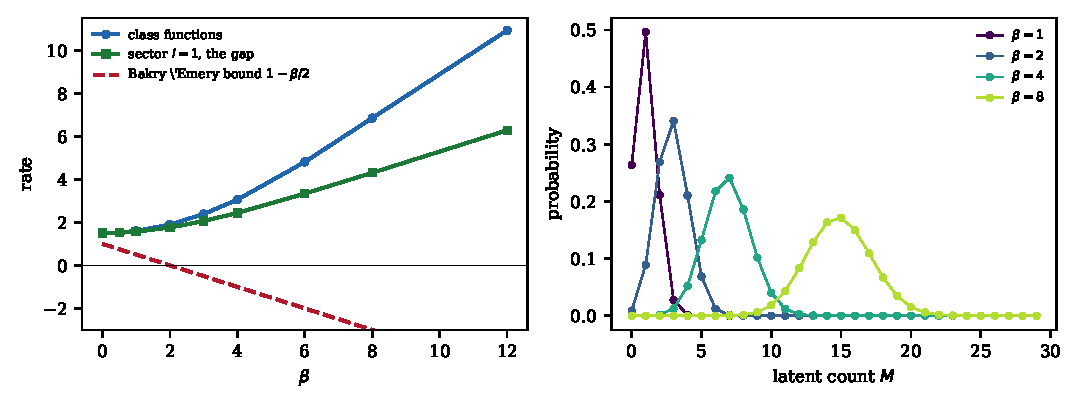
\includegraphics[width=0.75\textwidth]{figures/langevin_latent.pdf}
\caption[One plaquette Langevin gaps and the latent count]{Left: the spectral gap of the Langevin dynamic of one SU(2) plaquette in the sectors $l=0$ and $l=1$, and the Bakry \'Emery lower bound, which becomes void at $\beta=2$ while the gap grows. Right: the law of the latent count $M$ of Section~\ref{ch:langlands} for the heat kernel at four couplings.}
\label{fig:langevinlatent}
\end{figure}

The gap grows with $\beta$, like $\beta/2$, because near the identity the dynamic is an Ornstein Uhlenbeck process with that rate. The bound falls with $\beta$ and is void from $\beta=2$ on (Figure~\ref{fig:langevinlatent}). The reason is instructive. The bound is a minimum over the group, attained at the antipode, where the potential is concave. The measure gives the antipode weight of order $e^{-2\beta}$. So the criterion fails because of a region that the measure does not see.

This is the bad cap of Chapter~\ref{ch:progress} in another guise. There, total positivity of the convolution kernel failed in a cap at the antipode of small mass; here, uniform convexity fails in a cap at the same antipode. In both, a pointwise criterion is defeated by a set of negligible measure, and the remedy must be a criterion that averages, a Poincar\'e inequality proved by a Lyapunov function and a local inequality in the manner of Bakry, Cattiaux and Guillin~\cite{BCG08}. The single plaquette shows that the failure of the criterion is not evidence against a gap.

\subsection{What this says about the gap}

Two readings, in increasing order of relevance to this book.

First, the existence results are about the ultraviolet. They are the dynamic counterpart of Ba\l aban's stability bounds: control uniform in the cutoff at a fixed physical scale. The gap is an infrared statement. In our language, the stochastic quantisation programme constructs the measure and is silent, so far, on its support.

Second, where the dynamics has a gap, the measure has one. Shen, Zhu and Zhu~\cite{SZZ} proved on the lattice at strong coupling that the Langevin dynamic satisfies the Bakry \'Emery condition, hence a log Sobolev inequality uniform in the volume, hence exponential decay of correlations and a mass gap, with large $N$ consequences. This is the dynamic route of Section~\ref{ch:dynamic} carried out where curvature of the group beats the Hessian of the action. Cao, Nissim and Sheffield~\cite{CNS25} extended the regime in which the area law is proved for $U(N)$ lattice theories, in particular at large $N$, improving on Osterwalder and Seiler~\cite{OSe}, and gave a sufficient condition for the area law in terms of a strong enough mass gap; a companion paper takes a dynamical approach. The direction of that implication, from a gap to an area law, is the one this book has not used and should: our ladder gives the string tension first and the gap second.

Other work on the list of Section~\ref{ch:probabilists}: two dimensional Yang Mills as Brownian motion on the group indexed by area (Gross, King and Sengupta~\cite{GKS89}, Sengupta~\cite{Se97}, L\'evy~\cite{Le03}), on which everything exact in this book rests; Chatterjee's survey~\cite{Ch19}; and the surface expansions of Wilson loops of Cao, Park and Sheffield~\cite{CPS25}, whose signs are the obstruction to a probabilistic reading. The ground state representation of Proposition~\ref{prop:groundstate} is the picture of Nelson~\cite{Ne73} and Gross~\cite{Gro75} applied to a gauge field.

The stochastic quantisation programme and this book meet at one object, the lattice Langevin equation, and look at it from opposite ends. They take the lattice spacing to zero at fixed size and ask whether the dynamics survives. We fix the lattice, block it, and ask where the coupling goes. A proof of the gap would need both: their uniformity in the cutoff, and a statement like ours, on the real lattice, that blocking moves the effective law toward the region where the dynamics is known to contract.

\subsection{Filtering and the ladder in continuous scale}\label{ch:spdefilter}

There is a second family of stochastic equations, older in statistics, in which the unknown is a probability law: the equations of nonlinear filtering. The link is the interacting particle system, which is a numerical method for a filtering equation, by Kurtz and Xiong a representation of its solution, and, for a lattice gauge field, the Langevin equation itself. Chapter 20 of our Hilbert sixth book~\cite{PS26h} treats the filtering side; here we add what the gauge theory needs, and one formula, the ladder in continuous scale.

A signal $X_s$ diffuses with generator $L$ and is observed through $dY_s=h(X_s)\,ds+dV_s$. The unnormalised conditional density $\varrho_s$ of the signal given the observations solves Zakai's linear equation~\cite{Za69}, and the normalised law $\pi_s$ solves the nonlinear equation of Kushner and Stratonovich~\cite{Ku64,St60}:
\begin{align*}
d\varrho_s&=L^*\varrho_s\,ds+\varrho_s\,h\,dY_s,\\
d\pi_s(f)&=\pi_s(Lf)\,ds+\big(\pi_s(h f)-\pi_s(h)\pi_s(f)\big)\big(dY_s-\pi_s(h)\,ds\big).
\end{align*}
Two operations alternate, in continuous time: prediction by the Fokker Planck flow, and correction by a likelihood. The correction term is a covariance: the law moves in the direction in which $f$ is correlated with the log likelihood. A particle filter is the Monte Carlo form: move the particles by the signal dynamics, weight them by the likelihood, resample.

Kurtz and Xiong~\cite{KX99} turned the algorithm into a theorem: for an infinite exchangeable system of weighted particles sharing a common noise, the weighted empirical measure is the unique solution of a nonlinear stochastic partial differential equation in a class that contains the Zakai and Kushner Stratonovich equations, with the observation as common noise, and the McKean Vlasov equation, with no common noise. Later work gives error bounds~\cite{KX01}, Gaussian fluctuations~\cite{KX04} and boundary conditions~\cite{CJK18}.

The lattice Langevin equation is a system of interacting diffusions on the group with independent noises, no common noise and no exchangeability, only translation invariance, so the Kurtz Xiong theorem does not apply to it as it stands. We use the filtering equations as an analogy for the Migdal Kadanoff ladder, which is a filter in scale: Section~\ref{ch:plgbc} called bond moving the update and decimation the prediction. The next formula makes the scale continuous and finds the Kushner Stratonovich form exactly, without noise.

\index{beta function}
Let the scale factor be $b=1+d\varsigma$. Bond moving raises the density to the power $b^{d-2}=1+(d-2)\,d\varsigma$, and decimation takes the convolution power $b^2=1+2\,d\varsigma$. To first order in $d\varsigma$ the law $\rho_\varsigma$ of a link therefore satisfies
\[
\partial_\varsigma\rho=(d-2)\,\rho\,\big(\log\rho-\langle\log\rho\rangle_\rho\big)+2\,\mathcal C\rho ,
\]
where $\mathcal C\rho$ is the generator of convolution powers, which multiplies the character coefficient $u_n$ by $\log u_n$; on the heat kernel family $\mathcal C K_t=t\,\partial_tK_t$. This has the form of the Kushner Stratonovich equation with the noise removed, the innovation $dY_s-\pi_s(h)\,ds$ being replaced by $(d-2)\,d\varsigma$: the first term is a Bayes correction in which the law is its own likelihood, with rate $d-2$, and the second is a prediction. The correction term changes the mean of any $f$ at the rate $(d-2)\operatorname{Cov}_\rho(f,\log\rho)$.

\begin{proposition}[the projected ladder in continuous scale]\label{prop:contladder}
For SU(2), project onto the heat kernel family by the fundamental coefficient $u_2=e^{-3t/4}$ after each infinitesimal step. Then
\[
\frac{dt}{d\varsigma}=(4-d)\,t+(d-2)\,\mathcal B(t),\qquad\mathcal B(t)=t-\tfrac43e^{3t/4}\operatorname{Cov}_{K_t}\!\big(\cos\theta,\log K_t\big).
\]
\begin{enumerate}
\item[(i)] $\mathcal B(t)>0$ for every $t>0$.
\end{enumerate}
If the remainder in Theorem~\ref{thm:expansion} is $O((k-1)t^4)$, then
\begin{enumerate}
\item[(ii)] $\mathcal B(t)=\frac{t^2}6+\frac{t^3}{36}+\frac{t^4}{432}+O(t^5)$.
\item[(iii)] In four dimensions, with $\beta=2/t$, $\ \dfrac{d\beta}{d\varsigma}=-\dfrac23\Big(1+\dfrac1{3\beta}+\dfrac1{18\beta^2}+\cdots\Big)$.
\end{enumerate}
\end{proposition}

\begin{proof}
With $s(k)$ defined by $e^{-3s/4}=\int\cos\theta\,K_t^k/\int K_t^k$, differentiation at $k=1$ gives $s'(1)=-\frac43e^{3t/4}\operatorname{Cov}_{K_t}(\cos\theta,\log K_t)$. One step is $t\mapsto b^2s(b^{d-2})$, and expanding in $d\varsigma$ gives the formula. (i) Differentiating $e^{-3t/4}=\langle\cos\theta\rangle_{K_t}$ in $t$ gives $\frac34te^{-3t/4}=-\operatorname{Cov}_{K_t}(\cos\theta,t\,\partial_t\log K_t)$, so $\mathcal B(t)=-\frac43e^{3t/4}\operatorname{Cov}_{K_t}\big(\cos\theta,\partial_t(t\log K_t)\big)$. By Theorem~\ref{thm:scaledmlr} and Proposition~\ref{prop:initial}, $\partial_t(t\log K_t)$ is strictly decreasing in $\cos\theta$, and the covariance of an increasing and a strictly decreasing function of the same variable is negative. (ii) and (iii) are Theorem~\ref{thm:expansion} with $1-1/k=(d-2)\,d\varsigma$ and $k\to1$, which needs the $O(t^4)$ remainder there to be $O((k-1)t^4)$; the theorem does not state this, so (ii) and (iii) are conditional on it.
\end{proof}

On the real lattice the effective law of a block link depends on the neighbouring blocks, which is a common noise in the sense of Kurtz and Xiong; a stochastic ladder with such a noise is the natural extension, and we have not pursued it. The filtering form gives the ladder's beta function as a covariance, with the sign from Theorem~\ref{thm:scaledmlr}. None of it is a proof of the gap.

\section{Quantum Yang Mills and Hilbert's Sixth Problem}\label{ch:h6ym}\index{Hilbert's sixth problem}\index{Nelson, E.}\index{Feynman Kac formula}\index{ground state measure}\index{L\'evy area}\index{particle filter}\index{random walk on a group}

Our book \emph{On Hilbert's 6th Problem: Probability, Mechanics and Bayesian Computation}~\cite{PS26h} follows Hilbert's programme from Kolmogorov's axioms to the Navier Stokes equations and back, reading the inverse passage as Bayesian computation. Its last chapter contains a section on Yang Mills, written when the existence proof was announced, and several of its theorems are tools this book uses. Section and theorem numbers below refer to its version 1.1.0.

\subsection{Quantum field theory as a form of the sixth problem}

Hilbert asked in 1900 for a mathematical treatment of the axioms of physics, beginning with probability and mechanics. Its Section 9.6 places quantum field theory in the same frame: Wick rotation turns the Schr\"odinger group into the heat semigroup; Osterwalder and Schrader~\cite{OS} gave axioms for Euclidean Green functions in 1973, corrected in 1975 by a linear growth condition, under which the Euclidean theory continues to a relativistic one satisfying Wightman's axioms~\cite{SW64}; Nelson~\cite{Ne73} showed that Euclidean free fields are Markov fields; and Glimm and Jaffe~\cite{GJ} built interacting theories in two and three dimensions that way.

Quantum Yang Mills is that programme in its hardest case: existence was announced in 2026 and endorsed by a review group~\cite{OAI}, with ultraviolet stability by Ba\l aban~\cite{Ba87}, and the mass gap is the open statement about the long range behaviour of a measure whose short range behaviour is under control.

\subsection{Feynman Kac: the gap is a decay rate}

Theorem 9.4 of the Hilbert sixth book is the Feynman Kac formula: for $H=-\frac12\Delta+V$, the solution of the imaginary time equation is $\E_x\big[f(B_\tau)\exp(-\int_0^\tau V(B_s)\,\mathrm ds)\big]$. The ground state energy is the exponential decay rate of that expectation, and by the Donsker and Varadhan theory~\cite{DV75} a large deviation rate.

For Yang Mills in the Hamiltonian formulation of Kogut and Susskind~\cite{KS75}, the configuration space is a product of copies of SU(2), one for each spatial link, restricted to gauge invariant functions; the kinetic term is $g^2/(2a)$ times the sum of the quadratic Casimir operators of the group factors, each a Laplacian normalised to have eigenvalue $\frac34$ on the fundamental character; and the potential is a sum of spatial plaquette terms with a coefficient proportional to $1/(g^2a)$. In two spacetime dimensions there are no spatial plaquettes, the potential vanishes, the path measure is Brownian motion on the group, and the gap is the first eigenvalue of the Laplacian: the solution of Chapter~\ref{ch:twod}, read as the simplest case of Theorem 9.4.

The mass gap is the difference of two decay rates, $E_1-E_0$. Route B of this book is the statement that after the $2\sin^2$ transport that difference is itself a decay rate, of a positive Thorin density.

\subsection{Nelson: the gap is a Poincar\'e constant}

Section 9.5 of the Hilbert sixth book presents Nelson's stochastic mechanics~\cite{Ne66}: to a state $\psi$ corresponds a diffusion with drift $\nabla\log|\psi|$ and stationary law $|\psi|^2$, and its worked example, the harmonic oscillator, has the Ornstein Uhlenbeck process as the ground state diffusion. That picture gives a clean form of the mass gap.

\begin{proposition}[ground state representation]\label{prop:groundstate}
Let $H=-\frac{\kappa}{2}\Delta+V$ on a compact Riemannian manifold have a positive ground state $\Omega$ with energy $E_0$. The map $f\mapsto f\Omega$ carries $H-E_0$ on $L^2(\mathrm dx)$ to the operator
\[
L=-\frac\kappa2\Delta-\kappa\,\nabla\log\Omega\cdot\nabla\qquad\text{on }L^2(\Omega^2\mathrm dx),
\]
the generator of a reversible diffusion with invariant law $\mu=\Omega^2\mathrm dx$. Consequently
\[
E_1-E_0=\frac\kappa2\,\inf_f\frac{\int|\nabla f|^2\,\mathrm d\mu}{\operatorname{Var}_\mu(f)} :
\]
the gap is $\kappa/2$ times the reciprocal of the Poincar\'e constant of the ground state measure.
\end{proposition}

\begin{proof}
For smooth $f$, $H(f\Omega)=f\,H\Omega-\frac\kappa2\big(\Omega\Delta f+2\nabla f\cdot\nabla\Omega\big)=E_0f\Omega+\Omega\,Lf$. Integration by parts gives $\int f\,Lf\,\mathrm d\mu=\frac\kappa2\int|\nabla f|^2\mathrm d\mu$. The map is unitary from $L^2(\mu)$ to $L^2(\mathrm dx)$ and sends constants to the ground state, so the gap of $H$ is the smallest nonzero eigenvalue of $L$, which is the stated variational quotient.
\end{proof}

For lattice Yang Mills the manifold is the product of the groups on the spatial links, $\kappa=g^2/a$, and the mass gap is the rate at which Nelson's ground state diffusion on the space of spatial gauge fields forgets its initial condition. One remark connects this to the rest of the book.

At weak coupling the long wavelength form of $\Omega$ is the subject of an old conjecture of Greensite~\cite{Gr79}: for slowly varying fields, $\Omega^2$ is approximately $\exp(-\mathrm{const}\int\operatorname{tr}\mathbf b^2)$, the Yang Mills measure in one dimension less. If so, the Poincar\'e inequality for the ground state of the four dimensional theory is, at long distances, a mixing statement for the three dimensional Euclidean theory, and that of the three dimensional theory one for the two dimensional theory, which is solved. Karabali, Kim and Nair~\cite{KKN} computed an approximate form of it in three dimensions with an explicit kernel (Section~\ref{ch:threed}). The ladder of dimensions is a second ladder, across the one in scale, and it is another reason to do three dimensions first.

Diffusion Monte Carlo (Section 9.11), in which Brownian walkers are killed or duplicated at a rate set by the potential, is a particle filter in imaginary time with the potential as likelihood, the Hamiltonian counterpart of the particle ladder below, a filter in scale. Section 22.8 states the shape of the existence problem in the language of this book: a Gibbs measure on link variables with Haar reference measure, weak convergence of the laws of Wilson loops, a renormalization step as a marginal with the fine field integrated out as a latent variable, and, in the sentence that could stand as the epigraph of this book, ``positivity is free and the support is hard.''  Reading it for Yang Mills gives the mass gap three equivalent forms, each attached to a theorem of that book: a decay rate, by Feynman Kac; a Poincar\'e constant of the ground state measure, by Nelson's stochastic mechanics; and a support statement for a positive measure, by reflection positivity. This book adds a fourth, the decay rate of a Thorin density.

\subsection{What the Hilbert sixth book contributes to the ladder}\label{ch:h6}

Three of its results enter the ladder with no further work.

\paragraph{\normalfont\scshape The Brownian reading of $11/3$.}
Section 22.8 also gives a Brownian derivation of the one loop coefficient. In a constant background field $F$ the diagonal of the covariant heat kernel is the free one times $Fs/\sinh(Fs)=1-(Fs)^2/6+\cdots$, which is the characteristic function of L\'evy's stochastic area of a Brownian loop, while the spin of the gluon contributes $2\cosh(2Fs)=2+4(Fs)^2+\cdots$. The product is $2+\frac{11}{3}(Fs)^2$, so the one loop coefficient is

\[
N\Big(4-\frac13\Big):
\]
the magnetic moment of a spin one loop outweighs the area it encloses.

Compare Remarks~\ref{prop:decrementB} and~\ref{prop:sunB}. The ladder's decrement is $(1-b^{-2})N^2\E S_{\mathrm{BPY}}/4$, where $S_{\mathrm{BPY}}$ has Laplace transform $\sqrt{2\lambda}/\sinh\sqrt{2\lambda}$ and $\E S_{\mathrm{BPY}}=1/3$. With $x=\sqrt{2\lambda}$ this is the same function, $x/\sinh x=1-x^2/6+\cdots$. The number $1/3$ in the background field computation and the number $\E S_{\mathrm{BPY}}=1/3$ in the ladder are the mean of one law, read once as L\'evy's area and once as the curvature correction of the heat kernel on the group.

\begin{problem}\label{op:neigh2}
Explain why the Migdal Kadanoff decrement, built from $\E S_{\mathrm{BPY}}=1/3$ alone, reproduces at $b=2$, to three percent, a coefficient that the background field computation writes as $4-\frac13$. Is there a version of the ladder in which the terms $4$ and $-\frac13$ appear separately, and does it have the correct two loop coefficient?
\end{problem}

\paragraph{\normalfont\scshape Random walks on groups.}
Its Theorem 2.6 is the convergence theorem for random walks on finite groups, with the Fourier bound of Diaconis and Shahshahani~\cite{DS81}
\[
\|Q^{*n}-U\|_{\mathrm{TV}}^2\le\frac14\sum_{\rho\ne1}d_\rho\operatorname{tr}\big(\hat Q(\rho)^n(\hat Q(\rho)^n)^*\big)
\]
over nontrivial irreducible representations. On a compact group the same bound holds for laws with square integrable densities, and for a class function law on SU(2) with character coefficients $u_n$ it reads
\[
\|Q^{*m}-\mathrm{Haar}\|_{\mathrm{TV}}^2\le\frac14\sum_{n\ge2}n^2u_n^{2m} .
\]
Decimation in the ladder is exactly such a convolution power, with $m=b^2$. So the theorem measures, at each rung, how far the plaquette law is from Haar measure, that is, how far the rung is from the strong coupling fixed point. For the heat kernel law, $u_n=e^{-(n^2-1)/(2\beta)}$, and with $m=4$ the bound on the squared distance is below $10^{-2}$ once $\beta<2.6$. Poincar\'e's card shuffling and the decimation half of the ladder's approach to confinement are one theorem.

\paragraph{\normalfont\scshape The ladder is a filter.} 
The filtering chapter treats the particle filter as an interacting particle system. For a sequence of Bayes updates $\Psi_n$ and a Markov move $M$, it defines the McKean kernel $K_{n,\eta}=\Psi_n(\eta)M$, and its Proposition 20.4 shows that the time marginals of the resulting nonlinear Markov chain are the predictive laws; the bootstrap filter is its mean field particle approximation and propagates chaos.

The Migdal Kadanoff step has exactly this form. Let $\eta$ be the current plaquette law with density $f$ with respect to Haar measure.
\begin{itemize}
\item Update. Bond moving replaces $f$ by $f^k/\int f^k$. This is a Bayes update of the prior $\eta$ by the likelihood $f^{k-1}$, the law's own density.
\item Predict. Decimation replaces the law by its $b^2$ fold convolution, a Markov move on the group.
\end{itemize}
So the ladder is a nonlinear Markov chain of McKean type on SU(2), in which the likelihood at each step is a power of the current law. Proposition 20.4 says its time marginals are the plaquette laws of the ladder, and the particle filter is a simulation method for it: carry a cloud of group elements, estimate the density from the cloud, reweight and resample, then multiply independent draws.

\begin{figure}[t]
\centering
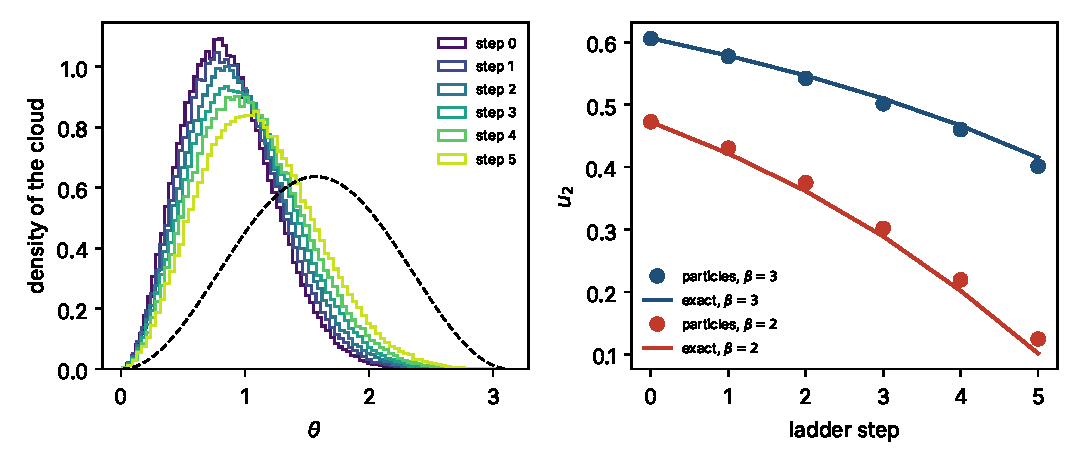
\includegraphics[width=0.75\textwidth]{figures/particle_mk.pdf}
\caption[The particle Migdal Kadanoff ladder]{The ladder run as a particle filter with $2\times10^5$ elements of SU(2), started from the heat kernel law. Left: the law of the rotation angle of the cloud over five steps from $\beta=3$, spreading toward the Haar density (dashed). Right: the second character coefficient of the cloud, points, against the exact flow, lines, from $\beta=3$ and $\beta=2$.}
\label{fig:particlemk}
\end{figure}

We implemented it (Figure~\ref{fig:particlemk}). With $2\times10^5$ particles, the density estimated from the first fourteen characters of the cloud, and $b=2$, the second character coefficient follows the exact flow to within $0.014$ over five steps from $\beta=3$ and to within $0.023$ from $\beta=2$. The errors grow along the ladder, as the error analysis of Section 20.4 of the Hilbert sixth book predicts for particle filters, because each update compounds the Monte Carlo error of the last.

The particle form needs no character expansion of the map, only samples and a density estimate, so it would apply to SU(3) and to block spin maps for which no closed recursion exists, subject to the accuracy of the density estimate at weak coupling and to degeneracy of the weights.

\section{What the Riemann Volumes Contribute}\label{ch:rhbooks}\index{Riemann Hypothesis}\index{de Bruijn Newman flow}\index{certified computation}\index{generalized gamma convolution}\index{Thorin measure}

This book is a sibling of our volumes \emph{Computing the Riemann Hypothesis}~\cite{PS26a,PS26b,PS26c}: Volume I, \emph{Representations of Xi, Thorin Measures and the Reciprocal Xi Function}; Volume II, \emph{Cauchy Deconvolution and Certified Computation}; and Volume III, \emph{Is There a Path?} Those volumes restate the Riemann Hypothesis as the positivity of a measure, the Thorin measure of a ratio of values of Riemann's $\Xi$ function, and they claim no proof. On 20 November 2026 L. Alp\"oge announced, with Lean code, a proof of the Riemann hypothesis and of the generalized Riemann hypothesis for Dirichlet $L$ functions~\cite{Alp26}. We have not examined it, and nothing in this book depends on it.

The programme starts from the reciprocal of Riemann's function $\xi(s)=\frac12s(s-1)\pi^{-s/2}\Gamma(s/2)\zeta(s)$, which is entire, satisfies $\xi(s)=\xi(1-s)$ and has Hadamard product $\xi(s)=\xi(0)\prod_\rho(1-s/\rho)$ over the zeros $\rho=\frac12+i\gamma$; the Riemann Hypothesis is the statement that every $\gamma$ is real. To the right of the zeros $1/\xi$ behaves like a Laplace transform, and one asks whether it is the Laplace transform of a generalized gamma convolution. The Euler product gives a L\'evy measure with atoms at $k\log p$ and the gamma factor a smooth part, so the question is the sign of a transported Thorin measure. Far to the right the Euler product converges absolutely and the Thorin structure is unconditional. At the centre of the strip the formal Thorin measure of the reciprocal is the sum of point masses at $\gamma^2/2$ over the zero ordinates: if the Riemann Hypothesis held, each would be a genuine point mass at a nonnegative location, and a zero off the line would move an atom to a complex location, where a nonnegative measure allows only nonnegative ones. The programme studies the family of Thorin measures indexed by the abscissa as a ladder, each descent a Cauchy or Poisson deconvolution that must preserve positivity.

Both problems have the form: a positive measure is given for free, and the hard statement is about where it lives.
\begin{center}
\small
\begin{tabular}{p{1.05in}p{1.5in}p{1.5in}}
\toprule
 & Riemann & Yang Mills \\ \midrule
free positivity & L\'evy measure of the reciprocal $\Xi$ law above the strip & spectral measure, by reflection positivity \\
transport & $2\sin^2$ lemma & $2\sin^2$ lemma \\
hard statement & Thorin measure nonnegative at level one half & Thorin densities decay at a uniform rate \\
ladder & levels $\alpha$ from one down to one half & couplings from strong to weak \\
obstruction & deconvolution without losing positivity & comparison without losing the gap \\
exactly solvable rung & Dedekind eta, P\'olya's function & two dimensions, hierarchical lattices \\
\bottomrule
\end{tabular}
\end{center}
The Hilbert sixth book puts it in one sentence, quoted in Section~\ref{ch:h6ym}: positivity is free and the support is hard.

\paragraph{\normalfont\scshape What we took.} The $2\sin^2$ lemma that drives Route B was found for the reciprocal $\Xi$ function, where it carries a L\'evy measure on the ordinates to a Thorin measure. In Section~\ref{ch:routeB} the same identity, applied to the spectral measure, gave the Thorin density as a L\'evy exponent and the gap as its decay rate. Nothing in the lemma knows which problem it is serving. Volume II studies the descent of the Thorin measure from level $\alpha$ to level $\alpha-\varepsilon$, a deconvolution that must preserve positivity; the gap estimator of Chapter~\ref{ch:estimation}, positive deconvolution with the gap as a support constraint, is the same inverse problem with the Laplace kernel in place of the Cauchy kernel. Finally the de Bruijn Newman flow~\cite{dB50}, treated in the Riemann volumes, deforms $\Xi$ by a backward heat equation and asks when all zeros are real. Theorem~\ref{thm:product} is a forward version on a compact group: under the heat flow on SU(2), the zeros of the heat kernel in the variable $\cos\theta$ are real, lie outside $[-1,1]$, and move outward monotonically, with Laguerre's theorem in place of the dynamics of the zeros of $\Xi$.

\paragraph{\normalfont\scshape What we give back.} Two things travel in the other direction. First, the equivalence theorem of Section~\ref{ch:routeB}: in a uniform Thorin inequality the constant is free, so a uniform bound with any constant implies the bound with constant one. The Riemann analogue, a statement that a weak positivity bound for the Thorin measure along the level ladder upgrades itself, is worth testing. Second, the lesson of the negative results: the ladder of this book, at $b=2$, is right at first order and wrong at second, and it misplaces the crossover by a constant shift. A deconvolution ladder for the Thorin measure can fail in the same two ways, correct local rate and wrong global constant, and the tests of Chapter~\ref{ch:progress} are a template for testing it against the known zeros.

The dependence is of method, not of result: nothing here assumes or uses any statement about the zeros of the zeta function.

\section{Sato Tate, Hecke Walks and the Langlands Volume}\label{ch:langlands}\index{Sato Tate law}\index{Langlands programme}\index{Ramanujan graph}\index{Selberg, A.}\index{Kesten McKay law}\index{Alon Boppana bound}\index{expander}\index{latent variable}\index{data augmentation}

Our volume \emph{On Langlands Conjectures: Probabilistic Methods}~\cite{PS26l} applies the Thorin framework to automorphic $L$ functions. Its objects look far from gauge theory. Several of them are not, and one of its negative results is the best statement we know of the difficulty of this book.

\subsection{Sato Tate is Haar measure on SU(2)}

The Sato Tate law $\frac1{2\pi}\sqrt{4-x^2}\,dx$ on $[-2,2]$ is the law of the trace $x=2\cos\theta$ of a Haar distributed element of SU(2): it is the weight $\frac2\pi\sin^2\theta\,d\theta$ of every integral in this book. The dictionary continues.
\begin{center}
\small
\begin{tabular}{p{0.44\textwidth}p{0.48\textwidth}}
\toprule
Langlands volume & this book \\ \midrule
Satake parameter of $\pi$ at $p$, a conjugacy class in SU(2) & holonomy of a plaquette, a conjugacy class in SU(2) \\
Sato Tate law, the limit over primes & Haar measure, the strong coupling limit \\
$L(s,\operatorname{Sym}^{n-1}\pi)$ and its moments & character coefficient $u_n$ of the plaquette law \\
Ramanujan Petersson: the parameter is unitary & the holonomy lies in the compact group \\
Hecke operator, a random walk on a tree & convolution on the group, decimation \\
Ramanujan graph: optimal spectral gap & mass gap \\
\bottomrule
\end{tabular}
\end{center}
The plaquette law at coupling $\beta$ is a tilt of Sato Tate by $e^{\beta x/2}$, and the heat kernel is its tilt by a theta function.

\subsection{A local factor in the heat kernel}

The Langlands volume gives a Thorin criterion for the Ramanujan Petersson conjecture at a prime: with Euler factor $E_p(w)=2\cosh(w\log p)-x_p$, the conjecture $|x_p|\le2$ holds if and only if $E_p(0)/E_p(\sqrt s)$ is the Laplace transform of a probability law, which is then a generalized gamma convolution. The same factor is in Chapter~\ref{ch:progress}. The Jacobi triple product writes the theta function of the SU(2) heat kernel as
\[
\vartheta(t,\theta)\ \propto\ \prod_{n\ge1}\Big(2\cosh\big(\tfrac{(2n-1)t}4\big)+2\cos\theta\Big),
\]
a product over $n$ of local factors of exactly this form, with $\log p$ replaced by $(2n-1)t/4$ and the Hecke eigenvalue $x_p$ by $-2\cos\theta$. The class angle is the Satake parameter, the same for every factor, and it is unitary because the holonomy is in SU(2). The heat kernel $K_t$ itself is a derivative of $\vartheta$ in the angle, and its own product, the one of Theorem~\ref{thm:product}, has factors $1+\cos\theta/\gamma_m(t)$ with $\gamma_m(t)$ between $\cosh((2m-1)t/4)$ and $\cosh((2m+1)t/4)$, so the Euler product reading is exact for the theta function and holds for $K_t$ only up to the position of the factors. Read through the Langlands volume, the SU(2) theta function is an $L$ function all of whose local factors satisfy Ramanujan, with the heat time as the variable that separates the primes.

\subsection{Ramanujan graphs}

A finite $(q+1)$ regular graph is Ramanujan if every eigenvalue of its adjacency matrix other than $\pm(q+1)$ has absolute value at most $2\sqrt q$. The bound of Alon and Boppana~\cite{Al86} says that no infinite family can do better: $2\sqrt q$ is the spectral radius of the universal cover, the $(q+1)$ regular tree, computed by Kesten~\cite{Kes59}, and McKay~\cite{McK81} showed that the eigenvalues of a large regular graph with few short cycles follow the spectral measure of the tree,
\[
\frac{(q+1)\sqrt{4q-\lambda^2}}{2\pi\big((q+1)^2-\lambda^2\big)}\,d\lambda\qquad\text{on }[-2\sqrt q,2\sqrt q].
\]
In the variable $x=\lambda/\sqrt q$ this tends to the Sato Tate law as $q\to\infty$. So the Kesten McKay law is a deformation of Haar measure on SU(2), with the degree as parameter, and a Ramanujan graph is a finite graph whose spectrum stays inside the support of that law. Lubotzky, Phillips and Sarnak~\cite{LPS88}, and Margulis, constructed such graphs from quaternion algebras, with the bound a consequence of the Ramanujan Petersson conjecture, Deligne's theorem~\cite{De74}.

Two features make them a model for the gap problem.

\paragraph{\normalfont\scshape A gap uniform in the volume.} The walk on a non bipartite Ramanujan graph has relaxation time at most $1/(1-\rho)$ with $\rho=2\sqrt q/(q+1)$, whatever the number of vertices. This is the property the mass gap asks of the lattice measure: a rate that does not degrade as the system grows. For the arithmetic Ramanujan graphs, the graph analogue of our problem is to prove it without Deligne.

\paragraph{\normalfont\scshape A duality with the group.} The walk on the group SU(2) has the representations as its spectrum: the heat kernel is $\sum_nn\,e^{-(n^2-1)t/4}\chi_n$. The walk on the representations has the group as its spectrum. Tensoring with the fundamental representation gives $\chi_2\chi_n=\chi_{n+1}+\chi_{n-1}$, and weighting by dimension gives the birth and death chain
\[
n\ \longrightarrow\ n\pm1\quad\text{with probability}\quad\frac{n\pm1}{2n}.
\]
Its eigenfunctions are $\sin(n\varphi)/n$ with eigenvalue $\cos\varphi$: the class angle of the group is the spectral parameter of the walk. This is, in the spectral sense, the regular tree at infinite degree, and the Hecke walk of the Langlands volume is its finite degree form.

\begin{proposition}[passage times on the representations]\label{prop:reppassage}
For the walk on the representations of SU(2) started at the trivial representation, in continuous time at rate one, the first passage time $T_N$ to the representation of dimension $N$ has the law of
\[
\sum_{j=1}^{N-1}\frac{E_j}{1-\cos(j\pi/N)}
\]
with independent standard exponential $E_j$: a generalized gamma convolution with Thorin atoms $1-\cos(j\pi/N)$. Its mean is $(N^2-1)/3$, which is $\frac43$ of the Casimir of the target.
\end{proposition}

\begin{proof}
With the state $N$ absorbing, the eigenfunctions are $\sin(n\varphi)/n$ with $\sin(N\varphi)=0$, so the Dirichlet rates are $1-\cos(j\pi/N)$ for $1\le j\le N-1$, and Keilson's theorem~\cite{Ke79} gives the representation. The mean is $\sum_j1/(1-\cos(j\pi/N))=\frac12\sum_j\csc^2(j\pi/2N)=(N^2-1)/3$.
\end{proof}

The script \texttt{code/spde\_extras.py} confirms the rates and the mean for $N=2$, $5$, $20$ and $100$. The proposition is the discrete companion of Proposition~\ref{prop:equator}: there, a passage on the group with rates $\frac12(4k^2-1)$ indexed by representations; here, a passage on the representations with rates indexed by angles. Brownian time $t$ on the group and the Casimir $n^2-1$ on its dual are conjugate, and the heat kernel coefficient $e^{-(n^2-1)t/4}$ is the pairing.

\subsection{Do latent variables help?}

The condition for Ramanujan at a prime is that a factor $2\cosh-x_p$ has its root in the right place. The product formula of the heat kernel has factors $1+x/\gamma_m$ with every $\gamma_m>1$, and that inequality has a probabilistic meaning: each factor is a two point mixture,
\[
1+\frac{x}{\gamma_m}=(1-p_m)\cdot1+p_m\,(1+x),\qquad p_m=\frac1{\gamma_m}\in(0,1).
\]

\begin{proposition}[a latent count for the heat kernel]\label{prop:latentcount}
Let $M_0=\sum_m\xi_m$ with independent Bernoulli variables $\xi_m$ of parameters $p_m=1/\gamma_m(t)$. Then
\[
\frac{K_t(\theta)}{K_t(\pi/2)}=\E\big[(1+\cos\theta)^{M_0}\big].
\]
Consequently, if $\theta$ has the heat kernel law, there is a latent count $M$, with $P(M=m)\propto P(M_0=m)\,C_{m+1}2^{-m}$ and $C_n$ the Catalan numbers, such that given $M$ the variable $y=\cos^2(\theta/2)$ has the Beta law with parameters $M+\frac32$ and $\frac32$. In particular $\E[\cos\theta\mid M]=M/(M+3)$, so that $e^{-3t/4}=\E\big[M/(M+3)\big]$.
\end{proposition}

\begin{proof}
Multiply out the product of Theorem~\ref{thm:product}. The Haar integral of $(1+\cos\theta)^m$ is $C_{m+1}2^{-m}$, and in the variable $y$ Haar measure is the Beta law with parameters $\frac32,\frac32$ and $(1+\cos\theta)^m=2^my^m$.
\end{proof}

The representation is exact and easy to use: draw $M$, then a Beta variable. The count has mean $0.20$, $1.0$, $2.9$ and $6.9$ at $\beta=\frac12$, $1$, $2$ and $4$, close to $2\beta-1$ at weak coupling (Figure~\ref{fig:langevinlatent}). The Wilson law has the same form with a Poisson count, since $e^{\beta x}=e^{-\beta}\sum_m\beta^m(1+x)^m/m!$. So both conjugate families of Section~\ref{ch:plgbc} lie in one family,
\[
\mathcal M=\big\{\,\E\big[(1+\cos\theta)^{M_0}\big]:\ M_0\ \text{a random nonnegative integer}\,\big\},
\]
and the latent count plays for class functions on SU(2) the part that the P\'olya Gamma variable~\cite{PSW13} plays for the logistic likelihood: it turns the density into a mixture of a conjugate kernel.

Does it help? In two ways.

\paragraph{\normalfont\scshape Bond moving becomes addition.} The $k$th power of $\E[(1+x)^{M_0}]$ is $\E[(1+x)^{M_0^{(1)}+\cdots+M_0^{(k)}}]$ with independent copies. The family $\mathcal M$ is closed under bond moving, and the update of the filter is the superposition of $k$ independent populations of size $M_0$.

\paragraph{\normalfont\scshape Decimation becomes coalescence.} Convolution on the group lowers the degree: $(1+x)^a*(1+x)^b$ is a polynomial of degree $\min(a,b)$. Normalise $f_a=(1+x)^a2^a/C_{a+1}$ to a probability density and write $f_a*f_b=\sum_jQ(j\mid a,b)\,f_j$. By Theorem~\ref{thm:coalescence} the coefficients $Q(j\mid a,b)$ are nonnegative for all $a,b$, with mean $ab/(a+b+2)$. In flat space two Gaussians of precisions $a$ and $b$ convolve to precision $ab/(a+b)$; the $2$ in the denominator is the curvature of the group in this language. Hence $\mathcal M$ is closed under convolution as well as under products, and the exact Migdal Kadanoff ladder, without projection, is a map on the laws of a nonnegative integer: superpose $b^{d-2}$ independent copies, then coalesce $b^2$ of the results in pairs with the kernel $Q$. The ladder is then an interacting particle system in the plainest sense, a population that is multiplied and then thinned, and confinement is its extinction: the count tends to zero, which is Haar measure.

So latent variables help here as they do elsewhere in our work: not by making a hard integral easy, but by exposing a conjugate structure in which the two operations of the ladder are addition and thinning.

\subsection{Spectral gaps that are theorems}

The Ramanujan graphs above, and Selberg's bound $\lambda_1\ge\frac3{16}$~\cite{Se65} on congruence quotients of the upper half plane, improved to $\lambda_1\ge\frac{975}{4096}$ by Kim and Sarnak~\cite{KS03} (Selberg's conjecture $\lambda_1\ge\frac14$ is open), are mass gaps in everything but name: spectral gaps uniform in the volume, deduced from Deligne's theorem and from bounds on Kloosterman sums and functoriality, not from curvature.

The moral for Yang Mills is uncomfortable and worth stating. In the two arithmetic cases above, the Ramanujan graphs and the congruence quotients, a gap uniform in the volume is known for a family of spaces built from SU(2) or its relatives, and the proof does not come from geometry or from probability. It comes from an extra structure, Hecke operators and the purity of Frobenius, that the lattice gauge theory does not obviously have. The nearest thing it has is the renormalisation group.

\subsection{The limitation theorem}

The opening chapter of the Langlands volume proves that no argument that sees only the limiting distribution of Frobenius data can detect automorphy: equidistribution is a consequence of functoriality and not a route to it. Sequences equidistributed for Sato Tate form a continuum; automorphic ones are countable.

We expect the gauge theory to have an analogue, which we do not prove, and we have met it several times without naming it. The law of a single plaquette, or of any finite set of loops, does not determine whether the theory has a gap: for any such law there are measures with and without exponential clustering that share it. The gap is a property of the joint law at all scales, as automorphy is a property of the sequence and not of its histogram.

\section*{Exercises}
\begin{enumerate}
\item Verify Kac's recursion (Chapter~\ref{ch:kacyang}) and check directly that $G_2$ has only real zeros.
\item Prove Asano's lemma for $c_0+c_1z_1+c_2z_2+c_3z_1z_2$.
\item Show that the partition function of one plaquette of U(1) lattice gauge theory is $I_0(\beta)$ and identify the hitting time of Proposition~\ref{prop:hitting}.
\item Verify the computation of Proposition~\ref{prop:groundstate} for the harmonic oscillator, which is not compact, so that the proposition does not cover it, and where $\mu$ is Gaussian and the diffusion is Ornstein Uhlenbeck.
\item Prove the Fourier bound for a class function law on SU(2) from Plancherel's theorem (Section~\ref{ch:h6}).
\item Expand $\frac{x}{\sinh x}\cdot2\cosh2x$ to second order and recover $\frac{11}{3}$.
\item For one plaquette, write the Langevin generator in the class angle and find the range of $\beta$ in which the Bakry \'Emery condition holds (Section~\ref{ch:spde}).
\item Compute $Q(\cdot\mid1,b)$ for every $b$ and verify the mean $b/(b+3)$ (Section~\ref{ch:langlands}).
\end{enumerate}

\part{Summing Up}
\chapter{The Programme, the History and the Results}\label{ch:programme}\index{open problems}

This last chapter sums up the book in three parts: a research programme in twelve numbered problems (with one added, 1a), ordered by our estimate of difficulty; the history of the ideas, with the record of the existence result announced in 2026; and the list of the results of the book with their status, followed by a scorecard of the ladder against the data and the conjectures that remain. The status of each result is the one stated in its home chapter, which is cited in parentheses.

\section{A Research Programme in Twelve Problems}\label{sec:programme}

The twelve problems below come with their statement, the evidence, the tools, and a first step. Problems 1 to 4 are the most concrete: 1 (for the projected ladder) and 3 are solved and 4 is answered numerically. The last is the Clay problem.

\subsection{Certifiable now}

\paragraph{\normalfont\scshape 1. Certify the ladder on hierarchical lattices.} Solved for the projected ladder: Corollary~\ref{cor:contracts} proves $R(\beta)<\beta$ for SU(2), for every $\beta$ and every scale factor, from Hamilton's Harnack inequality~\cite{Ha93}, the maximum principle and an explicit estimate in the initial layer (Proposition~\ref{prop:initial}), with no computer assistance. What remains is the same statement for SU(3), and for the exact ladder without projection.

\paragraph{\normalfont\scshape 1a. The exact ladder on counts.} By Theorem~\ref{thm:coalescence} the exact ladder is a process on integer counts. Its coalescence kernel is hypergeometric and totally positive in the count and either parent (Corollary~\ref{cor:hypergeometric}); prove that log concavity of the count is preserved (Open problem~\ref{op:logconcave}). By Theorem~\ref{thm:szegocriterion} it would follow from the smoothing statement of Conjecture~\ref{conj:smoothing}, which concerns one law at a time. The stronger and cleaner target is Conjecture~\ref{conj:Lclosed}: the exact ladder preserves the class of link densities with only real zeros in $\cos\theta$, all at most $-1$. Heat flow is proved to preserve it (Theorem~\ref{thm:zeros}); what is missing is a theorem of Malo type~\cite{Malo} for zeros of even multiplicity (Open problem~\ref{op:malo}). Monotonicity is a separate matter: the ladder is not monotone from every start (Table~\ref{tab:notmonotone}).

\paragraph{\normalfont\scshape 2. The string tension function on hierarchical lattices.} Existence and positivity of $\sigma a^2(\beta)=\lim b^{-2m}(-\log u_2^{(m)})$, given that the flow reaches strong coupling, is now Proposition~\ref{prop:sigmaexists}. For the projected ladder the hypothesis holds at every coupling by Corollary~\ref{cor:contracts}; what remains is monotonicity in $\beta$, and the hypothesis for the exact ladder, which is the second half of problem 1.

\paragraph{\normalfont\scshape 3. The second order coefficient of the ladder.} Solved: Theorem~\ref{thm:expansion} gives the expansion in closed form, $\frac{b^2-1}{3b^2}+\frac{b^2-1}{9b^4\beta}+\frac{(b^2-1)(2b^2-1)}{54b^6\beta^2}$, and the scheme independent ratio $1/(6b^2)$ against the true $17/(22\pi^2)$ for SU(2). Theorem~\ref{thm:expansionN} gives the first two orders for every SU(N), with ratio $N/(12b^2)$.

\paragraph{\normalfont\scshape 4. The Wilson law under the ladder.} Answered numerically: by the local heat kernel time of Proposition~\ref{prop:localtime}, the ladder from the Wilson law at $\beta=2.5$ is within $1.2$ percent of the heat kernel family in the likelihood ratio order after two rungs. Theorem~\ref{thm:tp2} gives the condition under which decimation preserves that order, monotonicity of $\Delta f/f$; heat kernels satisfy it and bond moved laws fail it only at the antipode. Theorem~\ref{thm:hemisphere} and Proposition~\ref{prop:truncated} give monotonicity on the near hemisphere with an exponentially small error at weak coupling, and, numerically and not yet proved, at strong coupling ($\beta\le0.69$); the window $0.7<\beta<2$ remains.

\subsection{Hard but concrete}

\paragraph{\normalfont\scshape 5. The likelihood ratio property for SU(3).} The elementary bound of Proposition~\ref{thm:mlrlarge} is proved for SU(2) at large time ($t\ge3.2140$); we expect it to extend to any compact group, but a proof is open. At small time the heat kernel on the maximal torus is a Gaussian sum over the coroot lattice divided by the Weyl denominator. Is there a product formula in two variables? First step: test numerically whether the heat kernel on SU(3) is multivariate totally positive of order two in the appropriate order on the alcove.

\paragraph{\normalfont\scshape 6. A Griffiths inequality for SU(2).} Solved for expectations: Theorem~\ref{thm:doubling} gives $W_{12}\ge W_{11}^2$ and $W_{22}\ge W_{11}^4$ for every compact group, coupling, dimension and character, from reflection positivity. What remains is the same comparison in the likelihood ratio order.

\paragraph{\normalfont\scshape 7. Domination of the Migdal Kadanoff law.} Now a sharp conjecture: $W_{22}(\beta)\le u(2^{d-2}\beta)^4$ with $u=I_2/I_1$. Theorem~\ref{thm:heatbath} proves it for SU(2) with $2(d-1)$ in place of $2^{d-2}$. It holds in ten simulations, at strong coupling, and at weak coupling to leading order, with room in four dimensions and by four percent in three. First step: improve the heat bath bound by integrating two links of a plaquette jointly, which removes the double counting of their common staples.

\paragraph{\normalfont\scshape 8. The origin of $11/3$ in the ladder.} Explain why the ladder at $b=2$ reproduces $97$ percent of the one loop coefficient from the curvature term alone, and find the modification that restores the missing three percent and the missing half of the two loop coefficient together.

\subsection{Research problems}

\paragraph{\normalfont\scshape 9. A uniform log Sobolev inequality at one rung.} If Conjecture~\ref{prop:slicecurv} holds, it gives constant $2$ for a single sliced link. Prove a log Sobolev inequality for the whole sliced conditional, all links given all slices, with a constant that depends on the slices only through the geometry of their caps. This would turn the dynamic route of Section~\ref{ch:dynamic} into a statement about the law of the slice levels alone.

\paragraph{\normalfont\scshape 10. The mass gap in three dimensions.} The problem of Section~\ref{ch:threed}: $m(\beta)\ge c/\beta$ for three dimensional SU(2) at every coupling. Evidence: simulations, the Karabali, Kim and Nair picture~\cite{KKN}, the three dimensional ladder low by twenty six percent, and the sandwich at eight couplings. The flow is contracting, so a fixed multiplicative error per step is affordable.

\paragraph{\normalfont\scshape 11. The comparison in four dimensions for an adapted action.} Choose the lattice action and the block spin rule to make the comparison as easy as possible: heat kernel plaquette weights, which are closed under decimation, and a block rule under which the effective action stays close to a single plaquette law. Prove the sandwich for that pair. Universality then carries the gap to the continuum limit, which does not depend on the lattice action.

\subsection{The Clay problem}

\paragraph{\normalfont\scshape 12. The mass gap in four dimensions.} The Thorin form of the conjecture, Section~\ref{ch:isthere}: a uniform decay rate for the Route B Thorin densities of every gauge invariant observable along the renormalized trajectory. Problems 1, 6, 7 and 11 are steps 3 and 4 of the path; the existence result announced in 2026 and endorsed by a review group, and Ba\l aban's analysis~\cite{Ba87}, bear on step 5.

\subsection{A suggested order of work}

For a group with one analyst and one computational scientist we would begin with problem 1, which is finite, and with the crossover window that problem 4 has become; then problem 7, the Migdal Kadanoff end of the sandwich, now that the independent end is a theorem; then problem 10. Problems 5 and 8 are suited to a student. Problem 12 should be attempted only through the others.

\section{Historical Notes}\label{ch:history}\index{Wilson, K. G.}\index{Creutz, M.}\index{Ba\l aban, T.}\index{Thorin, O.}

The ideas in this book come from three communities that did not often read one another: mathematical physicists working on constructive field theory, probabilists working on infinitely divisible laws and Brownian functionals, and statisticians working on Monte Carlo. These notes trace each line and mark where they crossed.

\subsection{Gauge theory, 1918 to 1974}

Weyl introduced the gauge principle in 1918, as a scale symmetry of the metric, and recast it in 1929~\cite{We29} as the phase symmetry of the electron wave function. Yang and Mills~\cite{YM54} extended it in 1954 to the nonabelian isospin group. Before their paper appeared in October 1954, Pauli had raised an objection at Yang's seminar at the Institute for Advanced Study in February of that year: the quanta of the new field must be massless, and no such particles are seen. The objection is the mass gap problem in its first form.

For a decade the theory was a curiosity. Faddeev and Popov~\cite{FP67} in 1967 showed how to quantise it; 't Hooft in 1971 and 't Hooft and Veltman in 1972~\cite{tH71a,tH71,tHV72} proved it renormalizable. Gross and Wilczek~\cite{GW73}, and Politzer~\cite{Po73}, found asymptotic freedom in 1973: the coupling weakens at short distances, the opposite of electrodynamics. That made the theory a candidate for the strong force, and it turned Pauli's objection inside out. If the coupling grows at long distances, the massless quanta need not appear: they are confined, and what appears are massive bound states.

Wilson's lattice formulation of 1974~\cite{Wi74} made this computable. He replaced the continuum field by group elements on the edges of a lattice, with a weight that is exactly gauge invariant, and showed that at strong coupling the theory confines, by an expansion that statisticians would recognise as a high temperature expansion of a Gibbs measure. Creutz's simulations of 1980~\cite{Cr80} showed, for SU(2) in four dimensions, a smooth passage from Wilson's strong coupling regime to the asymptotically free one. Every attempt on the mass gap since has been an attempt to prove what Creutz saw.

\subsection{Constructive field theory, 1950 to 2026}

Wightman's axioms of the 1950s, and the Euclidean axioms of Osterwalder and Schrader~\cite{OS} in 1973 and 1975, say what it means for a quantum field theory to exist. Reflection positivity, the Euclidean axiom that produces a Hilbert space and a positive Hamiltonian, is the property on which this book rests. Glimm and Jaffe~\cite{GJ}, Nelson~\cite{Ne73}, Simon and others constructed scalar theories in two and three dimensions in the 1960s and 1970s. For gauge theories, Osterwalder and Seiler~\cite{OSe} proved reflection positivity of Wilson's lattice measure and the mass gap at strong coupling in 1978; L\"uscher constructed the transfer matrix in 1977~\cite{Lu77}.

In two dimensions the theory is exactly solvable, by Migdal in 1975~\cite{Mi75} and in the continuum by Gross, King and Sengupta~\cite{GKS89}, Driver~\cite{Dr89}, and Witten~\cite{Wi91} around 1990, as a theory of Brownian motion on the group. In four, Ba\l aban carried out a renormalization group analysis of the lattice theory in a long series of papers from 1983 to 1989~\cite{Ba87}, proving ultraviolet stability. Magnen, Rivasseau and S\'en\'eor gave a different construction in a finite volume in 1993~\cite{MRS}. Neither reached the infrared. The Clay Mathematics Institute made existence and the mass gap one of its seven Millennium Problems in 2000, with a problem description by Jaffe and Witten~\cite{JW}.

On hierarchical lattices, where the Migdal Kadanoff recursion of 1975 and 1976~\cite{Mi75,Ka75,Ka76} is exact, Ito proved confinement for SU(2) in 1985~\cite{Ito85}. Tomboulis proposed in 2007~\cite{To07} to bracket the true theory between Migdal Kadanoff flows; Ito and Seiler~\cite{IS} found a gap in the argument. The probabilistic community entered in the 2010s: Chatterjee's work on large $N$ lattice gauge theory~\cite{Ch19so} and his survey for probabilists~\cite{Ch19}, the stochastic quantisation of Chandra, Chevyrev, Hairer and Shen~\cite{CCHS}, and the strong coupling results of Shen, Zhu and Zhu~\cite{SZZ} by log Sobolev inequalities. In 2026 a proof of existence in four dimensions, produced with a language model and formalised, was announced and endorsed by a review group; we have not checked it, and the mass gap was not part of it.

\subsection{The existence result of October 2026}\label{sec:existence2026}\index{existence of Yang Mills theory}\index{Gross, D. J.}

The other half of the Clay problem was reported to have changed status while this book was being written, and since everything here concerns the half that did not, the record should be set down with its limits.

On 26 October 2026 OpenAI announced that its models had produced a mathematically rigorous existence proof for certain interacting quantum field theories with gauge fields and fermions in four dimensions, including quantum chromodynamics and pure Yang Mills theory, building on Ba\l aban's approach \cite{OAI}. By its account the natural language proof of Yang Mills existence dates from 9 September and a formalisation in Lean from 16 October. A working group chaired by David Gross, with Michael Douglas, Arthur Jaffe, Igor Klebanov and Nikita Nekrasov, took charge of it. On 9 November the group stated that the submission proves the existence of pure Yang Mills theory under the standard statements of the problem, and on 10 November it released the Lean code together with its own validation document. The written proof, of more than a thousand pages, had not been released when this was written. The announcement does not claim confinement or the mass gap, which remain open.

Three cautions. We have read the announcements and reports of them, not the proof: the existence result is announced and endorsed by a review group, and it has not been independently checked, by us or by refereed publication. The assessment is that of a group chosen for the purpose, the review has been disputed in public, among others by Woit \cite{Woit26}, and refereed publication lies ahead. And what exactly is constructed matters for what follows: Woit argues that existence is obtained by compactness, as a limit along subsequences, which is weaker than what the Jaffe Witten statement of the problem asks for and leaves uniqueness open \cite{Woit26}. Woit's posts also discuss a separate programme of Alp\"oge and Sussman, who posted long manuscripts on three dimensions and a preliminary outline for four~\cite{Woit26}.

What it means for this book is the following.

\begin{enumerate}
\item The division of the problem into an ultraviolet half and an infrared half, used since Chapter~\ref{ch:problem}, is now the division between what is claimed and what is open. Everything in this book, the ladder, the latent count, the hitting times, is about the infrared half.
\item A construction in the manner of Ba\l aban proceeds by block averaging and produces effective actions on coarser lattices. That is the setting of our ladder with the true blocking map in place of the Migdal Kadanoff one. The comparison that is missing in Chapter~\ref{ch:sandwich} can therefore be asked of an object that, if the claim stands, exists: is the effective plaquette law after $n$ blocking steps below the ladder's in the likelihood ratio order?
\item The count of Proposition~\ref{prop:observable}, $E[1/(1-\frac12\operatorname{tr}U_p)]-2$, is defined for any plaquette law and so for each effective action. On the ladder it falls by a known amount per rung. Its behaviour along a rigorous sequence of effective actions would be a quantitative test of whether the ladder describes the true flow; Section~\ref{sec:countlattice} tries it on simulated lattices.
\item Uniqueness of the vacuum and the gap are one question seen at two strengths. A gap gives exponential clustering and with it a unique vacuum; a construction that leaves uniqueness open has left the gap open at its first step. In the language of Chapter~\ref{ch:problem}, the reflection positive measure exists, if the claim stands, and the question is the spectrum of its transfer operator near zero.
\end{enumerate}

Nothing in this book depends on the existence result, and nothing in it is confirmed or refuted by the result. If the proof is sustained, the problem that remains is the one this book is about.

\subsection{Infinitely divisible laws, 1929 to 2026}

De Finetti, Kolmogorov, L\'evy and Khintchine characterised infinitely divisible laws between 1929 and 1937. Bernstein's theorem on completely monotone functions~\cite{Be29} dates from 1929. Thorin introduced generalized gamma convolutions in 1977, to prove that the Pareto law~\cite{Th77} is infinitely divisible, and the lognormal law~\cite{Th77b} followed the same year; Bondesson~\cite{Bo92} developed the theory in the 1980s, with hyperbolic complete monotonicity as its sharpest tool. Biane, Pitman and Yor~\cite{BPY} in 2001 collected the laws that tie the Jacobi theta function and the Riemann zeta function to Brownian excursions; their variables $S$ and $C$ appear in this book as curvature corrections.

Statisticians met the same laws through data augmentation. Scale mixtures of normals go back to Andrews and Mallows~\cite{AM74} in 1974; the horseshoe prior and P\'olya Gamma augmentation~\cite{PSW13} are recent members of the family. The $2\sin^2$ lemma came out of the attempt to apply this toolkit to the reciprocal $\Xi$ function.

\subsection{Monte Carlo, 1949 to 2026}

Metropolis and Ulam named the method in 1949; the Metropolis algorithm for hard discs~\cite{MR53} appeared in 1953. Creutz's heat bath for SU(2) dates from 1980, and Kennedy and Pendleton's version from 1985~\cite{KP85}. Swendsen and Wang introduced cluster updates in 1987~\cite{SW87}, Edwards and Sokal explained them in 1988~\cite{ES88}, and Besag and Green~\cite{BG93}, and Higdon~\cite{Hi98}, brought them into statistics in the 1990s. Besag had given the theory of Markov random fields and pseudolikelihood in 1974 and 1975~\cite{Be74,Be75}, for agricultural field trials. Jerrum and Sinclair's polynomial time scheme for the ferromagnetic Ising model is from 1993~\cite{JS93}. Skilling's nested sampling is from 2004 and 2006~\cite{Sk06}, and the vertical likelihood unification from 2014~\cite{PSvl}.

The two Monte Carlo traditions, of lattice field theory and of Bayesian statistics, solved many of the same problems twice under different names; Section~\ref{ch:dictionary} gives a dictionary.

\subsection{Where the lines cross}

Kac crossed them first, and more often than anyone. In 1951 he recognised P\'olya's lemma on the $\xi$ function in the conjecture of Lee and Yang and proved its first case, as he later recorded in his commentary~\cite{Ka74} in P\'olya's collected papers (Chapter~\ref{ch:kacyang}). His 1949 formula made the Schr\"odinger semigroup an expectation over Brownian paths; his 1966 lecture asked what a spectrum determines; his essay on models~\cite{Ka69} taught that an exactly solvable caricature can carry the truth of a hard problem. Symanzik and Nelson made Euclidean field theory a part of probability. Newman connected the Lee Yang theorem~\cite{LY52} to the Riemann Hypothesis in 1976~\cite{Ne76}. The present book adds one more crossing: the Thorin measure, invented for the Pareto and lognormal laws, is the spectral measure of a quantum field after an offset, and the mass gap is its tail.

\section{Summary of New Results}\label{ch:results}

This section lists the results of the book that we believe are new, with their status and location, followed by the computational findings and the conjectures.

\subsection{Theorems}

\begin{enumerate}
\item The spectral measure of a gauge invariant observable, after a Euclidean offset, is the Thorin measure of a generalized gamma convolution, and the mass gap is its exponential tail index (Chapter~\ref{ch:routeA}).
\item The Polson $2\sin^2$ lemma transports the spectral measure to a nonnegative Thorin density that equals the L\'evy exponent of a symmetric compound Poisson process with the energies as jumps, divided by $\pi t$ with $t$ the Euclidean time, and equals the real time return deficit of a Euclidean smeared state (Section~\ref{ch:routeB}).
\item The gap is the exact exponential decay rate in Euclidean time of these Thorin densities, and their local rates are monotone upper bounds (Section~\ref{ch:routeB}).
\item A uniform Thorin gap inequality with some constant is equivalent to the same inequality with constant one, to a uniform spectral gap, and to uniform exponential decay of correlations (Section~\ref{ch:routeB}).
\item A correlation whose spectrum has two isolated levels is not a generalized gamma convolution in Euclidean time, hence not hyperbolically completely monotone (Section~\ref{ch:routeB}).
\item In two dimensional SU(2) lattice gauge theory, $\Delta(a)\ge\Delta_{\mathrm{cont}}\operatorname{arcsinh}(x)/x$ with $x=3g^2a^2/8$, so the uniform Thorin gap inequality holds from the coarsest lattice to the continuum (Chapter~\ref{ch:twod}).
\item Riemann's kernel $\Phi$ is a combination, with coefficients depending on $u$, of the return density of Brownian motion on SU(2) and its time derivative, equivalently of the sphere partition function of two dimensional SU(2) Yang Mills and its area derivative (Section~\ref{ch:riemann}).
\item The Migdal Kadanoff recursion preserves positive definiteness of plaquette laws at every rung (Section~\ref{ch:mk}).
\item The heat kernel projected Migdal Kadanoff map is monotone whenever the SU(2) heat kernel has monotone likelihood ratio in time (Section~\ref{ch:verification}).
\item Product formula: as a function of $\cos\theta$ the SU(2) heat kernel is $K_t(\pi/2)\prod_m(1+\cos\theta/\gamma_m(t))$ with every $\gamma_m>1$ and increasing in $t$. Hence the heat kernel has strictly monotone likelihood ratio in time at every time, is log concave in $\cos\theta$, and the projected ladder map is monotone at every coupling (Chapter~\ref{ch:progress}).
\item Weak coupling expansion of the ladder in closed form: $\beta-R(\beta)=\frac{b^2-1}{3b^2}+\frac{b^2-1}{9b^4\beta}+\frac{(b^2-1)(2b^2-1)}{54b^6\beta^2}+O(\beta^{-3})$; its scheme independent two loop ratio is $1/(6b^2)$ against the true $17/(22\pi^2)$ for SU(2), so no scale factor matches both loop coefficients (Chapter~\ref{ch:progress}).
\item Total positivity of convolution: if $\Delta f/f$ is nondecreasing in the angle, with $\Delta$ the radial Laplacian of the three sphere, then convolution with the class function law $f$ is totally positive of order two and preserves the likelihood ratio order. Heat kernels satisfy the condition, Wilson laws exactly when $\kappa\le3/2$, and bond moved laws fail it at the antipode, so log concavity in $\cos\theta$ is not sufficient (Chapter~\ref{ch:progress}).
\item Ground state representation: the lattice mass gap is $g^2/(2a)$ times the reciprocal Poincar\'e constant of the ground state measure on the product of groups, the relaxation rate of Nelson's ground state diffusion (Section~\ref{ch:h6ym}).
\item For every SU(N) the ladder's weak coupling expansion is one map in the variable $Nt/12$, to two orders; its two loop ratio is $N/(12b^2)$, and its ratios to the true one and two loop coefficients, $0.971$ and $0.532$ at $b=2$, do not depend on $N$ (Chapter~\ref{ch:progress}).
\item Bond moved heat kernel laws satisfy the total positivity condition on the near hemisphere at every coupling; one step of the ladder is monotone in the likelihood ratio order up to an error bounded by the mass outside a ball (Theorem~\ref{thm:hemisphere}, Proposition~\ref{prop:truncated}).
\item Doubling inequality: for every compact gauge group, coupling, dimension and irreducible representation, $(\langle\chi_\rho(U_C)\rangle/d_\rho)^2\le\langle\chi_\rho(U_{C\#rC})\rangle/d_\rho$ for a loop $C$ in a half space that starts and ends on the reflecting plane, by reflection positivity. Hence $W_{12}\ge W_{11}^2$ and $W_{22}\ge W_{11}^4$: the independent end of the sandwich holds for every character. The statement is of a classical type, in the family of reflection positivity loop inequalities, and what is ours is its form for every character and representation; we had wrongly listed it as open (Section~\ref{ch:griffiths}).
\item Heat bath bound, for SU(2) (a classical multihit estimate, Parisi, Petronzio and Rapuano; what is ours is the explicit bound below and its use in the sandwich): $|W_C|\le\langle\prod_{\ell\in A}u(\beta|V_\ell|)\rangle\le u(2(d-1)\beta)^{|A|}$ for links of the loop sharing no plaquette. With the doubling inequality this is a rigorous sandwich for expectations, $W_{11}^4\le W_{22}\le u(2(d-1)\beta)^4$, whose two ends are caricatures of Migdal Kadanoff type with bond moving powers $1$ and $2(d-1)$; the ladder's power $2^{d-2}$ lies between (Section~\ref{ch:griffiths}).
\item Kadanoff's bound evaluated: the ladder's pressure is a rigorous upper bound on the true pressure at every coupling, numerically $1.63$ against $0.78$ at $\beta=2.5$ in four dimensions, with a gap that appears to grow like $\log\beta$. The naive extension of the one step loop bound to $4\times4$ loops fails numerically, as perimeter behaviour requires (Section~\ref{ch:griffiths}).
\item One plaquette as a discrete system: the reciprocal of the SU(2) plaquette partition function, $\sqrt{2\lambda}/(2I_1(\sqrt{2\lambda}))$, is the Laplace transform of the hitting time of the group $S^3$ by Brownian motion in $\R^4$ (the Laplace transform of this hitting time is classical, Ciesielski and Taylor 1962 and Kent 1978; the identification with the SU(2) plaquette is ours), a generalized gamma convolution with Thorin measure at half the squared zeros of $J_1$; the reciprocal heat kernel in $\cos\theta$ is one with atoms $\gamma_m(t)$ (Chapter~\ref{ch:kacyang}).
\item Zeros on fixed rays: for two dimensional SU(2) with the heat kernel action on a torus of $A$ plaquettes, the Fisher zeros lie at $t=4(s_j+2\pi ik)/A$ with $s_j=-\log q_j$ for the zeros $q_j$ of $1+q^3+q^8+\cdots$, hence on the same rays for every volume, and there are no zeros with $|q|\le0.83$. The sector angle is a numerical result, listed below. The method, the smallest discrete system in one variable, is Kac's (Chapter~\ref{ch:kacyang}).
\item Local heat kernel time: every class function law with negative score is bracketed in the likelihood ratio order by the heat kernels at the infimum and supremum of its local time; convolution with a heat kernel preserves the order (Chapter~\ref{ch:progress}).
\item On the hierarchical lattice the string tension $\lim b^{-2m}(-\log u_2^{(m)})$ exists and is positive whenever $u_2^{(m)}\to0$, that is, once the flow reaches strong coupling (Chapter~\ref{ch:progress}).
\item The heat flow of the Wilson law $e^{\kappa\cos\theta}$ has monotone likelihood ratio in time if and only if $\kappa\le3/2$ (Chapter~\ref{ch:progress}).
\item Slicing each plaquette factor of an SU(2) link gives, when every slice level $c_p$ is positive, a conditional that is uniform on a geodesically convex set ; that it satisfies a log Sobolev inequality with constant $2$, independent of the coupling, is Conjecture~\ref{prop:slicecurv}, open because the Neumann form of the Bakry \'Emery criterion and the smoothing step are missing (Section~\ref{ch:slice}).
\item The ladder contracts: $t\,\partial_x\log K_t$ with $x=\cos\theta$ is strictly decreasing in $t$ for every $t>0$, so the bond moved law $K_t^k$ lies strictly below $K_{t/k}$ in the likelihood ratio order and $R(\beta)<\beta$ for every $\beta$ and every scale factor. The proof uses Hamilton's matrix Harnack inequality, the maximum principle and an explicit small time estimate by images; it is not computer assisted (Theorem~\ref{thm:scaledmlr}, Proposition~\ref{prop:initial}, Corollary~\ref{cor:contracts}).
\item The ladder in continuous scale is a Kushner Stratonovich equation without noise, and its projected beta function is a covariance, $dt/d\varsigma=(4-d)t+(d-2)\mathcal B(t)$ with $\mathcal B>0$; and, if the remainder in Theorem~\ref{thm:expansion} is $O((k-1)t^4)$, $\mathcal B=\frac{t^2}6+\frac{t^3}{36}+\frac{t^4}{432}+\cdots$ (Proposition~\ref{prop:contladder}).
\item A latent count for the heat kernel: $K_t/K_t(\pi/2)=\E[(1+\cos\theta)^{M_0}]$ with $M_0$ a sum of independent Bernoulli variables of parameters $1/\gamma_m$; given the count, $\cos^2(\theta/2)$ is Beta; the Wilson law is the Poisson case (Proposition~\ref{prop:latentcount}).
\item The passage time of the walk on representations of SU(2) to dimension $N$ is a generalized gamma convolution with Thorin atoms $1-\cos(j\pi/N)$ and mean $(N^2-1)/3$ (Proposition~\ref{prop:reppassage}).
\item Coalescence: on SU(2), $f_a*f_b=\sum_jQ(j\mid a,b)f_j$ for $f_j\propto(1+\cos\theta)^j$, with $Q>0$ and mean $ab/(a+b+2)$; the family of mixtures of the $f_j$ contains the heat kernels and the Wilson laws and is closed under both operations of the ladder, so the exact Migdal Kadanoff ladder is a superposition and coalescence process on integer counts and every rung is an absolutely monotone function of $1+\cos\theta$ (Theorem~\ref{thm:coalescence}, Corollary~\ref{cor:Mclosed}).
\item Coalescent duality: in $y=\cos^2(\theta/2)$ Brownian motion on SU(2) is a Wright Fisher diffusion with mutation parameter $\theta_{\mathrm m}=3$; heat flow acts on the $f_j$ by the death process of Kingman's coalescent~\cite{Ki82} with rates $\frac12m(m+2)$, and the latent count of $K_t$ is its number of lineages at time $t/2$. Consequences: a second proof of the likelihood ratio property from total positivity of the death process, and the weight of Haar measure in $K_t$ as the distribution function of a generalized gamma convolution with Thorin atoms at the Casimir values (Theorem~\ref{thm:kingman}, whose consequences are the text after it; the Wright Fisher identification is Proposition~\ref{prop:wf}).
\item Real zeros: convolution on SU(2) is a Hadamard product of Laurent coefficients, and by Malo's theorem~\cite{Malo} heat flow preserves the class of densities $\prod_m(1+\cos\theta/\gamma_m)$ with $\gamma_m\ge1$; the coalescence $f_a*f_b$ has only real zeros at most $-1$, so its count is a sum of independent Bernoulli variables (Theorem~\ref{thm:zeros}, Corollary~\ref{cor:coalzeros}).
\item The coalescence kernel is hypergeometric: $Q(j\mid a,b)=\binom aj\binom{b+2}{b-j}/\binom{a+b+2}{b}$, the law of the intersection of two random subsets of sizes $a$ and $b$ in a set of size $a+b+2$, by the Chu Vandermonde identity; hence $Q$ is totally positive in the count and either parent, and the exact ladder is an urn scheme (Theorem~\ref{thm:hypergeometric}).
\item The Wilson law is a mixture of heat kernels over a tilted Hartman Watson time; the reciprocal of a link density with real zeros is the Laplace transform of a generalized gamma convolution with integer Thorin measure on $[1,\infty)$, and two Wilson laws convolve to $2I_1(r)/r$ with explicit zeros (Chapter~\ref{ch:zeros}).
\item Hitting times bracket the gap: with $h_*$ the least limiting hazard rate over sets of measure at least one half, $h_*\le\lambda_1\le2h_*$; for Brownian motion on SU(2) the hazard rate of the hitting time of the equator tends to the gap $\frac32$ of Brownian motion with generator $\frac12\Delta_{S^3}$ ($\frac34$ in the time $t$ of $K_t$), with an explicit survival series (Chapter~\ref{ch:hitting}).
\item Matching is maximum likelihood: the total action is sufficient for $\beta$, loop sums are sufficient for loop couplings, and the maximum likelihood estimate matches their expectations. Parisi's effective coupling~\cite{Pa80} and Swendsen's matching~\cite{Sw79} are moment estimators, not likelihood equations of the Wilson model. The Wilson family is conjugate for bond moving and the heat kernel family for decimation, and the two families have no nontrivial member in common (Section~\ref{ch:plgbc}).
\item The Migdal Kadanoff step is a Bayes filter recursion, an update by the $(k-1)$st power of the current density followed by a convolution, so the ladder is a nonlinear Markov chain of McKean type and can be run with particles (Section~\ref{ch:h6}).
\end{enumerate}

\subsection{Leading order derivations}

\begin{enumerate}
\item The Migdal Kadanoff decrement in four dimensions is $(1-b^{-2})N^2\E S_{\mathrm{BPY}}/4$ for SU(N), where $S_{\mathrm{BPY}}$ is the Biane Pitman Yor variable with $\E S_{\mathrm{BPY}}=1/3$; its ratio to the one loop coefficient is $\pi^2(1-b^{-2})/(11\ln b)$, equal to $0.971$ at $b=2$ for every $N$ (Section~\ref{ch:mk}).
\item In general dimension, $1/t''=b^{d-4}/t-(b^{d-2}-1)\E S_{\mathrm{BPY}}/(2b^2)$, so the coupling is relevant below four dimensions and marginal in four, with asymptotic freedom produced entirely by Haar curvature (Section~\ref{ch:mk}).
\item The first passage time $J(\beta)$ of the renormalization walk of the projected ladder is $\beta/\delta_\infty+O(\log\beta)$ given a positive limiting decrement $\delta_\infty$ (Proposition~\ref{prop:criterionB}). If in addition the exact recursion is described by the projected map, the strong coupling theory has a positive mass, and $a(\beta)b^{J(\beta)}$ is bounded, the correlation length is at most $b^{J}$ in lattice units and the asymptotic freedom scaling follows; none of these three conditions is proved, and the third, as stated, fails for the ladder at $b=2$, whose decrement differs from the one loop value (Section~\ref{ch:verification}).
\item The one loop coefficient of the ladder is the first Cram\'er coefficient $\frac16$ of the heat kernel on the group, the curvature term of $\log(\theta/\sin\theta)$, found by matching only the quadratic part of the exponent (Remark~\ref{rem:cramerloop}).
\end{enumerate}

\subsection{Computational findings}

\begin{enumerate}
\item The decrement inequality $R(\beta)<\beta$, now Corollary~\ref{cor:contracts}, was first seen on $[0.3,300]$ by a monotone covering with margin $0.051$, and the likelihood ratio property holds on an $800\times1500$ grid (Section~\ref{ch:verification}).
\item A full SU(3) Migdal Kadanoff computation confirms the decrement $9/16$ (Section~\ref{ch:mk}).
\item Migdal Kadanoff trajectories started at weak and intermediate coupling follow, until near the origin, the heat kernel family $u_3=u_2^{8/3}$ (Section~\ref{ch:rg}).
\item The gap is identified sharply as a support constraint in positive deconvolution even when the spectrum is not (Chapter~\ref{ch:estimation}).
\item Nested sampling recovers the two dimensional partition function at every coupling from one run, with root mean square error $0.22$, while the vertical likelihood sampler computes it with $0.03$, path sampling $0.06$, split sampling $0.14$, and the harmonic mean, whose error changes sign between seeds, is worst at $0.27$ (Sections~\ref{ch:latent} and~\ref{ch:vertical}).
\item Against SU(2) string tension data at $2.2\le\beta\le2.635$, the ladder predicts $d\log a/d\beta=-2.77$ while the data give $-3.18$: the ladder runs about fifteen percent too slowly, and in its weak coupling limit it lies between one loop perturbation theory and the data (Chapter~\ref{ch:progress}).
\item In Parisi's effective coupling, with plaquettes from our own $8^4$ runs, the ladder predicts the running within ten percent and two loop perturbation theory within four percent; the ladder's two loop coefficient is $0.021$ against the true $0.0403$ (Chapter~\ref{ch:progress}).
\item From the Wilson law at $\beta=2.5$ the ladder enters a $1.2$ percent neighbourhood of the heat kernel family, in the likelihood ratio order, after two rungs (Chapter~\ref{ch:progress}).
\item The ladder's absolute string tension in four dimensions is too small by a factor of about fifty, a shift of $1.45$ in $\beta$; in three dimensions $\beta a\sqrt\sigma$ is $0.98$ to $1.00$ (mean $0.99$, with a modulation of about two percent) against $1.341$, low by twenty six percent; in four dimensions $a\sqrt\sigma=0.0088$, $0.0068$, $0.0053$, $0.0039$ and $0.0028$ at $\beta=2.2$, $2.3$, $2.4$, $2.5$ and $2.635$ (Chapter~\ref{ch:progress}).
\item Numerically, bond moved heat kernel laws satisfy the total positivity condition on the whole group for $\beta\le0.69$; the bad cap at the antipode has radius $\sqrt{(k-1)t/(2k)}$ at small $t$ and mass at most $8\times10^{-4}$ (Chapter~\ref{ch:progress}).
\item Numerically, the sector of half angle $82.9^\circ$ around the positive axis is free of Fisher zeros for two dimensional SU(2) on a torus, with $|\arg s|=82.9^\circ$ and $88.2^\circ$ for the two lowest zeros, $s$ being the zero at $t=4s/A$; this is not certified (Chapter~\ref{ch:kacyang}).
\item Empirical sandwich: in four and three dimensional SU(2), the law of the $2\times2$ and $4\times4$ loop holonomies lies between the law for independent plaquettes and the Migdal Kadanoff law, in all twenty four comparisons, and in the likelihood ratio order on at least $95$ percent of the mass in eighteen of them, the exceptions being laws within noise of Haar measure (Chapter~\ref{ch:sandwich}).
\item Lowest order perturbation theory gives $\log W_{22}/\log W_{11}=2.739$ in four dimensions and $3.120$ in three, strictly inside the bracket, and the simulations approach these values (Chapter~\ref{ch:sandwich}).
\item $W_{12}>W_{11}^2$ for four dimensional SU(2) at eleven couplings from $\beta=1.2$ to $10$, by more than fifty standard errors above the crossover and by at least three below it: the smallest nonabelian Griffiths inequality holds numerically (Section~\ref{ch:griffiths}).
\item Pseudolikelihood recovers the four dimensional coupling to two parts in a thousand; the coupling fitted to a blocked field ranges from $0.36\beta$ to $2\beta$ with the blocking rule, with the ladder in between (Chapter~\ref{ch:sandwich}).
\item Particle learning recovers the decrement of the ladder from sampled plaquettes: posterior median $0.264$, ninety percent interval $[0.226,0.304]$, truth $0.254$ (Section~\ref{ch:plgbc}).
\item A GBC generator trained on $4^4$ simulations matches blocked $8^4$ ensembles to Wilson couplings with median error $0.03$; consistency across loops selects the blocking rule, and at the selected rule one blocking step shifts $\beta$ by $0.38\pm0.02$ at $\beta=2.5$ (Section~\ref{ch:plgbc}).
\item Plaquettes are pairwise nearly independent, with correlations below five percent at every coupling, yet $\log W_{22}/\log W_{11}$ is $2.8$ to $3.5$ and not $4$ (Chapter~\ref{ch:sandwich}).
\item A particle version of the ladder with $2\times10^5$ group elements tracks the exact flow of $u_2$ to within $0.014$ over five steps from $\beta=3$ and $0.023$ from $\beta=2$ (Section~\ref{ch:h6}).
\item The abelian control: for compact U(1) with heat kernel laws the ladder's decrement is exponentially small, $2\times10^{-5}$ at $\beta=1$ and $2\times10^{-23}$ at $\beta=4$, against $\frac14$ for SU(2); the ladder separates the two but cannot produce the Coulomb phase (Section~\ref{ch:missing}).
\item Fisher zeros of two dimensional SU(2) on a torus leave the imaginary axis from four plaquettes on, with nearest approach to the real axis about $3$; the Lee and Yang property available to gauge theory is a zero free neighbourhood of the positive axis (Chapter~\ref{ch:kacyang}).
\item In two dimensions maximum likelihood from the action attains the Cram\'er Rao bound at $\beta=2$ and $4$, pseudolikelihood has efficiency $0.91$ to $0.85$, and a one bit summary $0.53$ to $0.67$; a GBC generator fed the sufficient statistic reproduces the exact posterior quantiles to $0.03$ (Section~\ref{ch:plgbc}).
\item For windows after $t=1$ a hazard rate estimator gives the gap of SU(2) as $1.497\pm0.017$ where the correlator from the same paths and window gives $1.49\pm0.06$; a GBC generator for the gap of a two level correlator has median error $0.018$ against $0.045$ for the effective mass (Chapter~\ref{ch:hitting} and Section~\ref{ch:plgbc}).
\item In three hundred random trials and in exact rungs of the ladder up to degree $48$, convolution preserves the class of class functions with only real zeros at most $-1$ in $\cos\theta$; conjecturally the exact ladder has a Lee Yang property at every rung (Conjecture~\ref{conj:Lclosed}).
\item To leading order at large counts the mean count changes by $-\frac{13}{16}+\frac{15}{16}r$ per rung, with $r$ the ratio of variance to mean, and $r'=\frac5{16}+\frac r{16}$; this gives $-\frac{13}{16}$ from point masses, $-\frac12$ from heat kernels and $+\frac18$ from Wilson laws, as computed (Section~\ref{sec:hypergeometric}).
\item The harmonic law: the mean count of a convolution of $f_j$ is $1/H_1-\frac76+H_2/2H_1^2-H_3/3H_1^3$ up to $O(1/J)$, which proves the drift $-\frac{13}{16}$ from point masses and the decimation half of the drift law (Theorem~\ref{thm:harmonic}). The mean count is the observable $E[1/(1-\cos\theta)]-2$ (Proposition~\ref{prop:observable}), and the first rung changes it by $-\frac{13}{16}$ in the limit from point masses and by $+\frac18$ from Wilson laws (Theorem~\ref{thm:firstrung}, which gives $-\frac{13}{16}+\frac{15}{16}r+o(1)$ on the class $\mathcal L$ and evaluates the limit of $r$ only in these two cases); the heat kernel value $-\frac12$ is a numerical observation, because the limit $r\to\frac13$ it needs is unproved. The Hartman Watson law is a generalized gamma convolution with Thorin distribution function $-\arg I_{iy}(r)/\pi$ at $t=\frac12y^2$, which counts the zeros of P\'olya's function $K_{iy}(r)$; hence the Wilson action is a Thorin mixture of heat kernel actions (Theorem~\ref{thm:hwggc}, Corollary~\ref{cor:wilsonthorin}). One plaquette in the Hamiltonian formulation has gap $\frac34\lambda+O(\lambda^{-3})$ at strong coupling, tending to $\sqrt2$ at weak coupling (Proposition~\ref{prop:oneplaquette}), and numerically the levels a link needs grow like the square root of its count (Open problem~\ref{op:registers}); its vacuum has only real zeros in $\cos\theta$, all below $-1$ (Proposition~\ref{prop:vacuumzeros}, checked to $160$ digits). On an $8^4$ lattice the plaquette has the count of a Wilson law and the $2\times2$ loop that of a heat kernel, and after two blockings on $16^4$ the blocked plaquette has a smaller count than two rungs of the ladder at $\beta=2.3$, $2.5$ and $2.7$, though not after one blocking at $2.7$ (Section~\ref{sec:countlattice}; numerical, small lattices). The convolution $f*g$ of two laws with real zeros has real zeros whenever $f*f_{\deg g}$ or $g*f_{\deg f}$ has an antiderivative with real zeros (Theorem~\ref{thm:szegocriterion}); the hypothesis held in every trial, and its general truth is Conjecture~\ref{conj:smoothing}. Laws with real zeros are products of fermion determinants $\det(1+\alpha_mU)$, their characters are sums of Schur functions of the hopping parameters, and decimation is a sum over matchings of the flavours (Propositions~\ref{prop:determinant} and~\ref{prop:howe}, Theorem~\ref{thm:matching}). The SU(2) convolution is a radial flow of circle convolutions, its flat limit has real zeros, and closure follows if the two convolutions never share a zero along the flow, or if the lower convolutions alternate in sign at the zeros of the circle convolution (Theorems~\ref{thm:radialflow}, \ref{thm:flowclosure} and~\ref{thm:signcriterion}); both held in every case computed. Every law of the class $\mathcal L$ has a log concave count (Proposition~\ref{prop:Llogconcave}).
\item The exact ladder is not monotone on all of $\mathcal M$: from Wilson laws with $\kappa\ge2$ the fundamental coefficient rises at the first rung, and from bimodal laws the mean count rises (Table~\ref{tab:notmonotone}).
\item On the exact ladder in counts the mean count falls by $0.508$ per rung from $\beta=4$, $3$ and $2$, each law of the count is below the previous one in the likelihood ratio order, (Chapter~\ref{ch:counts}); the total positivity of $Q(j\mid a,b)$ checked there for $a,b\le20$ is now Corollary~\ref{cor:hypergeometric}.
\item The Langevin gap of one plaquette grows from $1.5$ at $\beta=0$ to $6.3$ at $\beta=12$ while the Bakry \'Emery bound $1-\beta/2$ is void from $\beta=2$; a one layer attention head inside GBC has quantile error $0.02$ among eight pooled characters, though the grid of attention scales fixes the split between signal and noise by hand (Section~\ref{ch:spde} and Section~\ref{ch:plgbc}).
\item The frame lemma and its corollary: maps that form an approximate tight frame carry subspaces of small codimension to a sum of small codimension, and a form bound on that sum bounds the number of low eigenvalues and the mean of the spectrum (Lemma~\ref{lem:frame}, Corollary~\ref{cor:lowstates}); with sharp constants the codimension is at most $\alpha D$ for a tight frame of isometries (Proposition~\ref{prop:framesharp}). It bounds averages such as a free energy, not a gap.
\item The budget of the ladder: an inequality of type (M) for the count needs one condition, an error per rung below the drift $\frac12$. At weak coupling the count of the four dimensional plaquette is $4\beta$ to leading order, the ladder from it needs about $8\beta$ rungs and asymptotic freedom about $3.9\beta$ blockings, so the inequality has room (Section~\ref{sec:ineqM}).
\item Pseudolikelihood recovers the coupling of two dimensional SU(2) from single configurations with an error of about fifteen percent at $\beta\le2$ and about five percent at $\beta\ge4$ (Section~\ref{ch:slice}).
\item Weighted Monte Carlo on sorted couplings achieves the Yakowitz rate~\cite{Ya78} $n^{-2}$ in thermodynamic integration, a factor of several thousand over plain Monte Carlo at a few hundred rungs (Section~\ref{ch:yakowitz}).
\end{enumerate}

\subsection{The ladder: a scorecard}

\begin{center}
\small
\begin{tabular}{p{2.35in}p{0.8in}p{0.8in}}
\toprule
quantity & ladder & truth \\ \midrule
positivity at every rung & theorem & theorem \\
monotone projected map, every coupling & theorem & expected \\
one loop decrement, SU(2), $b=2$ & 0.2500 & 0.2575 \\
two loop ratio $\rho$ & $1/24$ & $17/(22\pi^2)$ \\
slope of $\log a$ in $\beta$, bare coupling & $-2.77$ & $-3.18$ \\
slope in the effective coupling & $-2.64$ & $-2.40$ \\
$a\sqrt\sigma$ at $\beta=2.5$, four dimensions & 0.0039 & 0.187 \\
$\beta a\sqrt\sigma$, three dimensions & 0.98 to 1.00 & 1.341 \\
$\log W_{22}/\log W_{11}$, weak coupling, $d=4$ & 1 & 2.739 \\
$u_2$ of the $2\times2$ loop at $\beta=2.5$ & 0.665 & 0.261 \\
side of the truth it lies on & stiffer & \\
\bottomrule
\end{tabular}
\end{center}

The ladder is right about structure and first order rates and wrong, always in the same direction, about magnitudes: it makes the blocked theory too stiff. The independent caricature errs in the opposite direction at every entry where it can be computed, though the table does not show it. That consistency of sign is what makes a sandwich plausible.

\subsection{Conjectures and open problems}

\begin{enumerate}
\item The mass gap conjecture in Thorin form (Section~\ref{ch:isthere}).
\item The Thorin sandwich, the dynamic sandwich, and the latent variable coupling as routes to step 4 (Section~\ref{ch:isthere}).
\item The existence of an FPRAS for lattice gauge partition functions at every coupling (Section~\ref{ch:jerrum}).
\item The bare Migdal Kadanoff end of the sandwich, $W_{22}(\beta)\le(I_2(2^{d-2}\beta)/I_1(2^{d-2}\beta))^4$, true in ten simulations, at strong coupling and, to leading order, at weak coupling, and both halves in the likelihood ratio order (Chapter~\ref{ch:sandwich} and Section~\ref{ch:griffiths}).
\item A mass gap for three dimensional SU(2) at all couplings by contracting brackets (Section~\ref{ch:threed}).
\item The origin of the agreement between the ladder's $\E S_{\mathrm{BPY}}=1/3$ and the coefficient $4-\frac13$ (Section~\ref{ch:h6}).
\item The likelihood ratio property for the SU(3) heat kernel at all times; the elementary bound gives it for SU(2) at large time (Chapter~\ref{ch:progress}).
\item An improved ladder whose two loop ratio for SU(2) is $17/(22\pi^2)$ and not $1/(6b^2)$ (Chapter~\ref{ch:progress}).
\item Monotonicity of the ladder step in the window $0.7<\beta<2$, where the bad cap has mass up to $8\times10^{-4}$ (Chapter~\ref{ch:progress}).
\item The class $\mathcal L$ is closed under convolution on SU(2), so that the exact ladder has real zeros at every rung (Conjecture~\ref{conj:Lclosed}); the smoothing statement behind it (Conjecture~\ref{conj:smoothing}); and the weak coupling sandwich (Conjecture~\ref{prop:weaksandwich}, Chapter~\ref{ch:sandwich}).
\item A Poincar\'e inequality for the ground state measure, through Greensite's dimensional reduction~\cite{Gr79} (Section~\ref{ch:h6ym}).
\end{enumerate}

\subsection{Where things stand}

In one paragraph. The mass gap is a statement about the support of a positive measure, and the Thorin transport turns it into a statement about decay rates that can be proved outright in two dimensions and, for the projected ladder, on hierarchical lattices. The proposal is to carry the four dimensional argument by the Migdal Kadanoff ladder; it is a filter recursion on laws on the group, whose heat kernel projection is monotone by a product formula for the heat kernel, and asymptotically free by the curvature of the group. Against lattice data it has roughly the right rate (fifteen percent slow in the bare coupling) and the wrong scale. Simulations place the true block spin law between the ladder and the independent caricature, in the likelihood ratio order on most of the mass, in three and four dimensions, at one and two steps, and lowest order perturbation theory, evaluated numerically, gives that placement at weak coupling (Conjecture~\ref{prop:weaksandwich}). The independent end is now a theorem for expectations, by reflection positivity. A rigorous upper bound of the same form exists for SU(2) with bond moving power $2(d-1)$. What is missing is that bound with the ladder's power $2^{d-2}$, and the likelihood ratio form of both halves.

Nothing in this book proves the mass gap. What it offers is a language in which the remaining step is a comparison of probability laws on a compact group, a set of exact results that show the language is the right one, and a list of problems, ordered by difficulty, each of which is smaller than the one before it was reduced from.


\appendix
\chapter{Code}\label{ch:code}

All figures and numerical statements in the book were produced by short Python programs. They are not printed here. They live in a public repository at \repourl, and the version cited in the book will be archived with a DOI \repodoi. This chapter is an index: for each program it gives a one line purpose and the chapters and figures that use it.

Most programs are run from the directory \texttt{code/} with Python 3, for example \texttt{python3 mk\_flow.py}, and the programs that draw a figure then write a PDF file to \texttt{../figures/}. About thirty programs (among them \texttt{book\_figs5.py} to \texttt{book\_figs11.py}, \texttt{sandwich.py}, \texttt{local\_time.py}, \texttt{u1\_ladder.py}) use paths that begin with \texttt{figures/} or \texttt{code/}, and these are run from the book root as \texttt{python3 code/name.py}. Some programs take arguments, and some need the output of another program first (usually through a file in \texttt{/tmp} or \texttt{code/}); both are stated in the entries below. The heavy runs (the Monte Carlo and lattice programs, the vertical likelihood and GBC runs) were made on a computing cluster, and the logs and outputs are in \texttt{results/} and \texttt{misc/code-round1/}. The programs use NumPy, SciPy, mpmath, SymPy, scikit learn and Matplotlib. Every stochastic program fixes the seed of its random number generator, so a rerun reproduces the numbers and figures in the book, given the same arguments. Several programs import a shared module from the same directory, and these are listed at the end.

The programs are grouped by the first chapter that uses them. A reference of the form ``also Chapter'' points to later chapters that mention the same program. Programs that no chapter cites by name are listed under their figure chapter if they draw a figure of the book, and otherwise in a final group.

\begingroup\small\setlength{\itemsep}{0pt}
\paragraph{Chapter~\ref{ch:problem}.}\nopagebreak
\begin{itemize}\setlength{\itemsep}{0pt}\setlength{\parskip}{0pt}
\item \texttt{book\_figs6.py}: Further colour figures on the spectrum and gap, Wilson laws, Brownian motion on $S^3$, reflection positivity, and four dimensional histories. Figures~\ref{fig:plaqhist}, \ref{fig:rphankel}, \ref{fig:s3bm}, \ref{fig:specgap}. Needs \texttt{su2\_4d.py} first, run for each $\beta$ shown.
\item \texttt{figures.py}: Figures for Thorin measures and the Yang Mills mass gap. Also Chapter~\ref{ch:positivity}; Figures~\ref{fig:2dgapB}, \ref{fig:deconvB}, \ref{fig:riemannB}, \ref{fig:thorinB}.
\end{itemize}
\paragraph{Chapter~\ref{ch:positivity}.}\nopagebreak
\begin{itemize}\setlength{\itemsep}{0pt}\setlength{\parskip}{0pt}
\item \texttt{book\_figures.py}: Additional figures for the book. Figures~\ref{fig:bpy}, \ref{fig:curvatureB}, \ref{fig:hklaws}, \ref{fig:mklevelsB}.
\end{itemize}
\paragraph{Chapter~\ref{ch:routeA}.}\nopagebreak
\begin{itemize}\setlength{\itemsep}{0pt}\setlength{\parskip}{0pt}
\item \texttt{routeA\_tail.py}: Route A: the Yang Mills generalized gamma convolution $X_\alpha$ of a toy spectrum, simulated as a gamma convolution; its tail slope is $-\Delta$. Figure~\ref{fig:routeAtail}.
\item \texttt{routeA\_tail.py}: Route A: the Yang Mills GGC $X_\alpha$ for the toy spectrum, simulated as a gamma convolution. Figure~\ref{fig:routeAtail}.
\item \texttt{examples\_fig.py}: Worked examples and strong coupling figures. Figures~\ref{fig:examplesgaps}, \ref{fig:masslessrates}.
\end{itemize}
\paragraph{Chapter~\ref{ch:estimation}.}\nopagebreak
\begin{itemize}\setlength{\itemsep}{0pt}\setlength{\parskip}{0pt}
\item \texttt{nested\_su2.py}: Nested sampling (Skilling) for two dimensional SU(2) lattice gauge theory on an $L\times L$ torus with Haar prior and likelihood $e^{-\beta S}$, giving $Z(\beta)$ for all $\beta$ from one run. Figure~\ref{fig:nested}.
\item \texttt{book\_figs4.py}: Vertical likelihood summary, implied likelihood ordinate distributions, MK phase portrait, roadmap. Figures~\ref{fig:mkphase}, \ref{fig:roadmap}, \ref{fig:vlerrors}, \ref{fig:vlimplied}. Needs the output of \texttt{vl\_methods.py} for the seeds $5$, $11$ and $23$ in \texttt{results/}.
\item \texttt{yakowitz\_ti.py}: Weighted Monte Carlo of Yakowitz, Krimmel and Szidarovszky: the trapezoid rule on sorted uniform points, with mean square error $O(n^{-4})$ against $O(n^{-1})$ for plain Monte Carlo. Figure~\ref{fig:yak}.
\end{itemize}
\paragraph{Chapter~\ref{ch:kac}.}\nopagebreak
\begin{itemize}\setlength{\itemsep}{0pt}\setlength{\parskip}{0pt}
\item \texttt{book\_figs2.py}: Colour figures for the expanded book, from analytic formulas and light numerics. Figures~\ref{fig:dynstat}, \ref{fig:ehrenfest}, \ref{fig:ff}, \ref{fig:gww}.
\item \texttt{book\_figs3.py}: Simulation figures: a Jerrum Sinclair style product estimator, Swendsen Wang against Metropolis with Madras Sokal windowing, topological freezing in two dimensional U(1), and Lee Yang and Fisher zeros. Figures~\ref{fig:leeyang}, \ref{fig:product}, \ref{fig:sw}, \ref{fig:u1}.
\item \texttt{book\_figs3b.py}: Simulation figures: a Jerrum Sinclair style product estimator, Swendsen Wang against Metropolis with Madras Sokal windowing, topological freezing in two dimensional U(1), and Lee Yang and Fisher zeros. Figures~\ref{fig:leeyang}, \ref{fig:u1}.
\item \texttt{book\_figs5.py}: Colour figures for the slice, Besag and progress chapters. Figures~\ref{fig:caps}, \ref{fig:decpert}, \ref{fig:mlrheat}, \ref{fig:mlrratios}.
\end{itemize}
\paragraph{Chapter~\ref{ch:twod}.}\nopagebreak
\begin{itemize}\setlength{\itemsep}{0pt}\setlength{\parskip}{0pt}
\item \texttt{tour2d.py}: The guided tour of two dimensional SU(2) Yang Mills: the figure and the table of exact quantities. Figure~\ref{fig:tour2d}.
\item \texttt{op1\_figures.py}: Figure for open problem 1. Figure~\ref{fig:2duniformB}.
\end{itemize}
\paragraph{Chapter~\ref{ch:strong}.}\nopagebreak
\begin{itemize}\setlength{\itemsep}{0pt}\setlength{\parskip}{0pt}
\item \texttt{strong\_fig.py}: The leading strong coupling mass against an illustrative scaling curve. Figure~\ref{fig:strongscaling}.
\item \texttt{mk\_figures.py}: Migdal Kadanoff flow figures. Figure~\ref{fig:mkflowB}.
\item \texttt{mk\_flow.py}: Migdal Kadanoff flow for four dimensional SU(2) lattice gauge theory in character (Thorin level) variables.
\item \texttt{checks.py}: Numerical checks for the Thorin and Yang Mills deck and note. Also Chapters~\ref{ch:progress}, \ref{ch:kacyang}, \ref{ch:counts}.
\item \texttt{mk\_cover.py}: Covering verification of $R(\beta)<\beta$ on $[0.3,300]$ for the heat kernel projected Migdal Kadanoff map. Figure~\ref{fig:coverB}.
\end{itemize}
\paragraph{Chapter~\ref{ch:path}.}\nopagebreak
\begin{itemize}\setlength{\itemsep}{0pt}\setlength{\parskip}{0pt}
\item \texttt{u1\_ladder.py}: The abelian control: the Migdal Kadanoff ladder for compact U(1) in four dimensions with heat kernel (Villain) laws. Figure~\ref{fig:u1ladder}.
\item \texttt{mk\_3d.py}: Three dimensional ladder: $\beta a\sqrt{\sigma}$ as a function of $\log_2\beta$, against lattice data and Karabali Nair. Figure~\ref{fig:mk3d}.
\end{itemize}
\paragraph{Chapter~\ref{ch:progress}.}\nopagebreak
\begin{itemize}\setlength{\itemsep}{0pt}\setlength{\parskip}{0pt}
\item \texttt{antipode\_scan.py}: An extended scan of the bad cap of \texttt{antipode\_radius.py}: its largest mass, the time of that maximum, the time at which the cap closes, and the mass at $\beta\ge2.2$.
\item \texttt{heatmap\_min.py}: A check of the minimum of the mixed partial heat map drawn by \texttt{book\_figs5.py}.
\item \texttt{antipode\_radius.py}: Finds where the bond moved heat kernel $K_t^k$ stops satisfying the total positivity condition near the antipode. Figure~\ref{fig:antipode}.
\item \texttt{book\_figs7.py}: Colour figures: roots of the heat kernel, ladder coefficients in b, absolute string tension, particle ladder. Figures~\ref{fig:heatroots}, \ref{fig:ladderb}, \ref{fig:mksigma}, \ref{fig:particlemk}. Needs \texttt{product\_formula.py}, \texttt{ladder\_b.py}, \texttt{mk\_sigma.py} and \texttt{particle\_mk.py} first.
\item \texttt{contract\_fig.py}: Figure for the contraction theorem: $\zeta(t,x)=-\partial_t[t\,\partial_x\log K_t]$ from the product formula, and the likelihood ratio $K_{s/k}/K_s^k$. Figure~\ref{fig:contract}.
\item \texttt{effective\_coupling.py}: Runs the ladder and perturbation theory in Parisi's effective coupling $\beta_E=3/(4(1-\langle P\rangle))$, with $\langle P\rangle$ from $8^4$ heat bath runs, against SU(2) string tension data. Figure~\ref{fig:effcoupling}.
\item \texttt{initial\_layer.py}: Numerical companion to the initial layer of the contraction theorem, for all $t\le 0.1$.
\item \texttt{ladder\_b.py}: Decrement per doubling of the lattice spacing, $a(b)+c(b)/\beta$, for the ladder with general scale factor $b$. Writes a file to \texttt{/tmp}.
\item \texttt{ladder\_certificate.py}: Certificate that $\zeta(t,x)=-\partial_t[t\,\partial_x\log K_t]>0$ on $-1\le x\le 1$ at a fixed time $t_0$, where $x=\cos\theta$ and $K_t$ is the SU(2) heat kernel. Optional arguments: the times $t_0$.
\item \texttt{local\_time.py}: Local heat kernel time $t_f(\theta)$ of a class function law $f$ on SU(2), defined by matching the score of $K_t$ to the score of $f$, followed along the ladder from a Wilson start. Figure~\ref{fig:localtime}.
\item \texttt{mk\_sigma.py}: Absolute string tension from the Migdal Kadanoff ladder with Wilson start, for SU(2) in $d=3$ and $d=4$, as the limit of $b^{-2m}(-\log u_2^{(m)})$. The rung loop stops at $-\log u_2=25$, with a guard against underflow. Writes files to \texttt{/tmp}.
\item \texttt{scaling\_test.py}: Compares the Migdal Kadanoff ladder running with SU(2) string tension data for the Wilson action. Figure~\ref{fig:scaling}.
\item \texttt{su3\_mlr.py}: Tests whether the SU(3) heat kernel has monotone likelihood ratio in time along rays from the identity in the Weyl alcove. Figure~\ref{fig:su3mlr}.
\end{itemize}
\paragraph{Chapter~\ref{ch:sandwich}.}\nopagebreak
\begin{itemize}\setlength{\itemsep}{0pt}\setlength{\parskip}{0pt}
\item \texttt{sandwich.py}: The empirical sandwich: the law of the $2\times 2$ loop holonomy against two caricatures built from the measured plaquette law, independent plaquettes and Migdal Kadanoff. Figure~\ref{fig:sandwich}. Needs \texttt{su2\_loops.py} first.
\item \texttt{sandwich2.py}: The sandwich in three and four dimensions and over two steps: plaquette to $2\times 2$ to $4\times 4$ loop laws. Figure~\ref{fig:sandwich2}. Needs \texttt{su2\_loops\_d.py} first.
\item \texttt{kadanoff\_bound.py}: Kadanoff's variational bound: the Migdal Kadanoff ladder gives a rigorous upper bound on the pressure $P(\beta)$. Figure~\ref{fig:kadanoff}.
\end{itemize}
\paragraph{Chapter~\ref{ch:kacyang}.}\nopagebreak
\begin{itemize}\setlength{\itemsep}{0pt}\setlength{\parskip}{0pt}
\item \texttt{fisher\_zeros.py}: Fisher zeros in the complex coupling of two dimensional SU(2) lattice gauge theory, a discrete system in Kac's sense. Figure~\ref{fig:fisher}.
\item \texttt{torus\_sector.py}: Zero free sector for two dimensional SU(2) with the heat kernel action on a torus of $A$ plaquettes: the disc $|q|\le0.83$ is proved, the sector angle is a numerical result (argument principle in floating point). Figure~\ref{fig:torussector}.
\item \texttt{particle\_mk.py}: Particle Migdal Kadanoff: the ladder as a filter recursion on a cloud of SU(2) elements.
\item \texttt{book\_figs9.py}: One plaquette Langevin gaps against the Bakry Emery bound, and the law of the latent count $M$. Figure~\ref{fig:langevinlatent}. Needs \texttt{spde\_extras.py} first.
\item \texttt{continuous\_ladder.py}: The ladder in continuous scale, as a filtering equation.
\item \texttt{spde\_extras.py}: Computations for the chapters on stochastic quantisation, filtering and the Langlands volume.
\end{itemize}
\paragraph{Chapter~\ref{ch:hitting}.}\nopagebreak
\begin{itemize}\setlength{\itemsep}{0pt}\setlength{\parskip}{0pt}
\item \texttt{book\_figs8.py}: Figures for the chapters on sufficiency, GBC and hitting times. Figures~\ref{fig:gbcgap}, \ref{fig:hitgap}, \ref{fig:suffgbc}. Needs \texttt{gbc\_exact.py}, \texttt{hitting\_gap.py} and \texttt{gbc\_gap.py} first.
\item \texttt{gbc\_gap.py}: GBC for the gap as a parameter, compared with the effective mass. Optional argument: seed.
\item \texttt{gbc\_match.py}: GBC for renormalization: learns the map from loop summaries of a $4^4$ lattice to the Wilson coupling that produced them. Figure~\ref{fig:gbcmatch}. Needs the \texttt{train} and \texttt{block} files of \texttt{gbc\_sim.py} first; optional argument: seed.
\item \texttt{pl\_ladder.py}: Particle learning of the decrement of the ladder from samples of plaquettes at each rung. Figure~\ref{fig:plladder}. Optional argument: seed.
\item \texttt{hitting\_gap.py}: The gap from a hitting time (after Roberts and Shortland's hazard rate view of boundary hitting).
\item \texttt{mdp\_plaquette.py}: Moderate deviations of the mean plaquette (Rubin and Sethuraman).
\item \texttt{book\_figs14.py}: Figure for the chapter on quantum Bayesian computation: the one plaquette gap and the number of levels needed. Figure~\ref{fig:quantumplaquette}.
\item \texttt{quantum\_plaquette.py}: One plaquette in the Hamiltonian formulation, $H=\lambda\,\mathrm{Casimir}+(1-\cos\theta)/\lambda$ on class functions: gap, number of levels needed, and the ground state count; the readout is a cubic polynomial fitted by ridge regression.
\end{itemize}
\paragraph{Chapter~\ref{ch:counts}.}\nopagebreak
\begin{itemize}\setlength{\itemsep}{0pt}\setlength{\parskip}{0pt}
\item \texttt{book\_figs10.py}: The exact ladder on counts. Figure~\ref{fig:counts}. Needs \texttt{count\_ladder.py} first.
\item \texttt{book\_figs11.py}: Figures for the chapters on counts, Kingman's coalescent and real zeros. Figures~\ref{fig:countsurn}, \ref{fig:kingman}, \ref{fig:zeros}.
\item \texttt{book\_figs12.py}: Exact change of the mean count against $r$ for random laws of the class $L$, for the first rung theorem. Figure~\ref{fig:firstrung}.
\item \texttt{book\_figs15.py}: Where the lattice laws sit between the heat kernel (0) and the Wilson law (1) with the same fundamental coefficient. Figure~\ref{fig:countlattice}.
\item \texttt{count\_ladder.py}: The exact Migdal Kadanoff ladder as a process on integer counts. Optional argument: the truncation size (default 24).
\item \texttt{count\_lattice.py}: The count $E[1/(1-\operatorname{tr}U/2)]-2$ of the plaquette and of the $2\times 2$ loop on an $8^4$ lattice, for SU(2) with the Wilson action. Usage: \texttt{beta [configs]}.
\item \texttt{kingman\_dual.py}: Kingman's coalescent inside the SU(2) heat kernel.
\end{itemize}
\paragraph{Chapter~\ref{ch:zeros}.}\nopagebreak
\begin{itemize}\setlength{\itemsep}{0pt}\setlength{\parskip}{0pt}
\item \texttt{zeros\_checks.py}: Exact checks for the chapter on real zeros: the Gegenbauer identity to high precision and the counts of cases tested.
\item \texttt{book\_figs13.py}: The Thorin measure of the Hartman Watson law, and its distribution function against the zeros of $K_{iy}$. Figure~\ref{fig:hwthorin}.
\item \texttt{book\_figs16.py}: Figure for the Schur and Szeg\H o criterion: an antiderivative of $f=(1+x)(1+x/10)(1+x/10.5)$ cannot have four real zeros at most $-1$, while one of the smoothed law can. Figure~\ref{fig:szego}.
\item \texttt{hw\_thorin.py}: The Hartman Watson law is a generalized gamma convolution, and its Thorin measure is computed from the phase of $I_{iy}(r)$.
\item \texttt{real\_zeros.py}: Tests whether convolution on SU(2) preserves the class $L$ of densities $c\prod_m(1+x/\gamma_m)$ with $\gamma_m\ge 1$ and $x=\cos\theta$.
\item \texttt{zeros\_adversarial.py}: Adversarial search for a counterexample to the conjecture that convolution on SU(2) preserves the class $L$.
\end{itemize}
\paragraph{Chapter~\ref{ch:theta}.}\nopagebreak
\begin{itemize}\setlength{\itemsep}{0pt}\setlength{\parskip}{0pt}
\item \texttt{book\_figs17.py}: The negative binomial estimator $M_k$ of the gap and the effective mass, for one plaquette at $\lambda=1/2$. Figure~\ref{fig:windowgap}.
\item \texttt{frame\_lemma.py}: Random checks of the frame lemma, $\operatorname{rank}Q\ge(\operatorname{tr}Q)^2/\operatorname{tr}Q^2$, and of the layer cake bound for a mean.
\item \texttt{window\_gap.py}: One sided windows and the gap, on a lattice of spacing a in Euclidean time.
\end{itemize}
\paragraph{Other scripts.}\nopagebreak
\begin{itemize}\setlength{\itemsep}{0pt}\setlength{\parskip}{0pt}
\item \texttt{besag\_pl.py}: Pseudolikelihood for two dimensional SU(2).
\item \texttt{count\_blocked2.py}: The count on a four dimensional lattice, $16^4$ blocked twice. Usage: \texttt{beta [configs]}.
\item \texttt{count\_hypergeometric.py}: The hypergeometric kernel and the drift law.
\item \texttt{count\_logconcave.py}: Tests whether one coalescence preserves log concavity, in exact rational arithmetic with random log concave starting laws.
\item \texttt{count\_lyapunov.py}: Tests whether the mean count is a Lyapunov function for the exact ladder.
\item \texttt{cover\_art.py}: Cover art: laws of Brownian motion on SU(2) (heat kernel times Haar) at many times.
\item \texttt{gap\_noise\_table.py}: Gap estimates across noise levels.
\item \texttt{gbc\_attention.py}: Attention inside GBC.
\item \texttt{gbc\_exact.py}: GBC against the exact posterior.
\item \texttt{gbc\_sim.py}: Simulations for GBC matching. Usage: \texttt{train SEEDIDX NSIM [REP]} or \texttt{block SEEDIDX BETA [REP]}; files go to \texttt{\$GBC\_DIR} (default \texttt{/tmp}).
\item \texttt{griffiths\_strong.py}: The Griffiths test at strong coupling in four dimensional SU(2). Usage: \texttt{beta}.
\item \texttt{harmonic\_law.py}: The harmonic law for the mean count of a convolution, in exact rational arithmetic.
\item \texttt{heatbath\_bound.py}: The heat bath bound. Usage: \texttt{beta D L}.
\item \texttt{ladder\_expansion.py}: Weak coupling expansion of the ladder in exact arithmetic.
\item \texttt{ladder\_expansion\_sun.py}: Weak coupling expansion for SU(N).
\item \texttt{latent\_convolution.py}: The coalescence kernel in exact arithmetic.
\item \texttt{latent\_mixture.py}: The latent count of the heat kernel.
\item \texttt{mk\_projection\_check.py}: Check of the heat kernel projected Migdal Kadanoff map.
\item \texttt{mlr\_check.py}: The likelihood ratio check.
\item \texttt{mlr\_large\_time.py}: Large time likelihood ratio bound.
\item \texttt{op1\_checks.py}: Two dimensional gap and Bessel bound; also prints the Thorin atoms with the continuum, for $\alpha=0$ and $\alpha=1/2$.
\item \texttt{product\_formula.py}: Product formula for the heat kernel.
\item \texttt{pt\_loops.py}: Lowest order perturbation theory for Wilson loops.
\item \texttt{radial\_flow.py}: The radial flow for convolutions on SU(2), used in the Schur and Szeg\H o criterion.
\item \texttt{su2\_4d.py}: Four dimensional SU(2) heat bath. Usage: \texttt{beta [seed]}; writes a file to \texttt{/tmp}.
\item \texttt{su2\_loops.py}: Plaquette and loop laws in four dimensions. Usage: \texttt{beta [seed]}; writes a file to \texttt{/tmp}.
\item \texttt{su2\_loops\_d.py}: Loop laws in three and four dimensions. Usage: \texttt{beta D L}; writes a file to \texttt{/tmp}.
\item \texttt{su3\_mk.py}: The SU(3) decrement.
\item \texttt{suff\_efficiency.py}: Efficiency of three estimators of the coupling.
\item \texttt{theta\_fermion.py}: Theta kernels and fermion determinants.
\item \texttt{tp2\_condition.py}: The total positivity condition and its direct test.
\item \texttt{vacuum\_zeros.py}: Zeros of the one plaquette ground state in $\cos\theta$, counted by the argument principle.
\item \texttt{vl\_methods.py}: All vertical likelihood methods (Polson and Scott 2015) plus split sampling (Birge, Chang and Polson, unpublished) on two dimensional SU(2) lattice gauge theory. Optional argument: seed (writes to \texttt{results/}).
\item \texttt{vlmc\_su2.py}: The vertical likelihood family (Polson and Scott) on two dimensional SU(2) lattice gauge theory on a $3\times 3$ torus, with target $Z(\beta)$.
\item \texttt{wilson\_flow\_mlr.py}: Heat flow of the Wilson law.
\end{itemize}
\paragraph{Helper modules.}\nopagebreak
\begin{itemize}\setlength{\itemsep}{0pt}\setlength{\parskip}{0pt}
\item \texttt{count\_blocked.py}: The count on a four dimensional lattice, $8^4$ blocked once. Usage: \texttt{beta [configs]}.
\item \texttt{count\_observable.py}: The mean count as an observable, $E[1/(1-\cos\theta)]-2$, and the first rung against the theorem.
\item \texttt{mcrg\_pl.py}: Blocking, pseudolikelihood and the smallest Griffiths test. Usage: \texttt{beta}.
\item \texttt{mk\_verify.py}: The heat kernel projected Migdal Kadanoff map: $R(\beta)$, robustness, and grid verification of $R(\beta)<\beta$.
\item \texttt{su2\_core.py}: Shared core for SU(2) in any dimension.
\item \texttt{szego\_criterion.py}: The Schur and Szeg\H o criterion for real zeros under convolution on SU(2).
\item \texttt{vl\_core.py}: Shared module, imported by \texttt{besag\_pl.py}: the vertical likelihood family (Polson and Scott) on two dimensional SU(2) lattice gauge theory on a $3\times 3$ torus, with target $Z(\beta)$.
\end{itemize}

\endgroup

\chapter{Proofs}\label{ch:aux}

This appendix collects proofs and statements of classical results used in the text, in the forms we need, followed by three longer arguments that the text used in outline (the last one, on the sliced link, is incomplete, as stated there).

\section{Bernstein's theorem}

\begin{theorem}[Bernstein]
A function $C$ on $(0,\infty)$ is completely monotone, meaning $(-1)^kC^{(k)}\ge0$ for all $k$, if and only if $C(\tau)=\int_{[0,\infty)}e^{-\tau E}\mu(\mathrm dE)$ for a unique nonnegative measure $\mu$.
\end{theorem}

\begin{proof}[Sketch]
The Laplace transform of a nonnegative measure is completely monotone by differentiation under the integral. For the converse, Widder's inversion formula
\[
\mu_k(\mathrm dE)=\frac{(-1)^k}{k!}\Big(\frac kE\Big)^{k+1}C^{(k)}\Big(\frac kE\Big)\,\mathrm dE
\]
defines nonnegative measures by complete monotonicity, and they converge vaguely to a measure whose Laplace transform is $C$. Uniqueness follows from the Stone Weierstrass theorem applied to the exponentials $e^{-\tau E}$.
\end{proof}

\section{Stieltjes inversion}

\begin{proposition}
Let $F(s)=\int\sigma(\mathrm dt)/(s+t)$ with $\sigma\ge0$ and $\int(1+t)^{-1}\sigma(\mathrm dt)<\infty$. For $a<b$ with no atoms of $\sigma$ at $a$ or $b$,
\[
\sigma((a,b))=\lim_{\varepsilon\downarrow0}\frac1\pi\int_a^b\operatorname{Im}F(-x-i\varepsilon)\,\mathrm dx .
\]
In particular, if $F$ continues analytically across an open segment $(-b,-a)$ of the negative axis, then $\sigma((a,b))=0$.
\end{proposition}

\begin{proof}
$\operatorname{Im}\frac{1}{-x-i\varepsilon+t}=\frac{\varepsilon}{(t-x)^2+\varepsilon^2}$, which is $\pi$ times the Poisson kernel of width $\varepsilon$ centred at $t$. Integrating over $x\in(a,b)$ and letting $\varepsilon\downarrow0$ gives the indicator of $(a,b)$ at continuity points. If $F$ is analytic across the segment, its boundary values from above and below agree and are real on the segment, so the imaginary part tends to zero locally uniformly on the segment; applying the formula on closed subintervals and letting them increase to $(a,b)$ gives $\sigma((a,b))=0$.
\end{proof}

\section{Laplace asymptotics}

\begin{proposition}
Let $\nu\ge0$ be a nonzero measure on $[0,\infty)$ with $\int e^{-\alpha_0x}\nu(\mathrm dx)<\infty$, and let $m=\inf\operatorname{supp}\nu$. Then $\lim_{\alpha\to\infty}-\alpha^{-1}\log\int e^{-\alpha x}\nu(\mathrm dx)=m$.
\end{proposition}

\begin{proof}
The upper bound $\int e^{-\alpha x}\mathrm d\nu\le e^{-(\alpha-\alpha_0)m}\int e^{-\alpha_0x}\mathrm d\nu$ gives $\liminf\ge m$. For any $\varepsilon>0$, $c=\nu([m,m+\varepsilon])>0$, and $\int e^{-\alpha x}\mathrm d\nu\ge c\,e^{-\alpha(m+\varepsilon)}$ gives $\limsup\le m+\varepsilon$.
\end{proof}

\section{Log convexity of Laplace transforms}

\begin{proposition}
The Laplace transform of a nonnegative measure is log convex on the interval where it is finite.
\end{proposition}

\begin{proof}
For $\alpha=\lambda\alpha_1+(1-\lambda)\alpha_2$, H\"older's inequality with exponents $1/\lambda$ and $1/(1-\lambda)$ gives $\int e^{-\alpha x}\mathrm d\nu\le\big(\int e^{-\alpha_1x}\mathrm d\nu\big)^\lambda\big(\int e^{-\alpha_2x}\mathrm d\nu\big)^{1-\lambda}$.
\end{proof}

\section{The Goldie and Steutel theorem}

\begin{theorem}
Every mixture of exponential distributions is infinitely divisible.
\end{theorem}

The theorem is quoted without proof in Section~\ref{sec:first}. The classical proof shows that the logarithm of the Laplace transform of a completely monotone density is minus a complete Bernstein function, $-\log\E e^{-sX}=\int_0^\infty\big(\frac1u-\frac1{u+s}\big)w(u)\,\mathrm du$ with $0\le w\le1$, and that infinite divisibility follows from this representation. The measure $\mathrm dw$ that would play the role of a Thorin measure is signed in general, because $w$ need not be monotone. Proposition~\ref{prop:notggcB} shows that such a density is in general not a generalized gamma convolution: mixtures of exponentials are infinitely divisible without being generalized gamma convolutions.

\section{Amos's inequalities for Bessel ratios}

\begin{theorem}[Amos~\cite{Am74}]
For $\nu\ge0$ and $x>0$,
\[
\frac{x}{\nu+1+\sqrt{x^2+(\nu+1)^2}}\le\frac{I_{\nu+1}(x)}{I_\nu(x)}\le\frac{x}{\nu+\frac12+\sqrt{x^2+(\nu+\frac12)^2}} .
\]
\end{theorem}

The proof uses the continued fraction for the ratio, which follows from the three term recurrence $I_{\nu-1}(x)-I_{\nu+1}(x)=\frac{2\nu}{x}I_\nu(x)$, together with the Riccati equation satisfied by $r_\nu=I_{\nu+1}/I_\nu$, namely $r_\nu'=1-\frac{2\nu+1}{x}r_\nu-r_\nu^2$. The bounds are the solutions of the comparison equations obtained by freezing the coefficient; the details are in~\cite{Am74}. At $\nu=1$ the upper bound gives Lemma~\ref{lem:amosB}, and the lower bound gives $-\log u_2(\beta)\le\operatorname{arcsinh}(2/\beta)$, so the two dimensional lattice gap is pinned between two explicit functions of the coupling.

\section{The SU(2) heat kernel image sum}

\begin{proposition}
With $u_n=e^{-t(n^2-1)/4}$, for $\theta\in(0,\pi)$,
\[
\sum_{n\ge1}n\,u_n\frac{\sin n\theta}{\sin\theta}=\frac{2\sqrt\pi\,e^{t/4}}{t^{3/2}\sin\theta}\sum_{m\in\Z}(\theta+2\pi m)\,e^{-(\theta+2\pi m)^2/t}.
\]
\end{proposition}

\begin{proof}
Jacobi's identity gives $\sum_{n\in\Z}e^{-tn^2/4+in\theta}=\sqrt{4\pi/t}\sum_me^{-(\theta+2\pi m)^2/t}$. Differentiate in $\theta$. By symmetry in $n$ the derivative of the left side is real and equals $-2\sum_{n\ge1}n\,e^{-tn^2/4}\sin n\theta$, while the right side gives $-\sqrt{4\pi/t}\,\frac2t\sum_m(\theta+2\pi m)e^{-(\theta+2\pi m)^2/t}$. Hence $\sum_{n\ge1}n\,e^{-tn^2/4}\sin n\theta=\frac{2\sqrt\pi}{t^{3/2}}\sum_m(\theta+2\pi m)e^{-(\theta+2\pi m)^2/t}$, and multiplying by $e^{t/4}/\sin\theta$ gives the formula.
\end{proof}

The image sum converges extremely fast for small $t$ and the character series for large $t$; Section~\ref{ch:verification} uses each in its own range.

\section{The mean of the Biane Pitman Yor variable}

\begin{proposition}
If $\E e^{-\lambda S_{\mathrm{BPY}}}=\sqrt{2\lambda}/\sinh\sqrt{2\lambda}$, then $\E S_{\mathrm{BPY}}=\frac13$ and $\operatorname{Var}S_{\mathrm{BPY}}=\frac{2}{45}$.
\end{proposition}

\begin{proof}
With $x=\sqrt{2\lambda}$, $\log\frac{x}{\sinh x}=-\frac{x^2}{6}+\frac{x^4}{180}-\dots$, so $\log\E e^{-\lambda S_{\mathrm{BPY}}}=-\frac\lambda3+\frac{\lambda^2}{45}-\dots$. The cumulants are read off from $\log\E e^{-\lambda S_{\mathrm{BPY}}}=-\kappa_1\lambda+\kappa_2\lambda^2/2-\dots$, giving $\kappa_1=\frac13$ and $\kappa_2=\frac{2}{45}$.
\end{proof}

The variance controls the next correction to the Migdal Kadanoff decrement through the fourth order term of the curvature factor, which is one of the open problems of Chapter~\ref{ch:path}.

\section{Laguerre's theorem for the theta product}

Let $C_1<C_2<\cdots$ be positive with $\sum_nC_n^{-1}<\infty$, and $P(c)=\prod_n(1+c/C_n)$, and suppose that $P$ has order zero, as it does when $C_n$ grows geometrically. The product converges locally uniformly, $P$ is entire of genus zero, and its zeros are the points $-C_n$.

\begin{proposition}
$P'$ has only real, simple zeros $-\gamma_m$, exactly one in each interval $(-C_{m+1},-C_m)$ and none elsewhere, and $P'(c)=P'(0)\prod_m(1+c/\gamma_m)$.
\end{proposition}

\begin{proof}
The logarithmic derivative is $P'/P=\sum_n(c+C_n)^{-1}$, with locally uniform convergence away from the poles. For $c=x+iy$ with $y\ne0$,
\[
\operatorname{Im}\frac{P'(c)}{P(c)}=-y\sum_n\frac{1}{(x+C_n)^2+y^2}\ne0,
\]
so $P'$ has no zeros off the real axis. On the real axis, in an interval $(-C_{m+1},-C_m)$, the function $P'/P$ is continuous and strictly decreasing, since its derivative is $-\sum_n(x+C_n)^{-2}<0$, and it runs from $+\infty$ at the left end to $-\infty$ at the right end. It has exactly one zero there, and the zero is simple. For $x>-C_1$ every term of the sum is positive and there is no zero. Finally the zeros of $P'$ interlace those of $P$, so $\sum_m\gamma_m^{-1}<\infty$; and $P'$ has the same order as $P$, which is zero when $C_n$ grows geometrically, as it does for $C_n=\cosh((2n-1)t/4)$. Hadamard's theorem then gives the product with no exponential factor.
\end{proof}

For the theta function, $\prod_n(1+a_n^2+2a_nc)=\prod_n(1+a_n^2)\cdot\prod_n(1+c/C_n)$ with $C_n=(1+a_n^2)/(2a_n)$, so the proposition applies and gives Theorem~\ref{thm:product}.

\section{The equation for the mixed partial}\label{ch:proofs2}

Let $\rho(t,\theta)>0$ be smooth on $[0,T]\times[0,\pi]$, even about both ends as a function on the sphere, and solve $4\partial_t\rho=\rho''+p\rho'$ with $p=2\cot\theta$, primes denoting derivatives in $\theta$. Put $w=\log\rho$, $v=w'$ and $z=\partial_tv$.

Dividing the equation by $\rho$ gives $4\partial_tw=w''+w'^2+pw'$. Differentiating in $\theta$,
\[
4\partial_tv=v''+2vv'+pv'+p'v .
\]
Differentiating in $t$,
\[
4\partial_tz=z''+(2v+p)z'+(2v'+p')z .
\]
Because $\rho$ is even about $\theta=0$ and $\theta=\pi$, $v$ vanishes at both ends for every $t$, and so does $z$. The coefficient $2v'+p'=2v'-2/\sin^2\theta$ is bounded above on $[0,T]\times(0,\pi)$ by some constant $4C$, since $v'$ is bounded and $p'<0$.

\begin{proposition}
If $z(0,\theta)\ge0$ on $(0,\pi)$, then $z(t,\theta)\ge0$ on $[0,T]\times(0,\pi)$.
\end{proposition}

\begin{proof}
Put $y=e^{-Ct}z+\varepsilon t$ with $\varepsilon>0$. Then
\[
4\partial_ty=y''+(2v+p)y'+c_0\,(y-\varepsilon t)+4\varepsilon,\qquad c_0=2v'+p'-4C\le0 .
\]
Suppose $y$ is negative somewhere on $[0,T]\times[0,\pi]$, and let its minimum, a negative number, be attained at $(t_0,\theta_0)$. Since $y\ge0$ at $t=0$ and at both ends, $t_0>0$ and $\theta_0\in(0,\pi)$, where the coefficients are finite. At that point $y'=0$, $y''\ge0$ and $\partial_ty\le0$. But $y-\varepsilon t_0<0$ and $c_0\le0$, so the right side is at least $4\varepsilon>0$, a contradiction. Hence $y\ge0$ for every $\varepsilon>0$, and letting $\varepsilon\to0$ gives $z\ge0$.
\end{proof}

For the Wilson law the initial condition is computed in Proposition~\ref{prop:wilsonflow}. For the heat kernel itself the initial datum is singular, and Theorem~\ref{thm:product} is the cleaner route.

\section{Lowest order perturbation theory for a Wilson loop}

Write $U_\mu(x)=\exp(igA_\mu(x))$ and expand the Wilson action to second order in $A$. In Feynman gauge the field is Gaussian with covariance $\langle A^a_\mu(k)A^b_\nu(-k)\rangle=\delta^{ab}\delta_{\mu\nu}/\hat k^2$, where $\hat k_\rho=2\sin(k_\rho/2)$ and $\hat k^2=\sum_\rho\hat k_\rho^2$. To this order the group is effectively abelian, and for a loop $\Gamma$,
\[
-\log W(\Gamma)=\frac{g^2C_F}{2}\,\Big\langle\Big(\sum_{\ell\in\Gamma}A_\ell\Big)^2\Big\rangle ,
\]
with $C_F$ the Casimir of the fundamental representation, $3/4$ for SU(2). By the lattice Stokes theorem the sum of $A$ around a planar loop is the sum of the lattice field strengths $F_{\mu\nu}(x)=A_\mu(x)+A_\nu(x+\hat\mu)-A_\mu(x+\hat\nu)-A_\nu(x)$ over the plaquettes it encloses. In momentum space $|F_{\mu\nu}(k)|^2$ has expectation $(\hat k_\mu^2+\hat k_\nu^2)/\hat k^2$, and the sum over an $R\times T$ rectangle has the form factor
\[
\Big|\sum_{x=0}^{R-1}\sum_{y=0}^{T-1}e^{i(k_\mu x+k_\nu y)}\Big|^2=\frac{\sin^2(k_\mu R/2)}{\sin^2(k_\mu/2)}\,\frac{\sin^2(k_\nu T/2)}{\sin^2(k_\nu/2)} .
\]
Multiplying and integrating over the Brillouin zone gives the formula of Chapter~\ref{ch:sandwich}. For the plaquette the form factor is one and the integral of $(\hat k_\mu^2+\hat k_\nu^2)/\hat k^2$ is $2/d$ by symmetry, so $-\log W_{11}=g^2C_F/d$, which is $3/(4\beta)$ for SU(2) in four dimensions with $\beta=4/g^2$.

The comparison with the two caricatures is then immediate. Independent plaquettes would give $R^2$ times the plaquette value. For a large loop the form factor concentrates at small momenta and the integral grows like the perimeter, not the area, so the ratio to the plaquette is far below $R^2$. And it exceeds the Gaussian ledger value of the ladder, which keeps the logarithm of the loop equal to that of the plaquette in four dimensions.

\section{Convexity and curvature for the sliced link}

A spherical cap $\{U:\langle U,V\rangle>c\}$ in the unit sphere $S^3\subset\R^4$ with $c>0$ is contained in an open hemisphere. Two points of an open hemisphere are joined by a unique minimising geodesic, an arc of a great circle of length less than $\pi$, and along that arc the function $\langle\,\cdot\,,V\rangle$ is of the form $A\cos(s-s_0)$, which on an arc where it is positive at both ends and the arc is shorter than $\pi$ stays above the smaller of its two end values. Hence the cap is geodesically convex. Two points of an intersection of such caps lie in each cap, their minimising geodesic is unique, and it lies in each cap; so the intersection is geodesically convex.

On a geodesically convex domain $\Omega$ with smooth boundary in a manifold with $\mathrm{Ric}\ge\kappa$, the Neumann Laplacian satisfies the curvature dimension condition with constant $\kappa$: in Bochner's formula
\[
\tfrac12\Delta|\nabla f|^2-\langle\nabla f,\nabla\Delta f\rangle=|\nabla^2f|^2+\mathrm{Ric}(\nabla f,\nabla f),
\]
the boundary term that arises on integration is the second fundamental form of $\partial\Omega$ applied to $\nabla f$, which is nonnegative when $\Omega$ is convex. The Bakry \'Emery criterion then gives the logarithmic Sobolev inequality with constant $\kappa$ for the normalised volume on $\Omega$; we have no reference for the version with a Neumann boundary. For the unit three sphere $\kappa=2$. An intersection of caps has corners, so the last step needs an approximation by smooth convex domains, which we do not carry out. So this section proves that an intersection of caps in $S^3$ is geodesically convex, and that for a smooth convex domain the Bochner argument gives the curvature dimension condition with $\kappa=2$. It does not prove the logarithmic Sobolev inequality with constant $2$ for the normalised volume on an intersection of caps: the Neumann version of the Bakry \'Emery criterion and the approximation by smooth convex domains are both missing, and the argument is therefore incomplete.

\chapter{Notation, Glossary and Dictionary}\label{ch:notation}

This appendix has three parts: the notation of the book, a glossary of terms, and a dictionary between the vocabularies of statistics and physics. Where a symbol has more than one meaning, the table says so.

\section{Notation}

Conventions that hold throughout: $\theta$ is only the rotation angle of a group element, $\Theta$ is the time reflection, $\vartheta$ denotes Jacobi theta functions; $\Lambda$ is the dynamical scale and $B$ (or $B_L$) a finite lattice box; $S$ is the action and $S_{\mathrm{BPY}}$ the Biane Pitman Yor variable; $g$ is the coupling and $h$ a genus; $\beta$ is only the coupling; $t=2/\beta$ is the heat kernel time; $J$ is the first passage time of the renormalization walk.

\begingroup\scriptsize
\begin{longtable}{lp{0.68\linewidth}}
\toprule
symbol & meaning \\ \midrule
\endhead
$G$, $\SU(N)$ & compact gauge group; special unitary group \\
$U_\ell$, $U_p$ & link variable; plaquette holonomy \\
$\omega_x$ & gauge transformation at a site (Chapter~\ref{ch:problem}) \\
$\mathcal E(B)$ & edge set of a lattice box ($E$ is an energy) \\
$\beta$, $g$ & lattice coupling, $\beta=2N/g^2$ for SU(N) ($\beta=4/g^2$ for SU(2)); $g$ is the coupling, and also a Stieltjes function in Chapter~\ref{ch:positivity} and a class function in Chapter~\ref{ch:zeros} \\
$a$, $\Lambda$ & lattice spacing; dynamical scale of Yang Mills \\
$B$, $B_L$ & finite lattice box; $b$ is the Migdal Kadanoff scale factor; $B$ also names the bound in Estimate B (Chapter~\ref{ch:theta}) \\
$H$, $\mathcal T$ & Hamiltonian; transfer matrix $e^{-aH}$, with eigenvalue $\eta$ (Chapter~\ref{ch:problem}); $\eta$ is also the Ising external field (Section~\ref{ch:sokal}), a floor in the vertical likelihood weight (Chapter~\ref{ch:estimation}), the parameter in $\gamma=\cosh\eta$ (Chapter~\ref{ch:zeros}), a slack in the window theorem (Chapter~\ref{ch:theta}), the distance from the antipode (Chapter~\ref{ch:progress}) and a plaquette law (Chapter~\ref{ch:kacyang}) \\
$\Theta$ & time reflection \\ $\sigma$ & string tension; also a Stieltjes measure (Chapter~\ref{ch:positivity}, Appendix~\ref{ch:aux}), Ising spins $\sigma_i$ (Chapters~\ref{ch:routeA} and~\ref{ch:sandwich}), a standard deviation (Chapters~\ref{ch:kac} and~\ref{ch:counts}), and a real variable in Chapters~\ref{ch:zeros}, \ref{ch:theta} and~\ref{ch:kacyang} \\
$\theta$, $\vartheta$ & rotation angle of a group element; Jacobi theta function; $\theta_{\mathrm m}=3$ is the mutation parameter in Chapter~\ref{ch:counts} \\
$O$, $C(\tau)$ & gauge invariant observable; its connected Euclidean correlation, $\tau$ the lattice time ($\tau$ is also Langevin time in Chapter~\ref{ch:kacyang}) \\
$\mu$, $\mu_\alpha$ & spectral measure; offset measure $e^{-\alpha E}\mu$ ($\mu$ is also a direction index and the measure of Chapter~\ref{ch:positivity}; $\mu(A)$ uses a Borel set $A$) \\
$\kappa$, $\nu$, $M$ & Clebsch Gordan indices and multiplicities $M^\lambda_{\kappa\nu}$ (Chapter~\ref{ch:problem}); $\kappa$ is also the Thorin density variable $\sqrt{2z}$ (Chapter~\ref{ch:strong}) and a hopping parameter (Chapter~\ref{ch:theta}); $\kappa$ is also the parameter of the Wilson law $e^{\kappa\cos\theta}$ (Chapters~\ref{ch:counts}, \ref{ch:zeros} and~\ref{ch:progress}), a lower bound on Ricci curvature (Chapter~\ref{ch:kac}, Appendix~\ref{ch:aux}), a ratio in Chapter~\ref{ch:hitting} and a diffusion constant in Chapter~\ref{ch:kacyang} \\
$\Delta$, $\Delta_O$ & mass gap of the theory; gap of an observable; $\Delta$ acting on a function is the Laplacian \\
$\alpha$, $\alpha'$ & Euclidean time offset, the level parameter of Route B; $\alpha'$ is the lower offset in Chapter~\ref{ch:routeA}; $\alpha$ is also an angle in Chapters~\ref{ch:hitting} and~\ref{ch:progress}, and $\alpha$, $\alpha_m$ are hopping parameters in Chapter~\ref{ch:theta} \\
$U$, $T_\alpha(z)$ & Thorin measure (not the link variable $U_\ell$); Thorin density of Route B \\
$\psi_\alpha$, $\Psi$ & L\'evy exponent $\int(1-\cos tE)\mu_\alpha(\mathrm dE)$ (Chapter~\ref{ch:routeA}); a state \\
$y$, $t$ & real time is $y$ in Chapter~\ref{ch:twod}, while in Chapter~\ref{ch:routeA} the argument of $\psi_\alpha$ is written $t$, equivalently the Thorin variable $\sqrt{2z}$; $t$ is otherwise the heat kernel time, and also a Thorin rate and a Stieltjes variable in Chapters~\ref{ch:positivity} and~\ref{ch:routeA} \\
$Y_j$ & jumps of the gamma process in Bondesson's shot noise (Chapters~\ref{ch:positivity} and~\ref{ch:routeA}) \\
$X_\alpha$ & Yang Mills GGC of Route A \\
$\chi_\lambda$, $d_\lambda$, $C_2(\lambda)$ & character, dimension, quadratic Casimir of the irreducible representation $\lambda$; $\lambda$ is also the 't Hooft coupling in Section~\ref{ch:largeN}, the exponential moment parameter in Chapter~\ref{ch:routeA}, and the Laplace variable in $\E e^{-\lambda S_{\mathrm{BPY}}}$; $\lambda$ is also the coupling of the one plaquette Hamiltonian $H_\lambda$ (Chapters~\ref{ch:hitting} and~\ref{ch:theta}) \\
$u_n$, $u_\lambda$ & normalised character coefficients (Thorin levels); $u_n(t)=e^{-t(n^2-1)/4}$ for the heat kernel \\
$K_t$ & heat kernel, the law of Brownian motion on the group at time $t$ \\
$\nu_t$ & law of the heat kernel family in Chapter~\ref{ch:strong}; $\rho$ is a Gaussian precision there, $w$ an atom weight, $\ell$ the step index of the walk \\
$S$ & lattice action $S(U)$ \\
$S_{\mathrm{BPY}}$ & Biane Pitman Yor variable, $\E e^{-\lambda S_{\mathrm{BPY}}}=\sqrt{2\lambda}/\sinh\sqrt{2\lambda}$, with $\E S_{\mathrm{BPY}}=1/3$ \\
$b$, $k$ & Migdal Kadanoff scale factor; bond moving power $b^{d-2}$; $k$ is also the renormalization group scale (Chapter~\ref{ch:problem}) and a momentum (Appendix~\ref{ch:aux}); in Chapter~\ref{ch:kac} the summed staple of a link is $kV$ \\
$R(\beta)$ & heat kernel projected Migdal Kadanoff map; $R\times T$ is the size of a Wilson loop \\
$\delta(\beta)$ & decrement $\beta-R(\beta)$; in Chapter~\ref{ch:positivity} $\delta$ is a lattice step \\
$J(\beta)$ & first passage time of the renormalization walk (not the $N$ of SU(N)); $N(s)$ is a density of states; $J$, $J_{ij}$ are Ising couplings in Chapter~\ref{ch:sandwich} and Appendix~\ref{ch:solutions} \\
$V_\ell$ & staple sum around a link (Chapters~\ref{ch:hitting} and~\ref{ch:sandwich}); $V$ also names a plaquette potential in Chapter~\ref{ch:hitting} \\
$\xi$ & mixing parameter in the Dinwoodie Zabell envelope (Chapter~\ref{ch:hitting}); also the Hartman Watson variable (Chapter~\ref{ch:zeros}) and a bracket position (Chapter~\ref{ch:sandwich}); $\xi=1/\Delta$ is the correlation length in Chapters~\ref{ch:problem}, \ref{ch:kac} and~\ref{ch:strong} \\
$\mathcal G$, $\mathcal L$, $\mathcal C$ & Wright Fisher generator (Chapter~\ref{ch:counts}); class functions with only real zeros in $\cos\theta$, all at most $-1$ (Chapter~\ref{ch:zeros}); a generator in Chapter~\ref{ch:kacyang}; $\mathcal G(q)$ is also a torus function there \\
$\Sigma_1$, $\Sigma_2$ & sums over zeros (Chapter~\ref{ch:counts}); the analogous sums of Chapter~\ref{ch:progress} are written $S_1$, $S_2$ \\
$\phi_r$, $\Xi_r$, $q$ & Bessel phase, Hartman Watson law, Thorin variable of Chapter~\ref{ch:zeros}; $q$ is also the nome $e^{-t/4}$ and a window parameter (Chapter~\ref{ch:theta}), the torus variable (Chapter~\ref{ch:kacyang}), a noise variance (Chapter~\ref{ch:hitting}), the degree of a graph (Chapters~\ref{ch:hitting}, \ref{ch:progress} and~\ref{ch:kacyang}), and $q_m$ are Bernoulli parameters (Chapter~\ref{ch:counts}) \\
$\omega$, $\psi$ & window bound and convolution functions of Chapter~\ref{ch:theta} \\
$\Lambda_{\mathrm{vM}}$, $\gamma_{\mathrm E}$ & von Mangoldt function; Euler's constant (Chapter~\ref{ch:theta}); $\gamma_m(t)$ are the Thorin atoms of the product formula (Chapter~\ref{ch:progress}) \\
$\varsigma$ & Hamilton time in Chapter~\ref{ch:progress} and the scale of the continuous ladder in Chapter~\ref{ch:kacyang} \\
$\mathcal B(t)$ & bracket of the continuous ladder (Chapter~\ref{ch:kacyang}); $F$ is the background field there \\
$\Phi$, $\Xi$ & Riemann's kernel and its cosine transform; $\Phi(t)$ is also a bound in Chapter~\ref{ch:progress} \\
$Z_h(A)$ & two dimensional Yang Mills partition function, genus $h$, area $A$; $h$ is also a function in the cone of Chapter~\ref{ch:sandwich} \\
$H_1$, $H_2$, $H_3$ & harmonic sums in the mean count of a convolution of $f_j$ (Theorem~\ref{thm:harmonic}, Chapter~\ref{ch:counts}) \\
$J$, $M$ & in Chapter~\ref{ch:counts}, $J=j+1$ for the count $j$ (elsewhere $J$ is the first passage time); $M$ is both the mean count of $\pi_M$ and the latent count of the mixture, which are distinct uses \\
$\mathcal D_s$ & dilation by $s$ of a function in Chapter~\ref{ch:zeros}; $\varrho$ is the radius there \\
\bottomrule
\end{longtable}
\endgroup

\subsection{Conventions}

For SU(2) the representation of dimension $n$ has character $\sin n\theta/\sin\theta$ and Casimir $(n^2-1)/4$, and the heat kernel is $\sum_nn\,e^{-t(n^2-1)/4}\chi_n$. The Wilson action for SU(2) is $\beta\cos\theta$ per plaquette, with normalised coefficients $I_n(\beta)/I_1(\beta)$, and at weak coupling it matches the heat kernel with $t=2/\beta$. For SU(N) the Wilson weight is $\exp(\frac\beta N\operatorname{Re}\operatorname{tr}U)$. Laplace transforms are $\int e^{-sx}\nu(\mathrm dx)$, and Thorin measures are normalised so that the Laplace transform of a GGC is $\exp(-\int\log(1+s/z)U(\mathrm dz))$.

\section{Glossary}\label{ch:glossary}

Terms are listed once; notation is in the table above.

\begin{description}
\item[Area law] Decay of a Wilson loop expectation like $e^{-\sigma A}$ in the area $A$ of the loop; the signature of confinement.
\item[Asymptotic freedom] Decrease of the coupling at short distances, at the rate fixed by the coefficient $b_0=11N/(48\pi^2)$ for SU(N) without matter; in lattice terms, linear growth of $\beta$ in the logarithm of the inverse lattice spacing.
\item[Bond moving] The step of the Migdal Kadanoff recursion that replaces $b^{d-2}$ parallel plaquettes by one with the product of their weights.
\item[Bracket] A pair of caricatures between which the true block spin law lies in a stochastic order.
\item[Caricature] In Kac's sense, a simplified model that can be solved and that keeps the mechanism of the hard one.
\item[Casimir] The eigenvalue of the Laplacian on the matrix entries of an irreducible representation; the Laplace exponent of Brownian motion on the group.
\item[Character coefficients] The Fourier coefficients $u_n$ of a class function law on SU(2), normalised so that $u_1=1$.
\item[Class function] A function on a group that is constant on conjugacy classes; on SU(2), a function of the rotation angle.
\item[Cluster expansion] A convergent expansion of a lattice measure in small parameters, used to prove exponential clustering at strong coupling.
\item[Confinement] An area law for large Wilson loops, equivalently a linearly rising potential between static charges; here, positivity of the string tension.
\item[Correlation length] The inverse of the mass gap, the length scale over which correlations decay.
\item[Crossover] The range of couplings, near $\beta=2.2$ for SU(2) in four dimensions, between the weak and strong coupling regimes.
\item[Decimation] The step of a renormalization recursion that integrates out interior variables; on plaquette laws, a convolution.
\item[Decrement] The amount by which one renormalization step lowers the coupling $\beta$.
\item[Density of states] The law of the action under the Haar prior; its Laplace transform is the partition function.
\item[Effective coupling] A coupling defined from a measured quantity, such as Parisi's $\beta_E$ from the plaquette.
\item[Generalized gamma convolution] A limit of convolutions of gamma laws; its Laplace exponent is $\int\log(1+s/z)\,U(\mathrm dz)$.
\item[Generative Bayesian computation] Inference by a trained map from a statistic and a uniform variable to the parameter, learned from simulated pairs.
\item[Glueball] A bound state of the pure gauge theory; the lightest has the mass that is the gap.
\item[Haar measure] The unique invariant probability measure on a compact group.
\item[Heat kernel law] The law of Brownian motion on the group at a fixed time; closed under convolution.
\item[Hierarchical lattice] A lattice built by repeatedly replacing each bond by a fixed motif; the Migdal Kadanoff recursion is exact on it.
\item[Holonomy] The ordered product of link variables around a closed path.
\item[Ladder] The sequence of plaquette laws produced by iterating a renormalization map.
\item[Laguerre P\'olya class] Entire functions that are limits of polynomials with only real zeros.
\item[Likelihood ratio order] The stochastic order in which the ratio of densities is monotone.
\item[Log Sobolev inequality] A bound of entropy by a Dirichlet form; it implies a spectral gap and Gaussian concentration.
\item[Mass gap] The infimum of the spectrum of the Hamiltonian above the vacuum.
\item[Matching] Choosing a coupling so that a small lattice reproduces the loop expectations of a blocked large one; a likelihood equation.
\item[Offset] A Euclidean time shift $\alpha$ that tilts a spectral measure by $e^{-\alpha E}$ and makes it finite.
\item[Particle learning] A particle filter that carries conditional sufficient statistics for static parameters and redraws the parameters at each step.
\item[Plaquette] An elementary square of the lattice; also the holonomy around it.
\item[Reflection positivity] Positivity of the Euclidean inner product, the form $\langle\Theta F,F\rangle$ for functions $F$ of the fields at positive times.
\item[Renormalized trajectory] The curve of lattice theories that describes one continuum theory at different lattice spacings.
\item[Route A, Route B] The two ways of reading a spectral measure as a Thorin measure: directly, and through the $2\sin^2$ lemma.
\item[Sandwich] The statement that the truth lies between the two caricatures of a bracket.
\item[Slice variable] An auxiliary uniform variable below a likelihood factor; given it, the factor becomes an indicator.
\item[Spectral measure] The positive measure whose Laplace transform is a Euclidean correlation.
\item[Staple] The product of the three other links of a plaquette containing a given link.
\item[String tension] The coefficient $\sigma$ of the area in the area law.
\item[Sufficient statistic] A function of the data through which alone the likelihood depends on the parameter; for the Wilson measure, the total action.
\item[Thorin measure] The measure $U$ in the representation of a generalized gamma convolution.
\item[Transfer matrix] The operator that advances the lattice theory by one time step; its logarithm is minus $a$ times the Hamiltonian.
\item[Wilson loop] The trace of a holonomy; its expectation is the basic observable of lattice gauge theory.
\end{description}

\section{A Dictionary for Statisticians and Physicists}\label{ch:dictionary}\index{dictionary}

The same objects carry different names in the two literatures. This section lists the correspondences used in the book.

\subsection{Models}
\begin{center}
\small
\begin{tabular}{p{1.95in}p{2.2in}}
\toprule
physics & statistics \\ \midrule
lattice gauge field & Markov random field on edges, cliques on plaquettes \\
action $S$ & negative log likelihood \\
lattice coupling $\beta$ & likelihood power, inverse temperature \\
Haar measure & reference prior on the group \\
partition function $Z(\beta)$ & marginal likelihood, evidence \\
free energy $-\log Z$ & negative log evidence \\
density of states & prior law of the likelihood ordinate \\
Wilson plaquette weight & von Mises Fisher likelihood on $S^3$ \\
heat kernel action & wrapped Gaussian likelihood on the group \\
character expansion & Fourier series of a class function density \\
massless free field & intrinsic conditional autoregression \\
mass term & proper CAR precision shift \\
\bottomrule
\end{tabular}
\end{center}

\subsection{Structure}
\begin{center}
\small
\begin{tabular}{p{1.95in}p{2.2in}}
\toprule
physics & statistics \\ \midrule
reflection positivity & positive semidefinite Hankel kernel; conditional independence across a time slice \\
spectral measure & mixing measure of a mixture of exponentials \\
mass gap & lower endpoint of the support of the mixing measure \\
transfer matrix & one step Markov kernel in the time direction \\
correlation length & reciprocal of the spectral gap \\
block spin transformation & marginalisation to a coarse summary \\
effective action & negative log marginal density \\
bond moving & product of likelihoods, a Bayes update \\
decimation & convolution, a predictive step \\
running coupling & hyperparameter at a given level of a hierarchy \\
irrelevant operator & nuisance parameter that washes out \\
asymptotic freedom & precision growing linearly in the number of levels \\
confinement & posterior reverting to the prior at coarse scales \\
phase transition & nonanalytic evidence as a function of $\beta$ \\
Lee Yang zeros & zeros of the moment generating function \\
Schwinger Dyson equations & score equations, integration by parts identities \\
\bottomrule
\end{tabular}
\end{center}

\subsection{Computation}
\begin{center}
\small
\begin{tabular}{p{1.95in}p{2.2in}}
\toprule
physics & statistics \\ \midrule
heat bath & Gibbs sampler \\
checkerboard update & Besag's coding method \\
Kennedy Pendleton & rejection sampler for a tilted semicircle \\
overrelaxation & antithetic, energy preserving reflection \\
hybrid Monte Carlo & Hamiltonian Monte Carlo \\
cluster algorithm & auxiliary variable, data augmentation sampler \\
critical slowing down & vanishing spectral gap of the sampler \\
topological freezing & multimodality, the witch's hat \\
multicanonical, Wang Landau & vertical likelihood with weight $1/N(s)$ \\
simulated tempering & power posterior ladder \\
thermodynamic integration & path sampling \\
multilevel algorithm & Rao Blackwellisation by conditional independence \\
inverse Monte Carlo & pseudolikelihood, score matching \\
two lattice matching & method of moments; amortised by a GBC generator \\
assumed plaquette action at each scale & assumed density filtering \\
Monte Carlo renormalization group & fitting a coarse model to blocked data \\
smearing & smoothing kernel, variance reduction \\
variational method for masses & generalised eigenvalue, canonical correlation \\
autocorrelation time & inefficiency factor \\
\bottomrule
\end{tabular}
\end{center}

\subsection{This book}
\begin{center}
\small
\begin{tabular}{p{1.95in}p{2.2in}}
\toprule
object & probabilistic reading \\ \midrule
offset spectral measure & Thorin measure of a generalized gamma convolution \\
Route B Thorin density & L\'evy exponent of a compound Poisson process, divided by $\pi t$ \\
Migdal Kadanoff step & filter recursion: update by $f^{k-1}$, predict by convolution \\
curvature correction & Biane, Pitman and Yor variable $S_{\mathrm{BPY}}$, $\E S_{\mathrm{BPY}}=1/3$ \\
correlation length on the ladder & $b$ to a first passage time \\
heat kernel in $\cos\theta$ & Laguerre P\'olya density with roots moving outward \\
sliced link conditional & uniform law on a convex subset of $S^3$ (a log Sobolev constant of $2$ for it is Conjecture~\ref{prop:slicecurv}, not a theorem) \\
\bottomrule
\end{tabular}
\end{center}

\chapter{Solutions to Selected Exercises}\label{ch:solutions}

\section*{Chapter~\ref{ch:kac}}

\paragraph{\normalfont\scshape Variance of a sample mean (Exercise~7).} For a stationary chain with variance $\sigma^2$ and autocorrelations $\rho(\ell)$,
\[
\operatorname{Var}\Big(\frac1n\sum_{i=1}^nX_i\Big)=\frac{\sigma^2}{n}\Big(1+2\sum_{\ell=1}^{n-1}\Big(1-\frac \ell n\Big)\rho(\ell)\Big).
\]
If $\sum|\rho(\ell)|<\infty$, dominated convergence gives the bracket the limit $1+2\sum_{\ell\ge1}\rho(\ell)=2\tau_{\mathrm{int}}$.

\paragraph{\normalfont\scshape Lee Yang on two sites (Exercise~9).} With weight $e^{Js_1s_2+\eta(s_1+s_2)}$ and $z=e^{-2\eta}$,
\[
Z=e^{J+2\eta}\big(1+2e^{-2J}z+z^2\big).
\]
The roots are $z=-e^{-2J}\pm i\sqrt{1-e^{-4J}}$, with $|z|^2=e^{-4J}+1-e^{-4J}=1$ for every $J\ge0$. For $J<0$ the roots are real and off the circle, which is why the theorem needs ferromagnetism.

\paragraph{\normalfont\scshape Uniqueness of the pseudolikelihood estimate (Exercise~11).} The conditional density of $a_0$ is $\sqrt{1-a_0^2}\,e^{\kappa a_0}/c(\kappa)$ with $\kappa=\beta k$, an exponential family. Its mean is $(\log c)'(\kappa)=I_2(\kappa)/I_1(\kappa)$ and its variance is $(\log c)''(\kappa)>0$. The derivative of the score in $\beta$ is $-\sum k^2\operatorname{Var}_{\beta k}(a_0)<0$, so the score is strictly decreasing and has at most one zero.

\paragraph{\normalfont\scshape The ICAR null space (Exercise~12).} The ICAR precision on a graph is $Q=D-A$, the graph Laplacian, with $x^\top Qx=\sum_{i\sim j}(x_i-x_j)^2$. This vanishes exactly when $x$ is constant on each connected component. A torus is connected, so the null space is spanned by the constant vector: the field has no restoring force along its mean, which is the absence of a mass.

\section*{Chapter~\ref{ch:hitting}}

\paragraph{\normalfont\scshape Fisher information (Exercise~4).} Since $\log p_\beta(U)=-\beta S(U)-\log Z(\beta)$, the score is $-S-\partial_\beta\log Z=\E_\beta S-S$ and its variance is $\operatorname{Var}_\beta S=\partial_\beta^2\log Z$. For one plaquette in two dimensions the law of $a_0=\frac12\operatorname{tr}U_p$ has mean $m(\beta)=I_2(\beta)/I_1(\beta)$, and the recurrences $I_2'=I_1-\frac2\beta I_2$ and $I_1'=I_2+\frac1\beta I_1$ give the information
\[
m'(\beta)=1-\frac{3m}{\beta}-m^2 ,
\]
which is $\frac14$ at $\beta=0$, where the plaquette is Haar distributed, and decays like $3/(2\beta^2)$ at weak coupling: a stiff plaquette carries little information about its own coupling.

\paragraph{\normalfont\scshape No common family (Exercise~5).} Put $m_n=I_n(\kappa)/I_1(\kappa)$. A heat kernel law has $u_3=u_2^{8/3}$. For small $\kappa$, $m_3\approx\kappa^2/24$ while $m_2^{8/3}\approx(\kappa/4)^{8/3}$, which is smaller. For large $\kappa$ both are $1-4/\kappa+O(\kappa^{-2})$, the two agree to second order, and the difference $m_3-m_2^{8/3}$ is $\frac53\kappa^{-3}+O(\kappa^{-4})$, positive at third order. Numerically it is positive on the whole of $(0,200]$, with maximum $0.026$ near $\kappa=2$. So a Wilson law always has more weight in the third character than the heat kernel law with the same plaquette: it is more peaked at the identity and has less mass near the antipode, in agreement with Proposition~\ref{prop:wilsonflow}.

\section*{Chapter~\ref{ch:twod}}

\paragraph{\normalfont\scshape A single spin (Exercise~7).} Heat bath for one Ising spin in a field sets the spin to $+1$ with probability $p=e^h/(2\cosh h)$ whatever its current value. The kernel has rank one, eigenvalues $1$ and $0$, and spectral gap one. A single site has no dynamics to slow; all slowing down is collective.

\paragraph{\normalfont\scshape Log Sobolev implies Poincar\'e (Exercise~8).} Suppose $\operatorname{Ent}_\mu(f^2)\le\frac2\kappa\int|\nabla f|^2\mathrm d\mu$. Put $f=1+\varepsilon g$ with $\int g\,\mathrm d\mu=0$. Expanding, $\operatorname{Ent}_\mu(f^2)=2\varepsilon^2\operatorname{Var}_\mu(g)+O(\varepsilon^3)$, while the right side is $\frac2\kappa\varepsilon^2\int|\nabla g|^2\mathrm d\mu$. Dividing by $2\varepsilon^2$ and letting $\varepsilon\to0$ gives $\operatorname{Var}_\mu(g)\le\frac1\kappa\int|\nabla g|^2\mathrm d\mu$.

\paragraph{\normalfont\scshape Products (Exercise~9).} For $\mu=\mu_1\otimes\mu_2$, entropy is subadditive: $\operatorname{Ent}_\mu(f^2)\le\int\operatorname{Ent}_{\mu_1}(f^2)\,\mathrm d\mu_2+\int\operatorname{Ent}_{\mu_2}(f^2)\,\mathrm d\mu_1$. Apply the inequality of each factor in its own variable and add: the constant of the product is the smaller of the two, and it is attained by a function of one variable, for which the entropy term of the other factor vanishes.

\paragraph{\normalfont\scshape The Ising chain (Exercise~10).} Write $e^{Kss'}=\cosh K\,(1+ss'\tanh K)$ and sum over the middle spin of three:
\[
\sum_{s=\pm1}(1+s_1s\,x)(1+ss_3\,x)=2\,(1+x^2s_1s_3),\qquad x=\tanh K.
\]
So the decimated chain has $\tanh K'=\tanh^2K$. The fixed points are $x=0$, attracting, and $x=1$, repelling. The correlation length $\xi=-1/\log x$ satisfies $\xi'=\xi/2$, as it must when the lattice spacing doubles.

\paragraph{\normalfont\scshape Normalisation and matching (Exercise~16).} For $\lambda\ge2$, $\int_{-\pi}^{\pi}\frac{1}{2\pi}(1+\frac2\lambda\cos\theta)\,\mathrm d\theta=1$. For $\lambda<2$ substitute $s=\sin(\theta/2)$:
\[
\frac{2}{\pi\lambda}\int\cos\frac\theta2\sqrt{\frac\lambda2-\sin^2\frac\theta2}\,\mathrm d\theta=\frac{4}{\pi\lambda}\int_{-\sqrt{\lambda/2}}^{\sqrt{\lambda/2}}\sqrt{\frac\lambda2-s^2}\,\mathrm ds=\frac{4}{\pi\lambda}\cdot\frac\pi2\cdot\frac\lambda2=1 .
\]
At $\lambda=2$ both densities equal $\frac1\pi\cos^2(\theta/2)$.

\paragraph{\normalfont\scshape The order of the transition (Exercise~17).} The mean of $\cos\theta$ is $1/\lambda$ for $\lambda\ge2$ and $1-\lambda/4$ for $\lambda<2$. At $\lambda=2$ both are $\frac12$, and both derivatives are $-\frac14$. The second derivatives are $\frac14$ and $0$. Since the mean of $\cos\theta$ is a first derivative of the free energy, the free energy has a jump in its third derivative. At finite $N$ the partition function is a finite Toeplitz determinant of Bessel functions, entire in $1/\lambda$ and positive, so its logarithm is analytic and no transition can occur.

\section*{Chapter~\ref{ch:progress}}

\paragraph{\normalfont\scshape The leading image (Exercise~2).} $\log(\theta e^{-\theta^2/t})=\log\theta-\theta^2/t$. The derivative in $t$ is $\theta^2/t^2$, and the derivative of that in $\theta$ is $2\theta/t^2>0$. In the product formula this is the regime in which all roots are close to one: $\gamma_m\approx1+\frac{m^2t^2}{8}$, between $C_m\approx1+\frac{(2m-1)^2t^2}{32}$ and $C_{m+1}$, and the sum over roots becomes a Riemann sum.

\paragraph{\normalfont\scshape Critical points follow the zeros (Exercise~3).} Let $p$ have real zeros $x_1,\dots,x_n$ and let $\xi$ be a zero of $p'$ that is not a zero of $p$, so that $\sum_i(\xi-x_i)^{-1}=0$. Differentiating along a motion of the zeros, $\sum_i(\dot\xi-\dot x_i)(\xi-x_i)^{-2}=0$, hence $\dot\xi=\sum_iw_i\dot x_i$ with $w_i\propto(\xi-x_i)^{-2}$ positive and summing to one. If every zero moves in one direction, so does every critical point.

\paragraph{\normalfont\scshape The two loop decrement (Exercise~5).} From $a\Lambda=(b_0g^2)^{-b_1/(2b_0^2)}e^{-1/(2b_0g^2)}$ and $g^2=2N/\beta$,
\[
\frac{\mathrm d\log a}{\mathrm d\beta}=-\frac{1}{4Nb_0}+\frac{b_1}{2b_0^2\,\beta} .
\]
The coupling needed to halve $a$ is $\delta=\log2/|\mathrm d\log a/\mathrm d\beta|=\log2\,(4Nb_0+8N^2b_1/\beta)+O(\beta^{-2})$. For $N=2$, $b_0=0.046439$ and $b_1=0.0018179$, which gives $0.2575+0.0403/\beta$. Under $\beta\mapsto\beta+c$, $1/\beta$ changes by $-c/\beta^2$, which is of the next order.

\section*{Chapter~\ref{ch:sandwich}}

\paragraph{\normalfont\scshape Two dimensions (Exercise~1).} After gauge fixing on a tree the plaquette holonomies $U_p$ are independent with a common class function law. The holonomy of a loop enclosing plaquettes $p_1,\dots,p_A$ is conjugate to an ordered product of conjugates of the $U_{p_i}$, and since each law is conjugation invariant, it has the law of a product of $A$ independent copies. Convolution multiplies character coefficients, so the loop has coefficients $u_n^A$. In particular $W_{12}=u_2^2=W_{11}^2$ and $W_{22}=W_{11}^4$: the measured and independent laws coincide, and the potential $-\log W_{RT}/T=R\,(-\log u_2)$ is linear in $R$ at every coupling.

\paragraph{\normalfont\scshape The Gaussian ledger (Exercise~2).} At weak coupling a plaquette law with coupling $\beta$ has $-\log u_2=3/(4\beta)$ to leading order. Bond moving with power $k$ multiplies $\beta$ by $k$. Decimation with $b=2$ convolves four copies, which multiplies $-\log u_2$ by four. So the blocked plaquette has $-\log u_2=4\cdot3/(4k\beta)$, and the ratio to the original is $4/k$: four for independent plaquettes, $k=1$, and one for the ladder in four dimensions, $k=4$.

\paragraph{\normalfont\scshape $\Z_2$ gauge theory (Exercise~3).} The plaquette variable is $\sigma_p=\prod_{\ell\in p}\sigma_\ell$, a product of spins, and the action is $\beta\sum_p\sigma_p$ with $\beta\ge0$, of Griffiths' form with the links as sites. The $2\times2$ loop is $\sigma_{p_1}\sigma_{p_2}\sigma_{p_3}\sigma_{p_4}$, because interior links appear twice. Griffiths' second inequality gives $\langle\sigma_{p_1}\sigma_{p_2}\sigma_{p_3}\sigma_{p_4}\rangle\ge\langle\sigma_{p_1}\sigma_{p_2}\rangle\langle\sigma_{p_3}\sigma_{p_4}\rangle\ge\prod_i\langle\sigma_{p_i}\rangle$.

\paragraph{\normalfont\scshape Griffiths' first inequality (Exercise~4).} Expanding each factor $e^{J_{ij}\sigma_i\sigma_j}=\cosh J_{ij}\,(1+\sigma_i\sigma_j\tanh J_{ij})$ and multiplying out, $Z\langle\sigma_A\rangle$ is a sum over subsets of edges of products of $\tanh J_{ij}\ge0$ times $\sum_\sigma\sigma_A\prod\sigma_i\sigma_j$. The sum over configurations of a product of spins is $2^n$ if every spin appears an even number of times and zero otherwise. Every term is nonnegative.

\section*{Chapter~\ref{ch:kacyang}}

\paragraph{\normalfont\scshape The Fourier bound (Exercise~5).} Let $Q$ have density $f=\sum_{n\ge1}nu_n\chi_n$ with respect to Haar measure, $u_1=1$. The characters are orthonormal, so $\|f-1\|_2^2=\sum_{n\ge2}n^2u_n^2$. Total variation is half the $L^1$ distance, which is at most half the $L^2$ distance. Convolution multiplies $u_n$ by itself, since $\chi_n*\chi_n=\chi_n/n$. Hence $\|Q^{*m}-\mathrm{Haar}\|_{\mathrm{TV}}^2\le\frac14\sum_{n\ge2}n^2u_n^{2m}$.

\paragraph{\normalfont\scshape Eleven thirds (Exercise~6).} $\dfrac{x}{\sinh x}\cdot2\cosh2x=\Big(1-\dfrac{x^2}{6}\Big)\big(2+4x^2\big)+O(x^4)=2+\Big(4-\dfrac13\Big)x^2+O(x^4)$.

\chapter{A Computational Notebook}\label{ch:notebook}

Every number in this book comes from a script listed in Appendix~\ref{ch:code}. This appendix lists the scripts in the order of the argument, with what each computes, the result to expect, and the approximate running time (on one core unless stated). It is meant for a reader who wants to reproduce or extend the computations.

\section{Positivity and the two routes}
\begin{center}
\footnotesize
\begin{tabular}{p{1.3in}p{2.05in}p{0.7in}}
\toprule
script & computes & time \\ \midrule
\texttt{checks.py} & the $2\sin^2$ lemma, Thorin densities and decay rates for a toy spectrum & seconds \\
\texttt{routeA\_tail.py} & tail index of the Route A law & seconds \\
\texttt{gap\_noise\_}\allowbreak\texttt{table.py} & gap estimates by positive deconvolution across noise levels & one minute \\
\texttt{examples\_fig.py} & exactly solvable examples of Section~\ref{ch:examples} & seconds \\
\bottomrule
\end{tabular}
\end{center}

\section{Two dimensions and Monte Carlo methods}
\begin{center}
\footnotesize
\begin{tabular}{p{1.3in}p{2.05in}p{0.7in}}
\toprule
script & computes & time \\ \midrule
\texttt{nested\_su2.py} & nested sampling of $Z(\beta)$ on a two dimensional torus against the exact value & minutes \\
\texttt{vl\_core.py}, \texttt{vl\_methods.py} & the vertical likelihood family and split sampling; $\log Z(2)=-13.8223$; root mean square errors $0.032$ (vertical likelihood), $0.057$ (power posterior), $0.117$ (prior importance), $0.140$ (split), $0.218$ (nested), $0.275$ (harmonic mean) over three seeds & minutes per seed \\
\texttt{yakowitz\_ti.py} & thermodynamic integration with sorted random nodes; slope $-1.98$ & one minute \\
\texttt{besag\_pl.py} & pseudolikelihood estimates of $\beta$; $1.13$, $2.12$, $3.84$, $8.44$ at $\beta=1,2,4,8$ & ten minutes \\
\bottomrule
\end{tabular}
\end{center}

\section{The ladder}
\begin{center}
\footnotesize
\begin{tabular}{p{1.3in}p{2.05in}p{0.7in}}
\toprule
script & computes & time \\ \midrule
\texttt{mk\_verify.py} & the projected map $R$, decrements, the $b=3$ value $8/27$ & one minute \\
\texttt{mk\_cover.py} & the covering on $[0.3,300]$; margin $0.051$ & minutes \\
\texttt{su3\_mk.py} & the SU(3) ladder; decrement $9/16$ & minutes \\
\texttt{ladder\_}\allowbreak\texttt{expansion.py} & exact expansion; $\frac14+\frac1{48\beta}+\frac{7}{1152\beta^2}$ at $b=2$ & one minute \\
\texttt{local\_time.py} & heat kernel bracket of the Wilson start; widths $2.53$, $1.107$, $1.012$ & twenty seconds \\
\texttt{ladder\_b.py} & coefficients $a(b)$, $c(b)$; $c(2)=0.02083$ & three minutes \\
\texttt{mk\_sigma.py} & absolute string tension in three and four dimensions & one minute \\
\texttt{mk\_3d.py} & the three dimensional curve of Figure~\ref{fig:mk3d} & two minutes \\
\texttt{pl\_ladder.py} & particle learning of the decrement; median $0.264$ & ten seconds \\
\texttt{particle\_mk.py} & the ladder as a particle filter & fifteen seconds \\
\bottomrule
\end{tabular}
\end{center}

\section{The heat kernel}
\begin{center}
\footnotesize
\begin{tabular}{p{1.3in}p{2.05in}p{0.7in}}
\toprule
script & computes & time \\ \midrule
\texttt{product\_}\allowbreak\texttt{formula.py} & roots $\gamma_m(t)$, check of the product formula, monotonicity of roots & one minute \\
\texttt{mlr\_large\_}\allowbreak\texttt{time.py} & the bound $D(t)$ and its zero $3.2140$ (printed as $0.8035$, the script measuring time in units of $t/4$); grid minimum $0.67$ & seconds \\
\texttt{wilson\_flow\_}\allowbreak\texttt{mlr.py} & the threshold $\kappa=3/2$ for the Wilson law & seconds \\
\texttt{mlr\_check.py} & the original grid check of the likelihood ratio property & one minute \\
\bottomrule
\end{tabular}
\end{center}

\section{Four dimensions}
\begin{center}
\footnotesize
\begin{tabular}{p{1.3in}p{2.05in}p{0.7in}}
\toprule
script & computes & time \\ \midrule
\texttt{su2\_4d.py} & mean plaquette on $8^4$; $0.6526$ at $\beta=2.5$ & forty seconds per coupling \\
\texttt{scaling\_test.py} & slopes in the bare coupling; data $-3.18$ & seconds \\
\texttt{effective\_}\allowbreak\texttt{coupling.py} & slopes in the effective coupling; data $-2.40$, ladder $-2.64$ & seconds \\
\texttt{su2\_loops.py} & laws of the plaquette and the $2\times2$ loop; plaquette correlations & one minute per coupling \\
\texttt{su2\_loops\_d.py}, \texttt{sandwich2.py} & loop laws for $R=1,2,4$ in three and four dimensions; positions $\lambda$ & two minutes per coupling \\
\texttt{gbc\_sim.py}, \texttt{gbc\_match.py} & GBC matching of blocked ensembles; $\beta'=2.14$ at $\beta=2.5$ & four minutes on six cores \\
\texttt{sandwich.py} & the three laws of Chapter~\ref{ch:sandwich} and their likelihood ratios & seconds \\
\bottomrule
\end{tabular}
\end{center}

\section{Contraction, counts, zeros and Bayesian computation}
\begin{center}
\footnotesize
\begin{tabular}{p{1.3in}p{2.05in}p{0.7in}}
\toprule
script & computes & time \\ \midrule
\texttt{initial\_layer.py} & the two image model and the error bounds of the initial layer & one minute \\
{\scriptsize\texttt{ladder\_certificate.py}} & enclosure of $\zeta>0$ at $t_0=0.002$; $7370$ boxes & one minute \\
{\scriptsize\texttt{continuous\_ladder.py}} & the bracket $\mathcal B(t)$ and a hybrid particle run & one minute \\
\texttt{spde\_extras.py} & one plaquette Langevin gaps; particle counts; Keilson check & one minute \\
\texttt{latent\_mixture.py} & the latent count $M$ and an exact sampler of $K_t$ & seconds \\
{\scriptsize\texttt{latent\_convolution.py}} & the kernel $Q$ in exact arithmetic, $a,b\le30$ & one minute \\
\texttt{count\_ladder.py} & $Q$ exactly for $a,b\le20$; the exact ladder on counts & two minutes \\
\texttt{kingman\_dual.py} & count law against Tavar\'e's series; heat flow as a death process & seconds \\
\texttt{count\_lyapunov.py} & one exact rung from many starting laws & one minute \\
\texttt{real\_zeros.py} & zeros of convolutions and of exact rungs, to $450$ digits & ten minutes \\
{\scriptsize\texttt{zeros\_adversarial.py}} & $260$ pairs with repeated zeros; a heat kernel rung & two minutes \\
\bottomrule
\end{tabular}
\end{center}

\begin{center}
\footnotesize
\begin{tabular}{p{1.3in}p{2.05in}p{0.7in}}
\toprule
script & computes & time \\ \midrule
\texttt{harmonic\_law.py} & exact mean counts of convolutions against the harmonic law & seconds \\
{\scriptsize\texttt{count\_observable.py}} & the count as $E[1/(1-\cos\theta)]-2$; first rung against the theorem & seconds \\
\texttt{vacuum\_zeros.py} & zeros of the one plaquette ground state, by the argument principle & one minute \\
{\scriptsize\texttt{quantum\_plaquette.py}} & one plaquette Hamiltonian; band limited readout for GBC & one minute \\
\texttt{count\_lattice.py}, \texttt{count\_blocked.py} & the count of plaquettes, loops and blocked plaquettes on $8^4$ & ten minutes \\
\texttt{radial\_flow.py} & the radial flow, its flat limit, interlacing along the flow, the sign criterion & four minutes \\
{\scriptsize\texttt{szego\_criterion.py}} & the smoothed criterion for real zeros; $1500$ laws & three minutes \\
\texttt{window\_gap.py} & negative binomial moments of a correlator against the effective mass & seconds \\
\texttt{frame\_lemma.py} & random checks of the frame lemma and of the layer cake bound & seconds \\
\texttt{theta\_fermion.py} & determinants, Schur functions, the matching expansion, the ellipse & seconds \\
\texttt{hw\_thorin.py} & phase of $I_{iy}(r)$, its derivative by Neumann's formula, P\'olya's zeros & one minute \\
{\scriptsize\texttt{count\_logconcave.py}} & log concavity after one coalescence, $400$ laws & two minutes \\
{\tiny\texttt{count\_hypergeometric.py}} & the kernel exactly for $a,b\le25$; predicted and exact drifts & one minute \\
\texttt{gbc\_attention.py} & pooled characters and an attention head against the exact posterior & two minutes \\
\texttt{suff\_efficiency.py} & efficiency of maximum likelihood, pseudolikelihood and a one bit summary & two minutes \\
\texttt{gbc\_exact.py}, \texttt{gbc\_gap.py} & GBC against the exact posterior; a generator for the gap & three minutes \\
\texttt{hitting\_gap.py}, \texttt{mdp\_plaquette.py} & gap of SU(2) from a hitting time, $1.497\pm0.017$; moderate deviations & one minute \\
\bottomrule
\end{tabular}
\end{center}

\section{Conventions}

Elements of SU(2) are unit quaternions $(a_0,a_1,a_2,a_3)$ with $\frac12\operatorname{tr}U=a_0$ and $\theta=\arccos a_0$. Class function laws are stored through their character coefficients $u_n$, with $u_1=1$ and density $\sum_nnu_n\chi_n$ with respect to Haar measure. Integrals over the angle use Gauss Legendre quadrature with the Haar weight $\frac2\pi\sin^2\theta$. The Wilson coupling is $\beta=4/g^2$ in four dimensions, and the heat kernel coupling is $\beta=2/t$ with $u_2=e^{-3t/4}$. Seeds are fixed. Results labelled verified numerically are floating point; the check of Theorem~\ref{thm:scaledmlr} at six times is an enclosure with a rounding allowance, and none uses ball arithmetic.


\backmatter
\chapter{Further Reading}

For the physics of Yang Mills theory and its lattice formulation, Wilson's 1974 paper and Creutz's book \emph{Quarks, Gluons and Lattices} remain the best starting points; the Jaffe and Witten problem description states the mathematical problem precisely. Glimm and Jaffe's \emph{Quantum Physics} is the standard reference for constructive field theory and reflection positivity, and Seiler's lecture notes \emph{Gauge Theories as a Problem of Constructive Quantum Field Theory and Statistical Mechanics} give the Osterwalder and Seiler theory in detail.

For generalized gamma convolutions, Bondesson's monograph is definitive, and Steutel and van Harn's \emph{Infinite Divisibility of Probability Distributions on the Real Line} covers the surrounding theory of infinitely divisible laws. Biane, Pitman and Yor's survey in the Bulletin of the American Mathematical Society is the entry point to the hyperbolic laws and their connection with the zeta function. Karlin's \emph{Total Positivity} covers likelihood ratio orders and P\'olya frequency functions.

For harmonic analysis on compact groups, Br\"ocker and tom Dieck's \emph{Representations of Compact Lie Groups} and Faraut's \emph{Analysis on Lie Groups} are clear and complete. For Brownian motion on groups and two dimensional Yang Mills measures, L\'evy's memoir \emph{Yang Mills Measure on Compact Surfaces} and the papers of Driver and Sengupta are the main sources.

For probabilistic approaches to lattice gauge theory, Chatterjee's survey \emph{Yang Mills for Probabilists} is the natural introduction, and the papers of Cao, Adhikari, Forsstr\"om, Lenells and Viklund develop the finite group case. For the renormalization group, Ba\l aban's papers in Communications in Mathematical Physics from 1984 to 1989 contain the rigorous theory; Kadanoff's notes on Migdal's recursion explain the approximation used in Sections~\ref{ch:mk} and~\ref{ch:verification}.

For Monte Carlo, Sokal's Carg\`ese lectures \emph{Monte Carlo Methods in Statistical Mechanics: Foundations and New Algorithms} are the best account of autocorrelation analysis and cluster algorithms; Gattringer and Lang's \emph{Quantum Chromodynamics on the Lattice} and Montvay and M\"unster's \emph{Quantum Fields on a Lattice} cover heat bath, overrelaxation and glueball measurement. Jerrum's \emph{Counting, Sampling and Integrating} and the book of Levin, Peres and Wilmer, \emph{Markov Chains and Mixing Times}, cover approximate counting and mixing. For Markov random fields, Besag's 1974 paper is still the place to start, and Rue and Held's \emph{Gaussian Markov Random Fields} treats the intrinsic autoregressions. For logarithmic Sobolev inequalities and curvature, Bakry, Gentil and Ledoux, \emph{Analysis and Geometry of Markov Diffusion Operators}, is comprehensive, and Martinelli's Saint Flour lectures cover the equivalence of dynamic and static gaps for spin systems.

For correlation inequalities, Glimm and Jaffe again, and Friedli and Velenik's \emph{Statistical Mechanics of Lattice Systems}. For entire functions with real zeros, Levin's \emph{Distribution of Zeros of Entire Functions} and P\'olya's collected papers. For three dimensional gauge theory, Teper's papers on SU(N) in $2+1$ dimensions and the papers of Karabali, Kim and Nair. For large $N$, Coleman's lecture \emph{$1/N$} in \emph{Aspects of Symmetry}, and for free probability, the lectures of Nica and Speicher.

Our own programme on the Riemann Hypothesis, from which the Thorin tools are drawn, is collected in \emph{Computing the Riemann Hypothesis}, Volumes I and II, and the probabilistic background, with a section on Yang Mills, in \emph{On Hilbert's 6th Problem}; both are on Zenodo, with the digital object identifiers given in the bibliography, and Section~\ref{ch:rhbooks} and Subsection~\ref{ch:h6} describe what this book takes from them.

\begin{thebibliography}{99}\small\setlength{\itemsep}{2pt}\setlength{\parskip}{0pt}\addcontentsline{toc}{chapter}{\bibname}
\bibitem{AC} A. Adhikari and S. Cao. Correlation decay for finite lattice gauge theories at weak coupling. \emph{Annals of Probability} 53 (2025) 140.
\bibitem{ASWE} M. Aissen, I. J. Schoenberg and A. Whitney. On the generating functions of totally positive sequences I. \emph{Journal d'Analyse Math\'ematique} 2 (1952) 93.
\bibitem{Ai82} M. Aizenman. Geometric analysis of $\varphi^4$ fields and Ising models, parts I and II. \emph{Communications in Mathematical Physics} 86 (1982) 1.
\bibitem{ADC21} M. Aizenman and H. Duminil Copin. Marginal triviality of the scaling limits of critical 4D Ising and $\varphi^4_4$ models. \emph{Annals of Mathematics} 194 (2021) 163.
\bibitem{APE87} M. Albanese et al. (APE Collaboration). Glueball masses and string tension in lattice QCD. \emph{Physics Letters B} 192 (1987) 163.
\bibitem{Al86} N. Alon. Eigenvalues and expanders. \emph{Combinatorica} 6 (1986) 83.
\bibitem{Alp26} L. Alp\"oge. Announcement, with Lean code, of a proof of the Riemann hypothesis and of the generalized Riemann hypothesis for Dirichlet $L$ functions, found working with Claude, 20 November 2026, \url{https://alpo.ge/remark.pdf}. Reported in \emph{Scientific American}, 20 November 2026.
\bibitem{Am74} D. E. Amos. Computation of modified Bessel functions and their ratios. \emph{Mathematics of Computation} 28 (1974) 239.
\bibitem{ALO20} N. Anari, K. Liu and S. Oveis Gharan. Spectral independence in high dimensional expanders and applications to the hardcore model. \emph{Proceedings of FOCS}, 2020.
\bibitem{AK17} P. D. Anderson and M. Kruczenski. Loop equations and bootstrap methods in the lattice. \emph{Nuclear Physics B} 921 (2017) 702.
\bibitem{AM74} D. F. Andrews and C. L. Mallows. Scale mixtures of normal distributions. \emph{Journal of the Royal Statistical Society B} 36 (1974) 99.
\bibitem{AS12} M. Anshelevich and A. N. Sengupta. Quantum free Yang Mills on the plane. \emph{Journal of Geometry and Physics} 62 (2012) 330.
\bibitem{AK91} D. Applegate and R. Kannan. Sampling and integration of near log concave functions. \emph{Proceedings of the 23rd Annual ACM Symposium on Theory of Computing} (1991) 156.
\bibitem{As70} T. Asano. Theorems on the partition functions of the Heisenberg ferromagnets. \emph{Journal of the Physical Society of Japan} 29 (1970) 350.
\bibitem{Ba86} C. Bachas. Convexity of the quarkonium potential. \emph{Physical Review D} 33 (1986) 2723.
\bibitem{BG68} G. Backus and F. Gilbert. The resolving power of gross earth data. \emph{Geophysical Journal of the Royal Astronomical Society} 16 (1968) 169.
\bibitem{BE} D. Bakry and M. \'Emery. Diffusions hypercontractives. \emph{S\'eminaire de Probabilit\'es} XIX, Lecture Notes in Mathematics 1123, Springer, 1985.
\bibitem{BCG08} D. Bakry, P. Cattiaux and A. Guillin. Rate of convergence for ergodic continuous Markov processes: Lyapunov versus Poincar\'e. \emph{Journal of Functional Analysis} 254 (2008) 727.
\bibitem{Ba87} T. Ba\l aban. Renormalization group approach to lattice gauge field theories I and II. \emph{Communications in Mathematical Physics} 109 (1987) 249 and 116 (1988) 1.
\bibitem{Be29} S. Bernstein. Sur les fonctions absolument monotones. \emph{Acta Mathematica} 52 (1929) 1.
\bibitem{BG93} J. Besag and P. J. Green. Spatial statistics and Bayesian computation. \emph{Journal of the Royal Statistical Society B} 55 (1993) 25.
\bibitem{BYM} J. Besag, J. York and A. Molli\'e. Bayesian image restoration, with two applications in spatial statistics. \emph{Annals of the Institute of Statistical Mathematics} 43 (1991) 1.
\bibitem{Be74} J. Besag. Spatial interaction and the statistical analysis of lattice systems. \emph{Journal of the Royal Statistical Society B} 36 (1974) 192.
\bibitem{Be75} J. Besag. Statistical analysis of non lattice data. \emph{The Statistician} 24 (1975) 179.
\bibitem{BC81} G. Bhanot and M. Creutz. Variant actions and phase structure in lattice gauge theory. \emph{Physical Review D} 24 (1981) 3212.
\bibitem{BPY} P. Biane, J. Pitman and M. Yor. Probability laws related to the Jacobi theta and Riemann zeta functions, and Brownian excursions. \emph{Bulletin of the American Mathematical Society} 38 (2001) 435.
\bibitem{Bi97} P. Biane. Free Brownian motion, free stochastic calculus and random matrices. \emph{Fields Institute Communications} 12 (1997) 1.
\bibitem{BP} J. R. Birge and N. G. Polson. Optimization by slice sampling.
\bibitem{Bl47} D. Blackwell. Conditional expectation and unbiased sequential estimation. \emph{Annals of Mathematical Statistics} 18 (1947) 105.
\bibitem{BS73} P. M. Bleher and Ya. G. Sinai. Investigation of the critical point in models of the type of Dyson's hierarchical model. \emph{Communications in Mathematical Physics} 33 (1973) 23.
\bibitem{Bc33} S. Bochner. Monotone Funktionen, Stieltjessche Integrale und harmonische Analyse. \emph{Mathematische Annalen} 108 (1933) 378.
\bibitem{Bo92} L. Bondesson. \emph{Generalized Gamma Convolutions and Related Classes of Distributions and Densities}. Lecture Notes in Statistics 76, Springer, 1992.
\bibitem{BB09a} J. Borcea and P. Br\"and\'en. The Lee Yang and P\'olya Schur programs I: linear operators preserving stability. \emph{Inventiones Mathematicae} 177 (2009) 541.
\bibitem{BB09b} J. Borcea and P. Br\"and\'en. The Lee Yang and P\'olya Schur programs II: theory of stable polynomials and applications. \emph{Communications on Pure and Applied Mathematics} 62 (2009) 1595.
\bibitem{Bo96} J. Bourgain. Invariant measures for the 2D defocusing nonlinear Schr\"odinger equation. \emph{Communications in Mathematical Physics} 176 (1996) 421.
\bibitem{BC23} B. Bringmann and S. Cao. A para controlled approach to the stochastic Yang Mills equation in two dimensions. arXiv:2305.07197.
\bibitem{BC24} B. Bringmann and S. Cao. Global well posedness of the stochastic abelian Higgs equations in two dimensions. arXiv:2403.16878.
\bibitem{BCHZ} B. Bringmann, S. Cao, M. Hairer and W. Zhao. Construction of the 2D non abelian Yang Mills Higgs measure via stochastic quantisation. arXiv:2611.03640, 2026.
\bibitem{dB50} N. G. de Bruijn. The roots of trigonometric integrals. \emph{Duke Mathematical Journal} 17 (1950) 197.
\bibitem{BFS82} D. Brydges, J. Fr\"ohlich and T. Spencer. The random walk representation of classical spin systems and correlation inequalities. \emph{Communications in Mathematical Physics} 83 (1982) 123.
\bibitem{BZ03} J. Budczies and M. R. Zirnbauer. Howe duality for an induced model of lattice U($N$) Yang Mills theory. arXiv:math-ph/0305058, 2003.
\bibitem{CM82} N. Cabibbo and E. Marinari. A new method for updating SU(N) matrices in computer simulations of gauge theories. \emph{Physics Letters B} 119 (1982) 387.
\bibitem{CC24} S. Cao and S. Chatterjee. A state space for 3D Euclidean Yang Mills theories. \emph{Communications in Mathematical Physics} 405 (2024).
\bibitem{Ca20} S. Cao. Wilson loop expectations in lattice gauge theories with finite gauge groups. \emph{Communications in Mathematical Physics} 380 (2020) 1439.
\bibitem{CC23} S. Cao and S. Chatterjee. The Yang Mills heat flow with random distributional initial data. \emph{Communications in Partial Differential Equations} 48 (2023) 209.
\bibitem{CPS25} S. Cao, M. Park and S. Sheffield. Random surfaces and lattice Yang Mills. \emph{Communications of the American Mathematical Society} 5 (2025) 774.
\bibitem{CNS25} S. Cao, R. Nissim and S. Sheffield. Expanded regimes of area law for lattice Yang Mills theories. arXiv:2505.16585; Dynamical approach to area law for lattice Yang Mills. arXiv:2509.04688.
\bibitem{CPS10} C. M. Carvalho, N. G. Polson and J. G. Scott. The horseshoe estimator for sparse signals. \emph{Biometrika} 97 (2010) 465.
\bibitem{CJLP} C. M. Carvalho, M. S. Johannes, H. F. Lopes and N. G. Polson. Particle learning and smoothing. \emph{Statistical Science} 25 (2010) 88.
\bibitem{CMGC09} M. Chaleyat Maurel and V. Genon Catalot. Filtering the Wright Fisher diffusion. \emph{ESAIM Probability and Statistics} 13 (2009) 197.
\bibitem{CCHS} A. Chandra, I. Chevyrev, M. Hairer and H. Shen. Langevin dynamic for the 2D Yang Mills measure. \emph{Publications Math\'ematiques de l'IH\'ES}, 2022.
\bibitem{CCHS3} A. Chandra, I. Chevyrev, M. Hairer and H. Shen. Stochastic quantisation of Yang Mills Higgs in 3D. \emph{Inventiones Mathematicae} 237 (2024) 541.
\bibitem{Ch19so} S. Chatterjee. Rigorous solution of strongly coupled SO(N) lattice gauge theory in the large N limit. \emph{Communications in Mathematical Physics} 366 (2019) 203.
\bibitem{Ch19} S. Chatterjee. Yang Mills for probabilists. In \emph{Probability and Analysis in Interacting Physical Systems}, Springer, 2019.
\bibitem{ChSh23} I. Chevyrev and H. Shen. Invariant measure and universality of the 2D Yang Mills Langevin dynamic. arXiv:2302.12160.
\bibitem{CT62} Z. Ciesielski and S. J. Taylor. First passage times and sojourn times for Brownian motion in space and the exact Hausdorff measure of the sample path. \emph{Transactions of the American Mathematical Society} 103 (1962) 434.
\bibitem{Co92} F. Comets. On consistency of a class of estimators for exponential families of Markov random fields on the lattice. \emph{Annals of Statistics} 20 (1992) 455.
\bibitem{CMS} D. Cordero Erausquin, R. J. McCann and M. Schmuckenschl\"ager. A Riemannian interpolation inequality \`a la Borell, Brascamp and Lieb. \emph{Inventiones Mathematicae} 146 (2001) 219.
\bibitem{CT06} T. M. Cover and J. A. Thomas. \emph{Elements of Information Theory}, second edition. Wiley, 2006.
\bibitem{Cr80} M. Creutz. Monte Carlo study of quantized SU(2) gauge theory. \emph{Physical Review D} 21 (1980) 2308.
\bibitem{CJK18} D. Crisan, C. Janjigian and T. G. Kurtz. Particle representations for stochastic partial differential equations with boundary conditions. \emph{Electronic Journal of Probability} 23 (2018).
\bibitem{DWW99} P. Damien, J. Wakefield and S. Walker. Gibbs sampling for Bayesian non conjugate and hierarchical models by using auxiliary variables. \emph{Journal of the Royal Statistical Society B} 61 (1999) 331.
\bibitem{De74} P. Deligne. La conjecture de Weil I. \emph{Publications Math\'ematiques de l'IH\'ES} 43 (1974) 273.
\bibitem{DDLMZ} A. Denbleyker, D. Du, Y. Liu, Y. Meurice and H. Zou. Fisher's zeros as the boundary of renormalization group flows in complex coupling spaces. \emph{Physical Review Letters} 104 (2010) 251601.
\bibitem{DT83} D. M. DeTurck. Deforming metrics in the direction of their Ricci tensors. \emph{Journal of Differential Geometry} 18 (1983) 157.
\bibitem{DS81} P. Diaconis and M. Shahshahani. Generating a random permutation with random transpositions. \emph{Zeitschrift f\"ur Wahrscheinlichkeitstheorie} 57 (1981) 159.
\bibitem{DiZa92} I. H. Dinwoodie and S. L. Zabell. Large deviations for exchangeable random vectors. \emph{Annals of Probability} 20 (1992) 1147.
\bibitem{DLCL} Dirichlet L functions and the critical line. Unpublished expanded account of the argument announced by L. Alp\"oge on 20 November 2026, written to accompany its Lean development; 55 pages, no author named. Copy seen by the authors, November 2026.
\bibitem{DS85} R. L. Dobrushin and S. B. Shlosman. Completely analytical Gibbs fields. In \emph{Statistical Physics and Dynamical Systems}, Birkh\"auser, 1985, 371.
\bibitem{DS87} R. L. Dobrushin and S. B. Shlosman. Completely analytical interactions: constructive description. \emph{Journal of Statistical Physics} 46 (1987) 983.
\bibitem{DV75} M. D. Donsker and S. R. S. Varadhan. Asymptotic evaluation of certain Markov process expectations for large time I. \emph{Communications on Pure and Applied Mathematics} 28 (1975) 1.
\bibitem{DK} M. R. Douglas and V. A. Kazakov. Large N phase transition in continuum QCD in two dimensions. \emph{Physics Letters B} 319 (1993) 219.
\bibitem{Dr89} B. K. Driver. YM2: continuum expectations, lattice convergence, and lassos. \emph{Communications in Mathematical Physics} 123 (1989) 575.
\bibitem{DZ} J. M. Drouffe and J. B. Zuber. Strong coupling and mean field methods in lattice gauge theories. \emph{Physics Reports} 102 (1983) 1.
\bibitem{DKPR87} S. Duane, A. D. Kennedy, B. J. Pendleton and D. Roweth. Hybrid Monte Carlo. \emph{Physics Letters B} 195 (1987) 216.
\bibitem{Dy69} F. J. Dyson. Existence of a phase transition in a one dimensional Ising ferromagnet. \emph{Communications in Mathematical Physics} 12 (1969) 91.
\bibitem{Ed52} A. Edrei. On the generating functions of totally positive sequences II. \emph{Journal d'Analyse Math\'ematique} 2 (1952) 104.
\bibitem{ES88} R. G. Edwards and A. D. Sokal. Generalization of the Fortuin Kasteleyn Swendsen Wang representation and Monte Carlo algorithm. \emph{Physical Review D} 38 (1988) 2009.
\bibitem{El75} S. Elitzur. Impossibility of spontaneously breaking local symmetries. \emph{Physical Review D} 12 (1975) 3978.
\bibitem{Ew72} W. J. Ewens. The sampling theory of selectively neutral alleles. \emph{Theoretical Population Biology} 3 (1972) 87.
\bibitem{FP67} L. D. Faddeev and V. N. Popov. Feynman diagrams for the Yang Mills field. \emph{Physics Letters B} 25 (1967) 29.
\bibitem{FGGS00} E. Farhi, J. Goldstone, S. Gutmann and M. Sipser. Quantum computation by adiabatic evolution. arXiv:quant-ph/0001106, 2000.
\bibitem{Fav22} M. Favoni, A. Ipp, D. I. M\"uller and D. Schuh. Lattice gauge equivariant convolutional neural networks. \emph{Physical Review Letters} 128 (2022) 032003.
\bibitem{FFS92} R. Fern\'andez, J. Fr\"ohlich and A. D. Sokal. \emph{Random Walks, Critical Phenomena, and Triviality in Quantum Field Theory}. Springer, 1992.
\bibitem{FHK} J. Fingberg, U. Heller and F. Karsch. Scaling and asymptotic scaling in the SU(2) gauge theory. \emph{Nuclear Physics B} 392 (1993) 493.
\bibitem{FLV22} M. P. Forsstr\"om, J. Lenells and F. Viklund. Wilson loops in finite abelian lattice gauge theories. \emph{Annales de l'Institut Henri Poincar\'e Probabilit\'es et Statistiques} 58 (2022) 2129.
\bibitem{FK72} C. M. Fortuin and P. W. Kasteleyn. On the random cluster model I: introduction and relation to other models. \emph{Physica} 57 (1972) 536.
\bibitem{FKG71} C. M. Fortuin, P. W. Kasteleyn and J. Ginibre. Correlation inequalities on some partially ordered sets. \emph{Communications in Mathematical Physics} 22 (1971) 89.
\bibitem{FP08} N. Friel and A. N. Pettitt. Marginal likelihood estimation via power posteriors. \emph{Journal of the Royal Statistical Society B} 70 (2008) 589.
\bibitem{FKP} A. Frieze, R. Kannan and N. G. Polson. Sampling from log concave distributions. \emph{Annals of Applied Probability} 4 (1994) 812.
\bibitem{Fr82} J. Fr\"ohlich. On the triviality of $\lambda\varphi^4_d$ theories and the approach to the critical point in $d \ge 4$ dimensions. \emph{Nuclear Physics B} 200 (1982) 281.
\bibitem{FS82} J. Fr\"ohlich and T. Spencer. Massless phases and symmetry restoration in abelian gauge theories and spin systems. \emph{Communications in Mathematical Physics} 83 (1982) 411.
\bibitem{GKSW} D. Gaiotto, A. Kapustin, N. Seiberg and B. Willett. Generalized global symmetries. \emph{Journal of High Energy Physics} 02 (2015) 172.
\bibitem{GSV16} A. Galanis, D. \v{S}tefankovi\v{c} and E. Vigoda. Inapproximability for antiferromagnetic spin systems in the tree nonuniqueness region. \emph{Journal of the ACM} 62 (2015) article 50.
\bibitem{Gar73} H. Garland. $p$ adic curvature and the cohomology of discrete subgroups of $p$ adic groups. \emph{Annals of Mathematics} 97 (1973) 375.
\bibitem{Gi70} J. Ginibre. General formulation of Griffiths' inequalities. \emph{Communications in Mathematical Physics} 16 (1970) 310.
\bibitem{GJ} J. Glimm and A. Jaffe. \emph{Quantum Physics: A Functional Integral Point of View}. Springer, second edition, 1987.
\bibitem{Go67} C. M. Goldie. A class of infinitely divisible random variables. \emph{Proceedings of the Cambridge Philosophical Society} 63 (1967) 1141.
\bibitem{GS89} J. Goodman and A. D. Sokal. Multigrid Monte Carlo method: conceptual foundations. \emph{Physical Review D} 40 (1989) 2035.
\bibitem{GM82} M. G\"opfert and G. Mack. Proof of confinement of static quarks in three dimensional U(1) lattice gauge theory for all values of the coupling constant. \emph{Communications in Mathematical Physics} 82 (1982) 545.
\bibitem{Gr79} J. P. Greensite. Calculation of the Yang Mills vacuum wave functional. \emph{Nuclear Physics B} 158 (1979) 469.
\bibitem{Gr78} V. N. Gribov. Quantization of non abelian gauge theories. \emph{Nuclear Physics B} 139 (1978) 1.
\bibitem{Gri67} R. B. Griffiths. Correlations in Ising ferromagnets I. \emph{Journal of Mathematical Physics} 8 (1967) 478.
\bibitem{Gri80} R. C. Griffiths. Lines of descent in the diffusion approximation of neutral Wright Fisher models. \emph{Theoretical Population Biology} 17 (1980) 37.
\bibitem{GW80} D. J. Gross and E. Witten. Possible third order phase transition in the large N lattice gauge theory. \emph{Physical Review D} 21 (1980) 446.
\bibitem{GW73} D. J. Gross and F. Wilczek. Ultraviolet behavior of nonabelian gauge theories. \emph{Physical Review Letters} 30 (1973) 1343.
\bibitem{GKS89} L. Gross, C. King and A. Sengupta. Two dimensional Yang Mills theory via stochastic differential equations. \emph{Annals of Physics} 194 (1989) 65.
\bibitem{Gro75} L. Gross. Logarithmic Sobolev inequalities. \emph{American Journal of Mathematics} 97 (1975) 1061.
\bibitem{GRS75} F. Guerra, L. Rosen and B. Simon. The $P(\phi)_2$ Euclidean quantum field theory as classical statistical mechanics. \emph{Annals of Mathematics} 101 (1975) 111.
\bibitem{Gu80} A. H. Guth. Existence proof of a nonconfining phase in four dimensional U(1) lattice gauge theory. \emph{Physical Review D} 21 (1980) 2291.
\bibitem{Ha14} M. Hairer. A theory of regularity structures. \emph{Inventiones Mathematicae} 198 (2014) 269.
\bibitem{Ha93} R. S. Hamilton. A matrix Harnack estimate for the heat equation. \emph{Communications in Analysis and Geometry} 1 (1993) 113.
\bibitem{Ha93b} R. S. Hamilton. Monotonicity formulas for parabolic flows on manifolds. \emph{Communications in Analysis and Geometry} 1 (1993) 127.
\bibitem{HLT} M. Hansen, A. Lupo and N. Tantalo. Extraction of spectral densities from lattice correlators. \emph{Physical Review D} 99 (2019) 094508.
\bibitem{HN75} G. Harder and M. S. Narasimhan. On the cohomology groups of moduli spaces of vector bundles on curves. \emph{Mathematische Annalen} 212 (1975) 215.
\bibitem{HW74} P. Hartman and G. S. Watson. Normal distribution functions on spheres and the modified Bessel functions. \emph{Annals of Probability} 2 (1974) 593.
\bibitem{Har76} P. Hartman. Completely monotone families of solutions of $n$th order linear differential equations and infinitely divisible distributions. \emph{Annali della Scuola Normale Superiore di Pisa, Classe di Scienze} (4) 3 (1976) 267.
\bibitem{HL72} O. J. Heilmann and E. H. Lieb. Theory of monomer dimer systems. \emph{Communications in Mathematical Physics} 25 (1972) 190.
\bibitem{HS95} J. Hesselbo and R. B. Stinchcombe. Monte Carlo simulation and global optimization without parameters. \emph{Physical Review Letters} 74 (1995) 2151.
\bibitem{Hi98} D. Higdon. Auxiliary variable methods for Markov chain Monte Carlo with applications. \emph{Journal of the American Statistical Association} 93 (1998) 585.
\bibitem{tH78} G. 't Hooft. On the phase transition towards permanent quark confinement. \emph{Nuclear Physics B} 138 (1978) 1.
\bibitem{tHV72} G. 't Hooft and M. Veltman. Regularization and renormalization of gauge fields. \emph{Nuclear Physics B} 44 (1972) 189.
\bibitem{tH74} G. 't Hooft. A planar diagram theory for strong interactions. \emph{Nuclear Physics B} 72 (1974) 461.
\bibitem{tH71} G. 't Hooft. Renormalizable Lagrangians for massive Yang Mills fields. \emph{Nuclear Physics B} 35 (1971) 167.
\bibitem{tH71a} G. 't Hooft. Renormalization of massless Yang Mills fields. \emph{Nuclear Physics B} 33 (1971) 173.
\bibitem{Ho89} R. Howe. Remarks on classical invariant theory. \emph{Transactions of the American Mathematical Society} 313 (1989) 539.
\bibitem{IS} K. R. Ito and E. Seiler. On the recent paper on quark confinement by Tomboulis. arXiv:0711.4930, 2007; Further discussion of Tomboulis' approach to the confinement problem. arXiv:0803.3019, 2008.
\bibitem{Ito85} K. R. Ito. Permanent quark confinement in 4D hierarchical lattice gauge theories of Migdal Kadanoff type. \emph{Physical Review Letters} 55 (1985) 558.
\bibitem{JW} A. Jaffe and E. Witten. Quantum Yang Mills theory. In \emph{The Millennium Prize Problems}, Clay Mathematics Institute, 2006.
\bibitem{JS93} M. Jerrum and A. Sinclair. Polynomial time approximation algorithms for the Ising model. \emph{SIAM Journal on Computing} 22 (1993) 1087.
\bibitem{JPS09} M. S. Johannes, N. G. Polson and J. R. Stroud. Optimal filtering of jump diffusions: extracting latent states from asset prices. \emph{Review of Financial Studies} 22 (2009) 2559.
\bibitem{JLP12} S. P. Jordan, K. S. M. Lee and J. Preskill. Quantum algorithms for quantum field theories. \emph{Science} 336 (2012) 1130.
\bibitem{Ka49} M. Kac. On distributions of certain Wiener functionals. \emph{Transactions of the American Mathematical Society} 65 (1949) 1.
\bibitem{Ka66} M. Kac. Can one hear the shape of a drum? \emph{American Mathematical Monthly} 73 (1966) 1.
\bibitem{Ka74} M. Kac. Comments on [93]. In G. P\'olya, \emph{Collected Papers, Volume II: Location of Zeros}, edited by R. P. Boas, MIT Press, 1974, pages 424 to 426.
\bibitem{Ka69} M. Kac. Some mathematical models in science. \emph{Science} 166 (1969) 695.
\bibitem{Ka76} L. P. Kadanoff. Notes on Migdal's recursion formulas. \emph{Annals of Physics} 100 (1976) 359.
\bibitem{Ka75} L. P. Kadanoff. Variational principles and approximate renormalization group calculations. \emph{Physical Review Letters} 34 (1975) 1005.
\bibitem{Kan20} G. Kanwar and coauthors. Equivariant flow based sampling for lattice gauge theory. \emph{Physical Review Letters} 125 (2020) 121601.
\bibitem{KKN} D. Karabali, C. Kim and V. P. Nair. On the vacuum wavefunction and string tension of Yang Mills theories in (2+1) dimensions. \emph{Physics Letters B} 434 (1998) 103.
\bibitem{KM59} S. Karlin and J. McGregor. Coincidence probabilities. \emph{Pacific Journal of Mathematics} 9 (1959) 1141.
\bibitem{Ka68} S. Karlin. \emph{Total Positivity}. Stanford University Press, 1968.
\bibitem{Kau49} B. Kaufman. Crystal statistics II. Partition function evaluated by spinor analysis. \emph{Physical Review} 76 (1949) 1232.
\bibitem{KZ23} V. Kazakov and Z. Zheng. Bootstrap for lattice Yang Mills theory. \emph{Physical Review D} 107 (2023) L051501.
\bibitem{Ke79} J. Keilson. \emph{Markov Chain Models: Rarity and Exponentiality}. Springer, 1979.
\bibitem{KP85} A. D. Kennedy and B. J. Pendleton. Improved heatbath method for Monte Carlo calculations in lattice gauge theories. \emph{Physics Letters B} 156 (1985) 393.
\bibitem{Ke78} J. Kent. Some probabilistic properties of Bessel functions. \emph{Annals of Probability} 6 (1978) 760.
\bibitem{Kes59} H. Kesten. Symmetric random walks on groups. \emph{Transactions of the American Mathematical Society} 92 (1959) 336.
\bibitem{KS03} H. H. Kim and P. Sarnak. Refined estimates towards the Ramanujan and Selberg conjectures. Appendix to H. H. Kim, \emph{Journal of the American Mathematical Society} 16 (2003) 139.
\bibitem{Ki78} J. F. C. Kingman. The representation of partition structures. \emph{Journal of the London Mathematical Society} 18 (1978) 374.
\bibitem{Ki63} J. F. C. Kingman. Random walks with spherical symmetry. \emph{Acta Mathematica} 109 (1963) 11.
\bibitem{Ki73} J. F. C. Kingman. Subadditive ergodic theory. \emph{Annals of Probability} 1 (1973) 883.
\bibitem{Ki82} J. F. C. Kingman. The coalescent. \emph{Stochastic Processes and their Applications} 13 (1982) 235.
\bibitem{KV86} C. Kipnis and S. R. S. Varadhan. Central limit theorem for additive functionals of reversible Markov processes and applications to simple exclusions. \emph{Communications in Mathematical Physics} 104 (1986) 1.
\bibitem{KS75} J. Kogut and L. Susskind. Hamiltonian formulation of Wilson's lattice gauge theories. \emph{Physical Review D} 11 (1975) 395.
\bibitem{Ko36} B. O. Koopman. On distributions admitting a sufficient statistic. \emph{Transactions of the American Mathematical Society} 39 (1936) 399.
\bibitem{KN97} S. M. Krone and C. Neuhauser. Ancestral processes with selection. \emph{Theoretical Population Biology} 51 (1997) 210.
\bibitem{KX04} T. G. Kurtz and J. Xiong. A stochastic evolution equation arising from the fluctuations of a class of interacting particle systems. \emph{Communications in Mathematical Sciences} 2 (2004) 325.
\bibitem{KX01} T. G. Kurtz and J. Xiong. Numerical solutions for a class of SPDEs with application to filtering. In \emph{Stochastics in Finite and Infinite Dimensions}, Birkh\"auser, 2001, 233.
\bibitem{KX99} T. G. Kurtz and J. Xiong. Particle representations for a class of nonlinear SPDEs. \emph{Stochastic Processes and their Applications} 83 (1999) 103.
\bibitem{Ku64} H. J. Kushner. On the differential equations satisfied by conditional probability densities of Markov processes, with applications. \emph{SIAM Journal on Control} 2 (1964) 106.
\bibitem{LLR} K. Langfeld, B. Lucini and A. Rago. Density of states in gauge theories. \emph{Physical Review Letters} 109 (2012) 111601.
\bibitem{LH74} C. L. Lawson and R. J. Hanson. \emph{Solving Least Squares Problems}. Prentice Hall, 1974 (SIAM reprint, 1995).
\bibitem{LY52} T. D. Lee and C. N. Yang. Statistical theory of equations of state and phase transitions II. \emph{Physical Review} 87 (1952) 410.
\bibitem{Le03} T. L\'evy. Yang Mills measure on compact surfaces. \emph{Memoirs of the American Mathematical Society} 166 (2003).
\bibitem{Le17} T. L\'evy. The master field on the plane. \emph{Ast\'erisque} 388 (2017).
\bibitem{LSV05} A. Lubotzky, B. Samuels and U. Vishne. Ramanujan complexes of type $\tilde A_d$. \emph{Israel Journal of Mathematics} 149 (2005) 267.
\bibitem{LPS88} A. Lubotzky, R. Phillips and P. Sarnak. Ramanujan graphs. \emph{Combinatorica} 8 (1988) 261.
\bibitem{LS11} M. L\"uscher and S. Schaefer. Lattice QCD without topology barriers. \emph{Journal of High Energy Physics} 07 (2011) 036.
\bibitem{LW01} M. L\"uscher and P. Weisz. Locality and exponential error reduction in numerical lattice gauge theory. \emph{Journal of High Energy Physics} 09 (2001) 010.
\bibitem{Lu77} M. L\"uscher. Construction of a selfadjoint, strictly positive transfer matrix for Euclidean lattice gauge theories. \emph{Communications in Mathematical Physics} 54 (1977) 283.
\bibitem{Lu10} M. L\"uscher. Properties and uses of the Wilson flow in lattice QCD. \emph{Journal of High Energy Physics} 08 (2010) 071.
\bibitem{MP80} G. Mack and V. B. Petkova. Sufficient condition for confinement of static quarks by a vortex condensation mechanism. \emph{Annals of Physics} 125 (1980) 117.
\bibitem{MS88} N. Madras and A. D. Sokal. The pivot algorithm: a highly efficient Monte Carlo method for the self avoiding walk. \emph{Journal of Statistical Physics} 50 (1988) 109.
\bibitem{MRS} J. Magnen, V. Rivasseau and R. S\'eneor. Construction of YM$_4$ with an infrared cutoff. \emph{Communications in Mathematical Physics} 155 (1993) 325.
\bibitem{Malo} E. Malo. Note sur les \'equations alg\'ebriques dont toutes les racines sont r\'eelles. \emph{Journal de Math\'ematiques Sp\'eciales} 4 (1895) 7.
\bibitem{Ma76} S. Mandelstam. Vortices and quark confinement in non abelian gauge theories. \emph{Physics Reports} 23 (1976) 245.
\bibitem{MO94} F. Martinelli and E. Olivieri. Approach to equilibrium of Glauber dynamics in the one phase region I and II. \emph{Communications in Mathematical Physics} 161 (1994) 447 and 487.
\bibitem{MC90} F. Masry and S. Cambanis. Trapezoidal Monte Carlo integration. \emph{SIAM Journal on Numerical Analysis} 27 (1990) 225.
\bibitem{McK81} B. D. McKay. The expected eigenvalue distribution of a large regular graph. \emph{Linear Algebra and its Applications} 40 (1981) 203.
\bibitem{MS67} H. P. McKean and I. M. Singer. Curvature and the eigenvalues of the Laplacian. \emph{Journal of Differential Geometry} 1 (1967) 43.
\bibitem{MR53} N. Metropolis, A. W. Rosenbluth, M. N. Rosenbluth, A. H. Teller and E. Teller. Equation of state calculations by fast computing machines. \emph{Journal of Chemical Physics} 21 (1953) 1087.
\bibitem{MT93} S. P. Meyn and R. L. Tweedie. \emph{Markov Chains and Stochastic Stability}. Springer, 1993.
\bibitem{Mi75} A. A. Migdal. Recursion equations in gauge field theories. \emph{Soviet Physics JETP} 42 (1975) 413.
\bibitem{DM04} P. Del Moral. \emph{Feynman Kac Formulae: Genealogical and Interacting Particle Systems with Applications}. Springer, 2004.
\bibitem{MP04} C. Morningstar and M. Peardon. Analytic smearing of SU(3) link variables in lattice QCD. \emph{Physical Review D} 69 (2004) 054501.
\bibitem{MP} C. Morningstar and M. Peardon. The glueball spectrum from an anisotropic lattice study. \emph{Physical Review D} 60 (1999) 034509.
\bibitem{MHAGH22} S. M\"uller, N. Hollmann, S. Pineda Arango, J. Grabocka and F. Hutter. Transformers can do Bayesian inference. arXiv:2112.10510, 2021 (ICLR 2022).
\bibitem{Mu81} G. M\"unster. High temperature expansions for the free energy of vortices and the string tension in lattice gauge theories. \emph{Nuclear Physics B} 180 (1981) 23.
\bibitem{Mu81b} G. M\"unster. Strong coupling expansions for the mass gap in lattice gauge theories. \emph{Nuclear Physics B} 190 (1981) 439.
\bibitem{MMGS} I. Murray, D. J. C. MacKay, Z. Ghahramani and J. Skilling. Nested sampling for Potts models. \emph{Advances in Neural Information Processing Systems} 18 (2006).
\bibitem{Ne03} R. M. Neal. Slice sampling. \emph{Annals of Statistics} 31 (2003) 705.
\bibitem{Ne73} E. Nelson. Construction of quantum fields from Markoff fields. \emph{Journal of Functional Analysis} 12 (1973) 97.
\bibitem{Ne66} E. Nelson. Derivation of the Schr\"odinger equation from Newtonian mechanics. \emph{Physical Review} 150 (1966) 1079.
\bibitem{Ne76} C. M. Newman. Fourier transforms with only real zeros. \emph{Proceedings of the American Mathematical Society} 61 (1976) 245.
\bibitem{NR94} M. A. Newton and A. E. Raftery. Approximate Bayesian inference with the weighted likelihood bootstrap. \emph{Journal of the Royal Statistical Society B} 56 (1994) 3.
\bibitem{On44} L. Onsager. Crystal statistics I. A two dimensional model with an order disorder transition. \emph{Physical Review} 65 (1944) 117.
\bibitem{OAI} OpenAI. Announcement of an existence proof for quantum Yang Mills theory, 26 October 2026; Yang Mills working group chaired by D. J. Gross, Lean code and validation assessment, 10 November 2026. \url{https://openai.com/index/building-scientific-understanding-with-academic-communities/}
\bibitem{Opp18} I. Oppenheim. Local spectral expansion approach to high dimensional expanders I: descent of spectral gaps. \emph{Discrete and Computational Geometry} 59 (2018) 293.
\bibitem{OSe} K. Osterwalder and E. Seiler. Gauge field theories on a lattice. \emph{Annals of Physics} 110 (1978) 440.
\bibitem{OS} K. Osterwalder and R. Schrader. Axioms for Euclidean Green's functions. \emph{Communications in Mathematical Physics} 31 (1973) 83 and 42 (1975) 281.
\bibitem{PPS} O. H. M. Padilla, N. G. Polson and J. G. Scott. Bayes nonparametric deconvolution with theoretical guarantees.
\bibitem{PR14} O. Papaspiliopoulos and M. Ruggiero. Optimal filtering and the dual process. \emph{Bernoulli} 20 (2014) 1999.
\bibitem{PW81} G. Parisi and Y. S. Wu. Perturbation theory without gauge fixing. \emph{Scientia Sinica} 24 (1981) 483.
\bibitem{PPR} G. Parisi, R. Petronzio and F. Rapuano. A measurement of the string tension near the continuum limit. \emph{Physics Letters B} 128 (1983) 418.
\bibitem{Pa80} G. Parisi. Recent progresses in gauge theories. In \emph{High Energy Physics 1980}, AIP Conference Proceedings 68, 1981.
\bibitem{PW27} F. Peter and H. Weyl. Die Vollst\"andigkeit der primitiven Darstellungen einer geschlossenen kontinuierlichen Gruppe. \emph{Mathematische Annalen} 97 (1927) 737.
\bibitem{Pi36} E. J. G. Pitman. Sufficient statistics and intrinsic accuracy. \emph{Mathematical Proceedings of the Cambridge Philosophical Society} 32 (1936) 567.
\bibitem{PiSh} M. K. Pitt and N. Shephard. Filtering via simulation: auxiliary particle filters. \emph{Journal of the American Statistical Association} 94 (1999) 590.
\bibitem{Po73} H. D. Politzer. Reliable perturbative results for strong interactions? \emph{Physical Review Letters} 30 (1973) 1346.
\bibitem{PR} N. G. Polson and C. P. Robert. Discussion of Vardi and Lee. \emph{Journal of the Royal Statistical Society B}, 1994.
\bibitem{PSdual} N. G. Polson and J. G. Scott. Mixtures, envelopes and hierarchical duality. \emph{Journal of the Royal Statistical Society B} 78 (2016) 701.
\bibitem{PSvl} N. G. Polson and J. G. Scott. Vertical likelihood Monte Carlo. arXiv, 2014.
\bibitem{PSX23} N. G. Polson, V. Sokolov and J. Xu. Quantum Bayesian computation. \emph{Applied Stochastic Models in Business and Industry} (2023). DOI 10.1002/asmb.2807; arXiv:2208.08068.
\bibitem{PSZ26} N. G. Polson, V. Sokolov and D. Zantedeschi. Bell's inequality, causal bounds, and quantum Bayesian computation: a unified framework. arXiv:2603.28973, 2026.
\bibitem{PS26m} N. G. Polson and V. Sokolov. The inequality (M): the core step in the Alp\"oge and Claude proof of RH. Slides, November 2026.
\bibitem{PS26t} N. G. Polson and V. Sokolov. Theta lifts and the Thorin programme. Chapter for \emph{Computing the Riemann Hypothesis}, manuscript, November 2026.
\bibitem{PS26a} N. G. Polson and V. Sokolov. \emph{Computing the Riemann Hypothesis, Volume I: Representations of Xi, Thorin Measures and the Reciprocal Xi Function}. Version 2.2.0, Zenodo, 2026. DOI 10.5281/zenodo.24086101.
\bibitem{PS26b} N. G. Polson and V. Sokolov. \emph{Computing the Riemann Hypothesis, Volume II: Cauchy Deconvolution and Certified Computation}. Version 3.0.0, Zenodo, 2026. DOI 10.5281/zenodo.24377753.
\bibitem{PS26c} N. G. Polson and V. Sokolov. \emph{Computing the Riemann Hypothesis, Volume III: Is There a Path? Routes to RH from the Thorin Programme}. Version 3.0.0, Zenodo, 2026. DOI 10.5281/zenodo.24377757.
\bibitem{PS26h} N. G. Polson and V. Sokolov. \emph{On Hilbert's 6th Problem: Probability, Mechanics and Bayesian Computation}. Version 1.1.0, independently published, 2026. DOI 10.5281/zenodo.23741447.
\bibitem{PS26l} N. G. Polson and V. Sokolov. \emph{On Langlands Conjectures: Probabilistic Methods}. Version 1.4.0, independently published, 2026. DOI 10.5281/zenodo.23904867.
\bibitem{PSgbc} N. G. Polson and V. Sokolov. Generative AI for Bayesian computation. arXiv:2305.14972, 2023.
\bibitem{PSW15} N. G. Polson, J. G. Scott and B. T. Willard. Proximal algorithms in statistics and machine learning. \emph{Statistical Science} 30 (2015) 559.
\bibitem{PSW13} N. G. Polson, J. G. Scott and J. Windle. Bayesian inference for logistic models using P\'olya Gamma latent variables. \emph{Journal of the American Statistical Association} 108 (2013) 1339.
\bibitem{Po26g} N. G. Polson. \emph{On Statistical Methods for Genetics: Fisher, Ewens and the Bayesian Programme}. Version 1.0.1, independently published, 2026. DOI 10.5281/zenodo.23509850.
\bibitem{Po96} N. G. Polson. Convergence of Markov chain Monte Carlo algorithms. In \emph{Bayesian Statistics 5}, Oxford University Press, 1996.
\bibitem{Po26b} N. G. Polson. From P\'olya's Hilfssatz II to the Thorin representation: a probabilistic synthesis. Manuscript, April 2026.
\bibitem{Po17} N. G. Polson. On Hilbert's 8th problem. arXiv:1708.02653.
\bibitem{PS14} G. P\'olya and J. Schur. \"Uber zwei Arten von Faktorenfolgen in der Theorie der algebraischen Gleichungen. \emph{Journal f\"ur die reine und angewandte Mathematik} 144 (1914) 89.
\bibitem{Po26} G. P\'olya. Bemerkung \"uber die Integraldarstellung der Riemannschen $\xi$ Funktion. \emph{Acta Mathematica} 48 (1926) 305.
\bibitem{Po77} A. M. Polyakov. Quark confinement and topology of gauge theories. \emph{Nuclear Physics B} 120 (1977) 429.
\bibitem{Pt30} E. L. Post. Generalized differentiation. \emph{Transactions of the American Mathematical Society} 32 (1930) 723.
\bibitem{Ri59} B. Riemann. Ueber die Anzahl der Primzahlen unter einer gegebenen Gr\"osse. \emph{Monatsberichte der Berliner Akademie}, 1859.
\bibitem{RR99} G. O. Roberts and J. S. Rosenthal. Convergence of slice sampler Markov chains. \emph{Journal of the Royal Statistical Society B} 61 (1999) 643.
\bibitem{RS97} G. O. Roberts and C. F. Shortland. Pricing barrier options with time dependent coefficients. \emph{Mathematical Finance} 7 (1997) 83.
\bibitem{RS95} G. O. Roberts and C. F. Shortland. The hazard rate tangent approximation for boundary hitting times. \emph{Annals of Applied Probability} 5 (1995) 446.
\bibitem{RuSe65} H. Rubin and J. Sethuraman. Probabilities of moderate deviations; Bayes risk efficiency. \emph{Sankhy\=a A} 27 (1965) 325 and 347.
\bibitem{Rub26} Claude Fable 5.2, Codex Astra 6.2 and Gemini Carbon, at the behest of M. O. Rubinstein. The Alp\"oge and Claude proof of the Riemann hypothesis explained for the Riemann zeta function. Unpublished working draft, 164 pages, 21 November 2026. Copy seen by the authors.
\bibitem{SSV11} S. Schaefer, R. Sommer and F. Virotta. Critical slowing down and error analysis in lattice QCD simulations. \emph{Nuclear Physics B} 845 (2011) 93.
\bibitem{SS05} A. D. Scott and A. D. Sokal. The repulsive lattice gas, the independent set polynomial, and the Lov\'asz local lemma. \emph{Journal of Statistical Physics} 118 (2005) 1151.
\bibitem{SW94} N. Seiberg and E. Witten. Electric magnetic duality, monopole condensation, and confinement in N=2 supersymmetric Yang Mills theory. \emph{Nuclear Physics B} 426 (1994) 19.
\bibitem{Se12} E. Seiler. Critical discussion of Tomboulis' approach to the confinement problem. \emph{Proceedings of Science} ConfinementVIII (2012) 034.
\bibitem{Se65} A. Selberg. On the estimation of Fourier coefficients of modular forms. \emph{Proceedings of Symposia in Pure Mathematics} 8 (1965) 1.
\bibitem{Se97} A. Sengupta. Gauge theory on compact surfaces. \emph{Memoirs of the American Mathematical Society} 126 (1997).
\bibitem{SZZ} H. Shen, R. Zhu and X. Zhu. A stochastic analysis approach to lattice Yang Mills at strong coupling. \emph{Communications in Mathematical Physics} 400 (2023) 805.
\bibitem{Sk06} J. Skilling. Nested sampling for general Bayesian computation. \emph{Bayesian Analysis} 1 (2006) 833.
\bibitem{SS12} A. Sly and N. Sun. The computational hardness of counting in two spin models on d regular graphs. \emph{Proceedings of the 53rd IEEE Symposium on Foundations of Computer Science} (2012) 361.
\bibitem{So01} A. D. Sokal. Bounds on the complex zeros of (di)chromatic polynomials and Potts model partition functions. \emph{Combinatorics, Probability and Computing} 10 (2001) 41.
\bibitem{So80} A. D. Sokal. An improvement of Watson's theorem on Borel summability. \emph{Journal of Mathematical Physics} 21 (1980) 261.
\bibitem{St67} F. W. Steutel. Note on the infinite divisibility of exponential mixtures. \emph{Annals of Mathematical Statistics} 38 (1967) 1303.
\bibitem{St02} G. Storvik. Particle filters for state space models with the presence of unknown static parameters. \emph{IEEE Transactions on Signal Processing} 50 (2002) 281.
\bibitem{St60} R. L. Stratonovich. Conditional Markov processes. \emph{Theory of Probability and its Applications} 5 (1960) 156.
\bibitem{SW64} R. F. Streater and A. S. Wightman. \emph{PCT, Spin and Statistics, and All That}. Benjamin, 1964 (Princeton University Press reprint, 2001).
\bibitem{SZ92} D. W. Stroock and B. Zegarlinski. The logarithmic Sobolev inequality for discrete spin systems on a lattice. \emph{Communications in Mathematical Physics} 149 (1992) 175.
\bibitem{SY82} B. Svetitsky and L. G. Yaffe. Critical behavior at finite temperature confinement transitions. \emph{Nuclear Physics B} 210 (1982) 423.
\bibitem{SW87} R. H. Swendsen and J. S. Wang. Nonuniversal critical dynamics in Monte Carlo simulations. \emph{Physical Review Letters} 58 (1987) 86.
\bibitem{Sw79} R. H. Swendsen. Monte Carlo renormalization group. \emph{Physical Review Letters} 42 (1979) 859.
\bibitem{Sz22} G. Szeg\H o. Bemerkungen zu einem Satz von J. H. Grace \"uber die Wurzeln algebraischer Gleichungen. \emph{Mathematische Zeitschrift} 13 (1922) 28.
\bibitem{Tav84} S. Tavar\'e. Line of descent and genealogical processes, and their applications in population genetics models. \emph{Theoretical Population Biology} 26 (1984) 119.
\bibitem{Te98} M. Teper. Glueball masses and other physical properties of SU(N) gauge theories in D = 3+1: a review of lattice results for theorists. arXiv:hep-th/9812187, 1998.
\bibitem{Te99} M. Teper. SU(N) gauge theories in 2+1 dimensions. \emph{Physical Review D} 59 (1999) 014512.
\bibitem{Th77} O. Thorin. On the infinite divisibility of the Pareto distribution. \emph{Scandinavian Actuarial Journal} (1977) 31.
\bibitem{Th77b} O. Thorin. On the infinite divisibility of the lognormal distribution. \emph{Scandinavian Actuarial Journal} (1977) 121.
\bibitem{To07} E. T. Tomboulis. Confinement for all values of the coupling in four dimensional SU(2) gauge theory. arXiv:0707.2179, 2007.
\bibitem{Tr91} M. D. Troutt. A theorem on the density of the density ordinate and an alternative interpretation of the Box Muller method. \emph{Statistics} 22 (1991) 463.
\bibitem{VL} Y. Vardi and D. Lee. From image deblurring to optimal investments: maximum likelihood solutions for positive linear inverse problems. \emph{Journal of the Royal Statistical Society B} 55 (1993) 569.
\bibitem{Vas17} A. Vaswani and coauthors. Attention is all you need. \emph{Advances in Neural Information Processing Systems} 30, 2017.
\bibitem{Wa22} J. L. Walsh. On the location of the roots of certain types of polynomials. \emph{Transactions of the American Mathematical Society} 24 (1922) 163.
\bibitem{WL01} F. Wang and D. P. Landau. Efficient, multiple range random walk algorithm to calculate the density of states. \emph{Physical Review Letters} 86 (2001) 2050.
\bibitem{Wat44} G. N. Watson. \emph{A Treatise on the Theory of Bessel Functions}. Second edition, Cambridge University Press, 1944.
\bibitem{We29} H. Weyl. Elektron und Gravitation I. \emph{Zeitschrift f\"ur Physik} 56 (1929) 330.
\bibitem{Wi41} D. V. Widder. \emph{The Laplace Transform}. Princeton University Press, 1941.
\bibitem{Wi74} K. G. Wilson. Confinement of quarks. \emph{Physical Review D} 10 (1974) 2445.
\bibitem{Wi98} E. Witten. Anti de Sitter space, thermal phase transition, and confinement in gauge theories. \emph{Advances in Theoretical and Mathematical Physics} 2 (1998) 505.
\bibitem{Wi91} E. Witten. On quantum gauge theories in two dimensions. \emph{Communications in Mathematical Physics} 141 (1991) 153.
\bibitem{Woit26} P. Woit. Not Even Wrong, entries of 26 October 2026 and after, with the comments of the working group quoted there. \texttt{math.columbia.edu/\~{}woit/wordpress}.
\bibitem{Ya78} S. Yakowitz, J. E. Krimmel and F. Szidarovszky. Weighted Monte Carlo integration. \emph{SIAM Journal on Numerical Analysis} 15 (1978) 1289.
\bibitem{YM54} C. N. Yang and R. L. Mills. Conservation of isotopic spin and isotopic gauge invariance. \emph{Physical Review} 96 (1954) 191.
\bibitem{Yor80} M. Yor. Loi de l'indice du lacet brownien, et distribution de Hartman Watson. \emph{Zeitschrift f\"ur Wahrscheinlichkeitstheorie} 53 (1980) 71.
\bibitem{Ki95} A. Yu. Kitaev. Quantum measurements and the abelian stabilizer problem. arXiv:quant-ph/9511026, 1995.
\bibitem{MM79} Yu. M. Makeenko and A. A. Migdal. Exact equation for the loop average in multicolor QCD. \emph{Physics Letters B} 88 (1979) 135.
\bibitem{Za69} M. Zakai. On the optimal filtering of diffusion processes. \emph{Zeitschrift f\"ur Wahrscheinlichkeitstheorie} 11 (1969) 230.
\bibitem{Zi96} M. R. Zirnbauer. Supersymmetry for systems with unitary disorder: circular ensembles. \emph{Journal of Physics A} 29 (1996) 7113.
\end{thebibliography}

\chapter{About the Authors}

Nick Polson is the Robert Law Jr.\ Professor of Econometrics and Statistics at the Booth School of Business, University of Chicago. He received his PhD from the University of Nottingham. His research spans Bayesian computation, machine learning and analytic number theory. He is a codeveloper of the horseshoe prior, with Carvalho and Scott, and of P\'olya Gamma data augmentation, with Scott and Windle, and coauthor with James Scott of the book \emph{AIQ}. With Vadim Sokolov he has written books on the Riemann Hypothesis, Hilbert's sixth problem, generative Bayesian computation and artificial intelligence.

Vadim Sokolov works on Bayesian computation, deep learning and their applications, and is the coauthor of the books listed above. The source code and data for this book are in the public repository described in Appendix~\ref{ch:code}.

\clearpage
\phantomsection
\addcontentsline{toc}{chapter}{List of Figures}
\listoffigures
\clearpage
\phantomsection
\addcontentsline{toc}{chapter}{Index}
\printindex

\end{document}
